\documentclass[twoside]{book}

% Packages required by doxygen
\usepackage{fixltx2e}
\usepackage{calc}
\usepackage{doxygen}
\usepackage{graphicx}
\usepackage[utf8]{inputenc}
\usepackage{makeidx}
\usepackage{multicol}
\usepackage{multirow}
\PassOptionsToPackage{warn}{textcomp}
\usepackage{textcomp}
\usepackage[nointegrals]{wasysym}
\usepackage[table]{xcolor}

% Font selection
\usepackage[T1]{fontenc}
\usepackage{mathptmx}
\usepackage[scaled=.90]{helvet}
\usepackage{courier}
\usepackage{amssymb}
\usepackage{sectsty}
\renewcommand{\familydefault}{\sfdefault}
\allsectionsfont{%
  \fontseries{bc}\selectfont%
  \color{darkgray}%
}
\renewcommand{\DoxyLabelFont}{%
  \fontseries{bc}\selectfont%
  \color{darkgray}%
}
\newcommand{\+}{\discretionary{\mbox{\scriptsize$\hookleftarrow$}}{}{}}

% Page & text layout
\usepackage{geometry}
\geometry{%
  a4paper,%
  top=2.5cm,%
  bottom=2.5cm,%
  left=2.5cm,%
  right=2.5cm%
}
\tolerance=750
\hfuzz=15pt
\hbadness=750
\setlength{\emergencystretch}{15pt}
\setlength{\parindent}{0cm}
\setlength{\parskip}{0.2cm}
\makeatletter
\renewcommand{\paragraph}{%
  \@startsection{paragraph}{4}{0ex}{-1.0ex}{1.0ex}{%
    \normalfont\normalsize\bfseries\SS@parafont%
  }%
}
\renewcommand{\subparagraph}{%
  \@startsection{subparagraph}{5}{0ex}{-1.0ex}{1.0ex}{%
    \normalfont\normalsize\bfseries\SS@subparafont%
  }%
}
\makeatother

% Headers & footers
\usepackage{fancyhdr}
\pagestyle{fancyplain}
\fancyhead[LE]{\fancyplain{}{\bfseries\thepage}}
\fancyhead[CE]{\fancyplain{}{}}
\fancyhead[RE]{\fancyplain{}{\bfseries\leftmark}}
\fancyhead[LO]{\fancyplain{}{\bfseries\rightmark}}
\fancyhead[CO]{\fancyplain{}{}}
\fancyhead[RO]{\fancyplain{}{\bfseries\thepage}}
\fancyfoot[LE]{\fancyplain{}{}}
\fancyfoot[CE]{\fancyplain{}{}}
\fancyfoot[RE]{\fancyplain{}{\bfseries\scriptsize Generated on Sat Dec 13 2014 19\+:15\+:34 for My Project by Doxygen }}
\fancyfoot[LO]{\fancyplain{}{\bfseries\scriptsize Generated on Sat Dec 13 2014 19\+:15\+:34 for My Project by Doxygen }}
\fancyfoot[CO]{\fancyplain{}{}}
\fancyfoot[RO]{\fancyplain{}{}}
\renewcommand{\footrulewidth}{0.4pt}
\renewcommand{\chaptermark}[1]{%
  \markboth{#1}{}%
}
\renewcommand{\sectionmark}[1]{%
  \markright{\thesection\ #1}%
}

% Indices & bibliography
\usepackage{natbib}
\usepackage[titles]{tocloft}
\setcounter{tocdepth}{3}
\setcounter{secnumdepth}{5}
\makeindex

% Hyperlinks (required, but should be loaded last)
\usepackage{ifpdf}
\ifpdf
  \usepackage[pdftex,pagebackref=true]{hyperref}
\else
  \usepackage[ps2pdf,pagebackref=true]{hyperref}
\fi
\hypersetup{%
  colorlinks=true,%
  linkcolor=blue,%
  citecolor=blue,%
  unicode%
}

% Custom commands
\newcommand{\clearemptydoublepage}{%
  \newpage{\pagestyle{empty}\cleardoublepage}%
}


%===== C O N T E N T S =====

\begin{document}

% Titlepage & ToC
\hypersetup{pageanchor=false,
             bookmarks=true,
             bookmarksnumbered=true,
             pdfencoding=unicode
            }
\pagenumbering{roman}
\begin{titlepage}
\vspace*{7cm}
\begin{center}%
{\Large My Project }\\
\vspace*{1cm}
{\large Generated by Doxygen 1.8.8}\\
\vspace*{0.5cm}
{\small Sat Dec 13 2014 19:15:34}\\
\end{center}
\end{titlepage}
\clearemptydoublepage
\tableofcontents
\clearemptydoublepage
\pagenumbering{arabic}
\hypersetup{pageanchor=true}

%--- Begin generated contents ---
\chapter{Hierarchical Index}
\section{Class Hierarchy}
This inheritance list is sorted roughly, but not completely, alphabetically\+:\begin{DoxyCompactList}
\item \contentsline{section}{Attack}{\pageref{class_attack}}{}
\begin{DoxyCompactList}
\item \contentsline{section}{Area\+Attack}{\pageref{class_area_attack}}{}
\item \contentsline{section}{Normal\+Attack}{\pageref{class_normal_attack}}{}
\item \contentsline{section}{Slow\+Attack}{\pageref{class_slow_attack}}{}
\end{DoxyCompactList}
\item \contentsline{section}{Audio\+Manager}{\pageref{class_audio_manager}}{}
\item \contentsline{section}{Button}{\pageref{class_button}}{}
\item enable\+\_\+shared\+\_\+from\+\_\+this\begin{DoxyCompactList}
\item \contentsline{section}{Tile}{\pageref{class_tile}}{}
\end{DoxyCompactList}
\item \contentsline{section}{Entity}{\pageref{class_entity}}{}
\begin{DoxyCompactList}
\item \contentsline{section}{Enemy}{\pageref{class_enemy}}{}
\begin{DoxyCompactList}
\item \contentsline{section}{Bomb\+Enemy}{\pageref{class_bomb_enemy}}{}
\item \contentsline{section}{Fast\+Enemy}{\pageref{class_fast_enemy}}{}
\item \contentsline{section}{Normal\+Enemy}{\pageref{class_normal_enemy}}{}
\item \contentsline{section}{Tough\+Enemy}{\pageref{class_tough_enemy}}{}
\end{DoxyCompactList}
\item \contentsline{section}{Tower}{\pageref{class_tower}}{}
\begin{DoxyCompactList}
\item \contentsline{section}{Money\+Tower}{\pageref{class_money_tower}}{}
\item \contentsline{section}{Normal\+Tower}{\pageref{class_normal_tower}}{}
\item \contentsline{section}{Slow\+Tower}{\pageref{class_slow_tower}}{}
\item \contentsline{section}{Sun\+Tower}{\pageref{class_sun_tower}}{}
\end{DoxyCompactList}
\end{DoxyCompactList}
\item \contentsline{section}{Field}{\pageref{class_field}}{}
\item \contentsline{section}{Level\+Manager}{\pageref{class_level_manager}}{}
\item \contentsline{section}{Menu}{\pageref{class_menu}}{}
\begin{DoxyCompactList}
\item \contentsline{section}{Build\+Menu}{\pageref{class_build_menu}}{}
\item \contentsline{section}{Credits\+Menu}{\pageref{class_credits_menu}}{}
\item \contentsline{section}{Game\+Menu}{\pageref{class_game_menu}}{}
\item \contentsline{section}{Game\+Over\+Menu}{\pageref{class_game_over_menu}}{}
\item \contentsline{section}{Start\+Menu}{\pageref{class_start_menu}}{}
\item \contentsline{section}{Tower\+Menu}{\pageref{class_tower_menu}}{}
\end{DoxyCompactList}
\item \contentsline{section}{Menu\+Manager}{\pageref{class_menu_manager}}{}
\item \contentsline{section}{Path}{\pageref{class_path}}{}
\item \contentsline{section}{Player}{\pageref{class_player}}{}
\item \contentsline{section}{Wave}{\pageref{class_wave}}{}
\end{DoxyCompactList}

\chapter{Class Index}
\section{Class List}
Here are the classes, structs, unions and interfaces with brief descriptions\+:\begin{DoxyCompactList}
\item\contentsline{section}{\hyperlink{class_area_attack}{Area\+Attack} }{\pageref{class_area_attack}}{}
\item\contentsline{section}{\hyperlink{class_attack}{Attack} }{\pageref{class_attack}}{}
\item\contentsline{section}{\hyperlink{class_audio_manager}{Audio\+Manager} }{\pageref{class_audio_manager}}{}
\item\contentsline{section}{\hyperlink{class_bomb_enemy}{Bomb\+Enemy} }{\pageref{class_bomb_enemy}}{}
\item\contentsline{section}{\hyperlink{class_build_menu}{Build\+Menu} }{\pageref{class_build_menu}}{}
\item\contentsline{section}{\hyperlink{class_button}{Button} }{\pageref{class_button}}{}
\item\contentsline{section}{\hyperlink{class_credits_menu}{Credits\+Menu} }{\pageref{class_credits_menu}}{}
\item\contentsline{section}{\hyperlink{class_enemy}{Enemy} }{\pageref{class_enemy}}{}
\item\contentsline{section}{\hyperlink{class_entity}{Entity} }{\pageref{class_entity}}{}
\item\contentsline{section}{\hyperlink{class_fast_enemy}{Fast\+Enemy} }{\pageref{class_fast_enemy}}{}
\item\contentsline{section}{\hyperlink{class_field}{Field} }{\pageref{class_field}}{}
\item\contentsline{section}{\hyperlink{class_game_menu}{Game\+Menu} }{\pageref{class_game_menu}}{}
\item\contentsline{section}{\hyperlink{class_game_over_menu}{Game\+Over\+Menu} }{\pageref{class_game_over_menu}}{}
\item\contentsline{section}{\hyperlink{class_level_manager}{Level\+Manager} }{\pageref{class_level_manager}}{}
\item\contentsline{section}{\hyperlink{class_menu}{Menu} }{\pageref{class_menu}}{}
\item\contentsline{section}{\hyperlink{class_menu_manager}{Menu\+Manager} }{\pageref{class_menu_manager}}{}
\item\contentsline{section}{\hyperlink{class_money_tower}{Money\+Tower} }{\pageref{class_money_tower}}{}
\item\contentsline{section}{\hyperlink{class_normal_attack}{Normal\+Attack} }{\pageref{class_normal_attack}}{}
\item\contentsline{section}{\hyperlink{class_normal_enemy}{Normal\+Enemy} }{\pageref{class_normal_enemy}}{}
\item\contentsline{section}{\hyperlink{class_normal_tower}{Normal\+Tower} }{\pageref{class_normal_tower}}{}
\item\contentsline{section}{\hyperlink{class_path}{Path} }{\pageref{class_path}}{}
\item\contentsline{section}{\hyperlink{class_player}{Player} }{\pageref{class_player}}{}
\item\contentsline{section}{\hyperlink{class_slow_attack}{Slow\+Attack} }{\pageref{class_slow_attack}}{}
\item\contentsline{section}{\hyperlink{class_slow_tower}{Slow\+Tower} }{\pageref{class_slow_tower}}{}
\item\contentsline{section}{\hyperlink{class_start_menu}{Start\+Menu} }{\pageref{class_start_menu}}{}
\item\contentsline{section}{\hyperlink{class_sun_tower}{Sun\+Tower} }{\pageref{class_sun_tower}}{}
\item\contentsline{section}{\hyperlink{class_tile}{Tile} \\*\hyperlink{class_tile}{Tile} }{\pageref{class_tile}}{}
\item\contentsline{section}{\hyperlink{class_tough_enemy}{Tough\+Enemy} }{\pageref{class_tough_enemy}}{}
\item\contentsline{section}{\hyperlink{class_tower}{Tower} }{\pageref{class_tower}}{}
\item\contentsline{section}{\hyperlink{class_tower_menu}{Tower\+Menu} \\*\hyperlink{class_tower}{Tower} \hyperlink{class_menu}{Menu} class }{\pageref{class_tower_menu}}{}
\item\contentsline{section}{\hyperlink{class_wave}{Wave} }{\pageref{class_wave}}{}
\end{DoxyCompactList}

\chapter{File Index}
\section{File List}
Here is a list of all files with brief descriptions\+:\begin{DoxyCompactList}
\item\contentsline{section}{D\+:/\+Tower\+Defense/\+Tower\+Defense/\hyperlink{_area_attack_8cpp}{Area\+Attack.\+cpp} }{\pageref{_area_attack_8cpp}}{}
\item\contentsline{section}{D\+:/\+Tower\+Defense/\+Tower\+Defense/\hyperlink{_area_attack_8h}{Area\+Attack.\+h} }{\pageref{_area_attack_8h}}{}
\item\contentsline{section}{D\+:/\+Tower\+Defense/\+Tower\+Defense/\hyperlink{_attack_8cpp}{Attack.\+cpp} }{\pageref{_attack_8cpp}}{}
\item\contentsline{section}{D\+:/\+Tower\+Defense/\+Tower\+Defense/\hyperlink{_attack_8h}{Attack.\+h} }{\pageref{_attack_8h}}{}
\item\contentsline{section}{D\+:/\+Tower\+Defense/\+Tower\+Defense/\hyperlink{_audio_manager_8cpp}{Audio\+Manager.\+cpp} }{\pageref{_audio_manager_8cpp}}{}
\item\contentsline{section}{D\+:/\+Tower\+Defense/\+Tower\+Defense/\hyperlink{_audio_manager_8h}{Audio\+Manager.\+h} }{\pageref{_audio_manager_8h}}{}
\item\contentsline{section}{D\+:/\+Tower\+Defense/\+Tower\+Defense/\hyperlink{_bomb_enemy_8cpp}{Bomb\+Enemy.\+cpp} }{\pageref{_bomb_enemy_8cpp}}{}
\item\contentsline{section}{D\+:/\+Tower\+Defense/\+Tower\+Defense/\hyperlink{_bomb_enemy_8h}{Bomb\+Enemy.\+h} }{\pageref{_bomb_enemy_8h}}{}
\item\contentsline{section}{D\+:/\+Tower\+Defense/\+Tower\+Defense/\hyperlink{_build_menu_8cpp}{Build\+Menu.\+cpp} }{\pageref{_build_menu_8cpp}}{}
\item\contentsline{section}{D\+:/\+Tower\+Defense/\+Tower\+Defense/\hyperlink{_build_menu_8h}{Build\+Menu.\+h} }{\pageref{_build_menu_8h}}{}
\item\contentsline{section}{D\+:/\+Tower\+Defense/\+Tower\+Defense/\hyperlink{_button_8cpp}{Button.\+cpp} }{\pageref{_button_8cpp}}{}
\item\contentsline{section}{D\+:/\+Tower\+Defense/\+Tower\+Defense/\hyperlink{_button_8h}{Button.\+h} }{\pageref{_button_8h}}{}
\item\contentsline{section}{D\+:/\+Tower\+Defense/\+Tower\+Defense/\hyperlink{_config_8cpp}{Config.\+cpp} }{\pageref{_config_8cpp}}{}
\item\contentsline{section}{D\+:/\+Tower\+Defense/\+Tower\+Defense/\hyperlink{_config_8h}{Config.\+h} }{\pageref{_config_8h}}{}
\item\contentsline{section}{D\+:/\+Tower\+Defense/\+Tower\+Defense/\hyperlink{_credits_menu_8cpp}{Credits\+Menu.\+cpp} }{\pageref{_credits_menu_8cpp}}{}
\item\contentsline{section}{D\+:/\+Tower\+Defense/\+Tower\+Defense/\hyperlink{_credits_menu_8h}{Credits\+Menu.\+h} }{\pageref{_credits_menu_8h}}{}
\item\contentsline{section}{D\+:/\+Tower\+Defense/\+Tower\+Defense/\hyperlink{_enemy_8cpp}{Enemy.\+cpp} }{\pageref{_enemy_8cpp}}{}
\item\contentsline{section}{D\+:/\+Tower\+Defense/\+Tower\+Defense/\hyperlink{_enemy_8h}{Enemy.\+h} }{\pageref{_enemy_8h}}{}
\item\contentsline{section}{D\+:/\+Tower\+Defense/\+Tower\+Defense/\hyperlink{_entity_8cpp}{Entity.\+cpp} }{\pageref{_entity_8cpp}}{}
\item\contentsline{section}{D\+:/\+Tower\+Defense/\+Tower\+Defense/\hyperlink{_entity_8h}{Entity.\+h} }{\pageref{_entity_8h}}{}
\item\contentsline{section}{D\+:/\+Tower\+Defense/\+Tower\+Defense/\hyperlink{_fast_enemy_8cpp}{Fast\+Enemy.\+cpp} }{\pageref{_fast_enemy_8cpp}}{}
\item\contentsline{section}{D\+:/\+Tower\+Defense/\+Tower\+Defense/\hyperlink{_fast_enemy_8h}{Fast\+Enemy.\+h} }{\pageref{_fast_enemy_8h}}{}
\item\contentsline{section}{D\+:/\+Tower\+Defense/\+Tower\+Defense/\hyperlink{_field_8cpp}{Field.\+cpp} }{\pageref{_field_8cpp}}{}
\item\contentsline{section}{D\+:/\+Tower\+Defense/\+Tower\+Defense/\hyperlink{_field_8h}{Field.\+h} }{\pageref{_field_8h}}{}
\item\contentsline{section}{D\+:/\+Tower\+Defense/\+Tower\+Defense/\hyperlink{_game_menu_8cpp}{Game\+Menu.\+cpp} }{\pageref{_game_menu_8cpp}}{}
\item\contentsline{section}{D\+:/\+Tower\+Defense/\+Tower\+Defense/\hyperlink{_game_menu_8h}{Game\+Menu.\+h} }{\pageref{_game_menu_8h}}{}
\item\contentsline{section}{D\+:/\+Tower\+Defense/\+Tower\+Defense/\hyperlink{_game_over_menu_8cpp}{Game\+Over\+Menu.\+cpp} }{\pageref{_game_over_menu_8cpp}}{}
\item\contentsline{section}{D\+:/\+Tower\+Defense/\+Tower\+Defense/\hyperlink{_game_over_menu_8h}{Game\+Over\+Menu.\+h} }{\pageref{_game_over_menu_8h}}{}
\item\contentsline{section}{D\+:/\+Tower\+Defense/\+Tower\+Defense/\hyperlink{_level_manager_8cpp}{Level\+Manager.\+cpp} }{\pageref{_level_manager_8cpp}}{}
\item\contentsline{section}{D\+:/\+Tower\+Defense/\+Tower\+Defense/\hyperlink{_level_manager_8h}{Level\+Manager.\+h} }{\pageref{_level_manager_8h}}{}
\item\contentsline{section}{D\+:/\+Tower\+Defense/\+Tower\+Defense/\hyperlink{main_8cpp}{main.\+cpp} }{\pageref{main_8cpp}}{}
\item\contentsline{section}{D\+:/\+Tower\+Defense/\+Tower\+Defense/\hyperlink{_menu_8cpp}{Menu.\+cpp} }{\pageref{_menu_8cpp}}{}
\item\contentsline{section}{D\+:/\+Tower\+Defense/\+Tower\+Defense/\hyperlink{_menu_8h}{Menu.\+h} }{\pageref{_menu_8h}}{}
\item\contentsline{section}{D\+:/\+Tower\+Defense/\+Tower\+Defense/\hyperlink{_menu_manager_8cpp}{Menu\+Manager.\+cpp} }{\pageref{_menu_manager_8cpp}}{}
\item\contentsline{section}{D\+:/\+Tower\+Defense/\+Tower\+Defense/\hyperlink{_menu_manager_8h}{Menu\+Manager.\+h} }{\pageref{_menu_manager_8h}}{}
\item\contentsline{section}{D\+:/\+Tower\+Defense/\+Tower\+Defense/\hyperlink{_money_tower_8cpp}{Money\+Tower.\+cpp} }{\pageref{_money_tower_8cpp}}{}
\item\contentsline{section}{D\+:/\+Tower\+Defense/\+Tower\+Defense/\hyperlink{_money_tower_8h}{Money\+Tower.\+h} }{\pageref{_money_tower_8h}}{}
\item\contentsline{section}{D\+:/\+Tower\+Defense/\+Tower\+Defense/\hyperlink{_normal_attack_8cpp}{Normal\+Attack.\+cpp} }{\pageref{_normal_attack_8cpp}}{}
\item\contentsline{section}{D\+:/\+Tower\+Defense/\+Tower\+Defense/\hyperlink{_normal_attack_8h}{Normal\+Attack.\+h} }{\pageref{_normal_attack_8h}}{}
\item\contentsline{section}{D\+:/\+Tower\+Defense/\+Tower\+Defense/\hyperlink{_normal_enemy_8cpp}{Normal\+Enemy.\+cpp} }{\pageref{_normal_enemy_8cpp}}{}
\item\contentsline{section}{D\+:/\+Tower\+Defense/\+Tower\+Defense/\hyperlink{_normal_enemy_8h}{Normal\+Enemy.\+h} }{\pageref{_normal_enemy_8h}}{}
\item\contentsline{section}{D\+:/\+Tower\+Defense/\+Tower\+Defense/\hyperlink{_normal_tower_8cpp}{Normal\+Tower.\+cpp} }{\pageref{_normal_tower_8cpp}}{}
\item\contentsline{section}{D\+:/\+Tower\+Defense/\+Tower\+Defense/\hyperlink{_normal_tower_8h}{Normal\+Tower.\+h} }{\pageref{_normal_tower_8h}}{}
\item\contentsline{section}{D\+:/\+Tower\+Defense/\+Tower\+Defense/\hyperlink{_path_8cpp}{Path.\+cpp} }{\pageref{_path_8cpp}}{}
\item\contentsline{section}{D\+:/\+Tower\+Defense/\+Tower\+Defense/\hyperlink{_path_8h}{Path.\+h} }{\pageref{_path_8h}}{}
\item\contentsline{section}{D\+:/\+Tower\+Defense/\+Tower\+Defense/\hyperlink{_player_8cpp}{Player.\+cpp} }{\pageref{_player_8cpp}}{}
\item\contentsline{section}{D\+:/\+Tower\+Defense/\+Tower\+Defense/\hyperlink{_player_8h}{Player.\+h} }{\pageref{_player_8h}}{}
\item\contentsline{section}{D\+:/\+Tower\+Defense/\+Tower\+Defense/\hyperlink{_slow_attack_8cpp}{Slow\+Attack.\+cpp} }{\pageref{_slow_attack_8cpp}}{}
\item\contentsline{section}{D\+:/\+Tower\+Defense/\+Tower\+Defense/\hyperlink{_slow_attack_8h}{Slow\+Attack.\+h} }{\pageref{_slow_attack_8h}}{}
\item\contentsline{section}{D\+:/\+Tower\+Defense/\+Tower\+Defense/\hyperlink{_slow_tower_8cpp}{Slow\+Tower.\+cpp} }{\pageref{_slow_tower_8cpp}}{}
\item\contentsline{section}{D\+:/\+Tower\+Defense/\+Tower\+Defense/\hyperlink{_slow_tower_8h}{Slow\+Tower.\+h} }{\pageref{_slow_tower_8h}}{}
\item\contentsline{section}{D\+:/\+Tower\+Defense/\+Tower\+Defense/\hyperlink{_start_menu_8cpp}{Start\+Menu.\+cpp} }{\pageref{_start_menu_8cpp}}{}
\item\contentsline{section}{D\+:/\+Tower\+Defense/\+Tower\+Defense/\hyperlink{_start_menu_8h}{Start\+Menu.\+h} }{\pageref{_start_menu_8h}}{}
\item\contentsline{section}{D\+:/\+Tower\+Defense/\+Tower\+Defense/\hyperlink{_sun_tower_8cpp}{Sun\+Tower.\+cpp} }{\pageref{_sun_tower_8cpp}}{}
\item\contentsline{section}{D\+:/\+Tower\+Defense/\+Tower\+Defense/\hyperlink{_sun_tower_8h}{Sun\+Tower.\+h} }{\pageref{_sun_tower_8h}}{}
\item\contentsline{section}{D\+:/\+Tower\+Defense/\+Tower\+Defense/\hyperlink{_tile_8cpp}{Tile.\+cpp} }{\pageref{_tile_8cpp}}{}
\item\contentsline{section}{D\+:/\+Tower\+Defense/\+Tower\+Defense/\hyperlink{_tile_8h}{Tile.\+h} }{\pageref{_tile_8h}}{}
\item\contentsline{section}{D\+:/\+Tower\+Defense/\+Tower\+Defense/\hyperlink{_tough_enemy_8cpp}{Tough\+Enemy.\+cpp} }{\pageref{_tough_enemy_8cpp}}{}
\item\contentsline{section}{D\+:/\+Tower\+Defense/\+Tower\+Defense/\hyperlink{_tough_enemy_8h}{Tough\+Enemy.\+h} }{\pageref{_tough_enemy_8h}}{}
\item\contentsline{section}{D\+:/\+Tower\+Defense/\+Tower\+Defense/\hyperlink{_tower_8cpp}{Tower.\+cpp} }{\pageref{_tower_8cpp}}{}
\item\contentsline{section}{D\+:/\+Tower\+Defense/\+Tower\+Defense/\hyperlink{_tower_8h}{Tower.\+h} }{\pageref{_tower_8h}}{}
\item\contentsline{section}{D\+:/\+Tower\+Defense/\+Tower\+Defense/\hyperlink{_tower_menu_8cpp}{Tower\+Menu.\+cpp} }{\pageref{_tower_menu_8cpp}}{}
\item\contentsline{section}{D\+:/\+Tower\+Defense/\+Tower\+Defense/\hyperlink{_tower_menu_8h}{Tower\+Menu.\+h} }{\pageref{_tower_menu_8h}}{}
\item\contentsline{section}{D\+:/\+Tower\+Defense/\+Tower\+Defense/\hyperlink{_tower_test_8cpp}{Tower\+Test.\+cpp} }{\pageref{_tower_test_8cpp}}{}
\item\contentsline{section}{D\+:/\+Tower\+Defense/\+Tower\+Defense/\hyperlink{_wave_8cpp}{Wave.\+cpp} }{\pageref{_wave_8cpp}}{}
\item\contentsline{section}{D\+:/\+Tower\+Defense/\+Tower\+Defense/\hyperlink{_wave_8h}{Wave.\+h} }{\pageref{_wave_8h}}{}
\end{DoxyCompactList}

\chapter{Class Documentation}
\hypertarget{class_area_attack}{\section{Area\+Attack Class Reference}
\label{class_area_attack}\index{Area\+Attack@{Area\+Attack}}
}


{\ttfamily \#include $<$Area\+Attack.\+h$>$}

Inheritance diagram for Area\+Attack\+:\begin{figure}[H]
\begin{center}
\leavevmode
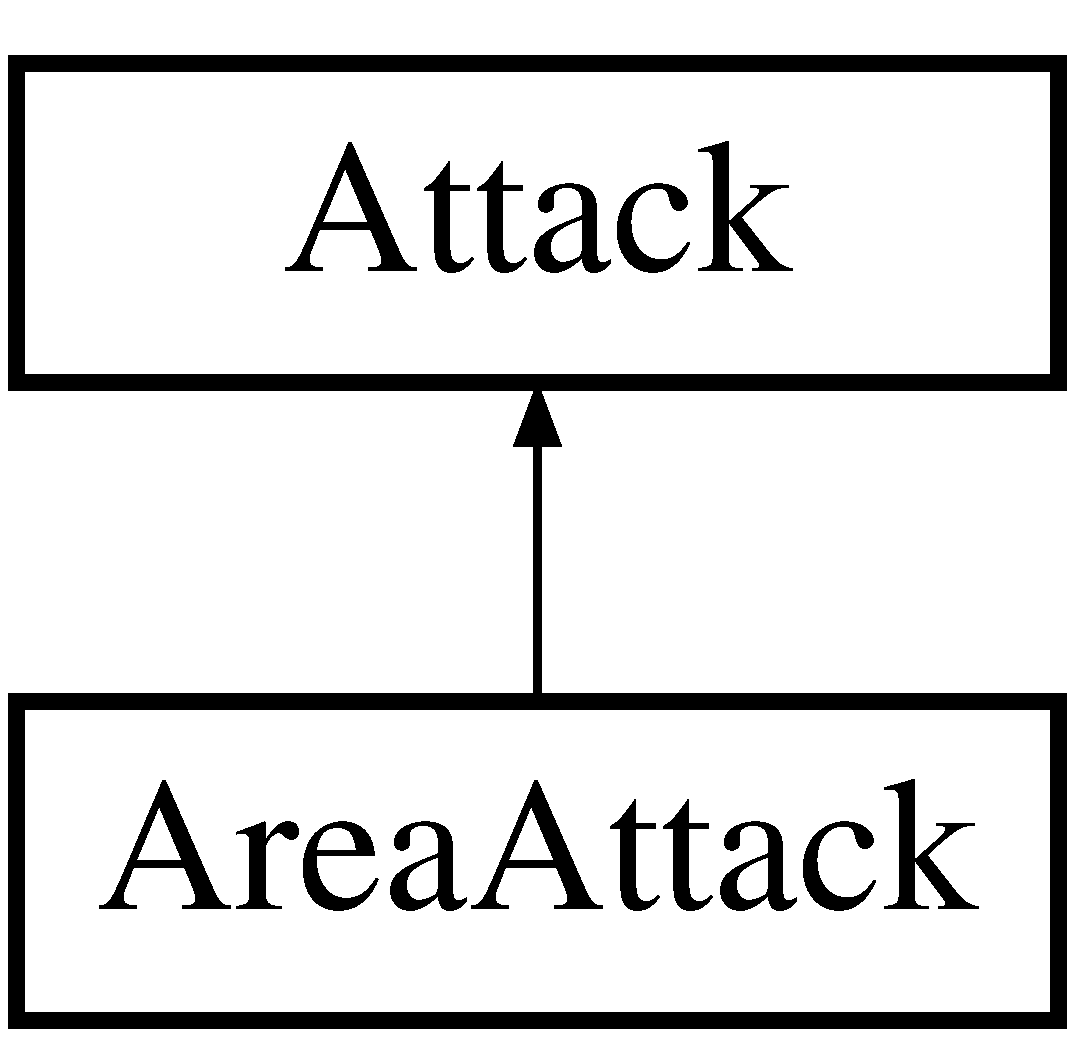
\includegraphics[height=2.000000cm]{class_area_attack}
\end{center}
\end{figure}
\subsection*{Public Member Functions}
\begin{DoxyCompactItemize}
\item 
\hyperlink{class_area_attack_a02cc5e5bf2f6883f144f6ad5eba57db1}{Area\+Attack} ()
\item 
virtual \hyperlink{class_area_attack_aa1e868a7e1be4faff11efd88bab9aed8}{$\sim$\+Area\+Attack} ()
\item 
vector$<$ shared\+\_\+ptr$<$ \hyperlink{class_enemy}{Enemy} $>$ $>$ \hyperlink{class_area_attack_a028bc8efccb4cf22b9ceab22302f0c5a}{get\+Target} ()
\item 
void \hyperlink{class_area_attack_a1609522af5e5d2b93e2a48ece5f75f75}{attack\+Animation} (sf\+::\+Render\+Window \&w) override
\item 
void \hyperlink{class_area_attack_a959d58d03e60e0df7d33ceb14866a496}{resolve} (sf\+::\+Render\+Window \&w) override
\item 
bool \hyperlink{class_area_attack_a65a1e2c1cdfb5873354b6fed903c0e6a}{has\+Enemy\+In\+Range} ()
\end{DoxyCompactItemize}
\subsection*{Additional Inherited Members}


\subsection{Constructor \& Destructor Documentation}
\hypertarget{class_area_attack_a02cc5e5bf2f6883f144f6ad5eba57db1}{\index{Area\+Attack@{Area\+Attack}!Area\+Attack@{Area\+Attack}}
\index{Area\+Attack@{Area\+Attack}!Area\+Attack@{Area\+Attack}}
\subsubsection[{Area\+Attack}]{\setlength{\rightskip}{0pt plus 5cm}Area\+Attack\+::\+Area\+Attack (
\begin{DoxyParamCaption}
{}
\end{DoxyParamCaption}
)}}\label{class_area_attack_a02cc5e5bf2f6883f144f6ad5eba57db1}
\hypertarget{class_area_attack_aa1e868a7e1be4faff11efd88bab9aed8}{\index{Area\+Attack@{Area\+Attack}!````~Area\+Attack@{$\sim$\+Area\+Attack}}
\index{````~Area\+Attack@{$\sim$\+Area\+Attack}!Area\+Attack@{Area\+Attack}}
\subsubsection[{$\sim$\+Area\+Attack}]{\setlength{\rightskip}{0pt plus 5cm}Area\+Attack\+::$\sim$\+Area\+Attack (
\begin{DoxyParamCaption}
{}
\end{DoxyParamCaption}
)\hspace{0.3cm}{\ttfamily [virtual]}}}\label{class_area_attack_aa1e868a7e1be4faff11efd88bab9aed8}


\subsection{Member Function Documentation}
\hypertarget{class_area_attack_a1609522af5e5d2b93e2a48ece5f75f75}{\index{Area\+Attack@{Area\+Attack}!attack\+Animation@{attack\+Animation}}
\index{attack\+Animation@{attack\+Animation}!Area\+Attack@{Area\+Attack}}
\subsubsection[{attack\+Animation}]{\setlength{\rightskip}{0pt plus 5cm}void Area\+Attack\+::attack\+Animation (
\begin{DoxyParamCaption}
\item[{sf\+::\+Render\+Window \&}]{w}
\end{DoxyParamCaption}
)\hspace{0.3cm}{\ttfamily [override]}, {\ttfamily [virtual]}}}\label{class_area_attack_a1609522af5e5d2b93e2a48ece5f75f75}


Implements \hyperlink{class_attack_a893c5523d0c10531a99e0c84caf87ef6}{Attack}.

\hypertarget{class_area_attack_a028bc8efccb4cf22b9ceab22302f0c5a}{\index{Area\+Attack@{Area\+Attack}!get\+Target@{get\+Target}}
\index{get\+Target@{get\+Target}!Area\+Attack@{Area\+Attack}}
\subsubsection[{get\+Target}]{\setlength{\rightskip}{0pt plus 5cm}vector$<$ shared\+\_\+ptr$<$ {\bf Enemy} $>$ $>$ Area\+Attack\+::get\+Target (
\begin{DoxyParamCaption}
{}
\end{DoxyParamCaption}
)}}\label{class_area_attack_a028bc8efccb4cf22b9ceab22302f0c5a}
\hypertarget{class_area_attack_a65a1e2c1cdfb5873354b6fed903c0e6a}{\index{Area\+Attack@{Area\+Attack}!has\+Enemy\+In\+Range@{has\+Enemy\+In\+Range}}
\index{has\+Enemy\+In\+Range@{has\+Enemy\+In\+Range}!Area\+Attack@{Area\+Attack}}
\subsubsection[{has\+Enemy\+In\+Range}]{\setlength{\rightskip}{0pt plus 5cm}bool Area\+Attack\+::has\+Enemy\+In\+Range (
\begin{DoxyParamCaption}
{}
\end{DoxyParamCaption}
)}}\label{class_area_attack_a65a1e2c1cdfb5873354b6fed903c0e6a}
\hypertarget{class_area_attack_a959d58d03e60e0df7d33ceb14866a496}{\index{Area\+Attack@{Area\+Attack}!resolve@{resolve}}
\index{resolve@{resolve}!Area\+Attack@{Area\+Attack}}
\subsubsection[{resolve}]{\setlength{\rightskip}{0pt plus 5cm}void Area\+Attack\+::resolve (
\begin{DoxyParamCaption}
\item[{sf\+::\+Render\+Window \&}]{w}
\end{DoxyParamCaption}
)\hspace{0.3cm}{\ttfamily [override]}, {\ttfamily [virtual]}}}\label{class_area_attack_a959d58d03e60e0df7d33ceb14866a496}


Implements \hyperlink{class_attack_aa3cd911d37e61278a9eeeb6d60303102}{Attack}.



The documentation for this class was generated from the following files\+:\begin{DoxyCompactItemize}
\item 
D\+:/\+Tower\+Defense/\+Tower\+Defense/\hyperlink{_area_attack_8h}{Area\+Attack.\+h}\item 
D\+:/\+Tower\+Defense/\+Tower\+Defense/\hyperlink{_area_attack_8cpp}{Area\+Attack.\+cpp}\end{DoxyCompactItemize}

\hypertarget{class_attack}{\section{Attack Class Reference}
\label{class_attack}\index{Attack@{Attack}}
}


{\ttfamily \#include $<$Attack.\+h$>$}

Inheritance diagram for Attack\+:\begin{figure}[H]
\begin{center}
\leavevmode
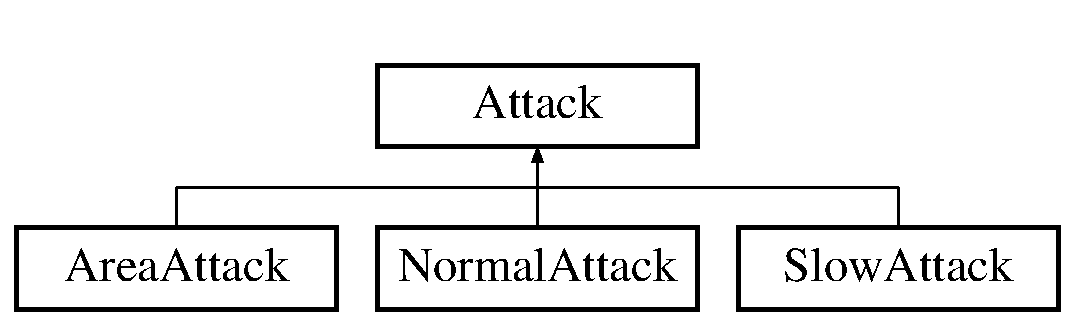
\includegraphics[height=2.000000cm]{class_attack}
\end{center}
\end{figure}
\subsection*{Public Member Functions}
\begin{DoxyCompactItemize}
\item 
\hyperlink{class_attack_aa2f391755dbfa049a6bc2991fae80017}{Attack} ()
\item 
\hyperlink{class_attack_a6d3c8266507e4ac0102ab40847f478fe}{$\sim$\+Attack} ()
\item 
float \hyperlink{class_attack_a03f55a2222756b756522c90de785a254}{get\+Damage} ()
\item 
float \hyperlink{class_attack_ae6eb96b3cd44a8c90e88d09de05224f3}{get\+Slow\+Amount} ()
\item 
void \hyperlink{class_attack_a1cd547335be67bf657f65d43ebc5f944}{set\+Damage} (float m\+Damage)
\item 
void \hyperlink{class_attack_a75d9cd8b8e20236cbd2c81dd7ede76a1}{set\+Slow\+Amount} (float m\+Slow\+Amount)
\item 
void \hyperlink{class_attack_a4fc62d7217e5e23232ee97f67a22becd}{set\+Center} (sf\+::\+Vector2i m\+Center)
\item 
void \hyperlink{class_attack_af5eaeef073b1cabb2baaa7a32489afa4}{set\+Range} (float m\+Range)
\item 
void \hyperlink{class_attack_a6800223da82f1ccf295b9d0a1940cb9e}{set\+Speed} (int m\+Speed)
\item 
void \hyperlink{class_attack_a096521777c0ac31ee453d42ab2bdc8aa}{set\+Timer} (int m\+Timer)
\item 
shared\+\_\+ptr$<$ \hyperlink{class_enemy}{Enemy} $>$ \hyperlink{class_attack_a2181ac078d36264732cd16cb3b80efee}{get\+Target} ()
\item 
sf\+::\+Vector2i \hyperlink{class_attack_a03bd157da34103a2a3a79fcd53e65e12}{get\+Center} ()
\item 
void \hyperlink{class_attack_ab6ca4fe8a0516671230a225af069e3d2}{set\+Attack\+Ray\+Angle} (shared\+\_\+ptr$<$ \hyperlink{class_enemy}{Enemy} $>$ target)
\item 
virtual void \hyperlink{class_attack_a893c5523d0c10531a99e0c84caf87ef6}{attack\+Animation} (sf\+::\+Render\+Window \&w)=0
\item 
virtual void \hyperlink{class_attack_aa3cd911d37e61278a9eeeb6d60303102}{resolve} (sf\+::\+Render\+Window \&w)=0
\end{DoxyCompactItemize}
\subsection*{Protected Attributes}
\begin{DoxyCompactItemize}
\item 
float \hyperlink{class_attack_ada6394cfb35919b6f84cfb390eb7c9ab}{slow\+Amount}
\item 
float \hyperlink{class_attack_aebc541003702819369c4645d425b8ba0}{damage}
\item 
float \hyperlink{class_attack_aa3207fc391fcc38836dc35e2b7d07cd8}{range}
\item 
sf\+::\+Vector2i \hyperlink{class_attack_a93137b1d93ca34ea21026225eeda24af}{center}
\item 
int \hyperlink{class_attack_aaeda94d2181b4f19f9d6e3f192289d67}{timer}
\item 
int \hyperlink{class_attack_adffcc8570d6503befe2646836893d466}{speed}
\item 
float \hyperlink{class_attack_ab318c12d748769f542a45839958a0b3f}{target\+Distance}
\item 
sf\+::\+Rectangle\+Shape \hyperlink{class_attack_a1b7bb04e9eca7ef43e5f916f766e01d4}{attack\+Ray}
\end{DoxyCompactItemize}


\subsection{Constructor \& Destructor Documentation}
\hypertarget{class_attack_aa2f391755dbfa049a6bc2991fae80017}{\index{Attack@{Attack}!Attack@{Attack}}
\index{Attack@{Attack}!Attack@{Attack}}
\subsubsection[{Attack}]{\setlength{\rightskip}{0pt plus 5cm}Attack\+::\+Attack (
\begin{DoxyParamCaption}
{}
\end{DoxyParamCaption}
)}}\label{class_attack_aa2f391755dbfa049a6bc2991fae80017}
\hypertarget{class_attack_a6d3c8266507e4ac0102ab40847f478fe}{\index{Attack@{Attack}!````~Attack@{$\sim$\+Attack}}
\index{````~Attack@{$\sim$\+Attack}!Attack@{Attack}}
\subsubsection[{$\sim$\+Attack}]{\setlength{\rightskip}{0pt plus 5cm}Attack\+::$\sim$\+Attack (
\begin{DoxyParamCaption}
{}
\end{DoxyParamCaption}
)}}\label{class_attack_a6d3c8266507e4ac0102ab40847f478fe}


\subsection{Member Function Documentation}
\hypertarget{class_attack_a893c5523d0c10531a99e0c84caf87ef6}{\index{Attack@{Attack}!attack\+Animation@{attack\+Animation}}
\index{attack\+Animation@{attack\+Animation}!Attack@{Attack}}
\subsubsection[{attack\+Animation}]{\setlength{\rightskip}{0pt plus 5cm}virtual void Attack\+::attack\+Animation (
\begin{DoxyParamCaption}
\item[{sf\+::\+Render\+Window \&}]{w}
\end{DoxyParamCaption}
)\hspace{0.3cm}{\ttfamily [pure virtual]}}}\label{class_attack_a893c5523d0c10531a99e0c84caf87ef6}


Implemented in \hyperlink{class_area_attack_a1609522af5e5d2b93e2a48ece5f75f75}{Area\+Attack}, \hyperlink{class_normal_attack_ae56877c3a110e0b4541776b89e252b10}{Normal\+Attack}, and \hyperlink{class_slow_attack_afa5a9af6a5b26bdb4168ee5a909433a6}{Slow\+Attack}.

\hypertarget{class_attack_a03bd157da34103a2a3a79fcd53e65e12}{\index{Attack@{Attack}!get\+Center@{get\+Center}}
\index{get\+Center@{get\+Center}!Attack@{Attack}}
\subsubsection[{get\+Center}]{\setlength{\rightskip}{0pt plus 5cm}sf\+::\+Vector2i Attack\+::get\+Center (
\begin{DoxyParamCaption}
{}
\end{DoxyParamCaption}
)}}\label{class_attack_a03bd157da34103a2a3a79fcd53e65e12}
\hypertarget{class_attack_a03f55a2222756b756522c90de785a254}{\index{Attack@{Attack}!get\+Damage@{get\+Damage}}
\index{get\+Damage@{get\+Damage}!Attack@{Attack}}
\subsubsection[{get\+Damage}]{\setlength{\rightskip}{0pt plus 5cm}float Attack\+::get\+Damage (
\begin{DoxyParamCaption}
{}
\end{DoxyParamCaption}
)}}\label{class_attack_a03f55a2222756b756522c90de785a254}
\hypertarget{class_attack_ae6eb96b3cd44a8c90e88d09de05224f3}{\index{Attack@{Attack}!get\+Slow\+Amount@{get\+Slow\+Amount}}
\index{get\+Slow\+Amount@{get\+Slow\+Amount}!Attack@{Attack}}
\subsubsection[{get\+Slow\+Amount}]{\setlength{\rightskip}{0pt plus 5cm}float Attack\+::get\+Slow\+Amount (
\begin{DoxyParamCaption}
{}
\end{DoxyParamCaption}
)}}\label{class_attack_ae6eb96b3cd44a8c90e88d09de05224f3}
\hypertarget{class_attack_a2181ac078d36264732cd16cb3b80efee}{\index{Attack@{Attack}!get\+Target@{get\+Target}}
\index{get\+Target@{get\+Target}!Attack@{Attack}}
\subsubsection[{get\+Target}]{\setlength{\rightskip}{0pt plus 5cm}shared\+\_\+ptr$<$ {\bf Enemy} $>$ Attack\+::get\+Target (
\begin{DoxyParamCaption}
{}
\end{DoxyParamCaption}
)}}\label{class_attack_a2181ac078d36264732cd16cb3b80efee}
\hypertarget{class_attack_aa3cd911d37e61278a9eeeb6d60303102}{\index{Attack@{Attack}!resolve@{resolve}}
\index{resolve@{resolve}!Attack@{Attack}}
\subsubsection[{resolve}]{\setlength{\rightskip}{0pt plus 5cm}virtual void Attack\+::resolve (
\begin{DoxyParamCaption}
\item[{sf\+::\+Render\+Window \&}]{w}
\end{DoxyParamCaption}
)\hspace{0.3cm}{\ttfamily [pure virtual]}}}\label{class_attack_aa3cd911d37e61278a9eeeb6d60303102}


Implemented in \hyperlink{class_area_attack_a959d58d03e60e0df7d33ceb14866a496}{Area\+Attack}, \hyperlink{class_normal_attack_a949ea101fc201897cd3cd262b2870388}{Normal\+Attack}, and \hyperlink{class_slow_attack_a73767803482c26adf9aae486faa7499c}{Slow\+Attack}.

\hypertarget{class_attack_ab6ca4fe8a0516671230a225af069e3d2}{\index{Attack@{Attack}!set\+Attack\+Ray\+Angle@{set\+Attack\+Ray\+Angle}}
\index{set\+Attack\+Ray\+Angle@{set\+Attack\+Ray\+Angle}!Attack@{Attack}}
\subsubsection[{set\+Attack\+Ray\+Angle}]{\setlength{\rightskip}{0pt plus 5cm}void Attack\+::set\+Attack\+Ray\+Angle (
\begin{DoxyParamCaption}
\item[{shared\+\_\+ptr$<$ {\bf Enemy} $>$}]{target}
\end{DoxyParamCaption}
)}}\label{class_attack_ab6ca4fe8a0516671230a225af069e3d2}
\hypertarget{class_attack_a4fc62d7217e5e23232ee97f67a22becd}{\index{Attack@{Attack}!set\+Center@{set\+Center}}
\index{set\+Center@{set\+Center}!Attack@{Attack}}
\subsubsection[{set\+Center}]{\setlength{\rightskip}{0pt plus 5cm}void Attack\+::set\+Center (
\begin{DoxyParamCaption}
\item[{sf\+::\+Vector2i}]{m\+Center}
\end{DoxyParamCaption}
)}}\label{class_attack_a4fc62d7217e5e23232ee97f67a22becd}
\hypertarget{class_attack_a1cd547335be67bf657f65d43ebc5f944}{\index{Attack@{Attack}!set\+Damage@{set\+Damage}}
\index{set\+Damage@{set\+Damage}!Attack@{Attack}}
\subsubsection[{set\+Damage}]{\setlength{\rightskip}{0pt plus 5cm}void Attack\+::set\+Damage (
\begin{DoxyParamCaption}
\item[{float}]{m\+Damage}
\end{DoxyParamCaption}
)}}\label{class_attack_a1cd547335be67bf657f65d43ebc5f944}
\hypertarget{class_attack_af5eaeef073b1cabb2baaa7a32489afa4}{\index{Attack@{Attack}!set\+Range@{set\+Range}}
\index{set\+Range@{set\+Range}!Attack@{Attack}}
\subsubsection[{set\+Range}]{\setlength{\rightskip}{0pt plus 5cm}void Attack\+::set\+Range (
\begin{DoxyParamCaption}
\item[{float}]{m\+Range}
\end{DoxyParamCaption}
)}}\label{class_attack_af5eaeef073b1cabb2baaa7a32489afa4}
\hypertarget{class_attack_a75d9cd8b8e20236cbd2c81dd7ede76a1}{\index{Attack@{Attack}!set\+Slow\+Amount@{set\+Slow\+Amount}}
\index{set\+Slow\+Amount@{set\+Slow\+Amount}!Attack@{Attack}}
\subsubsection[{set\+Slow\+Amount}]{\setlength{\rightskip}{0pt plus 5cm}void Attack\+::set\+Slow\+Amount (
\begin{DoxyParamCaption}
\item[{float}]{m\+Slow\+Amount}
\end{DoxyParamCaption}
)}}\label{class_attack_a75d9cd8b8e20236cbd2c81dd7ede76a1}
\hypertarget{class_attack_a6800223da82f1ccf295b9d0a1940cb9e}{\index{Attack@{Attack}!set\+Speed@{set\+Speed}}
\index{set\+Speed@{set\+Speed}!Attack@{Attack}}
\subsubsection[{set\+Speed}]{\setlength{\rightskip}{0pt plus 5cm}void Attack\+::set\+Speed (
\begin{DoxyParamCaption}
\item[{int}]{m\+Speed}
\end{DoxyParamCaption}
)}}\label{class_attack_a6800223da82f1ccf295b9d0a1940cb9e}
\hypertarget{class_attack_a096521777c0ac31ee453d42ab2bdc8aa}{\index{Attack@{Attack}!set\+Timer@{set\+Timer}}
\index{set\+Timer@{set\+Timer}!Attack@{Attack}}
\subsubsection[{set\+Timer}]{\setlength{\rightskip}{0pt plus 5cm}void Attack\+::set\+Timer (
\begin{DoxyParamCaption}
\item[{int}]{m\+Timer}
\end{DoxyParamCaption}
)}}\label{class_attack_a096521777c0ac31ee453d42ab2bdc8aa}


\subsection{Member Data Documentation}
\hypertarget{class_attack_a1b7bb04e9eca7ef43e5f916f766e01d4}{\index{Attack@{Attack}!attack\+Ray@{attack\+Ray}}
\index{attack\+Ray@{attack\+Ray}!Attack@{Attack}}
\subsubsection[{attack\+Ray}]{\setlength{\rightskip}{0pt plus 5cm}sf\+::\+Rectangle\+Shape Attack\+::attack\+Ray\hspace{0.3cm}{\ttfamily [protected]}}}\label{class_attack_a1b7bb04e9eca7ef43e5f916f766e01d4}
\hypertarget{class_attack_a93137b1d93ca34ea21026225eeda24af}{\index{Attack@{Attack}!center@{center}}
\index{center@{center}!Attack@{Attack}}
\subsubsection[{center}]{\setlength{\rightskip}{0pt plus 5cm}sf\+::\+Vector2i Attack\+::center\hspace{0.3cm}{\ttfamily [protected]}}}\label{class_attack_a93137b1d93ca34ea21026225eeda24af}
\hypertarget{class_attack_aebc541003702819369c4645d425b8ba0}{\index{Attack@{Attack}!damage@{damage}}
\index{damage@{damage}!Attack@{Attack}}
\subsubsection[{damage}]{\setlength{\rightskip}{0pt plus 5cm}float Attack\+::damage\hspace{0.3cm}{\ttfamily [protected]}}}\label{class_attack_aebc541003702819369c4645d425b8ba0}
\hypertarget{class_attack_aa3207fc391fcc38836dc35e2b7d07cd8}{\index{Attack@{Attack}!range@{range}}
\index{range@{range}!Attack@{Attack}}
\subsubsection[{range}]{\setlength{\rightskip}{0pt plus 5cm}float Attack\+::range\hspace{0.3cm}{\ttfamily [protected]}}}\label{class_attack_aa3207fc391fcc38836dc35e2b7d07cd8}
\hypertarget{class_attack_ada6394cfb35919b6f84cfb390eb7c9ab}{\index{Attack@{Attack}!slow\+Amount@{slow\+Amount}}
\index{slow\+Amount@{slow\+Amount}!Attack@{Attack}}
\subsubsection[{slow\+Amount}]{\setlength{\rightskip}{0pt plus 5cm}float Attack\+::slow\+Amount\hspace{0.3cm}{\ttfamily [protected]}}}\label{class_attack_ada6394cfb35919b6f84cfb390eb7c9ab}
\hypertarget{class_attack_adffcc8570d6503befe2646836893d466}{\index{Attack@{Attack}!speed@{speed}}
\index{speed@{speed}!Attack@{Attack}}
\subsubsection[{speed}]{\setlength{\rightskip}{0pt plus 5cm}int Attack\+::speed\hspace{0.3cm}{\ttfamily [protected]}}}\label{class_attack_adffcc8570d6503befe2646836893d466}
\hypertarget{class_attack_ab318c12d748769f542a45839958a0b3f}{\index{Attack@{Attack}!target\+Distance@{target\+Distance}}
\index{target\+Distance@{target\+Distance}!Attack@{Attack}}
\subsubsection[{target\+Distance}]{\setlength{\rightskip}{0pt plus 5cm}float Attack\+::target\+Distance\hspace{0.3cm}{\ttfamily [protected]}}}\label{class_attack_ab318c12d748769f542a45839958a0b3f}
\hypertarget{class_attack_aaeda94d2181b4f19f9d6e3f192289d67}{\index{Attack@{Attack}!timer@{timer}}
\index{timer@{timer}!Attack@{Attack}}
\subsubsection[{timer}]{\setlength{\rightskip}{0pt plus 5cm}int Attack\+::timer\hspace{0.3cm}{\ttfamily [protected]}}}\label{class_attack_aaeda94d2181b4f19f9d6e3f192289d67}


The documentation for this class was generated from the following files\+:\begin{DoxyCompactItemize}
\item 
D\+:/\+Tower\+Defense/\+Tower\+Defense/\hyperlink{_attack_8h}{Attack.\+h}\item 
D\+:/\+Tower\+Defense/\+Tower\+Defense/\hyperlink{_attack_8cpp}{Attack.\+cpp}\end{DoxyCompactItemize}

\hypertarget{class_audio_manager}{\section{Audio\+Manager Class Reference}
\label{class_audio_manager}\index{Audio\+Manager@{Audio\+Manager}}
}


{\ttfamily \#include $<$Audio\+Manager.\+h$>$}

\subsection*{Public Member Functions}
\begin{DoxyCompactItemize}
\item 
\hyperlink{class_audio_manager_ab9185d5d1fac7694ef1b86615c06b30e}{Audio\+Manager} (bool)
\item 
\hyperlink{class_audio_manager_ae59d8605c1d706e7bab47d4e8f900d09}{Audio\+Manager} ()
\item 
void \hyperlink{class_audio_manager_a413714ef87ed432842fb9c3571a1d3f2}{mute} ()
\item 
bool \hyperlink{class_audio_manager_abc84cf825cff23791751a2aadce32b43}{play} ()
\item 
bool \hyperlink{class_audio_manager_a24d2077e232ef579229e7c70205e37a4}{is\+Mute} ()
\end{DoxyCompactItemize}
\subsection*{Static Public Member Functions}
\begin{DoxyCompactItemize}
\item 
static shared\+\_\+ptr$<$ \hyperlink{class_audio_manager}{Audio\+Manager} $>$ \hyperlink{class_audio_manager_a9bd57da07855563c46daaa9d1aec5d29}{get\+Audio\+Manager} ()
\end{DoxyCompactItemize}


\subsection{Constructor \& Destructor Documentation}
\hypertarget{class_audio_manager_ab9185d5d1fac7694ef1b86615c06b30e}{\index{Audio\+Manager@{Audio\+Manager}!Audio\+Manager@{Audio\+Manager}}
\index{Audio\+Manager@{Audio\+Manager}!Audio\+Manager@{Audio\+Manager}}
\subsubsection[{Audio\+Manager}]{\setlength{\rightskip}{0pt plus 5cm}Audio\+Manager\+::\+Audio\+Manager (
\begin{DoxyParamCaption}
\item[{bool}]{b}
\end{DoxyParamCaption}
)}}\label{class_audio_manager_ab9185d5d1fac7694ef1b86615c06b30e}
\hypertarget{class_audio_manager_ae59d8605c1d706e7bab47d4e8f900d09}{\index{Audio\+Manager@{Audio\+Manager}!Audio\+Manager@{Audio\+Manager}}
\index{Audio\+Manager@{Audio\+Manager}!Audio\+Manager@{Audio\+Manager}}
\subsubsection[{Audio\+Manager}]{\setlength{\rightskip}{0pt plus 5cm}Audio\+Manager\+::\+Audio\+Manager (
\begin{DoxyParamCaption}
{}
\end{DoxyParamCaption}
)}}\label{class_audio_manager_ae59d8605c1d706e7bab47d4e8f900d09}


\subsection{Member Function Documentation}
\hypertarget{class_audio_manager_a9bd57da07855563c46daaa9d1aec5d29}{\index{Audio\+Manager@{Audio\+Manager}!get\+Audio\+Manager@{get\+Audio\+Manager}}
\index{get\+Audio\+Manager@{get\+Audio\+Manager}!Audio\+Manager@{Audio\+Manager}}
\subsubsection[{get\+Audio\+Manager}]{\setlength{\rightskip}{0pt plus 5cm}shared\+\_\+ptr$<$ {\bf Audio\+Manager} $>$ Audio\+Manager\+::get\+Audio\+Manager (
\begin{DoxyParamCaption}
{}
\end{DoxyParamCaption}
)\hspace{0.3cm}{\ttfamily [static]}}}\label{class_audio_manager_a9bd57da07855563c46daaa9d1aec5d29}
\hypertarget{class_audio_manager_a24d2077e232ef579229e7c70205e37a4}{\index{Audio\+Manager@{Audio\+Manager}!is\+Mute@{is\+Mute}}
\index{is\+Mute@{is\+Mute}!Audio\+Manager@{Audio\+Manager}}
\subsubsection[{is\+Mute}]{\setlength{\rightskip}{0pt plus 5cm}bool Audio\+Manager\+::is\+Mute (
\begin{DoxyParamCaption}
{}
\end{DoxyParamCaption}
)}}\label{class_audio_manager_a24d2077e232ef579229e7c70205e37a4}
\hypertarget{class_audio_manager_a413714ef87ed432842fb9c3571a1d3f2}{\index{Audio\+Manager@{Audio\+Manager}!mute@{mute}}
\index{mute@{mute}!Audio\+Manager@{Audio\+Manager}}
\subsubsection[{mute}]{\setlength{\rightskip}{0pt plus 5cm}void Audio\+Manager\+::mute (
\begin{DoxyParamCaption}
{}
\end{DoxyParamCaption}
)}}\label{class_audio_manager_a413714ef87ed432842fb9c3571a1d3f2}
\hypertarget{class_audio_manager_abc84cf825cff23791751a2aadce32b43}{\index{Audio\+Manager@{Audio\+Manager}!play@{play}}
\index{play@{play}!Audio\+Manager@{Audio\+Manager}}
\subsubsection[{play}]{\setlength{\rightskip}{0pt plus 5cm}bool Audio\+Manager\+::play (
\begin{DoxyParamCaption}
{}
\end{DoxyParamCaption}
)}}\label{class_audio_manager_abc84cf825cff23791751a2aadce32b43}


The documentation for this class was generated from the following files\+:\begin{DoxyCompactItemize}
\item 
D\+:/\+Tower\+Defense/\+Tower\+Defense/\hyperlink{_audio_manager_8h}{Audio\+Manager.\+h}\item 
D\+:/\+Tower\+Defense/\+Tower\+Defense/\hyperlink{_audio_manager_8cpp}{Audio\+Manager.\+cpp}\end{DoxyCompactItemize}

\hypertarget{class_bomb_enemy}{\section{Bomb\+Enemy Class Reference}
\label{class_bomb_enemy}\index{Bomb\+Enemy@{Bomb\+Enemy}}
}


{\ttfamily \#include $<$Bomb\+Enemy.\+h$>$}

Inheritance diagram for Bomb\+Enemy\+:\begin{figure}[H]
\begin{center}
\leavevmode
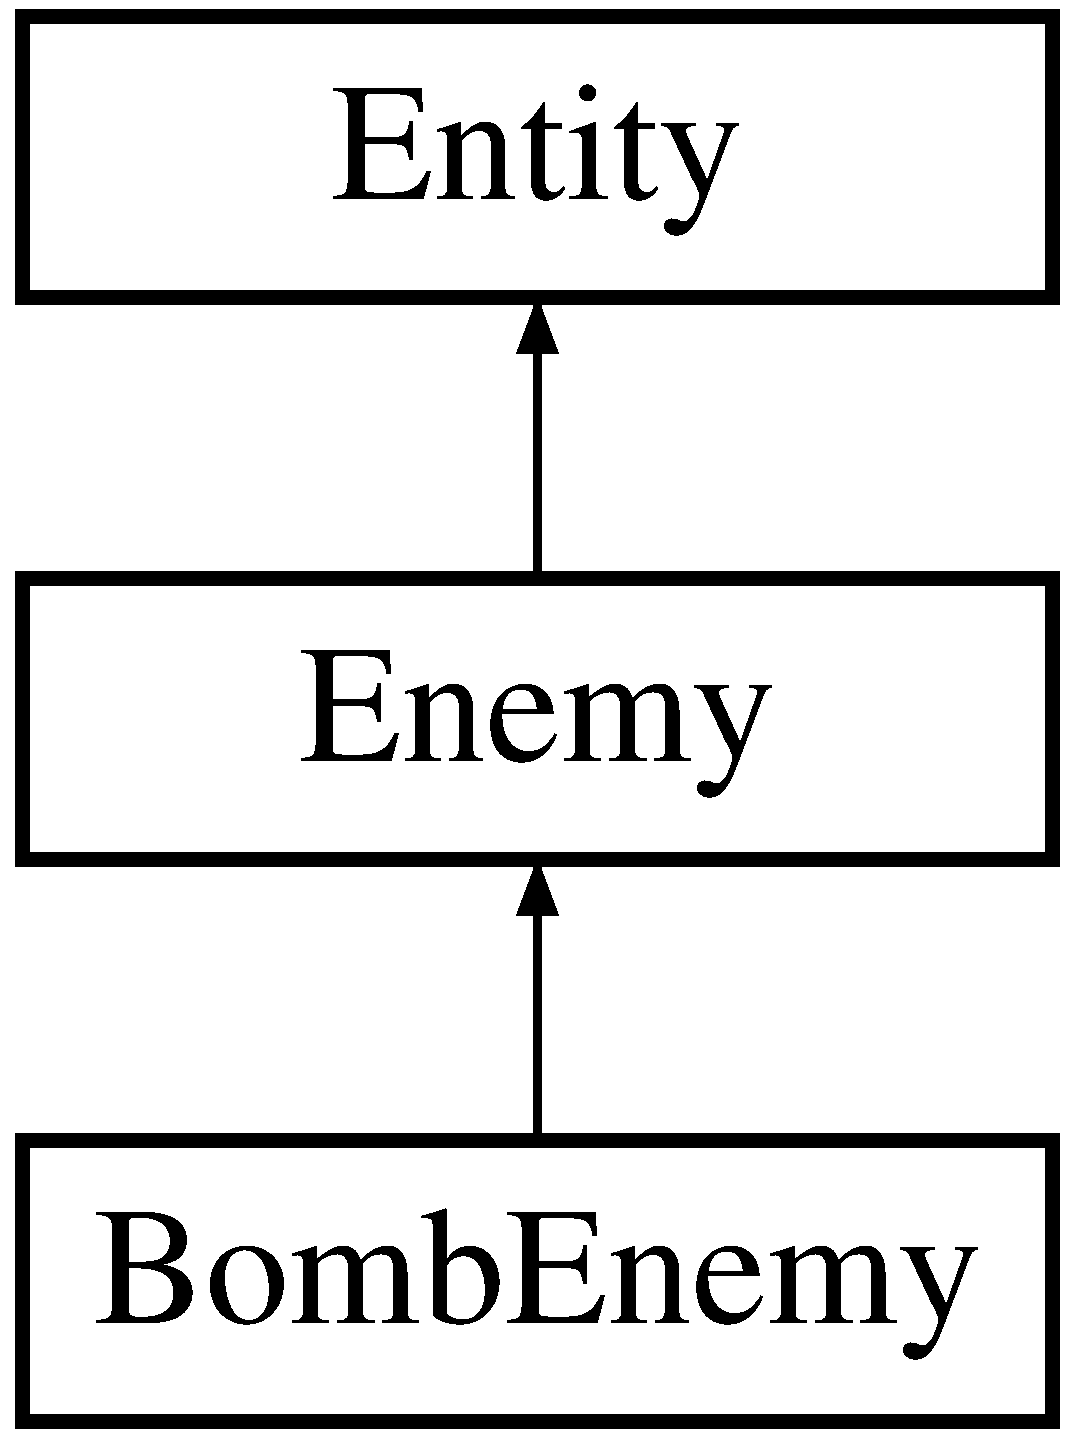
\includegraphics[height=3.000000cm]{class_bomb_enemy}
\end{center}
\end{figure}
\subsection*{Public Member Functions}
\begin{DoxyCompactItemize}
\item 
\hyperlink{class_bomb_enemy_a6b23badbfab051daf75ef8c10bfcd915}{Bomb\+Enemy} ()
\item 
\hyperlink{class_bomb_enemy_a3d5bbfa65313a43603d1a23cd66f9cd1}{Bomb\+Enemy} (int \hyperlink{class_enemy_a278d70100af07c946743db1b7a1a9f59}{hp}, float \hyperlink{class_enemy_a9bb5d74024760e604c41ba79cc7da892}{defence}, int \hyperlink{class_enemy_a1d9a86d110b87f3cc55b40d1bdb59eb5}{bounty}, int \hyperlink{class_enemy_abc49d5a2cef917c8ece8a16547f8efee}{score\+Value}, int trigger, sf\+::\+Sprite \hyperlink{class_entity_a48ef4ab143b8d0211877c9f6be42e824}{sprite}, float \hyperlink{class_entity_a1de3d8d9ab8088f61e6726069b26fa60}{speed})
\item 
virtual \hyperlink{class_bomb_enemy_a8a79819bd365d564c77058f0fd9495c4}{$\sim$\+Bomb\+Enemy} ()
\item 
string \hyperlink{class_bomb_enemy_a6fde389b791b1d977caa01a15a66df1c}{test} ()
\item 
int \hyperlink{class_bomb_enemy_a9d1db939bea4bf8a9fc4b5bfead03fc3}{get\+Trigger} ()
\item 
int \hyperlink{class_bomb_enemy_a5a8244c65fbf9f8fceb07080e11ddbe8}{get\+Timer} ()
\item 
void \hyperlink{class_bomb_enemy_a0a984610f97fe852884e0d00d0461a9c}{explode} ()
\item 
void \hyperlink{class_bomb_enemy_a7eb5ed711a40cbd0af016450bf59b0e4}{Trigger\+Count\+Down} ()
\item 
void \hyperlink{class_bomb_enemy_a15e34ebba40eaf805ffe179ec4c9a2af}{check\+Count\+Down} ()
\item 
bool \hyperlink{class_bomb_enemy_ae421414fdc87d4cb92bdc6975a3b28b4}{move} () override
\end{DoxyCompactItemize}
\subsection*{Additional Inherited Members}


\subsection{Constructor \& Destructor Documentation}
\hypertarget{class_bomb_enemy_a6b23badbfab051daf75ef8c10bfcd915}{\index{Bomb\+Enemy@{Bomb\+Enemy}!Bomb\+Enemy@{Bomb\+Enemy}}
\index{Bomb\+Enemy@{Bomb\+Enemy}!Bomb\+Enemy@{Bomb\+Enemy}}
\subsubsection[{Bomb\+Enemy}]{\setlength{\rightskip}{0pt plus 5cm}Bomb\+Enemy\+::\+Bomb\+Enemy (
\begin{DoxyParamCaption}
{}
\end{DoxyParamCaption}
)}}\label{class_bomb_enemy_a6b23badbfab051daf75ef8c10bfcd915}
\hypertarget{class_bomb_enemy_a3d5bbfa65313a43603d1a23cd66f9cd1}{\index{Bomb\+Enemy@{Bomb\+Enemy}!Bomb\+Enemy@{Bomb\+Enemy}}
\index{Bomb\+Enemy@{Bomb\+Enemy}!Bomb\+Enemy@{Bomb\+Enemy}}
\subsubsection[{Bomb\+Enemy}]{\setlength{\rightskip}{0pt plus 5cm}Bomb\+Enemy\+::\+Bomb\+Enemy (
\begin{DoxyParamCaption}
\item[{int}]{hp, }
\item[{float}]{defence, }
\item[{int}]{bounty, }
\item[{int}]{score\+Value, }
\item[{int}]{trigger, }
\item[{sf\+::\+Sprite}]{sprite, }
\item[{float}]{speed}
\end{DoxyParamCaption}
)}}\label{class_bomb_enemy_a3d5bbfa65313a43603d1a23cd66f9cd1}
\hypertarget{class_bomb_enemy_a8a79819bd365d564c77058f0fd9495c4}{\index{Bomb\+Enemy@{Bomb\+Enemy}!````~Bomb\+Enemy@{$\sim$\+Bomb\+Enemy}}
\index{````~Bomb\+Enemy@{$\sim$\+Bomb\+Enemy}!Bomb\+Enemy@{Bomb\+Enemy}}
\subsubsection[{$\sim$\+Bomb\+Enemy}]{\setlength{\rightskip}{0pt plus 5cm}virtual Bomb\+Enemy\+::$\sim$\+Bomb\+Enemy (
\begin{DoxyParamCaption}
{}
\end{DoxyParamCaption}
)\hspace{0.3cm}{\ttfamily [inline]}, {\ttfamily [virtual]}}}\label{class_bomb_enemy_a8a79819bd365d564c77058f0fd9495c4}


\subsection{Member Function Documentation}
\hypertarget{class_bomb_enemy_a15e34ebba40eaf805ffe179ec4c9a2af}{\index{Bomb\+Enemy@{Bomb\+Enemy}!check\+Count\+Down@{check\+Count\+Down}}
\index{check\+Count\+Down@{check\+Count\+Down}!Bomb\+Enemy@{Bomb\+Enemy}}
\subsubsection[{check\+Count\+Down}]{\setlength{\rightskip}{0pt plus 5cm}void Bomb\+Enemy\+::check\+Count\+Down (
\begin{DoxyParamCaption}
{}
\end{DoxyParamCaption}
)}}\label{class_bomb_enemy_a15e34ebba40eaf805ffe179ec4c9a2af}
\hypertarget{class_bomb_enemy_a0a984610f97fe852884e0d00d0461a9c}{\index{Bomb\+Enemy@{Bomb\+Enemy}!explode@{explode}}
\index{explode@{explode}!Bomb\+Enemy@{Bomb\+Enemy}}
\subsubsection[{explode}]{\setlength{\rightskip}{0pt plus 5cm}void Bomb\+Enemy\+::explode (
\begin{DoxyParamCaption}
{}
\end{DoxyParamCaption}
)}}\label{class_bomb_enemy_a0a984610f97fe852884e0d00d0461a9c}
\hypertarget{class_bomb_enemy_a5a8244c65fbf9f8fceb07080e11ddbe8}{\index{Bomb\+Enemy@{Bomb\+Enemy}!get\+Timer@{get\+Timer}}
\index{get\+Timer@{get\+Timer}!Bomb\+Enemy@{Bomb\+Enemy}}
\subsubsection[{get\+Timer}]{\setlength{\rightskip}{0pt plus 5cm}int Bomb\+Enemy\+::get\+Timer (
\begin{DoxyParamCaption}
{}
\end{DoxyParamCaption}
)}}\label{class_bomb_enemy_a5a8244c65fbf9f8fceb07080e11ddbe8}
\hypertarget{class_bomb_enemy_a9d1db939bea4bf8a9fc4b5bfead03fc3}{\index{Bomb\+Enemy@{Bomb\+Enemy}!get\+Trigger@{get\+Trigger}}
\index{get\+Trigger@{get\+Trigger}!Bomb\+Enemy@{Bomb\+Enemy}}
\subsubsection[{get\+Trigger}]{\setlength{\rightskip}{0pt plus 5cm}int Bomb\+Enemy\+::get\+Trigger (
\begin{DoxyParamCaption}
{}
\end{DoxyParamCaption}
)}}\label{class_bomb_enemy_a9d1db939bea4bf8a9fc4b5bfead03fc3}
\hypertarget{class_bomb_enemy_ae421414fdc87d4cb92bdc6975a3b28b4}{\index{Bomb\+Enemy@{Bomb\+Enemy}!move@{move}}
\index{move@{move}!Bomb\+Enemy@{Bomb\+Enemy}}
\subsubsection[{move}]{\setlength{\rightskip}{0pt plus 5cm}bool Bomb\+Enemy\+::move (
\begin{DoxyParamCaption}
{}
\end{DoxyParamCaption}
)\hspace{0.3cm}{\ttfamily [override]}, {\ttfamily [virtual]}}}\label{class_bomb_enemy_ae421414fdc87d4cb92bdc6975a3b28b4}


Reimplemented from \hyperlink{class_enemy_a8e0cfa58b8d27e254a0b3c6965962280}{Enemy}.

\hypertarget{class_bomb_enemy_a6fde389b791b1d977caa01a15a66df1c}{\index{Bomb\+Enemy@{Bomb\+Enemy}!test@{test}}
\index{test@{test}!Bomb\+Enemy@{Bomb\+Enemy}}
\subsubsection[{test}]{\setlength{\rightskip}{0pt plus 5cm}string Bomb\+Enemy\+::test (
\begin{DoxyParamCaption}
{}
\end{DoxyParamCaption}
)\hspace{0.3cm}{\ttfamily [inline]}, {\ttfamily [virtual]}}}\label{class_bomb_enemy_a6fde389b791b1d977caa01a15a66df1c}


Implements \hyperlink{class_enemy_a37b2bae4f5a9e8d673aeb28880ded0bc}{Enemy}.

\hypertarget{class_bomb_enemy_a7eb5ed711a40cbd0af016450bf59b0e4}{\index{Bomb\+Enemy@{Bomb\+Enemy}!Trigger\+Count\+Down@{Trigger\+Count\+Down}}
\index{Trigger\+Count\+Down@{Trigger\+Count\+Down}!Bomb\+Enemy@{Bomb\+Enemy}}
\subsubsection[{Trigger\+Count\+Down}]{\setlength{\rightskip}{0pt plus 5cm}void Bomb\+Enemy\+::\+Trigger\+Count\+Down (
\begin{DoxyParamCaption}
{}
\end{DoxyParamCaption}
)}}\label{class_bomb_enemy_a7eb5ed711a40cbd0af016450bf59b0e4}


The documentation for this class was generated from the following files\+:\begin{DoxyCompactItemize}
\item 
D\+:/\+Tower\+Defense/\+Tower\+Defense/\hyperlink{_bomb_enemy_8h}{Bomb\+Enemy.\+h}\item 
D\+:/\+Tower\+Defense/\+Tower\+Defense/\hyperlink{_bomb_enemy_8cpp}{Bomb\+Enemy.\+cpp}\end{DoxyCompactItemize}

\hypertarget{class_build_menu}{\section{Build\+Menu Class Reference}
\label{class_build_menu}\index{Build\+Menu@{Build\+Menu}}
}


{\ttfamily \#include $<$Build\+Menu.\+h$>$}

Inheritance diagram for Build\+Menu\+:\begin{figure}[H]
\begin{center}
\leavevmode
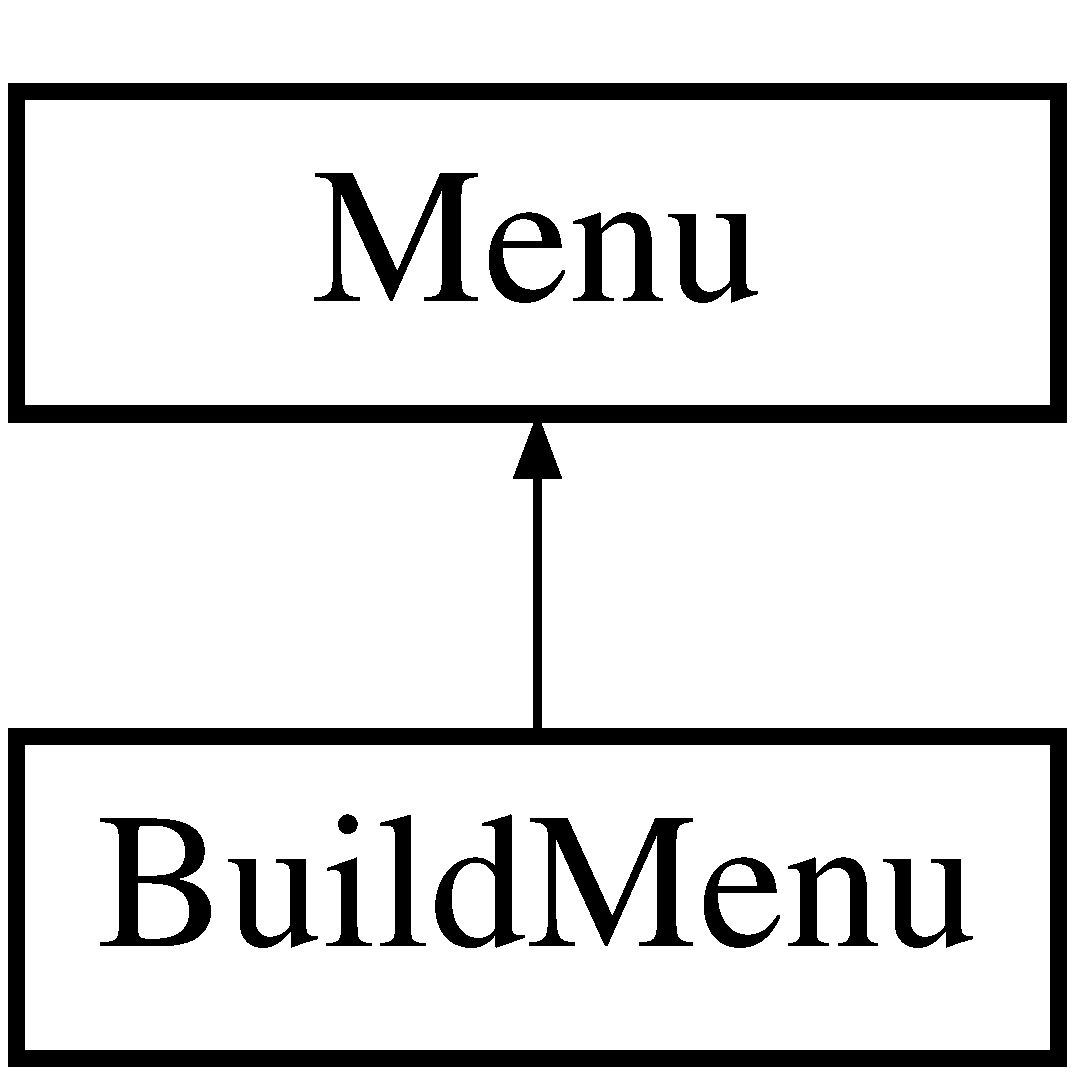
\includegraphics[height=2.000000cm]{class_build_menu}
\end{center}
\end{figure}
\subsection*{Public Member Functions}
\begin{DoxyCompactItemize}
\item 
\hyperlink{class_build_menu_acdbc901d204a90638bf17e71e4215311}{Build\+Menu} ()
\item 
\hyperlink{class_build_menu_ad63b1ba9611f30feb9446668566b0aa4}{Build\+Menu} (shared\+\_\+ptr$<$ \hyperlink{class_tile}{Tile} $>$)
\item 
\hyperlink{class_build_menu_a3683fde835c95da534d3bcbad731f6c8}{$\sim$\+Build\+Menu} ()
\item 
shared\+\_\+ptr$<$ \hyperlink{class_tile}{Tile} $>$ \hyperlink{class_build_menu_a5f4c9ee77c787c60468fe8c224637dfc}{get\+Tile} ()
\item 
void \hyperlink{class_build_menu_a769c90e895773e03cf3f12214ffde3e5}{buy\+Basic\+Tw} ()
\item 
void \hyperlink{class_build_menu_aba60e635a3ba452995e194bf3bd63304}{buy\+Slow\+Tw} ()
\item 
void \hyperlink{class_build_menu_a0608c73be6f0130d0bd827189572a702}{buy\+Money\+Tw} ()
\item 
void \hyperlink{class_build_menu_a0ad03076763bc89e1c2f855e448b9f61}{buy\+Sun\+Tw} ()
\item 
void \hyperlink{class_build_menu_a2d044954ea1713a15048630e104c7d2a}{resolve\+Event} (sf\+::\+Event)
\item 
void \hyperlink{class_build_menu_acbedc91d2b9c5ecf3d429612b95543a5}{draw} (sf\+::\+Render\+Window \&)
\item 
void \hyperlink{class_build_menu_a58efd17837e0cd60a9bd1852cf6eaadd}{close} ()
\end{DoxyCompactItemize}
\subsection*{Additional Inherited Members}


\subsection{Constructor \& Destructor Documentation}
\hypertarget{class_build_menu_acdbc901d204a90638bf17e71e4215311}{\index{Build\+Menu@{Build\+Menu}!Build\+Menu@{Build\+Menu}}
\index{Build\+Menu@{Build\+Menu}!Build\+Menu@{Build\+Menu}}
\subsubsection[{Build\+Menu}]{\setlength{\rightskip}{0pt plus 5cm}Build\+Menu\+::\+Build\+Menu (
\begin{DoxyParamCaption}
{}
\end{DoxyParamCaption}
)}}\label{class_build_menu_acdbc901d204a90638bf17e71e4215311}
\hypertarget{class_build_menu_ad63b1ba9611f30feb9446668566b0aa4}{\index{Build\+Menu@{Build\+Menu}!Build\+Menu@{Build\+Menu}}
\index{Build\+Menu@{Build\+Menu}!Build\+Menu@{Build\+Menu}}
\subsubsection[{Build\+Menu}]{\setlength{\rightskip}{0pt plus 5cm}Build\+Menu\+::\+Build\+Menu (
\begin{DoxyParamCaption}
\item[{shared\+\_\+ptr$<$ {\bf Tile} $>$}]{p\+Tile}
\end{DoxyParamCaption}
)}}\label{class_build_menu_ad63b1ba9611f30feb9446668566b0aa4}
\hypertarget{class_build_menu_a3683fde835c95da534d3bcbad731f6c8}{\index{Build\+Menu@{Build\+Menu}!````~Build\+Menu@{$\sim$\+Build\+Menu}}
\index{````~Build\+Menu@{$\sim$\+Build\+Menu}!Build\+Menu@{Build\+Menu}}
\subsubsection[{$\sim$\+Build\+Menu}]{\setlength{\rightskip}{0pt plus 5cm}Build\+Menu\+::$\sim$\+Build\+Menu (
\begin{DoxyParamCaption}
{}
\end{DoxyParamCaption}
)}}\label{class_build_menu_a3683fde835c95da534d3bcbad731f6c8}


\subsection{Member Function Documentation}
\hypertarget{class_build_menu_a769c90e895773e03cf3f12214ffde3e5}{\index{Build\+Menu@{Build\+Menu}!buy\+Basic\+Tw@{buy\+Basic\+Tw}}
\index{buy\+Basic\+Tw@{buy\+Basic\+Tw}!Build\+Menu@{Build\+Menu}}
\subsubsection[{buy\+Basic\+Tw}]{\setlength{\rightskip}{0pt plus 5cm}void Build\+Menu\+::buy\+Basic\+Tw (
\begin{DoxyParamCaption}
{}
\end{DoxyParamCaption}
)}}\label{class_build_menu_a769c90e895773e03cf3f12214ffde3e5}
\hypertarget{class_build_menu_a0608c73be6f0130d0bd827189572a702}{\index{Build\+Menu@{Build\+Menu}!buy\+Money\+Tw@{buy\+Money\+Tw}}
\index{buy\+Money\+Tw@{buy\+Money\+Tw}!Build\+Menu@{Build\+Menu}}
\subsubsection[{buy\+Money\+Tw}]{\setlength{\rightskip}{0pt plus 5cm}void Build\+Menu\+::buy\+Money\+Tw (
\begin{DoxyParamCaption}
{}
\end{DoxyParamCaption}
)}}\label{class_build_menu_a0608c73be6f0130d0bd827189572a702}
\hypertarget{class_build_menu_aba60e635a3ba452995e194bf3bd63304}{\index{Build\+Menu@{Build\+Menu}!buy\+Slow\+Tw@{buy\+Slow\+Tw}}
\index{buy\+Slow\+Tw@{buy\+Slow\+Tw}!Build\+Menu@{Build\+Menu}}
\subsubsection[{buy\+Slow\+Tw}]{\setlength{\rightskip}{0pt plus 5cm}void Build\+Menu\+::buy\+Slow\+Tw (
\begin{DoxyParamCaption}
{}
\end{DoxyParamCaption}
)}}\label{class_build_menu_aba60e635a3ba452995e194bf3bd63304}
\hypertarget{class_build_menu_a0ad03076763bc89e1c2f855e448b9f61}{\index{Build\+Menu@{Build\+Menu}!buy\+Sun\+Tw@{buy\+Sun\+Tw}}
\index{buy\+Sun\+Tw@{buy\+Sun\+Tw}!Build\+Menu@{Build\+Menu}}
\subsubsection[{buy\+Sun\+Tw}]{\setlength{\rightskip}{0pt plus 5cm}void Build\+Menu\+::buy\+Sun\+Tw (
\begin{DoxyParamCaption}
{}
\end{DoxyParamCaption}
)}}\label{class_build_menu_a0ad03076763bc89e1c2f855e448b9f61}
\hypertarget{class_build_menu_a58efd17837e0cd60a9bd1852cf6eaadd}{\index{Build\+Menu@{Build\+Menu}!close@{close}}
\index{close@{close}!Build\+Menu@{Build\+Menu}}
\subsubsection[{close}]{\setlength{\rightskip}{0pt plus 5cm}void Build\+Menu\+::close (
\begin{DoxyParamCaption}
{}
\end{DoxyParamCaption}
)\hspace{0.3cm}{\ttfamily [virtual]}}}\label{class_build_menu_a58efd17837e0cd60a9bd1852cf6eaadd}


Reimplemented from \hyperlink{class_menu_a4bc958c66bb39a91446b5c12ac6469c6}{Menu}.

\hypertarget{class_build_menu_acbedc91d2b9c5ecf3d429612b95543a5}{\index{Build\+Menu@{Build\+Menu}!draw@{draw}}
\index{draw@{draw}!Build\+Menu@{Build\+Menu}}
\subsubsection[{draw}]{\setlength{\rightskip}{0pt plus 5cm}void Build\+Menu\+::draw (
\begin{DoxyParamCaption}
\item[{sf\+::\+Render\+Window \&}]{w}
\end{DoxyParamCaption}
)\hspace{0.3cm}{\ttfamily [virtual]}}}\label{class_build_menu_acbedc91d2b9c5ecf3d429612b95543a5}


Reimplemented from \hyperlink{class_menu_a5c486201ec217b10588c145d043e4eb8}{Menu}.

\hypertarget{class_build_menu_a5f4c9ee77c787c60468fe8c224637dfc}{\index{Build\+Menu@{Build\+Menu}!get\+Tile@{get\+Tile}}
\index{get\+Tile@{get\+Tile}!Build\+Menu@{Build\+Menu}}
\subsubsection[{get\+Tile}]{\setlength{\rightskip}{0pt plus 5cm}shared\+\_\+ptr$<$ {\bf Tile} $>$ Build\+Menu\+::get\+Tile (
\begin{DoxyParamCaption}
{}
\end{DoxyParamCaption}
)}}\label{class_build_menu_a5f4c9ee77c787c60468fe8c224637dfc}
\hypertarget{class_build_menu_a2d044954ea1713a15048630e104c7d2a}{\index{Build\+Menu@{Build\+Menu}!resolve\+Event@{resolve\+Event}}
\index{resolve\+Event@{resolve\+Event}!Build\+Menu@{Build\+Menu}}
\subsubsection[{resolve\+Event}]{\setlength{\rightskip}{0pt plus 5cm}void Build\+Menu\+::resolve\+Event (
\begin{DoxyParamCaption}
\item[{sf\+::\+Event}]{event}
\end{DoxyParamCaption}
)\hspace{0.3cm}{\ttfamily [virtual]}}}\label{class_build_menu_a2d044954ea1713a15048630e104c7d2a}


Implements \hyperlink{class_menu_a91ec4d6d898e740524b1fe3312d8f197}{Menu}.



The documentation for this class was generated from the following files\+:\begin{DoxyCompactItemize}
\item 
D\+:/\+Tower\+Defense/\+Tower\+Defense/\hyperlink{_build_menu_8h}{Build\+Menu.\+h}\item 
D\+:/\+Tower\+Defense/\+Tower\+Defense/\hyperlink{_build_menu_8cpp}{Build\+Menu.\+cpp}\end{DoxyCompactItemize}

\hypertarget{class_button}{\section{Button Class Reference}
\label{class_button}\index{Button@{Button}}
}


{\ttfamily \#include $<$Button.\+h$>$}

\subsection*{Public Member Functions}
\begin{DoxyCompactItemize}
\item 
\hyperlink{class_button_a3b36df1ae23c58aedb9e15a713159459}{Button} ()
\item 
\hyperlink{class_button_a87776422759e035e83ac4fc5b2496df5}{Button} (const std\+::string my\+Texture\+Address, sf\+::\+Vector2i my\+Size, sf\+::\+Vector2i my\+Position, int n)
\item 
\hyperlink{class_button_a2a001eb9c3cc8ae54768a850dd345002}{$\sim$\+Button} ()
\item 
sf\+::\+Vector2i \hyperlink{class_button_a2e443c32638e77a836418ee331f2150b}{get\+Position} ()
\item 
sf\+::\+Vector2i \hyperlink{class_button_a91ffd0ee334d212183dd6a95ecb20419}{get\+Size} ()
\item 
sf\+::\+Sprite \hyperlink{class_button_a9d9b8af0b3053dd07eef9c3832e5a23c}{get\+Sprite} ()
\item 
bool \hyperlink{class_button_a52948ae70f6716f8dd7480122166d09e}{check\+Click} ()
\item 
bool \hyperlink{class_button_a5a81c2b30a885e90782def5c35bda9c5}{check\+Hover} ()
\item 
void \hyperlink{class_button_a9a14b9e9d3a3a94b7f00fe39ba8da37d}{set\+Position} (sf\+::\+Vector2i m\+Position)
\item 
void \hyperlink{class_button_a31a73bc77b109f0088b77f85c976fca6}{set\+Size} (sf\+::\+Vector2i m\+Size)
\item 
void \hyperlink{class_button_ad3c6790926d5a1c22ee137ab9b1cf78a}{set\+Sprite} (sf\+::\+Sprite m\+Sprite)
\item 
void \hyperlink{class_button_a7bce81f861e5c4f19b80a2143e5aa903}{set\+Clicked\+State} (bool m\+Is\+Clicked)
\item 
void \hyperlink{class_button_aa6a354cba909e3a02d9435fa0201cf73}{draw} (sf\+::\+Render\+Window \&)
\item 
bool \hyperlink{class_button_a33a1181bac39f9c17c8adef1d30ce5a8}{mouse\+Hover} (sf\+::\+Render\+Window \&w)
\item 
void \hyperlink{class_button_a671bf3270f24d032563a88f3e5904ccb}{resolve\+Event} (sf\+::\+Event event)
\item 
void \hyperlink{class_button_ae53496b03e9e231b4d80dc9f2ad84e4b}{sprite\+Update} (int i)
\end{DoxyCompactItemize}


\subsection{Constructor \& Destructor Documentation}
\hypertarget{class_button_a3b36df1ae23c58aedb9e15a713159459}{\index{Button@{Button}!Button@{Button}}
\index{Button@{Button}!Button@{Button}}
\subsubsection[{Button}]{\setlength{\rightskip}{0pt plus 5cm}Button\+::\+Button (
\begin{DoxyParamCaption}
{}
\end{DoxyParamCaption}
)}}\label{class_button_a3b36df1ae23c58aedb9e15a713159459}
\hypertarget{class_button_a87776422759e035e83ac4fc5b2496df5}{\index{Button@{Button}!Button@{Button}}
\index{Button@{Button}!Button@{Button}}
\subsubsection[{Button}]{\setlength{\rightskip}{0pt plus 5cm}Button\+::\+Button (
\begin{DoxyParamCaption}
\item[{const std\+::string}]{my\+Texture\+Address, }
\item[{sf\+::\+Vector2i}]{my\+Size, }
\item[{sf\+::\+Vector2i}]{my\+Position, }
\item[{int}]{n}
\end{DoxyParamCaption}
)}}\label{class_button_a87776422759e035e83ac4fc5b2496df5}
\hypertarget{class_button_a2a001eb9c3cc8ae54768a850dd345002}{\index{Button@{Button}!````~Button@{$\sim$\+Button}}
\index{````~Button@{$\sim$\+Button}!Button@{Button}}
\subsubsection[{$\sim$\+Button}]{\setlength{\rightskip}{0pt plus 5cm}Button\+::$\sim$\+Button (
\begin{DoxyParamCaption}
{}
\end{DoxyParamCaption}
)}}\label{class_button_a2a001eb9c3cc8ae54768a850dd345002}


\subsection{Member Function Documentation}
\hypertarget{class_button_a52948ae70f6716f8dd7480122166d09e}{\index{Button@{Button}!check\+Click@{check\+Click}}
\index{check\+Click@{check\+Click}!Button@{Button}}
\subsubsection[{check\+Click}]{\setlength{\rightskip}{0pt plus 5cm}bool Button\+::check\+Click (
\begin{DoxyParamCaption}
{}
\end{DoxyParamCaption}
)}}\label{class_button_a52948ae70f6716f8dd7480122166d09e}
\hypertarget{class_button_a5a81c2b30a885e90782def5c35bda9c5}{\index{Button@{Button}!check\+Hover@{check\+Hover}}
\index{check\+Hover@{check\+Hover}!Button@{Button}}
\subsubsection[{check\+Hover}]{\setlength{\rightskip}{0pt plus 5cm}bool Button\+::check\+Hover (
\begin{DoxyParamCaption}
{}
\end{DoxyParamCaption}
)}}\label{class_button_a5a81c2b30a885e90782def5c35bda9c5}
\hypertarget{class_button_aa6a354cba909e3a02d9435fa0201cf73}{\index{Button@{Button}!draw@{draw}}
\index{draw@{draw}!Button@{Button}}
\subsubsection[{draw}]{\setlength{\rightskip}{0pt plus 5cm}void Button\+::draw (
\begin{DoxyParamCaption}
\item[{sf\+::\+Render\+Window \&}]{w}
\end{DoxyParamCaption}
)}}\label{class_button_aa6a354cba909e3a02d9435fa0201cf73}
\hypertarget{class_button_a2e443c32638e77a836418ee331f2150b}{\index{Button@{Button}!get\+Position@{get\+Position}}
\index{get\+Position@{get\+Position}!Button@{Button}}
\subsubsection[{get\+Position}]{\setlength{\rightskip}{0pt plus 5cm}sf\+::\+Vector2i Button\+::get\+Position (
\begin{DoxyParamCaption}
{}
\end{DoxyParamCaption}
)}}\label{class_button_a2e443c32638e77a836418ee331f2150b}
\hypertarget{class_button_a91ffd0ee334d212183dd6a95ecb20419}{\index{Button@{Button}!get\+Size@{get\+Size}}
\index{get\+Size@{get\+Size}!Button@{Button}}
\subsubsection[{get\+Size}]{\setlength{\rightskip}{0pt plus 5cm}sf\+::\+Vector2i Button\+::get\+Size (
\begin{DoxyParamCaption}
{}
\end{DoxyParamCaption}
)}}\label{class_button_a91ffd0ee334d212183dd6a95ecb20419}
\hypertarget{class_button_a9d9b8af0b3053dd07eef9c3832e5a23c}{\index{Button@{Button}!get\+Sprite@{get\+Sprite}}
\index{get\+Sprite@{get\+Sprite}!Button@{Button}}
\subsubsection[{get\+Sprite}]{\setlength{\rightskip}{0pt plus 5cm}sf\+::\+Sprite Button\+::get\+Sprite (
\begin{DoxyParamCaption}
{}
\end{DoxyParamCaption}
)}}\label{class_button_a9d9b8af0b3053dd07eef9c3832e5a23c}
\hypertarget{class_button_a33a1181bac39f9c17c8adef1d30ce5a8}{\index{Button@{Button}!mouse\+Hover@{mouse\+Hover}}
\index{mouse\+Hover@{mouse\+Hover}!Button@{Button}}
\subsubsection[{mouse\+Hover}]{\setlength{\rightskip}{0pt plus 5cm}bool Button\+::mouse\+Hover (
\begin{DoxyParamCaption}
\item[{sf\+::\+Render\+Window \&}]{w}
\end{DoxyParamCaption}
)}}\label{class_button_a33a1181bac39f9c17c8adef1d30ce5a8}
\hypertarget{class_button_a671bf3270f24d032563a88f3e5904ccb}{\index{Button@{Button}!resolve\+Event@{resolve\+Event}}
\index{resolve\+Event@{resolve\+Event}!Button@{Button}}
\subsubsection[{resolve\+Event}]{\setlength{\rightskip}{0pt plus 5cm}void Button\+::resolve\+Event (
\begin{DoxyParamCaption}
\item[{sf\+::\+Event}]{event}
\end{DoxyParamCaption}
)}}\label{class_button_a671bf3270f24d032563a88f3e5904ccb}
\hypertarget{class_button_a7bce81f861e5c4f19b80a2143e5aa903}{\index{Button@{Button}!set\+Clicked\+State@{set\+Clicked\+State}}
\index{set\+Clicked\+State@{set\+Clicked\+State}!Button@{Button}}
\subsubsection[{set\+Clicked\+State}]{\setlength{\rightskip}{0pt plus 5cm}void Button\+::set\+Clicked\+State (
\begin{DoxyParamCaption}
\item[{bool}]{m\+Is\+Clicked}
\end{DoxyParamCaption}
)}}\label{class_button_a7bce81f861e5c4f19b80a2143e5aa903}
\hypertarget{class_button_a9a14b9e9d3a3a94b7f00fe39ba8da37d}{\index{Button@{Button}!set\+Position@{set\+Position}}
\index{set\+Position@{set\+Position}!Button@{Button}}
\subsubsection[{set\+Position}]{\setlength{\rightskip}{0pt plus 5cm}void Button\+::set\+Position (
\begin{DoxyParamCaption}
\item[{sf\+::\+Vector2i}]{m\+Position}
\end{DoxyParamCaption}
)}}\label{class_button_a9a14b9e9d3a3a94b7f00fe39ba8da37d}
\hypertarget{class_button_a31a73bc77b109f0088b77f85c976fca6}{\index{Button@{Button}!set\+Size@{set\+Size}}
\index{set\+Size@{set\+Size}!Button@{Button}}
\subsubsection[{set\+Size}]{\setlength{\rightskip}{0pt plus 5cm}void Button\+::set\+Size (
\begin{DoxyParamCaption}
\item[{sf\+::\+Vector2i}]{m\+Size}
\end{DoxyParamCaption}
)}}\label{class_button_a31a73bc77b109f0088b77f85c976fca6}
\hypertarget{class_button_ad3c6790926d5a1c22ee137ab9b1cf78a}{\index{Button@{Button}!set\+Sprite@{set\+Sprite}}
\index{set\+Sprite@{set\+Sprite}!Button@{Button}}
\subsubsection[{set\+Sprite}]{\setlength{\rightskip}{0pt plus 5cm}void Button\+::set\+Sprite (
\begin{DoxyParamCaption}
\item[{sf\+::\+Sprite}]{m\+Sprite}
\end{DoxyParamCaption}
)}}\label{class_button_ad3c6790926d5a1c22ee137ab9b1cf78a}
\hypertarget{class_button_ae53496b03e9e231b4d80dc9f2ad84e4b}{\index{Button@{Button}!sprite\+Update@{sprite\+Update}}
\index{sprite\+Update@{sprite\+Update}!Button@{Button}}
\subsubsection[{sprite\+Update}]{\setlength{\rightskip}{0pt plus 5cm}void Button\+::sprite\+Update (
\begin{DoxyParamCaption}
\item[{int}]{i}
\end{DoxyParamCaption}
)}}\label{class_button_ae53496b03e9e231b4d80dc9f2ad84e4b}


The documentation for this class was generated from the following files\+:\begin{DoxyCompactItemize}
\item 
D\+:/\+Tower\+Defense/\+Tower\+Defense/\hyperlink{_button_8h}{Button.\+h}\item 
D\+:/\+Tower\+Defense/\+Tower\+Defense/\hyperlink{_button_8cpp}{Button.\+cpp}\end{DoxyCompactItemize}

\hypertarget{class_credits_menu}{\section{Credits\+Menu Class Reference}
\label{class_credits_menu}\index{Credits\+Menu@{Credits\+Menu}}
}


{\ttfamily \#include $<$Credits\+Menu.\+h$>$}

Inheritance diagram for Credits\+Menu\+:\begin{figure}[H]
\begin{center}
\leavevmode
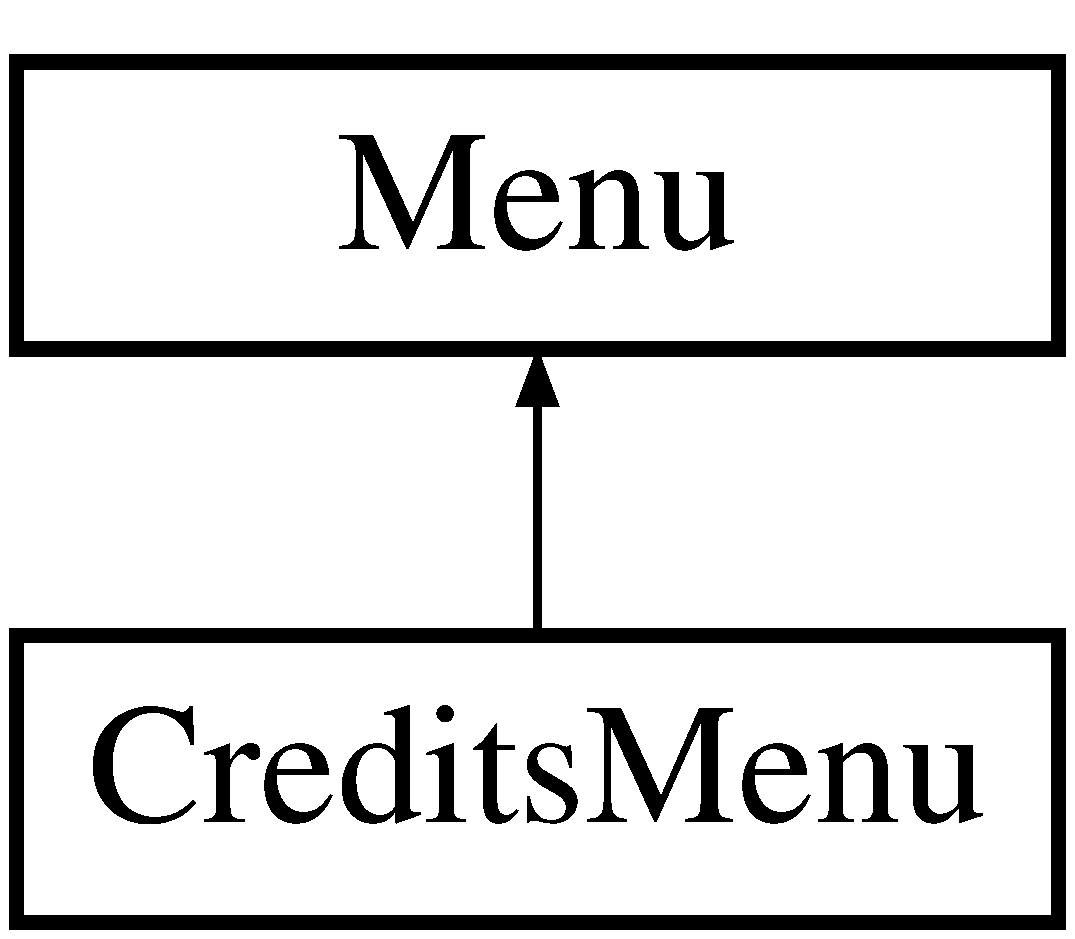
\includegraphics[height=2.000000cm]{class_credits_menu}
\end{center}
\end{figure}
\subsection*{Public Member Functions}
\begin{DoxyCompactItemize}
\item 
\hyperlink{class_credits_menu_a5faefd77a6bf66b98de838e28f1beff1}{Credits\+Menu} ()
\item 
\hyperlink{class_credits_menu_ab044c04c75903dfd5ddc1d1c9e22dc97}{Credits\+Menu} (std\+::string my\+Texture\+Address, sf\+::\+Vector2u my\+Size, sf\+::\+Vector2i my\+Position)
\item 
\hyperlink{class_credits_menu_afab6fd75a71b5faa26508907c28ef3b4}{$\sim$\+Credits\+Menu} ()
\item 
string \hyperlink{class_credits_menu_a7ce3ffb34ef6b1d74a6975506c3f8a92}{get\+Credits\+Address} ()
\item 
sf\+::\+Sprite \hyperlink{class_credits_menu_a285f9f79c86cc255743f70ba7f23e22b}{get\+Sprite} ()
\item 
void \hyperlink{class_credits_menu_ad0d86e63b66e1a68bd6600e59040ff18}{set\+Sprite} (sf\+::\+Sprite)
\item 
void \hyperlink{class_credits_menu_a64fe7f7471ab92c69cbc95cb4ad9dfc8}{draw} (sf\+::\+Render\+Window \&w)
\item 
void \hyperlink{class_credits_menu_afe78658efba17b95a8a7d87d4a90c4d3}{close\+Menu} ()
\item 
void \hyperlink{class_credits_menu_a6fa8421ffafa70e6d6e3af1f61b220c7}{resolve\+Event} (sf\+::\+Event event)
\end{DoxyCompactItemize}
\subsection*{Additional Inherited Members}


\subsection{Constructor \& Destructor Documentation}
\hypertarget{class_credits_menu_a5faefd77a6bf66b98de838e28f1beff1}{\index{Credits\+Menu@{Credits\+Menu}!Credits\+Menu@{Credits\+Menu}}
\index{Credits\+Menu@{Credits\+Menu}!Credits\+Menu@{Credits\+Menu}}
\subsubsection[{Credits\+Menu}]{\setlength{\rightskip}{0pt plus 5cm}Credits\+Menu\+::\+Credits\+Menu (
\begin{DoxyParamCaption}
{}
\end{DoxyParamCaption}
)}}\label{class_credits_menu_a5faefd77a6bf66b98de838e28f1beff1}
\hypertarget{class_credits_menu_ab044c04c75903dfd5ddc1d1c9e22dc97}{\index{Credits\+Menu@{Credits\+Menu}!Credits\+Menu@{Credits\+Menu}}
\index{Credits\+Menu@{Credits\+Menu}!Credits\+Menu@{Credits\+Menu}}
\subsubsection[{Credits\+Menu}]{\setlength{\rightskip}{0pt plus 5cm}Credits\+Menu\+::\+Credits\+Menu (
\begin{DoxyParamCaption}
\item[{std\+::string}]{my\+Texture\+Address, }
\item[{sf\+::\+Vector2u}]{my\+Size, }
\item[{sf\+::\+Vector2i}]{my\+Position}
\end{DoxyParamCaption}
)}}\label{class_credits_menu_ab044c04c75903dfd5ddc1d1c9e22dc97}
\hypertarget{class_credits_menu_afab6fd75a71b5faa26508907c28ef3b4}{\index{Credits\+Menu@{Credits\+Menu}!````~Credits\+Menu@{$\sim$\+Credits\+Menu}}
\index{````~Credits\+Menu@{$\sim$\+Credits\+Menu}!Credits\+Menu@{Credits\+Menu}}
\subsubsection[{$\sim$\+Credits\+Menu}]{\setlength{\rightskip}{0pt plus 5cm}Credits\+Menu\+::$\sim$\+Credits\+Menu (
\begin{DoxyParamCaption}
{}
\end{DoxyParamCaption}
)}}\label{class_credits_menu_afab6fd75a71b5faa26508907c28ef3b4}


\subsection{Member Function Documentation}
\hypertarget{class_credits_menu_afe78658efba17b95a8a7d87d4a90c4d3}{\index{Credits\+Menu@{Credits\+Menu}!close\+Menu@{close\+Menu}}
\index{close\+Menu@{close\+Menu}!Credits\+Menu@{Credits\+Menu}}
\subsubsection[{close\+Menu}]{\setlength{\rightskip}{0pt plus 5cm}void Credits\+Menu\+::close\+Menu (
\begin{DoxyParamCaption}
{}
\end{DoxyParamCaption}
)}}\label{class_credits_menu_afe78658efba17b95a8a7d87d4a90c4d3}
\hypertarget{class_credits_menu_a64fe7f7471ab92c69cbc95cb4ad9dfc8}{\index{Credits\+Menu@{Credits\+Menu}!draw@{draw}}
\index{draw@{draw}!Credits\+Menu@{Credits\+Menu}}
\subsubsection[{draw}]{\setlength{\rightskip}{0pt plus 5cm}void Credits\+Menu\+::draw (
\begin{DoxyParamCaption}
\item[{sf\+::\+Render\+Window \&}]{w}
\end{DoxyParamCaption}
)\hspace{0.3cm}{\ttfamily [virtual]}}}\label{class_credits_menu_a64fe7f7471ab92c69cbc95cb4ad9dfc8}


Reimplemented from \hyperlink{class_menu_a5c486201ec217b10588c145d043e4eb8}{Menu}.

\hypertarget{class_credits_menu_a7ce3ffb34ef6b1d74a6975506c3f8a92}{\index{Credits\+Menu@{Credits\+Menu}!get\+Credits\+Address@{get\+Credits\+Address}}
\index{get\+Credits\+Address@{get\+Credits\+Address}!Credits\+Menu@{Credits\+Menu}}
\subsubsection[{get\+Credits\+Address}]{\setlength{\rightskip}{0pt plus 5cm}string Credits\+Menu\+::get\+Credits\+Address (
\begin{DoxyParamCaption}
{}
\end{DoxyParamCaption}
)}}\label{class_credits_menu_a7ce3ffb34ef6b1d74a6975506c3f8a92}
\hypertarget{class_credits_menu_a285f9f79c86cc255743f70ba7f23e22b}{\index{Credits\+Menu@{Credits\+Menu}!get\+Sprite@{get\+Sprite}}
\index{get\+Sprite@{get\+Sprite}!Credits\+Menu@{Credits\+Menu}}
\subsubsection[{get\+Sprite}]{\setlength{\rightskip}{0pt plus 5cm}sf\+::\+Sprite Credits\+Menu\+::get\+Sprite (
\begin{DoxyParamCaption}
{}
\end{DoxyParamCaption}
)}}\label{class_credits_menu_a285f9f79c86cc255743f70ba7f23e22b}
\hypertarget{class_credits_menu_a6fa8421ffafa70e6d6e3af1f61b220c7}{\index{Credits\+Menu@{Credits\+Menu}!resolve\+Event@{resolve\+Event}}
\index{resolve\+Event@{resolve\+Event}!Credits\+Menu@{Credits\+Menu}}
\subsubsection[{resolve\+Event}]{\setlength{\rightskip}{0pt plus 5cm}void Credits\+Menu\+::resolve\+Event (
\begin{DoxyParamCaption}
\item[{sf\+::\+Event}]{event}
\end{DoxyParamCaption}
)\hspace{0.3cm}{\ttfamily [virtual]}}}\label{class_credits_menu_a6fa8421ffafa70e6d6e3af1f61b220c7}


Implements \hyperlink{class_menu_a91ec4d6d898e740524b1fe3312d8f197}{Menu}.

\hypertarget{class_credits_menu_ad0d86e63b66e1a68bd6600e59040ff18}{\index{Credits\+Menu@{Credits\+Menu}!set\+Sprite@{set\+Sprite}}
\index{set\+Sprite@{set\+Sprite}!Credits\+Menu@{Credits\+Menu}}
\subsubsection[{set\+Sprite}]{\setlength{\rightskip}{0pt plus 5cm}void Credits\+Menu\+::set\+Sprite (
\begin{DoxyParamCaption}
\item[{sf\+::\+Sprite}]{}
\end{DoxyParamCaption}
)}}\label{class_credits_menu_ad0d86e63b66e1a68bd6600e59040ff18}


The documentation for this class was generated from the following files\+:\begin{DoxyCompactItemize}
\item 
D\+:/\+Tower\+Defense/\+Tower\+Defense/\hyperlink{_credits_menu_8h}{Credits\+Menu.\+h}\item 
D\+:/\+Tower\+Defense/\+Tower\+Defense/\hyperlink{_credits_menu_8cpp}{Credits\+Menu.\+cpp}\end{DoxyCompactItemize}

\hypertarget{class_enemy}{\section{Enemy Class Reference}
\label{class_enemy}\index{Enemy@{Enemy}}
}


{\ttfamily \#include $<$Enemy.\+h$>$}

Inheritance diagram for Enemy\+:\begin{figure}[H]
\begin{center}
\leavevmode
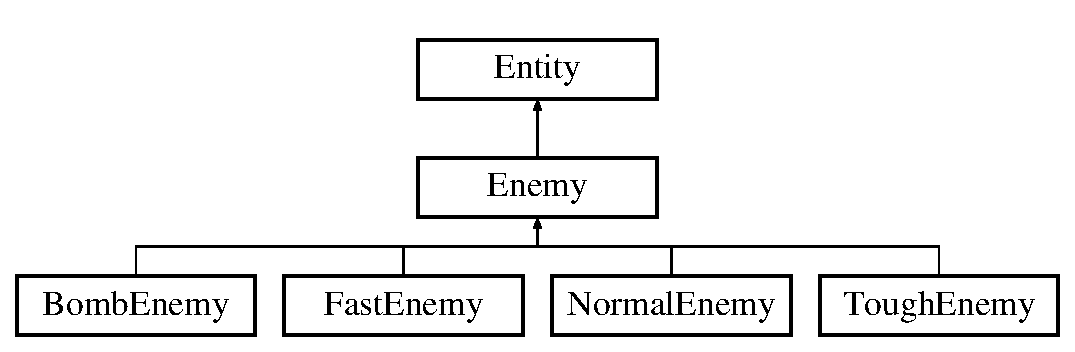
\includegraphics[height=3.000000cm]{class_enemy}
\end{center}
\end{figure}
\subsection*{Public Member Functions}
\begin{DoxyCompactItemize}
\item 
\hyperlink{class_enemy_a94f30d348b6d2840fd71675472ba38dd}{Enemy} ()
\item 
\hyperlink{class_enemy_a54489e1cd1e2fd48465effef7e45fd1b}{Enemy} (int m\+H\+P, float m\+Defence, int m\+Bounty, int m\+Score\+Value, sf\+::\+Sprite m\+Sprite, float m\+Speed)
\item 
virtual \hyperlink{class_enemy_ac0eec4755e28c02688065f9657150ac3}{$\sim$\+Enemy} ()
\item 
virtual bool \hyperlink{class_enemy_a8e0cfa58b8d27e254a0b3c6965962280}{move} ()
\item 
void \hyperlink{class_enemy_a0e46f5b36e6b038bfaef05979bb76325}{succed} ()
\item 
void \hyperlink{class_enemy_a04c451624958712b36546037fc25c601}{die} ()
\item 
void \hyperlink{class_enemy_ad8c2cd506c90a57adad1f94d9e4c25d2}{die\+Without\+Bonus} ()
\item 
void \hyperlink{class_enemy_aa5ddb1dc9aeba11ef0e502527bf6f412}{slow} (int)
\item 
void \hyperlink{class_enemy_a98a78c7c16c3eaca41d60fd54b9ff92a}{un\+Slow} ()
\item 
void \hyperlink{class_enemy_a39d2efd8625d3d8449cc45631d8b4f9b}{update\+Path} ()
\item 
int \hyperlink{class_enemy_ab1c5ecbd2567b509a5d4492764a28f5d}{get\+H\+P} ()
\item 
int \hyperlink{class_enemy_aecdda0124a341bace43f683a766ec6f7}{get\+Bounty} ()
\item 
int \hyperlink{class_enemy_ac04d0b26f6209586b87c8ecbaa0e0257}{get\+Score\+Value} ()
\item 
float \hyperlink{class_enemy_ae01d1b6fedb8f342b7f216ca463d7349}{get\+Defence} ()
\item 
int \hyperlink{class_enemy_af4d6253bc6c28ad1d1ff6deb4303347b}{get\+Slow\+Time} ()
\item 
float \hyperlink{class_enemy_a53020fcba7330809918946e150f8a591}{get\+Distance\+To\+Target} ()
\item 
virtual string \hyperlink{class_enemy_a37b2bae4f5a9e8d673aeb28880ded0bc}{test} ()=0
\item 
void \hyperlink{class_enemy_a0f1e1c58a06fd254c537bf8733e69b63}{set\+Tile} (shared\+\_\+ptr$<$ \hyperlink{class_tile}{Tile} $>$)
\item 
void \hyperlink{class_enemy_a6612d7486e4599d8fbc085c43168962f}{take\+Damage} (int)
\item 
void \hyperlink{class_enemy_ab6302a04e63f97255eb44fc8ce35d012}{draw} (sf\+::\+Render\+Window \&)
\end{DoxyCompactItemize}
\subsection*{Protected Attributes}
\begin{DoxyCompactItemize}
\item 
int \hyperlink{class_enemy_a278d70100af07c946743db1b7a1a9f59}{hp}
\item 
int \hyperlink{class_enemy_ab48bc28310a5ca396fbfaf6edc74996d}{max\+Hp}
\item 
float \hyperlink{class_enemy_a9bb5d74024760e604c41ba79cc7da892}{defence}
\item 
int \hyperlink{class_enemy_a1d9a86d110b87f3cc55b40d1bdb59eb5}{bounty}
\item 
int \hyperlink{class_enemy_abc49d5a2cef917c8ece8a16547f8efee}{score\+Value}
\item 
int \hyperlink{class_enemy_ad59184710c7f9df80138434b8487a9f5}{slow\+Time}
\item 
bool \hyperlink{class_enemy_a7f185bcecfc927871387f6bda2191d0c}{slowed}
\item 
\hyperlink{class_path}{Path} \hyperlink{class_enemy_aff8dab38e3d179a2fb471cf7a9c42cbe}{path}
\end{DoxyCompactItemize}


\subsection{Constructor \& Destructor Documentation}
\hypertarget{class_enemy_a94f30d348b6d2840fd71675472ba38dd}{\index{Enemy@{Enemy}!Enemy@{Enemy}}
\index{Enemy@{Enemy}!Enemy@{Enemy}}
\subsubsection[{Enemy}]{\setlength{\rightskip}{0pt plus 5cm}Enemy\+::\+Enemy (
\begin{DoxyParamCaption}
{}
\end{DoxyParamCaption}
)}}\label{class_enemy_a94f30d348b6d2840fd71675472ba38dd}
\hypertarget{class_enemy_a54489e1cd1e2fd48465effef7e45fd1b}{\index{Enemy@{Enemy}!Enemy@{Enemy}}
\index{Enemy@{Enemy}!Enemy@{Enemy}}
\subsubsection[{Enemy}]{\setlength{\rightskip}{0pt plus 5cm}Enemy\+::\+Enemy (
\begin{DoxyParamCaption}
\item[{int}]{m\+H\+P, }
\item[{float}]{m\+Defence, }
\item[{int}]{m\+Bounty, }
\item[{int}]{m\+Score\+Value, }
\item[{sf\+::\+Sprite}]{m\+Sprite, }
\item[{float}]{m\+Speed}
\end{DoxyParamCaption}
)}}\label{class_enemy_a54489e1cd1e2fd48465effef7e45fd1b}
\hypertarget{class_enemy_ac0eec4755e28c02688065f9657150ac3}{\index{Enemy@{Enemy}!````~Enemy@{$\sim$\+Enemy}}
\index{````~Enemy@{$\sim$\+Enemy}!Enemy@{Enemy}}
\subsubsection[{$\sim$\+Enemy}]{\setlength{\rightskip}{0pt plus 5cm}Enemy\+::$\sim$\+Enemy (
\begin{DoxyParamCaption}
{}
\end{DoxyParamCaption}
)\hspace{0.3cm}{\ttfamily [virtual]}}}\label{class_enemy_ac0eec4755e28c02688065f9657150ac3}


\subsection{Member Function Documentation}
\hypertarget{class_enemy_a04c451624958712b36546037fc25c601}{\index{Enemy@{Enemy}!die@{die}}
\index{die@{die}!Enemy@{Enemy}}
\subsubsection[{die}]{\setlength{\rightskip}{0pt plus 5cm}void Enemy\+::die (
\begin{DoxyParamCaption}
{}
\end{DoxyParamCaption}
)}}\label{class_enemy_a04c451624958712b36546037fc25c601}
\hypertarget{class_enemy_ad8c2cd506c90a57adad1f94d9e4c25d2}{\index{Enemy@{Enemy}!die\+Without\+Bonus@{die\+Without\+Bonus}}
\index{die\+Without\+Bonus@{die\+Without\+Bonus}!Enemy@{Enemy}}
\subsubsection[{die\+Without\+Bonus}]{\setlength{\rightskip}{0pt plus 5cm}void Enemy\+::die\+Without\+Bonus (
\begin{DoxyParamCaption}
{}
\end{DoxyParamCaption}
)}}\label{class_enemy_ad8c2cd506c90a57adad1f94d9e4c25d2}
\hypertarget{class_enemy_ab6302a04e63f97255eb44fc8ce35d012}{\index{Enemy@{Enemy}!draw@{draw}}
\index{draw@{draw}!Enemy@{Enemy}}
\subsubsection[{draw}]{\setlength{\rightskip}{0pt plus 5cm}void Enemy\+::draw (
\begin{DoxyParamCaption}
\item[{sf\+::\+Render\+Window \&}]{w}
\end{DoxyParamCaption}
)\hspace{0.3cm}{\ttfamily [virtual]}}}\label{class_enemy_ab6302a04e63f97255eb44fc8ce35d012}


Reimplemented from \hyperlink{class_entity_a0eca969d39e7b7bc728236f85e02bbb6}{Entity}.

\hypertarget{class_enemy_aecdda0124a341bace43f683a766ec6f7}{\index{Enemy@{Enemy}!get\+Bounty@{get\+Bounty}}
\index{get\+Bounty@{get\+Bounty}!Enemy@{Enemy}}
\subsubsection[{get\+Bounty}]{\setlength{\rightskip}{0pt plus 5cm}int Enemy\+::get\+Bounty (
\begin{DoxyParamCaption}
{}
\end{DoxyParamCaption}
)}}\label{class_enemy_aecdda0124a341bace43f683a766ec6f7}
\hypertarget{class_enemy_ae01d1b6fedb8f342b7f216ca463d7349}{\index{Enemy@{Enemy}!get\+Defence@{get\+Defence}}
\index{get\+Defence@{get\+Defence}!Enemy@{Enemy}}
\subsubsection[{get\+Defence}]{\setlength{\rightskip}{0pt plus 5cm}float Enemy\+::get\+Defence (
\begin{DoxyParamCaption}
{}
\end{DoxyParamCaption}
)}}\label{class_enemy_ae01d1b6fedb8f342b7f216ca463d7349}
\hypertarget{class_enemy_a53020fcba7330809918946e150f8a591}{\index{Enemy@{Enemy}!get\+Distance\+To\+Target@{get\+Distance\+To\+Target}}
\index{get\+Distance\+To\+Target@{get\+Distance\+To\+Target}!Enemy@{Enemy}}
\subsubsection[{get\+Distance\+To\+Target}]{\setlength{\rightskip}{0pt plus 5cm}float Enemy\+::get\+Distance\+To\+Target (
\begin{DoxyParamCaption}
{}
\end{DoxyParamCaption}
)}}\label{class_enemy_a53020fcba7330809918946e150f8a591}
\hypertarget{class_enemy_ab1c5ecbd2567b509a5d4492764a28f5d}{\index{Enemy@{Enemy}!get\+H\+P@{get\+H\+P}}
\index{get\+H\+P@{get\+H\+P}!Enemy@{Enemy}}
\subsubsection[{get\+H\+P}]{\setlength{\rightskip}{0pt plus 5cm}int Enemy\+::get\+H\+P (
\begin{DoxyParamCaption}
{}
\end{DoxyParamCaption}
)}}\label{class_enemy_ab1c5ecbd2567b509a5d4492764a28f5d}
\hypertarget{class_enemy_ac04d0b26f6209586b87c8ecbaa0e0257}{\index{Enemy@{Enemy}!get\+Score\+Value@{get\+Score\+Value}}
\index{get\+Score\+Value@{get\+Score\+Value}!Enemy@{Enemy}}
\subsubsection[{get\+Score\+Value}]{\setlength{\rightskip}{0pt plus 5cm}int Enemy\+::get\+Score\+Value (
\begin{DoxyParamCaption}
{}
\end{DoxyParamCaption}
)}}\label{class_enemy_ac04d0b26f6209586b87c8ecbaa0e0257}
\hypertarget{class_enemy_af4d6253bc6c28ad1d1ff6deb4303347b}{\index{Enemy@{Enemy}!get\+Slow\+Time@{get\+Slow\+Time}}
\index{get\+Slow\+Time@{get\+Slow\+Time}!Enemy@{Enemy}}
\subsubsection[{get\+Slow\+Time}]{\setlength{\rightskip}{0pt plus 5cm}int Enemy\+::get\+Slow\+Time (
\begin{DoxyParamCaption}
{}
\end{DoxyParamCaption}
)}}\label{class_enemy_af4d6253bc6c28ad1d1ff6deb4303347b}
\hypertarget{class_enemy_a8e0cfa58b8d27e254a0b3c6965962280}{\index{Enemy@{Enemy}!move@{move}}
\index{move@{move}!Enemy@{Enemy}}
\subsubsection[{move}]{\setlength{\rightskip}{0pt plus 5cm}bool Enemy\+::move (
\begin{DoxyParamCaption}
{}
\end{DoxyParamCaption}
)\hspace{0.3cm}{\ttfamily [virtual]}}}\label{class_enemy_a8e0cfa58b8d27e254a0b3c6965962280}


Reimplemented in \hyperlink{class_bomb_enemy_ae421414fdc87d4cb92bdc6975a3b28b4}{Bomb\+Enemy}.

\hypertarget{class_enemy_a0f1e1c58a06fd254c537bf8733e69b63}{\index{Enemy@{Enemy}!set\+Tile@{set\+Tile}}
\index{set\+Tile@{set\+Tile}!Enemy@{Enemy}}
\subsubsection[{set\+Tile}]{\setlength{\rightskip}{0pt plus 5cm}void Enemy\+::set\+Tile (
\begin{DoxyParamCaption}
\item[{shared\+\_\+ptr$<$ {\bf Tile} $>$}]{t}
\end{DoxyParamCaption}
)}}\label{class_enemy_a0f1e1c58a06fd254c537bf8733e69b63}
\hypertarget{class_enemy_aa5ddb1dc9aeba11ef0e502527bf6f412}{\index{Enemy@{Enemy}!slow@{slow}}
\index{slow@{slow}!Enemy@{Enemy}}
\subsubsection[{slow}]{\setlength{\rightskip}{0pt plus 5cm}void Enemy\+::slow (
\begin{DoxyParamCaption}
\item[{int}]{frames}
\end{DoxyParamCaption}
)}}\label{class_enemy_aa5ddb1dc9aeba11ef0e502527bf6f412}
\hypertarget{class_enemy_a0e46f5b36e6b038bfaef05979bb76325}{\index{Enemy@{Enemy}!succed@{succed}}
\index{succed@{succed}!Enemy@{Enemy}}
\subsubsection[{succed}]{\setlength{\rightskip}{0pt plus 5cm}void Enemy\+::succed (
\begin{DoxyParamCaption}
{}
\end{DoxyParamCaption}
)}}\label{class_enemy_a0e46f5b36e6b038bfaef05979bb76325}
\hypertarget{class_enemy_a6612d7486e4599d8fbc085c43168962f}{\index{Enemy@{Enemy}!take\+Damage@{take\+Damage}}
\index{take\+Damage@{take\+Damage}!Enemy@{Enemy}}
\subsubsection[{take\+Damage}]{\setlength{\rightskip}{0pt plus 5cm}void Enemy\+::take\+Damage (
\begin{DoxyParamCaption}
\item[{int}]{damage}
\end{DoxyParamCaption}
)}}\label{class_enemy_a6612d7486e4599d8fbc085c43168962f}
\hypertarget{class_enemy_a37b2bae4f5a9e8d673aeb28880ded0bc}{\index{Enemy@{Enemy}!test@{test}}
\index{test@{test}!Enemy@{Enemy}}
\subsubsection[{test}]{\setlength{\rightskip}{0pt plus 5cm}virtual string Enemy\+::test (
\begin{DoxyParamCaption}
{}
\end{DoxyParamCaption}
)\hspace{0.3cm}{\ttfamily [pure virtual]}}}\label{class_enemy_a37b2bae4f5a9e8d673aeb28880ded0bc}


Implemented in \hyperlink{class_bomb_enemy_a6fde389b791b1d977caa01a15a66df1c}{Bomb\+Enemy}, \hyperlink{class_fast_enemy_ab6e1d144ceda128e4b2717a82a570b51}{Fast\+Enemy}, \hyperlink{class_normal_enemy_a3409e903bc18e9ab9d58d8181ec6658f}{Normal\+Enemy}, and \hyperlink{class_tough_enemy_aec2e1a119c04896b1bd5aa7b36e2acca}{Tough\+Enemy}.

\hypertarget{class_enemy_a98a78c7c16c3eaca41d60fd54b9ff92a}{\index{Enemy@{Enemy}!un\+Slow@{un\+Slow}}
\index{un\+Slow@{un\+Slow}!Enemy@{Enemy}}
\subsubsection[{un\+Slow}]{\setlength{\rightskip}{0pt plus 5cm}void Enemy\+::un\+Slow (
\begin{DoxyParamCaption}
{}
\end{DoxyParamCaption}
)}}\label{class_enemy_a98a78c7c16c3eaca41d60fd54b9ff92a}
\hypertarget{class_enemy_a39d2efd8625d3d8449cc45631d8b4f9b}{\index{Enemy@{Enemy}!update\+Path@{update\+Path}}
\index{update\+Path@{update\+Path}!Enemy@{Enemy}}
\subsubsection[{update\+Path}]{\setlength{\rightskip}{0pt plus 5cm}void Enemy\+::update\+Path (
\begin{DoxyParamCaption}
{}
\end{DoxyParamCaption}
)}}\label{class_enemy_a39d2efd8625d3d8449cc45631d8b4f9b}


\subsection{Member Data Documentation}
\hypertarget{class_enemy_a1d9a86d110b87f3cc55b40d1bdb59eb5}{\index{Enemy@{Enemy}!bounty@{bounty}}
\index{bounty@{bounty}!Enemy@{Enemy}}
\subsubsection[{bounty}]{\setlength{\rightskip}{0pt plus 5cm}int Enemy\+::bounty\hspace{0.3cm}{\ttfamily [protected]}}}\label{class_enemy_a1d9a86d110b87f3cc55b40d1bdb59eb5}
\hypertarget{class_enemy_a9bb5d74024760e604c41ba79cc7da892}{\index{Enemy@{Enemy}!defence@{defence}}
\index{defence@{defence}!Enemy@{Enemy}}
\subsubsection[{defence}]{\setlength{\rightskip}{0pt plus 5cm}float Enemy\+::defence\hspace{0.3cm}{\ttfamily [protected]}}}\label{class_enemy_a9bb5d74024760e604c41ba79cc7da892}
\hypertarget{class_enemy_a278d70100af07c946743db1b7a1a9f59}{\index{Enemy@{Enemy}!hp@{hp}}
\index{hp@{hp}!Enemy@{Enemy}}
\subsubsection[{hp}]{\setlength{\rightskip}{0pt plus 5cm}int Enemy\+::hp\hspace{0.3cm}{\ttfamily [protected]}}}\label{class_enemy_a278d70100af07c946743db1b7a1a9f59}
\hypertarget{class_enemy_ab48bc28310a5ca396fbfaf6edc74996d}{\index{Enemy@{Enemy}!max\+Hp@{max\+Hp}}
\index{max\+Hp@{max\+Hp}!Enemy@{Enemy}}
\subsubsection[{max\+Hp}]{\setlength{\rightskip}{0pt plus 5cm}int Enemy\+::max\+Hp\hspace{0.3cm}{\ttfamily [protected]}}}\label{class_enemy_ab48bc28310a5ca396fbfaf6edc74996d}
\hypertarget{class_enemy_aff8dab38e3d179a2fb471cf7a9c42cbe}{\index{Enemy@{Enemy}!path@{path}}
\index{path@{path}!Enemy@{Enemy}}
\subsubsection[{path}]{\setlength{\rightskip}{0pt plus 5cm}{\bf Path} Enemy\+::path\hspace{0.3cm}{\ttfamily [protected]}}}\label{class_enemy_aff8dab38e3d179a2fb471cf7a9c42cbe}
\hypertarget{class_enemy_abc49d5a2cef917c8ece8a16547f8efee}{\index{Enemy@{Enemy}!score\+Value@{score\+Value}}
\index{score\+Value@{score\+Value}!Enemy@{Enemy}}
\subsubsection[{score\+Value}]{\setlength{\rightskip}{0pt plus 5cm}int Enemy\+::score\+Value\hspace{0.3cm}{\ttfamily [protected]}}}\label{class_enemy_abc49d5a2cef917c8ece8a16547f8efee}
\hypertarget{class_enemy_a7f185bcecfc927871387f6bda2191d0c}{\index{Enemy@{Enemy}!slowed@{slowed}}
\index{slowed@{slowed}!Enemy@{Enemy}}
\subsubsection[{slowed}]{\setlength{\rightskip}{0pt plus 5cm}bool Enemy\+::slowed\hspace{0.3cm}{\ttfamily [protected]}}}\label{class_enemy_a7f185bcecfc927871387f6bda2191d0c}
\hypertarget{class_enemy_ad59184710c7f9df80138434b8487a9f5}{\index{Enemy@{Enemy}!slow\+Time@{slow\+Time}}
\index{slow\+Time@{slow\+Time}!Enemy@{Enemy}}
\subsubsection[{slow\+Time}]{\setlength{\rightskip}{0pt plus 5cm}int Enemy\+::slow\+Time\hspace{0.3cm}{\ttfamily [protected]}}}\label{class_enemy_ad59184710c7f9df80138434b8487a9f5}


The documentation for this class was generated from the following files\+:\begin{DoxyCompactItemize}
\item 
D\+:/\+Tower\+Defense/\+Tower\+Defense/\hyperlink{_enemy_8h}{Enemy.\+h}\item 
D\+:/\+Tower\+Defense/\+Tower\+Defense/\hyperlink{_enemy_8cpp}{Enemy.\+cpp}\end{DoxyCompactItemize}

\hypertarget{class_entity}{\section{Entity Class Reference}
\label{class_entity}\index{Entity@{Entity}}
}


{\ttfamily \#include $<$Entity.\+h$>$}

Inheritance diagram for Entity\+:\begin{figure}[H]
\begin{center}
\leavevmode
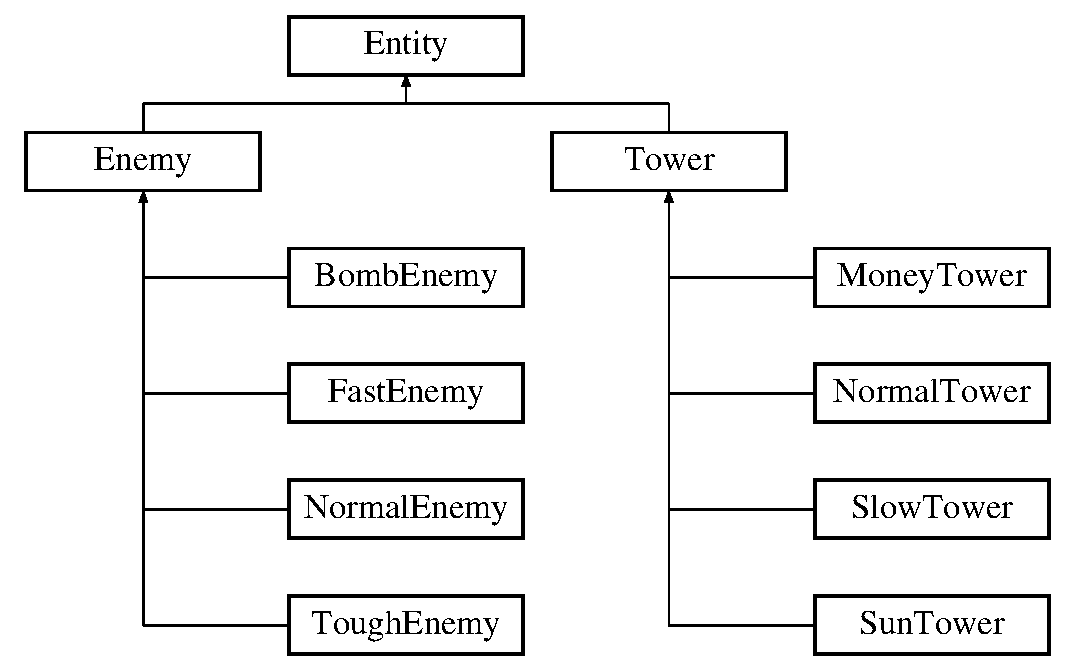
\includegraphics[height=6.000000cm]{class_entity}
\end{center}
\end{figure}
\subsection*{Public Member Functions}
\begin{DoxyCompactItemize}
\item 
\hyperlink{class_entity_a980f368aa07ce358583982821533a54a}{Entity} ()
\item 
virtual \hyperlink{class_entity_adf6d3f7cb1b2ba029b6b048a395cc8ae}{$\sim$\+Entity} ()
\item 
sf\+::\+Vector2i \hyperlink{class_entity_a1bc281383bd777ba96dd0c7c989ba1e7}{get\+Position} ()
\item 
sf\+::\+Vector2i \hyperlink{class_entity_aad4cbcdad1ba43221eff4e5474dfdd58}{get\+Size} ()
\item 
float \hyperlink{class_entity_a1ab1df6a898303e678a11d727016dd09}{get\+Speed} ()
\item 
sf\+::\+Sprite \hyperlink{class_entity_aa5dd2cfe8cd0bd31e908752bf7c4b510}{get\+Sprite} ()
\item 
shared\+\_\+ptr$<$ \hyperlink{class_tile}{Tile} $>$ \hyperlink{class_entity_a4c0e3e14381db594a39b0b1fa69b9bc7}{get\+Tile} ()
\item 
void \hyperlink{class_entity_a999e10122f45fb582c2d4976f12e4c3e}{set\+Position} (sf\+::\+Vector2i m\+Position)
\item 
void \hyperlink{class_entity_a5d01a1d6f13fa685d75ac657d2e72b6b}{set\+Size} (sf\+::\+Vector2i m\+Size)
\item 
void \hyperlink{class_entity_a752b7fb05557c905dcdce931500e700e}{set\+Speed} (float m\+Speed)
\item 
void \hyperlink{class_entity_acffd8697cae92e62b0962c78e2d45d06}{set\+Sprite} (sf\+::\+Sprite m\+Sprite)
\item 
virtual void \hyperlink{class_entity_a0eca969d39e7b7bc728236f85e02bbb6}{draw} (sf\+::\+Render\+Window \&)
\end{DoxyCompactItemize}
\subsection*{Protected Attributes}
\begin{DoxyCompactItemize}
\item 
sf\+::\+Vector2i \hyperlink{class_entity_aa58364f83a24774ad8d29e2f5e48e06d}{position}
\item 
sf\+::\+Vector2i \hyperlink{class_entity_ae32cdf24e4f89bee02c7132c4d6e9c18}{size}
\item 
float \hyperlink{class_entity_a1de3d8d9ab8088f61e6726069b26fa60}{speed}
\item 
sf\+::\+Sprite \hyperlink{class_entity_a48ef4ab143b8d0211877c9f6be42e824}{sprite}
\item 
shared\+\_\+ptr$<$ \hyperlink{class_tile}{Tile} $>$ \hyperlink{class_entity_a2774f1e938416fab37040a33ec573495}{tile}
\item 
int \hyperlink{class_entity_abccceab981ceb2c361408358a6ff0585}{timer}
\item 
sf\+::\+Texture \hyperlink{class_entity_ad64dd6d282432a68475f30f7c7bbdc88}{texture}
\end{DoxyCompactItemize}


\subsection{Constructor \& Destructor Documentation}
\hypertarget{class_entity_a980f368aa07ce358583982821533a54a}{\index{Entity@{Entity}!Entity@{Entity}}
\index{Entity@{Entity}!Entity@{Entity}}
\subsubsection[{Entity}]{\setlength{\rightskip}{0pt plus 5cm}Entity\+::\+Entity (
\begin{DoxyParamCaption}
{}
\end{DoxyParamCaption}
)}}\label{class_entity_a980f368aa07ce358583982821533a54a}
\hypertarget{class_entity_adf6d3f7cb1b2ba029b6b048a395cc8ae}{\index{Entity@{Entity}!````~Entity@{$\sim$\+Entity}}
\index{````~Entity@{$\sim$\+Entity}!Entity@{Entity}}
\subsubsection[{$\sim$\+Entity}]{\setlength{\rightskip}{0pt plus 5cm}Entity\+::$\sim$\+Entity (
\begin{DoxyParamCaption}
{}
\end{DoxyParamCaption}
)\hspace{0.3cm}{\ttfamily [virtual]}}}\label{class_entity_adf6d3f7cb1b2ba029b6b048a395cc8ae}


\subsection{Member Function Documentation}
\hypertarget{class_entity_a0eca969d39e7b7bc728236f85e02bbb6}{\index{Entity@{Entity}!draw@{draw}}
\index{draw@{draw}!Entity@{Entity}}
\subsubsection[{draw}]{\setlength{\rightskip}{0pt plus 5cm}void Entity\+::draw (
\begin{DoxyParamCaption}
\item[{sf\+::\+Render\+Window \&}]{w}
\end{DoxyParamCaption}
)\hspace{0.3cm}{\ttfamily [virtual]}}}\label{class_entity_a0eca969d39e7b7bc728236f85e02bbb6}


Reimplemented in \hyperlink{class_enemy_ab6302a04e63f97255eb44fc8ce35d012}{Enemy}.

\hypertarget{class_entity_a1bc281383bd777ba96dd0c7c989ba1e7}{\index{Entity@{Entity}!get\+Position@{get\+Position}}
\index{get\+Position@{get\+Position}!Entity@{Entity}}
\subsubsection[{get\+Position}]{\setlength{\rightskip}{0pt plus 5cm}sf\+::\+Vector2i Entity\+::get\+Position (
\begin{DoxyParamCaption}
{}
\end{DoxyParamCaption}
)}}\label{class_entity_a1bc281383bd777ba96dd0c7c989ba1e7}
\hypertarget{class_entity_aad4cbcdad1ba43221eff4e5474dfdd58}{\index{Entity@{Entity}!get\+Size@{get\+Size}}
\index{get\+Size@{get\+Size}!Entity@{Entity}}
\subsubsection[{get\+Size}]{\setlength{\rightskip}{0pt plus 5cm}sf\+::\+Vector2i Entity\+::get\+Size (
\begin{DoxyParamCaption}
{}
\end{DoxyParamCaption}
)}}\label{class_entity_aad4cbcdad1ba43221eff4e5474dfdd58}
\hypertarget{class_entity_a1ab1df6a898303e678a11d727016dd09}{\index{Entity@{Entity}!get\+Speed@{get\+Speed}}
\index{get\+Speed@{get\+Speed}!Entity@{Entity}}
\subsubsection[{get\+Speed}]{\setlength{\rightskip}{0pt plus 5cm}float Entity\+::get\+Speed (
\begin{DoxyParamCaption}
{}
\end{DoxyParamCaption}
)}}\label{class_entity_a1ab1df6a898303e678a11d727016dd09}
\hypertarget{class_entity_aa5dd2cfe8cd0bd31e908752bf7c4b510}{\index{Entity@{Entity}!get\+Sprite@{get\+Sprite}}
\index{get\+Sprite@{get\+Sprite}!Entity@{Entity}}
\subsubsection[{get\+Sprite}]{\setlength{\rightskip}{0pt plus 5cm}sf\+::\+Sprite Entity\+::get\+Sprite (
\begin{DoxyParamCaption}
{}
\end{DoxyParamCaption}
)}}\label{class_entity_aa5dd2cfe8cd0bd31e908752bf7c4b510}
\hypertarget{class_entity_a4c0e3e14381db594a39b0b1fa69b9bc7}{\index{Entity@{Entity}!get\+Tile@{get\+Tile}}
\index{get\+Tile@{get\+Tile}!Entity@{Entity}}
\subsubsection[{get\+Tile}]{\setlength{\rightskip}{0pt plus 5cm}shared\+\_\+ptr$<$ {\bf Tile} $>$ Entity\+::get\+Tile (
\begin{DoxyParamCaption}
{}
\end{DoxyParamCaption}
)}}\label{class_entity_a4c0e3e14381db594a39b0b1fa69b9bc7}
\hypertarget{class_entity_a999e10122f45fb582c2d4976f12e4c3e}{\index{Entity@{Entity}!set\+Position@{set\+Position}}
\index{set\+Position@{set\+Position}!Entity@{Entity}}
\subsubsection[{set\+Position}]{\setlength{\rightskip}{0pt plus 5cm}void Entity\+::set\+Position (
\begin{DoxyParamCaption}
\item[{sf\+::\+Vector2i}]{m\+Position}
\end{DoxyParamCaption}
)}}\label{class_entity_a999e10122f45fb582c2d4976f12e4c3e}
\hypertarget{class_entity_a5d01a1d6f13fa685d75ac657d2e72b6b}{\index{Entity@{Entity}!set\+Size@{set\+Size}}
\index{set\+Size@{set\+Size}!Entity@{Entity}}
\subsubsection[{set\+Size}]{\setlength{\rightskip}{0pt plus 5cm}void Entity\+::set\+Size (
\begin{DoxyParamCaption}
\item[{sf\+::\+Vector2i}]{m\+Size}
\end{DoxyParamCaption}
)}}\label{class_entity_a5d01a1d6f13fa685d75ac657d2e72b6b}
\hypertarget{class_entity_a752b7fb05557c905dcdce931500e700e}{\index{Entity@{Entity}!set\+Speed@{set\+Speed}}
\index{set\+Speed@{set\+Speed}!Entity@{Entity}}
\subsubsection[{set\+Speed}]{\setlength{\rightskip}{0pt plus 5cm}void Entity\+::set\+Speed (
\begin{DoxyParamCaption}
\item[{float}]{m\+Speed}
\end{DoxyParamCaption}
)}}\label{class_entity_a752b7fb05557c905dcdce931500e700e}
\hypertarget{class_entity_acffd8697cae92e62b0962c78e2d45d06}{\index{Entity@{Entity}!set\+Sprite@{set\+Sprite}}
\index{set\+Sprite@{set\+Sprite}!Entity@{Entity}}
\subsubsection[{set\+Sprite}]{\setlength{\rightskip}{0pt plus 5cm}void Entity\+::set\+Sprite (
\begin{DoxyParamCaption}
\item[{sf\+::\+Sprite}]{m\+Sprite}
\end{DoxyParamCaption}
)}}\label{class_entity_acffd8697cae92e62b0962c78e2d45d06}


\subsection{Member Data Documentation}
\hypertarget{class_entity_aa58364f83a24774ad8d29e2f5e48e06d}{\index{Entity@{Entity}!position@{position}}
\index{position@{position}!Entity@{Entity}}
\subsubsection[{position}]{\setlength{\rightskip}{0pt plus 5cm}sf\+::\+Vector2i Entity\+::position\hspace{0.3cm}{\ttfamily [protected]}}}\label{class_entity_aa58364f83a24774ad8d29e2f5e48e06d}
\hypertarget{class_entity_ae32cdf24e4f89bee02c7132c4d6e9c18}{\index{Entity@{Entity}!size@{size}}
\index{size@{size}!Entity@{Entity}}
\subsubsection[{size}]{\setlength{\rightskip}{0pt plus 5cm}sf\+::\+Vector2i Entity\+::size\hspace{0.3cm}{\ttfamily [protected]}}}\label{class_entity_ae32cdf24e4f89bee02c7132c4d6e9c18}
\hypertarget{class_entity_a1de3d8d9ab8088f61e6726069b26fa60}{\index{Entity@{Entity}!speed@{speed}}
\index{speed@{speed}!Entity@{Entity}}
\subsubsection[{speed}]{\setlength{\rightskip}{0pt plus 5cm}float Entity\+::speed\hspace{0.3cm}{\ttfamily [protected]}}}\label{class_entity_a1de3d8d9ab8088f61e6726069b26fa60}
\hypertarget{class_entity_a48ef4ab143b8d0211877c9f6be42e824}{\index{Entity@{Entity}!sprite@{sprite}}
\index{sprite@{sprite}!Entity@{Entity}}
\subsubsection[{sprite}]{\setlength{\rightskip}{0pt plus 5cm}sf\+::\+Sprite Entity\+::sprite\hspace{0.3cm}{\ttfamily [protected]}}}\label{class_entity_a48ef4ab143b8d0211877c9f6be42e824}
\hypertarget{class_entity_ad64dd6d282432a68475f30f7c7bbdc88}{\index{Entity@{Entity}!texture@{texture}}
\index{texture@{texture}!Entity@{Entity}}
\subsubsection[{texture}]{\setlength{\rightskip}{0pt plus 5cm}sf\+::\+Texture Entity\+::texture\hspace{0.3cm}{\ttfamily [protected]}}}\label{class_entity_ad64dd6d282432a68475f30f7c7bbdc88}
\hypertarget{class_entity_a2774f1e938416fab37040a33ec573495}{\index{Entity@{Entity}!tile@{tile}}
\index{tile@{tile}!Entity@{Entity}}
\subsubsection[{tile}]{\setlength{\rightskip}{0pt plus 5cm}shared\+\_\+ptr$<${\bf Tile}$>$ Entity\+::tile\hspace{0.3cm}{\ttfamily [protected]}}}\label{class_entity_a2774f1e938416fab37040a33ec573495}
\hypertarget{class_entity_abccceab981ceb2c361408358a6ff0585}{\index{Entity@{Entity}!timer@{timer}}
\index{timer@{timer}!Entity@{Entity}}
\subsubsection[{timer}]{\setlength{\rightskip}{0pt plus 5cm}int Entity\+::timer\hspace{0.3cm}{\ttfamily [protected]}}}\label{class_entity_abccceab981ceb2c361408358a6ff0585}


The documentation for this class was generated from the following files\+:\begin{DoxyCompactItemize}
\item 
D\+:/\+Tower\+Defense/\+Tower\+Defense/\hyperlink{_entity_8h}{Entity.\+h}\item 
D\+:/\+Tower\+Defense/\+Tower\+Defense/\hyperlink{_entity_8cpp}{Entity.\+cpp}\end{DoxyCompactItemize}

\hypertarget{class_fast_enemy}{\section{Fast\+Enemy Class Reference}
\label{class_fast_enemy}\index{Fast\+Enemy@{Fast\+Enemy}}
}


{\ttfamily \#include $<$Fast\+Enemy.\+h$>$}

Inheritance diagram for Fast\+Enemy\+:\begin{figure}[H]
\begin{center}
\leavevmode
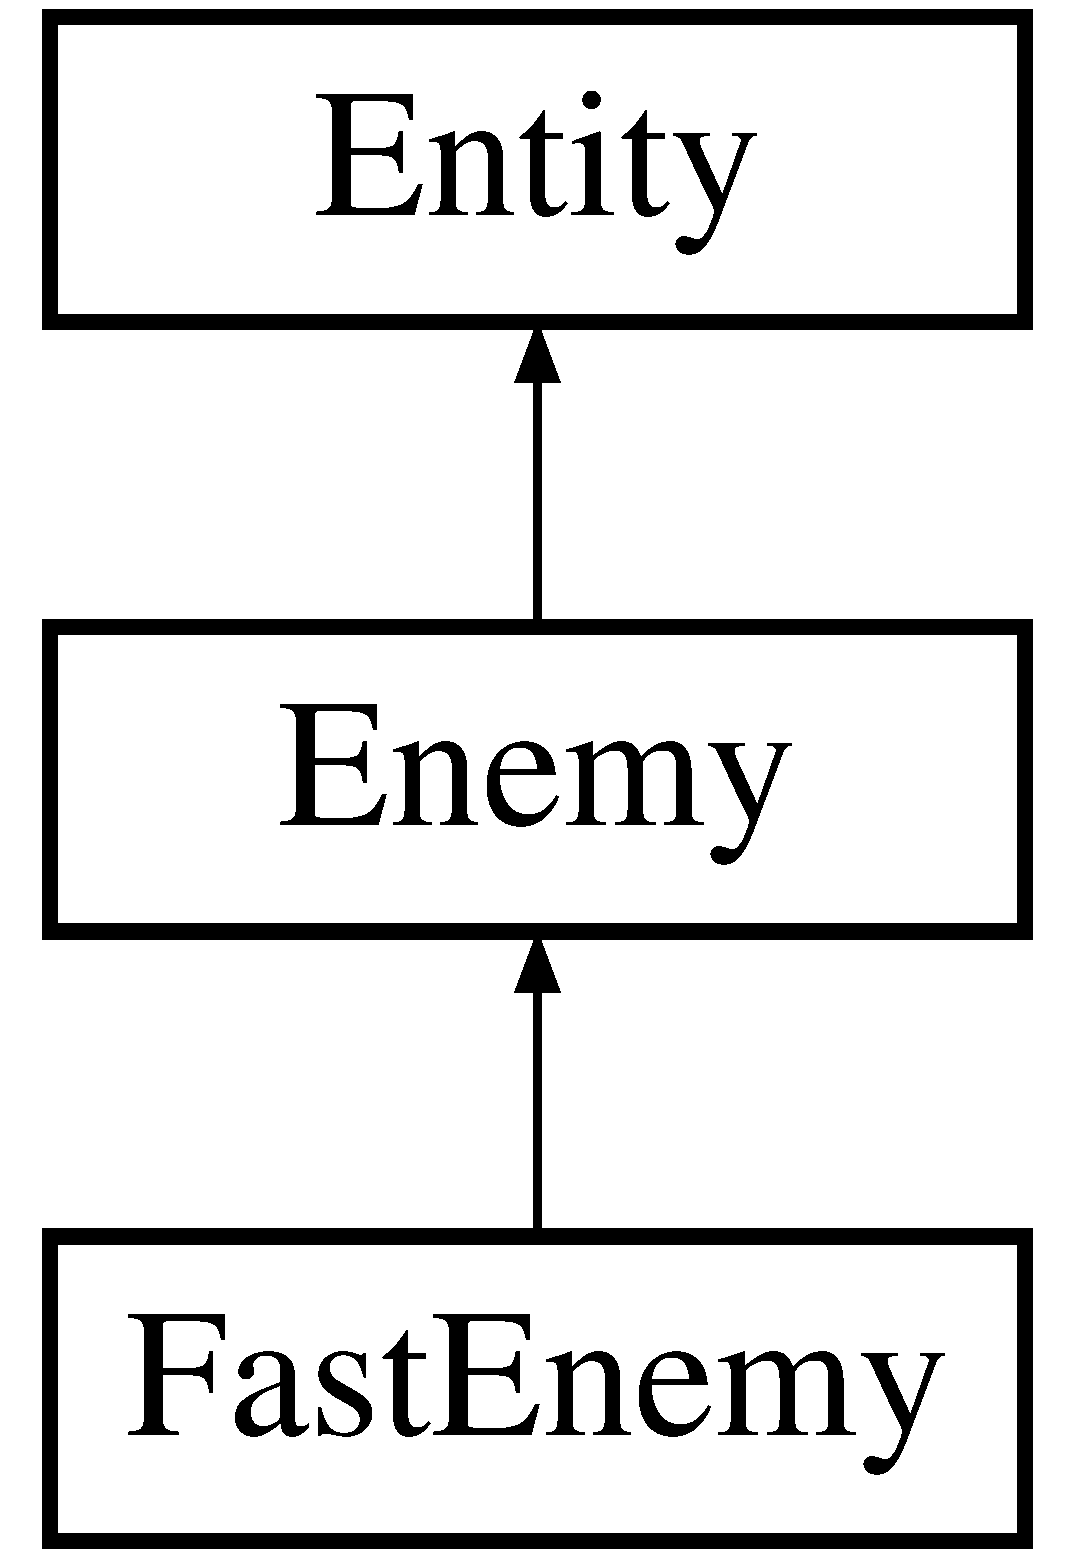
\includegraphics[height=3.000000cm]{class_fast_enemy}
\end{center}
\end{figure}
\subsection*{Public Member Functions}
\begin{DoxyCompactItemize}
\item 
\hyperlink{class_fast_enemy_a22193a351c1600aa27a754dd1e98f828}{Fast\+Enemy} ()
\item 
\hyperlink{class_fast_enemy_a385d3a2fd3a4b83bfb0a9820ae5a9905}{Fast\+Enemy} (int \hyperlink{class_enemy_a278d70100af07c946743db1b7a1a9f59}{hp}, float \hyperlink{class_enemy_a9bb5d74024760e604c41ba79cc7da892}{defence}, int \hyperlink{class_enemy_a1d9a86d110b87f3cc55b40d1bdb59eb5}{bounty}, int \hyperlink{class_enemy_abc49d5a2cef917c8ece8a16547f8efee}{score\+Value}, sf\+::\+Sprite \hyperlink{class_entity_a48ef4ab143b8d0211877c9f6be42e824}{sprite}, float \hyperlink{class_entity_a1de3d8d9ab8088f61e6726069b26fa60}{speed})
\item 
virtual \hyperlink{class_fast_enemy_a40b6cd76a5b3d4339129b912b24ec353}{$\sim$\+Fast\+Enemy} ()
\item 
string \hyperlink{class_fast_enemy_ab6e1d144ceda128e4b2717a82a570b51}{test} ()
\end{DoxyCompactItemize}
\subsection*{Additional Inherited Members}


\subsection{Constructor \& Destructor Documentation}
\hypertarget{class_fast_enemy_a22193a351c1600aa27a754dd1e98f828}{\index{Fast\+Enemy@{Fast\+Enemy}!Fast\+Enemy@{Fast\+Enemy}}
\index{Fast\+Enemy@{Fast\+Enemy}!Fast\+Enemy@{Fast\+Enemy}}
\subsubsection[{Fast\+Enemy}]{\setlength{\rightskip}{0pt plus 5cm}Fast\+Enemy\+::\+Fast\+Enemy (
\begin{DoxyParamCaption}
{}
\end{DoxyParamCaption}
)}}\label{class_fast_enemy_a22193a351c1600aa27a754dd1e98f828}
\hypertarget{class_fast_enemy_a385d3a2fd3a4b83bfb0a9820ae5a9905}{\index{Fast\+Enemy@{Fast\+Enemy}!Fast\+Enemy@{Fast\+Enemy}}
\index{Fast\+Enemy@{Fast\+Enemy}!Fast\+Enemy@{Fast\+Enemy}}
\subsubsection[{Fast\+Enemy}]{\setlength{\rightskip}{0pt plus 5cm}Fast\+Enemy\+::\+Fast\+Enemy (
\begin{DoxyParamCaption}
\item[{int}]{hp, }
\item[{float}]{defence, }
\item[{int}]{bounty, }
\item[{int}]{score\+Value, }
\item[{sf\+::\+Sprite}]{sprite, }
\item[{float}]{speed}
\end{DoxyParamCaption}
)}}\label{class_fast_enemy_a385d3a2fd3a4b83bfb0a9820ae5a9905}
\hypertarget{class_fast_enemy_a40b6cd76a5b3d4339129b912b24ec353}{\index{Fast\+Enemy@{Fast\+Enemy}!````~Fast\+Enemy@{$\sim$\+Fast\+Enemy}}
\index{````~Fast\+Enemy@{$\sim$\+Fast\+Enemy}!Fast\+Enemy@{Fast\+Enemy}}
\subsubsection[{$\sim$\+Fast\+Enemy}]{\setlength{\rightskip}{0pt plus 5cm}virtual Fast\+Enemy\+::$\sim$\+Fast\+Enemy (
\begin{DoxyParamCaption}
{}
\end{DoxyParamCaption}
)\hspace{0.3cm}{\ttfamily [inline]}, {\ttfamily [virtual]}}}\label{class_fast_enemy_a40b6cd76a5b3d4339129b912b24ec353}


\subsection{Member Function Documentation}
\hypertarget{class_fast_enemy_ab6e1d144ceda128e4b2717a82a570b51}{\index{Fast\+Enemy@{Fast\+Enemy}!test@{test}}
\index{test@{test}!Fast\+Enemy@{Fast\+Enemy}}
\subsubsection[{test}]{\setlength{\rightskip}{0pt plus 5cm}string Fast\+Enemy\+::test (
\begin{DoxyParamCaption}
{}
\end{DoxyParamCaption}
)\hspace{0.3cm}{\ttfamily [inline]}, {\ttfamily [virtual]}}}\label{class_fast_enemy_ab6e1d144ceda128e4b2717a82a570b51}


Implements \hyperlink{class_enemy_a37b2bae4f5a9e8d673aeb28880ded0bc}{Enemy}.



The documentation for this class was generated from the following files\+:\begin{DoxyCompactItemize}
\item 
D\+:/\+Tower\+Defense/\+Tower\+Defense/\hyperlink{_fast_enemy_8h}{Fast\+Enemy.\+h}\item 
D\+:/\+Tower\+Defense/\+Tower\+Defense/\hyperlink{_fast_enemy_8cpp}{Fast\+Enemy.\+cpp}\end{DoxyCompactItemize}

\hypertarget{class_field}{\section{Field Class Reference}
\label{class_field}\index{Field@{Field}}
}


{\ttfamily \#include $<$Field.\+h$>$}

\subsection*{Public Member Functions}
\begin{DoxyCompactItemize}
\item 
\hyperlink{class_field_a3e804c92273d9159f413f227b535c672}{Field} ()
\item 
\hyperlink{class_field_a45d6e6d09b8f8e46de62b40119d62c60}{$\sim$\+Field} ()
\item 
int \hyperlink{class_field_a53178ea9734894e60a5151d7e56d94e4}{get\+Width} ()
\item 
int \hyperlink{class_field_ac39db829e87a75308ea3e7f650c5b8aa}{get\+Height} ()
\item 
int \hyperlink{class_field_a80421e1b0847ecdffad0e30a1c5039cb}{get\+Num\+Tile\+Ver} ()
\item 
int \hyperlink{class_field_a4e81aea72d1792db4b7ae317d572f3f8}{get\+Num\+Tile\+Hor} ()
\item 
std\+::vector$<$ shared\+\_\+ptr$<$ \hyperlink{class_tile}{Tile} $>$ $>$ \hyperlink{class_field_a02d0f4d7a71d5db233296d0a1f2970b3}{get\+All\+Tiles} ()
\item 
shared\+\_\+ptr$<$ \hyperlink{class_tile}{Tile} $>$ \hyperlink{class_field_af7c4ae236b67f71dafa5af55e07d5a35}{get\+Tile} (int)
\item 
shared\+\_\+ptr$<$ \hyperlink{class_tile}{Tile} $>$ \hyperlink{class_field_aa02831bd4750269235141b881b7528c1}{get\+Tile} (sf\+::\+Vector2i position)
\item 
shared\+\_\+ptr$<$ \hyperlink{class_tile}{Tile} $>$ \hyperlink{class_field_ad745822d39abbe2c5ccbd4bd7cd480aa}{get\+Start\+Tile} ()
\item 
shared\+\_\+ptr$<$ \hyperlink{class_tile}{Tile} $>$ \hyperlink{class_field_aa38352e415a48f7c7554d1455ca6057b}{get\+End\+Tile} ()
\item 
sf\+::\+Sprite \hyperlink{class_field_aed6c614deb72c92b63c2d41d24cb74c2}{get\+Sprite} ()
\item 
void \hyperlink{class_field_accd424e7ead0ad4fb1bc20ee14832c90}{set\+Sprite} (sf\+::\+Sprite)
\item 
bool \hyperlink{class_field_adc431d5df33f58c06fd204fb46a4cd6c}{mouse\+Hover} (sf\+::\+Render\+Window \&)
\item 
bool \hyperlink{class_field_a6d7cb1016f80de47a2a1b00b8aff313f}{check\+Hover} ()
\item 
void \hyperlink{class_field_a72898c12bb3645e290a08aff186061da}{resolve\+Event} (sf\+::\+Event)
\item 
void \hyperlink{class_field_ad9b2d1b93b7e808863b4cdbc702acb29}{draw} (sf\+::\+Render\+Window \&)
\item 
\hyperlink{class_path}{Path} \hyperlink{class_field_acf45bb5e860a2f0d4e482de63b8af916}{compute\+Path} (shared\+\_\+ptr$<$ \hyperlink{class_tile}{Tile} $>$, shared\+\_\+ptr$<$ \hyperlink{class_tile}{Tile} $>$)
\item 
bool \hyperlink{class_field_a4906473ee0da96e450a41fafc0fa0e0a}{try\+Cross} (shared\+\_\+ptr$<$ \hyperlink{class_tile}{Tile} $>$, shared\+\_\+ptr$<$ \hyperlink{class_tile}{Tile} $>$)
\end{DoxyCompactItemize}


\subsection{Constructor \& Destructor Documentation}
\hypertarget{class_field_a3e804c92273d9159f413f227b535c672}{\index{Field@{Field}!Field@{Field}}
\index{Field@{Field}!Field@{Field}}
\subsubsection[{Field}]{\setlength{\rightskip}{0pt plus 5cm}Field\+::\+Field (
\begin{DoxyParamCaption}
{}
\end{DoxyParamCaption}
)}}\label{class_field_a3e804c92273d9159f413f227b535c672}
\hypertarget{class_field_a45d6e6d09b8f8e46de62b40119d62c60}{\index{Field@{Field}!````~Field@{$\sim$\+Field}}
\index{````~Field@{$\sim$\+Field}!Field@{Field}}
\subsubsection[{$\sim$\+Field}]{\setlength{\rightskip}{0pt plus 5cm}Field\+::$\sim$\+Field (
\begin{DoxyParamCaption}
{}
\end{DoxyParamCaption}
)}}\label{class_field_a45d6e6d09b8f8e46de62b40119d62c60}


\subsection{Member Function Documentation}
\hypertarget{class_field_a6d7cb1016f80de47a2a1b00b8aff313f}{\index{Field@{Field}!check\+Hover@{check\+Hover}}
\index{check\+Hover@{check\+Hover}!Field@{Field}}
\subsubsection[{check\+Hover}]{\setlength{\rightskip}{0pt plus 5cm}bool Field\+::check\+Hover (
\begin{DoxyParamCaption}
{}
\end{DoxyParamCaption}
)}}\label{class_field_a6d7cb1016f80de47a2a1b00b8aff313f}
\hypertarget{class_field_acf45bb5e860a2f0d4e482de63b8af916}{\index{Field@{Field}!compute\+Path@{compute\+Path}}
\index{compute\+Path@{compute\+Path}!Field@{Field}}
\subsubsection[{compute\+Path}]{\setlength{\rightskip}{0pt plus 5cm}{\bf Path} Field\+::compute\+Path (
\begin{DoxyParamCaption}
\item[{shared\+\_\+ptr$<$ {\bf Tile} $>$}]{tile1, }
\item[{shared\+\_\+ptr$<$ {\bf Tile} $>$}]{tile2}
\end{DoxyParamCaption}
)}}\label{class_field_acf45bb5e860a2f0d4e482de63b8af916}
\hypertarget{class_field_ad9b2d1b93b7e808863b4cdbc702acb29}{\index{Field@{Field}!draw@{draw}}
\index{draw@{draw}!Field@{Field}}
\subsubsection[{draw}]{\setlength{\rightskip}{0pt plus 5cm}void Field\+::draw (
\begin{DoxyParamCaption}
\item[{sf\+::\+Render\+Window \&}]{w}
\end{DoxyParamCaption}
)}}\label{class_field_ad9b2d1b93b7e808863b4cdbc702acb29}
\hypertarget{class_field_a02d0f4d7a71d5db233296d0a1f2970b3}{\index{Field@{Field}!get\+All\+Tiles@{get\+All\+Tiles}}
\index{get\+All\+Tiles@{get\+All\+Tiles}!Field@{Field}}
\subsubsection[{get\+All\+Tiles}]{\setlength{\rightskip}{0pt plus 5cm}std\+::vector$<$ shared\+\_\+ptr$<$ {\bf Tile} $>$ $>$ Field\+::get\+All\+Tiles (
\begin{DoxyParamCaption}
{}
\end{DoxyParamCaption}
)}}\label{class_field_a02d0f4d7a71d5db233296d0a1f2970b3}
\hypertarget{class_field_aa38352e415a48f7c7554d1455ca6057b}{\index{Field@{Field}!get\+End\+Tile@{get\+End\+Tile}}
\index{get\+End\+Tile@{get\+End\+Tile}!Field@{Field}}
\subsubsection[{get\+End\+Tile}]{\setlength{\rightskip}{0pt plus 5cm}shared\+\_\+ptr$<$ {\bf Tile} $>$ Field\+::get\+End\+Tile (
\begin{DoxyParamCaption}
{}
\end{DoxyParamCaption}
)}}\label{class_field_aa38352e415a48f7c7554d1455ca6057b}
\hypertarget{class_field_ac39db829e87a75308ea3e7f650c5b8aa}{\index{Field@{Field}!get\+Height@{get\+Height}}
\index{get\+Height@{get\+Height}!Field@{Field}}
\subsubsection[{get\+Height}]{\setlength{\rightskip}{0pt plus 5cm}int Field\+::get\+Height (
\begin{DoxyParamCaption}
{}
\end{DoxyParamCaption}
)}}\label{class_field_ac39db829e87a75308ea3e7f650c5b8aa}
\hypertarget{class_field_a4e81aea72d1792db4b7ae317d572f3f8}{\index{Field@{Field}!get\+Num\+Tile\+Hor@{get\+Num\+Tile\+Hor}}
\index{get\+Num\+Tile\+Hor@{get\+Num\+Tile\+Hor}!Field@{Field}}
\subsubsection[{get\+Num\+Tile\+Hor}]{\setlength{\rightskip}{0pt plus 5cm}int Field\+::get\+Num\+Tile\+Hor (
\begin{DoxyParamCaption}
{}
\end{DoxyParamCaption}
)}}\label{class_field_a4e81aea72d1792db4b7ae317d572f3f8}
\hypertarget{class_field_a80421e1b0847ecdffad0e30a1c5039cb}{\index{Field@{Field}!get\+Num\+Tile\+Ver@{get\+Num\+Tile\+Ver}}
\index{get\+Num\+Tile\+Ver@{get\+Num\+Tile\+Ver}!Field@{Field}}
\subsubsection[{get\+Num\+Tile\+Ver}]{\setlength{\rightskip}{0pt plus 5cm}int Field\+::get\+Num\+Tile\+Ver (
\begin{DoxyParamCaption}
{}
\end{DoxyParamCaption}
)}}\label{class_field_a80421e1b0847ecdffad0e30a1c5039cb}
\hypertarget{class_field_aed6c614deb72c92b63c2d41d24cb74c2}{\index{Field@{Field}!get\+Sprite@{get\+Sprite}}
\index{get\+Sprite@{get\+Sprite}!Field@{Field}}
\subsubsection[{get\+Sprite}]{\setlength{\rightskip}{0pt plus 5cm}sf\+::\+Sprite Field\+::get\+Sprite (
\begin{DoxyParamCaption}
{}
\end{DoxyParamCaption}
)}}\label{class_field_aed6c614deb72c92b63c2d41d24cb74c2}
\hypertarget{class_field_ad745822d39abbe2c5ccbd4bd7cd480aa}{\index{Field@{Field}!get\+Start\+Tile@{get\+Start\+Tile}}
\index{get\+Start\+Tile@{get\+Start\+Tile}!Field@{Field}}
\subsubsection[{get\+Start\+Tile}]{\setlength{\rightskip}{0pt plus 5cm}shared\+\_\+ptr$<$ {\bf Tile} $>$ Field\+::get\+Start\+Tile (
\begin{DoxyParamCaption}
{}
\end{DoxyParamCaption}
)}}\label{class_field_ad745822d39abbe2c5ccbd4bd7cd480aa}
\hypertarget{class_field_af7c4ae236b67f71dafa5af55e07d5a35}{\index{Field@{Field}!get\+Tile@{get\+Tile}}
\index{get\+Tile@{get\+Tile}!Field@{Field}}
\subsubsection[{get\+Tile}]{\setlength{\rightskip}{0pt plus 5cm}shared\+\_\+ptr$<$ {\bf Tile} $>$ Field\+::get\+Tile (
\begin{DoxyParamCaption}
\item[{int}]{n}
\end{DoxyParamCaption}
)}}\label{class_field_af7c4ae236b67f71dafa5af55e07d5a35}
\hypertarget{class_field_aa02831bd4750269235141b881b7528c1}{\index{Field@{Field}!get\+Tile@{get\+Tile}}
\index{get\+Tile@{get\+Tile}!Field@{Field}}
\subsubsection[{get\+Tile}]{\setlength{\rightskip}{0pt plus 5cm}shared\+\_\+ptr$<$ {\bf Tile} $>$ Field\+::get\+Tile (
\begin{DoxyParamCaption}
\item[{sf\+::\+Vector2i}]{position}
\end{DoxyParamCaption}
)}}\label{class_field_aa02831bd4750269235141b881b7528c1}
\hypertarget{class_field_a53178ea9734894e60a5151d7e56d94e4}{\index{Field@{Field}!get\+Width@{get\+Width}}
\index{get\+Width@{get\+Width}!Field@{Field}}
\subsubsection[{get\+Width}]{\setlength{\rightskip}{0pt plus 5cm}int Field\+::get\+Width (
\begin{DoxyParamCaption}
{}
\end{DoxyParamCaption}
)}}\label{class_field_a53178ea9734894e60a5151d7e56d94e4}
\hypertarget{class_field_adc431d5df33f58c06fd204fb46a4cd6c}{\index{Field@{Field}!mouse\+Hover@{mouse\+Hover}}
\index{mouse\+Hover@{mouse\+Hover}!Field@{Field}}
\subsubsection[{mouse\+Hover}]{\setlength{\rightskip}{0pt plus 5cm}bool Field\+::mouse\+Hover (
\begin{DoxyParamCaption}
\item[{sf\+::\+Render\+Window \&}]{w}
\end{DoxyParamCaption}
)}}\label{class_field_adc431d5df33f58c06fd204fb46a4cd6c}
\hypertarget{class_field_a72898c12bb3645e290a08aff186061da}{\index{Field@{Field}!resolve\+Event@{resolve\+Event}}
\index{resolve\+Event@{resolve\+Event}!Field@{Field}}
\subsubsection[{resolve\+Event}]{\setlength{\rightskip}{0pt plus 5cm}void Field\+::resolve\+Event (
\begin{DoxyParamCaption}
\item[{sf\+::\+Event}]{event}
\end{DoxyParamCaption}
)}}\label{class_field_a72898c12bb3645e290a08aff186061da}
\hypertarget{class_field_accd424e7ead0ad4fb1bc20ee14832c90}{\index{Field@{Field}!set\+Sprite@{set\+Sprite}}
\index{set\+Sprite@{set\+Sprite}!Field@{Field}}
\subsubsection[{set\+Sprite}]{\setlength{\rightskip}{0pt plus 5cm}void Field\+::set\+Sprite (
\begin{DoxyParamCaption}
\item[{sf\+::\+Sprite}]{my\+Sprite}
\end{DoxyParamCaption}
)}}\label{class_field_accd424e7ead0ad4fb1bc20ee14832c90}
\hypertarget{class_field_a4906473ee0da96e450a41fafc0fa0e0a}{\index{Field@{Field}!try\+Cross@{try\+Cross}}
\index{try\+Cross@{try\+Cross}!Field@{Field}}
\subsubsection[{try\+Cross}]{\setlength{\rightskip}{0pt plus 5cm}bool Field\+::try\+Cross (
\begin{DoxyParamCaption}
\item[{shared\+\_\+ptr$<$ {\bf Tile} $>$}]{\+\_\+start\+Tile, }
\item[{shared\+\_\+ptr$<$ {\bf Tile} $>$}]{\+\_\+end\+Tile}
\end{DoxyParamCaption}
)}}\label{class_field_a4906473ee0da96e450a41fafc0fa0e0a}


The documentation for this class was generated from the following files\+:\begin{DoxyCompactItemize}
\item 
D\+:/\+Tower\+Defense/\+Tower\+Defense/\hyperlink{_field_8h}{Field.\+h}\item 
D\+:/\+Tower\+Defense/\+Tower\+Defense/\hyperlink{_field_8cpp}{Field.\+cpp}\end{DoxyCompactItemize}

\hypertarget{class_game_menu}{\section{Game\+Menu Class Reference}
\label{class_game_menu}\index{Game\+Menu@{Game\+Menu}}
}


{\ttfamily \#include $<$Game\+Menu.\+h$>$}

Inheritance diagram for Game\+Menu\+:\begin{figure}[H]
\begin{center}
\leavevmode
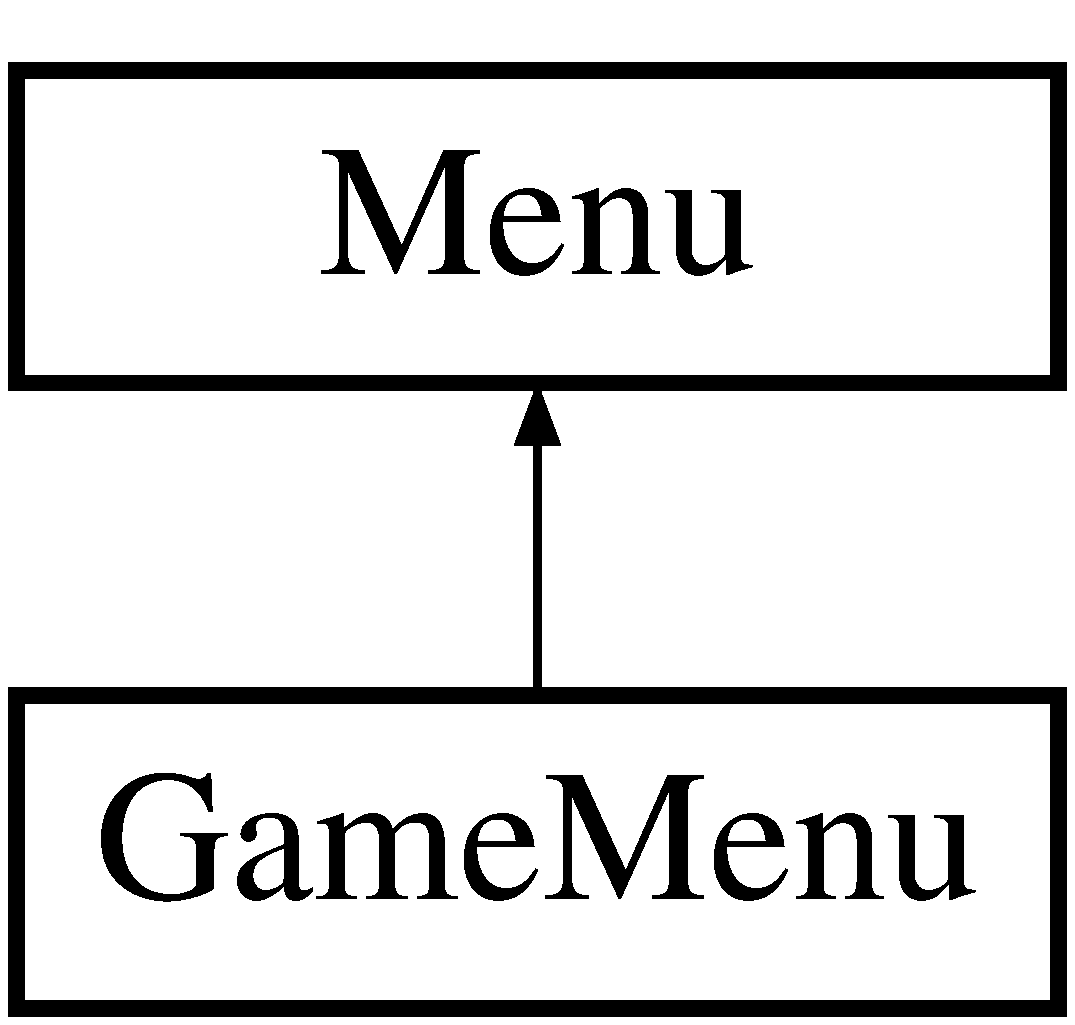
\includegraphics[height=2.000000cm]{class_game_menu}
\end{center}
\end{figure}
\subsection*{Public Member Functions}
\begin{DoxyCompactItemize}
\item 
\hyperlink{class_game_menu_ae31c50148abf655297a2a3eab53c15a3}{Game\+Menu} ()
\item 
\hyperlink{class_game_menu_ac3c079d7180f1127d86c7f44c34c4f5d}{Game\+Menu} (std\+::string my\+Texture\+Address, sf\+::\+Vector2u my\+Size, sf\+::\+Vector2i my\+Position)
\item 
\hyperlink{class_game_menu_a70ac0e31f882993f09eb1bdbdd352a56}{$\sim$\+Game\+Menu} ()
\item 
void \hyperlink{class_game_menu_af564d47068179979d48904e73455a542}{opent} ()
\item 
float \hyperlink{class_game_menu_a601a07a24fe40342bdc678ded8d4b6e4}{get\+Game\+Speed} ()
\item 
void \hyperlink{class_game_menu_afe832b00cc0ac1e35b702391d613de25}{set\+Game\+Speed} (float)
\item 
void \hyperlink{class_game_menu_a248194828f1a914fd1f09d263a0326d0}{pause\+Game} ()
\item 
void \hyperlink{class_game_menu_a88426fac8dc01247d626a12f38643616}{speed\+Game} ()
\item 
void \hyperlink{class_game_menu_a9f77fb9dcfdebc1ba96af75ee3083abc}{return\+Speed} ()
\item 
void \hyperlink{class_game_menu_a77617acfe92a25cf97d0da8197ff5e92}{restart\+Game} ()
\item 
void \hyperlink{class_game_menu_aabc9ea58600553c8562881d069c67d2c}{draw} (sf\+::\+Render\+Window \&w)
\item 
void \hyperlink{class_game_menu_a9dd958097e685b1904cdc1c8d2a9ffff}{resolve\+Event} (sf\+::\+Event event)
\end{DoxyCompactItemize}
\subsection*{Additional Inherited Members}


\subsection{Constructor \& Destructor Documentation}
\hypertarget{class_game_menu_ae31c50148abf655297a2a3eab53c15a3}{\index{Game\+Menu@{Game\+Menu}!Game\+Menu@{Game\+Menu}}
\index{Game\+Menu@{Game\+Menu}!Game\+Menu@{Game\+Menu}}
\subsubsection[{Game\+Menu}]{\setlength{\rightskip}{0pt plus 5cm}Game\+Menu\+::\+Game\+Menu (
\begin{DoxyParamCaption}
{}
\end{DoxyParamCaption}
)}}\label{class_game_menu_ae31c50148abf655297a2a3eab53c15a3}
\hypertarget{class_game_menu_ac3c079d7180f1127d86c7f44c34c4f5d}{\index{Game\+Menu@{Game\+Menu}!Game\+Menu@{Game\+Menu}}
\index{Game\+Menu@{Game\+Menu}!Game\+Menu@{Game\+Menu}}
\subsubsection[{Game\+Menu}]{\setlength{\rightskip}{0pt plus 5cm}Game\+Menu\+::\+Game\+Menu (
\begin{DoxyParamCaption}
\item[{std\+::string}]{my\+Texture\+Address, }
\item[{sf\+::\+Vector2u}]{my\+Size, }
\item[{sf\+::\+Vector2i}]{my\+Position}
\end{DoxyParamCaption}
)}}\label{class_game_menu_ac3c079d7180f1127d86c7f44c34c4f5d}
\hypertarget{class_game_menu_a70ac0e31f882993f09eb1bdbdd352a56}{\index{Game\+Menu@{Game\+Menu}!````~Game\+Menu@{$\sim$\+Game\+Menu}}
\index{````~Game\+Menu@{$\sim$\+Game\+Menu}!Game\+Menu@{Game\+Menu}}
\subsubsection[{$\sim$\+Game\+Menu}]{\setlength{\rightskip}{0pt plus 5cm}Game\+Menu\+::$\sim$\+Game\+Menu (
\begin{DoxyParamCaption}
{}
\end{DoxyParamCaption}
)}}\label{class_game_menu_a70ac0e31f882993f09eb1bdbdd352a56}


\subsection{Member Function Documentation}
\hypertarget{class_game_menu_aabc9ea58600553c8562881d069c67d2c}{\index{Game\+Menu@{Game\+Menu}!draw@{draw}}
\index{draw@{draw}!Game\+Menu@{Game\+Menu}}
\subsubsection[{draw}]{\setlength{\rightskip}{0pt plus 5cm}void Game\+Menu\+::draw (
\begin{DoxyParamCaption}
\item[{sf\+::\+Render\+Window \&}]{w}
\end{DoxyParamCaption}
)\hspace{0.3cm}{\ttfamily [virtual]}}}\label{class_game_menu_aabc9ea58600553c8562881d069c67d2c}


Reimplemented from \hyperlink{class_menu_a5c486201ec217b10588c145d043e4eb8}{Menu}.

\hypertarget{class_game_menu_a601a07a24fe40342bdc678ded8d4b6e4}{\index{Game\+Menu@{Game\+Menu}!get\+Game\+Speed@{get\+Game\+Speed}}
\index{get\+Game\+Speed@{get\+Game\+Speed}!Game\+Menu@{Game\+Menu}}
\subsubsection[{get\+Game\+Speed}]{\setlength{\rightskip}{0pt plus 5cm}float Game\+Menu\+::get\+Game\+Speed (
\begin{DoxyParamCaption}
{}
\end{DoxyParamCaption}
)}}\label{class_game_menu_a601a07a24fe40342bdc678ded8d4b6e4}
\hypertarget{class_game_menu_af564d47068179979d48904e73455a542}{\index{Game\+Menu@{Game\+Menu}!opent@{opent}}
\index{opent@{opent}!Game\+Menu@{Game\+Menu}}
\subsubsection[{opent}]{\setlength{\rightskip}{0pt plus 5cm}void Game\+Menu\+::opent (
\begin{DoxyParamCaption}
{}
\end{DoxyParamCaption}
)\hspace{0.3cm}{\ttfamily [inline]}}}\label{class_game_menu_af564d47068179979d48904e73455a542}
\hypertarget{class_game_menu_a248194828f1a914fd1f09d263a0326d0}{\index{Game\+Menu@{Game\+Menu}!pause\+Game@{pause\+Game}}
\index{pause\+Game@{pause\+Game}!Game\+Menu@{Game\+Menu}}
\subsubsection[{pause\+Game}]{\setlength{\rightskip}{0pt plus 5cm}void Game\+Menu\+::pause\+Game (
\begin{DoxyParamCaption}
{}
\end{DoxyParamCaption}
)}}\label{class_game_menu_a248194828f1a914fd1f09d263a0326d0}
\hypertarget{class_game_menu_a9dd958097e685b1904cdc1c8d2a9ffff}{\index{Game\+Menu@{Game\+Menu}!resolve\+Event@{resolve\+Event}}
\index{resolve\+Event@{resolve\+Event}!Game\+Menu@{Game\+Menu}}
\subsubsection[{resolve\+Event}]{\setlength{\rightskip}{0pt plus 5cm}void Game\+Menu\+::resolve\+Event (
\begin{DoxyParamCaption}
\item[{sf\+::\+Event}]{event}
\end{DoxyParamCaption}
)\hspace{0.3cm}{\ttfamily [virtual]}}}\label{class_game_menu_a9dd958097e685b1904cdc1c8d2a9ffff}


Implements \hyperlink{class_menu_a91ec4d6d898e740524b1fe3312d8f197}{Menu}.

\hypertarget{class_game_menu_a77617acfe92a25cf97d0da8197ff5e92}{\index{Game\+Menu@{Game\+Menu}!restart\+Game@{restart\+Game}}
\index{restart\+Game@{restart\+Game}!Game\+Menu@{Game\+Menu}}
\subsubsection[{restart\+Game}]{\setlength{\rightskip}{0pt plus 5cm}void Game\+Menu\+::restart\+Game (
\begin{DoxyParamCaption}
{}
\end{DoxyParamCaption}
)}}\label{class_game_menu_a77617acfe92a25cf97d0da8197ff5e92}
\hypertarget{class_game_menu_a9f77fb9dcfdebc1ba96af75ee3083abc}{\index{Game\+Menu@{Game\+Menu}!return\+Speed@{return\+Speed}}
\index{return\+Speed@{return\+Speed}!Game\+Menu@{Game\+Menu}}
\subsubsection[{return\+Speed}]{\setlength{\rightskip}{0pt plus 5cm}void Game\+Menu\+::return\+Speed (
\begin{DoxyParamCaption}
{}
\end{DoxyParamCaption}
)}}\label{class_game_menu_a9f77fb9dcfdebc1ba96af75ee3083abc}
\hypertarget{class_game_menu_afe832b00cc0ac1e35b702391d613de25}{\index{Game\+Menu@{Game\+Menu}!set\+Game\+Speed@{set\+Game\+Speed}}
\index{set\+Game\+Speed@{set\+Game\+Speed}!Game\+Menu@{Game\+Menu}}
\subsubsection[{set\+Game\+Speed}]{\setlength{\rightskip}{0pt plus 5cm}void Game\+Menu\+::set\+Game\+Speed (
\begin{DoxyParamCaption}
\item[{float}]{my\+Game\+Speed}
\end{DoxyParamCaption}
)}}\label{class_game_menu_afe832b00cc0ac1e35b702391d613de25}
\hypertarget{class_game_menu_a88426fac8dc01247d626a12f38643616}{\index{Game\+Menu@{Game\+Menu}!speed\+Game@{speed\+Game}}
\index{speed\+Game@{speed\+Game}!Game\+Menu@{Game\+Menu}}
\subsubsection[{speed\+Game}]{\setlength{\rightskip}{0pt plus 5cm}void Game\+Menu\+::speed\+Game (
\begin{DoxyParamCaption}
{}
\end{DoxyParamCaption}
)}}\label{class_game_menu_a88426fac8dc01247d626a12f38643616}


The documentation for this class was generated from the following files\+:\begin{DoxyCompactItemize}
\item 
D\+:/\+Tower\+Defense/\+Tower\+Defense/\hyperlink{_game_menu_8h}{Game\+Menu.\+h}\item 
D\+:/\+Tower\+Defense/\+Tower\+Defense/\hyperlink{_game_menu_8cpp}{Game\+Menu.\+cpp}\end{DoxyCompactItemize}

\hypertarget{class_game_over_menu}{\section{Game\+Over\+Menu Class Reference}
\label{class_game_over_menu}\index{Game\+Over\+Menu@{Game\+Over\+Menu}}
}


{\ttfamily \#include $<$Game\+Over\+Menu.\+h$>$}

Inheritance diagram for Game\+Over\+Menu\+:\begin{figure}[H]
\begin{center}
\leavevmode
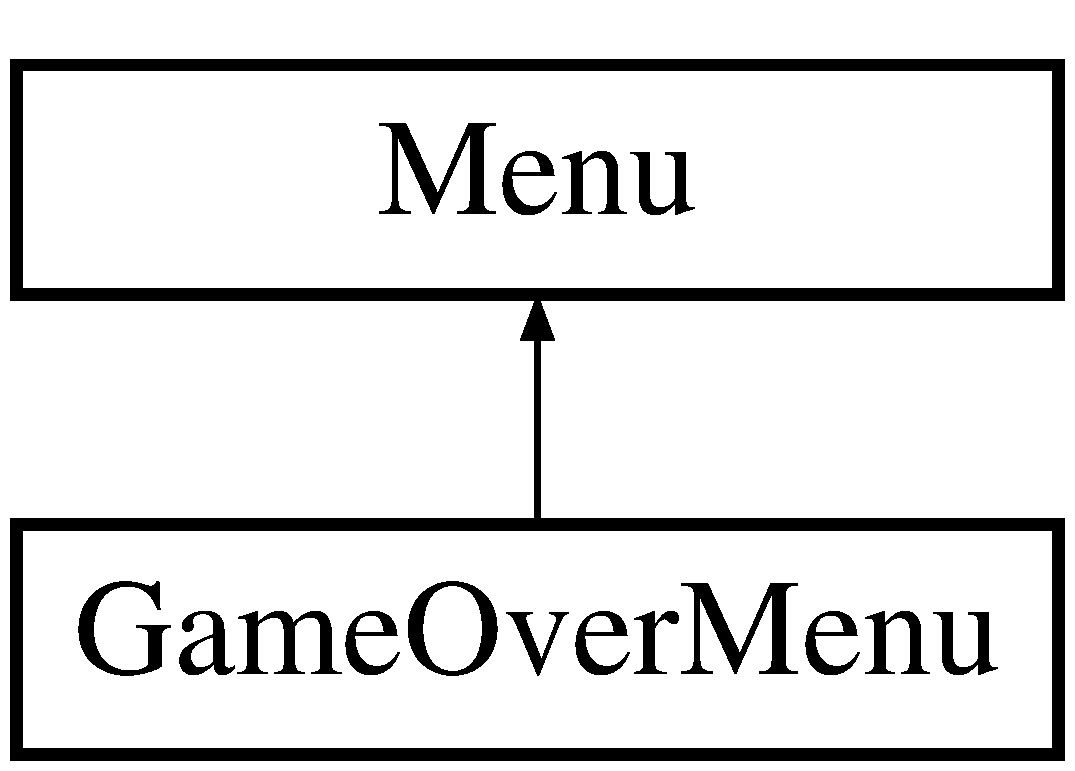
\includegraphics[height=2.000000cm]{class_game_over_menu}
\end{center}
\end{figure}
\subsection*{Public Member Functions}
\begin{DoxyCompactItemize}
\item 
\hyperlink{class_game_over_menu_a4dca1c9928485b1c726112992115bbf8}{Game\+Over\+Menu} ()
\item 
\hyperlink{class_game_over_menu_ab290478651ee389837bde740bbc6f3dc}{Game\+Over\+Menu} (std\+::string, sf\+::\+Vector2u, sf\+::\+Vector2i)
\item 
\hyperlink{class_game_over_menu_a4d1cc3861255f9d4f3f6da073259f0f1}{$\sim$\+Game\+Over\+Menu} ()
\item 
void \hyperlink{class_game_over_menu_a5e67d2adec64c94bd880b608c72c4453}{draw} (sf\+::\+Render\+Window \&)
\item 
void \hyperlink{class_game_over_menu_a2b73cda98b30f7c20c5607b6ca8a6915}{resolve\+Event} (sf\+::\+Event)
\item 
void \hyperlink{class_game_over_menu_a1c01e4275b763f83b14301353c873899}{re\+Start\+Game} ()
\item 
void \hyperlink{class_game_over_menu_abb28ebaf2def30a8fc15434639a483e4}{exit\+Game} ()
\end{DoxyCompactItemize}
\subsection*{Additional Inherited Members}


\subsection{Constructor \& Destructor Documentation}
\hypertarget{class_game_over_menu_a4dca1c9928485b1c726112992115bbf8}{\index{Game\+Over\+Menu@{Game\+Over\+Menu}!Game\+Over\+Menu@{Game\+Over\+Menu}}
\index{Game\+Over\+Menu@{Game\+Over\+Menu}!Game\+Over\+Menu@{Game\+Over\+Menu}}
\subsubsection[{Game\+Over\+Menu}]{\setlength{\rightskip}{0pt plus 5cm}Game\+Over\+Menu\+::\+Game\+Over\+Menu (
\begin{DoxyParamCaption}
{}
\end{DoxyParamCaption}
)}}\label{class_game_over_menu_a4dca1c9928485b1c726112992115bbf8}
\hypertarget{class_game_over_menu_ab290478651ee389837bde740bbc6f3dc}{\index{Game\+Over\+Menu@{Game\+Over\+Menu}!Game\+Over\+Menu@{Game\+Over\+Menu}}
\index{Game\+Over\+Menu@{Game\+Over\+Menu}!Game\+Over\+Menu@{Game\+Over\+Menu}}
\subsubsection[{Game\+Over\+Menu}]{\setlength{\rightskip}{0pt plus 5cm}Game\+Over\+Menu\+::\+Game\+Over\+Menu (
\begin{DoxyParamCaption}
\item[{std\+::string}]{my\+Texture\+Address, }
\item[{sf\+::\+Vector2u}]{my\+Size, }
\item[{sf\+::\+Vector2i}]{my\+Position}
\end{DoxyParamCaption}
)}}\label{class_game_over_menu_ab290478651ee389837bde740bbc6f3dc}
\hypertarget{class_game_over_menu_a4d1cc3861255f9d4f3f6da073259f0f1}{\index{Game\+Over\+Menu@{Game\+Over\+Menu}!````~Game\+Over\+Menu@{$\sim$\+Game\+Over\+Menu}}
\index{````~Game\+Over\+Menu@{$\sim$\+Game\+Over\+Menu}!Game\+Over\+Menu@{Game\+Over\+Menu}}
\subsubsection[{$\sim$\+Game\+Over\+Menu}]{\setlength{\rightskip}{0pt plus 5cm}Game\+Over\+Menu\+::$\sim$\+Game\+Over\+Menu (
\begin{DoxyParamCaption}
{}
\end{DoxyParamCaption}
)}}\label{class_game_over_menu_a4d1cc3861255f9d4f3f6da073259f0f1}


\subsection{Member Function Documentation}
\hypertarget{class_game_over_menu_a5e67d2adec64c94bd880b608c72c4453}{\index{Game\+Over\+Menu@{Game\+Over\+Menu}!draw@{draw}}
\index{draw@{draw}!Game\+Over\+Menu@{Game\+Over\+Menu}}
\subsubsection[{draw}]{\setlength{\rightskip}{0pt plus 5cm}void Game\+Over\+Menu\+::draw (
\begin{DoxyParamCaption}
\item[{sf\+::\+Render\+Window \&}]{w}
\end{DoxyParamCaption}
)\hspace{0.3cm}{\ttfamily [virtual]}}}\label{class_game_over_menu_a5e67d2adec64c94bd880b608c72c4453}


Reimplemented from \hyperlink{class_menu_a5c486201ec217b10588c145d043e4eb8}{Menu}.

\hypertarget{class_game_over_menu_abb28ebaf2def30a8fc15434639a483e4}{\index{Game\+Over\+Menu@{Game\+Over\+Menu}!exit\+Game@{exit\+Game}}
\index{exit\+Game@{exit\+Game}!Game\+Over\+Menu@{Game\+Over\+Menu}}
\subsubsection[{exit\+Game}]{\setlength{\rightskip}{0pt plus 5cm}void Game\+Over\+Menu\+::exit\+Game (
\begin{DoxyParamCaption}
{}
\end{DoxyParamCaption}
)}}\label{class_game_over_menu_abb28ebaf2def30a8fc15434639a483e4}
\hypertarget{class_game_over_menu_a2b73cda98b30f7c20c5607b6ca8a6915}{\index{Game\+Over\+Menu@{Game\+Over\+Menu}!resolve\+Event@{resolve\+Event}}
\index{resolve\+Event@{resolve\+Event}!Game\+Over\+Menu@{Game\+Over\+Menu}}
\subsubsection[{resolve\+Event}]{\setlength{\rightskip}{0pt plus 5cm}void Game\+Over\+Menu\+::resolve\+Event (
\begin{DoxyParamCaption}
\item[{sf\+::\+Event}]{event}
\end{DoxyParamCaption}
)\hspace{0.3cm}{\ttfamily [virtual]}}}\label{class_game_over_menu_a2b73cda98b30f7c20c5607b6ca8a6915}


Implements \hyperlink{class_menu_a91ec4d6d898e740524b1fe3312d8f197}{Menu}.

\hypertarget{class_game_over_menu_a1c01e4275b763f83b14301353c873899}{\index{Game\+Over\+Menu@{Game\+Over\+Menu}!re\+Start\+Game@{re\+Start\+Game}}
\index{re\+Start\+Game@{re\+Start\+Game}!Game\+Over\+Menu@{Game\+Over\+Menu}}
\subsubsection[{re\+Start\+Game}]{\setlength{\rightskip}{0pt plus 5cm}void Game\+Over\+Menu\+::re\+Start\+Game (
\begin{DoxyParamCaption}
{}
\end{DoxyParamCaption}
)}}\label{class_game_over_menu_a1c01e4275b763f83b14301353c873899}


The documentation for this class was generated from the following files\+:\begin{DoxyCompactItemize}
\item 
D\+:/\+Tower\+Defense/\+Tower\+Defense/\hyperlink{_game_over_menu_8h}{Game\+Over\+Menu.\+h}\item 
D\+:/\+Tower\+Defense/\+Tower\+Defense/\hyperlink{_game_over_menu_8cpp}{Game\+Over\+Menu.\+cpp}\end{DoxyCompactItemize}

\hypertarget{class_level_manager}{\section{Level\+Manager Class Reference}
\label{class_level_manager}\index{Level\+Manager@{Level\+Manager}}
}


{\ttfamily \#include $<$Level\+Manager.\+h$>$}

\subsection*{Public Member Functions}
\begin{DoxyCompactItemize}
\item 
void \hyperlink{class_level_manager_a08e53dd6adc768f11fe228237f69812c}{kill} ()
\item 
void \hyperlink{class_level_manager_aa5fe71c398e90bbe0692bee8482565ff}{game\+Loop} (sf\+::\+Render\+Window \&w)
\item 
void \hyperlink{class_level_manager_a6e65b26fe458b839abc10edd582fae92}{add\+Enemy} (shared\+\_\+ptr$<$ \hyperlink{class_enemy}{Enemy} $>$ e)
\item 
void \hyperlink{class_level_manager_ab39faffd3cdf1b0db93e9a16309e165b}{remove\+Enemy} (shared\+\_\+ptr$<$ \hyperlink{class_enemy}{Enemy} $>$ e)
\item 
void \hyperlink{class_level_manager_ab30f1cdbbea36dd751a8d913c3ab032c}{remove\+Enemy} (int)
\item 
void \hyperlink{class_level_manager_aefa59f244e5ea86cc3f9d70943abfd16}{add\+Tower} (shared\+\_\+ptr$<$ \hyperlink{class_tower}{Tower} $>$)
\item 
void \hyperlink{class_level_manager_aa4824d853f1f46990bb751e7fdb76968}{remove\+Tower} (shared\+\_\+ptr$<$ \hyperlink{class_tower}{Tower} $>$)
\item 
void \hyperlink{class_level_manager_abc16dc36bc6303695e3b80475864b52b}{remove\+Tower} (int)
\item 
vector$<$ shared\+\_\+ptr$<$ \hyperlink{class_enemy}{Enemy} $>$ $>$ \hyperlink{class_level_manager_adbec76ac05350f5ad5225947893a198f}{get\+Enemies} ()
\item 
vector$<$ shared\+\_\+ptr$<$ \hyperlink{class_tower}{Tower} $>$ $>$ \hyperlink{class_level_manager_a3e72274151623dbe0ca48fb4c6ab5671}{get\+Towers} ()
\item 
vector$<$ \hyperlink{class_wave}{Wave} $>$ \hyperlink{class_level_manager_a0d63a324a0cd404302d64270099884f0}{get\+Waves} ()
\item 
void \hyperlink{class_level_manager_ae82f34baef0c9bd5e4b9db6156b45f85}{set\+Player} (shared\+\_\+ptr$<$ \hyperlink{class_player}{Player} $>$ player)
\item 
shared\+\_\+ptr$<$ \hyperlink{class_player}{Player} $>$ \hyperlink{class_level_manager_acb860de9f9ccb23b4a799d857bec1cf9}{get\+Player} ()
\item 
bool \hyperlink{class_level_manager_abb8626a3a8aac40f066c203faac35b20}{if\+Win} ()
\item 
void \hyperlink{class_level_manager_a4435cdb4ae2d199c372d4047f0dc0c92}{set\+Field} (\hyperlink{class_field}{Field} \&field)
\item 
\hyperlink{class_field}{Field} \hyperlink{class_level_manager_aa0968f6bf0d80f7b50658aca7f487508}{get\+Field} ()
\item 
int \hyperlink{class_level_manager_a8794dccc6438fc2058a78d625f508841}{get\+Speed} ()
\item 
void \hyperlink{class_level_manager_ab7945c7629de9d3e77bf6328779aed35}{set\+Speed} (int)
\item 
void \hyperlink{class_level_manager_aa883e507745c8d405ef2cdd2b6351dfa}{next\+Wave} ()
\item 
void \hyperlink{class_level_manager_a4cb7dacced44be50765c930e5e73f217}{load\+Waves} ()
\item 
void \hyperlink{class_level_manager_a53c800a80f6f78702d6eaf3b43ca2d2b}{update\+Path} ()
\item 
void \hyperlink{class_level_manager_a488b4c395d164dc5b1975b69f45eb9ac}{game\+Over} ()
\item 
void \hyperlink{class_level_manager_a3fda56827462d66760c612c2a382fc05}{victory} ()
\item 
int \hyperlink{class_level_manager_a7d1ad576cc249a90c17fd06fa907976a}{stop\+Game} ()
\item 
void \hyperlink{class_level_manager_a128f679f42d155e38a657feac3c2cc78}{start\+Game} ()
\item 
void \hyperlink{class_level_manager_a23dcc64c396c58ac864c7d032b3618cf}{restart\+Game} ()
\item 
int \hyperlink{class_level_manager_a7e3e06f49d24c49be1a58124a2aa92eb}{get\+Current\+Wave\+Number} ()
\end{DoxyCompactItemize}
\subsection*{Static Public Member Functions}
\begin{DoxyCompactItemize}
\item 
static \hyperlink{class_level_manager}{Level\+Manager} $\ast$ \hyperlink{class_level_manager_a0c42183e70000a197ac63a631fc14c97}{get\+Level\+Manager} ()
\end{DoxyCompactItemize}


\subsection{Member Function Documentation}
\hypertarget{class_level_manager_a6e65b26fe458b839abc10edd582fae92}{\index{Level\+Manager@{Level\+Manager}!add\+Enemy@{add\+Enemy}}
\index{add\+Enemy@{add\+Enemy}!Level\+Manager@{Level\+Manager}}
\subsubsection[{add\+Enemy}]{\setlength{\rightskip}{0pt plus 5cm}void Level\+Manager\+::add\+Enemy (
\begin{DoxyParamCaption}
\item[{shared\+\_\+ptr$<$ {\bf Enemy} $>$}]{e}
\end{DoxyParamCaption}
)}}\label{class_level_manager_a6e65b26fe458b839abc10edd582fae92}
\hypertarget{class_level_manager_aefa59f244e5ea86cc3f9d70943abfd16}{\index{Level\+Manager@{Level\+Manager}!add\+Tower@{add\+Tower}}
\index{add\+Tower@{add\+Tower}!Level\+Manager@{Level\+Manager}}
\subsubsection[{add\+Tower}]{\setlength{\rightskip}{0pt plus 5cm}void Level\+Manager\+::add\+Tower (
\begin{DoxyParamCaption}
\item[{shared\+\_\+ptr$<$ {\bf Tower} $>$}]{t}
\end{DoxyParamCaption}
)}}\label{class_level_manager_aefa59f244e5ea86cc3f9d70943abfd16}
\hypertarget{class_level_manager_aa5fe71c398e90bbe0692bee8482565ff}{\index{Level\+Manager@{Level\+Manager}!game\+Loop@{game\+Loop}}
\index{game\+Loop@{game\+Loop}!Level\+Manager@{Level\+Manager}}
\subsubsection[{game\+Loop}]{\setlength{\rightskip}{0pt plus 5cm}void Level\+Manager\+::game\+Loop (
\begin{DoxyParamCaption}
\item[{sf\+::\+Render\+Window \&}]{w}
\end{DoxyParamCaption}
)}}\label{class_level_manager_aa5fe71c398e90bbe0692bee8482565ff}
\hypertarget{class_level_manager_a488b4c395d164dc5b1975b69f45eb9ac}{\index{Level\+Manager@{Level\+Manager}!game\+Over@{game\+Over}}
\index{game\+Over@{game\+Over}!Level\+Manager@{Level\+Manager}}
\subsubsection[{game\+Over}]{\setlength{\rightskip}{0pt plus 5cm}void Level\+Manager\+::game\+Over (
\begin{DoxyParamCaption}
{}
\end{DoxyParamCaption}
)}}\label{class_level_manager_a488b4c395d164dc5b1975b69f45eb9ac}
\hypertarget{class_level_manager_a7e3e06f49d24c49be1a58124a2aa92eb}{\index{Level\+Manager@{Level\+Manager}!get\+Current\+Wave\+Number@{get\+Current\+Wave\+Number}}
\index{get\+Current\+Wave\+Number@{get\+Current\+Wave\+Number}!Level\+Manager@{Level\+Manager}}
\subsubsection[{get\+Current\+Wave\+Number}]{\setlength{\rightskip}{0pt plus 5cm}int Level\+Manager\+::get\+Current\+Wave\+Number (
\begin{DoxyParamCaption}
{}
\end{DoxyParamCaption}
)}}\label{class_level_manager_a7e3e06f49d24c49be1a58124a2aa92eb}
\hypertarget{class_level_manager_adbec76ac05350f5ad5225947893a198f}{\index{Level\+Manager@{Level\+Manager}!get\+Enemies@{get\+Enemies}}
\index{get\+Enemies@{get\+Enemies}!Level\+Manager@{Level\+Manager}}
\subsubsection[{get\+Enemies}]{\setlength{\rightskip}{0pt plus 5cm}vector$<$ shared\+\_\+ptr$<$ {\bf Enemy} $>$ $>$ Level\+Manager\+::get\+Enemies (
\begin{DoxyParamCaption}
{}
\end{DoxyParamCaption}
)}}\label{class_level_manager_adbec76ac05350f5ad5225947893a198f}
\hypertarget{class_level_manager_aa0968f6bf0d80f7b50658aca7f487508}{\index{Level\+Manager@{Level\+Manager}!get\+Field@{get\+Field}}
\index{get\+Field@{get\+Field}!Level\+Manager@{Level\+Manager}}
\subsubsection[{get\+Field}]{\setlength{\rightskip}{0pt plus 5cm}{\bf Field} Level\+Manager\+::get\+Field (
\begin{DoxyParamCaption}
{}
\end{DoxyParamCaption}
)}}\label{class_level_manager_aa0968f6bf0d80f7b50658aca7f487508}
\hypertarget{class_level_manager_a0c42183e70000a197ac63a631fc14c97}{\index{Level\+Manager@{Level\+Manager}!get\+Level\+Manager@{get\+Level\+Manager}}
\index{get\+Level\+Manager@{get\+Level\+Manager}!Level\+Manager@{Level\+Manager}}
\subsubsection[{get\+Level\+Manager}]{\setlength{\rightskip}{0pt plus 5cm}{\bf Level\+Manager} $\ast$ Level\+Manager\+::get\+Level\+Manager (
\begin{DoxyParamCaption}
{}
\end{DoxyParamCaption}
)\hspace{0.3cm}{\ttfamily [static]}}}\label{class_level_manager_a0c42183e70000a197ac63a631fc14c97}
\hypertarget{class_level_manager_acb860de9f9ccb23b4a799d857bec1cf9}{\index{Level\+Manager@{Level\+Manager}!get\+Player@{get\+Player}}
\index{get\+Player@{get\+Player}!Level\+Manager@{Level\+Manager}}
\subsubsection[{get\+Player}]{\setlength{\rightskip}{0pt plus 5cm}shared\+\_\+ptr$<$ {\bf Player} $>$ Level\+Manager\+::get\+Player (
\begin{DoxyParamCaption}
{}
\end{DoxyParamCaption}
)}}\label{class_level_manager_acb860de9f9ccb23b4a799d857bec1cf9}
\hypertarget{class_level_manager_a8794dccc6438fc2058a78d625f508841}{\index{Level\+Manager@{Level\+Manager}!get\+Speed@{get\+Speed}}
\index{get\+Speed@{get\+Speed}!Level\+Manager@{Level\+Manager}}
\subsubsection[{get\+Speed}]{\setlength{\rightskip}{0pt plus 5cm}int Level\+Manager\+::get\+Speed (
\begin{DoxyParamCaption}
{}
\end{DoxyParamCaption}
)}}\label{class_level_manager_a8794dccc6438fc2058a78d625f508841}
\hypertarget{class_level_manager_a3e72274151623dbe0ca48fb4c6ab5671}{\index{Level\+Manager@{Level\+Manager}!get\+Towers@{get\+Towers}}
\index{get\+Towers@{get\+Towers}!Level\+Manager@{Level\+Manager}}
\subsubsection[{get\+Towers}]{\setlength{\rightskip}{0pt plus 5cm}vector$<$ shared\+\_\+ptr$<$ {\bf Tower} $>$ $>$ Level\+Manager\+::get\+Towers (
\begin{DoxyParamCaption}
{}
\end{DoxyParamCaption}
)}}\label{class_level_manager_a3e72274151623dbe0ca48fb4c6ab5671}
\hypertarget{class_level_manager_a0d63a324a0cd404302d64270099884f0}{\index{Level\+Manager@{Level\+Manager}!get\+Waves@{get\+Waves}}
\index{get\+Waves@{get\+Waves}!Level\+Manager@{Level\+Manager}}
\subsubsection[{get\+Waves}]{\setlength{\rightskip}{0pt plus 5cm}vector$<${\bf Wave}$>$ Level\+Manager\+::get\+Waves (
\begin{DoxyParamCaption}
{}
\end{DoxyParamCaption}
)}}\label{class_level_manager_a0d63a324a0cd404302d64270099884f0}
\hypertarget{class_level_manager_abb8626a3a8aac40f066c203faac35b20}{\index{Level\+Manager@{Level\+Manager}!if\+Win@{if\+Win}}
\index{if\+Win@{if\+Win}!Level\+Manager@{Level\+Manager}}
\subsubsection[{if\+Win}]{\setlength{\rightskip}{0pt plus 5cm}bool Level\+Manager\+::if\+Win (
\begin{DoxyParamCaption}
{}
\end{DoxyParamCaption}
)}}\label{class_level_manager_abb8626a3a8aac40f066c203faac35b20}
\hypertarget{class_level_manager_a08e53dd6adc768f11fe228237f69812c}{\index{Level\+Manager@{Level\+Manager}!kill@{kill}}
\index{kill@{kill}!Level\+Manager@{Level\+Manager}}
\subsubsection[{kill}]{\setlength{\rightskip}{0pt plus 5cm}void Level\+Manager\+::kill (
\begin{DoxyParamCaption}
{}
\end{DoxyParamCaption}
)}}\label{class_level_manager_a08e53dd6adc768f11fe228237f69812c}
\hypertarget{class_level_manager_a4cb7dacced44be50765c930e5e73f217}{\index{Level\+Manager@{Level\+Manager}!load\+Waves@{load\+Waves}}
\index{load\+Waves@{load\+Waves}!Level\+Manager@{Level\+Manager}}
\subsubsection[{load\+Waves}]{\setlength{\rightskip}{0pt plus 5cm}void Level\+Manager\+::load\+Waves (
\begin{DoxyParamCaption}
{}
\end{DoxyParamCaption}
)}}\label{class_level_manager_a4cb7dacced44be50765c930e5e73f217}
\hypertarget{class_level_manager_aa883e507745c8d405ef2cdd2b6351dfa}{\index{Level\+Manager@{Level\+Manager}!next\+Wave@{next\+Wave}}
\index{next\+Wave@{next\+Wave}!Level\+Manager@{Level\+Manager}}
\subsubsection[{next\+Wave}]{\setlength{\rightskip}{0pt plus 5cm}void Level\+Manager\+::next\+Wave (
\begin{DoxyParamCaption}
{}
\end{DoxyParamCaption}
)}}\label{class_level_manager_aa883e507745c8d405ef2cdd2b6351dfa}
\hypertarget{class_level_manager_ab39faffd3cdf1b0db93e9a16309e165b}{\index{Level\+Manager@{Level\+Manager}!remove\+Enemy@{remove\+Enemy}}
\index{remove\+Enemy@{remove\+Enemy}!Level\+Manager@{Level\+Manager}}
\subsubsection[{remove\+Enemy}]{\setlength{\rightskip}{0pt plus 5cm}void Level\+Manager\+::remove\+Enemy (
\begin{DoxyParamCaption}
\item[{shared\+\_\+ptr$<$ {\bf Enemy} $>$}]{e}
\end{DoxyParamCaption}
)}}\label{class_level_manager_ab39faffd3cdf1b0db93e9a16309e165b}
\hypertarget{class_level_manager_ab30f1cdbbea36dd751a8d913c3ab032c}{\index{Level\+Manager@{Level\+Manager}!remove\+Enemy@{remove\+Enemy}}
\index{remove\+Enemy@{remove\+Enemy}!Level\+Manager@{Level\+Manager}}
\subsubsection[{remove\+Enemy}]{\setlength{\rightskip}{0pt plus 5cm}void Level\+Manager\+::remove\+Enemy (
\begin{DoxyParamCaption}
\item[{int}]{index}
\end{DoxyParamCaption}
)}}\label{class_level_manager_ab30f1cdbbea36dd751a8d913c3ab032c}
\hypertarget{class_level_manager_aa4824d853f1f46990bb751e7fdb76968}{\index{Level\+Manager@{Level\+Manager}!remove\+Tower@{remove\+Tower}}
\index{remove\+Tower@{remove\+Tower}!Level\+Manager@{Level\+Manager}}
\subsubsection[{remove\+Tower}]{\setlength{\rightskip}{0pt plus 5cm}void Level\+Manager\+::remove\+Tower (
\begin{DoxyParamCaption}
\item[{shared\+\_\+ptr$<$ {\bf Tower} $>$}]{t}
\end{DoxyParamCaption}
)}}\label{class_level_manager_aa4824d853f1f46990bb751e7fdb76968}
\hypertarget{class_level_manager_abc16dc36bc6303695e3b80475864b52b}{\index{Level\+Manager@{Level\+Manager}!remove\+Tower@{remove\+Tower}}
\index{remove\+Tower@{remove\+Tower}!Level\+Manager@{Level\+Manager}}
\subsubsection[{remove\+Tower}]{\setlength{\rightskip}{0pt plus 5cm}void Level\+Manager\+::remove\+Tower (
\begin{DoxyParamCaption}
\item[{int}]{index}
\end{DoxyParamCaption}
)}}\label{class_level_manager_abc16dc36bc6303695e3b80475864b52b}
\hypertarget{class_level_manager_a23dcc64c396c58ac864c7d032b3618cf}{\index{Level\+Manager@{Level\+Manager}!restart\+Game@{restart\+Game}}
\index{restart\+Game@{restart\+Game}!Level\+Manager@{Level\+Manager}}
\subsubsection[{restart\+Game}]{\setlength{\rightskip}{0pt plus 5cm}void Level\+Manager\+::restart\+Game (
\begin{DoxyParamCaption}
{}
\end{DoxyParamCaption}
)}}\label{class_level_manager_a23dcc64c396c58ac864c7d032b3618cf}
\hypertarget{class_level_manager_a4435cdb4ae2d199c372d4047f0dc0c92}{\index{Level\+Manager@{Level\+Manager}!set\+Field@{set\+Field}}
\index{set\+Field@{set\+Field}!Level\+Manager@{Level\+Manager}}
\subsubsection[{set\+Field}]{\setlength{\rightskip}{0pt plus 5cm}void Level\+Manager\+::set\+Field (
\begin{DoxyParamCaption}
\item[{{\bf Field} \&}]{field}
\end{DoxyParamCaption}
)}}\label{class_level_manager_a4435cdb4ae2d199c372d4047f0dc0c92}
\hypertarget{class_level_manager_ae82f34baef0c9bd5e4b9db6156b45f85}{\index{Level\+Manager@{Level\+Manager}!set\+Player@{set\+Player}}
\index{set\+Player@{set\+Player}!Level\+Manager@{Level\+Manager}}
\subsubsection[{set\+Player}]{\setlength{\rightskip}{0pt plus 5cm}void Level\+Manager\+::set\+Player (
\begin{DoxyParamCaption}
\item[{shared\+\_\+ptr$<$ {\bf Player} $>$}]{player}
\end{DoxyParamCaption}
)}}\label{class_level_manager_ae82f34baef0c9bd5e4b9db6156b45f85}
\hypertarget{class_level_manager_ab7945c7629de9d3e77bf6328779aed35}{\index{Level\+Manager@{Level\+Manager}!set\+Speed@{set\+Speed}}
\index{set\+Speed@{set\+Speed}!Level\+Manager@{Level\+Manager}}
\subsubsection[{set\+Speed}]{\setlength{\rightskip}{0pt plus 5cm}void Level\+Manager\+::set\+Speed (
\begin{DoxyParamCaption}
\item[{int}]{speed}
\end{DoxyParamCaption}
)}}\label{class_level_manager_ab7945c7629de9d3e77bf6328779aed35}
\hypertarget{class_level_manager_a128f679f42d155e38a657feac3c2cc78}{\index{Level\+Manager@{Level\+Manager}!start\+Game@{start\+Game}}
\index{start\+Game@{start\+Game}!Level\+Manager@{Level\+Manager}}
\subsubsection[{start\+Game}]{\setlength{\rightskip}{0pt plus 5cm}void Level\+Manager\+::start\+Game (
\begin{DoxyParamCaption}
{}
\end{DoxyParamCaption}
)}}\label{class_level_manager_a128f679f42d155e38a657feac3c2cc78}
\hypertarget{class_level_manager_a7d1ad576cc249a90c17fd06fa907976a}{\index{Level\+Manager@{Level\+Manager}!stop\+Game@{stop\+Game}}
\index{stop\+Game@{stop\+Game}!Level\+Manager@{Level\+Manager}}
\subsubsection[{stop\+Game}]{\setlength{\rightskip}{0pt plus 5cm}int Level\+Manager\+::stop\+Game (
\begin{DoxyParamCaption}
{}
\end{DoxyParamCaption}
)}}\label{class_level_manager_a7d1ad576cc249a90c17fd06fa907976a}
\hypertarget{class_level_manager_a53c800a80f6f78702d6eaf3b43ca2d2b}{\index{Level\+Manager@{Level\+Manager}!update\+Path@{update\+Path}}
\index{update\+Path@{update\+Path}!Level\+Manager@{Level\+Manager}}
\subsubsection[{update\+Path}]{\setlength{\rightskip}{0pt plus 5cm}void Level\+Manager\+::update\+Path (
\begin{DoxyParamCaption}
{}
\end{DoxyParamCaption}
)}}\label{class_level_manager_a53c800a80f6f78702d6eaf3b43ca2d2b}
\hypertarget{class_level_manager_a3fda56827462d66760c612c2a382fc05}{\index{Level\+Manager@{Level\+Manager}!victory@{victory}}
\index{victory@{victory}!Level\+Manager@{Level\+Manager}}
\subsubsection[{victory}]{\setlength{\rightskip}{0pt plus 5cm}void Level\+Manager\+::victory (
\begin{DoxyParamCaption}
{}
\end{DoxyParamCaption}
)}}\label{class_level_manager_a3fda56827462d66760c612c2a382fc05}


The documentation for this class was generated from the following files\+:\begin{DoxyCompactItemize}
\item 
D\+:/\+Tower\+Defense/\+Tower\+Defense/\hyperlink{_level_manager_8h}{Level\+Manager.\+h}\item 
D\+:/\+Tower\+Defense/\+Tower\+Defense/\hyperlink{_level_manager_8cpp}{Level\+Manager.\+cpp}\end{DoxyCompactItemize}

\hypertarget{class_menu}{\section{Menu Class Reference}
\label{class_menu}\index{Menu@{Menu}}
}


{\ttfamily \#include $<$Menu.\+h$>$}

Inheritance diagram for Menu\+:\begin{figure}[H]
\begin{center}
\leavevmode
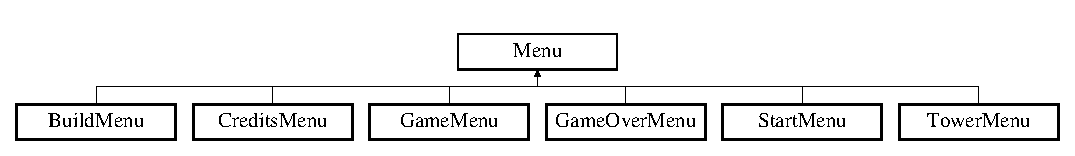
\includegraphics[height=1.651917cm]{class_menu}
\end{center}
\end{figure}
\subsection*{Public Member Functions}
\begin{DoxyCompactItemize}
\item 
\hyperlink{class_menu_ad466dd83355124a6ed958430450bfe94}{Menu} ()
\item 
\hyperlink{class_menu_af64b0c25ff426ce6b7819b1f24f17bd5}{Menu} (std\+::string my\+Texture\+Adress, sf\+::\+Vector2u my\+Size, sf\+::\+Vector2i my\+Position)
\item 
virtual \hyperlink{class_menu_a831387f51358cfb88cd018e1777bc980}{$\sim$\+Menu} ()
\item 
void \hyperlink{class_menu_a73160bee6f7a67c04ffe63b58fc19c7c}{set\+Size} (sf\+::\+Vector2u)
\item 
void \hyperlink{class_menu_a41687c51ee454954ce7ec116cc1f7459}{set\+Position} (sf\+::\+Vector2i)
\item 
void \hyperlink{class_menu_aade766e02b73948ebafb712ca9e53e12}{set\+Address} (std\+::string)
\item 
void \hyperlink{class_menu_a7d77cca2bf67824ebfb17b304950f2fc}{set\+Texture} (sf\+::\+Texture)
\item 
void \hyperlink{class_menu_a87144c354eae67283f29676a1d5207b6}{set\+Texture} (std\+::string)
\item 
void \hyperlink{class_menu_ae4f85d7309f7516a6147a5e8a85d1f7a}{set\+Sprite} (sf\+::\+Sprite)
\item 
void \hyperlink{class_menu_a98f348210794d6dbb3a5c5287f330e89}{set\+Sprite} (sf\+::\+Texture)
\item 
void \hyperlink{class_menu_afc4c1ec46b7e91299e1a0bbad98ea65e}{set\+Sprite} (std\+::string)
\item 
sf\+::\+Vector2u \hyperlink{class_menu_a570493d92f586ea813ecf3c9ea064bb9}{get\+Size} ()
\item 
sf\+::\+Vector2i \hyperlink{class_menu_ada5303b1b8997b3d117b8a553764d10f}{get\+Position} ()
\item 
sf\+::\+Sprite \hyperlink{class_menu_a2df8bb3db21a96e665e12bcaa0b3d5ef}{get\+Sprite} ()
\item 
sf\+::\+Texture \hyperlink{class_menu_a02124c4cb527346ac42b5c48235bea7f}{get\+Texture} ()
\item 
std\+::string \hyperlink{class_menu_a8eef8d68a55d02a9c12d6f1a2d832edc}{get\+Address} ()
\item 
virtual void \hyperlink{class_menu_a5c486201ec217b10588c145d043e4eb8}{draw} (sf\+::\+Render\+Window \&)
\item 
virtual void \hyperlink{class_menu_a4bc958c66bb39a91446b5c12ac6469c6}{close} ()
\item 
void \hyperlink{class_menu_a21202f42edbb5f1014ebe9f264613991}{opent} ()
\item 
virtual void \hyperlink{class_menu_a91ec4d6d898e740524b1fe3312d8f197}{resolve\+Event} (sf\+::\+Event)=0
\end{DoxyCompactItemize}
\subsection*{Protected Attributes}
\begin{DoxyCompactItemize}
\item 
sf\+::\+Sprite \hyperlink{class_menu_aa31afe4a4979a2c9ba427640af6e0909}{sprite}
\item 
sf\+::\+Texture \hyperlink{class_menu_a9be54103b9d80fc96cdc15d29da244b8}{texture}
\item 
std\+::string \hyperlink{class_menu_ae5ee6080fe5aad3dbee4935320e589b6}{texture\+Address}
\item 
sf\+::\+Vector2u \hyperlink{class_menu_ae43ea4415376f28f0d1c9b069614fde3}{size}
\item 
sf\+::\+Vector2i \hyperlink{class_menu_a5e6b181edbe72a18efff2eaa66cb97c4}{position}
\end{DoxyCompactItemize}


\subsection{Constructor \& Destructor Documentation}
\hypertarget{class_menu_ad466dd83355124a6ed958430450bfe94}{\index{Menu@{Menu}!Menu@{Menu}}
\index{Menu@{Menu}!Menu@{Menu}}
\subsubsection[{Menu}]{\setlength{\rightskip}{0pt plus 5cm}Menu\+::\+Menu (
\begin{DoxyParamCaption}
{}
\end{DoxyParamCaption}
)}}\label{class_menu_ad466dd83355124a6ed958430450bfe94}
\hypertarget{class_menu_af64b0c25ff426ce6b7819b1f24f17bd5}{\index{Menu@{Menu}!Menu@{Menu}}
\index{Menu@{Menu}!Menu@{Menu}}
\subsubsection[{Menu}]{\setlength{\rightskip}{0pt plus 5cm}Menu\+::\+Menu (
\begin{DoxyParamCaption}
\item[{std\+::string}]{my\+Texture\+Adress, }
\item[{sf\+::\+Vector2u}]{my\+Size, }
\item[{sf\+::\+Vector2i}]{my\+Position}
\end{DoxyParamCaption}
)}}\label{class_menu_af64b0c25ff426ce6b7819b1f24f17bd5}
\hypertarget{class_menu_a831387f51358cfb88cd018e1777bc980}{\index{Menu@{Menu}!````~Menu@{$\sim$\+Menu}}
\index{````~Menu@{$\sim$\+Menu}!Menu@{Menu}}
\subsubsection[{$\sim$\+Menu}]{\setlength{\rightskip}{0pt plus 5cm}Menu\+::$\sim$\+Menu (
\begin{DoxyParamCaption}
{}
\end{DoxyParamCaption}
)\hspace{0.3cm}{\ttfamily [virtual]}}}\label{class_menu_a831387f51358cfb88cd018e1777bc980}


\subsection{Member Function Documentation}
\hypertarget{class_menu_a4bc958c66bb39a91446b5c12ac6469c6}{\index{Menu@{Menu}!close@{close}}
\index{close@{close}!Menu@{Menu}}
\subsubsection[{close}]{\setlength{\rightskip}{0pt plus 5cm}void Menu\+::close (
\begin{DoxyParamCaption}
{}
\end{DoxyParamCaption}
)\hspace{0.3cm}{\ttfamily [virtual]}}}\label{class_menu_a4bc958c66bb39a91446b5c12ac6469c6}


Reimplemented in \hyperlink{class_tower_menu_afc1c7447eacd85abfa1f36ccdf3cbd7d}{Tower\+Menu}, and \hyperlink{class_build_menu_a58efd17837e0cd60a9bd1852cf6eaadd}{Build\+Menu}.

\hypertarget{class_menu_a5c486201ec217b10588c145d043e4eb8}{\index{Menu@{Menu}!draw@{draw}}
\index{draw@{draw}!Menu@{Menu}}
\subsubsection[{draw}]{\setlength{\rightskip}{0pt plus 5cm}void Menu\+::draw (
\begin{DoxyParamCaption}
\item[{sf\+::\+Render\+Window \&}]{w}
\end{DoxyParamCaption}
)\hspace{0.3cm}{\ttfamily [virtual]}}}\label{class_menu_a5c486201ec217b10588c145d043e4eb8}


Reimplemented in \hyperlink{class_tower_menu_a0ecd4cdad69ed36c06781035d77569bc}{Tower\+Menu}, \hyperlink{class_game_menu_aabc9ea58600553c8562881d069c67d2c}{Game\+Menu}, \hyperlink{class_build_menu_acbedc91d2b9c5ecf3d429612b95543a5}{Build\+Menu}, \hyperlink{class_start_menu_a34e56fc211d852a717bef5fc4136d13e}{Start\+Menu}, \hyperlink{class_credits_menu_a64fe7f7471ab92c69cbc95cb4ad9dfc8}{Credits\+Menu}, and \hyperlink{class_game_over_menu_a5e67d2adec64c94bd880b608c72c4453}{Game\+Over\+Menu}.

\hypertarget{class_menu_a8eef8d68a55d02a9c12d6f1a2d832edc}{\index{Menu@{Menu}!get\+Address@{get\+Address}}
\index{get\+Address@{get\+Address}!Menu@{Menu}}
\subsubsection[{get\+Address}]{\setlength{\rightskip}{0pt plus 5cm}std\+::string Menu\+::get\+Address (
\begin{DoxyParamCaption}
{}
\end{DoxyParamCaption}
)}}\label{class_menu_a8eef8d68a55d02a9c12d6f1a2d832edc}
\hypertarget{class_menu_ada5303b1b8997b3d117b8a553764d10f}{\index{Menu@{Menu}!get\+Position@{get\+Position}}
\index{get\+Position@{get\+Position}!Menu@{Menu}}
\subsubsection[{get\+Position}]{\setlength{\rightskip}{0pt plus 5cm}sf\+::\+Vector2i Menu\+::get\+Position (
\begin{DoxyParamCaption}
{}
\end{DoxyParamCaption}
)}}\label{class_menu_ada5303b1b8997b3d117b8a553764d10f}
\hypertarget{class_menu_a570493d92f586ea813ecf3c9ea064bb9}{\index{Menu@{Menu}!get\+Size@{get\+Size}}
\index{get\+Size@{get\+Size}!Menu@{Menu}}
\subsubsection[{get\+Size}]{\setlength{\rightskip}{0pt plus 5cm}sf\+::\+Vector2u Menu\+::get\+Size (
\begin{DoxyParamCaption}
{}
\end{DoxyParamCaption}
)}}\label{class_menu_a570493d92f586ea813ecf3c9ea064bb9}
\hypertarget{class_menu_a2df8bb3db21a96e665e12bcaa0b3d5ef}{\index{Menu@{Menu}!get\+Sprite@{get\+Sprite}}
\index{get\+Sprite@{get\+Sprite}!Menu@{Menu}}
\subsubsection[{get\+Sprite}]{\setlength{\rightskip}{0pt plus 5cm}sf\+::\+Sprite Menu\+::get\+Sprite (
\begin{DoxyParamCaption}
{}
\end{DoxyParamCaption}
)}}\label{class_menu_a2df8bb3db21a96e665e12bcaa0b3d5ef}
\hypertarget{class_menu_a02124c4cb527346ac42b5c48235bea7f}{\index{Menu@{Menu}!get\+Texture@{get\+Texture}}
\index{get\+Texture@{get\+Texture}!Menu@{Menu}}
\subsubsection[{get\+Texture}]{\setlength{\rightskip}{0pt plus 5cm}sf\+::\+Texture Menu\+::get\+Texture (
\begin{DoxyParamCaption}
{}
\end{DoxyParamCaption}
)}}\label{class_menu_a02124c4cb527346ac42b5c48235bea7f}
\hypertarget{class_menu_a21202f42edbb5f1014ebe9f264613991}{\index{Menu@{Menu}!opent@{opent}}
\index{opent@{opent}!Menu@{Menu}}
\subsubsection[{opent}]{\setlength{\rightskip}{0pt plus 5cm}void Menu\+::opent (
\begin{DoxyParamCaption}
{}
\end{DoxyParamCaption}
)}}\label{class_menu_a21202f42edbb5f1014ebe9f264613991}
\hypertarget{class_menu_a91ec4d6d898e740524b1fe3312d8f197}{\index{Menu@{Menu}!resolve\+Event@{resolve\+Event}}
\index{resolve\+Event@{resolve\+Event}!Menu@{Menu}}
\subsubsection[{resolve\+Event}]{\setlength{\rightskip}{0pt plus 5cm}void Menu\+::resolve\+Event (
\begin{DoxyParamCaption}
\item[{sf\+::\+Event}]{event}
\end{DoxyParamCaption}
)\hspace{0.3cm}{\ttfamily [pure virtual]}}}\label{class_menu_a91ec4d6d898e740524b1fe3312d8f197}


Implemented in \hyperlink{class_tower_menu_aacd3732231059c039a663f98fd6ec349}{Tower\+Menu}, \hyperlink{class_game_menu_a9dd958097e685b1904cdc1c8d2a9ffff}{Game\+Menu}, \hyperlink{class_build_menu_a2d044954ea1713a15048630e104c7d2a}{Build\+Menu}, \hyperlink{class_start_menu_a4f6701a9d7a4e08a5212c675ef1c66b2}{Start\+Menu}, \hyperlink{class_credits_menu_a6fa8421ffafa70e6d6e3af1f61b220c7}{Credits\+Menu}, and \hyperlink{class_game_over_menu_a2b73cda98b30f7c20c5607b6ca8a6915}{Game\+Over\+Menu}.

\hypertarget{class_menu_aade766e02b73948ebafb712ca9e53e12}{\index{Menu@{Menu}!set\+Address@{set\+Address}}
\index{set\+Address@{set\+Address}!Menu@{Menu}}
\subsubsection[{set\+Address}]{\setlength{\rightskip}{0pt plus 5cm}void Menu\+::set\+Address (
\begin{DoxyParamCaption}
\item[{std\+::string}]{}
\end{DoxyParamCaption}
)}}\label{class_menu_aade766e02b73948ebafb712ca9e53e12}
\hypertarget{class_menu_a41687c51ee454954ce7ec116cc1f7459}{\index{Menu@{Menu}!set\+Position@{set\+Position}}
\index{set\+Position@{set\+Position}!Menu@{Menu}}
\subsubsection[{set\+Position}]{\setlength{\rightskip}{0pt plus 5cm}void Menu\+::set\+Position (
\begin{DoxyParamCaption}
\item[{sf\+::\+Vector2i}]{my\+Position}
\end{DoxyParamCaption}
)}}\label{class_menu_a41687c51ee454954ce7ec116cc1f7459}
\hypertarget{class_menu_a73160bee6f7a67c04ffe63b58fc19c7c}{\index{Menu@{Menu}!set\+Size@{set\+Size}}
\index{set\+Size@{set\+Size}!Menu@{Menu}}
\subsubsection[{set\+Size}]{\setlength{\rightskip}{0pt plus 5cm}void Menu\+::set\+Size (
\begin{DoxyParamCaption}
\item[{sf\+::\+Vector2u}]{my\+Size}
\end{DoxyParamCaption}
)}}\label{class_menu_a73160bee6f7a67c04ffe63b58fc19c7c}
\hypertarget{class_menu_ae4f85d7309f7516a6147a5e8a85d1f7a}{\index{Menu@{Menu}!set\+Sprite@{set\+Sprite}}
\index{set\+Sprite@{set\+Sprite}!Menu@{Menu}}
\subsubsection[{set\+Sprite}]{\setlength{\rightskip}{0pt plus 5cm}void Menu\+::set\+Sprite (
\begin{DoxyParamCaption}
\item[{sf\+::\+Sprite}]{my\+Sprite}
\end{DoxyParamCaption}
)}}\label{class_menu_ae4f85d7309f7516a6147a5e8a85d1f7a}
\hypertarget{class_menu_a98f348210794d6dbb3a5c5287f330e89}{\index{Menu@{Menu}!set\+Sprite@{set\+Sprite}}
\index{set\+Sprite@{set\+Sprite}!Menu@{Menu}}
\subsubsection[{set\+Sprite}]{\setlength{\rightskip}{0pt plus 5cm}void Menu\+::set\+Sprite (
\begin{DoxyParamCaption}
\item[{sf\+::\+Texture}]{my\+Texture}
\end{DoxyParamCaption}
)}}\label{class_menu_a98f348210794d6dbb3a5c5287f330e89}
\hypertarget{class_menu_afc4c1ec46b7e91299e1a0bbad98ea65e}{\index{Menu@{Menu}!set\+Sprite@{set\+Sprite}}
\index{set\+Sprite@{set\+Sprite}!Menu@{Menu}}
\subsubsection[{set\+Sprite}]{\setlength{\rightskip}{0pt plus 5cm}void Menu\+::set\+Sprite (
\begin{DoxyParamCaption}
\item[{std\+::string}]{my\+File\+Name}
\end{DoxyParamCaption}
)}}\label{class_menu_afc4c1ec46b7e91299e1a0bbad98ea65e}
\hypertarget{class_menu_a7d77cca2bf67824ebfb17b304950f2fc}{\index{Menu@{Menu}!set\+Texture@{set\+Texture}}
\index{set\+Texture@{set\+Texture}!Menu@{Menu}}
\subsubsection[{set\+Texture}]{\setlength{\rightskip}{0pt plus 5cm}void Menu\+::set\+Texture (
\begin{DoxyParamCaption}
\item[{sf\+::\+Texture}]{}
\end{DoxyParamCaption}
)}}\label{class_menu_a7d77cca2bf67824ebfb17b304950f2fc}
\hypertarget{class_menu_a87144c354eae67283f29676a1d5207b6}{\index{Menu@{Menu}!set\+Texture@{set\+Texture}}
\index{set\+Texture@{set\+Texture}!Menu@{Menu}}
\subsubsection[{set\+Texture}]{\setlength{\rightskip}{0pt plus 5cm}void Menu\+::set\+Texture (
\begin{DoxyParamCaption}
\item[{std\+::string}]{}
\end{DoxyParamCaption}
)}}\label{class_menu_a87144c354eae67283f29676a1d5207b6}


\subsection{Member Data Documentation}
\hypertarget{class_menu_a5e6b181edbe72a18efff2eaa66cb97c4}{\index{Menu@{Menu}!position@{position}}
\index{position@{position}!Menu@{Menu}}
\subsubsection[{position}]{\setlength{\rightskip}{0pt plus 5cm}sf\+::\+Vector2i Menu\+::position\hspace{0.3cm}{\ttfamily [protected]}}}\label{class_menu_a5e6b181edbe72a18efff2eaa66cb97c4}
\hypertarget{class_menu_ae43ea4415376f28f0d1c9b069614fde3}{\index{Menu@{Menu}!size@{size}}
\index{size@{size}!Menu@{Menu}}
\subsubsection[{size}]{\setlength{\rightskip}{0pt plus 5cm}sf\+::\+Vector2u Menu\+::size\hspace{0.3cm}{\ttfamily [protected]}}}\label{class_menu_ae43ea4415376f28f0d1c9b069614fde3}
\hypertarget{class_menu_aa31afe4a4979a2c9ba427640af6e0909}{\index{Menu@{Menu}!sprite@{sprite}}
\index{sprite@{sprite}!Menu@{Menu}}
\subsubsection[{sprite}]{\setlength{\rightskip}{0pt plus 5cm}sf\+::\+Sprite Menu\+::sprite\hspace{0.3cm}{\ttfamily [protected]}}}\label{class_menu_aa31afe4a4979a2c9ba427640af6e0909}
\hypertarget{class_menu_a9be54103b9d80fc96cdc15d29da244b8}{\index{Menu@{Menu}!texture@{texture}}
\index{texture@{texture}!Menu@{Menu}}
\subsubsection[{texture}]{\setlength{\rightskip}{0pt plus 5cm}sf\+::\+Texture Menu\+::texture\hspace{0.3cm}{\ttfamily [protected]}}}\label{class_menu_a9be54103b9d80fc96cdc15d29da244b8}
\hypertarget{class_menu_ae5ee6080fe5aad3dbee4935320e589b6}{\index{Menu@{Menu}!texture\+Address@{texture\+Address}}
\index{texture\+Address@{texture\+Address}!Menu@{Menu}}
\subsubsection[{texture\+Address}]{\setlength{\rightskip}{0pt plus 5cm}std\+::string Menu\+::texture\+Address\hspace{0.3cm}{\ttfamily [protected]}}}\label{class_menu_ae5ee6080fe5aad3dbee4935320e589b6}


The documentation for this class was generated from the following files\+:\begin{DoxyCompactItemize}
\item 
D\+:/\+Tower\+Defense/\+Tower\+Defense/\hyperlink{_menu_8h}{Menu.\+h}\item 
D\+:/\+Tower\+Defense/\+Tower\+Defense/\hyperlink{_menu_8cpp}{Menu.\+cpp}\end{DoxyCompactItemize}

\hypertarget{class_menu_manager}{\section{Menu\+Manager Class Reference}
\label{class_menu_manager}\index{Menu\+Manager@{Menu\+Manager}}
}


{\ttfamily \#include $<$Menu\+Manager.\+h$>$}

\subsection*{Public Member Functions}
\begin{DoxyCompactItemize}
\item 
void \hyperlink{class_menu_manager_a49f86e0962807099541704a0cab8af44}{exit} ()
\item 
void \hyperlink{class_menu_manager_a03555427106f2f8c584e1e1aea02593a}{display} (sf\+::\+Render\+Window \&w)
\item 
void \hyperlink{class_menu_manager_a54996a292bfd96a3bf8b265674f6fa17}{add\+Menu} (shared\+\_\+ptr$<$ \hyperlink{class_menu}{Menu} $>$ menu)
\item 
void \hyperlink{class_menu_manager_a28849ea9b4272d42330ea5de81edc8cf}{pop\+Menu} ()
\item 
bool \hyperlink{class_menu_manager_ab66339b9e4f92951c2cf198f8a7abe38}{get\+Exit\+Flag} ()
\item 
bool \hyperlink{class_menu_manager_a46ab981e500d5ccb7cc190169efad820}{get\+Exist\+B\+T\+Menu} ()
\item 
void \hyperlink{class_menu_manager_a152d9d34cbb1e31a42958bcd23b2629c}{set\+Exist\+B\+T\+Menu} (bool)
\item 
std\+::vector$<$ shared\+\_\+ptr$<$ \hyperlink{class_menu}{Menu} $>$ $>$ $\ast$ \hyperlink{class_menu_manager_a65859149175c8f582e02256f6cfc2cfe}{get\+Menus} ()
\item 
void \hyperlink{class_menu_manager_a81c9f1266764c3d0fa2e69b99b735d7d}{open\+Menu} (shared\+\_\+ptr$<$ \hyperlink{class_menu}{Menu} $>$ menu)
\item 
void \hyperlink{class_menu_manager_af609a70fb742e899fce7e8f65a5d006a}{close\+Menu} ()
\item 
void \hyperlink{class_menu_manager_a295e8aa6a3d04c189e0efc47abe8bb85}{resolve\+Event} (sf\+::\+Event)
\end{DoxyCompactItemize}
\subsection*{Static Public Member Functions}
\begin{DoxyCompactItemize}
\item 
static \hyperlink{class_menu_manager}{Menu\+Manager} $\ast$ \hyperlink{class_menu_manager_a39e9e52cee6594f32cb56b3bb75ebdb5}{get\+Menu\+Manager} ()
\end{DoxyCompactItemize}
\subsection*{Static Public Attributes}
\begin{DoxyCompactItemize}
\item 
static \hyperlink{class_menu_manager}{Menu\+Manager} $\ast$ \hyperlink{class_menu_manager_a0c64ce191bbd66e4815c7e98aca1a65b}{menu\+Manager} = N\+U\+L\+L
\end{DoxyCompactItemize}


\subsection{Member Function Documentation}
\hypertarget{class_menu_manager_a54996a292bfd96a3bf8b265674f6fa17}{\index{Menu\+Manager@{Menu\+Manager}!add\+Menu@{add\+Menu}}
\index{add\+Menu@{add\+Menu}!Menu\+Manager@{Menu\+Manager}}
\subsubsection[{add\+Menu}]{\setlength{\rightskip}{0pt plus 5cm}void Menu\+Manager\+::add\+Menu (
\begin{DoxyParamCaption}
\item[{shared\+\_\+ptr$<$ {\bf Menu} $>$}]{menu}
\end{DoxyParamCaption}
)}}\label{class_menu_manager_a54996a292bfd96a3bf8b265674f6fa17}
\hypertarget{class_menu_manager_af609a70fb742e899fce7e8f65a5d006a}{\index{Menu\+Manager@{Menu\+Manager}!close\+Menu@{close\+Menu}}
\index{close\+Menu@{close\+Menu}!Menu\+Manager@{Menu\+Manager}}
\subsubsection[{close\+Menu}]{\setlength{\rightskip}{0pt plus 5cm}void Menu\+Manager\+::close\+Menu (
\begin{DoxyParamCaption}
{}
\end{DoxyParamCaption}
)}}\label{class_menu_manager_af609a70fb742e899fce7e8f65a5d006a}
\hypertarget{class_menu_manager_a03555427106f2f8c584e1e1aea02593a}{\index{Menu\+Manager@{Menu\+Manager}!display@{display}}
\index{display@{display}!Menu\+Manager@{Menu\+Manager}}
\subsubsection[{display}]{\setlength{\rightskip}{0pt plus 5cm}void Menu\+Manager\+::display (
\begin{DoxyParamCaption}
\item[{sf\+::\+Render\+Window \&}]{w}
\end{DoxyParamCaption}
)}}\label{class_menu_manager_a03555427106f2f8c584e1e1aea02593a}
\hypertarget{class_menu_manager_a49f86e0962807099541704a0cab8af44}{\index{Menu\+Manager@{Menu\+Manager}!exit@{exit}}
\index{exit@{exit}!Menu\+Manager@{Menu\+Manager}}
\subsubsection[{exit}]{\setlength{\rightskip}{0pt plus 5cm}void Menu\+Manager\+::exit (
\begin{DoxyParamCaption}
{}
\end{DoxyParamCaption}
)}}\label{class_menu_manager_a49f86e0962807099541704a0cab8af44}
\hypertarget{class_menu_manager_a46ab981e500d5ccb7cc190169efad820}{\index{Menu\+Manager@{Menu\+Manager}!get\+Exist\+B\+T\+Menu@{get\+Exist\+B\+T\+Menu}}
\index{get\+Exist\+B\+T\+Menu@{get\+Exist\+B\+T\+Menu}!Menu\+Manager@{Menu\+Manager}}
\subsubsection[{get\+Exist\+B\+T\+Menu}]{\setlength{\rightskip}{0pt plus 5cm}bool Menu\+Manager\+::get\+Exist\+B\+T\+Menu (
\begin{DoxyParamCaption}
{}
\end{DoxyParamCaption}
)}}\label{class_menu_manager_a46ab981e500d5ccb7cc190169efad820}
\hypertarget{class_menu_manager_ab66339b9e4f92951c2cf198f8a7abe38}{\index{Menu\+Manager@{Menu\+Manager}!get\+Exit\+Flag@{get\+Exit\+Flag}}
\index{get\+Exit\+Flag@{get\+Exit\+Flag}!Menu\+Manager@{Menu\+Manager}}
\subsubsection[{get\+Exit\+Flag}]{\setlength{\rightskip}{0pt plus 5cm}bool Menu\+Manager\+::get\+Exit\+Flag (
\begin{DoxyParamCaption}
{}
\end{DoxyParamCaption}
)}}\label{class_menu_manager_ab66339b9e4f92951c2cf198f8a7abe38}
\hypertarget{class_menu_manager_a39e9e52cee6594f32cb56b3bb75ebdb5}{\index{Menu\+Manager@{Menu\+Manager}!get\+Menu\+Manager@{get\+Menu\+Manager}}
\index{get\+Menu\+Manager@{get\+Menu\+Manager}!Menu\+Manager@{Menu\+Manager}}
\subsubsection[{get\+Menu\+Manager}]{\setlength{\rightskip}{0pt plus 5cm}{\bf Menu\+Manager} $\ast$ Menu\+Manager\+::get\+Menu\+Manager (
\begin{DoxyParamCaption}
{}
\end{DoxyParamCaption}
)\hspace{0.3cm}{\ttfamily [static]}}}\label{class_menu_manager_a39e9e52cee6594f32cb56b3bb75ebdb5}
\hypertarget{class_menu_manager_a65859149175c8f582e02256f6cfc2cfe}{\index{Menu\+Manager@{Menu\+Manager}!get\+Menus@{get\+Menus}}
\index{get\+Menus@{get\+Menus}!Menu\+Manager@{Menu\+Manager}}
\subsubsection[{get\+Menus}]{\setlength{\rightskip}{0pt plus 5cm}std\+::vector$<$ shared\+\_\+ptr$<$ {\bf Menu} $>$ $>$ $\ast$ Menu\+Manager\+::get\+Menus (
\begin{DoxyParamCaption}
{}
\end{DoxyParamCaption}
)}}\label{class_menu_manager_a65859149175c8f582e02256f6cfc2cfe}
\hypertarget{class_menu_manager_a81c9f1266764c3d0fa2e69b99b735d7d}{\index{Menu\+Manager@{Menu\+Manager}!open\+Menu@{open\+Menu}}
\index{open\+Menu@{open\+Menu}!Menu\+Manager@{Menu\+Manager}}
\subsubsection[{open\+Menu}]{\setlength{\rightskip}{0pt plus 5cm}void Menu\+Manager\+::open\+Menu (
\begin{DoxyParamCaption}
\item[{shared\+\_\+ptr$<$ {\bf Menu} $>$}]{menu}
\end{DoxyParamCaption}
)}}\label{class_menu_manager_a81c9f1266764c3d0fa2e69b99b735d7d}
\hypertarget{class_menu_manager_a28849ea9b4272d42330ea5de81edc8cf}{\index{Menu\+Manager@{Menu\+Manager}!pop\+Menu@{pop\+Menu}}
\index{pop\+Menu@{pop\+Menu}!Menu\+Manager@{Menu\+Manager}}
\subsubsection[{pop\+Menu}]{\setlength{\rightskip}{0pt plus 5cm}void Menu\+Manager\+::pop\+Menu (
\begin{DoxyParamCaption}
{}
\end{DoxyParamCaption}
)}}\label{class_menu_manager_a28849ea9b4272d42330ea5de81edc8cf}
\hypertarget{class_menu_manager_a295e8aa6a3d04c189e0efc47abe8bb85}{\index{Menu\+Manager@{Menu\+Manager}!resolve\+Event@{resolve\+Event}}
\index{resolve\+Event@{resolve\+Event}!Menu\+Manager@{Menu\+Manager}}
\subsubsection[{resolve\+Event}]{\setlength{\rightskip}{0pt plus 5cm}void Menu\+Manager\+::resolve\+Event (
\begin{DoxyParamCaption}
\item[{sf\+::\+Event}]{event}
\end{DoxyParamCaption}
)}}\label{class_menu_manager_a295e8aa6a3d04c189e0efc47abe8bb85}
\hypertarget{class_menu_manager_a152d9d34cbb1e31a42958bcd23b2629c}{\index{Menu\+Manager@{Menu\+Manager}!set\+Exist\+B\+T\+Menu@{set\+Exist\+B\+T\+Menu}}
\index{set\+Exist\+B\+T\+Menu@{set\+Exist\+B\+T\+Menu}!Menu\+Manager@{Menu\+Manager}}
\subsubsection[{set\+Exist\+B\+T\+Menu}]{\setlength{\rightskip}{0pt plus 5cm}void Menu\+Manager\+::set\+Exist\+B\+T\+Menu (
\begin{DoxyParamCaption}
\item[{bool}]{\+\_\+exist}
\end{DoxyParamCaption}
)}}\label{class_menu_manager_a152d9d34cbb1e31a42958bcd23b2629c}


\subsection{Member Data Documentation}
\hypertarget{class_menu_manager_a0c64ce191bbd66e4815c7e98aca1a65b}{\index{Menu\+Manager@{Menu\+Manager}!menu\+Manager@{menu\+Manager}}
\index{menu\+Manager@{menu\+Manager}!Menu\+Manager@{Menu\+Manager}}
\subsubsection[{menu\+Manager}]{\setlength{\rightskip}{0pt plus 5cm}{\bf Menu\+Manager} $\ast$ Menu\+Manager\+::menu\+Manager = N\+U\+L\+L\hspace{0.3cm}{\ttfamily [static]}}}\label{class_menu_manager_a0c64ce191bbd66e4815c7e98aca1a65b}


The documentation for this class was generated from the following files\+:\begin{DoxyCompactItemize}
\item 
D\+:/\+Tower\+Defense/\+Tower\+Defense/\hyperlink{_menu_manager_8h}{Menu\+Manager.\+h}\item 
D\+:/\+Tower\+Defense/\+Tower\+Defense/\hyperlink{_menu_manager_8cpp}{Menu\+Manager.\+cpp}\end{DoxyCompactItemize}

\hypertarget{class_money_tower}{\section{Money\+Tower Class Reference}
\label{class_money_tower}\index{Money\+Tower@{Money\+Tower}}
}


{\ttfamily \#include $<$Money\+Tower.\+h$>$}

Inheritance diagram for Money\+Tower\+:\begin{figure}[H]
\begin{center}
\leavevmode
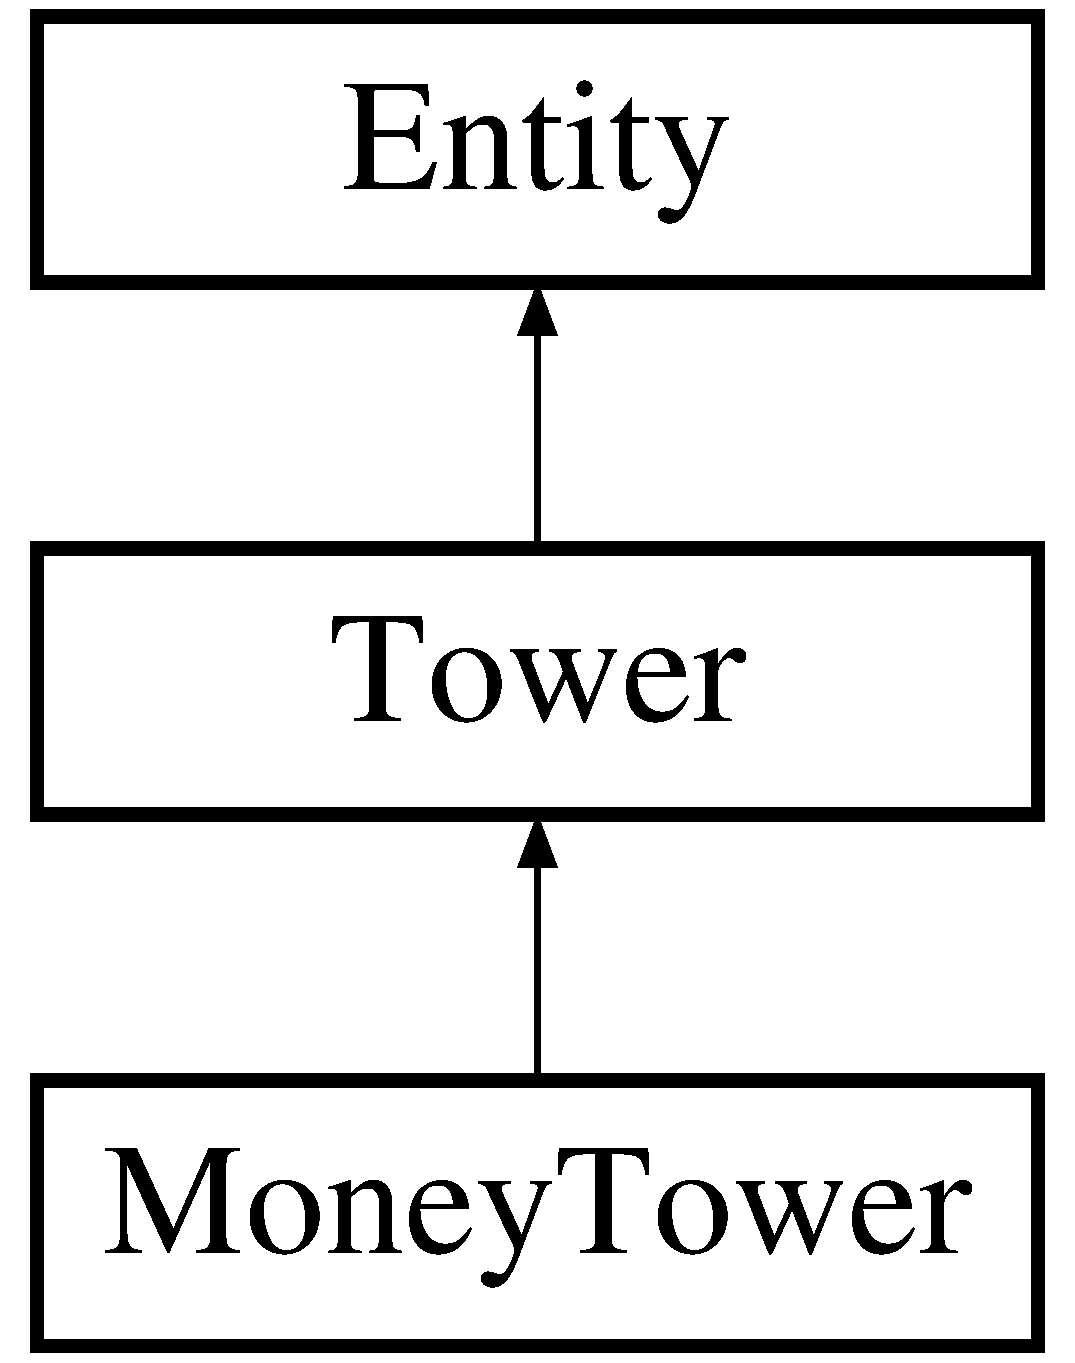
\includegraphics[height=3.000000cm]{class_money_tower}
\end{center}
\end{figure}
\subsection*{Public Member Functions}
\begin{DoxyCompactItemize}
\item 
\hyperlink{class_money_tower_a5c30b8e529f104ae8ab8d93392c27dd3}{Money\+Tower} (shared\+\_\+ptr$<$ \hyperlink{class_tile}{Tile} $>$ m\+Tile)
\item 
\hyperlink{class_money_tower_af35fe68ffc562a625aba39da5a07339a}{Money\+Tower} (float m\+Damage, int m\+Price, int m\+Level, float m\+Range, float m\+Speed, sf\+::\+Sprite m\+Sprite)
\item 
virtual \hyperlink{class_money_tower_abaa29f072ec89d2dfed4de83eb980122}{$\sim$\+Money\+Tower} ()
\item 
void \hyperlink{class_money_tower_a7bb3cc062e2d584247857f226283cf22}{generate\+Money} ()
\item 
void \hyperlink{class_money_tower_a83e66451e2e45ab85ffc2fa69ae79192}{do\+Attack} (sf\+::\+Render\+Window \&w) override
\end{DoxyCompactItemize}
\subsection*{Additional Inherited Members}


\subsection{Constructor \& Destructor Documentation}
\hypertarget{class_money_tower_a5c30b8e529f104ae8ab8d93392c27dd3}{\index{Money\+Tower@{Money\+Tower}!Money\+Tower@{Money\+Tower}}
\index{Money\+Tower@{Money\+Tower}!Money\+Tower@{Money\+Tower}}
\subsubsection[{Money\+Tower}]{\setlength{\rightskip}{0pt plus 5cm}Money\+Tower\+::\+Money\+Tower (
\begin{DoxyParamCaption}
\item[{shared\+\_\+ptr$<$ {\bf Tile} $>$}]{m\+Tile}
\end{DoxyParamCaption}
)}}\label{class_money_tower_a5c30b8e529f104ae8ab8d93392c27dd3}
\hypertarget{class_money_tower_af35fe68ffc562a625aba39da5a07339a}{\index{Money\+Tower@{Money\+Tower}!Money\+Tower@{Money\+Tower}}
\index{Money\+Tower@{Money\+Tower}!Money\+Tower@{Money\+Tower}}
\subsubsection[{Money\+Tower}]{\setlength{\rightskip}{0pt plus 5cm}Money\+Tower\+::\+Money\+Tower (
\begin{DoxyParamCaption}
\item[{float}]{m\+Damage, }
\item[{int}]{m\+Price, }
\item[{int}]{m\+Level, }
\item[{float}]{m\+Range, }
\item[{float}]{m\+Speed, }
\item[{sf\+::\+Sprite}]{m\+Sprite}
\end{DoxyParamCaption}
)}}\label{class_money_tower_af35fe68ffc562a625aba39da5a07339a}
\hypertarget{class_money_tower_abaa29f072ec89d2dfed4de83eb980122}{\index{Money\+Tower@{Money\+Tower}!````~Money\+Tower@{$\sim$\+Money\+Tower}}
\index{````~Money\+Tower@{$\sim$\+Money\+Tower}!Money\+Tower@{Money\+Tower}}
\subsubsection[{$\sim$\+Money\+Tower}]{\setlength{\rightskip}{0pt plus 5cm}virtual Money\+Tower\+::$\sim$\+Money\+Tower (
\begin{DoxyParamCaption}
{}
\end{DoxyParamCaption}
)\hspace{0.3cm}{\ttfamily [inline]}, {\ttfamily [virtual]}}}\label{class_money_tower_abaa29f072ec89d2dfed4de83eb980122}


\subsection{Member Function Documentation}
\hypertarget{class_money_tower_a83e66451e2e45ab85ffc2fa69ae79192}{\index{Money\+Tower@{Money\+Tower}!do\+Attack@{do\+Attack}}
\index{do\+Attack@{do\+Attack}!Money\+Tower@{Money\+Tower}}
\subsubsection[{do\+Attack}]{\setlength{\rightskip}{0pt plus 5cm}void Money\+Tower\+::do\+Attack (
\begin{DoxyParamCaption}
\item[{sf\+::\+Render\+Window \&}]{w}
\end{DoxyParamCaption}
)\hspace{0.3cm}{\ttfamily [override]}, {\ttfamily [virtual]}}}\label{class_money_tower_a83e66451e2e45ab85ffc2fa69ae79192}


Implements \hyperlink{class_tower_a24f01544e308e4b23650779867d54bf8}{Tower}.

\hypertarget{class_money_tower_a7bb3cc062e2d584247857f226283cf22}{\index{Money\+Tower@{Money\+Tower}!generate\+Money@{generate\+Money}}
\index{generate\+Money@{generate\+Money}!Money\+Tower@{Money\+Tower}}
\subsubsection[{generate\+Money}]{\setlength{\rightskip}{0pt plus 5cm}void Money\+Tower\+::generate\+Money (
\begin{DoxyParamCaption}
{}
\end{DoxyParamCaption}
)}}\label{class_money_tower_a7bb3cc062e2d584247857f226283cf22}


The documentation for this class was generated from the following files\+:\begin{DoxyCompactItemize}
\item 
D\+:/\+Tower\+Defense/\+Tower\+Defense/\hyperlink{_money_tower_8h}{Money\+Tower.\+h}\item 
D\+:/\+Tower\+Defense/\+Tower\+Defense/\hyperlink{_money_tower_8cpp}{Money\+Tower.\+cpp}\end{DoxyCompactItemize}

\hypertarget{class_normal_attack}{\section{Normal\+Attack Class Reference}
\label{class_normal_attack}\index{Normal\+Attack@{Normal\+Attack}}
}


{\ttfamily \#include $<$Normal\+Attack.\+h$>$}

Inheritance diagram for Normal\+Attack\+:\begin{figure}[H]
\begin{center}
\leavevmode
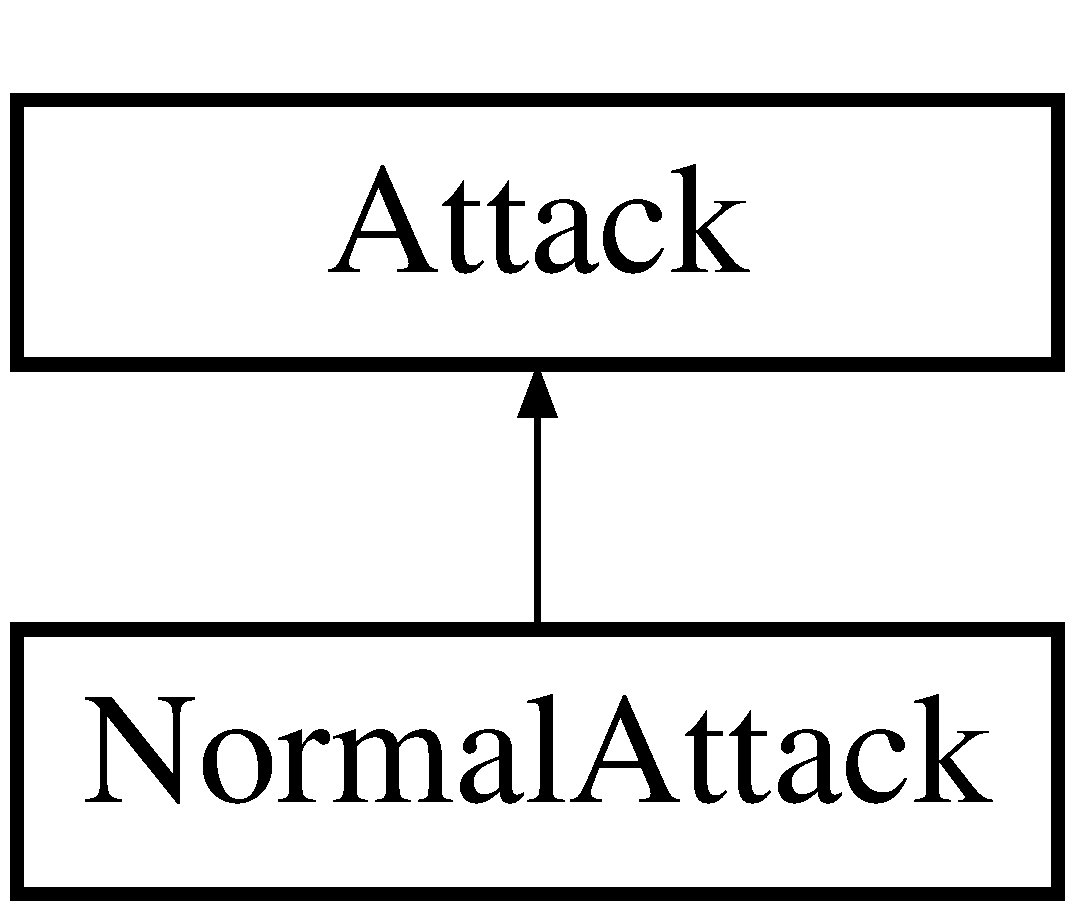
\includegraphics[height=2.000000cm]{class_normal_attack}
\end{center}
\end{figure}
\subsection*{Public Member Functions}
\begin{DoxyCompactItemize}
\item 
\hyperlink{class_normal_attack_a0570b31144ad70038827fb191c768b94}{Normal\+Attack} ()
\item 
virtual \hyperlink{class_normal_attack_a7dcfafca4da1344ed3aad0f0120d20ed}{$\sim$\+Normal\+Attack} ()
\item 
void \hyperlink{class_normal_attack_ae56877c3a110e0b4541776b89e252b10}{attack\+Animation} (sf\+::\+Render\+Window \&w) override
\item 
void \hyperlink{class_normal_attack_a949ea101fc201897cd3cd262b2870388}{resolve} (sf\+::\+Render\+Window \&w) override
\end{DoxyCompactItemize}
\subsection*{Additional Inherited Members}


\subsection{Constructor \& Destructor Documentation}
\hypertarget{class_normal_attack_a0570b31144ad70038827fb191c768b94}{\index{Normal\+Attack@{Normal\+Attack}!Normal\+Attack@{Normal\+Attack}}
\index{Normal\+Attack@{Normal\+Attack}!Normal\+Attack@{Normal\+Attack}}
\subsubsection[{Normal\+Attack}]{\setlength{\rightskip}{0pt plus 5cm}Normal\+Attack\+::\+Normal\+Attack (
\begin{DoxyParamCaption}
{}
\end{DoxyParamCaption}
)}}\label{class_normal_attack_a0570b31144ad70038827fb191c768b94}
\hypertarget{class_normal_attack_a7dcfafca4da1344ed3aad0f0120d20ed}{\index{Normal\+Attack@{Normal\+Attack}!````~Normal\+Attack@{$\sim$\+Normal\+Attack}}
\index{````~Normal\+Attack@{$\sim$\+Normal\+Attack}!Normal\+Attack@{Normal\+Attack}}
\subsubsection[{$\sim$\+Normal\+Attack}]{\setlength{\rightskip}{0pt plus 5cm}virtual Normal\+Attack\+::$\sim$\+Normal\+Attack (
\begin{DoxyParamCaption}
{}
\end{DoxyParamCaption}
)\hspace{0.3cm}{\ttfamily [inline]}, {\ttfamily [virtual]}}}\label{class_normal_attack_a7dcfafca4da1344ed3aad0f0120d20ed}


\subsection{Member Function Documentation}
\hypertarget{class_normal_attack_ae56877c3a110e0b4541776b89e252b10}{\index{Normal\+Attack@{Normal\+Attack}!attack\+Animation@{attack\+Animation}}
\index{attack\+Animation@{attack\+Animation}!Normal\+Attack@{Normal\+Attack}}
\subsubsection[{attack\+Animation}]{\setlength{\rightskip}{0pt plus 5cm}void Normal\+Attack\+::attack\+Animation (
\begin{DoxyParamCaption}
\item[{sf\+::\+Render\+Window \&}]{w}
\end{DoxyParamCaption}
)\hspace{0.3cm}{\ttfamily [override]}, {\ttfamily [virtual]}}}\label{class_normal_attack_ae56877c3a110e0b4541776b89e252b10}


Implements \hyperlink{class_attack_a893c5523d0c10531a99e0c84caf87ef6}{Attack}.

\hypertarget{class_normal_attack_a949ea101fc201897cd3cd262b2870388}{\index{Normal\+Attack@{Normal\+Attack}!resolve@{resolve}}
\index{resolve@{resolve}!Normal\+Attack@{Normal\+Attack}}
\subsubsection[{resolve}]{\setlength{\rightskip}{0pt plus 5cm}void Normal\+Attack\+::resolve (
\begin{DoxyParamCaption}
\item[{sf\+::\+Render\+Window \&}]{w}
\end{DoxyParamCaption}
)\hspace{0.3cm}{\ttfamily [override]}, {\ttfamily [virtual]}}}\label{class_normal_attack_a949ea101fc201897cd3cd262b2870388}


Implements \hyperlink{class_attack_aa3cd911d37e61278a9eeeb6d60303102}{Attack}.



The documentation for this class was generated from the following files\+:\begin{DoxyCompactItemize}
\item 
D\+:/\+Tower\+Defense/\+Tower\+Defense/\hyperlink{_normal_attack_8h}{Normal\+Attack.\+h}\item 
D\+:/\+Tower\+Defense/\+Tower\+Defense/\hyperlink{_normal_attack_8cpp}{Normal\+Attack.\+cpp}\end{DoxyCompactItemize}

\hypertarget{class_normal_enemy}{\section{Normal\+Enemy Class Reference}
\label{class_normal_enemy}\index{Normal\+Enemy@{Normal\+Enemy}}
}


{\ttfamily \#include $<$Normal\+Enemy.\+h$>$}

Inheritance diagram for Normal\+Enemy\+:\begin{figure}[H]
\begin{center}
\leavevmode
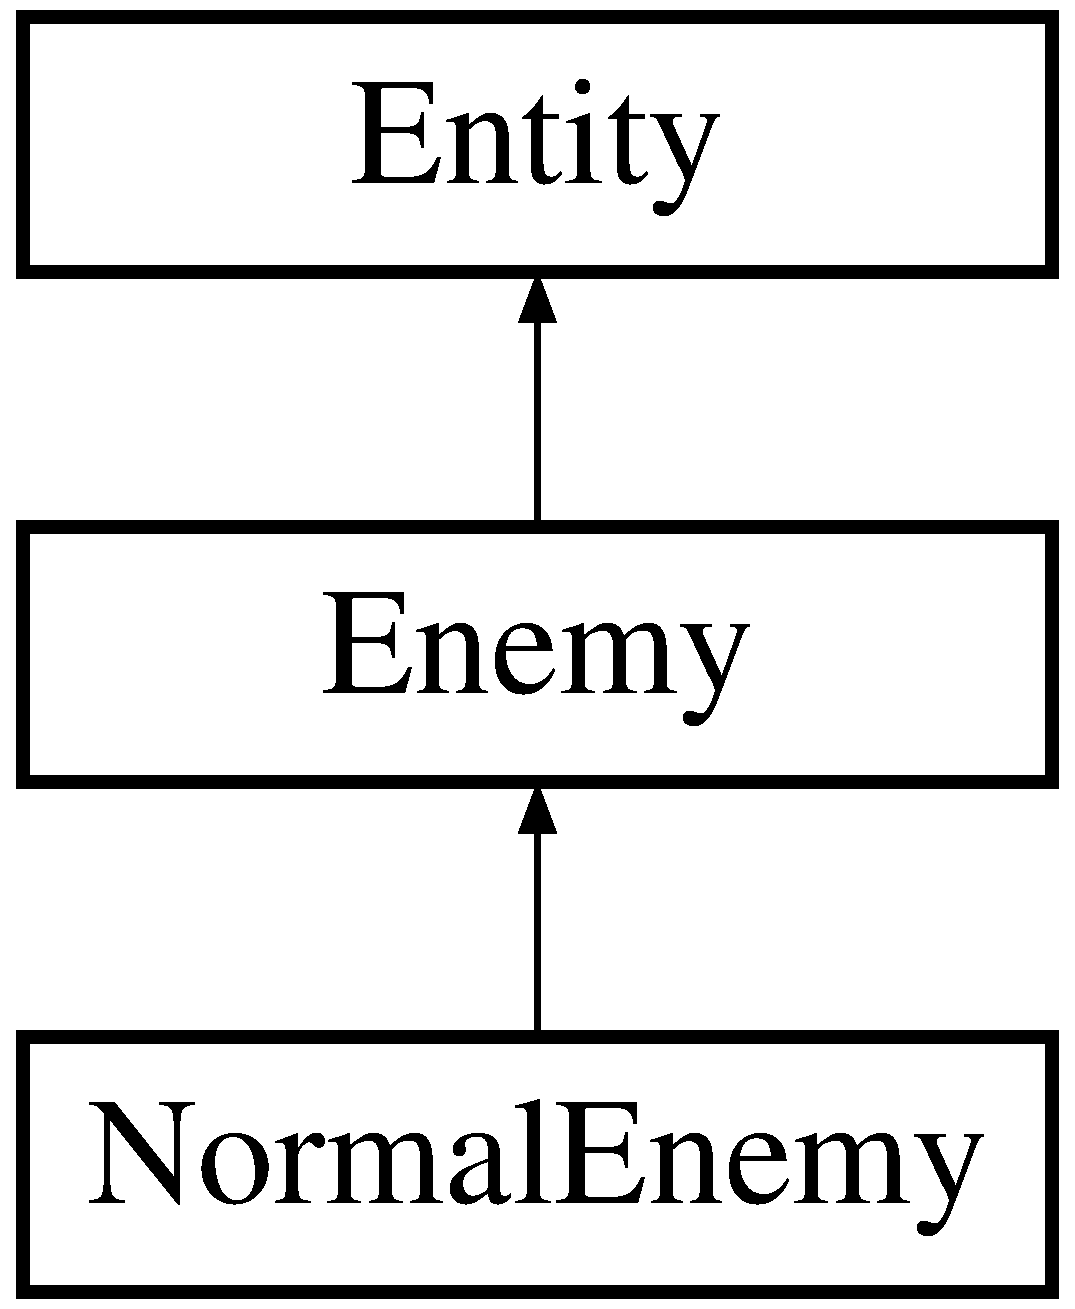
\includegraphics[height=3.000000cm]{class_normal_enemy}
\end{center}
\end{figure}
\subsection*{Public Member Functions}
\begin{DoxyCompactItemize}
\item 
\hyperlink{class_normal_enemy_aa386eea59a2983574fe7d55a91f93012}{Normal\+Enemy} ()
\item 
\hyperlink{class_normal_enemy_a078afb2bd89fb1036da05f604486a070}{Normal\+Enemy} (int \hyperlink{class_enemy_a278d70100af07c946743db1b7a1a9f59}{hp}, float \hyperlink{class_enemy_a9bb5d74024760e604c41ba79cc7da892}{defence}, int \hyperlink{class_enemy_a1d9a86d110b87f3cc55b40d1bdb59eb5}{bounty}, int \hyperlink{class_enemy_abc49d5a2cef917c8ece8a16547f8efee}{score\+Value}, sf\+::\+Sprite \hyperlink{class_entity_a48ef4ab143b8d0211877c9f6be42e824}{sprite}, float \hyperlink{class_entity_a1de3d8d9ab8088f61e6726069b26fa60}{speed})
\item 
virtual \hyperlink{class_normal_enemy_ab754d5476253062793eb7af3601785b6}{$\sim$\+Normal\+Enemy} ()
\item 
string \hyperlink{class_normal_enemy_a3409e903bc18e9ab9d58d8181ec6658f}{test} ()
\end{DoxyCompactItemize}
\subsection*{Additional Inherited Members}


\subsection{Constructor \& Destructor Documentation}
\hypertarget{class_normal_enemy_aa386eea59a2983574fe7d55a91f93012}{\index{Normal\+Enemy@{Normal\+Enemy}!Normal\+Enemy@{Normal\+Enemy}}
\index{Normal\+Enemy@{Normal\+Enemy}!Normal\+Enemy@{Normal\+Enemy}}
\subsubsection[{Normal\+Enemy}]{\setlength{\rightskip}{0pt plus 5cm}Normal\+Enemy\+::\+Normal\+Enemy (
\begin{DoxyParamCaption}
{}
\end{DoxyParamCaption}
)}}\label{class_normal_enemy_aa386eea59a2983574fe7d55a91f93012}
\hypertarget{class_normal_enemy_a078afb2bd89fb1036da05f604486a070}{\index{Normal\+Enemy@{Normal\+Enemy}!Normal\+Enemy@{Normal\+Enemy}}
\index{Normal\+Enemy@{Normal\+Enemy}!Normal\+Enemy@{Normal\+Enemy}}
\subsubsection[{Normal\+Enemy}]{\setlength{\rightskip}{0pt plus 5cm}Normal\+Enemy\+::\+Normal\+Enemy (
\begin{DoxyParamCaption}
\item[{int}]{hp, }
\item[{float}]{defence, }
\item[{int}]{bounty, }
\item[{int}]{score\+Value, }
\item[{sf\+::\+Sprite}]{sprite, }
\item[{float}]{speed}
\end{DoxyParamCaption}
)}}\label{class_normal_enemy_a078afb2bd89fb1036da05f604486a070}
\hypertarget{class_normal_enemy_ab754d5476253062793eb7af3601785b6}{\index{Normal\+Enemy@{Normal\+Enemy}!````~Normal\+Enemy@{$\sim$\+Normal\+Enemy}}
\index{````~Normal\+Enemy@{$\sim$\+Normal\+Enemy}!Normal\+Enemy@{Normal\+Enemy}}
\subsubsection[{$\sim$\+Normal\+Enemy}]{\setlength{\rightskip}{0pt plus 5cm}virtual Normal\+Enemy\+::$\sim$\+Normal\+Enemy (
\begin{DoxyParamCaption}
{}
\end{DoxyParamCaption}
)\hspace{0.3cm}{\ttfamily [inline]}, {\ttfamily [virtual]}}}\label{class_normal_enemy_ab754d5476253062793eb7af3601785b6}


\subsection{Member Function Documentation}
\hypertarget{class_normal_enemy_a3409e903bc18e9ab9d58d8181ec6658f}{\index{Normal\+Enemy@{Normal\+Enemy}!test@{test}}
\index{test@{test}!Normal\+Enemy@{Normal\+Enemy}}
\subsubsection[{test}]{\setlength{\rightskip}{0pt plus 5cm}string Normal\+Enemy\+::test (
\begin{DoxyParamCaption}
{}
\end{DoxyParamCaption}
)\hspace{0.3cm}{\ttfamily [inline]}, {\ttfamily [virtual]}}}\label{class_normal_enemy_a3409e903bc18e9ab9d58d8181ec6658f}


Implements \hyperlink{class_enemy_a37b2bae4f5a9e8d673aeb28880ded0bc}{Enemy}.



The documentation for this class was generated from the following files\+:\begin{DoxyCompactItemize}
\item 
D\+:/\+Tower\+Defense/\+Tower\+Defense/\hyperlink{_normal_enemy_8h}{Normal\+Enemy.\+h}\item 
D\+:/\+Tower\+Defense/\+Tower\+Defense/\hyperlink{_normal_enemy_8cpp}{Normal\+Enemy.\+cpp}\end{DoxyCompactItemize}

\hypertarget{class_normal_tower}{\section{Normal\+Tower Class Reference}
\label{class_normal_tower}\index{Normal\+Tower@{Normal\+Tower}}
}


{\ttfamily \#include $<$Normal\+Tower.\+h$>$}

Inheritance diagram for Normal\+Tower\+:\begin{figure}[H]
\begin{center}
\leavevmode
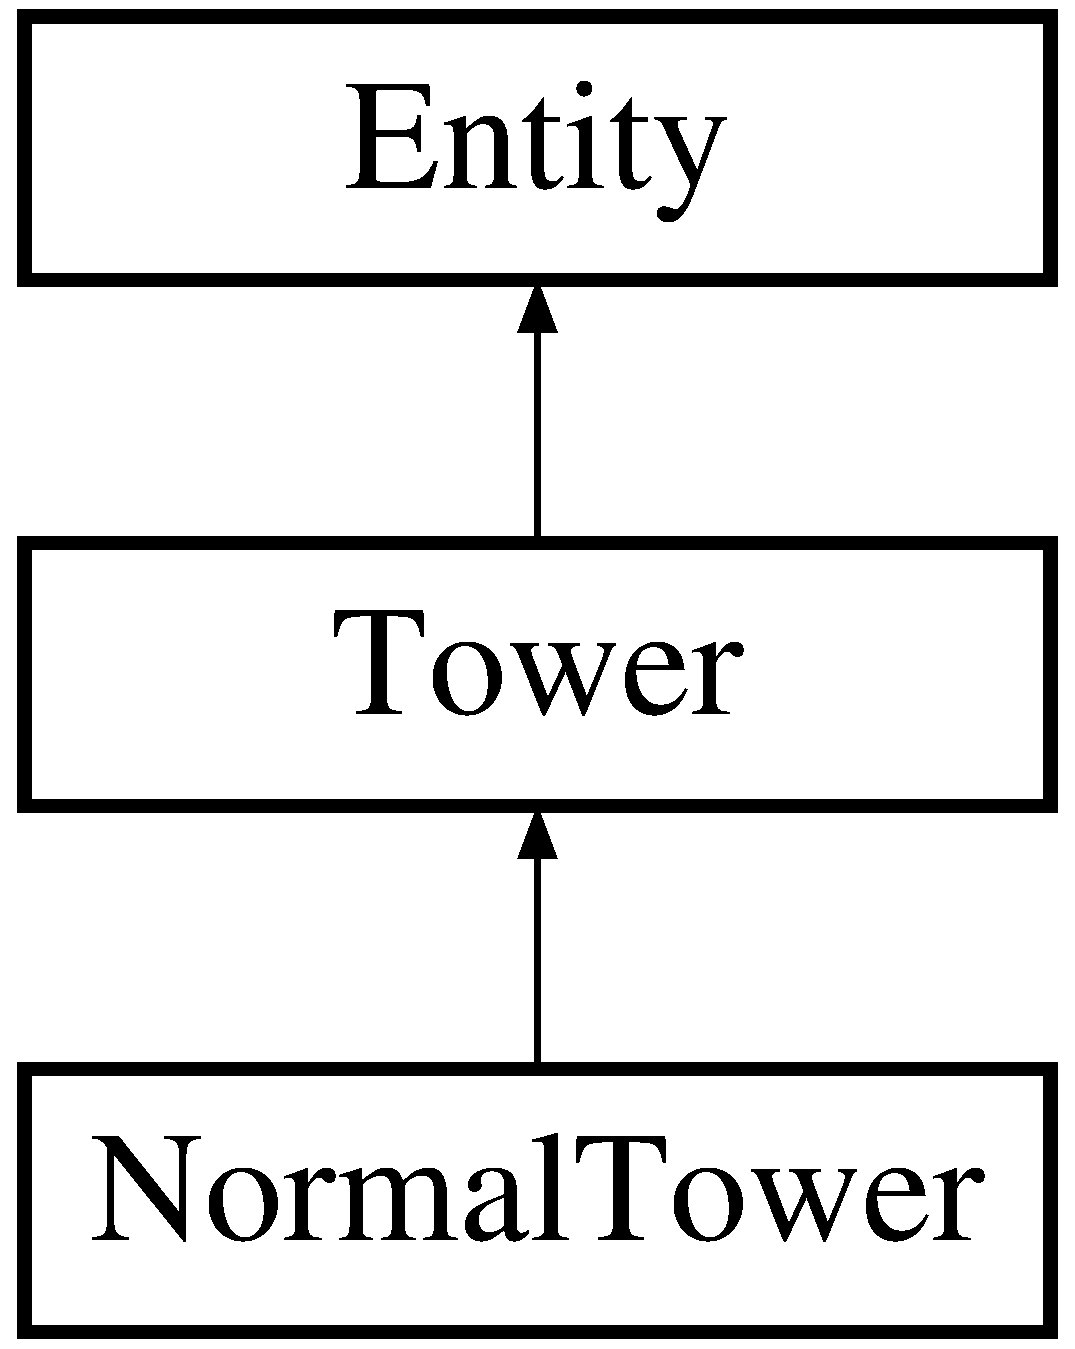
\includegraphics[height=3.000000cm]{class_normal_tower}
\end{center}
\end{figure}
\subsection*{Public Member Functions}
\begin{DoxyCompactItemize}
\item 
\hyperlink{class_normal_tower_a99db5d3dbf58cd6ba3619d4e4601630c}{Normal\+Tower} (shared\+\_\+ptr$<$ \hyperlink{class_tile}{Tile} $>$ m\+Tile)
\item 
\hyperlink{class_normal_tower_a9f7b920d45d9b3388d0039ecf5febbd3}{Normal\+Tower} (float m\+Damage, int m\+Price, int m\+Level, float m\+Range, float m\+Speed, sf\+::\+Sprite m\+Sprite)
\item 
virtual \hyperlink{class_normal_tower_a26761e67765db3cdb854c695d17b7bc5}{$\sim$\+Normal\+Tower} ()
\item 
void \hyperlink{class_normal_tower_a1e3b0a2216d943650b060bac297511b6}{do\+Attack} (sf\+::\+Render\+Window \&w) override
\end{DoxyCompactItemize}
\subsection*{Additional Inherited Members}


\subsection{Constructor \& Destructor Documentation}
\hypertarget{class_normal_tower_a99db5d3dbf58cd6ba3619d4e4601630c}{\index{Normal\+Tower@{Normal\+Tower}!Normal\+Tower@{Normal\+Tower}}
\index{Normal\+Tower@{Normal\+Tower}!Normal\+Tower@{Normal\+Tower}}
\subsubsection[{Normal\+Tower}]{\setlength{\rightskip}{0pt plus 5cm}Normal\+Tower\+::\+Normal\+Tower (
\begin{DoxyParamCaption}
\item[{shared\+\_\+ptr$<$ {\bf Tile} $>$}]{m\+Tile}
\end{DoxyParamCaption}
)}}\label{class_normal_tower_a99db5d3dbf58cd6ba3619d4e4601630c}
\hypertarget{class_normal_tower_a9f7b920d45d9b3388d0039ecf5febbd3}{\index{Normal\+Tower@{Normal\+Tower}!Normal\+Tower@{Normal\+Tower}}
\index{Normal\+Tower@{Normal\+Tower}!Normal\+Tower@{Normal\+Tower}}
\subsubsection[{Normal\+Tower}]{\setlength{\rightskip}{0pt plus 5cm}Normal\+Tower\+::\+Normal\+Tower (
\begin{DoxyParamCaption}
\item[{float}]{m\+Damage, }
\item[{int}]{m\+Price, }
\item[{int}]{m\+Level, }
\item[{float}]{m\+Range, }
\item[{float}]{m\+Speed, }
\item[{sf\+::\+Sprite}]{m\+Sprite}
\end{DoxyParamCaption}
)}}\label{class_normal_tower_a9f7b920d45d9b3388d0039ecf5febbd3}
\hypertarget{class_normal_tower_a26761e67765db3cdb854c695d17b7bc5}{\index{Normal\+Tower@{Normal\+Tower}!````~Normal\+Tower@{$\sim$\+Normal\+Tower}}
\index{````~Normal\+Tower@{$\sim$\+Normal\+Tower}!Normal\+Tower@{Normal\+Tower}}
\subsubsection[{$\sim$\+Normal\+Tower}]{\setlength{\rightskip}{0pt plus 5cm}virtual Normal\+Tower\+::$\sim$\+Normal\+Tower (
\begin{DoxyParamCaption}
{}
\end{DoxyParamCaption}
)\hspace{0.3cm}{\ttfamily [inline]}, {\ttfamily [virtual]}}}\label{class_normal_tower_a26761e67765db3cdb854c695d17b7bc5}


\subsection{Member Function Documentation}
\hypertarget{class_normal_tower_a1e3b0a2216d943650b060bac297511b6}{\index{Normal\+Tower@{Normal\+Tower}!do\+Attack@{do\+Attack}}
\index{do\+Attack@{do\+Attack}!Normal\+Tower@{Normal\+Tower}}
\subsubsection[{do\+Attack}]{\setlength{\rightskip}{0pt plus 5cm}void Normal\+Tower\+::do\+Attack (
\begin{DoxyParamCaption}
\item[{sf\+::\+Render\+Window \&}]{w}
\end{DoxyParamCaption}
)\hspace{0.3cm}{\ttfamily [override]}, {\ttfamily [virtual]}}}\label{class_normal_tower_a1e3b0a2216d943650b060bac297511b6}


Implements \hyperlink{class_tower_a24f01544e308e4b23650779867d54bf8}{Tower}.



The documentation for this class was generated from the following files\+:\begin{DoxyCompactItemize}
\item 
D\+:/\+Tower\+Defense/\+Tower\+Defense/\hyperlink{_normal_tower_8h}{Normal\+Tower.\+h}\item 
D\+:/\+Tower\+Defense/\+Tower\+Defense/\hyperlink{_normal_tower_8cpp}{Normal\+Tower.\+cpp}\end{DoxyCompactItemize}

\hypertarget{class_path}{\section{Path Class Reference}
\label{class_path}\index{Path@{Path}}
}


{\ttfamily \#include $<$Path.\+h$>$}

\subsection*{Public Member Functions}
\begin{DoxyCompactItemize}
\item 
void \hyperlink{class_path_a6d7187d9ef0f353f336d64e5244b0b76}{draw} (sf\+::\+Render\+Window \&)
\item 
\hyperlink{class_path_a861c8f51e8428a7a2960a2f9a75beb28}{Path} (vector$<$ shared\+\_\+ptr$<$ \hyperlink{class_tile}{Tile} $>$$>$)
\item 
\hyperlink{class_path_af26cfab021ddf49af73da3b2beca85ac}{Path} ()
\item 
vector$<$ shared\+\_\+ptr$<$ \hyperlink{class_tile}{Tile} $>$ $>$ \hyperlink{class_path_aca110b8b269cae3f65f80c49059d6492}{get\+Path} ()
\end{DoxyCompactItemize}


\subsection{Constructor \& Destructor Documentation}
\hypertarget{class_path_a861c8f51e8428a7a2960a2f9a75beb28}{\index{Path@{Path}!Path@{Path}}
\index{Path@{Path}!Path@{Path}}
\subsubsection[{Path}]{\setlength{\rightskip}{0pt plus 5cm}Path\+::\+Path (
\begin{DoxyParamCaption}
\item[{vector$<$ shared\+\_\+ptr$<$ {\bf Tile} $>$$>$}]{a}
\end{DoxyParamCaption}
)}}\label{class_path_a861c8f51e8428a7a2960a2f9a75beb28}
\hypertarget{class_path_af26cfab021ddf49af73da3b2beca85ac}{\index{Path@{Path}!Path@{Path}}
\index{Path@{Path}!Path@{Path}}
\subsubsection[{Path}]{\setlength{\rightskip}{0pt plus 5cm}Path\+::\+Path (
\begin{DoxyParamCaption}
{}
\end{DoxyParamCaption}
)}}\label{class_path_af26cfab021ddf49af73da3b2beca85ac}


\subsection{Member Function Documentation}
\hypertarget{class_path_a6d7187d9ef0f353f336d64e5244b0b76}{\index{Path@{Path}!draw@{draw}}
\index{draw@{draw}!Path@{Path}}
\subsubsection[{draw}]{\setlength{\rightskip}{0pt plus 5cm}void Path\+::draw (
\begin{DoxyParamCaption}
\item[{sf\+::\+Render\+Window \&}]{w}
\end{DoxyParamCaption}
)}}\label{class_path_a6d7187d9ef0f353f336d64e5244b0b76}
\hypertarget{class_path_aca110b8b269cae3f65f80c49059d6492}{\index{Path@{Path}!get\+Path@{get\+Path}}
\index{get\+Path@{get\+Path}!Path@{Path}}
\subsubsection[{get\+Path}]{\setlength{\rightskip}{0pt plus 5cm}vector$<$ shared\+\_\+ptr$<$ {\bf Tile} $>$ $>$ Path\+::get\+Path (
\begin{DoxyParamCaption}
{}
\end{DoxyParamCaption}
)}}\label{class_path_aca110b8b269cae3f65f80c49059d6492}


The documentation for this class was generated from the following files\+:\begin{DoxyCompactItemize}
\item 
D\+:/\+Tower\+Defense/\+Tower\+Defense/\hyperlink{_path_8h}{Path.\+h}\item 
D\+:/\+Tower\+Defense/\+Tower\+Defense/\hyperlink{_path_8cpp}{Path.\+cpp}\end{DoxyCompactItemize}

\hypertarget{class_player}{\section{Player Class Reference}
\label{class_player}\index{Player@{Player}}
}


{\ttfamily \#include $<$Player.\+h$>$}

\subsection*{Public Member Functions}
\begin{DoxyCompactItemize}
\item 
\hyperlink{class_player_affe0cc3cb714f6deb4e62f0c0d3f1fd8}{Player} ()
\item 
void \hyperlink{class_player_ae1969eb6823abda215454eba0e57fbf1}{manage\+Money} (int)
\item 
void \hyperlink{class_player_adaa8a60e604c08eeb43ac222d6bbe0f0}{manage\+Score} (int)
\item 
void \hyperlink{class_player_afe6e5a3b4455aac2a27619a98115f14e}{manage\+H\+P} (int)
\item 
int \hyperlink{class_player_ab48412e49754288ddff1e4568ecd63b5}{get\+H\+P} ()
\item 
int \hyperlink{class_player_a97e5447778ae6c384eedc532dcd8431d}{get\+Score} ()
\item 
int \hyperlink{class_player_ac45154df7c4eb2d1d58255c3ff1c55dd}{get\+Money} ()
\item 
void \hyperlink{class_player_a015ea21fa1e7273e47d48cb20d9b12e3}{init} ()
\end{DoxyCompactItemize}


\subsection{Constructor \& Destructor Documentation}
\hypertarget{class_player_affe0cc3cb714f6deb4e62f0c0d3f1fd8}{\index{Player@{Player}!Player@{Player}}
\index{Player@{Player}!Player@{Player}}
\subsubsection[{Player}]{\setlength{\rightskip}{0pt plus 5cm}Player\+::\+Player (
\begin{DoxyParamCaption}
{}
\end{DoxyParamCaption}
)}}\label{class_player_affe0cc3cb714f6deb4e62f0c0d3f1fd8}


\subsection{Member Function Documentation}
\hypertarget{class_player_ab48412e49754288ddff1e4568ecd63b5}{\index{Player@{Player}!get\+H\+P@{get\+H\+P}}
\index{get\+H\+P@{get\+H\+P}!Player@{Player}}
\subsubsection[{get\+H\+P}]{\setlength{\rightskip}{0pt plus 5cm}int Player\+::get\+H\+P (
\begin{DoxyParamCaption}
{}
\end{DoxyParamCaption}
)}}\label{class_player_ab48412e49754288ddff1e4568ecd63b5}
\hypertarget{class_player_ac45154df7c4eb2d1d58255c3ff1c55dd}{\index{Player@{Player}!get\+Money@{get\+Money}}
\index{get\+Money@{get\+Money}!Player@{Player}}
\subsubsection[{get\+Money}]{\setlength{\rightskip}{0pt plus 5cm}int Player\+::get\+Money (
\begin{DoxyParamCaption}
{}
\end{DoxyParamCaption}
)}}\label{class_player_ac45154df7c4eb2d1d58255c3ff1c55dd}
\hypertarget{class_player_a97e5447778ae6c384eedc532dcd8431d}{\index{Player@{Player}!get\+Score@{get\+Score}}
\index{get\+Score@{get\+Score}!Player@{Player}}
\subsubsection[{get\+Score}]{\setlength{\rightskip}{0pt plus 5cm}int Player\+::get\+Score (
\begin{DoxyParamCaption}
{}
\end{DoxyParamCaption}
)}}\label{class_player_a97e5447778ae6c384eedc532dcd8431d}
\hypertarget{class_player_a015ea21fa1e7273e47d48cb20d9b12e3}{\index{Player@{Player}!init@{init}}
\index{init@{init}!Player@{Player}}
\subsubsection[{init}]{\setlength{\rightskip}{0pt plus 5cm}void Player\+::init (
\begin{DoxyParamCaption}
{}
\end{DoxyParamCaption}
)}}\label{class_player_a015ea21fa1e7273e47d48cb20d9b12e3}
\hypertarget{class_player_afe6e5a3b4455aac2a27619a98115f14e}{\index{Player@{Player}!manage\+H\+P@{manage\+H\+P}}
\index{manage\+H\+P@{manage\+H\+P}!Player@{Player}}
\subsubsection[{manage\+H\+P}]{\setlength{\rightskip}{0pt plus 5cm}void Player\+::manage\+H\+P (
\begin{DoxyParamCaption}
\item[{int}]{h}
\end{DoxyParamCaption}
)}}\label{class_player_afe6e5a3b4455aac2a27619a98115f14e}
\hypertarget{class_player_ae1969eb6823abda215454eba0e57fbf1}{\index{Player@{Player}!manage\+Money@{manage\+Money}}
\index{manage\+Money@{manage\+Money}!Player@{Player}}
\subsubsection[{manage\+Money}]{\setlength{\rightskip}{0pt plus 5cm}void Player\+::manage\+Money (
\begin{DoxyParamCaption}
\item[{int}]{m}
\end{DoxyParamCaption}
)}}\label{class_player_ae1969eb6823abda215454eba0e57fbf1}
\hypertarget{class_player_adaa8a60e604c08eeb43ac222d6bbe0f0}{\index{Player@{Player}!manage\+Score@{manage\+Score}}
\index{manage\+Score@{manage\+Score}!Player@{Player}}
\subsubsection[{manage\+Score}]{\setlength{\rightskip}{0pt plus 5cm}void Player\+::manage\+Score (
\begin{DoxyParamCaption}
\item[{int}]{s}
\end{DoxyParamCaption}
)}}\label{class_player_adaa8a60e604c08eeb43ac222d6bbe0f0}


The documentation for this class was generated from the following files\+:\begin{DoxyCompactItemize}
\item 
D\+:/\+Tower\+Defense/\+Tower\+Defense/\hyperlink{_player_8h}{Player.\+h}\item 
D\+:/\+Tower\+Defense/\+Tower\+Defense/\hyperlink{_player_8cpp}{Player.\+cpp}\end{DoxyCompactItemize}

\hypertarget{class_slow_attack}{\section{Slow\+Attack Class Reference}
\label{class_slow_attack}\index{Slow\+Attack@{Slow\+Attack}}
}


{\ttfamily \#include $<$Slow\+Attack.\+h$>$}

Inheritance diagram for Slow\+Attack\+:\begin{figure}[H]
\begin{center}
\leavevmode
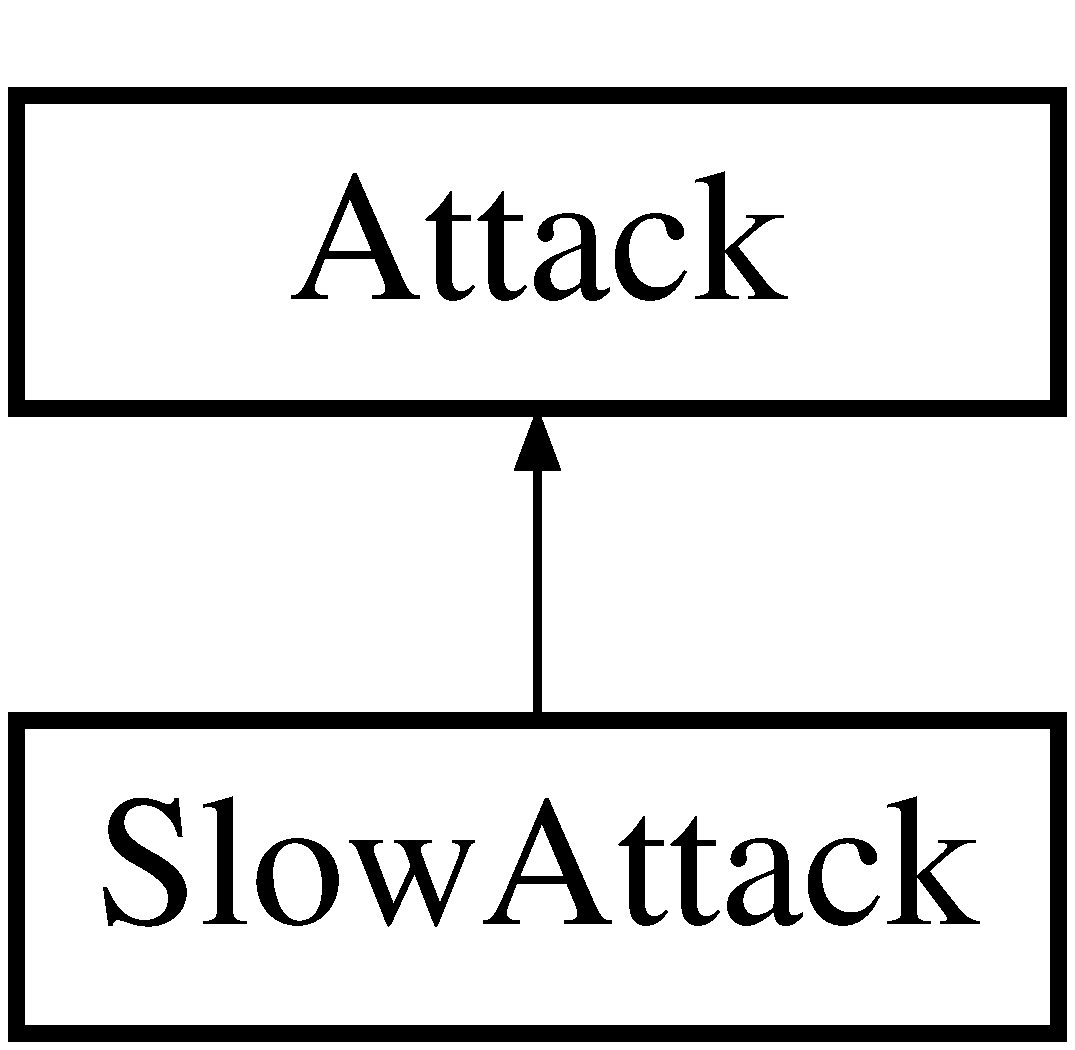
\includegraphics[height=2.000000cm]{class_slow_attack}
\end{center}
\end{figure}
\subsection*{Public Member Functions}
\begin{DoxyCompactItemize}
\item 
\hyperlink{class_slow_attack_ae00c267aa1ef2822860027cb33e12c79}{Slow\+Attack} ()
\item 
virtual \hyperlink{class_slow_attack_ac58dc4cbd28056655d5b005fda0fc562}{$\sim$\+Slow\+Attack} ()
\item 
void \hyperlink{class_slow_attack_afa5a9af6a5b26bdb4168ee5a909433a6}{attack\+Animation} (sf\+::\+Render\+Window \&w) override
\item 
void \hyperlink{class_slow_attack_a73767803482c26adf9aae486faa7499c}{resolve} (sf\+::\+Render\+Window \&w) override
\end{DoxyCompactItemize}
\subsection*{Additional Inherited Members}


\subsection{Constructor \& Destructor Documentation}
\hypertarget{class_slow_attack_ae00c267aa1ef2822860027cb33e12c79}{\index{Slow\+Attack@{Slow\+Attack}!Slow\+Attack@{Slow\+Attack}}
\index{Slow\+Attack@{Slow\+Attack}!Slow\+Attack@{Slow\+Attack}}
\subsubsection[{Slow\+Attack}]{\setlength{\rightskip}{0pt plus 5cm}Slow\+Attack\+::\+Slow\+Attack (
\begin{DoxyParamCaption}
{}
\end{DoxyParamCaption}
)}}\label{class_slow_attack_ae00c267aa1ef2822860027cb33e12c79}
\hypertarget{class_slow_attack_ac58dc4cbd28056655d5b005fda0fc562}{\index{Slow\+Attack@{Slow\+Attack}!````~Slow\+Attack@{$\sim$\+Slow\+Attack}}
\index{````~Slow\+Attack@{$\sim$\+Slow\+Attack}!Slow\+Attack@{Slow\+Attack}}
\subsubsection[{$\sim$\+Slow\+Attack}]{\setlength{\rightskip}{0pt plus 5cm}virtual Slow\+Attack\+::$\sim$\+Slow\+Attack (
\begin{DoxyParamCaption}
{}
\end{DoxyParamCaption}
)\hspace{0.3cm}{\ttfamily [inline]}, {\ttfamily [virtual]}}}\label{class_slow_attack_ac58dc4cbd28056655d5b005fda0fc562}


\subsection{Member Function Documentation}
\hypertarget{class_slow_attack_afa5a9af6a5b26bdb4168ee5a909433a6}{\index{Slow\+Attack@{Slow\+Attack}!attack\+Animation@{attack\+Animation}}
\index{attack\+Animation@{attack\+Animation}!Slow\+Attack@{Slow\+Attack}}
\subsubsection[{attack\+Animation}]{\setlength{\rightskip}{0pt plus 5cm}void Slow\+Attack\+::attack\+Animation (
\begin{DoxyParamCaption}
\item[{sf\+::\+Render\+Window \&}]{w}
\end{DoxyParamCaption}
)\hspace{0.3cm}{\ttfamily [override]}, {\ttfamily [virtual]}}}\label{class_slow_attack_afa5a9af6a5b26bdb4168ee5a909433a6}


Implements \hyperlink{class_attack_a893c5523d0c10531a99e0c84caf87ef6}{Attack}.

\hypertarget{class_slow_attack_a73767803482c26adf9aae486faa7499c}{\index{Slow\+Attack@{Slow\+Attack}!resolve@{resolve}}
\index{resolve@{resolve}!Slow\+Attack@{Slow\+Attack}}
\subsubsection[{resolve}]{\setlength{\rightskip}{0pt plus 5cm}void Slow\+Attack\+::resolve (
\begin{DoxyParamCaption}
\item[{sf\+::\+Render\+Window \&}]{w}
\end{DoxyParamCaption}
)\hspace{0.3cm}{\ttfamily [override]}, {\ttfamily [virtual]}}}\label{class_slow_attack_a73767803482c26adf9aae486faa7499c}


Implements \hyperlink{class_attack_aa3cd911d37e61278a9eeeb6d60303102}{Attack}.



The documentation for this class was generated from the following files\+:\begin{DoxyCompactItemize}
\item 
D\+:/\+Tower\+Defense/\+Tower\+Defense/\hyperlink{_slow_attack_8h}{Slow\+Attack.\+h}\item 
D\+:/\+Tower\+Defense/\+Tower\+Defense/\hyperlink{_slow_attack_8cpp}{Slow\+Attack.\+cpp}\end{DoxyCompactItemize}

\hypertarget{class_slow_tower}{\section{Slow\+Tower Class Reference}
\label{class_slow_tower}\index{Slow\+Tower@{Slow\+Tower}}
}


{\ttfamily \#include $<$Slow\+Tower.\+h$>$}

Inheritance diagram for Slow\+Tower\+:\begin{figure}[H]
\begin{center}
\leavevmode
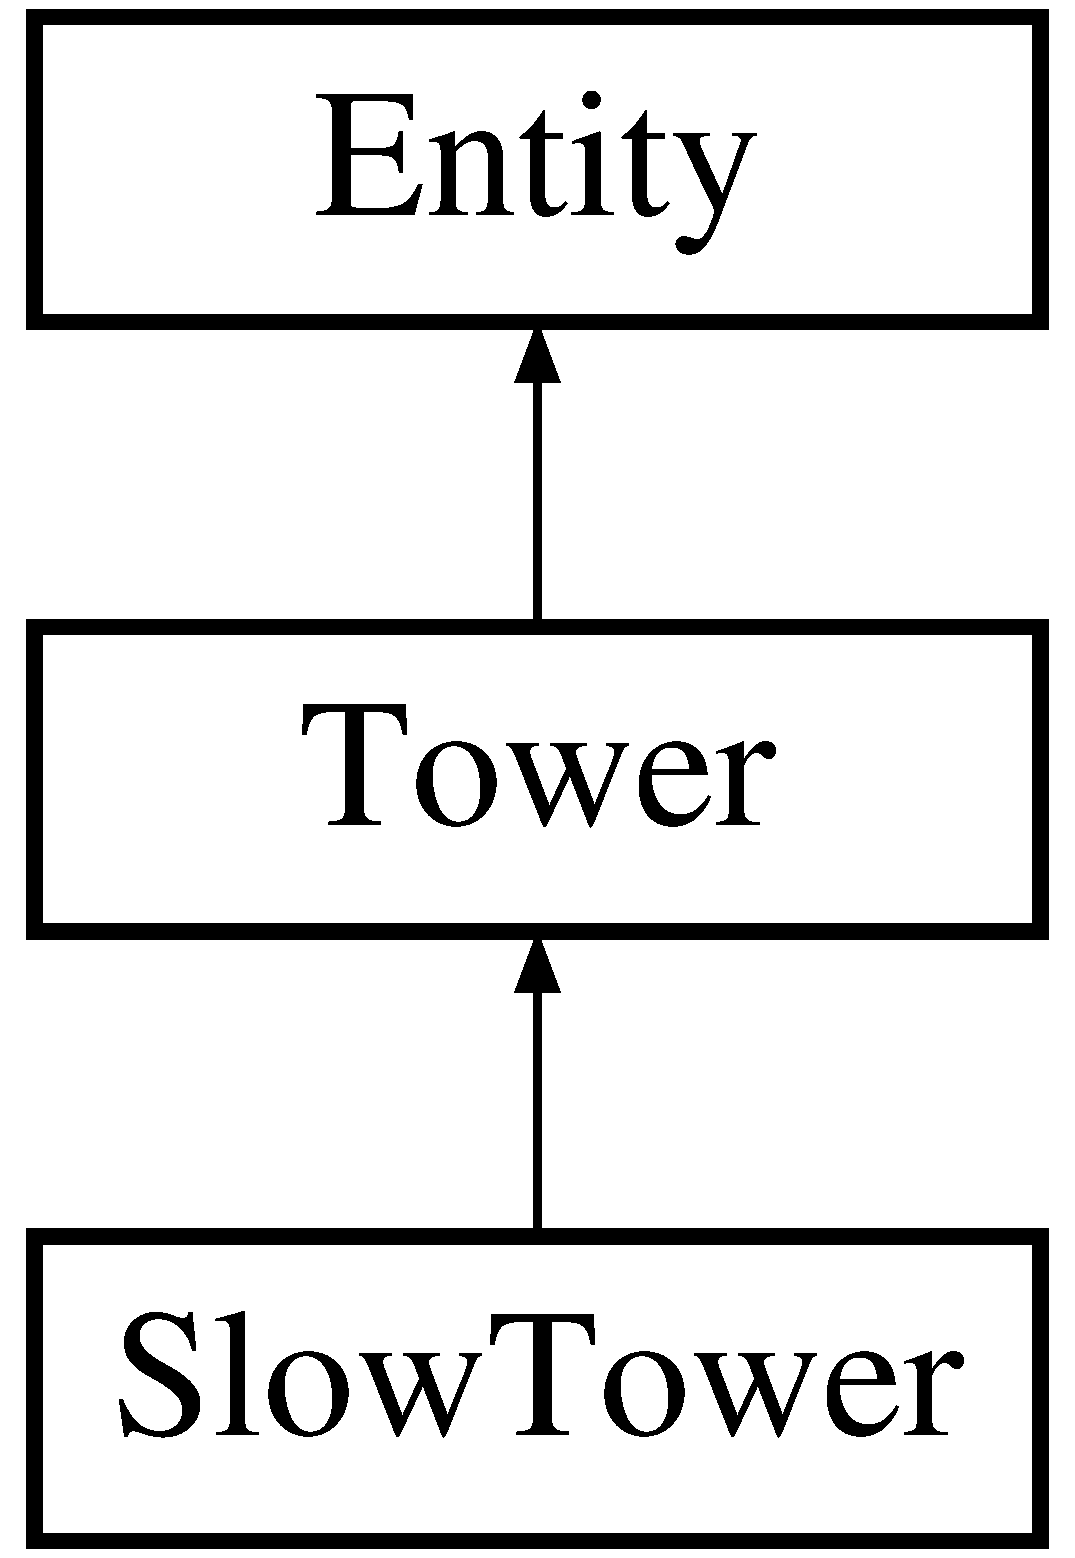
\includegraphics[height=3.000000cm]{class_slow_tower}
\end{center}
\end{figure}
\subsection*{Public Member Functions}
\begin{DoxyCompactItemize}
\item 
\hyperlink{class_slow_tower_a05ce0356b1d846450e3c522d5558974f}{Slow\+Tower} (shared\+\_\+ptr$<$ \hyperlink{class_tile}{Tile} $>$ m\+Tile)
\item 
\hyperlink{class_slow_tower_af7681fbf8310e36d9933ad0f76747958}{Slow\+Tower} (float m\+Damage, int m\+Price, int m\+Level, float m\+Range, float m\+Speed, sf\+::\+Sprite m\+Sprite)
\item 
virtual \hyperlink{class_slow_tower_ab0401cca62dc2cff530fe29e5a6baed9}{$\sim$\+Slow\+Tower} ()
\item 
void \hyperlink{class_slow_tower_a263531cb94fccecfdc1bd667a54b168d}{do\+Attack} (sf\+::\+Render\+Window \&w) override
\end{DoxyCompactItemize}
\subsection*{Additional Inherited Members}


\subsection{Constructor \& Destructor Documentation}
\hypertarget{class_slow_tower_a05ce0356b1d846450e3c522d5558974f}{\index{Slow\+Tower@{Slow\+Tower}!Slow\+Tower@{Slow\+Tower}}
\index{Slow\+Tower@{Slow\+Tower}!Slow\+Tower@{Slow\+Tower}}
\subsubsection[{Slow\+Tower}]{\setlength{\rightskip}{0pt plus 5cm}Slow\+Tower\+::\+Slow\+Tower (
\begin{DoxyParamCaption}
\item[{shared\+\_\+ptr$<$ {\bf Tile} $>$}]{m\+Tile}
\end{DoxyParamCaption}
)}}\label{class_slow_tower_a05ce0356b1d846450e3c522d5558974f}
\hypertarget{class_slow_tower_af7681fbf8310e36d9933ad0f76747958}{\index{Slow\+Tower@{Slow\+Tower}!Slow\+Tower@{Slow\+Tower}}
\index{Slow\+Tower@{Slow\+Tower}!Slow\+Tower@{Slow\+Tower}}
\subsubsection[{Slow\+Tower}]{\setlength{\rightskip}{0pt plus 5cm}Slow\+Tower\+::\+Slow\+Tower (
\begin{DoxyParamCaption}
\item[{float}]{m\+Damage, }
\item[{int}]{m\+Price, }
\item[{int}]{m\+Level, }
\item[{float}]{m\+Range, }
\item[{float}]{m\+Speed, }
\item[{sf\+::\+Sprite}]{m\+Sprite}
\end{DoxyParamCaption}
)}}\label{class_slow_tower_af7681fbf8310e36d9933ad0f76747958}
\hypertarget{class_slow_tower_ab0401cca62dc2cff530fe29e5a6baed9}{\index{Slow\+Tower@{Slow\+Tower}!````~Slow\+Tower@{$\sim$\+Slow\+Tower}}
\index{````~Slow\+Tower@{$\sim$\+Slow\+Tower}!Slow\+Tower@{Slow\+Tower}}
\subsubsection[{$\sim$\+Slow\+Tower}]{\setlength{\rightskip}{0pt plus 5cm}virtual Slow\+Tower\+::$\sim$\+Slow\+Tower (
\begin{DoxyParamCaption}
{}
\end{DoxyParamCaption}
)\hspace{0.3cm}{\ttfamily [inline]}, {\ttfamily [virtual]}}}\label{class_slow_tower_ab0401cca62dc2cff530fe29e5a6baed9}


\subsection{Member Function Documentation}
\hypertarget{class_slow_tower_a263531cb94fccecfdc1bd667a54b168d}{\index{Slow\+Tower@{Slow\+Tower}!do\+Attack@{do\+Attack}}
\index{do\+Attack@{do\+Attack}!Slow\+Tower@{Slow\+Tower}}
\subsubsection[{do\+Attack}]{\setlength{\rightskip}{0pt plus 5cm}void Slow\+Tower\+::do\+Attack (
\begin{DoxyParamCaption}
\item[{sf\+::\+Render\+Window \&}]{w}
\end{DoxyParamCaption}
)\hspace{0.3cm}{\ttfamily [override]}, {\ttfamily [virtual]}}}\label{class_slow_tower_a263531cb94fccecfdc1bd667a54b168d}


Implements \hyperlink{class_tower_a24f01544e308e4b23650779867d54bf8}{Tower}.



The documentation for this class was generated from the following files\+:\begin{DoxyCompactItemize}
\item 
D\+:/\+Tower\+Defense/\+Tower\+Defense/\hyperlink{_slow_tower_8h}{Slow\+Tower.\+h}\item 
D\+:/\+Tower\+Defense/\+Tower\+Defense/\hyperlink{_slow_tower_8cpp}{Slow\+Tower.\+cpp}\end{DoxyCompactItemize}

\hypertarget{class_start_menu}{\section{Start\+Menu Class Reference}
\label{class_start_menu}\index{Start\+Menu@{Start\+Menu}}
}


{\ttfamily \#include $<$Start\+Menu.\+h$>$}

Inheritance diagram for Start\+Menu\+:\begin{figure}[H]
\begin{center}
\leavevmode
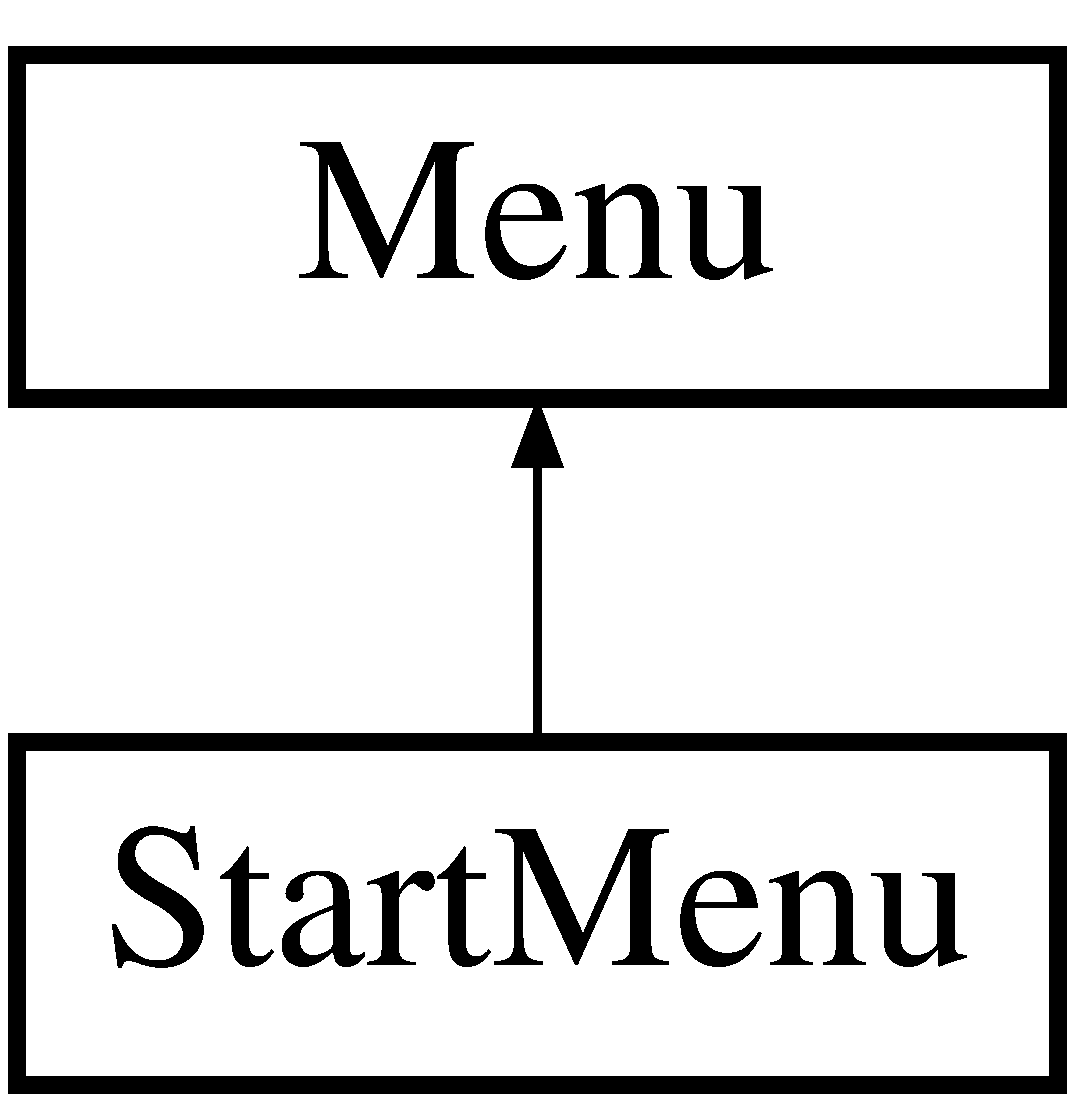
\includegraphics[height=2.000000cm]{class_start_menu}
\end{center}
\end{figure}
\subsection*{Public Member Functions}
\begin{DoxyCompactItemize}
\item 
\hyperlink{class_start_menu_aee52e6dee72aae9ebf1a502f3eaeb4f1}{Start\+Menu} ()
\item 
\hyperlink{class_start_menu_aeb41c71dcfa43b3e9a88c256fc261d99}{Start\+Menu} (std\+::string my\+Texture\+Address, sf\+::\+Vector2u my\+Size, sf\+::\+Vector2i my\+Position)
\item 
\hyperlink{class_start_menu_a0586b30fd5cedbb22ad3a22c98913481}{$\sim$\+Start\+Menu} ()
\item 
void \hyperlink{class_start_menu_a34e56fc211d852a717bef5fc4136d13e}{draw} (sf\+::\+Render\+Window \&)
\item 
void \hyperlink{class_start_menu_a4f6701a9d7a4e08a5212c675ef1c66b2}{resolve\+Event} (sf\+::\+Event)
\item 
void \hyperlink{class_start_menu_a40316866dabe852ee5c931eb5fde164e}{start\+Game} ()
\item 
void \hyperlink{class_start_menu_ab350bdd6779e99bda9f1f4aaa5f02977}{open\+Credits} ()
\item 
void \hyperlink{class_start_menu_a13b4a44809a8c76af1ccfeb97a4d86b5}{exit\+Game} ()
\end{DoxyCompactItemize}
\subsection*{Additional Inherited Members}


\subsection{Constructor \& Destructor Documentation}
\hypertarget{class_start_menu_aee52e6dee72aae9ebf1a502f3eaeb4f1}{\index{Start\+Menu@{Start\+Menu}!Start\+Menu@{Start\+Menu}}
\index{Start\+Menu@{Start\+Menu}!Start\+Menu@{Start\+Menu}}
\subsubsection[{Start\+Menu}]{\setlength{\rightskip}{0pt plus 5cm}Start\+Menu\+::\+Start\+Menu (
\begin{DoxyParamCaption}
{}
\end{DoxyParamCaption}
)}}\label{class_start_menu_aee52e6dee72aae9ebf1a502f3eaeb4f1}
\hypertarget{class_start_menu_aeb41c71dcfa43b3e9a88c256fc261d99}{\index{Start\+Menu@{Start\+Menu}!Start\+Menu@{Start\+Menu}}
\index{Start\+Menu@{Start\+Menu}!Start\+Menu@{Start\+Menu}}
\subsubsection[{Start\+Menu}]{\setlength{\rightskip}{0pt plus 5cm}Start\+Menu\+::\+Start\+Menu (
\begin{DoxyParamCaption}
\item[{std\+::string}]{my\+Texture\+Address, }
\item[{sf\+::\+Vector2u}]{my\+Size, }
\item[{sf\+::\+Vector2i}]{my\+Position}
\end{DoxyParamCaption}
)}}\label{class_start_menu_aeb41c71dcfa43b3e9a88c256fc261d99}
\hypertarget{class_start_menu_a0586b30fd5cedbb22ad3a22c98913481}{\index{Start\+Menu@{Start\+Menu}!````~Start\+Menu@{$\sim$\+Start\+Menu}}
\index{````~Start\+Menu@{$\sim$\+Start\+Menu}!Start\+Menu@{Start\+Menu}}
\subsubsection[{$\sim$\+Start\+Menu}]{\setlength{\rightskip}{0pt plus 5cm}Start\+Menu\+::$\sim$\+Start\+Menu (
\begin{DoxyParamCaption}
{}
\end{DoxyParamCaption}
)}}\label{class_start_menu_a0586b30fd5cedbb22ad3a22c98913481}


\subsection{Member Function Documentation}
\hypertarget{class_start_menu_a34e56fc211d852a717bef5fc4136d13e}{\index{Start\+Menu@{Start\+Menu}!draw@{draw}}
\index{draw@{draw}!Start\+Menu@{Start\+Menu}}
\subsubsection[{draw}]{\setlength{\rightskip}{0pt plus 5cm}void Start\+Menu\+::draw (
\begin{DoxyParamCaption}
\item[{sf\+::\+Render\+Window \&}]{w}
\end{DoxyParamCaption}
)\hspace{0.3cm}{\ttfamily [virtual]}}}\label{class_start_menu_a34e56fc211d852a717bef5fc4136d13e}


Reimplemented from \hyperlink{class_menu_a5c486201ec217b10588c145d043e4eb8}{Menu}.

\hypertarget{class_start_menu_a13b4a44809a8c76af1ccfeb97a4d86b5}{\index{Start\+Menu@{Start\+Menu}!exit\+Game@{exit\+Game}}
\index{exit\+Game@{exit\+Game}!Start\+Menu@{Start\+Menu}}
\subsubsection[{exit\+Game}]{\setlength{\rightskip}{0pt plus 5cm}void Start\+Menu\+::exit\+Game (
\begin{DoxyParamCaption}
{}
\end{DoxyParamCaption}
)}}\label{class_start_menu_a13b4a44809a8c76af1ccfeb97a4d86b5}
\hypertarget{class_start_menu_ab350bdd6779e99bda9f1f4aaa5f02977}{\index{Start\+Menu@{Start\+Menu}!open\+Credits@{open\+Credits}}
\index{open\+Credits@{open\+Credits}!Start\+Menu@{Start\+Menu}}
\subsubsection[{open\+Credits}]{\setlength{\rightskip}{0pt plus 5cm}void Start\+Menu\+::open\+Credits (
\begin{DoxyParamCaption}
{}
\end{DoxyParamCaption}
)}}\label{class_start_menu_ab350bdd6779e99bda9f1f4aaa5f02977}
\hypertarget{class_start_menu_a4f6701a9d7a4e08a5212c675ef1c66b2}{\index{Start\+Menu@{Start\+Menu}!resolve\+Event@{resolve\+Event}}
\index{resolve\+Event@{resolve\+Event}!Start\+Menu@{Start\+Menu}}
\subsubsection[{resolve\+Event}]{\setlength{\rightskip}{0pt plus 5cm}void Start\+Menu\+::resolve\+Event (
\begin{DoxyParamCaption}
\item[{sf\+::\+Event}]{event}
\end{DoxyParamCaption}
)\hspace{0.3cm}{\ttfamily [virtual]}}}\label{class_start_menu_a4f6701a9d7a4e08a5212c675ef1c66b2}


Implements \hyperlink{class_menu_a91ec4d6d898e740524b1fe3312d8f197}{Menu}.

\hypertarget{class_start_menu_a40316866dabe852ee5c931eb5fde164e}{\index{Start\+Menu@{Start\+Menu}!start\+Game@{start\+Game}}
\index{start\+Game@{start\+Game}!Start\+Menu@{Start\+Menu}}
\subsubsection[{start\+Game}]{\setlength{\rightskip}{0pt plus 5cm}void Start\+Menu\+::start\+Game (
\begin{DoxyParamCaption}
{}
\end{DoxyParamCaption}
)}}\label{class_start_menu_a40316866dabe852ee5c931eb5fde164e}


The documentation for this class was generated from the following files\+:\begin{DoxyCompactItemize}
\item 
D\+:/\+Tower\+Defense/\+Tower\+Defense/\hyperlink{_start_menu_8h}{Start\+Menu.\+h}\item 
D\+:/\+Tower\+Defense/\+Tower\+Defense/\hyperlink{_start_menu_8cpp}{Start\+Menu.\+cpp}\end{DoxyCompactItemize}

\hypertarget{class_sun_tower}{\section{Sun\+Tower Class Reference}
\label{class_sun_tower}\index{Sun\+Tower@{Sun\+Tower}}
}


{\ttfamily \#include $<$Sun\+Tower.\+h$>$}

Inheritance diagram for Sun\+Tower\+:\begin{figure}[H]
\begin{center}
\leavevmode
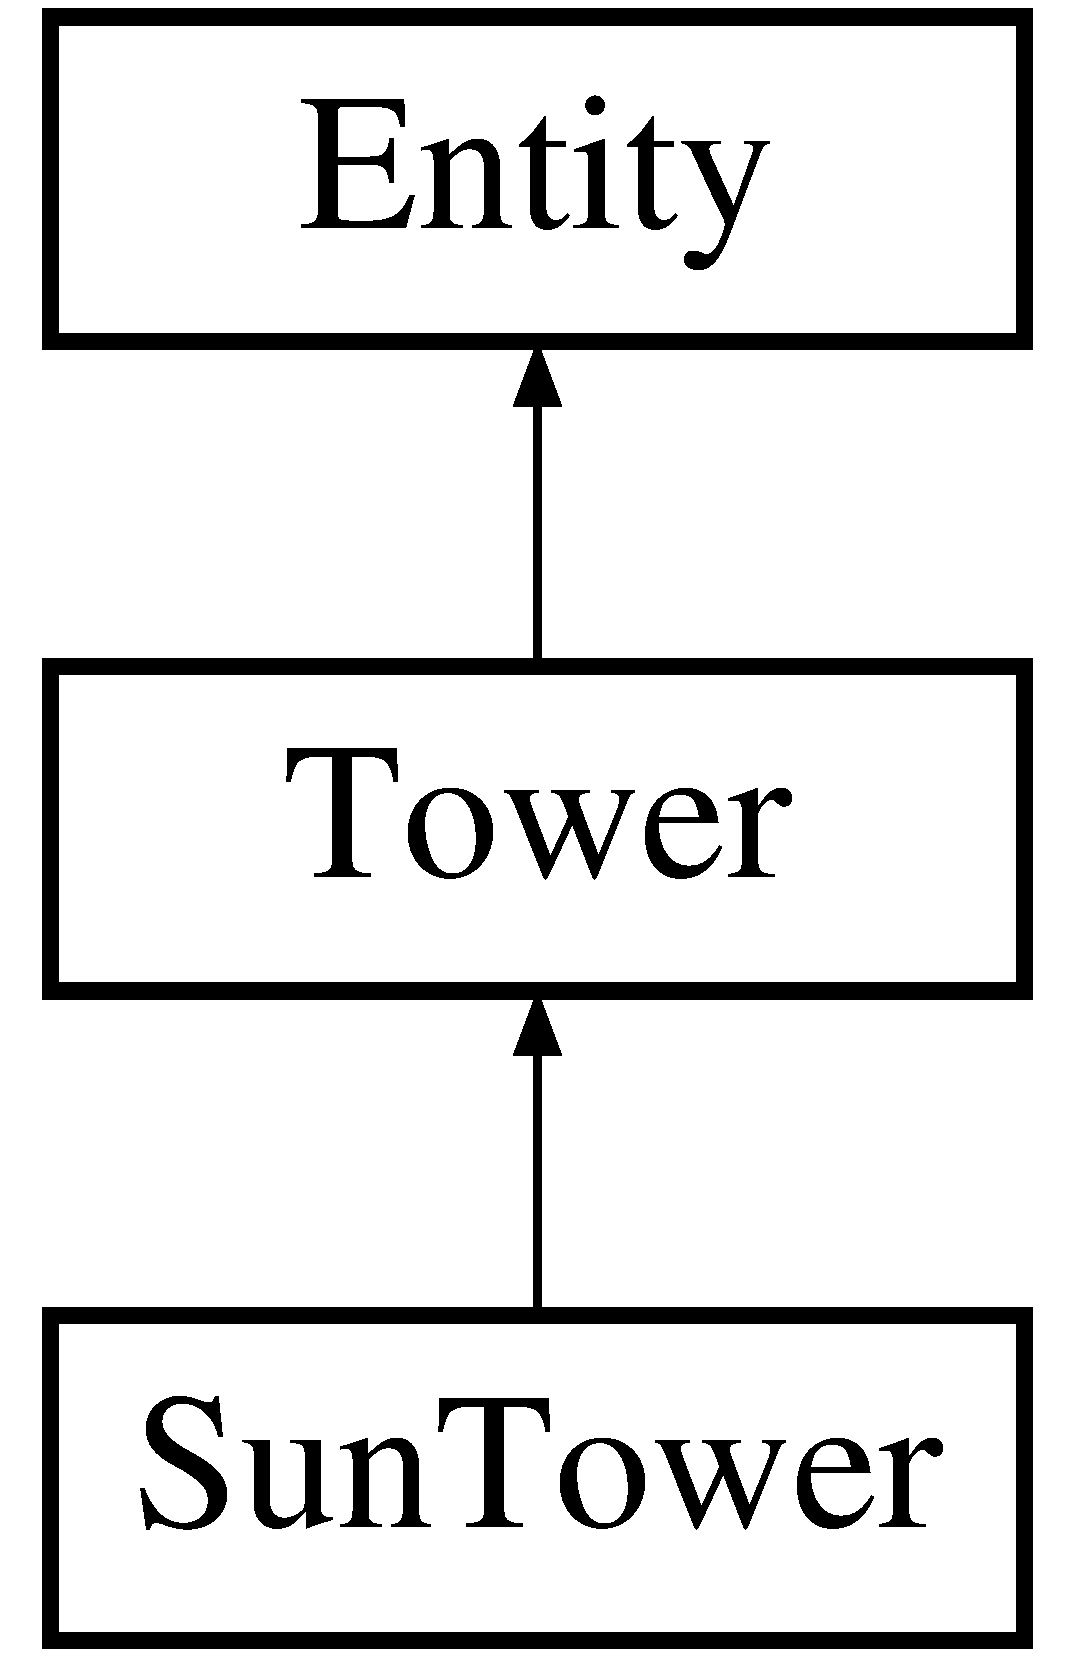
\includegraphics[height=3.000000cm]{class_sun_tower}
\end{center}
\end{figure}
\subsection*{Public Member Functions}
\begin{DoxyCompactItemize}
\item 
\hyperlink{class_sun_tower_aa24e04aa4d64bb77dee9e931b52a3ca5}{Sun\+Tower} (shared\+\_\+ptr$<$ \hyperlink{class_tile}{Tile} $>$ m\+Tile)
\item 
\hyperlink{class_sun_tower_a886c567e4f9c8365336a7c80c2be2af7}{Sun\+Tower} (float m\+Damage, int m\+Price, int m\+Level, float m\+Range, float m\+Speed, sf\+::\+Sprite m\+Sprite)
\item 
virtual \hyperlink{class_sun_tower_ac2ef8bb492fd94f05061eed09ddb900f}{$\sim$\+Sun\+Tower} ()
\item 
void \hyperlink{class_sun_tower_af0453294af7e980271431cab34155cd8}{do\+Attack} (sf\+::\+Render\+Window \&w) override
\end{DoxyCompactItemize}
\subsection*{Additional Inherited Members}


\subsection{Constructor \& Destructor Documentation}
\hypertarget{class_sun_tower_aa24e04aa4d64bb77dee9e931b52a3ca5}{\index{Sun\+Tower@{Sun\+Tower}!Sun\+Tower@{Sun\+Tower}}
\index{Sun\+Tower@{Sun\+Tower}!Sun\+Tower@{Sun\+Tower}}
\subsubsection[{Sun\+Tower}]{\setlength{\rightskip}{0pt plus 5cm}Sun\+Tower\+::\+Sun\+Tower (
\begin{DoxyParamCaption}
\item[{shared\+\_\+ptr$<$ {\bf Tile} $>$}]{m\+Tile}
\end{DoxyParamCaption}
)}}\label{class_sun_tower_aa24e04aa4d64bb77dee9e931b52a3ca5}
\hypertarget{class_sun_tower_a886c567e4f9c8365336a7c80c2be2af7}{\index{Sun\+Tower@{Sun\+Tower}!Sun\+Tower@{Sun\+Tower}}
\index{Sun\+Tower@{Sun\+Tower}!Sun\+Tower@{Sun\+Tower}}
\subsubsection[{Sun\+Tower}]{\setlength{\rightskip}{0pt plus 5cm}Sun\+Tower\+::\+Sun\+Tower (
\begin{DoxyParamCaption}
\item[{float}]{m\+Damage, }
\item[{int}]{m\+Price, }
\item[{int}]{m\+Level, }
\item[{float}]{m\+Range, }
\item[{float}]{m\+Speed, }
\item[{sf\+::\+Sprite}]{m\+Sprite}
\end{DoxyParamCaption}
)}}\label{class_sun_tower_a886c567e4f9c8365336a7c80c2be2af7}
\hypertarget{class_sun_tower_ac2ef8bb492fd94f05061eed09ddb900f}{\index{Sun\+Tower@{Sun\+Tower}!````~Sun\+Tower@{$\sim$\+Sun\+Tower}}
\index{````~Sun\+Tower@{$\sim$\+Sun\+Tower}!Sun\+Tower@{Sun\+Tower}}
\subsubsection[{$\sim$\+Sun\+Tower}]{\setlength{\rightskip}{0pt plus 5cm}virtual Sun\+Tower\+::$\sim$\+Sun\+Tower (
\begin{DoxyParamCaption}
{}
\end{DoxyParamCaption}
)\hspace{0.3cm}{\ttfamily [inline]}, {\ttfamily [virtual]}}}\label{class_sun_tower_ac2ef8bb492fd94f05061eed09ddb900f}


\subsection{Member Function Documentation}
\hypertarget{class_sun_tower_af0453294af7e980271431cab34155cd8}{\index{Sun\+Tower@{Sun\+Tower}!do\+Attack@{do\+Attack}}
\index{do\+Attack@{do\+Attack}!Sun\+Tower@{Sun\+Tower}}
\subsubsection[{do\+Attack}]{\setlength{\rightskip}{0pt plus 5cm}void Sun\+Tower\+::do\+Attack (
\begin{DoxyParamCaption}
\item[{sf\+::\+Render\+Window \&}]{w}
\end{DoxyParamCaption}
)\hspace{0.3cm}{\ttfamily [override]}, {\ttfamily [virtual]}}}\label{class_sun_tower_af0453294af7e980271431cab34155cd8}


Implements \hyperlink{class_tower_a24f01544e308e4b23650779867d54bf8}{Tower}.



The documentation for this class was generated from the following files\+:\begin{DoxyCompactItemize}
\item 
D\+:/\+Tower\+Defense/\+Tower\+Defense/\hyperlink{_sun_tower_8h}{Sun\+Tower.\+h}\item 
D\+:/\+Tower\+Defense/\+Tower\+Defense/\hyperlink{_sun_tower_8cpp}{Sun\+Tower.\+cpp}\end{DoxyCompactItemize}

\hypertarget{class_tile}{\section{Tile Class Reference}
\label{class_tile}\index{Tile@{Tile}}
}


\hyperlink{class_tile}{Tile}.  




{\ttfamily \#include $<$Tile.\+h$>$}

Inheritance diagram for Tile\+:\begin{figure}[H]
\begin{center}
\leavevmode
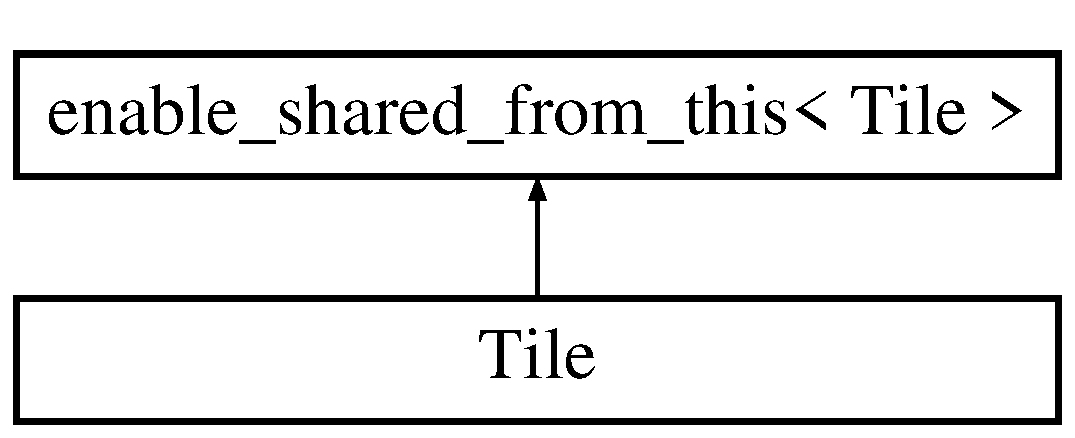
\includegraphics[height=2.000000cm]{class_tile}
\end{center}
\end{figure}
\subsection*{Public Member Functions}
\begin{DoxyCompactItemize}
\item 
\hyperlink{class_tile_aeeb5593bb6b75aae2edfcccbc84ab378}{Tile} ()
\begin{DoxyCompactList}\small\item\em Default constructor. \end{DoxyCompactList}\item 
\hyperlink{class_tile_a837f442dc4576cd22c95fab3bd29dc69}{Tile} (int x, int y)
\begin{DoxyCompactList}\small\item\em Construct the tile with the position of tile. \end{DoxyCompactList}\item 
\hyperlink{class_tile_a98634abbd93fa13d0578d7103202d03d}{$\sim$\+Tile} ()
\begin{DoxyCompactList}\small\item\em Destructor. \end{DoxyCompactList}\item 
sf\+::\+Vector2i \hyperlink{class_tile_ad66322fd7d2cb15d9387a567662c0260}{get\+Position} ()
\begin{DoxyCompactList}\small\item\em Get the position of tile. \end{DoxyCompactList}\item 
sf\+::\+Vector2i \hyperlink{class_tile_adf9367fb8cb9d26f51d692f18ef2d4d3}{get\+Position\+Pixel} ()
\begin{DoxyCompactList}\small\item\em Get the position of the pixel of topleft of the tile. \end{DoxyCompactList}\item 
shared\+\_\+ptr$<$ \hyperlink{class_tower}{Tower} $>$ \hyperlink{class_tile_a741c73bfdb1607240e99f54a6c29153f}{get\+Tower} ()
\begin{DoxyCompactList}\small\item\em Get the pointer of the tower in this tile. \end{DoxyCompactList}\item 
int \hyperlink{class_tile_a49a65d5fb6a4607d21966c82c3198bfb}{get\+Cooldown} ()
\begin{DoxyCompactList}\small\item\em Get the time left for the tower to return normal. \end{DoxyCompactList}\item 
vector$<$ shared\+\_\+ptr$<$ \hyperlink{class_tile}{Tile} $>$ $>$ \hyperlink{class_tile_ad468d33f424d564e0b6c2f0c079ea7ab}{get\+Neighbor} (int range)
\begin{DoxyCompactList}\small\item\em Get all the tiles near this tile. \end{DoxyCompactList}\item 
sf\+::\+Sprite \hyperlink{class_tile_af3dec632de42f9e9784af0dce462837c}{get\+Sprite} ()
\begin{DoxyCompactList}\small\item\em Get the sprite of the tile. \end{DoxyCompactList}\item 
void \hyperlink{class_tile_ad49285b0453a229798c64a08a4480de5}{set\+Position} (sf\+::\+Vector2i pos)
\begin{DoxyCompactList}\small\item\em Set the position of this tile. \end{DoxyCompactList}\item 
void \hyperlink{class_tile_a388c6caf78a0c0063b229c2b10eb4e1c}{set\+Tower} (shared\+\_\+ptr$<$ \hyperlink{class_tower}{Tower} $>$ tower)
\begin{DoxyCompactList}\small\item\em Build a tower in this tile. \end{DoxyCompactList}\item 
void \hyperlink{class_tile_a3976735a9d30faa53e03e72aa08b3a2c}{set\+Cooldown} ()
\begin{DoxyCompactList}\small\item\em Set the time of cooldown for the tower in this tile. \end{DoxyCompactList}\item 
void \hyperlink{class_tile_a597689cfa33df779594c888ee1d0875b}{set\+Sprite} (sf\+::\+Sprite)
\item 
void \hyperlink{class_tile_a0ecef130e42783b84e95408689546f8d}{mouse\+Hover} (sf\+::\+Render\+Window \&w)
\item 
bool \hyperlink{class_tile_ad95f62d8b577df5ace5636a14fb59e6e}{check\+Hover} ()
\item 
bool \hyperlink{class_tile_a802ca0ade47efc9b5f28a047a2f98a96}{check\+Click} ()
\item 
void \hyperlink{class_tile_a398b848f0c6ccfd58245a23e19a7ecc9}{resolve\+Event} (sf\+::\+Event)
\item 
bool \hyperlink{class_tile_a9b3edec9eeb02506164d900e8aecb017}{is\+Polluted} ()
\item 
bool \hyperlink{class_tile_acc84537f5757e5ea52aadcd290ba4f2f}{has\+Tower} ()
\item 
shared\+\_\+ptr$<$ \hyperlink{class_build_menu}{Build\+Menu} $>$ \hyperlink{class_tile_a3192d9456a5ef1ed9e1f6eb447f75cd4}{open\+Build\+Menu} ()
\item 
shared\+\_\+ptr$<$ \hyperlink{class_tower_menu}{Tower\+Menu} $>$ \hyperlink{class_tile_abfe0e5e0a4bd3a5b7194ba7b70e7919e}{open\+Tower\+Menu} ()
\item 
void \hyperlink{class_tile_aa7b74c774f58cc6259a48b144a0a7d14}{draw} (sf\+::\+Render\+Window \&)
\item 
void \hyperlink{class_tile_af11fe597c0bdc2b49d33c4111461ccc4}{sprite\+Update} (int)
\item 
bool \hyperlink{class_tile_ab8081a8e4e47aa339c7ed22ce502afbb}{has\+Enemy} ()
\end{DoxyCompactItemize}


\subsection{Detailed Description}
\hyperlink{class_tile}{Tile}. 

\subsection{Constructor \& Destructor Documentation}
\hypertarget{class_tile_aeeb5593bb6b75aae2edfcccbc84ab378}{\index{Tile@{Tile}!Tile@{Tile}}
\index{Tile@{Tile}!Tile@{Tile}}
\subsubsection[{Tile}]{\setlength{\rightskip}{0pt plus 5cm}Tile\+::\+Tile (
\begin{DoxyParamCaption}
{}
\end{DoxyParamCaption}
)}}\label{class_tile_aeeb5593bb6b75aae2edfcccbc84ab378}


Default constructor. 

\hypertarget{class_tile_a837f442dc4576cd22c95fab3bd29dc69}{\index{Tile@{Tile}!Tile@{Tile}}
\index{Tile@{Tile}!Tile@{Tile}}
\subsubsection[{Tile}]{\setlength{\rightskip}{0pt plus 5cm}Tile\+::\+Tile (
\begin{DoxyParamCaption}
\item[{int}]{x, }
\item[{int}]{y}
\end{DoxyParamCaption}
)}}\label{class_tile_a837f442dc4576cd22c95fab3bd29dc69}


Construct the tile with the position of tile. 


\begin{DoxyParams}{Parameters}
{\em x} & the row of the tile. \\
\hline
{\em y} & the collone of the tile. \\
\hline
\end{DoxyParams}
\hypertarget{class_tile_a98634abbd93fa13d0578d7103202d03d}{\index{Tile@{Tile}!````~Tile@{$\sim$\+Tile}}
\index{````~Tile@{$\sim$\+Tile}!Tile@{Tile}}
\subsubsection[{$\sim$\+Tile}]{\setlength{\rightskip}{0pt plus 5cm}Tile\+::$\sim$\+Tile (
\begin{DoxyParamCaption}
{}
\end{DoxyParamCaption}
)}}\label{class_tile_a98634abbd93fa13d0578d7103202d03d}


Destructor. 



\subsection{Member Function Documentation}
\hypertarget{class_tile_a802ca0ade47efc9b5f28a047a2f98a96}{\index{Tile@{Tile}!check\+Click@{check\+Click}}
\index{check\+Click@{check\+Click}!Tile@{Tile}}
\subsubsection[{check\+Click}]{\setlength{\rightskip}{0pt plus 5cm}bool Tile\+::check\+Click (
\begin{DoxyParamCaption}
{}
\end{DoxyParamCaption}
)}}\label{class_tile_a802ca0ade47efc9b5f28a047a2f98a96}
\hypertarget{class_tile_ad95f62d8b577df5ace5636a14fb59e6e}{\index{Tile@{Tile}!check\+Hover@{check\+Hover}}
\index{check\+Hover@{check\+Hover}!Tile@{Tile}}
\subsubsection[{check\+Hover}]{\setlength{\rightskip}{0pt plus 5cm}bool Tile\+::check\+Hover (
\begin{DoxyParamCaption}
{}
\end{DoxyParamCaption}
)}}\label{class_tile_ad95f62d8b577df5ace5636a14fb59e6e}
\hypertarget{class_tile_aa7b74c774f58cc6259a48b144a0a7d14}{\index{Tile@{Tile}!draw@{draw}}
\index{draw@{draw}!Tile@{Tile}}
\subsubsection[{draw}]{\setlength{\rightskip}{0pt plus 5cm}void Tile\+::draw (
\begin{DoxyParamCaption}
\item[{sf\+::\+Render\+Window \&}]{w}
\end{DoxyParamCaption}
)}}\label{class_tile_aa7b74c774f58cc6259a48b144a0a7d14}
\hypertarget{class_tile_a49a65d5fb6a4607d21966c82c3198bfb}{\index{Tile@{Tile}!get\+Cooldown@{get\+Cooldown}}
\index{get\+Cooldown@{get\+Cooldown}!Tile@{Tile}}
\subsubsection[{get\+Cooldown}]{\setlength{\rightskip}{0pt plus 5cm}int Tile\+::get\+Cooldown (
\begin{DoxyParamCaption}
{}
\end{DoxyParamCaption}
)}}\label{class_tile_a49a65d5fb6a4607d21966c82c3198bfb}


Get the time left for the tower to return normal. 

\begin{DoxyReturn}{Returns}
An integer which means the time left for the tile to become nomal. 
\end{DoxyReturn}
\hypertarget{class_tile_ad468d33f424d564e0b6c2f0c079ea7ab}{\index{Tile@{Tile}!get\+Neighbor@{get\+Neighbor}}
\index{get\+Neighbor@{get\+Neighbor}!Tile@{Tile}}
\subsubsection[{get\+Neighbor}]{\setlength{\rightskip}{0pt plus 5cm}std\+::vector$<$ shared\+\_\+ptr$<$ {\bf Tile} $>$ $>$ Tile\+::get\+Neighbor (
\begin{DoxyParamCaption}
\item[{int}]{range}
\end{DoxyParamCaption}
)}}\label{class_tile_ad468d33f424d564e0b6c2f0c079ea7ab}


Get all the tiles near this tile. 


\begin{DoxyParams}{Parameters}
{\em range} & is the distance entre two tiles. It can be 1, 2, 3. \\
\hline
\end{DoxyParams}
\begin{DoxyReturn}{Returns}
A vactor contains all the shared pointers of the tile near this tile. 
\end{DoxyReturn}
\hypertarget{class_tile_ad66322fd7d2cb15d9387a567662c0260}{\index{Tile@{Tile}!get\+Position@{get\+Position}}
\index{get\+Position@{get\+Position}!Tile@{Tile}}
\subsubsection[{get\+Position}]{\setlength{\rightskip}{0pt plus 5cm}sf\+::\+Vector2i Tile\+::get\+Position (
\begin{DoxyParamCaption}
{}
\end{DoxyParamCaption}
)}}\label{class_tile_ad66322fd7d2cb15d9387a567662c0260}


Get the position of tile. 

\begin{DoxyReturn}{Returns}
The position in forme sf\+::\+Vector2i.(x,y) is row and collone of the tile. 
\end{DoxyReturn}
\hypertarget{class_tile_adf9367fb8cb9d26f51d692f18ef2d4d3}{\index{Tile@{Tile}!get\+Position\+Pixel@{get\+Position\+Pixel}}
\index{get\+Position\+Pixel@{get\+Position\+Pixel}!Tile@{Tile}}
\subsubsection[{get\+Position\+Pixel}]{\setlength{\rightskip}{0pt plus 5cm}sf\+::\+Vector2i Tile\+::get\+Position\+Pixel (
\begin{DoxyParamCaption}
{}
\end{DoxyParamCaption}
)}}\label{class_tile_adf9367fb8cb9d26f51d692f18ef2d4d3}


Get the position of the pixel of topleft of the tile. 

\begin{DoxyReturn}{Returns}
The position in forme sf\+::\+Vector2i. 
\end{DoxyReturn}
\hypertarget{class_tile_af3dec632de42f9e9784af0dce462837c}{\index{Tile@{Tile}!get\+Sprite@{get\+Sprite}}
\index{get\+Sprite@{get\+Sprite}!Tile@{Tile}}
\subsubsection[{get\+Sprite}]{\setlength{\rightskip}{0pt plus 5cm}sf\+::\+Sprite Tile\+::get\+Sprite (
\begin{DoxyParamCaption}
{}
\end{DoxyParamCaption}
)}}\label{class_tile_af3dec632de42f9e9784af0dce462837c}


Get the sprite of the tile. 

\begin{DoxyReturn}{Returns}
The sprite. 
\end{DoxyReturn}
\hypertarget{class_tile_a741c73bfdb1607240e99f54a6c29153f}{\index{Tile@{Tile}!get\+Tower@{get\+Tower}}
\index{get\+Tower@{get\+Tower}!Tile@{Tile}}
\subsubsection[{get\+Tower}]{\setlength{\rightskip}{0pt plus 5cm}shared\+\_\+ptr$<$ {\bf Tower} $>$ Tile\+::get\+Tower (
\begin{DoxyParamCaption}
{}
\end{DoxyParamCaption}
)}}\label{class_tile_a741c73bfdb1607240e99f54a6c29153f}


Get the pointer of the tower in this tile. 

\begin{DoxyReturn}{Returns}
A shared pointer of the tower in this tile. 
\end{DoxyReturn}
\hypertarget{class_tile_ab8081a8e4e47aa339c7ed22ce502afbb}{\index{Tile@{Tile}!has\+Enemy@{has\+Enemy}}
\index{has\+Enemy@{has\+Enemy}!Tile@{Tile}}
\subsubsection[{has\+Enemy}]{\setlength{\rightskip}{0pt plus 5cm}bool Tile\+::has\+Enemy (
\begin{DoxyParamCaption}
{}
\end{DoxyParamCaption}
)}}\label{class_tile_ab8081a8e4e47aa339c7ed22ce502afbb}
\hypertarget{class_tile_acc84537f5757e5ea52aadcd290ba4f2f}{\index{Tile@{Tile}!has\+Tower@{has\+Tower}}
\index{has\+Tower@{has\+Tower}!Tile@{Tile}}
\subsubsection[{has\+Tower}]{\setlength{\rightskip}{0pt plus 5cm}bool Tile\+::has\+Tower (
\begin{DoxyParamCaption}
{}
\end{DoxyParamCaption}
)}}\label{class_tile_acc84537f5757e5ea52aadcd290ba4f2f}
\hypertarget{class_tile_a9b3edec9eeb02506164d900e8aecb017}{\index{Tile@{Tile}!is\+Polluted@{is\+Polluted}}
\index{is\+Polluted@{is\+Polluted}!Tile@{Tile}}
\subsubsection[{is\+Polluted}]{\setlength{\rightskip}{0pt plus 5cm}bool Tile\+::is\+Polluted (
\begin{DoxyParamCaption}
{}
\end{DoxyParamCaption}
)}}\label{class_tile_a9b3edec9eeb02506164d900e8aecb017}
\hypertarget{class_tile_a0ecef130e42783b84e95408689546f8d}{\index{Tile@{Tile}!mouse\+Hover@{mouse\+Hover}}
\index{mouse\+Hover@{mouse\+Hover}!Tile@{Tile}}
\subsubsection[{mouse\+Hover}]{\setlength{\rightskip}{0pt plus 5cm}void Tile\+::mouse\+Hover (
\begin{DoxyParamCaption}
\item[{sf\+::\+Render\+Window \&}]{w}
\end{DoxyParamCaption}
)}}\label{class_tile_a0ecef130e42783b84e95408689546f8d}
\hypertarget{class_tile_a3192d9456a5ef1ed9e1f6eb447f75cd4}{\index{Tile@{Tile}!open\+Build\+Menu@{open\+Build\+Menu}}
\index{open\+Build\+Menu@{open\+Build\+Menu}!Tile@{Tile}}
\subsubsection[{open\+Build\+Menu}]{\setlength{\rightskip}{0pt plus 5cm}shared\+\_\+ptr$<$ {\bf Build\+Menu} $>$ Tile\+::open\+Build\+Menu (
\begin{DoxyParamCaption}
{}
\end{DoxyParamCaption}
)}}\label{class_tile_a3192d9456a5ef1ed9e1f6eb447f75cd4}
\hypertarget{class_tile_abfe0e5e0a4bd3a5b7194ba7b70e7919e}{\index{Tile@{Tile}!open\+Tower\+Menu@{open\+Tower\+Menu}}
\index{open\+Tower\+Menu@{open\+Tower\+Menu}!Tile@{Tile}}
\subsubsection[{open\+Tower\+Menu}]{\setlength{\rightskip}{0pt plus 5cm}shared\+\_\+ptr$<$ {\bf Tower\+Menu} $>$ Tile\+::open\+Tower\+Menu (
\begin{DoxyParamCaption}
{}
\end{DoxyParamCaption}
)}}\label{class_tile_abfe0e5e0a4bd3a5b7194ba7b70e7919e}
\hypertarget{class_tile_a398b848f0c6ccfd58245a23e19a7ecc9}{\index{Tile@{Tile}!resolve\+Event@{resolve\+Event}}
\index{resolve\+Event@{resolve\+Event}!Tile@{Tile}}
\subsubsection[{resolve\+Event}]{\setlength{\rightskip}{0pt plus 5cm}void Tile\+::resolve\+Event (
\begin{DoxyParamCaption}
\item[{sf\+::\+Event}]{event}
\end{DoxyParamCaption}
)}}\label{class_tile_a398b848f0c6ccfd58245a23e19a7ecc9}
\hypertarget{class_tile_a3976735a9d30faa53e03e72aa08b3a2c}{\index{Tile@{Tile}!set\+Cooldown@{set\+Cooldown}}
\index{set\+Cooldown@{set\+Cooldown}!Tile@{Tile}}
\subsubsection[{set\+Cooldown}]{\setlength{\rightskip}{0pt plus 5cm}void Tile\+::set\+Cooldown (
\begin{DoxyParamCaption}
{}
\end{DoxyParamCaption}
)}}\label{class_tile_a3976735a9d30faa53e03e72aa08b3a2c}


Set the time of cooldown for the tower in this tile. 

Set the time \hypertarget{class_tile_ad49285b0453a229798c64a08a4480de5}{\index{Tile@{Tile}!set\+Position@{set\+Position}}
\index{set\+Position@{set\+Position}!Tile@{Tile}}
\subsubsection[{set\+Position}]{\setlength{\rightskip}{0pt plus 5cm}void Tile\+::set\+Position (
\begin{DoxyParamCaption}
\item[{sf\+::\+Vector2i}]{pos}
\end{DoxyParamCaption}
)}}\label{class_tile_ad49285b0453a229798c64a08a4480de5}


Set the position of this tile. 


\begin{DoxyParams}{Parameters}
{\em pos} & is the postion that will be set to the tile. \\
\hline
\end{DoxyParams}
\hypertarget{class_tile_a597689cfa33df779594c888ee1d0875b}{\index{Tile@{Tile}!set\+Sprite@{set\+Sprite}}
\index{set\+Sprite@{set\+Sprite}!Tile@{Tile}}
\subsubsection[{set\+Sprite}]{\setlength{\rightskip}{0pt plus 5cm}void Tile\+::set\+Sprite (
\begin{DoxyParamCaption}
\item[{sf\+::\+Sprite}]{my\+Sprite}
\end{DoxyParamCaption}
)}}\label{class_tile_a597689cfa33df779594c888ee1d0875b}
\hypertarget{class_tile_a388c6caf78a0c0063b229c2b10eb4e1c}{\index{Tile@{Tile}!set\+Tower@{set\+Tower}}
\index{set\+Tower@{set\+Tower}!Tile@{Tile}}
\subsubsection[{set\+Tower}]{\setlength{\rightskip}{0pt plus 5cm}void Tile\+::set\+Tower (
\begin{DoxyParamCaption}
\item[{shared\+\_\+ptr$<$ {\bf Tower} $>$}]{tower}
\end{DoxyParamCaption}
)}}\label{class_tile_a388c6caf78a0c0063b229c2b10eb4e1c}


Build a tower in this tile. 


\begin{DoxyParams}{Parameters}
{\em tower} & is the tower built in this tile. \\
\hline
\end{DoxyParams}
\hypertarget{class_tile_af11fe597c0bdc2b49d33c4111461ccc4}{\index{Tile@{Tile}!sprite\+Update@{sprite\+Update}}
\index{sprite\+Update@{sprite\+Update}!Tile@{Tile}}
\subsubsection[{sprite\+Update}]{\setlength{\rightskip}{0pt plus 5cm}void Tile\+::sprite\+Update (
\begin{DoxyParamCaption}
\item[{int}]{i}
\end{DoxyParamCaption}
)}}\label{class_tile_af11fe597c0bdc2b49d33c4111461ccc4}


The documentation for this class was generated from the following files\+:\begin{DoxyCompactItemize}
\item 
D\+:/\+Tower\+Defense/\+Tower\+Defense/\hyperlink{_tile_8h}{Tile.\+h}\item 
D\+:/\+Tower\+Defense/\+Tower\+Defense/\hyperlink{_tile_8cpp}{Tile.\+cpp}\end{DoxyCompactItemize}

\hypertarget{class_tough_enemy}{\section{Tough\+Enemy Class Reference}
\label{class_tough_enemy}\index{Tough\+Enemy@{Tough\+Enemy}}
}


{\ttfamily \#include $<$Tough\+Enemy.\+h$>$}

Inheritance diagram for Tough\+Enemy\+:\begin{figure}[H]
\begin{center}
\leavevmode
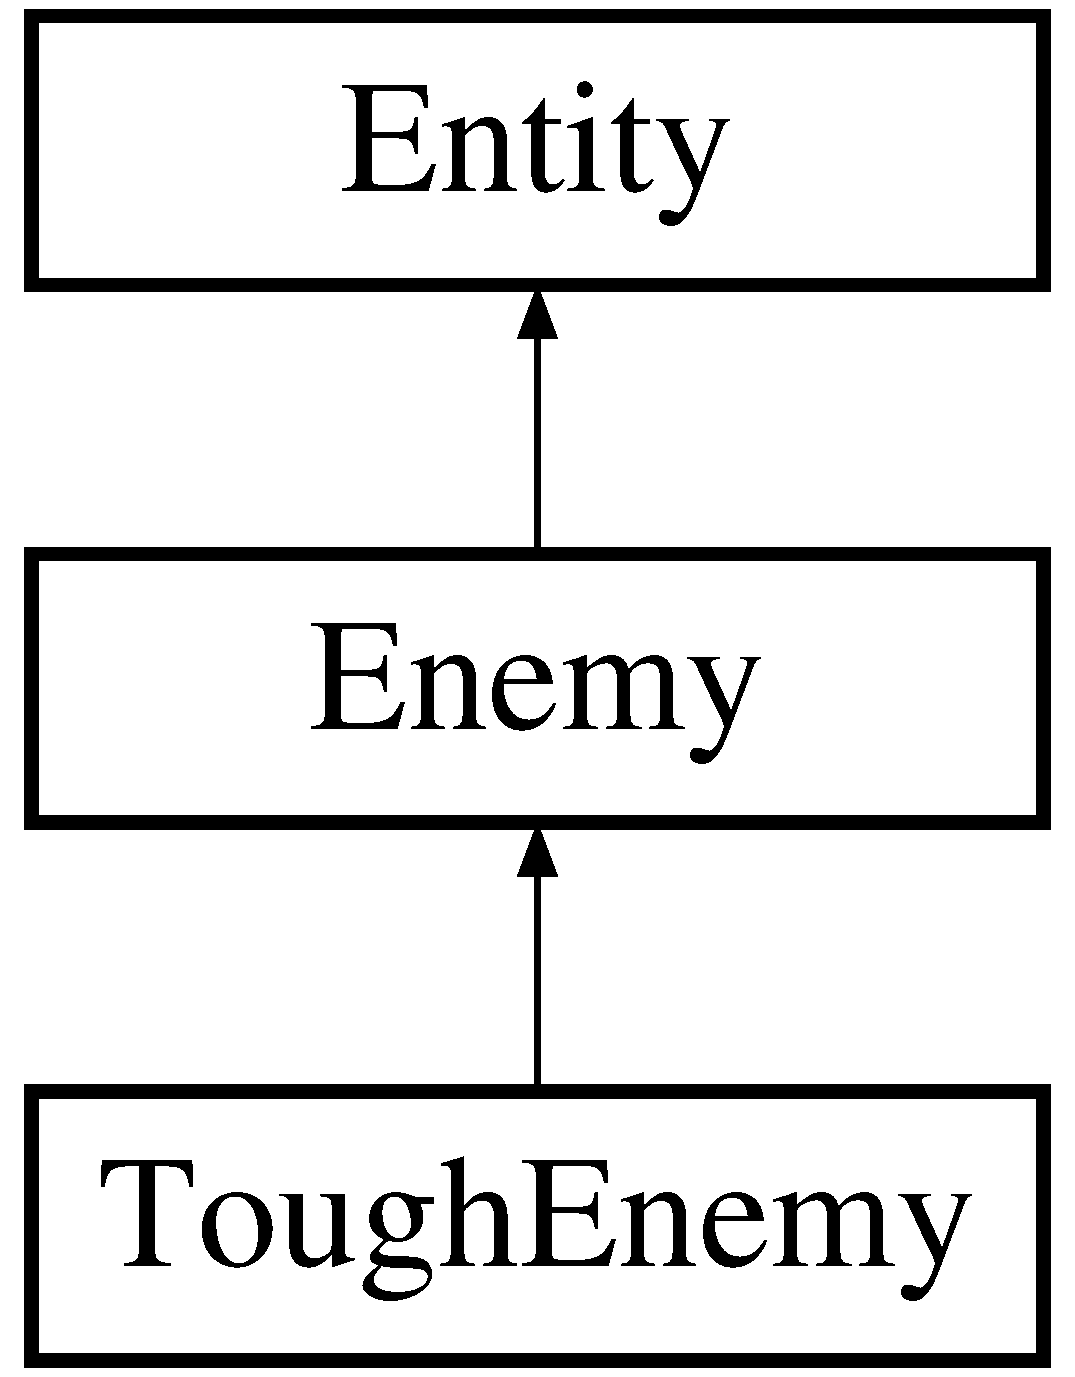
\includegraphics[height=3.000000cm]{class_tough_enemy}
\end{center}
\end{figure}
\subsection*{Public Member Functions}
\begin{DoxyCompactItemize}
\item 
\hyperlink{class_tough_enemy_aceaf7ef1a1ec0d4eda307b0b9b2d89da}{Tough\+Enemy} ()
\item 
\hyperlink{class_tough_enemy_a2de3dde139f0a1f11e3e1bf0540d11d9}{Tough\+Enemy} (int \hyperlink{class_enemy_a278d70100af07c946743db1b7a1a9f59}{hp}, float \hyperlink{class_enemy_a9bb5d74024760e604c41ba79cc7da892}{defence}, int \hyperlink{class_enemy_a1d9a86d110b87f3cc55b40d1bdb59eb5}{bounty}, int \hyperlink{class_enemy_abc49d5a2cef917c8ece8a16547f8efee}{score\+Value}, sf\+::\+Sprite \hyperlink{class_entity_a48ef4ab143b8d0211877c9f6be42e824}{sprite}, float \hyperlink{class_entity_a1de3d8d9ab8088f61e6726069b26fa60}{speed})
\item 
virtual \hyperlink{class_tough_enemy_ae99335f00c32922c352c476c764f99d1}{$\sim$\+Tough\+Enemy} ()
\item 
string \hyperlink{class_tough_enemy_aec2e1a119c04896b1bd5aa7b36e2acca}{test} ()
\end{DoxyCompactItemize}
\subsection*{Additional Inherited Members}


\subsection{Constructor \& Destructor Documentation}
\hypertarget{class_tough_enemy_aceaf7ef1a1ec0d4eda307b0b9b2d89da}{\index{Tough\+Enemy@{Tough\+Enemy}!Tough\+Enemy@{Tough\+Enemy}}
\index{Tough\+Enemy@{Tough\+Enemy}!Tough\+Enemy@{Tough\+Enemy}}
\subsubsection[{Tough\+Enemy}]{\setlength{\rightskip}{0pt plus 5cm}Tough\+Enemy\+::\+Tough\+Enemy (
\begin{DoxyParamCaption}
{}
\end{DoxyParamCaption}
)}}\label{class_tough_enemy_aceaf7ef1a1ec0d4eda307b0b9b2d89da}
\hypertarget{class_tough_enemy_a2de3dde139f0a1f11e3e1bf0540d11d9}{\index{Tough\+Enemy@{Tough\+Enemy}!Tough\+Enemy@{Tough\+Enemy}}
\index{Tough\+Enemy@{Tough\+Enemy}!Tough\+Enemy@{Tough\+Enemy}}
\subsubsection[{Tough\+Enemy}]{\setlength{\rightskip}{0pt plus 5cm}Tough\+Enemy\+::\+Tough\+Enemy (
\begin{DoxyParamCaption}
\item[{int}]{hp, }
\item[{float}]{defence, }
\item[{int}]{bounty, }
\item[{int}]{score\+Value, }
\item[{sf\+::\+Sprite}]{sprite, }
\item[{float}]{speed}
\end{DoxyParamCaption}
)}}\label{class_tough_enemy_a2de3dde139f0a1f11e3e1bf0540d11d9}
\hypertarget{class_tough_enemy_ae99335f00c32922c352c476c764f99d1}{\index{Tough\+Enemy@{Tough\+Enemy}!````~Tough\+Enemy@{$\sim$\+Tough\+Enemy}}
\index{````~Tough\+Enemy@{$\sim$\+Tough\+Enemy}!Tough\+Enemy@{Tough\+Enemy}}
\subsubsection[{$\sim$\+Tough\+Enemy}]{\setlength{\rightskip}{0pt plus 5cm}virtual Tough\+Enemy\+::$\sim$\+Tough\+Enemy (
\begin{DoxyParamCaption}
{}
\end{DoxyParamCaption}
)\hspace{0.3cm}{\ttfamily [inline]}, {\ttfamily [virtual]}}}\label{class_tough_enemy_ae99335f00c32922c352c476c764f99d1}


\subsection{Member Function Documentation}
\hypertarget{class_tough_enemy_aec2e1a119c04896b1bd5aa7b36e2acca}{\index{Tough\+Enemy@{Tough\+Enemy}!test@{test}}
\index{test@{test}!Tough\+Enemy@{Tough\+Enemy}}
\subsubsection[{test}]{\setlength{\rightskip}{0pt plus 5cm}string Tough\+Enemy\+::test (
\begin{DoxyParamCaption}
{}
\end{DoxyParamCaption}
)\hspace{0.3cm}{\ttfamily [inline]}, {\ttfamily [virtual]}}}\label{class_tough_enemy_aec2e1a119c04896b1bd5aa7b36e2acca}


Implements \hyperlink{class_enemy_a37b2bae4f5a9e8d673aeb28880ded0bc}{Enemy}.



The documentation for this class was generated from the following files\+:\begin{DoxyCompactItemize}
\item 
D\+:/\+Tower\+Defense/\+Tower\+Defense/\hyperlink{_tough_enemy_8h}{Tough\+Enemy.\+h}\item 
D\+:/\+Tower\+Defense/\+Tower\+Defense/\hyperlink{_tough_enemy_8cpp}{Tough\+Enemy.\+cpp}\end{DoxyCompactItemize}

\hypertarget{class_tower}{\section{Tower Class Reference}
\label{class_tower}\index{Tower@{Tower}}
}


{\ttfamily \#include $<$Tower.\+h$>$}

Inheritance diagram for Tower\+:\begin{figure}[H]
\begin{center}
\leavevmode
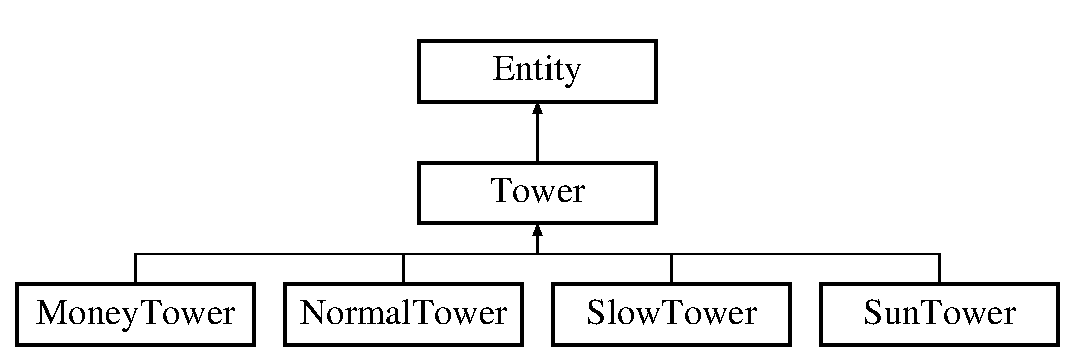
\includegraphics[height=3.000000cm]{class_tower}
\end{center}
\end{figure}
\subsection*{Public Member Functions}
\begin{DoxyCompactItemize}
\item 
\hyperlink{class_tower_a2fd91cfd06bdbb8c5e26b3d5e30770d8}{Tower} (shared\+\_\+ptr$<$ \hyperlink{class_tile}{Tile} $>$)
\item 
\hyperlink{class_tower_a1b785dc1e9fb979a10620ca183b5761d}{Tower} ()
\item 
virtual \hyperlink{class_tower_a96972da33c287758c036c944eccdc5fe}{$\sim$\+Tower} ()
\item 
float \hyperlink{class_tower_acdcf79c9b6c65a9e5134ec249bf6bd4a}{get\+Damage} ()
\item 
int \hyperlink{class_tower_a3b495235e7ca4a76c858d62ba1775aac}{get\+Price} ()
\item 
int \hyperlink{class_tower_ad1fe459e4a6e4a8a6976001ea53a06a7}{get\+Level} ()
\item 
float \hyperlink{class_tower_abbb4fe2239e90f18095e79680dbfd63c}{get\+Range} ()
\item 
int \hyperlink{class_tower_ad8049d4e63bd6b86e962d022df7d05d1}{get\+Income} ()
\item 
void \hyperlink{class_tower_adb91589e341ed1408649ed2310da301b}{set\+Damage} (float m\+Damage)
\item 
void \hyperlink{class_tower_a3ebb2953cea4fb88b0d7f50124f022c2}{set\+Price} (int m\+Price)
\item 
void \hyperlink{class_tower_aa6325131f3ea5cef244cd6b50e770325}{set\+Level} (int m\+Level)
\item 
void \hyperlink{class_tower_a776ebeb91a1d5060ac415fedb0dda0ce}{set\+Range} (float m\+Range)
\item 
void \hyperlink{class_tower_ad9707bfc7619402f7899e7dfe3246f76}{set\+Attack} ()
\item 
void \hyperlink{class_tower_a4f3edbbfcd0908c398057d2608ca88d9}{set\+Tower\+Texture} ()
\item 
void \hyperlink{class_tower_a46b76511c60eff0e0c0b094bd0a16d34}{set\+Range\+Circle} ()
\item 
void \hyperlink{class_tower_a745854abfacb9b27ae1c0b8863713283}{sell\+Tw} ()
\item 
void \hyperlink{class_tower_a34ffa45b1ad095499df291fc5b7c8083}{upgrade\+Tw} ()
\item 
void \hyperlink{class_tower_a72a405119bb68e7169a688e987aeaa70}{downgrade\+Tw} ()
\item 
virtual void \hyperlink{class_tower_a24f01544e308e4b23650779867d54bf8}{do\+Attack} (sf\+::\+Render\+Window \&w)=0
\item 
void \hyperlink{class_tower_af1ab9b841310f9cfb929311c20feb337}{sprite\+Update} (int i)
\item 
void \hyperlink{class_tower_a830f388d79414d79f0eb141f53515c49}{show\+Range\+Circle} (sf\+::\+Render\+Window \&w)
\end{DoxyCompactItemize}
\subsection*{Protected Attributes}
\begin{DoxyCompactItemize}
\item 
shared\+\_\+ptr$<$ \hyperlink{class_attack}{Attack} $>$ \hyperlink{class_tower_a4269c70ee90c69a064bc6d6690bb354a}{attack}
\item 
float \hyperlink{class_tower_a6486b52fd99b92955a2f3424884286b9}{damage} \mbox{[}3\mbox{]}
\item 
int \hyperlink{class_tower_a88bb2c4d038523ab9430d69ffe508cf1}{slow\+Amount} \mbox{[}3\mbox{]}
\item 
float \hyperlink{class_tower_a7e59dee11464af7439163088ac988955}{range} \mbox{[}3\mbox{]}
\item 
int \hyperlink{class_tower_a06784c625069968923cf19a0cecdf37e}{speed} \mbox{[}3\mbox{]}
\item 
int \hyperlink{class_tower_a9e86386041605d8b9f53356c6fc18d34}{income} \mbox{[}3\mbox{]}
\item 
int \hyperlink{class_tower_afb26e285e0177b99871e7ad2b603a459}{price}
\item 
int \hyperlink{class_tower_a586375a39e6817983339b36225379da0}{level}
\item 
int \hyperlink{class_tower_ae9ab0c86f3c1bdd5e73a5cdee4bdfd96}{current\+Sprite}
\item 
sf\+::\+Circle\+Shape \hyperlink{class_tower_a4b4dd0d7a6a3469de2e93421156a6486}{range\+Circle}
\end{DoxyCompactItemize}


\subsection{Constructor \& Destructor Documentation}
\hypertarget{class_tower_a2fd91cfd06bdbb8c5e26b3d5e30770d8}{\index{Tower@{Tower}!Tower@{Tower}}
\index{Tower@{Tower}!Tower@{Tower}}
\subsubsection[{Tower}]{\setlength{\rightskip}{0pt plus 5cm}Tower\+::\+Tower (
\begin{DoxyParamCaption}
\item[{shared\+\_\+ptr$<$ {\bf Tile} $>$}]{m\+Tile}
\end{DoxyParamCaption}
)}}\label{class_tower_a2fd91cfd06bdbb8c5e26b3d5e30770d8}
\hypertarget{class_tower_a1b785dc1e9fb979a10620ca183b5761d}{\index{Tower@{Tower}!Tower@{Tower}}
\index{Tower@{Tower}!Tower@{Tower}}
\subsubsection[{Tower}]{\setlength{\rightskip}{0pt plus 5cm}Tower\+::\+Tower (
\begin{DoxyParamCaption}
{}
\end{DoxyParamCaption}
)}}\label{class_tower_a1b785dc1e9fb979a10620ca183b5761d}
\hypertarget{class_tower_a96972da33c287758c036c944eccdc5fe}{\index{Tower@{Tower}!````~Tower@{$\sim$\+Tower}}
\index{````~Tower@{$\sim$\+Tower}!Tower@{Tower}}
\subsubsection[{$\sim$\+Tower}]{\setlength{\rightskip}{0pt plus 5cm}Tower\+::$\sim$\+Tower (
\begin{DoxyParamCaption}
{}
\end{DoxyParamCaption}
)\hspace{0.3cm}{\ttfamily [virtual]}}}\label{class_tower_a96972da33c287758c036c944eccdc5fe}


\subsection{Member Function Documentation}
\hypertarget{class_tower_a24f01544e308e4b23650779867d54bf8}{\index{Tower@{Tower}!do\+Attack@{do\+Attack}}
\index{do\+Attack@{do\+Attack}!Tower@{Tower}}
\subsubsection[{do\+Attack}]{\setlength{\rightskip}{0pt plus 5cm}virtual void Tower\+::do\+Attack (
\begin{DoxyParamCaption}
\item[{sf\+::\+Render\+Window \&}]{w}
\end{DoxyParamCaption}
)\hspace{0.3cm}{\ttfamily [pure virtual]}}}\label{class_tower_a24f01544e308e4b23650779867d54bf8}


Implemented in \hyperlink{class_money_tower_a83e66451e2e45ab85ffc2fa69ae79192}{Money\+Tower}, \hyperlink{class_normal_tower_a1e3b0a2216d943650b060bac297511b6}{Normal\+Tower}, \hyperlink{class_slow_tower_a263531cb94fccecfdc1bd667a54b168d}{Slow\+Tower}, and \hyperlink{class_sun_tower_af0453294af7e980271431cab34155cd8}{Sun\+Tower}.

\hypertarget{class_tower_a72a405119bb68e7169a688e987aeaa70}{\index{Tower@{Tower}!downgrade\+Tw@{downgrade\+Tw}}
\index{downgrade\+Tw@{downgrade\+Tw}!Tower@{Tower}}
\subsubsection[{downgrade\+Tw}]{\setlength{\rightskip}{0pt plus 5cm}void Tower\+::downgrade\+Tw (
\begin{DoxyParamCaption}
{}
\end{DoxyParamCaption}
)}}\label{class_tower_a72a405119bb68e7169a688e987aeaa70}
\hypertarget{class_tower_acdcf79c9b6c65a9e5134ec249bf6bd4a}{\index{Tower@{Tower}!get\+Damage@{get\+Damage}}
\index{get\+Damage@{get\+Damage}!Tower@{Tower}}
\subsubsection[{get\+Damage}]{\setlength{\rightskip}{0pt plus 5cm}float Tower\+::get\+Damage (
\begin{DoxyParamCaption}
{}
\end{DoxyParamCaption}
)}}\label{class_tower_acdcf79c9b6c65a9e5134ec249bf6bd4a}
\hypertarget{class_tower_ad8049d4e63bd6b86e962d022df7d05d1}{\index{Tower@{Tower}!get\+Income@{get\+Income}}
\index{get\+Income@{get\+Income}!Tower@{Tower}}
\subsubsection[{get\+Income}]{\setlength{\rightskip}{0pt plus 5cm}int Tower\+::get\+Income (
\begin{DoxyParamCaption}
{}
\end{DoxyParamCaption}
)}}\label{class_tower_ad8049d4e63bd6b86e962d022df7d05d1}
\hypertarget{class_tower_ad1fe459e4a6e4a8a6976001ea53a06a7}{\index{Tower@{Tower}!get\+Level@{get\+Level}}
\index{get\+Level@{get\+Level}!Tower@{Tower}}
\subsubsection[{get\+Level}]{\setlength{\rightskip}{0pt plus 5cm}int Tower\+::get\+Level (
\begin{DoxyParamCaption}
{}
\end{DoxyParamCaption}
)}}\label{class_tower_ad1fe459e4a6e4a8a6976001ea53a06a7}
\hypertarget{class_tower_a3b495235e7ca4a76c858d62ba1775aac}{\index{Tower@{Tower}!get\+Price@{get\+Price}}
\index{get\+Price@{get\+Price}!Tower@{Tower}}
\subsubsection[{get\+Price}]{\setlength{\rightskip}{0pt plus 5cm}int Tower\+::get\+Price (
\begin{DoxyParamCaption}
{}
\end{DoxyParamCaption}
)}}\label{class_tower_a3b495235e7ca4a76c858d62ba1775aac}
\hypertarget{class_tower_abbb4fe2239e90f18095e79680dbfd63c}{\index{Tower@{Tower}!get\+Range@{get\+Range}}
\index{get\+Range@{get\+Range}!Tower@{Tower}}
\subsubsection[{get\+Range}]{\setlength{\rightskip}{0pt plus 5cm}float Tower\+::get\+Range (
\begin{DoxyParamCaption}
{}
\end{DoxyParamCaption}
)}}\label{class_tower_abbb4fe2239e90f18095e79680dbfd63c}
\hypertarget{class_tower_a745854abfacb9b27ae1c0b8863713283}{\index{Tower@{Tower}!sell\+Tw@{sell\+Tw}}
\index{sell\+Tw@{sell\+Tw}!Tower@{Tower}}
\subsubsection[{sell\+Tw}]{\setlength{\rightskip}{0pt plus 5cm}void Tower\+::sell\+Tw (
\begin{DoxyParamCaption}
{}
\end{DoxyParamCaption}
)}}\label{class_tower_a745854abfacb9b27ae1c0b8863713283}
\hypertarget{class_tower_ad9707bfc7619402f7899e7dfe3246f76}{\index{Tower@{Tower}!set\+Attack@{set\+Attack}}
\index{set\+Attack@{set\+Attack}!Tower@{Tower}}
\subsubsection[{set\+Attack}]{\setlength{\rightskip}{0pt plus 5cm}void Tower\+::set\+Attack (
\begin{DoxyParamCaption}
{}
\end{DoxyParamCaption}
)}}\label{class_tower_ad9707bfc7619402f7899e7dfe3246f76}
\hypertarget{class_tower_adb91589e341ed1408649ed2310da301b}{\index{Tower@{Tower}!set\+Damage@{set\+Damage}}
\index{set\+Damage@{set\+Damage}!Tower@{Tower}}
\subsubsection[{set\+Damage}]{\setlength{\rightskip}{0pt plus 5cm}void Tower\+::set\+Damage (
\begin{DoxyParamCaption}
\item[{float}]{m\+Damage}
\end{DoxyParamCaption}
)}}\label{class_tower_adb91589e341ed1408649ed2310da301b}
\hypertarget{class_tower_aa6325131f3ea5cef244cd6b50e770325}{\index{Tower@{Tower}!set\+Level@{set\+Level}}
\index{set\+Level@{set\+Level}!Tower@{Tower}}
\subsubsection[{set\+Level}]{\setlength{\rightskip}{0pt plus 5cm}void Tower\+::set\+Level (
\begin{DoxyParamCaption}
\item[{int}]{m\+Level}
\end{DoxyParamCaption}
)}}\label{class_tower_aa6325131f3ea5cef244cd6b50e770325}
\hypertarget{class_tower_a3ebb2953cea4fb88b0d7f50124f022c2}{\index{Tower@{Tower}!set\+Price@{set\+Price}}
\index{set\+Price@{set\+Price}!Tower@{Tower}}
\subsubsection[{set\+Price}]{\setlength{\rightskip}{0pt plus 5cm}void Tower\+::set\+Price (
\begin{DoxyParamCaption}
\item[{int}]{m\+Price}
\end{DoxyParamCaption}
)}}\label{class_tower_a3ebb2953cea4fb88b0d7f50124f022c2}
\hypertarget{class_tower_a776ebeb91a1d5060ac415fedb0dda0ce}{\index{Tower@{Tower}!set\+Range@{set\+Range}}
\index{set\+Range@{set\+Range}!Tower@{Tower}}
\subsubsection[{set\+Range}]{\setlength{\rightskip}{0pt plus 5cm}void Tower\+::set\+Range (
\begin{DoxyParamCaption}
\item[{float}]{m\+Range}
\end{DoxyParamCaption}
)}}\label{class_tower_a776ebeb91a1d5060ac415fedb0dda0ce}
\hypertarget{class_tower_a46b76511c60eff0e0c0b094bd0a16d34}{\index{Tower@{Tower}!set\+Range\+Circle@{set\+Range\+Circle}}
\index{set\+Range\+Circle@{set\+Range\+Circle}!Tower@{Tower}}
\subsubsection[{set\+Range\+Circle}]{\setlength{\rightskip}{0pt plus 5cm}void Tower\+::set\+Range\+Circle (
\begin{DoxyParamCaption}
{}
\end{DoxyParamCaption}
)}}\label{class_tower_a46b76511c60eff0e0c0b094bd0a16d34}
\hypertarget{class_tower_a4f3edbbfcd0908c398057d2608ca88d9}{\index{Tower@{Tower}!set\+Tower\+Texture@{set\+Tower\+Texture}}
\index{set\+Tower\+Texture@{set\+Tower\+Texture}!Tower@{Tower}}
\subsubsection[{set\+Tower\+Texture}]{\setlength{\rightskip}{0pt plus 5cm}void Tower\+::set\+Tower\+Texture (
\begin{DoxyParamCaption}
{}
\end{DoxyParamCaption}
)}}\label{class_tower_a4f3edbbfcd0908c398057d2608ca88d9}
\hypertarget{class_tower_a830f388d79414d79f0eb141f53515c49}{\index{Tower@{Tower}!show\+Range\+Circle@{show\+Range\+Circle}}
\index{show\+Range\+Circle@{show\+Range\+Circle}!Tower@{Tower}}
\subsubsection[{show\+Range\+Circle}]{\setlength{\rightskip}{0pt plus 5cm}void Tower\+::show\+Range\+Circle (
\begin{DoxyParamCaption}
\item[{sf\+::\+Render\+Window \&}]{w}
\end{DoxyParamCaption}
)}}\label{class_tower_a830f388d79414d79f0eb141f53515c49}
\hypertarget{class_tower_af1ab9b841310f9cfb929311c20feb337}{\index{Tower@{Tower}!sprite\+Update@{sprite\+Update}}
\index{sprite\+Update@{sprite\+Update}!Tower@{Tower}}
\subsubsection[{sprite\+Update}]{\setlength{\rightskip}{0pt plus 5cm}void Tower\+::sprite\+Update (
\begin{DoxyParamCaption}
\item[{int}]{i}
\end{DoxyParamCaption}
)}}\label{class_tower_af1ab9b841310f9cfb929311c20feb337}
\hypertarget{class_tower_a34ffa45b1ad095499df291fc5b7c8083}{\index{Tower@{Tower}!upgrade\+Tw@{upgrade\+Tw}}
\index{upgrade\+Tw@{upgrade\+Tw}!Tower@{Tower}}
\subsubsection[{upgrade\+Tw}]{\setlength{\rightskip}{0pt plus 5cm}void Tower\+::upgrade\+Tw (
\begin{DoxyParamCaption}
{}
\end{DoxyParamCaption}
)}}\label{class_tower_a34ffa45b1ad095499df291fc5b7c8083}


\subsection{Member Data Documentation}
\hypertarget{class_tower_a4269c70ee90c69a064bc6d6690bb354a}{\index{Tower@{Tower}!attack@{attack}}
\index{attack@{attack}!Tower@{Tower}}
\subsubsection[{attack}]{\setlength{\rightskip}{0pt plus 5cm}shared\+\_\+ptr$<${\bf Attack}$>$ Tower\+::attack\hspace{0.3cm}{\ttfamily [protected]}}}\label{class_tower_a4269c70ee90c69a064bc6d6690bb354a}
\hypertarget{class_tower_ae9ab0c86f3c1bdd5e73a5cdee4bdfd96}{\index{Tower@{Tower}!current\+Sprite@{current\+Sprite}}
\index{current\+Sprite@{current\+Sprite}!Tower@{Tower}}
\subsubsection[{current\+Sprite}]{\setlength{\rightskip}{0pt plus 5cm}int Tower\+::current\+Sprite\hspace{0.3cm}{\ttfamily [protected]}}}\label{class_tower_ae9ab0c86f3c1bdd5e73a5cdee4bdfd96}
\hypertarget{class_tower_a6486b52fd99b92955a2f3424884286b9}{\index{Tower@{Tower}!damage@{damage}}
\index{damage@{damage}!Tower@{Tower}}
\subsubsection[{damage}]{\setlength{\rightskip}{0pt plus 5cm}float Tower\+::damage\mbox{[}3\mbox{]}\hspace{0.3cm}{\ttfamily [protected]}}}\label{class_tower_a6486b52fd99b92955a2f3424884286b9}
\hypertarget{class_tower_a9e86386041605d8b9f53356c6fc18d34}{\index{Tower@{Tower}!income@{income}}
\index{income@{income}!Tower@{Tower}}
\subsubsection[{income}]{\setlength{\rightskip}{0pt plus 5cm}int Tower\+::income\mbox{[}3\mbox{]}\hspace{0.3cm}{\ttfamily [protected]}}}\label{class_tower_a9e86386041605d8b9f53356c6fc18d34}
\hypertarget{class_tower_a586375a39e6817983339b36225379da0}{\index{Tower@{Tower}!level@{level}}
\index{level@{level}!Tower@{Tower}}
\subsubsection[{level}]{\setlength{\rightskip}{0pt plus 5cm}int Tower\+::level\hspace{0.3cm}{\ttfamily [protected]}}}\label{class_tower_a586375a39e6817983339b36225379da0}
\hypertarget{class_tower_afb26e285e0177b99871e7ad2b603a459}{\index{Tower@{Tower}!price@{price}}
\index{price@{price}!Tower@{Tower}}
\subsubsection[{price}]{\setlength{\rightskip}{0pt plus 5cm}int Tower\+::price\hspace{0.3cm}{\ttfamily [protected]}}}\label{class_tower_afb26e285e0177b99871e7ad2b603a459}
\hypertarget{class_tower_a7e59dee11464af7439163088ac988955}{\index{Tower@{Tower}!range@{range}}
\index{range@{range}!Tower@{Tower}}
\subsubsection[{range}]{\setlength{\rightskip}{0pt plus 5cm}float Tower\+::range\mbox{[}3\mbox{]}\hspace{0.3cm}{\ttfamily [protected]}}}\label{class_tower_a7e59dee11464af7439163088ac988955}
\hypertarget{class_tower_a4b4dd0d7a6a3469de2e93421156a6486}{\index{Tower@{Tower}!range\+Circle@{range\+Circle}}
\index{range\+Circle@{range\+Circle}!Tower@{Tower}}
\subsubsection[{range\+Circle}]{\setlength{\rightskip}{0pt plus 5cm}sf\+::\+Circle\+Shape Tower\+::range\+Circle\hspace{0.3cm}{\ttfamily [protected]}}}\label{class_tower_a4b4dd0d7a6a3469de2e93421156a6486}
\hypertarget{class_tower_a88bb2c4d038523ab9430d69ffe508cf1}{\index{Tower@{Tower}!slow\+Amount@{slow\+Amount}}
\index{slow\+Amount@{slow\+Amount}!Tower@{Tower}}
\subsubsection[{slow\+Amount}]{\setlength{\rightskip}{0pt plus 5cm}int Tower\+::slow\+Amount\mbox{[}3\mbox{]}\hspace{0.3cm}{\ttfamily [protected]}}}\label{class_tower_a88bb2c4d038523ab9430d69ffe508cf1}
\hypertarget{class_tower_a06784c625069968923cf19a0cecdf37e}{\index{Tower@{Tower}!speed@{speed}}
\index{speed@{speed}!Tower@{Tower}}
\subsubsection[{speed}]{\setlength{\rightskip}{0pt plus 5cm}int Tower\+::speed\mbox{[}3\mbox{]}\hspace{0.3cm}{\ttfamily [protected]}}}\label{class_tower_a06784c625069968923cf19a0cecdf37e}


The documentation for this class was generated from the following files\+:\begin{DoxyCompactItemize}
\item 
D\+:/\+Tower\+Defense/\+Tower\+Defense/\hyperlink{_tower_8h}{Tower.\+h}\item 
D\+:/\+Tower\+Defense/\+Tower\+Defense/\hyperlink{_tower_8cpp}{Tower.\+cpp}\end{DoxyCompactItemize}

\hypertarget{class_tower_menu}{\section{Tower\+Menu Class Reference}
\label{class_tower_menu}\index{Tower\+Menu@{Tower\+Menu}}
}


\hyperlink{class_tower}{Tower} \hyperlink{class_menu}{Menu} class.  




{\ttfamily \#include $<$Tower\+Menu.\+h$>$}

Inheritance diagram for Tower\+Menu\+:\begin{figure}[H]
\begin{center}
\leavevmode
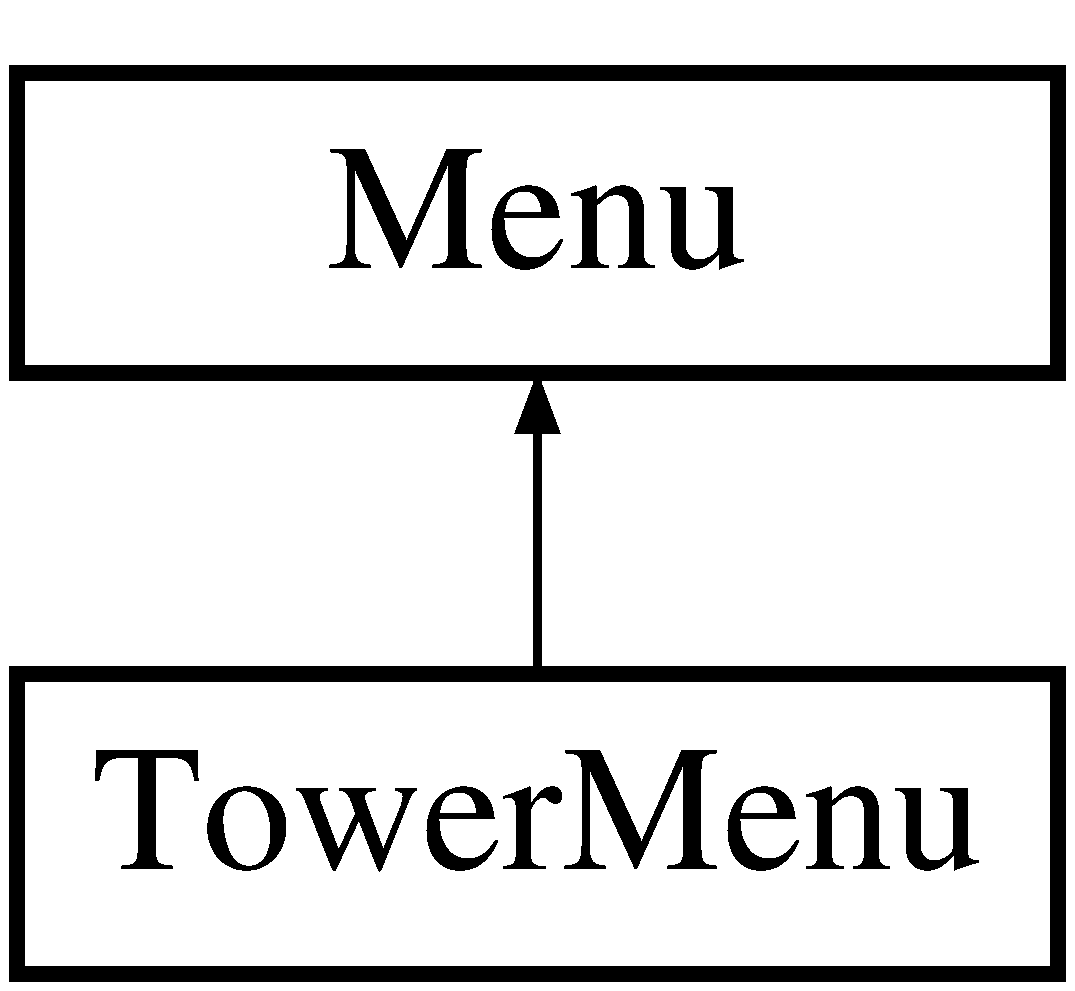
\includegraphics[height=2.000000cm]{class_tower_menu}
\end{center}
\end{figure}
\subsection*{Public Member Functions}
\begin{DoxyCompactItemize}
\item 
\hyperlink{class_tower_menu_aebdd08286832e919f6f379c79064615e}{Tower\+Menu} ()
\begin{DoxyCompactList}\small\item\em Default constructor. \end{DoxyCompactList}\item 
\hyperlink{class_tower_menu_afb563f251023dc6ad4b7ef17f4d3b46f}{Tower\+Menu} (shared\+\_\+ptr$<$ \hyperlink{class_tile}{Tile} $>$ t)
\begin{DoxyCompactList}\small\item\em Construct the build\+Menu at this tile. \end{DoxyCompactList}\item 
\hyperlink{class_tower_menu_adb6ddb7949289ce8e8e65323640acf7b}{$\sim$\+Tower\+Menu} ()
\begin{DoxyCompactList}\small\item\em Destructor. \end{DoxyCompactList}\item 
shared\+\_\+ptr$<$ \hyperlink{class_tile}{Tile} $>$ \hyperlink{class_tower_menu_a325d61a9e3cc201812eef18ac7ffad2d}{get\+Tile} ()
\begin{DoxyCompactList}\small\item\em Get the tile which opens the towermenu. \end{DoxyCompactList}\item 
void \hyperlink{class_tower_menu_aacd3732231059c039a663f98fd6ec349}{resolve\+Event} (sf\+::\+Event event)
\begin{DoxyCompactList}\small\item\em Resolve all the events on this tile. \end{DoxyCompactList}\item 
void \hyperlink{class_tower_menu_a32b70e92c85a41365360e8e46704bdf7}{sell\+Tower} ()
\begin{DoxyCompactList}\small\item\em Sell the tower in this tile. \end{DoxyCompactList}\item 
void \hyperlink{class_tower_menu_a0ecd4cdad69ed36c06781035d77569bc}{draw} (sf\+::\+Render\+Window \&)
\begin{DoxyCompactList}\small\item\em Draw the menu. \end{DoxyCompactList}\item 
void \hyperlink{class_tower_menu_afc1c7447eacd85abfa1f36ccdf3cbd7d}{close} ()
\begin{DoxyCompactList}\small\item\em Close the menu. \end{DoxyCompactList}\end{DoxyCompactItemize}
\subsection*{Additional Inherited Members}


\subsection{Detailed Description}
\hyperlink{class_tower}{Tower} \hyperlink{class_menu}{Menu} class. 

\subsection{Constructor \& Destructor Documentation}
\hypertarget{class_tower_menu_aebdd08286832e919f6f379c79064615e}{\index{Tower\+Menu@{Tower\+Menu}!Tower\+Menu@{Tower\+Menu}}
\index{Tower\+Menu@{Tower\+Menu}!Tower\+Menu@{Tower\+Menu}}
\subsubsection[{Tower\+Menu}]{\setlength{\rightskip}{0pt plus 5cm}Tower\+Menu\+::\+Tower\+Menu (
\begin{DoxyParamCaption}
{}
\end{DoxyParamCaption}
)}}\label{class_tower_menu_aebdd08286832e919f6f379c79064615e}


Default constructor. 

Default constructor. \hypertarget{class_tower_menu_afb563f251023dc6ad4b7ef17f4d3b46f}{\index{Tower\+Menu@{Tower\+Menu}!Tower\+Menu@{Tower\+Menu}}
\index{Tower\+Menu@{Tower\+Menu}!Tower\+Menu@{Tower\+Menu}}
\subsubsection[{Tower\+Menu}]{\setlength{\rightskip}{0pt plus 5cm}Tower\+Menu\+::\+Tower\+Menu (
\begin{DoxyParamCaption}
\item[{shared\+\_\+ptr$<$ {\bf Tile} $>$}]{t}
\end{DoxyParamCaption}
)}}\label{class_tower_menu_afb563f251023dc6ad4b7ef17f4d3b46f}


Construct the build\+Menu at this tile. 

\hypertarget{class_tower_menu_adb6ddb7949289ce8e8e65323640acf7b}{\index{Tower\+Menu@{Tower\+Menu}!````~Tower\+Menu@{$\sim$\+Tower\+Menu}}
\index{````~Tower\+Menu@{$\sim$\+Tower\+Menu}!Tower\+Menu@{Tower\+Menu}}
\subsubsection[{$\sim$\+Tower\+Menu}]{\setlength{\rightskip}{0pt plus 5cm}Tower\+Menu\+::$\sim$\+Tower\+Menu (
\begin{DoxyParamCaption}
{}
\end{DoxyParamCaption}
)}}\label{class_tower_menu_adb6ddb7949289ce8e8e65323640acf7b}


Destructor. 

Destructor. 

\subsection{Member Function Documentation}
\hypertarget{class_tower_menu_afc1c7447eacd85abfa1f36ccdf3cbd7d}{\index{Tower\+Menu@{Tower\+Menu}!close@{close}}
\index{close@{close}!Tower\+Menu@{Tower\+Menu}}
\subsubsection[{close}]{\setlength{\rightskip}{0pt plus 5cm}void Tower\+Menu\+::close (
\begin{DoxyParamCaption}
{}
\end{DoxyParamCaption}
)\hspace{0.3cm}{\ttfamily [virtual]}}}\label{class_tower_menu_afc1c7447eacd85abfa1f36ccdf3cbd7d}


Close the menu. 



Reimplemented from \hyperlink{class_menu_a4bc958c66bb39a91446b5c12ac6469c6}{Menu}.

\hypertarget{class_tower_menu_a0ecd4cdad69ed36c06781035d77569bc}{\index{Tower\+Menu@{Tower\+Menu}!draw@{draw}}
\index{draw@{draw}!Tower\+Menu@{Tower\+Menu}}
\subsubsection[{draw}]{\setlength{\rightskip}{0pt plus 5cm}void Tower\+Menu\+::draw (
\begin{DoxyParamCaption}
\item[{sf\+::\+Render\+Window \&}]{w}
\end{DoxyParamCaption}
)\hspace{0.3cm}{\ttfamily [virtual]}}}\label{class_tower_menu_a0ecd4cdad69ed36c06781035d77569bc}


Draw the menu. 



Reimplemented from \hyperlink{class_menu_a5c486201ec217b10588c145d043e4eb8}{Menu}.

\hypertarget{class_tower_menu_a325d61a9e3cc201812eef18ac7ffad2d}{\index{Tower\+Menu@{Tower\+Menu}!get\+Tile@{get\+Tile}}
\index{get\+Tile@{get\+Tile}!Tower\+Menu@{Tower\+Menu}}
\subsubsection[{get\+Tile}]{\setlength{\rightskip}{0pt plus 5cm}shared\+\_\+ptr$<$ {\bf Tile} $>$ Tower\+Menu\+::get\+Tile (
\begin{DoxyParamCaption}
{}
\end{DoxyParamCaption}
)}}\label{class_tower_menu_a325d61a9e3cc201812eef18ac7ffad2d}


Get the tile which opens the towermenu. 

\hypertarget{class_tower_menu_aacd3732231059c039a663f98fd6ec349}{\index{Tower\+Menu@{Tower\+Menu}!resolve\+Event@{resolve\+Event}}
\index{resolve\+Event@{resolve\+Event}!Tower\+Menu@{Tower\+Menu}}
\subsubsection[{resolve\+Event}]{\setlength{\rightskip}{0pt plus 5cm}void Tower\+Menu\+::resolve\+Event (
\begin{DoxyParamCaption}
\item[{sf\+::\+Event}]{event}
\end{DoxyParamCaption}
)\hspace{0.3cm}{\ttfamily [virtual]}}}\label{class_tower_menu_aacd3732231059c039a663f98fd6ec349}


Resolve all the events on this tile. 


\begin{DoxyParams}{Parameters}
{\em event} & the event to resolve. \\
\hline
\end{DoxyParams}


Implements \hyperlink{class_menu_a91ec4d6d898e740524b1fe3312d8f197}{Menu}.

\hypertarget{class_tower_menu_a32b70e92c85a41365360e8e46704bdf7}{\index{Tower\+Menu@{Tower\+Menu}!sell\+Tower@{sell\+Tower}}
\index{sell\+Tower@{sell\+Tower}!Tower\+Menu@{Tower\+Menu}}
\subsubsection[{sell\+Tower}]{\setlength{\rightskip}{0pt plus 5cm}void Tower\+Menu\+::sell\+Tower (
\begin{DoxyParamCaption}
{}
\end{DoxyParamCaption}
)}}\label{class_tower_menu_a32b70e92c85a41365360e8e46704bdf7}


Sell the tower in this tile. 



The documentation for this class was generated from the following files\+:\begin{DoxyCompactItemize}
\item 
D\+:/\+Tower\+Defense/\+Tower\+Defense/\hyperlink{_tower_menu_8h}{Tower\+Menu.\+h}\item 
D\+:/\+Tower\+Defense/\+Tower\+Defense/\hyperlink{_tower_menu_8cpp}{Tower\+Menu.\+cpp}\end{DoxyCompactItemize}

\hypertarget{class_wave}{\section{Wave Class Reference}
\label{class_wave}\index{Wave@{Wave}}
}


{\ttfamily \#include $<$Wave.\+h$>$}

\subsection*{Public Member Functions}
\begin{DoxyCompactItemize}
\item 
\hyperlink{class_wave_a3d8144ec0d6c0b0ede77ff59f54471aa}{Wave} ()
\item 
\hyperlink{class_wave_a774b08c0e12725a67094d5d1c3ed3553}{Wave} (vector$<$ shared\+\_\+ptr$<$ \hyperlink{class_enemy}{Enemy} $>$$>$)
\item 
\hyperlink{class_wave_a790eb8701e1bd20558b39cbafe20d36c}{Wave} (int line\+Number)
\item 
void \hyperlink{class_wave_a22532b46c406de513257a30e9f997264}{spawn\+Enemy} ()
\item 
void \hyperlink{class_wave_a7f2f45dca94480f64fe0ede4e7b53056}{add\+Enemy} (char type)
\item 
int \hyperlink{class_wave_a0b2ae90f612c1f8d0e7c595ac36092e6}{get\+Spawn\+Cooldown} ()
\end{DoxyCompactItemize}


\subsection{Constructor \& Destructor Documentation}
\hypertarget{class_wave_a3d8144ec0d6c0b0ede77ff59f54471aa}{\index{Wave@{Wave}!Wave@{Wave}}
\index{Wave@{Wave}!Wave@{Wave}}
\subsubsection[{Wave}]{\setlength{\rightskip}{0pt plus 5cm}Wave\+::\+Wave (
\begin{DoxyParamCaption}
{}
\end{DoxyParamCaption}
)}}\label{class_wave_a3d8144ec0d6c0b0ede77ff59f54471aa}
\hypertarget{class_wave_a774b08c0e12725a67094d5d1c3ed3553}{\index{Wave@{Wave}!Wave@{Wave}}
\index{Wave@{Wave}!Wave@{Wave}}
\subsubsection[{Wave}]{\setlength{\rightskip}{0pt plus 5cm}Wave\+::\+Wave (
\begin{DoxyParamCaption}
\item[{vector$<$ shared\+\_\+ptr$<$ {\bf Enemy} $>$$>$}]{e}
\end{DoxyParamCaption}
)}}\label{class_wave_a774b08c0e12725a67094d5d1c3ed3553}
\hypertarget{class_wave_a790eb8701e1bd20558b39cbafe20d36c}{\index{Wave@{Wave}!Wave@{Wave}}
\index{Wave@{Wave}!Wave@{Wave}}
\subsubsection[{Wave}]{\setlength{\rightskip}{0pt plus 5cm}Wave\+::\+Wave (
\begin{DoxyParamCaption}
\item[{int}]{line\+Number}
\end{DoxyParamCaption}
)}}\label{class_wave_a790eb8701e1bd20558b39cbafe20d36c}


\subsection{Member Function Documentation}
\hypertarget{class_wave_a7f2f45dca94480f64fe0ede4e7b53056}{\index{Wave@{Wave}!add\+Enemy@{add\+Enemy}}
\index{add\+Enemy@{add\+Enemy}!Wave@{Wave}}
\subsubsection[{add\+Enemy}]{\setlength{\rightskip}{0pt plus 5cm}void Wave\+::add\+Enemy (
\begin{DoxyParamCaption}
\item[{char}]{type}
\end{DoxyParamCaption}
)}}\label{class_wave_a7f2f45dca94480f64fe0ede4e7b53056}
\hypertarget{class_wave_a0b2ae90f612c1f8d0e7c595ac36092e6}{\index{Wave@{Wave}!get\+Spawn\+Cooldown@{get\+Spawn\+Cooldown}}
\index{get\+Spawn\+Cooldown@{get\+Spawn\+Cooldown}!Wave@{Wave}}
\subsubsection[{get\+Spawn\+Cooldown}]{\setlength{\rightskip}{0pt plus 5cm}int Wave\+::get\+Spawn\+Cooldown (
\begin{DoxyParamCaption}
{}
\end{DoxyParamCaption}
)}}\label{class_wave_a0b2ae90f612c1f8d0e7c595ac36092e6}
\hypertarget{class_wave_a22532b46c406de513257a30e9f997264}{\index{Wave@{Wave}!spawn\+Enemy@{spawn\+Enemy}}
\index{spawn\+Enemy@{spawn\+Enemy}!Wave@{Wave}}
\subsubsection[{spawn\+Enemy}]{\setlength{\rightskip}{0pt plus 5cm}void Wave\+::spawn\+Enemy (
\begin{DoxyParamCaption}
{}
\end{DoxyParamCaption}
)}}\label{class_wave_a22532b46c406de513257a30e9f997264}


The documentation for this class was generated from the following files\+:\begin{DoxyCompactItemize}
\item 
D\+:/\+Tower\+Defense/\+Tower\+Defense/\hyperlink{_wave_8h}{Wave.\+h}\item 
D\+:/\+Tower\+Defense/\+Tower\+Defense/\hyperlink{_wave_8cpp}{Wave.\+cpp}\end{DoxyCompactItemize}

\chapter{File Documentation}
\hypertarget{_area_attack_8cpp}{\section{D\+:/\+Tower\+Defense/\+Tower\+Defense/\+Area\+Attack.cpp File Reference}
\label{_area_attack_8cpp}\index{D\+:/\+Tower\+Defense/\+Tower\+Defense/\+Area\+Attack.\+cpp@{D\+:/\+Tower\+Defense/\+Tower\+Defense/\+Area\+Attack.\+cpp}}
}
{\ttfamily \#include \char`\"{}Area\+Attack.\+h\char`\"{}}\\*
{\ttfamily \#include \char`\"{}Level\+Manager.\+h\char`\"{}}\\*

\hypertarget{_area_attack_8h}{\section{D\+:/\+Tower\+Defense/\+Tower\+Defense/\+Area\+Attack.h File Reference}
\label{_area_attack_8h}\index{D\+:/\+Tower\+Defense/\+Tower\+Defense/\+Area\+Attack.\+h@{D\+:/\+Tower\+Defense/\+Tower\+Defense/\+Area\+Attack.\+h}}
}
{\ttfamily \#include \char`\"{}Attack.\+h\char`\"{}}\\*
\subsection*{Classes}
\begin{DoxyCompactItemize}
\item 
class \hyperlink{class_area_attack}{Area\+Attack}
\end{DoxyCompactItemize}

\hypertarget{_attack_8cpp}{\section{D\+:/\+Tower\+Defense/\+Tower\+Defense/\+Attack.cpp File Reference}
\label{_attack_8cpp}\index{D\+:/\+Tower\+Defense/\+Tower\+Defense/\+Attack.\+cpp@{D\+:/\+Tower\+Defense/\+Tower\+Defense/\+Attack.\+cpp}}
}
{\ttfamily \#include \char`\"{}Attack.\+h\char`\"{}}\\*
{\ttfamily \#include \char`\"{}Level\+Manager.\+h\char`\"{}}\\*
{\ttfamily \#include \char`\"{}Normal\+Enemy.\+h\char`\"{}}\\*
{\ttfamily \#include $<$memory$>$}\\*

\hypertarget{_attack_8h}{\section{D\+:/\+Tower\+Defense/\+Tower\+Defense/\+Attack.h File Reference}
\label{_attack_8h}\index{D\+:/\+Tower\+Defense/\+Tower\+Defense/\+Attack.\+h@{D\+:/\+Tower\+Defense/\+Tower\+Defense/\+Attack.\+h}}
}
{\ttfamily \#include $<$S\+F\+M\+L/\+Graphics.\+hpp$>$}\\*
{\ttfamily \#include \char`\"{}Enemy.\+h\char`\"{}}\\*
\subsection*{Classes}
\begin{DoxyCompactItemize}
\item 
class \hyperlink{class_attack}{Attack}
\end{DoxyCompactItemize}

\hypertarget{_audio_manager_8cpp}{\section{D\+:/\+Tower\+Defense/\+Tower\+Defense/\+Audio\+Manager.cpp File Reference}
\label{_audio_manager_8cpp}\index{D\+:/\+Tower\+Defense/\+Tower\+Defense/\+Audio\+Manager.\+cpp@{D\+:/\+Tower\+Defense/\+Tower\+Defense/\+Audio\+Manager.\+cpp}}
}
{\ttfamily \#include \char`\"{}Audio\+Manager.\+h\char`\"{}}\\*
{\ttfamily \#include $<$S\+F\+M\+L/\+Audio.\+hpp$>$}\\*
{\ttfamily \#include $<$S\+F\+M\+L/\+Audio/\+Music.\+hpp$>$}\\*
{\ttfamily \#include $<$memory$>$}\\*
{\ttfamily \#include \char`\"{}Config.\+h\char`\"{}}\\*
\subsection*{Variables}
\begin{DoxyCompactItemize}
\item 
sf\+::\+Music \hyperlink{_audio_manager_8cpp_a09e7f7edd9f51059c74373800ff69456}{music}
\end{DoxyCompactItemize}


\subsection{Variable Documentation}
\hypertarget{_audio_manager_8cpp_a09e7f7edd9f51059c74373800ff69456}{\index{Audio\+Manager.\+cpp@{Audio\+Manager.\+cpp}!music@{music}}
\index{music@{music}!Audio\+Manager.\+cpp@{Audio\+Manager.\+cpp}}
\subsubsection[{music}]{\setlength{\rightskip}{0pt plus 5cm}sf\+::\+Music music}}\label{_audio_manager_8cpp_a09e7f7edd9f51059c74373800ff69456}

\hypertarget{_audio_manager_8h}{\section{D\+:/\+Tower\+Defense/\+Tower\+Defense/\+Audio\+Manager.h File Reference}
\label{_audio_manager_8h}\index{D\+:/\+Tower\+Defense/\+Tower\+Defense/\+Audio\+Manager.\+h@{D\+:/\+Tower\+Defense/\+Tower\+Defense/\+Audio\+Manager.\+h}}
}
{\ttfamily \#include $<$memory$>$}\\*
\subsection*{Classes}
\begin{DoxyCompactItemize}
\item 
class \hyperlink{class_audio_manager}{Audio\+Manager}
\end{DoxyCompactItemize}

\hypertarget{_bomb_enemy_8cpp}{\section{D\+:/\+Tower\+Defense/\+Tower\+Defense/\+Bomb\+Enemy.cpp File Reference}
\label{_bomb_enemy_8cpp}\index{D\+:/\+Tower\+Defense/\+Tower\+Defense/\+Bomb\+Enemy.\+cpp@{D\+:/\+Tower\+Defense/\+Tower\+Defense/\+Bomb\+Enemy.\+cpp}}
}
{\ttfamily \#include \char`\"{}Bomb\+Enemy.\+h\char`\"{}}\\*
{\ttfamily \#include \char`\"{}Config.\+h\char`\"{}}\\*
{\ttfamily \#include \char`\"{}Tile.\+h\char`\"{}}\\*
{\ttfamily \#include \char`\"{}Field.\+h\char`\"{}}\\*
{\ttfamily \#include \char`\"{}Level\+Manager.\+h\char`\"{}}\\*

\hypertarget{_bomb_enemy_8h}{\section{D\+:/\+Tower\+Defense/\+Tower\+Defense/\+Bomb\+Enemy.h File Reference}
\label{_bomb_enemy_8h}\index{D\+:/\+Tower\+Defense/\+Tower\+Defense/\+Bomb\+Enemy.\+h@{D\+:/\+Tower\+Defense/\+Tower\+Defense/\+Bomb\+Enemy.\+h}}
}
{\ttfamily \#include \char`\"{}Enemy.\+h\char`\"{}}\\*
{\ttfamily \#include \char`\"{}Tile.\+h\char`\"{}}\\*
{\ttfamily \#include $<$S\+F\+M\+L\textbackslash{}\+Graphics.\+hpp$>$}\\*
{\ttfamily \#include $<$vector$>$}\\*
\subsection*{Classes}
\begin{DoxyCompactItemize}
\item 
class \hyperlink{class_bomb_enemy}{Bomb\+Enemy}
\end{DoxyCompactItemize}

\hypertarget{_build_menu_8cpp}{\section{D\+:/\+Tower\+Defense/\+Tower\+Defense/\+Build\+Menu.cpp File Reference}
\label{_build_menu_8cpp}\index{D\+:/\+Tower\+Defense/\+Tower\+Defense/\+Build\+Menu.\+cpp@{D\+:/\+Tower\+Defense/\+Tower\+Defense/\+Build\+Menu.\+cpp}}
}
{\ttfamily \#include \char`\"{}Build\+Menu.\+h\char`\"{}}\\*
{\ttfamily \#include \char`\"{}Config.\+h\char`\"{}}\\*
{\ttfamily \#include \char`\"{}Level\+Manager.\+h\char`\"{}}\\*
{\ttfamily \#include \char`\"{}Normal\+Tower.\+h\char`\"{}}\\*
{\ttfamily \#include \char`\"{}Money\+Tower.\+h\char`\"{}}\\*
{\ttfamily \#include \char`\"{}Slow\+Tower.\+h\char`\"{}}\\*
{\ttfamily \#include \char`\"{}Sun\+Tower.\+h\char`\"{}}\\*
{\ttfamily \#include \char`\"{}Tower.\+h\char`\"{}}\\*

\hypertarget{_build_menu_8h}{\section{D\+:/\+Tower\+Defense/\+Tower\+Defense/\+Build\+Menu.h File Reference}
\label{_build_menu_8h}\index{D\+:/\+Tower\+Defense/\+Tower\+Defense/\+Build\+Menu.\+h@{D\+:/\+Tower\+Defense/\+Tower\+Defense/\+Build\+Menu.\+h}}
}
{\ttfamily \#include $<$S\+F\+M\+L\textbackslash{}\+Graphics.\+hpp$>$}\\*
{\ttfamily \#include $<$memory$>$}\\*
{\ttfamily \#include $<$string$>$}\\*
{\ttfamily \#include \char`\"{}Menu.\+h\char`\"{}}\\*
{\ttfamily \#include \char`\"{}Button.\+h\char`\"{}}\\*
\subsection*{Classes}
\begin{DoxyCompactItemize}
\item 
class \hyperlink{class_build_menu}{Build\+Menu}
\end{DoxyCompactItemize}

\hypertarget{_button_8cpp}{\section{D\+:/\+Tower\+Defense/\+Tower\+Defense/\+Button.cpp File Reference}
\label{_button_8cpp}\index{D\+:/\+Tower\+Defense/\+Tower\+Defense/\+Button.\+cpp@{D\+:/\+Tower\+Defense/\+Tower\+Defense/\+Button.\+cpp}}
}
{\ttfamily \#include \char`\"{}Button.\+h\char`\"{}}\\*

\hypertarget{_button_8h}{\section{D\+:/\+Tower\+Defense/\+Tower\+Defense/\+Button.h File Reference}
\label{_button_8h}\index{D\+:/\+Tower\+Defense/\+Tower\+Defense/\+Button.\+h@{D\+:/\+Tower\+Defense/\+Tower\+Defense/\+Button.\+h}}
}
{\ttfamily \#include $<$S\+F\+M\+L/\+Graphics.\+hpp$>$}\\*
{\ttfamily \#include $<$string$>$}\\*
{\ttfamily \#include \char`\"{}Config.\+h\char`\"{}}\\*
\subsection*{Classes}
\begin{DoxyCompactItemize}
\item 
class \hyperlink{class_button}{Button}
\end{DoxyCompactItemize}

\hypertarget{_config_8cpp}{\section{D\+:/\+Tower\+Defense/\+Tower\+Defense/\+Config.cpp File Reference}
\label{_config_8cpp}\index{D\+:/\+Tower\+Defense/\+Tower\+Defense/\+Config.\+cpp@{D\+:/\+Tower\+Defense/\+Tower\+Defense/\+Config.\+cpp}}
}
{\ttfamily \#include \char`\"{}Config.\+h\char`\"{}}\\*
{\ttfamily \#include $<$S\+F\+M\+L\textbackslash{}\+Graphics.\+hpp$>$}\\*
\subsection*{Variables}
\begin{DoxyCompactItemize}
\item 
const int \hyperlink{_config_8cpp_a5e6ce0dd58078611570510dc4b8d81f3}{W\+I\+N\+D\+O\+W\+\_\+\+W\+I\+D\+T\+H} = 1100
\item 
const int \hyperlink{_config_8cpp_ab76d138fa589df9a65fc05eb3bd56073}{W\+I\+N\+D\+O\+W\+\_\+\+H\+E\+I\+G\+H\+T} = 600
\item 
const int \hyperlink{_config_8cpp_af2696afe64b43c7acbf32c457ac1a7dd}{B\+O\+R\+D\+E\+R\+\_\+\+S\+I\+Z\+E} = 30
\item 
const int \hyperlink{_config_8cpp_a3e2944dfb70e536e121deb89ee5046ba}{F\+R\+A\+M\+E\+\_\+\+R\+A\+T\+E} = 60
\item 
const string \hyperlink{_config_8cpp_a98a98b43a3c660a595644e21da370ea1}{M\+A\+I\+N\+\_\+\+B\+G\+M} = \char`\"{}music/test.\+ogg\char`\"{}
\item 
const int \hyperlink{_config_8cpp_a9308a8ccab88ca272b896567bf38e736}{T\+I\+L\+E\+\_\+\+W\+I\+D\+T\+H} = 50
\item 
const int \hyperlink{_config_8cpp_a42a5a878656c88718453eb9b65811231}{T\+I\+L\+E\+\_\+\+H\+E\+I\+G\+H\+T} = 50
\item 
const int \hyperlink{_config_8cpp_af1a31ec819c4de8e5cff1ec6621af8b0}{T\+I\+L\+E\+\_\+\+C\+O\+O\+L\+D\+O\+W\+N} = 240
\item 
const int \hyperlink{_config_8cpp_a344369233a6340f2cb8ecfa1ea440760}{T\+I\+L\+E\+\_\+\+N\+U\+M\+\_\+\+H\+O\+R} = 10
\item 
const int \hyperlink{_config_8cpp_a568ba188edc76e90788aeecc415d229f}{T\+I\+L\+E\+\_\+\+N\+U\+M\+\_\+\+V\+E\+R} = 20
\item 
const int \hyperlink{_config_8cpp_a4b610eb6047af0265a017721d8c05a85}{N\+U\+M\+\_\+\+S\+T\+A\+R\+T\+\_\+\+T\+I\+L\+E} = 4 $\ast$ \hyperlink{_config_8h_a568ba188edc76e90788aeecc415d229f}{T\+I\+L\+E\+\_\+\+N\+U\+M\+\_\+\+V\+E\+R}
\item 
const int \hyperlink{_config_8cpp_a5ba50ee35d29344c9c64096eab4b4e12}{N\+U\+M\+\_\+\+E\+N\+D\+\_\+\+T\+I\+L\+E} = 5 $\ast$ \hyperlink{_config_8h_a568ba188edc76e90788aeecc415d229f}{T\+I\+L\+E\+\_\+\+N\+U\+M\+\_\+\+V\+E\+R} -\/ 1
\item 
const string \hyperlink{_config_8cpp_a2b3536c09a1d7dd8bfb01973b06c4f3e}{T\+I\+L\+E\+\_\+\+S\+P\+R\+I\+T\+E} = \char`\"{}sprites/tile\+\_\+texture.\+png\char`\"{}
\item 
const int \hyperlink{_config_8cpp_ab132f0b66285780286c594be2037788b}{B\+U\+T\+T\+O\+N\+\_\+\+W\+I\+D\+T\+H} = 50
\item 
const int \hyperlink{_config_8cpp_a83f45a813d7a4cde3f8a9bb8a5a7d163}{B\+U\+T\+T\+O\+N\+\_\+\+H\+E\+I\+G\+H\+T} = 50
\item 
const int \hyperlink{_config_8cpp_ac1f1e08235a00c05a9a2b1068ea82c12}{W\+A\+V\+E\+\_\+\+T\+O\+T\+A\+L} = 15
\item 
const string \hyperlink{_config_8cpp_a1ba2d24e4ca25d71ce3e74e66c8d62d5}{W\+A\+V\+E\+\_\+\+F\+I\+L\+E\+\_\+\+A\+D\+D\+R\+E\+S\+S} = \char`\"{}Waves.\+txt\char`\"{}
\item 
const int \hyperlink{_config_8cpp_a6950a391b8d99f883ae9a4666d12b734}{W\+A\+V\+E\+\_\+\+S\+P\+A\+W\+N\+\_\+\+C\+O\+O\+L\+D\+O\+W\+N} = 10
\item 
const int \hyperlink{_config_8cpp_af699a40b1930195694d811d36ccbf796}{W\+A\+V\+E\+\_\+\+S\+P\+A\+W\+N\+\_\+\+P\+A\+U\+S\+E\+\_\+\+C\+O\+O\+L\+D\+O\+W\+N} = 100
\item 
const int \hyperlink{_config_8cpp_ae75186b01b0065a1dabe91696f0af4b1}{W\+A\+V\+E\+\_\+\+C\+O\+O\+L\+D\+O\+W\+N} = 300
\item 
const float \hyperlink{_config_8cpp_a256a8225ccb1f2d85369cab53fe9b2ff}{N\+O\+R\+M\+A\+L\+\_\+\+E\+N\+E\+M\+Y\+\_\+\+S\+P\+E\+E\+D} = 4
\item 
const int \hyperlink{_config_8cpp_a23266a8da450cd054f44ffa567d19e31}{N\+O\+R\+M\+A\+L\+\_\+\+E\+N\+E\+M\+Y\+\_\+\+H\+P} = 100
\item 
const int \hyperlink{_config_8cpp_a6aa2e8b289c78099943ae63cf6af69a7}{N\+O\+R\+M\+A\+L\+\_\+\+E\+N\+E\+M\+Y\+\_\+\+B\+O\+U\+N\+T\+Y} = 100
\item 
const int \hyperlink{_config_8cpp_af1fc1a8683d810a1f687d8482f2b1f28}{N\+O\+R\+M\+A\+L\+\_\+\+E\+N\+E\+M\+Y\+\_\+\+S\+C\+O\+R\+E\+V\+A\+L\+U\+E} = 100
\item 
const float \hyperlink{_config_8cpp_af099efedc5ec844c8f4551c8a132c8e3}{N\+O\+R\+M\+A\+L\+\_\+\+E\+N\+E\+M\+Y\+\_\+\+D\+E\+F\+E\+N\+C\+E} = 10
\item 
const string \hyperlink{_config_8cpp_a2f449bb7ddc57eb35c8bf9ed712e56d2}{N\+O\+R\+M\+A\+L\+\_\+\+E\+N\+E\+M\+Y\+\_\+\+S\+P\+R\+I\+T\+E\+\_\+\+A\+D\+D} = \char`\"{}sprites/enemies/basic\+\_\+enemy.\+png\char`\"{}
\item 
const float \hyperlink{_config_8cpp_a9b231072b8b108982b5e7f100ddd07dc}{F\+A\+S\+T\+\_\+\+E\+N\+E\+M\+Y\+\_\+\+S\+P\+E\+E\+D} = 10
\item 
const int \hyperlink{_config_8cpp_a94b36ddb1608edbf990d58a47f3d6e60}{F\+A\+S\+T\+\_\+\+E\+N\+E\+M\+Y\+\_\+\+H\+P} = 50
\item 
const int \hyperlink{_config_8cpp_af36d39835e6597181f7b8e36a9eb6085}{F\+A\+S\+T\+\_\+\+E\+N\+E\+M\+Y\+\_\+\+B\+O\+U\+N\+T\+Y} = 150
\item 
const int \hyperlink{_config_8cpp_a5a88eb50265321efe4bbb142ace5d9cc}{F\+A\+S\+T\+\_\+\+E\+N\+E\+M\+Y\+\_\+\+S\+C\+O\+R\+E\+V\+A\+L\+U\+E} = 150
\item 
const float \hyperlink{_config_8cpp_aed145fc4878b8ae7308433e837ffa0c3}{F\+A\+S\+T\+\_\+\+E\+N\+E\+M\+Y\+\_\+\+D\+E\+F\+E\+N\+C\+E} = 7
\item 
const string \hyperlink{_config_8cpp_ab9f685e62078c6d10ba0c34ca91e163a}{F\+A\+S\+T\+\_\+\+E\+N\+E\+M\+Y\+\_\+\+S\+P\+R\+I\+T\+E\+\_\+\+A\+D\+D} = \char`\"{}sprites/enemies/fast\+\_\+enemy.\+png\char`\"{}
\item 
const float \hyperlink{_config_8cpp_a1becdc757ef68f876fe4bc7d683b58f3}{B\+O\+M\+B\+\_\+\+E\+N\+E\+M\+Y\+\_\+\+S\+P\+E\+E\+D} = 5
\item 
const int \hyperlink{_config_8cpp_a006682436ed543ebbbfdd593f3fb8032}{B\+O\+M\+B\+\_\+\+E\+N\+E\+M\+Y\+\_\+\+H\+P} = 5000
\item 
const int \hyperlink{_config_8cpp_aec10e5fdfd476e5a46f9ec2dc175ab56}{B\+O\+M\+B\+\_\+\+E\+N\+E\+M\+Y\+\_\+\+B\+O\+U\+N\+T\+Y} = 100
\item 
const int \hyperlink{_config_8cpp_adfdc1c3370eb8fd0c50bb4ae44b4ffab}{B\+O\+M\+B\+\_\+\+E\+N\+E\+M\+Y\+\_\+\+S\+C\+O\+R\+E\+V\+A\+L\+U\+E} = 200
\item 
const float \hyperlink{_config_8cpp_a09858a1b9491be66f2ca9035d33a2f79}{B\+O\+M\+B\+\_\+\+E\+N\+E\+M\+Y\+\_\+\+D\+E\+F\+E\+N\+C\+E} = 15
\item 
const string \hyperlink{_config_8cpp_a6758f00ef5dfcde25ffc6dbc0ca1dcf8}{B\+O\+M\+B\+\_\+\+E\+N\+E\+M\+Y\+\_\+\+S\+P\+R\+I\+T\+E\+\_\+\+A\+D\+D} = \char`\"{}sprites/enemies/bomb\+\_\+enemy.\+png\char`\"{}
\item 
const int \hyperlink{_config_8cpp_a7231359eb0a40dceeeff5d1167aec991}{B\+O\+M\+B\+\_\+\+E\+N\+E\+M\+Y\+\_\+\+T\+R\+I\+G\+G\+E\+R} = 4800
\item 
const int \hyperlink{_config_8cpp_a0460729e91634f6e34187f8e48d04e43}{B\+O\+M\+B\+\_\+\+E\+N\+E\+M\+Y\+\_\+\+C\+O\+U\+N\+T\+D\+O\+W\+N} = 120
\item 
const float \hyperlink{_config_8cpp_ab585022c753f29cebbaffdbd3a28ea5f}{T\+O\+U\+G\+H\+\_\+\+E\+N\+E\+M\+Y\+\_\+\+S\+P\+E\+E\+D} = 2
\item 
const int \hyperlink{_config_8cpp_ac1ffe92f0482cbfb3a83a54818739eb9}{T\+O\+U\+G\+H\+\_\+\+E\+N\+E\+M\+Y\+\_\+\+H\+P} = 500
\item 
const int \hyperlink{_config_8cpp_a90e063ad420d70f4b13c390bc3b8ec3d}{T\+O\+U\+G\+H\+\_\+\+E\+N\+E\+M\+Y\+\_\+\+B\+O\+U\+N\+T\+Y} = 300
\item 
const int \hyperlink{_config_8cpp_a47ecddb7ea38a5582351dca6f864c7fd}{T\+O\+U\+G\+H\+\_\+\+E\+N\+E\+M\+Y\+\_\+\+S\+C\+O\+R\+E\+V\+A\+L\+U\+E} = 350
\item 
const float \hyperlink{_config_8cpp_aad3f3a3b10fb4c64b91225b983526097}{T\+O\+U\+G\+H\+\_\+\+E\+N\+E\+M\+Y\+\_\+\+D\+E\+F\+E\+N\+C\+E} = 10
\item 
const string \hyperlink{_config_8cpp_aa4fdb89dba30b28e81137ce7056fcb84}{T\+O\+U\+G\+H\+\_\+\+E\+N\+E\+M\+Y\+\_\+\+S\+P\+R\+I\+T\+E\+\_\+\+A\+D\+D} = \char`\"{}sprites/enemies/tough\+\_\+enemy.\+png\char`\"{}
\item 
const sf\+::\+Color \hyperlink{_config_8cpp_ac7f547170e82cfb5a58fd28cde85db9e}{R\+A\+N\+G\+E\+\_\+\+C\+I\+R\+C\+L\+E\+\_\+\+F\+I\+L\+L\+\_\+\+C\+O\+L\+O\+R} = sf\+::\+Color(0, 0, 255, 100)
\item 
const int \hyperlink{_config_8cpp_a9e9d9551618f57239f1e1ae0fa9c82c3}{T\+O\+W\+E\+R\+\_\+\+S\+P\+E\+E\+D} = 15
\item 
const float \hyperlink{_config_8cpp_abd616a32a6b1368e59ad09a7d37d9507}{N\+O\+R\+M\+A\+L\+\_\+\+T\+O\+W\+E\+R\+\_\+\+D\+A\+M\+A\+G\+E} \mbox{[}3\mbox{]} = \{ 10, 20, 25 \}
\item 
const int \hyperlink{_config_8cpp_a4d10326b360d9aa36c0835c7dbeee73f}{N\+O\+R\+M\+A\+L\+\_\+\+T\+O\+W\+E\+R\+\_\+\+S\+L\+O\+W\+\_\+\+A\+M\+O\+U\+N\+T} \mbox{[}3\mbox{]} = \{ 0, 0, 0 \}
\item 
const int \hyperlink{_config_8cpp_ae1eb195746f44940b2b0a2248a22f445}{N\+O\+R\+M\+A\+L\+\_\+\+T\+O\+W\+E\+R\+\_\+\+S\+P\+E\+E\+D} \mbox{[}3\mbox{]} = \{20, 15, 10\}
\item 
const float \hyperlink{_config_8cpp_a5c42843d0731d470a949c53613679958}{N\+O\+R\+M\+A\+L\+\_\+\+T\+O\+W\+E\+R\+\_\+\+R\+A\+N\+G\+E} \mbox{[}3\mbox{]} = \{ 125, 175, 225 \}
\item 
const int \hyperlink{_config_8cpp_ac7a9b5b51bebb564644228c2bd75a3f4}{N\+O\+R\+M\+A\+L\+\_\+\+T\+O\+W\+E\+R\+\_\+\+P\+R\+I\+C\+E} = 200
\item 
const int \hyperlink{_config_8cpp_afba04d39f1f2baad43d81121baeebeeb}{N\+O\+R\+M\+A\+L\+\_\+\+T\+O\+W\+E\+R\+\_\+\+I\+N\+C\+O\+M\+E} \mbox{[}3\mbox{]} = \{150,300, 450 \}
\item 
const string \hyperlink{_config_8cpp_a873e177b3bd65b8ecd6c70563d8062e1}{N\+O\+R\+M\+A\+L\+\_\+\+T\+O\+W\+E\+R\+\_\+\+S\+P\+R\+I\+T\+E\+\_\+\+A\+D\+D} = \char`\"{}sprites/normal\+\_\+tower.\+png\char`\"{}
\item 
const float \hyperlink{_config_8cpp_a5fcb6548f77ae3022771432785344dd0}{S\+U\+N\+\_\+\+T\+O\+W\+E\+R\+\_\+\+D\+A\+M\+A\+G\+E} \mbox{[}3\mbox{]} = \{ 25, 45, 60\}
\item 
const int \hyperlink{_config_8cpp_a2c145283c261b75fac3142a593c80aa2}{S\+U\+N\+\_\+\+T\+O\+W\+E\+R\+\_\+\+S\+L\+O\+W\+\_\+\+A\+M\+O\+U\+N\+T} \mbox{[}3\mbox{]} = \{ 0, 0, 0 \}
\item 
const int \hyperlink{_config_8cpp_a429a8c124db0f949b5d4ab7b904f6766}{S\+U\+N\+\_\+\+T\+O\+W\+E\+R\+\_\+\+S\+P\+E\+E\+D} \mbox{[}3\mbox{]} = \{60, 40, 20\}
\item 
const float \hyperlink{_config_8cpp_adad1098323d8d600ce00ff6730680b94}{S\+U\+N\+\_\+\+T\+O\+W\+E\+R\+\_\+\+R\+A\+N\+G\+E} \mbox{[}3\mbox{]} = \{ 125, 175, 225 \}
\item 
const int \hyperlink{_config_8cpp_a53355cb497c5d64acda04aedcbc9a8fb}{S\+U\+N\+\_\+\+T\+O\+W\+E\+R\+\_\+\+P\+R\+I\+C\+E} = 500
\item 
const int \hyperlink{_config_8cpp_a13ba8f77d3115f65a07b0a99f3a57460}{S\+U\+N\+\_\+\+T\+O\+W\+E\+R\+\_\+\+I\+N\+C\+O\+M\+E} \mbox{[}3\mbox{]} = \{400, 800, 1200\}
\item 
const string \hyperlink{_config_8cpp_af97b5bb409ea0f93a6fa5734941f4c6c}{S\+U\+N\+\_\+\+T\+O\+W\+E\+R\+\_\+\+S\+P\+R\+I\+T\+E\+\_\+\+A\+D\+D} = \char`\"{}sprites/sun\+\_\+tower.\+png\char`\"{}
\item 
const float \hyperlink{_config_8cpp_a6bbcbf4b294fa8bd3380dfdbffd38bf2}{M\+O\+N\+E\+Y\+\_\+\+T\+O\+W\+E\+R\+\_\+\+D\+A\+M\+A\+G\+E} \mbox{[}3\mbox{]} = \{ 0, 0, 0 \}
\item 
const int \hyperlink{_config_8cpp_a01aa7d73de9efef575fe306d4940c094}{M\+O\+N\+E\+Y\+\_\+\+T\+O\+W\+E\+R\+\_\+\+G\+E\+N\+E\+R\+A\+T\+I\+O\+N\+\_\+\+U\+N\+I\+T} \mbox{[}3\mbox{]} = \{ 300, 600, 900 \}
\item 
const int \hyperlink{_config_8cpp_afff6ca1b1a1c93ef6e9aa50f90e6f4cd}{M\+O\+N\+E\+Y\+\_\+\+T\+O\+W\+E\+R\+\_\+\+S\+P\+E\+E\+D} \mbox{[}3\mbox{]} = \{180, 150, 120\}
\item 
const float \hyperlink{_config_8cpp_a34aa462eae9cd6bd04ec1fbb2fc41fa0}{M\+O\+N\+E\+Y\+\_\+\+T\+O\+W\+E\+R\+\_\+\+R\+A\+N\+G\+E} \mbox{[}3\mbox{]} = \{ 0, 0, 0 \}
\item 
const int \hyperlink{_config_8cpp_ab5f86e498edb50b0cc41c595860b64dd}{M\+O\+N\+E\+Y\+\_\+\+T\+O\+W\+E\+R\+\_\+\+P\+R\+I\+C\+E} = 400
\item 
const int \hyperlink{_config_8cpp_a2d0c7f6347b30a1dd5f0aead217bde1d}{M\+O\+N\+E\+Y\+\_\+\+T\+O\+W\+E\+R\+\_\+\+I\+N\+C\+O\+M\+E} \mbox{[}3\mbox{]} = \{300, 600, 900\}
\item 
const string \hyperlink{_config_8cpp_a560c8e2451fbfdbb7837b8f751472f75}{M\+O\+N\+E\+Y\+\_\+\+T\+O\+W\+E\+R\+\_\+\+S\+P\+R\+I\+T\+E\+\_\+\+A\+D\+D} = \char`\"{}sprites/money\+\_\+tower.\+png\char`\"{}
\item 
const float \hyperlink{_config_8cpp_a59d61bde4846a3457476372036943e25}{S\+L\+O\+W\+\_\+\+T\+O\+W\+E\+R\+\_\+\+D\+A\+M\+A\+G\+E} \mbox{[}3\mbox{]} = \{ 0, 0, 0 \}
\item 
const int \hyperlink{_config_8cpp_a3e648d7e6d3dbc1cf5f9153368f5d7b1}{S\+L\+O\+W\+\_\+\+T\+O\+W\+E\+R\+\_\+\+S\+L\+O\+W\+\_\+\+A\+M\+O\+U\+N\+T} \mbox{[}3\mbox{]} = \{ 120, 180, 240 \}
\item 
const int \hyperlink{_config_8cpp_a60d027b1163faccd5ed1121aff71cb89}{S\+L\+O\+W\+\_\+\+T\+O\+W\+E\+R\+\_\+\+S\+P\+E\+E\+D} \mbox{[}3\mbox{]} = \{20, 15, 10\}
\item 
const float \hyperlink{_config_8cpp_a845780276cfd4cc149c39f793eee3ad7}{S\+L\+O\+W\+\_\+\+T\+O\+W\+E\+R\+\_\+\+R\+A\+N\+G\+E} \mbox{[}3\mbox{]} = \{ 125, 175, 225 \}
\item 
const int \hyperlink{_config_8cpp_ab096105fec1b1ff0e95befeaea108b4a}{S\+L\+O\+W\+\_\+\+T\+O\+W\+E\+R\+\_\+\+P\+R\+I\+C\+E} = 300
\item 
const int \hyperlink{_config_8cpp_aaf5f2e46c20dea7343a6c090f3f751c7}{S\+L\+O\+W\+\_\+\+T\+O\+W\+E\+R\+\_\+\+I\+N\+C\+O\+M\+E} \mbox{[}3\mbox{]} = \{250, 500, 750\}
\item 
const string \hyperlink{_config_8cpp_aac613d3ed3069e502f38674d63733083}{S\+L\+O\+W\+\_\+\+T\+O\+W\+E\+R\+\_\+\+S\+P\+R\+I\+T\+E\+\_\+\+A\+D\+D} = \char`\"{}sprites/slow\+\_\+tower.\+png\char`\"{}
\item 
const int \hyperlink{_config_8cpp_a68598a31bfe59e1ac25a63e7545bf68e}{S\+L\+O\+W\+\_\+\+E\+F\+F\+E\+C\+T} = 1
\item 
const string \hyperlink{_config_8cpp_a5561952d9be5290da418841839a3fca8}{G\+A\+M\+E\+\_\+\+M\+E\+N\+U\+\_\+\+D\+E\+F\+A\+U\+L\+T\+\_\+\+T\+E\+X\+T\+U\+R\+E} = \char`\"{}sprites/backgrounds/gamebg.\+png\char`\"{}
\item 
const string \hyperlink{_config_8cpp_abb4ef9294f60c5b6df6c2793acd40421}{S\+T\+A\+R\+T\+\_\+\+M\+E\+N\+U\+\_\+\+T\+E\+X\+T\+U\+R\+E} = \char`\"{}sprites/backgrounds/background.\+png\char`\"{}
\item 
const string \hyperlink{_config_8cpp_a0e4fd9320e2273cd6c9466d62418455a}{C\+R\+E\+D\+I\+T\+S\+\_\+\+S\+P\+R\+I\+T\+E\+\_\+\+A\+D\+D} = \char`\"{}sprites/backgrounds/credits.\+png\char`\"{}
\item 
const string \hyperlink{_config_8cpp_ad33eebe70df228c8676b1bef073f6cc7}{G\+A\+M\+E\+O\+V\+E\+R\+\_\+\+M\+E\+N\+U\+\_\+\+T\+E\+X\+T\+U\+R\+E} = \char`\"{}sprites/backgrounds/gameover.\+png\char`\"{}
\item 
const string \hyperlink{_config_8cpp_a9bcfcb5ec97dafe04a106184589428b6}{W\+I\+N\+\_\+\+M\+E\+N\+U\+\_\+\+T\+E\+X\+T\+U\+R\+E} =\char`\"{}sprites/youwin.\+png\char`\"{}
\item 
const string \hyperlink{_config_8cpp_ab63134a5f1b23019cd8494637b264145}{F\+O\+N\+T} = \char`\"{}ressources/Source\+Code\+Pro.\+ttf\char`\"{}
\item 
const sf\+::\+Vector2f \hyperlink{_config_8cpp_a8b8e59f62fbdc0ebd9ad4132336eea13}{L\+I\+F\+E\+\_\+\+C\+O\+U\+N\+T\+\_\+\+D\+I\+S\+P\+L\+A\+Y\+\_\+\+P\+O\+S\+I\+T\+I\+O\+N} = sf\+::\+Vector2f(500, 13)
\item 
const sf\+::\+Vector2f \hyperlink{_config_8cpp_ac1b3b6db5ef4be164fe14b315ce3180e}{P\+O\+I\+N\+T\+S\+\_\+\+C\+O\+U\+N\+T\+\_\+\+D\+I\+S\+P\+L\+A\+Y\+\_\+\+P\+O\+S\+I\+T\+I\+O\+N} = sf\+::\+Vector2f(700, 13)
\item 
const sf\+::\+Vector2f \hyperlink{_config_8cpp_a98de9cfc1924706e8b80e163b58d016c}{W\+A\+V\+E\+\_\+\+C\+O\+U\+N\+T\+\_\+\+D\+I\+S\+P\+L\+A\+Y\+\_\+\+P\+O\+S\+I\+T\+I\+O\+N} = sf\+::\+Vector2f(1000, 13)
\item 
const sf\+::\+Vector2f \hyperlink{_config_8cpp_a513a458aab31e002dcdb3b3bc4bb1d9b}{M\+O\+N\+E\+Y\+\_\+\+C\+O\+U\+N\+T\+\_\+\+D\+I\+S\+P\+L\+A\+Y\+\_\+\+P\+O\+S\+I\+T\+I\+O\+N} = sf\+::\+Vector2f(850, 13)
\item 
const string \hyperlink{_config_8cpp_a160c5ce1ef58346d0a7c90c4b501fe87}{P\+A\+U\+S\+E\+\_\+\+B\+U\+T\+T\+O\+N\+\_\+\+T\+E\+X\+T\+U\+R\+E} = \char`\"{}sprites/buttons/pause\+\_\+button.\+png\char`\"{}
\item 
const string \hyperlink{_config_8cpp_a504f7c5300cc4e427d1d994ce38ffa80}{S\+P\+E\+E\+D\+\_\+\+B\+U\+T\+T\+O\+N\+\_\+\+T\+E\+X\+T\+U\+R\+E} = \char`\"{}sprites/buttons/speed\+\_\+button.\+png\char`\"{}
\item 
const string \hyperlink{_config_8cpp_a0deebdf22893cd8ff57e71127df12abd}{M\+U\+T\+E\+\_\+\+B\+U\+T\+T\+O\+N\+\_\+\+T\+E\+X\+T\+U\+R\+E} = \char`\"{}sprites/buttons/mute\+\_\+button.\+png\char`\"{}
\item 
const string \hyperlink{_config_8cpp_a5f5fe05c34942c083a2bd7ec36c42e65}{R\+E\+S\+T\+A\+R\+T\+\_\+\+B\+U\+T\+T\+O\+N\+\_\+\+T\+E\+X\+T\+U\+R\+E} = \char`\"{}sprites/buttons/restart\+\_\+button.\+png\char`\"{}
\item 
const string \hyperlink{_config_8cpp_a16205d17ad81079f60abdb3eeccbb71b}{G\+I\+V\+E\+\_\+\+U\+P\+\_\+\+B\+U\+T\+T\+O\+N\+\_\+\+T\+E\+X\+T\+U\+R\+E} = \char`\"{}sprites/buttons/give\+\_\+up\+\_\+button.\+png\char`\"{}
\item 
const string \hyperlink{_config_8cpp_afcff1bd8ad71d22f2e54d1e6decacbd6}{S\+T\+A\+R\+T\+\_\+\+G\+A\+M\+E\+\_\+\+B\+U\+T\+T\+O\+N\+\_\+\+T\+E\+X\+T\+U\+R\+E} = \char`\"{}sprites/buttons/start\+\_\+game\+\_\+button.\+png\char`\"{}
\item 
const string \hyperlink{_config_8cpp_a4c67c75dde69775a1592adb2db45974e}{S\+C\+O\+R\+E\+B\+O\+A\+R\+D\+\_\+\+B\+U\+T\+T\+O\+N\+\_\+\+T\+E\+X\+T\+U\+R\+E} = \char`\"{}\char`\"{}
\item 
const string \hyperlink{_config_8cpp_a6dbdd1d3d1c730b51227257f972eac66}{C\+R\+E\+D\+I\+T\+S\+\_\+\+B\+U\+T\+T\+O\+N\+\_\+\+T\+E\+X\+T\+U\+R\+E} = \char`\"{}sprites/buttons/credits\+\_\+button.\+png\char`\"{}
\item 
const string \hyperlink{_config_8cpp_a584b13065b00cc0980a0dd179b5cd776}{E\+X\+I\+T\+\_\+\+G\+A\+M\+E\+\_\+\+B\+U\+T\+T\+O\+N\+\_\+\+T\+E\+X\+T\+U\+R\+E} = \char`\"{}sprites/buttons/exit\+\_\+game.\+png\char`\"{}
\item 
const string \hyperlink{_config_8cpp_a56be9d3bb20162697abbb892803393fa}{B\+A\+C\+K\+\_\+\+B\+U\+T\+T\+O\+N\+\_\+\+T\+E\+X\+T\+U\+R\+E} = \char`\"{}sprites/buttons/back\+\_\+button.\+png\char`\"{}
\item 
const string \hyperlink{_config_8cpp_a0f907c3d62d6e09de11b5fb0a1a063ca}{B\+A\+S\+I\+C\+\_\+\+T\+O\+W\+E\+R\+\_\+\+B\+U\+T\+T\+O\+N\+\_\+\+T\+E\+X\+T\+U\+R\+E} = \char`\"{}sprites/normal\+\_\+tower\+\_\+button.\+png\char`\"{}
\item 
const string \hyperlink{_config_8cpp_aee96d0862a35e2fd907311056892c132}{S\+U\+N\+\_\+\+T\+O\+W\+E\+R\+\_\+\+B\+U\+T\+T\+O\+N\+\_\+\+T\+E\+X\+T\+U\+R\+E} = \char`\"{}sprites/sun\+\_\+tower\+\_\+button.\+png\char`\"{}
\item 
const string \hyperlink{_config_8cpp_a65be6666522ac5ae13a2d18d35360ffb}{S\+L\+O\+W\+\_\+\+T\+O\+W\+E\+R\+\_\+\+B\+U\+T\+T\+O\+N\+\_\+\+T\+E\+X\+T\+U\+R\+E} = \char`\"{}sprites/slow\+\_\+tower\+\_\+button.\+png\char`\"{}
\item 
const string \hyperlink{_config_8cpp_acd41fcaa1b13647294a31e2ed3296e51}{M\+O\+N\+E\+Y\+\_\+\+T\+O\+W\+E\+R\+\_\+\+B\+U\+T\+T\+O\+N\+\_\+\+T\+E\+X\+T\+U\+R\+E} = \char`\"{}sprites/money\+\_\+tower\+\_\+button.\+png\char`\"{}
\item 
const string \hyperlink{_config_8cpp_acfab5205a2a0309f2bea49f75f47f14d}{S\+E\+L\+L\+\_\+\+B\+U\+T\+T\+O\+N\+\_\+\+T\+E\+X\+T\+U\+R\+E} = \char`\"{}sprites/sell\+\_\+tower\+\_\+button.\+png\char`\"{}
\item 
const string \hyperlink{_config_8cpp_ad1d8ab706e4e510d1c873684da5bba98}{U\+P\+G\+R\+A\+D\+E\+\_\+\+B\+U\+T\+T\+O\+N\+\_\+\+T\+E\+X\+T\+U\+R\+E} = \char`\"{}sprites/upgrade\+\_\+tower\+\_\+button.\+png\char`\"{}
\item 
const sf\+::\+Vector2i \hyperlink{_config_8cpp_a9163727e59245b727ff59fd6a4ac9dcb}{B\+U\+T\+T\+O\+N\+\_\+\+S\+I\+Z\+E} = sf\+::\+Vector2i(408, 76)
\item 
const sf\+::\+Vector2i \hyperlink{_config_8cpp_a3830c784f4b59ae4afa27986d46fb4c3}{M\+U\+T\+E\+\_\+\+B\+U\+T\+T\+O\+N\+\_\+\+S\+I\+Z\+E} = sf\+::\+Vector2i(100, 32)
\item 
const sf\+::\+Vector2i \hyperlink{_config_8cpp_a6d17e915dd53acc5d44a9478a54cc50a}{B\+A\+C\+K\+\_\+\+B\+U\+T\+T\+O\+N\+\_\+\+S\+I\+Z\+E} = sf\+::\+Vector2i(100, 34)
\item 
const sf\+::\+Vector2i \hyperlink{_config_8cpp_a6d124414f6c067a8f1c0069b646532ba}{S\+M\+A\+L\+L\+\_\+\+B\+U\+T\+T\+O\+N\+\_\+\+S\+I\+Z\+E} = sf\+::\+Vector2i(\hyperlink{_config_8h_ab132f0b66285780286c594be2037788b}{B\+U\+T\+T\+O\+N\+\_\+\+W\+I\+D\+T\+H}, \hyperlink{_config_8h_a83f45a813d7a4cde3f8a9bb8a5a7d163}{B\+U\+T\+T\+O\+N\+\_\+\+H\+E\+I\+G\+H\+T})
\item 
const sf\+::\+Vector2i \hyperlink{_config_8cpp_a1f1b9324cc7df80a91329f862cb448fd}{S\+T\+A\+R\+T\+\_\+\+B\+U\+T\+T\+O\+N\+\_\+\+P\+O\+S\+I\+T\+I\+O\+N} = sf\+::\+Vector2i(346, 150)
\item 
const sf\+::\+Vector2i \hyperlink{_config_8cpp_a8071b8ef5748081c7d148e8adf40f43c}{C\+R\+E\+D\+I\+T\+S\+\_\+\+B\+U\+T\+T\+O\+N\+\_\+\+P\+O\+S\+I\+T\+I\+O\+N} = sf\+::\+Vector2i(346, 250)
\item 
const sf\+::\+Vector2i \hyperlink{_config_8cpp_af71c764af82c72109856a042b789a0cb}{E\+X\+I\+T\+\_\+\+B\+U\+T\+T\+O\+N\+\_\+\+P\+O\+S\+I\+T\+I\+O\+N} = sf\+::\+Vector2i(346, 350)
\item 
const sf\+::\+Vector2i \hyperlink{_config_8cpp_acf3c7e2cee0db4dce014f46a116383ea}{M\+U\+T\+E\+\_\+\+B\+U\+T\+T\+O\+N\+\_\+\+P\+O\+S\+I\+T\+I\+O\+N} = sf\+::\+Vector2i(10, 10)
\item 
const sf\+::\+Vector2i \hyperlink{_config_8cpp_acd18e28e868333361c2494fe9f2a464a}{R\+E\+S\+T\+A\+R\+T\+\_\+\+B\+U\+T\+T\+O\+N\+\_\+\+P\+O\+S\+I\+T\+I\+O\+N} = sf\+::\+Vector2i(10, 560)
\item 
const sf\+::\+Vector2i \hyperlink{_config_8cpp_a21853d89bf8b839810045b3eb12e5747}{B\+A\+C\+K\+\_\+\+B\+U\+T\+T\+O\+N\+\_\+\+P\+O\+S\+I\+T\+I\+O\+N} = sf\+::\+Vector2i((\hyperlink{_config_8h_a5e6ce0dd58078611570510dc4b8d81f3}{W\+I\+N\+D\+O\+W\+\_\+\+W\+I\+D\+T\+H} -\/ M\+U\+T\+E\+\_\+\+B\+U\+T\+T\+O\+N\+\_\+\+S\+I\+Z\+E.\+x)/2,500)
\item 
const sf\+::\+Vector2i \hyperlink{_config_8cpp_a7606768f63d84716b31722ba7c099e61}{G\+O\+\_\+\+R\+E\+S\+T\+A\+R\+T\+\_\+\+B\+U\+T\+T\+O\+N\+\_\+\+P\+O\+S\+I\+T\+I\+O\+N} = sf\+::\+Vector2i(((\hyperlink{_config_8h_a5e6ce0dd58078611570510dc4b8d81f3}{W\+I\+N\+D\+O\+W\+\_\+\+W\+I\+D\+T\+H} -\/ M\+U\+T\+E\+\_\+\+B\+U\+T\+T\+O\+N\+\_\+\+S\+I\+Z\+E.\+x) / 2)+100, 500)
\item 
const sf\+::\+Vector2i \hyperlink{_config_8cpp_ab0c2f5d90a7a608c1e89b65fe670b818}{G\+O\+\_\+\+B\+A\+C\+K\+\_\+\+B\+U\+T\+T\+O\+N\+\_\+\+P\+O\+S\+I\+T\+I\+O\+N} = sf\+::\+Vector2i(((\hyperlink{_config_8h_a5e6ce0dd58078611570510dc4b8d81f3}{W\+I\+N\+D\+O\+W\+\_\+\+W\+I\+D\+T\+H} -\/ M\+U\+T\+E\+\_\+\+B\+U\+T\+T\+O\+N\+\_\+\+S\+I\+Z\+E.\+x) / 2) -\/ 100, 500)
\item 
const int \hyperlink{_config_8cpp_ab0e5764df7c0925df42c0de07cc26188}{I\+N\+I\+T\+\_\+\+M\+O\+N\+E\+Y} = 400
\item 
const int \hyperlink{_config_8cpp_aa3749ecd25214ba8202504d512ed7769}{I\+N\+I\+T\+\_\+\+H\+P} = 10
\end{DoxyCompactItemize}


\subsection{Variable Documentation}
\hypertarget{_config_8cpp_a21853d89bf8b839810045b3eb12e5747}{\index{Config.\+cpp@{Config.\+cpp}!B\+A\+C\+K\+\_\+\+B\+U\+T\+T\+O\+N\+\_\+\+P\+O\+S\+I\+T\+I\+O\+N@{B\+A\+C\+K\+\_\+\+B\+U\+T\+T\+O\+N\+\_\+\+P\+O\+S\+I\+T\+I\+O\+N}}
\index{B\+A\+C\+K\+\_\+\+B\+U\+T\+T\+O\+N\+\_\+\+P\+O\+S\+I\+T\+I\+O\+N@{B\+A\+C\+K\+\_\+\+B\+U\+T\+T\+O\+N\+\_\+\+P\+O\+S\+I\+T\+I\+O\+N}!Config.\+cpp@{Config.\+cpp}}
\subsubsection[{B\+A\+C\+K\+\_\+\+B\+U\+T\+T\+O\+N\+\_\+\+P\+O\+S\+I\+T\+I\+O\+N}]{\setlength{\rightskip}{0pt plus 5cm}const sf\+::\+Vector2i B\+A\+C\+K\+\_\+\+B\+U\+T\+T\+O\+N\+\_\+\+P\+O\+S\+I\+T\+I\+O\+N = sf\+::\+Vector2i(({\bf W\+I\+N\+D\+O\+W\+\_\+\+W\+I\+D\+T\+H} -\/ M\+U\+T\+E\+\_\+\+B\+U\+T\+T\+O\+N\+\_\+\+S\+I\+Z\+E.\+x)/2,500)}}\label{_config_8cpp_a21853d89bf8b839810045b3eb12e5747}
\hypertarget{_config_8cpp_a6d17e915dd53acc5d44a9478a54cc50a}{\index{Config.\+cpp@{Config.\+cpp}!B\+A\+C\+K\+\_\+\+B\+U\+T\+T\+O\+N\+\_\+\+S\+I\+Z\+E@{B\+A\+C\+K\+\_\+\+B\+U\+T\+T\+O\+N\+\_\+\+S\+I\+Z\+E}}
\index{B\+A\+C\+K\+\_\+\+B\+U\+T\+T\+O\+N\+\_\+\+S\+I\+Z\+E@{B\+A\+C\+K\+\_\+\+B\+U\+T\+T\+O\+N\+\_\+\+S\+I\+Z\+E}!Config.\+cpp@{Config.\+cpp}}
\subsubsection[{B\+A\+C\+K\+\_\+\+B\+U\+T\+T\+O\+N\+\_\+\+S\+I\+Z\+E}]{\setlength{\rightskip}{0pt plus 5cm}const sf\+::\+Vector2i B\+A\+C\+K\+\_\+\+B\+U\+T\+T\+O\+N\+\_\+\+S\+I\+Z\+E = sf\+::\+Vector2i(100, 34)}}\label{_config_8cpp_a6d17e915dd53acc5d44a9478a54cc50a}
\hypertarget{_config_8cpp_a56be9d3bb20162697abbb892803393fa}{\index{Config.\+cpp@{Config.\+cpp}!B\+A\+C\+K\+\_\+\+B\+U\+T\+T\+O\+N\+\_\+\+T\+E\+X\+T\+U\+R\+E@{B\+A\+C\+K\+\_\+\+B\+U\+T\+T\+O\+N\+\_\+\+T\+E\+X\+T\+U\+R\+E}}
\index{B\+A\+C\+K\+\_\+\+B\+U\+T\+T\+O\+N\+\_\+\+T\+E\+X\+T\+U\+R\+E@{B\+A\+C\+K\+\_\+\+B\+U\+T\+T\+O\+N\+\_\+\+T\+E\+X\+T\+U\+R\+E}!Config.\+cpp@{Config.\+cpp}}
\subsubsection[{B\+A\+C\+K\+\_\+\+B\+U\+T\+T\+O\+N\+\_\+\+T\+E\+X\+T\+U\+R\+E}]{\setlength{\rightskip}{0pt plus 5cm}const string B\+A\+C\+K\+\_\+\+B\+U\+T\+T\+O\+N\+\_\+\+T\+E\+X\+T\+U\+R\+E = \char`\"{}sprites/buttons/back\+\_\+button.\+png\char`\"{}}}\label{_config_8cpp_a56be9d3bb20162697abbb892803393fa}
\hypertarget{_config_8cpp_a0f907c3d62d6e09de11b5fb0a1a063ca}{\index{Config.\+cpp@{Config.\+cpp}!B\+A\+S\+I\+C\+\_\+\+T\+O\+W\+E\+R\+\_\+\+B\+U\+T\+T\+O\+N\+\_\+\+T\+E\+X\+T\+U\+R\+E@{B\+A\+S\+I\+C\+\_\+\+T\+O\+W\+E\+R\+\_\+\+B\+U\+T\+T\+O\+N\+\_\+\+T\+E\+X\+T\+U\+R\+E}}
\index{B\+A\+S\+I\+C\+\_\+\+T\+O\+W\+E\+R\+\_\+\+B\+U\+T\+T\+O\+N\+\_\+\+T\+E\+X\+T\+U\+R\+E@{B\+A\+S\+I\+C\+\_\+\+T\+O\+W\+E\+R\+\_\+\+B\+U\+T\+T\+O\+N\+\_\+\+T\+E\+X\+T\+U\+R\+E}!Config.\+cpp@{Config.\+cpp}}
\subsubsection[{B\+A\+S\+I\+C\+\_\+\+T\+O\+W\+E\+R\+\_\+\+B\+U\+T\+T\+O\+N\+\_\+\+T\+E\+X\+T\+U\+R\+E}]{\setlength{\rightskip}{0pt plus 5cm}const string B\+A\+S\+I\+C\+\_\+\+T\+O\+W\+E\+R\+\_\+\+B\+U\+T\+T\+O\+N\+\_\+\+T\+E\+X\+T\+U\+R\+E = \char`\"{}sprites/normal\+\_\+tower\+\_\+button.\+png\char`\"{}}}\label{_config_8cpp_a0f907c3d62d6e09de11b5fb0a1a063ca}
\hypertarget{_config_8cpp_aec10e5fdfd476e5a46f9ec2dc175ab56}{\index{Config.\+cpp@{Config.\+cpp}!B\+O\+M\+B\+\_\+\+E\+N\+E\+M\+Y\+\_\+\+B\+O\+U\+N\+T\+Y@{B\+O\+M\+B\+\_\+\+E\+N\+E\+M\+Y\+\_\+\+B\+O\+U\+N\+T\+Y}}
\index{B\+O\+M\+B\+\_\+\+E\+N\+E\+M\+Y\+\_\+\+B\+O\+U\+N\+T\+Y@{B\+O\+M\+B\+\_\+\+E\+N\+E\+M\+Y\+\_\+\+B\+O\+U\+N\+T\+Y}!Config.\+cpp@{Config.\+cpp}}
\subsubsection[{B\+O\+M\+B\+\_\+\+E\+N\+E\+M\+Y\+\_\+\+B\+O\+U\+N\+T\+Y}]{\setlength{\rightskip}{0pt plus 5cm}const int B\+O\+M\+B\+\_\+\+E\+N\+E\+M\+Y\+\_\+\+B\+O\+U\+N\+T\+Y = 100}}\label{_config_8cpp_aec10e5fdfd476e5a46f9ec2dc175ab56}
\hypertarget{_config_8cpp_a0460729e91634f6e34187f8e48d04e43}{\index{Config.\+cpp@{Config.\+cpp}!B\+O\+M\+B\+\_\+\+E\+N\+E\+M\+Y\+\_\+\+C\+O\+U\+N\+T\+D\+O\+W\+N@{B\+O\+M\+B\+\_\+\+E\+N\+E\+M\+Y\+\_\+\+C\+O\+U\+N\+T\+D\+O\+W\+N}}
\index{B\+O\+M\+B\+\_\+\+E\+N\+E\+M\+Y\+\_\+\+C\+O\+U\+N\+T\+D\+O\+W\+N@{B\+O\+M\+B\+\_\+\+E\+N\+E\+M\+Y\+\_\+\+C\+O\+U\+N\+T\+D\+O\+W\+N}!Config.\+cpp@{Config.\+cpp}}
\subsubsection[{B\+O\+M\+B\+\_\+\+E\+N\+E\+M\+Y\+\_\+\+C\+O\+U\+N\+T\+D\+O\+W\+N}]{\setlength{\rightskip}{0pt plus 5cm}const int B\+O\+M\+B\+\_\+\+E\+N\+E\+M\+Y\+\_\+\+C\+O\+U\+N\+T\+D\+O\+W\+N = 120}}\label{_config_8cpp_a0460729e91634f6e34187f8e48d04e43}
\hypertarget{_config_8cpp_a09858a1b9491be66f2ca9035d33a2f79}{\index{Config.\+cpp@{Config.\+cpp}!B\+O\+M\+B\+\_\+\+E\+N\+E\+M\+Y\+\_\+\+D\+E\+F\+E\+N\+C\+E@{B\+O\+M\+B\+\_\+\+E\+N\+E\+M\+Y\+\_\+\+D\+E\+F\+E\+N\+C\+E}}
\index{B\+O\+M\+B\+\_\+\+E\+N\+E\+M\+Y\+\_\+\+D\+E\+F\+E\+N\+C\+E@{B\+O\+M\+B\+\_\+\+E\+N\+E\+M\+Y\+\_\+\+D\+E\+F\+E\+N\+C\+E}!Config.\+cpp@{Config.\+cpp}}
\subsubsection[{B\+O\+M\+B\+\_\+\+E\+N\+E\+M\+Y\+\_\+\+D\+E\+F\+E\+N\+C\+E}]{\setlength{\rightskip}{0pt plus 5cm}const float B\+O\+M\+B\+\_\+\+E\+N\+E\+M\+Y\+\_\+\+D\+E\+F\+E\+N\+C\+E = 15}}\label{_config_8cpp_a09858a1b9491be66f2ca9035d33a2f79}
\hypertarget{_config_8cpp_a006682436ed543ebbbfdd593f3fb8032}{\index{Config.\+cpp@{Config.\+cpp}!B\+O\+M\+B\+\_\+\+E\+N\+E\+M\+Y\+\_\+\+H\+P@{B\+O\+M\+B\+\_\+\+E\+N\+E\+M\+Y\+\_\+\+H\+P}}
\index{B\+O\+M\+B\+\_\+\+E\+N\+E\+M\+Y\+\_\+\+H\+P@{B\+O\+M\+B\+\_\+\+E\+N\+E\+M\+Y\+\_\+\+H\+P}!Config.\+cpp@{Config.\+cpp}}
\subsubsection[{B\+O\+M\+B\+\_\+\+E\+N\+E\+M\+Y\+\_\+\+H\+P}]{\setlength{\rightskip}{0pt plus 5cm}const int B\+O\+M\+B\+\_\+\+E\+N\+E\+M\+Y\+\_\+\+H\+P = 5000}}\label{_config_8cpp_a006682436ed543ebbbfdd593f3fb8032}
\hypertarget{_config_8cpp_adfdc1c3370eb8fd0c50bb4ae44b4ffab}{\index{Config.\+cpp@{Config.\+cpp}!B\+O\+M\+B\+\_\+\+E\+N\+E\+M\+Y\+\_\+\+S\+C\+O\+R\+E\+V\+A\+L\+U\+E@{B\+O\+M\+B\+\_\+\+E\+N\+E\+M\+Y\+\_\+\+S\+C\+O\+R\+E\+V\+A\+L\+U\+E}}
\index{B\+O\+M\+B\+\_\+\+E\+N\+E\+M\+Y\+\_\+\+S\+C\+O\+R\+E\+V\+A\+L\+U\+E@{B\+O\+M\+B\+\_\+\+E\+N\+E\+M\+Y\+\_\+\+S\+C\+O\+R\+E\+V\+A\+L\+U\+E}!Config.\+cpp@{Config.\+cpp}}
\subsubsection[{B\+O\+M\+B\+\_\+\+E\+N\+E\+M\+Y\+\_\+\+S\+C\+O\+R\+E\+V\+A\+L\+U\+E}]{\setlength{\rightskip}{0pt plus 5cm}const int B\+O\+M\+B\+\_\+\+E\+N\+E\+M\+Y\+\_\+\+S\+C\+O\+R\+E\+V\+A\+L\+U\+E = 200}}\label{_config_8cpp_adfdc1c3370eb8fd0c50bb4ae44b4ffab}
\hypertarget{_config_8cpp_a1becdc757ef68f876fe4bc7d683b58f3}{\index{Config.\+cpp@{Config.\+cpp}!B\+O\+M\+B\+\_\+\+E\+N\+E\+M\+Y\+\_\+\+S\+P\+E\+E\+D@{B\+O\+M\+B\+\_\+\+E\+N\+E\+M\+Y\+\_\+\+S\+P\+E\+E\+D}}
\index{B\+O\+M\+B\+\_\+\+E\+N\+E\+M\+Y\+\_\+\+S\+P\+E\+E\+D@{B\+O\+M\+B\+\_\+\+E\+N\+E\+M\+Y\+\_\+\+S\+P\+E\+E\+D}!Config.\+cpp@{Config.\+cpp}}
\subsubsection[{B\+O\+M\+B\+\_\+\+E\+N\+E\+M\+Y\+\_\+\+S\+P\+E\+E\+D}]{\setlength{\rightskip}{0pt plus 5cm}const float B\+O\+M\+B\+\_\+\+E\+N\+E\+M\+Y\+\_\+\+S\+P\+E\+E\+D = 5}}\label{_config_8cpp_a1becdc757ef68f876fe4bc7d683b58f3}
\hypertarget{_config_8cpp_a6758f00ef5dfcde25ffc6dbc0ca1dcf8}{\index{Config.\+cpp@{Config.\+cpp}!B\+O\+M\+B\+\_\+\+E\+N\+E\+M\+Y\+\_\+\+S\+P\+R\+I\+T\+E\+\_\+\+A\+D\+D@{B\+O\+M\+B\+\_\+\+E\+N\+E\+M\+Y\+\_\+\+S\+P\+R\+I\+T\+E\+\_\+\+A\+D\+D}}
\index{B\+O\+M\+B\+\_\+\+E\+N\+E\+M\+Y\+\_\+\+S\+P\+R\+I\+T\+E\+\_\+\+A\+D\+D@{B\+O\+M\+B\+\_\+\+E\+N\+E\+M\+Y\+\_\+\+S\+P\+R\+I\+T\+E\+\_\+\+A\+D\+D}!Config.\+cpp@{Config.\+cpp}}
\subsubsection[{B\+O\+M\+B\+\_\+\+E\+N\+E\+M\+Y\+\_\+\+S\+P\+R\+I\+T\+E\+\_\+\+A\+D\+D}]{\setlength{\rightskip}{0pt plus 5cm}const string B\+O\+M\+B\+\_\+\+E\+N\+E\+M\+Y\+\_\+\+S\+P\+R\+I\+T\+E\+\_\+\+A\+D\+D = \char`\"{}sprites/enemies/bomb\+\_\+enemy.\+png\char`\"{}}}\label{_config_8cpp_a6758f00ef5dfcde25ffc6dbc0ca1dcf8}
\hypertarget{_config_8cpp_a7231359eb0a40dceeeff5d1167aec991}{\index{Config.\+cpp@{Config.\+cpp}!B\+O\+M\+B\+\_\+\+E\+N\+E\+M\+Y\+\_\+\+T\+R\+I\+G\+G\+E\+R@{B\+O\+M\+B\+\_\+\+E\+N\+E\+M\+Y\+\_\+\+T\+R\+I\+G\+G\+E\+R}}
\index{B\+O\+M\+B\+\_\+\+E\+N\+E\+M\+Y\+\_\+\+T\+R\+I\+G\+G\+E\+R@{B\+O\+M\+B\+\_\+\+E\+N\+E\+M\+Y\+\_\+\+T\+R\+I\+G\+G\+E\+R}!Config.\+cpp@{Config.\+cpp}}
\subsubsection[{B\+O\+M\+B\+\_\+\+E\+N\+E\+M\+Y\+\_\+\+T\+R\+I\+G\+G\+E\+R}]{\setlength{\rightskip}{0pt plus 5cm}const int B\+O\+M\+B\+\_\+\+E\+N\+E\+M\+Y\+\_\+\+T\+R\+I\+G\+G\+E\+R = 4800}}\label{_config_8cpp_a7231359eb0a40dceeeff5d1167aec991}
\hypertarget{_config_8cpp_af2696afe64b43c7acbf32c457ac1a7dd}{\index{Config.\+cpp@{Config.\+cpp}!B\+O\+R\+D\+E\+R\+\_\+\+S\+I\+Z\+E@{B\+O\+R\+D\+E\+R\+\_\+\+S\+I\+Z\+E}}
\index{B\+O\+R\+D\+E\+R\+\_\+\+S\+I\+Z\+E@{B\+O\+R\+D\+E\+R\+\_\+\+S\+I\+Z\+E}!Config.\+cpp@{Config.\+cpp}}
\subsubsection[{B\+O\+R\+D\+E\+R\+\_\+\+S\+I\+Z\+E}]{\setlength{\rightskip}{0pt plus 5cm}const int B\+O\+R\+D\+E\+R\+\_\+\+S\+I\+Z\+E = 30}}\label{_config_8cpp_af2696afe64b43c7acbf32c457ac1a7dd}
\hypertarget{_config_8cpp_a83f45a813d7a4cde3f8a9bb8a5a7d163}{\index{Config.\+cpp@{Config.\+cpp}!B\+U\+T\+T\+O\+N\+\_\+\+H\+E\+I\+G\+H\+T@{B\+U\+T\+T\+O\+N\+\_\+\+H\+E\+I\+G\+H\+T}}
\index{B\+U\+T\+T\+O\+N\+\_\+\+H\+E\+I\+G\+H\+T@{B\+U\+T\+T\+O\+N\+\_\+\+H\+E\+I\+G\+H\+T}!Config.\+cpp@{Config.\+cpp}}
\subsubsection[{B\+U\+T\+T\+O\+N\+\_\+\+H\+E\+I\+G\+H\+T}]{\setlength{\rightskip}{0pt plus 5cm}const int B\+U\+T\+T\+O\+N\+\_\+\+H\+E\+I\+G\+H\+T = 50}}\label{_config_8cpp_a83f45a813d7a4cde3f8a9bb8a5a7d163}
\hypertarget{_config_8cpp_a9163727e59245b727ff59fd6a4ac9dcb}{\index{Config.\+cpp@{Config.\+cpp}!B\+U\+T\+T\+O\+N\+\_\+\+S\+I\+Z\+E@{B\+U\+T\+T\+O\+N\+\_\+\+S\+I\+Z\+E}}
\index{B\+U\+T\+T\+O\+N\+\_\+\+S\+I\+Z\+E@{B\+U\+T\+T\+O\+N\+\_\+\+S\+I\+Z\+E}!Config.\+cpp@{Config.\+cpp}}
\subsubsection[{B\+U\+T\+T\+O\+N\+\_\+\+S\+I\+Z\+E}]{\setlength{\rightskip}{0pt plus 5cm}const sf\+::\+Vector2i B\+U\+T\+T\+O\+N\+\_\+\+S\+I\+Z\+E = sf\+::\+Vector2i(408, 76)}}\label{_config_8cpp_a9163727e59245b727ff59fd6a4ac9dcb}
\hypertarget{_config_8cpp_ab132f0b66285780286c594be2037788b}{\index{Config.\+cpp@{Config.\+cpp}!B\+U\+T\+T\+O\+N\+\_\+\+W\+I\+D\+T\+H@{B\+U\+T\+T\+O\+N\+\_\+\+W\+I\+D\+T\+H}}
\index{B\+U\+T\+T\+O\+N\+\_\+\+W\+I\+D\+T\+H@{B\+U\+T\+T\+O\+N\+\_\+\+W\+I\+D\+T\+H}!Config.\+cpp@{Config.\+cpp}}
\subsubsection[{B\+U\+T\+T\+O\+N\+\_\+\+W\+I\+D\+T\+H}]{\setlength{\rightskip}{0pt plus 5cm}const int B\+U\+T\+T\+O\+N\+\_\+\+W\+I\+D\+T\+H = 50}}\label{_config_8cpp_ab132f0b66285780286c594be2037788b}
\hypertarget{_config_8cpp_a8071b8ef5748081c7d148e8adf40f43c}{\index{Config.\+cpp@{Config.\+cpp}!C\+R\+E\+D\+I\+T\+S\+\_\+\+B\+U\+T\+T\+O\+N\+\_\+\+P\+O\+S\+I\+T\+I\+O\+N@{C\+R\+E\+D\+I\+T\+S\+\_\+\+B\+U\+T\+T\+O\+N\+\_\+\+P\+O\+S\+I\+T\+I\+O\+N}}
\index{C\+R\+E\+D\+I\+T\+S\+\_\+\+B\+U\+T\+T\+O\+N\+\_\+\+P\+O\+S\+I\+T\+I\+O\+N@{C\+R\+E\+D\+I\+T\+S\+\_\+\+B\+U\+T\+T\+O\+N\+\_\+\+P\+O\+S\+I\+T\+I\+O\+N}!Config.\+cpp@{Config.\+cpp}}
\subsubsection[{C\+R\+E\+D\+I\+T\+S\+\_\+\+B\+U\+T\+T\+O\+N\+\_\+\+P\+O\+S\+I\+T\+I\+O\+N}]{\setlength{\rightskip}{0pt plus 5cm}const sf\+::\+Vector2i C\+R\+E\+D\+I\+T\+S\+\_\+\+B\+U\+T\+T\+O\+N\+\_\+\+P\+O\+S\+I\+T\+I\+O\+N = sf\+::\+Vector2i(346, 250)}}\label{_config_8cpp_a8071b8ef5748081c7d148e8adf40f43c}
\hypertarget{_config_8cpp_a6dbdd1d3d1c730b51227257f972eac66}{\index{Config.\+cpp@{Config.\+cpp}!C\+R\+E\+D\+I\+T\+S\+\_\+\+B\+U\+T\+T\+O\+N\+\_\+\+T\+E\+X\+T\+U\+R\+E@{C\+R\+E\+D\+I\+T\+S\+\_\+\+B\+U\+T\+T\+O\+N\+\_\+\+T\+E\+X\+T\+U\+R\+E}}
\index{C\+R\+E\+D\+I\+T\+S\+\_\+\+B\+U\+T\+T\+O\+N\+\_\+\+T\+E\+X\+T\+U\+R\+E@{C\+R\+E\+D\+I\+T\+S\+\_\+\+B\+U\+T\+T\+O\+N\+\_\+\+T\+E\+X\+T\+U\+R\+E}!Config.\+cpp@{Config.\+cpp}}
\subsubsection[{C\+R\+E\+D\+I\+T\+S\+\_\+\+B\+U\+T\+T\+O\+N\+\_\+\+T\+E\+X\+T\+U\+R\+E}]{\setlength{\rightskip}{0pt plus 5cm}const string C\+R\+E\+D\+I\+T\+S\+\_\+\+B\+U\+T\+T\+O\+N\+\_\+\+T\+E\+X\+T\+U\+R\+E = \char`\"{}sprites/buttons/credits\+\_\+button.\+png\char`\"{}}}\label{_config_8cpp_a6dbdd1d3d1c730b51227257f972eac66}
\hypertarget{_config_8cpp_a0e4fd9320e2273cd6c9466d62418455a}{\index{Config.\+cpp@{Config.\+cpp}!C\+R\+E\+D\+I\+T\+S\+\_\+\+S\+P\+R\+I\+T\+E\+\_\+\+A\+D\+D@{C\+R\+E\+D\+I\+T\+S\+\_\+\+S\+P\+R\+I\+T\+E\+\_\+\+A\+D\+D}}
\index{C\+R\+E\+D\+I\+T\+S\+\_\+\+S\+P\+R\+I\+T\+E\+\_\+\+A\+D\+D@{C\+R\+E\+D\+I\+T\+S\+\_\+\+S\+P\+R\+I\+T\+E\+\_\+\+A\+D\+D}!Config.\+cpp@{Config.\+cpp}}
\subsubsection[{C\+R\+E\+D\+I\+T\+S\+\_\+\+S\+P\+R\+I\+T\+E\+\_\+\+A\+D\+D}]{\setlength{\rightskip}{0pt plus 5cm}const string C\+R\+E\+D\+I\+T\+S\+\_\+\+S\+P\+R\+I\+T\+E\+\_\+\+A\+D\+D = \char`\"{}sprites/backgrounds/credits.\+png\char`\"{}}}\label{_config_8cpp_a0e4fd9320e2273cd6c9466d62418455a}
\hypertarget{_config_8cpp_af71c764af82c72109856a042b789a0cb}{\index{Config.\+cpp@{Config.\+cpp}!E\+X\+I\+T\+\_\+\+B\+U\+T\+T\+O\+N\+\_\+\+P\+O\+S\+I\+T\+I\+O\+N@{E\+X\+I\+T\+\_\+\+B\+U\+T\+T\+O\+N\+\_\+\+P\+O\+S\+I\+T\+I\+O\+N}}
\index{E\+X\+I\+T\+\_\+\+B\+U\+T\+T\+O\+N\+\_\+\+P\+O\+S\+I\+T\+I\+O\+N@{E\+X\+I\+T\+\_\+\+B\+U\+T\+T\+O\+N\+\_\+\+P\+O\+S\+I\+T\+I\+O\+N}!Config.\+cpp@{Config.\+cpp}}
\subsubsection[{E\+X\+I\+T\+\_\+\+B\+U\+T\+T\+O\+N\+\_\+\+P\+O\+S\+I\+T\+I\+O\+N}]{\setlength{\rightskip}{0pt plus 5cm}const sf\+::\+Vector2i E\+X\+I\+T\+\_\+\+B\+U\+T\+T\+O\+N\+\_\+\+P\+O\+S\+I\+T\+I\+O\+N = sf\+::\+Vector2i(346, 350)}}\label{_config_8cpp_af71c764af82c72109856a042b789a0cb}
\hypertarget{_config_8cpp_a584b13065b00cc0980a0dd179b5cd776}{\index{Config.\+cpp@{Config.\+cpp}!E\+X\+I\+T\+\_\+\+G\+A\+M\+E\+\_\+\+B\+U\+T\+T\+O\+N\+\_\+\+T\+E\+X\+T\+U\+R\+E@{E\+X\+I\+T\+\_\+\+G\+A\+M\+E\+\_\+\+B\+U\+T\+T\+O\+N\+\_\+\+T\+E\+X\+T\+U\+R\+E}}
\index{E\+X\+I\+T\+\_\+\+G\+A\+M\+E\+\_\+\+B\+U\+T\+T\+O\+N\+\_\+\+T\+E\+X\+T\+U\+R\+E@{E\+X\+I\+T\+\_\+\+G\+A\+M\+E\+\_\+\+B\+U\+T\+T\+O\+N\+\_\+\+T\+E\+X\+T\+U\+R\+E}!Config.\+cpp@{Config.\+cpp}}
\subsubsection[{E\+X\+I\+T\+\_\+\+G\+A\+M\+E\+\_\+\+B\+U\+T\+T\+O\+N\+\_\+\+T\+E\+X\+T\+U\+R\+E}]{\setlength{\rightskip}{0pt plus 5cm}const string E\+X\+I\+T\+\_\+\+G\+A\+M\+E\+\_\+\+B\+U\+T\+T\+O\+N\+\_\+\+T\+E\+X\+T\+U\+R\+E = \char`\"{}sprites/buttons/exit\+\_\+game.\+png\char`\"{}}}\label{_config_8cpp_a584b13065b00cc0980a0dd179b5cd776}
\hypertarget{_config_8cpp_af36d39835e6597181f7b8e36a9eb6085}{\index{Config.\+cpp@{Config.\+cpp}!F\+A\+S\+T\+\_\+\+E\+N\+E\+M\+Y\+\_\+\+B\+O\+U\+N\+T\+Y@{F\+A\+S\+T\+\_\+\+E\+N\+E\+M\+Y\+\_\+\+B\+O\+U\+N\+T\+Y}}
\index{F\+A\+S\+T\+\_\+\+E\+N\+E\+M\+Y\+\_\+\+B\+O\+U\+N\+T\+Y@{F\+A\+S\+T\+\_\+\+E\+N\+E\+M\+Y\+\_\+\+B\+O\+U\+N\+T\+Y}!Config.\+cpp@{Config.\+cpp}}
\subsubsection[{F\+A\+S\+T\+\_\+\+E\+N\+E\+M\+Y\+\_\+\+B\+O\+U\+N\+T\+Y}]{\setlength{\rightskip}{0pt plus 5cm}const int F\+A\+S\+T\+\_\+\+E\+N\+E\+M\+Y\+\_\+\+B\+O\+U\+N\+T\+Y = 150}}\label{_config_8cpp_af36d39835e6597181f7b8e36a9eb6085}
\hypertarget{_config_8cpp_aed145fc4878b8ae7308433e837ffa0c3}{\index{Config.\+cpp@{Config.\+cpp}!F\+A\+S\+T\+\_\+\+E\+N\+E\+M\+Y\+\_\+\+D\+E\+F\+E\+N\+C\+E@{F\+A\+S\+T\+\_\+\+E\+N\+E\+M\+Y\+\_\+\+D\+E\+F\+E\+N\+C\+E}}
\index{F\+A\+S\+T\+\_\+\+E\+N\+E\+M\+Y\+\_\+\+D\+E\+F\+E\+N\+C\+E@{F\+A\+S\+T\+\_\+\+E\+N\+E\+M\+Y\+\_\+\+D\+E\+F\+E\+N\+C\+E}!Config.\+cpp@{Config.\+cpp}}
\subsubsection[{F\+A\+S\+T\+\_\+\+E\+N\+E\+M\+Y\+\_\+\+D\+E\+F\+E\+N\+C\+E}]{\setlength{\rightskip}{0pt plus 5cm}const float F\+A\+S\+T\+\_\+\+E\+N\+E\+M\+Y\+\_\+\+D\+E\+F\+E\+N\+C\+E = 7}}\label{_config_8cpp_aed145fc4878b8ae7308433e837ffa0c3}
\hypertarget{_config_8cpp_a94b36ddb1608edbf990d58a47f3d6e60}{\index{Config.\+cpp@{Config.\+cpp}!F\+A\+S\+T\+\_\+\+E\+N\+E\+M\+Y\+\_\+\+H\+P@{F\+A\+S\+T\+\_\+\+E\+N\+E\+M\+Y\+\_\+\+H\+P}}
\index{F\+A\+S\+T\+\_\+\+E\+N\+E\+M\+Y\+\_\+\+H\+P@{F\+A\+S\+T\+\_\+\+E\+N\+E\+M\+Y\+\_\+\+H\+P}!Config.\+cpp@{Config.\+cpp}}
\subsubsection[{F\+A\+S\+T\+\_\+\+E\+N\+E\+M\+Y\+\_\+\+H\+P}]{\setlength{\rightskip}{0pt plus 5cm}const int F\+A\+S\+T\+\_\+\+E\+N\+E\+M\+Y\+\_\+\+H\+P = 50}}\label{_config_8cpp_a94b36ddb1608edbf990d58a47f3d6e60}
\hypertarget{_config_8cpp_a5a88eb50265321efe4bbb142ace5d9cc}{\index{Config.\+cpp@{Config.\+cpp}!F\+A\+S\+T\+\_\+\+E\+N\+E\+M\+Y\+\_\+\+S\+C\+O\+R\+E\+V\+A\+L\+U\+E@{F\+A\+S\+T\+\_\+\+E\+N\+E\+M\+Y\+\_\+\+S\+C\+O\+R\+E\+V\+A\+L\+U\+E}}
\index{F\+A\+S\+T\+\_\+\+E\+N\+E\+M\+Y\+\_\+\+S\+C\+O\+R\+E\+V\+A\+L\+U\+E@{F\+A\+S\+T\+\_\+\+E\+N\+E\+M\+Y\+\_\+\+S\+C\+O\+R\+E\+V\+A\+L\+U\+E}!Config.\+cpp@{Config.\+cpp}}
\subsubsection[{F\+A\+S\+T\+\_\+\+E\+N\+E\+M\+Y\+\_\+\+S\+C\+O\+R\+E\+V\+A\+L\+U\+E}]{\setlength{\rightskip}{0pt plus 5cm}const int F\+A\+S\+T\+\_\+\+E\+N\+E\+M\+Y\+\_\+\+S\+C\+O\+R\+E\+V\+A\+L\+U\+E = 150}}\label{_config_8cpp_a5a88eb50265321efe4bbb142ace5d9cc}
\hypertarget{_config_8cpp_a9b231072b8b108982b5e7f100ddd07dc}{\index{Config.\+cpp@{Config.\+cpp}!F\+A\+S\+T\+\_\+\+E\+N\+E\+M\+Y\+\_\+\+S\+P\+E\+E\+D@{F\+A\+S\+T\+\_\+\+E\+N\+E\+M\+Y\+\_\+\+S\+P\+E\+E\+D}}
\index{F\+A\+S\+T\+\_\+\+E\+N\+E\+M\+Y\+\_\+\+S\+P\+E\+E\+D@{F\+A\+S\+T\+\_\+\+E\+N\+E\+M\+Y\+\_\+\+S\+P\+E\+E\+D}!Config.\+cpp@{Config.\+cpp}}
\subsubsection[{F\+A\+S\+T\+\_\+\+E\+N\+E\+M\+Y\+\_\+\+S\+P\+E\+E\+D}]{\setlength{\rightskip}{0pt plus 5cm}const float F\+A\+S\+T\+\_\+\+E\+N\+E\+M\+Y\+\_\+\+S\+P\+E\+E\+D = 10}}\label{_config_8cpp_a9b231072b8b108982b5e7f100ddd07dc}
\hypertarget{_config_8cpp_ab9f685e62078c6d10ba0c34ca91e163a}{\index{Config.\+cpp@{Config.\+cpp}!F\+A\+S\+T\+\_\+\+E\+N\+E\+M\+Y\+\_\+\+S\+P\+R\+I\+T\+E\+\_\+\+A\+D\+D@{F\+A\+S\+T\+\_\+\+E\+N\+E\+M\+Y\+\_\+\+S\+P\+R\+I\+T\+E\+\_\+\+A\+D\+D}}
\index{F\+A\+S\+T\+\_\+\+E\+N\+E\+M\+Y\+\_\+\+S\+P\+R\+I\+T\+E\+\_\+\+A\+D\+D@{F\+A\+S\+T\+\_\+\+E\+N\+E\+M\+Y\+\_\+\+S\+P\+R\+I\+T\+E\+\_\+\+A\+D\+D}!Config.\+cpp@{Config.\+cpp}}
\subsubsection[{F\+A\+S\+T\+\_\+\+E\+N\+E\+M\+Y\+\_\+\+S\+P\+R\+I\+T\+E\+\_\+\+A\+D\+D}]{\setlength{\rightskip}{0pt plus 5cm}const string F\+A\+S\+T\+\_\+\+E\+N\+E\+M\+Y\+\_\+\+S\+P\+R\+I\+T\+E\+\_\+\+A\+D\+D = \char`\"{}sprites/enemies/fast\+\_\+enemy.\+png\char`\"{}}}\label{_config_8cpp_ab9f685e62078c6d10ba0c34ca91e163a}
\hypertarget{_config_8cpp_ab63134a5f1b23019cd8494637b264145}{\index{Config.\+cpp@{Config.\+cpp}!F\+O\+N\+T@{F\+O\+N\+T}}
\index{F\+O\+N\+T@{F\+O\+N\+T}!Config.\+cpp@{Config.\+cpp}}
\subsubsection[{F\+O\+N\+T}]{\setlength{\rightskip}{0pt plus 5cm}const string F\+O\+N\+T = \char`\"{}ressources/Source\+Code\+Pro.\+ttf\char`\"{}}}\label{_config_8cpp_ab63134a5f1b23019cd8494637b264145}
\hypertarget{_config_8cpp_a3e2944dfb70e536e121deb89ee5046ba}{\index{Config.\+cpp@{Config.\+cpp}!F\+R\+A\+M\+E\+\_\+\+R\+A\+T\+E@{F\+R\+A\+M\+E\+\_\+\+R\+A\+T\+E}}
\index{F\+R\+A\+M\+E\+\_\+\+R\+A\+T\+E@{F\+R\+A\+M\+E\+\_\+\+R\+A\+T\+E}!Config.\+cpp@{Config.\+cpp}}
\subsubsection[{F\+R\+A\+M\+E\+\_\+\+R\+A\+T\+E}]{\setlength{\rightskip}{0pt plus 5cm}const int F\+R\+A\+M\+E\+\_\+\+R\+A\+T\+E = 60}}\label{_config_8cpp_a3e2944dfb70e536e121deb89ee5046ba}
\hypertarget{_config_8cpp_a5561952d9be5290da418841839a3fca8}{\index{Config.\+cpp@{Config.\+cpp}!G\+A\+M\+E\+\_\+\+M\+E\+N\+U\+\_\+\+D\+E\+F\+A\+U\+L\+T\+\_\+\+T\+E\+X\+T\+U\+R\+E@{G\+A\+M\+E\+\_\+\+M\+E\+N\+U\+\_\+\+D\+E\+F\+A\+U\+L\+T\+\_\+\+T\+E\+X\+T\+U\+R\+E}}
\index{G\+A\+M\+E\+\_\+\+M\+E\+N\+U\+\_\+\+D\+E\+F\+A\+U\+L\+T\+\_\+\+T\+E\+X\+T\+U\+R\+E@{G\+A\+M\+E\+\_\+\+M\+E\+N\+U\+\_\+\+D\+E\+F\+A\+U\+L\+T\+\_\+\+T\+E\+X\+T\+U\+R\+E}!Config.\+cpp@{Config.\+cpp}}
\subsubsection[{G\+A\+M\+E\+\_\+\+M\+E\+N\+U\+\_\+\+D\+E\+F\+A\+U\+L\+T\+\_\+\+T\+E\+X\+T\+U\+R\+E}]{\setlength{\rightskip}{0pt plus 5cm}const string G\+A\+M\+E\+\_\+\+M\+E\+N\+U\+\_\+\+D\+E\+F\+A\+U\+L\+T\+\_\+\+T\+E\+X\+T\+U\+R\+E = \char`\"{}sprites/backgrounds/gamebg.\+png\char`\"{}}}\label{_config_8cpp_a5561952d9be5290da418841839a3fca8}
\hypertarget{_config_8cpp_ad33eebe70df228c8676b1bef073f6cc7}{\index{Config.\+cpp@{Config.\+cpp}!G\+A\+M\+E\+O\+V\+E\+R\+\_\+\+M\+E\+N\+U\+\_\+\+T\+E\+X\+T\+U\+R\+E@{G\+A\+M\+E\+O\+V\+E\+R\+\_\+\+M\+E\+N\+U\+\_\+\+T\+E\+X\+T\+U\+R\+E}}
\index{G\+A\+M\+E\+O\+V\+E\+R\+\_\+\+M\+E\+N\+U\+\_\+\+T\+E\+X\+T\+U\+R\+E@{G\+A\+M\+E\+O\+V\+E\+R\+\_\+\+M\+E\+N\+U\+\_\+\+T\+E\+X\+T\+U\+R\+E}!Config.\+cpp@{Config.\+cpp}}
\subsubsection[{G\+A\+M\+E\+O\+V\+E\+R\+\_\+\+M\+E\+N\+U\+\_\+\+T\+E\+X\+T\+U\+R\+E}]{\setlength{\rightskip}{0pt plus 5cm}const string G\+A\+M\+E\+O\+V\+E\+R\+\_\+\+M\+E\+N\+U\+\_\+\+T\+E\+X\+T\+U\+R\+E = \char`\"{}sprites/backgrounds/gameover.\+png\char`\"{}}}\label{_config_8cpp_ad33eebe70df228c8676b1bef073f6cc7}
\hypertarget{_config_8cpp_a16205d17ad81079f60abdb3eeccbb71b}{\index{Config.\+cpp@{Config.\+cpp}!G\+I\+V\+E\+\_\+\+U\+P\+\_\+\+B\+U\+T\+T\+O\+N\+\_\+\+T\+E\+X\+T\+U\+R\+E@{G\+I\+V\+E\+\_\+\+U\+P\+\_\+\+B\+U\+T\+T\+O\+N\+\_\+\+T\+E\+X\+T\+U\+R\+E}}
\index{G\+I\+V\+E\+\_\+\+U\+P\+\_\+\+B\+U\+T\+T\+O\+N\+\_\+\+T\+E\+X\+T\+U\+R\+E@{G\+I\+V\+E\+\_\+\+U\+P\+\_\+\+B\+U\+T\+T\+O\+N\+\_\+\+T\+E\+X\+T\+U\+R\+E}!Config.\+cpp@{Config.\+cpp}}
\subsubsection[{G\+I\+V\+E\+\_\+\+U\+P\+\_\+\+B\+U\+T\+T\+O\+N\+\_\+\+T\+E\+X\+T\+U\+R\+E}]{\setlength{\rightskip}{0pt plus 5cm}const string G\+I\+V\+E\+\_\+\+U\+P\+\_\+\+B\+U\+T\+T\+O\+N\+\_\+\+T\+E\+X\+T\+U\+R\+E = \char`\"{}sprites/buttons/give\+\_\+up\+\_\+button.\+png\char`\"{}}}\label{_config_8cpp_a16205d17ad81079f60abdb3eeccbb71b}
\hypertarget{_config_8cpp_ab0c2f5d90a7a608c1e89b65fe670b818}{\index{Config.\+cpp@{Config.\+cpp}!G\+O\+\_\+\+B\+A\+C\+K\+\_\+\+B\+U\+T\+T\+O\+N\+\_\+\+P\+O\+S\+I\+T\+I\+O\+N@{G\+O\+\_\+\+B\+A\+C\+K\+\_\+\+B\+U\+T\+T\+O\+N\+\_\+\+P\+O\+S\+I\+T\+I\+O\+N}}
\index{G\+O\+\_\+\+B\+A\+C\+K\+\_\+\+B\+U\+T\+T\+O\+N\+\_\+\+P\+O\+S\+I\+T\+I\+O\+N@{G\+O\+\_\+\+B\+A\+C\+K\+\_\+\+B\+U\+T\+T\+O\+N\+\_\+\+P\+O\+S\+I\+T\+I\+O\+N}!Config.\+cpp@{Config.\+cpp}}
\subsubsection[{G\+O\+\_\+\+B\+A\+C\+K\+\_\+\+B\+U\+T\+T\+O\+N\+\_\+\+P\+O\+S\+I\+T\+I\+O\+N}]{\setlength{\rightskip}{0pt plus 5cm}const sf\+::\+Vector2i G\+O\+\_\+\+B\+A\+C\+K\+\_\+\+B\+U\+T\+T\+O\+N\+\_\+\+P\+O\+S\+I\+T\+I\+O\+N = sf\+::\+Vector2i((({\bf W\+I\+N\+D\+O\+W\+\_\+\+W\+I\+D\+T\+H} -\/ M\+U\+T\+E\+\_\+\+B\+U\+T\+T\+O\+N\+\_\+\+S\+I\+Z\+E.\+x) / 2) -\/ 100, 500)}}\label{_config_8cpp_ab0c2f5d90a7a608c1e89b65fe670b818}
\hypertarget{_config_8cpp_a7606768f63d84716b31722ba7c099e61}{\index{Config.\+cpp@{Config.\+cpp}!G\+O\+\_\+\+R\+E\+S\+T\+A\+R\+T\+\_\+\+B\+U\+T\+T\+O\+N\+\_\+\+P\+O\+S\+I\+T\+I\+O\+N@{G\+O\+\_\+\+R\+E\+S\+T\+A\+R\+T\+\_\+\+B\+U\+T\+T\+O\+N\+\_\+\+P\+O\+S\+I\+T\+I\+O\+N}}
\index{G\+O\+\_\+\+R\+E\+S\+T\+A\+R\+T\+\_\+\+B\+U\+T\+T\+O\+N\+\_\+\+P\+O\+S\+I\+T\+I\+O\+N@{G\+O\+\_\+\+R\+E\+S\+T\+A\+R\+T\+\_\+\+B\+U\+T\+T\+O\+N\+\_\+\+P\+O\+S\+I\+T\+I\+O\+N}!Config.\+cpp@{Config.\+cpp}}
\subsubsection[{G\+O\+\_\+\+R\+E\+S\+T\+A\+R\+T\+\_\+\+B\+U\+T\+T\+O\+N\+\_\+\+P\+O\+S\+I\+T\+I\+O\+N}]{\setlength{\rightskip}{0pt plus 5cm}const sf\+::\+Vector2i G\+O\+\_\+\+R\+E\+S\+T\+A\+R\+T\+\_\+\+B\+U\+T\+T\+O\+N\+\_\+\+P\+O\+S\+I\+T\+I\+O\+N = sf\+::\+Vector2i((({\bf W\+I\+N\+D\+O\+W\+\_\+\+W\+I\+D\+T\+H} -\/ M\+U\+T\+E\+\_\+\+B\+U\+T\+T\+O\+N\+\_\+\+S\+I\+Z\+E.\+x) / 2)+100, 500)}}\label{_config_8cpp_a7606768f63d84716b31722ba7c099e61}
\hypertarget{_config_8cpp_aa3749ecd25214ba8202504d512ed7769}{\index{Config.\+cpp@{Config.\+cpp}!I\+N\+I\+T\+\_\+\+H\+P@{I\+N\+I\+T\+\_\+\+H\+P}}
\index{I\+N\+I\+T\+\_\+\+H\+P@{I\+N\+I\+T\+\_\+\+H\+P}!Config.\+cpp@{Config.\+cpp}}
\subsubsection[{I\+N\+I\+T\+\_\+\+H\+P}]{\setlength{\rightskip}{0pt plus 5cm}const int I\+N\+I\+T\+\_\+\+H\+P = 10}}\label{_config_8cpp_aa3749ecd25214ba8202504d512ed7769}
\hypertarget{_config_8cpp_ab0e5764df7c0925df42c0de07cc26188}{\index{Config.\+cpp@{Config.\+cpp}!I\+N\+I\+T\+\_\+\+M\+O\+N\+E\+Y@{I\+N\+I\+T\+\_\+\+M\+O\+N\+E\+Y}}
\index{I\+N\+I\+T\+\_\+\+M\+O\+N\+E\+Y@{I\+N\+I\+T\+\_\+\+M\+O\+N\+E\+Y}!Config.\+cpp@{Config.\+cpp}}
\subsubsection[{I\+N\+I\+T\+\_\+\+M\+O\+N\+E\+Y}]{\setlength{\rightskip}{0pt plus 5cm}const int I\+N\+I\+T\+\_\+\+M\+O\+N\+E\+Y = 400}}\label{_config_8cpp_ab0e5764df7c0925df42c0de07cc26188}
\hypertarget{_config_8cpp_a8b8e59f62fbdc0ebd9ad4132336eea13}{\index{Config.\+cpp@{Config.\+cpp}!L\+I\+F\+E\+\_\+\+C\+O\+U\+N\+T\+\_\+\+D\+I\+S\+P\+L\+A\+Y\+\_\+\+P\+O\+S\+I\+T\+I\+O\+N@{L\+I\+F\+E\+\_\+\+C\+O\+U\+N\+T\+\_\+\+D\+I\+S\+P\+L\+A\+Y\+\_\+\+P\+O\+S\+I\+T\+I\+O\+N}}
\index{L\+I\+F\+E\+\_\+\+C\+O\+U\+N\+T\+\_\+\+D\+I\+S\+P\+L\+A\+Y\+\_\+\+P\+O\+S\+I\+T\+I\+O\+N@{L\+I\+F\+E\+\_\+\+C\+O\+U\+N\+T\+\_\+\+D\+I\+S\+P\+L\+A\+Y\+\_\+\+P\+O\+S\+I\+T\+I\+O\+N}!Config.\+cpp@{Config.\+cpp}}
\subsubsection[{L\+I\+F\+E\+\_\+\+C\+O\+U\+N\+T\+\_\+\+D\+I\+S\+P\+L\+A\+Y\+\_\+\+P\+O\+S\+I\+T\+I\+O\+N}]{\setlength{\rightskip}{0pt plus 5cm}const sf\+::\+Vector2f L\+I\+F\+E\+\_\+\+C\+O\+U\+N\+T\+\_\+\+D\+I\+S\+P\+L\+A\+Y\+\_\+\+P\+O\+S\+I\+T\+I\+O\+N = sf\+::\+Vector2f(500, 13)}}\label{_config_8cpp_a8b8e59f62fbdc0ebd9ad4132336eea13}
\hypertarget{_config_8cpp_a98a98b43a3c660a595644e21da370ea1}{\index{Config.\+cpp@{Config.\+cpp}!M\+A\+I\+N\+\_\+\+B\+G\+M@{M\+A\+I\+N\+\_\+\+B\+G\+M}}
\index{M\+A\+I\+N\+\_\+\+B\+G\+M@{M\+A\+I\+N\+\_\+\+B\+G\+M}!Config.\+cpp@{Config.\+cpp}}
\subsubsection[{M\+A\+I\+N\+\_\+\+B\+G\+M}]{\setlength{\rightskip}{0pt plus 5cm}const string M\+A\+I\+N\+\_\+\+B\+G\+M = \char`\"{}music/test.\+ogg\char`\"{}}}\label{_config_8cpp_a98a98b43a3c660a595644e21da370ea1}
\hypertarget{_config_8cpp_a513a458aab31e002dcdb3b3bc4bb1d9b}{\index{Config.\+cpp@{Config.\+cpp}!M\+O\+N\+E\+Y\+\_\+\+C\+O\+U\+N\+T\+\_\+\+D\+I\+S\+P\+L\+A\+Y\+\_\+\+P\+O\+S\+I\+T\+I\+O\+N@{M\+O\+N\+E\+Y\+\_\+\+C\+O\+U\+N\+T\+\_\+\+D\+I\+S\+P\+L\+A\+Y\+\_\+\+P\+O\+S\+I\+T\+I\+O\+N}}
\index{M\+O\+N\+E\+Y\+\_\+\+C\+O\+U\+N\+T\+\_\+\+D\+I\+S\+P\+L\+A\+Y\+\_\+\+P\+O\+S\+I\+T\+I\+O\+N@{M\+O\+N\+E\+Y\+\_\+\+C\+O\+U\+N\+T\+\_\+\+D\+I\+S\+P\+L\+A\+Y\+\_\+\+P\+O\+S\+I\+T\+I\+O\+N}!Config.\+cpp@{Config.\+cpp}}
\subsubsection[{M\+O\+N\+E\+Y\+\_\+\+C\+O\+U\+N\+T\+\_\+\+D\+I\+S\+P\+L\+A\+Y\+\_\+\+P\+O\+S\+I\+T\+I\+O\+N}]{\setlength{\rightskip}{0pt plus 5cm}const sf\+::\+Vector2f M\+O\+N\+E\+Y\+\_\+\+C\+O\+U\+N\+T\+\_\+\+D\+I\+S\+P\+L\+A\+Y\+\_\+\+P\+O\+S\+I\+T\+I\+O\+N = sf\+::\+Vector2f(850, 13)}}\label{_config_8cpp_a513a458aab31e002dcdb3b3bc4bb1d9b}
\hypertarget{_config_8cpp_acd41fcaa1b13647294a31e2ed3296e51}{\index{Config.\+cpp@{Config.\+cpp}!M\+O\+N\+E\+Y\+\_\+\+T\+O\+W\+E\+R\+\_\+\+B\+U\+T\+T\+O\+N\+\_\+\+T\+E\+X\+T\+U\+R\+E@{M\+O\+N\+E\+Y\+\_\+\+T\+O\+W\+E\+R\+\_\+\+B\+U\+T\+T\+O\+N\+\_\+\+T\+E\+X\+T\+U\+R\+E}}
\index{M\+O\+N\+E\+Y\+\_\+\+T\+O\+W\+E\+R\+\_\+\+B\+U\+T\+T\+O\+N\+\_\+\+T\+E\+X\+T\+U\+R\+E@{M\+O\+N\+E\+Y\+\_\+\+T\+O\+W\+E\+R\+\_\+\+B\+U\+T\+T\+O\+N\+\_\+\+T\+E\+X\+T\+U\+R\+E}!Config.\+cpp@{Config.\+cpp}}
\subsubsection[{M\+O\+N\+E\+Y\+\_\+\+T\+O\+W\+E\+R\+\_\+\+B\+U\+T\+T\+O\+N\+\_\+\+T\+E\+X\+T\+U\+R\+E}]{\setlength{\rightskip}{0pt plus 5cm}const string M\+O\+N\+E\+Y\+\_\+\+T\+O\+W\+E\+R\+\_\+\+B\+U\+T\+T\+O\+N\+\_\+\+T\+E\+X\+T\+U\+R\+E = \char`\"{}sprites/money\+\_\+tower\+\_\+button.\+png\char`\"{}}}\label{_config_8cpp_acd41fcaa1b13647294a31e2ed3296e51}
\hypertarget{_config_8cpp_a6bbcbf4b294fa8bd3380dfdbffd38bf2}{\index{Config.\+cpp@{Config.\+cpp}!M\+O\+N\+E\+Y\+\_\+\+T\+O\+W\+E\+R\+\_\+\+D\+A\+M\+A\+G\+E@{M\+O\+N\+E\+Y\+\_\+\+T\+O\+W\+E\+R\+\_\+\+D\+A\+M\+A\+G\+E}}
\index{M\+O\+N\+E\+Y\+\_\+\+T\+O\+W\+E\+R\+\_\+\+D\+A\+M\+A\+G\+E@{M\+O\+N\+E\+Y\+\_\+\+T\+O\+W\+E\+R\+\_\+\+D\+A\+M\+A\+G\+E}!Config.\+cpp@{Config.\+cpp}}
\subsubsection[{M\+O\+N\+E\+Y\+\_\+\+T\+O\+W\+E\+R\+\_\+\+D\+A\+M\+A\+G\+E}]{\setlength{\rightskip}{0pt plus 5cm}const float M\+O\+N\+E\+Y\+\_\+\+T\+O\+W\+E\+R\+\_\+\+D\+A\+M\+A\+G\+E\mbox{[}3\mbox{]} = \{ 0, 0, 0 \}}}\label{_config_8cpp_a6bbcbf4b294fa8bd3380dfdbffd38bf2}
\hypertarget{_config_8cpp_a01aa7d73de9efef575fe306d4940c094}{\index{Config.\+cpp@{Config.\+cpp}!M\+O\+N\+E\+Y\+\_\+\+T\+O\+W\+E\+R\+\_\+\+G\+E\+N\+E\+R\+A\+T\+I\+O\+N\+\_\+\+U\+N\+I\+T@{M\+O\+N\+E\+Y\+\_\+\+T\+O\+W\+E\+R\+\_\+\+G\+E\+N\+E\+R\+A\+T\+I\+O\+N\+\_\+\+U\+N\+I\+T}}
\index{M\+O\+N\+E\+Y\+\_\+\+T\+O\+W\+E\+R\+\_\+\+G\+E\+N\+E\+R\+A\+T\+I\+O\+N\+\_\+\+U\+N\+I\+T@{M\+O\+N\+E\+Y\+\_\+\+T\+O\+W\+E\+R\+\_\+\+G\+E\+N\+E\+R\+A\+T\+I\+O\+N\+\_\+\+U\+N\+I\+T}!Config.\+cpp@{Config.\+cpp}}
\subsubsection[{M\+O\+N\+E\+Y\+\_\+\+T\+O\+W\+E\+R\+\_\+\+G\+E\+N\+E\+R\+A\+T\+I\+O\+N\+\_\+\+U\+N\+I\+T}]{\setlength{\rightskip}{0pt plus 5cm}const int M\+O\+N\+E\+Y\+\_\+\+T\+O\+W\+E\+R\+\_\+\+G\+E\+N\+E\+R\+A\+T\+I\+O\+N\+\_\+\+U\+N\+I\+T\mbox{[}3\mbox{]} = \{ 300, 600, 900 \}}}\label{_config_8cpp_a01aa7d73de9efef575fe306d4940c094}
\hypertarget{_config_8cpp_a2d0c7f6347b30a1dd5f0aead217bde1d}{\index{Config.\+cpp@{Config.\+cpp}!M\+O\+N\+E\+Y\+\_\+\+T\+O\+W\+E\+R\+\_\+\+I\+N\+C\+O\+M\+E@{M\+O\+N\+E\+Y\+\_\+\+T\+O\+W\+E\+R\+\_\+\+I\+N\+C\+O\+M\+E}}
\index{M\+O\+N\+E\+Y\+\_\+\+T\+O\+W\+E\+R\+\_\+\+I\+N\+C\+O\+M\+E@{M\+O\+N\+E\+Y\+\_\+\+T\+O\+W\+E\+R\+\_\+\+I\+N\+C\+O\+M\+E}!Config.\+cpp@{Config.\+cpp}}
\subsubsection[{M\+O\+N\+E\+Y\+\_\+\+T\+O\+W\+E\+R\+\_\+\+I\+N\+C\+O\+M\+E}]{\setlength{\rightskip}{0pt plus 5cm}const int M\+O\+N\+E\+Y\+\_\+\+T\+O\+W\+E\+R\+\_\+\+I\+N\+C\+O\+M\+E\mbox{[}3\mbox{]} = \{300, 600, 900\}}}\label{_config_8cpp_a2d0c7f6347b30a1dd5f0aead217bde1d}
\hypertarget{_config_8cpp_ab5f86e498edb50b0cc41c595860b64dd}{\index{Config.\+cpp@{Config.\+cpp}!M\+O\+N\+E\+Y\+\_\+\+T\+O\+W\+E\+R\+\_\+\+P\+R\+I\+C\+E@{M\+O\+N\+E\+Y\+\_\+\+T\+O\+W\+E\+R\+\_\+\+P\+R\+I\+C\+E}}
\index{M\+O\+N\+E\+Y\+\_\+\+T\+O\+W\+E\+R\+\_\+\+P\+R\+I\+C\+E@{M\+O\+N\+E\+Y\+\_\+\+T\+O\+W\+E\+R\+\_\+\+P\+R\+I\+C\+E}!Config.\+cpp@{Config.\+cpp}}
\subsubsection[{M\+O\+N\+E\+Y\+\_\+\+T\+O\+W\+E\+R\+\_\+\+P\+R\+I\+C\+E}]{\setlength{\rightskip}{0pt plus 5cm}const int M\+O\+N\+E\+Y\+\_\+\+T\+O\+W\+E\+R\+\_\+\+P\+R\+I\+C\+E = 400}}\label{_config_8cpp_ab5f86e498edb50b0cc41c595860b64dd}
\hypertarget{_config_8cpp_a34aa462eae9cd6bd04ec1fbb2fc41fa0}{\index{Config.\+cpp@{Config.\+cpp}!M\+O\+N\+E\+Y\+\_\+\+T\+O\+W\+E\+R\+\_\+\+R\+A\+N\+G\+E@{M\+O\+N\+E\+Y\+\_\+\+T\+O\+W\+E\+R\+\_\+\+R\+A\+N\+G\+E}}
\index{M\+O\+N\+E\+Y\+\_\+\+T\+O\+W\+E\+R\+\_\+\+R\+A\+N\+G\+E@{M\+O\+N\+E\+Y\+\_\+\+T\+O\+W\+E\+R\+\_\+\+R\+A\+N\+G\+E}!Config.\+cpp@{Config.\+cpp}}
\subsubsection[{M\+O\+N\+E\+Y\+\_\+\+T\+O\+W\+E\+R\+\_\+\+R\+A\+N\+G\+E}]{\setlength{\rightskip}{0pt plus 5cm}const float M\+O\+N\+E\+Y\+\_\+\+T\+O\+W\+E\+R\+\_\+\+R\+A\+N\+G\+E\mbox{[}3\mbox{]} = \{ 0, 0, 0 \}}}\label{_config_8cpp_a34aa462eae9cd6bd04ec1fbb2fc41fa0}
\hypertarget{_config_8cpp_afff6ca1b1a1c93ef6e9aa50f90e6f4cd}{\index{Config.\+cpp@{Config.\+cpp}!M\+O\+N\+E\+Y\+\_\+\+T\+O\+W\+E\+R\+\_\+\+S\+P\+E\+E\+D@{M\+O\+N\+E\+Y\+\_\+\+T\+O\+W\+E\+R\+\_\+\+S\+P\+E\+E\+D}}
\index{M\+O\+N\+E\+Y\+\_\+\+T\+O\+W\+E\+R\+\_\+\+S\+P\+E\+E\+D@{M\+O\+N\+E\+Y\+\_\+\+T\+O\+W\+E\+R\+\_\+\+S\+P\+E\+E\+D}!Config.\+cpp@{Config.\+cpp}}
\subsubsection[{M\+O\+N\+E\+Y\+\_\+\+T\+O\+W\+E\+R\+\_\+\+S\+P\+E\+E\+D}]{\setlength{\rightskip}{0pt plus 5cm}const int M\+O\+N\+E\+Y\+\_\+\+T\+O\+W\+E\+R\+\_\+\+S\+P\+E\+E\+D\mbox{[}3\mbox{]} = \{180, 150, 120\}}}\label{_config_8cpp_afff6ca1b1a1c93ef6e9aa50f90e6f4cd}
\hypertarget{_config_8cpp_a560c8e2451fbfdbb7837b8f751472f75}{\index{Config.\+cpp@{Config.\+cpp}!M\+O\+N\+E\+Y\+\_\+\+T\+O\+W\+E\+R\+\_\+\+S\+P\+R\+I\+T\+E\+\_\+\+A\+D\+D@{M\+O\+N\+E\+Y\+\_\+\+T\+O\+W\+E\+R\+\_\+\+S\+P\+R\+I\+T\+E\+\_\+\+A\+D\+D}}
\index{M\+O\+N\+E\+Y\+\_\+\+T\+O\+W\+E\+R\+\_\+\+S\+P\+R\+I\+T\+E\+\_\+\+A\+D\+D@{M\+O\+N\+E\+Y\+\_\+\+T\+O\+W\+E\+R\+\_\+\+S\+P\+R\+I\+T\+E\+\_\+\+A\+D\+D}!Config.\+cpp@{Config.\+cpp}}
\subsubsection[{M\+O\+N\+E\+Y\+\_\+\+T\+O\+W\+E\+R\+\_\+\+S\+P\+R\+I\+T\+E\+\_\+\+A\+D\+D}]{\setlength{\rightskip}{0pt plus 5cm}const string M\+O\+N\+E\+Y\+\_\+\+T\+O\+W\+E\+R\+\_\+\+S\+P\+R\+I\+T\+E\+\_\+\+A\+D\+D = \char`\"{}sprites/money\+\_\+tower.\+png\char`\"{}}}\label{_config_8cpp_a560c8e2451fbfdbb7837b8f751472f75}
\hypertarget{_config_8cpp_acf3c7e2cee0db4dce014f46a116383ea}{\index{Config.\+cpp@{Config.\+cpp}!M\+U\+T\+E\+\_\+\+B\+U\+T\+T\+O\+N\+\_\+\+P\+O\+S\+I\+T\+I\+O\+N@{M\+U\+T\+E\+\_\+\+B\+U\+T\+T\+O\+N\+\_\+\+P\+O\+S\+I\+T\+I\+O\+N}}
\index{M\+U\+T\+E\+\_\+\+B\+U\+T\+T\+O\+N\+\_\+\+P\+O\+S\+I\+T\+I\+O\+N@{M\+U\+T\+E\+\_\+\+B\+U\+T\+T\+O\+N\+\_\+\+P\+O\+S\+I\+T\+I\+O\+N}!Config.\+cpp@{Config.\+cpp}}
\subsubsection[{M\+U\+T\+E\+\_\+\+B\+U\+T\+T\+O\+N\+\_\+\+P\+O\+S\+I\+T\+I\+O\+N}]{\setlength{\rightskip}{0pt plus 5cm}const sf\+::\+Vector2i M\+U\+T\+E\+\_\+\+B\+U\+T\+T\+O\+N\+\_\+\+P\+O\+S\+I\+T\+I\+O\+N = sf\+::\+Vector2i(10, 10)}}\label{_config_8cpp_acf3c7e2cee0db4dce014f46a116383ea}
\hypertarget{_config_8cpp_a3830c784f4b59ae4afa27986d46fb4c3}{\index{Config.\+cpp@{Config.\+cpp}!M\+U\+T\+E\+\_\+\+B\+U\+T\+T\+O\+N\+\_\+\+S\+I\+Z\+E@{M\+U\+T\+E\+\_\+\+B\+U\+T\+T\+O\+N\+\_\+\+S\+I\+Z\+E}}
\index{M\+U\+T\+E\+\_\+\+B\+U\+T\+T\+O\+N\+\_\+\+S\+I\+Z\+E@{M\+U\+T\+E\+\_\+\+B\+U\+T\+T\+O\+N\+\_\+\+S\+I\+Z\+E}!Config.\+cpp@{Config.\+cpp}}
\subsubsection[{M\+U\+T\+E\+\_\+\+B\+U\+T\+T\+O\+N\+\_\+\+S\+I\+Z\+E}]{\setlength{\rightskip}{0pt plus 5cm}const sf\+::\+Vector2i M\+U\+T\+E\+\_\+\+B\+U\+T\+T\+O\+N\+\_\+\+S\+I\+Z\+E = sf\+::\+Vector2i(100, 32)}}\label{_config_8cpp_a3830c784f4b59ae4afa27986d46fb4c3}
\hypertarget{_config_8cpp_a0deebdf22893cd8ff57e71127df12abd}{\index{Config.\+cpp@{Config.\+cpp}!M\+U\+T\+E\+\_\+\+B\+U\+T\+T\+O\+N\+\_\+\+T\+E\+X\+T\+U\+R\+E@{M\+U\+T\+E\+\_\+\+B\+U\+T\+T\+O\+N\+\_\+\+T\+E\+X\+T\+U\+R\+E}}
\index{M\+U\+T\+E\+\_\+\+B\+U\+T\+T\+O\+N\+\_\+\+T\+E\+X\+T\+U\+R\+E@{M\+U\+T\+E\+\_\+\+B\+U\+T\+T\+O\+N\+\_\+\+T\+E\+X\+T\+U\+R\+E}!Config.\+cpp@{Config.\+cpp}}
\subsubsection[{M\+U\+T\+E\+\_\+\+B\+U\+T\+T\+O\+N\+\_\+\+T\+E\+X\+T\+U\+R\+E}]{\setlength{\rightskip}{0pt plus 5cm}const string M\+U\+T\+E\+\_\+\+B\+U\+T\+T\+O\+N\+\_\+\+T\+E\+X\+T\+U\+R\+E = \char`\"{}sprites/buttons/mute\+\_\+button.\+png\char`\"{}}}\label{_config_8cpp_a0deebdf22893cd8ff57e71127df12abd}
\hypertarget{_config_8cpp_a6aa2e8b289c78099943ae63cf6af69a7}{\index{Config.\+cpp@{Config.\+cpp}!N\+O\+R\+M\+A\+L\+\_\+\+E\+N\+E\+M\+Y\+\_\+\+B\+O\+U\+N\+T\+Y@{N\+O\+R\+M\+A\+L\+\_\+\+E\+N\+E\+M\+Y\+\_\+\+B\+O\+U\+N\+T\+Y}}
\index{N\+O\+R\+M\+A\+L\+\_\+\+E\+N\+E\+M\+Y\+\_\+\+B\+O\+U\+N\+T\+Y@{N\+O\+R\+M\+A\+L\+\_\+\+E\+N\+E\+M\+Y\+\_\+\+B\+O\+U\+N\+T\+Y}!Config.\+cpp@{Config.\+cpp}}
\subsubsection[{N\+O\+R\+M\+A\+L\+\_\+\+E\+N\+E\+M\+Y\+\_\+\+B\+O\+U\+N\+T\+Y}]{\setlength{\rightskip}{0pt plus 5cm}const int N\+O\+R\+M\+A\+L\+\_\+\+E\+N\+E\+M\+Y\+\_\+\+B\+O\+U\+N\+T\+Y = 100}}\label{_config_8cpp_a6aa2e8b289c78099943ae63cf6af69a7}
\hypertarget{_config_8cpp_af099efedc5ec844c8f4551c8a132c8e3}{\index{Config.\+cpp@{Config.\+cpp}!N\+O\+R\+M\+A\+L\+\_\+\+E\+N\+E\+M\+Y\+\_\+\+D\+E\+F\+E\+N\+C\+E@{N\+O\+R\+M\+A\+L\+\_\+\+E\+N\+E\+M\+Y\+\_\+\+D\+E\+F\+E\+N\+C\+E}}
\index{N\+O\+R\+M\+A\+L\+\_\+\+E\+N\+E\+M\+Y\+\_\+\+D\+E\+F\+E\+N\+C\+E@{N\+O\+R\+M\+A\+L\+\_\+\+E\+N\+E\+M\+Y\+\_\+\+D\+E\+F\+E\+N\+C\+E}!Config.\+cpp@{Config.\+cpp}}
\subsubsection[{N\+O\+R\+M\+A\+L\+\_\+\+E\+N\+E\+M\+Y\+\_\+\+D\+E\+F\+E\+N\+C\+E}]{\setlength{\rightskip}{0pt plus 5cm}const float N\+O\+R\+M\+A\+L\+\_\+\+E\+N\+E\+M\+Y\+\_\+\+D\+E\+F\+E\+N\+C\+E = 10}}\label{_config_8cpp_af099efedc5ec844c8f4551c8a132c8e3}
\hypertarget{_config_8cpp_a23266a8da450cd054f44ffa567d19e31}{\index{Config.\+cpp@{Config.\+cpp}!N\+O\+R\+M\+A\+L\+\_\+\+E\+N\+E\+M\+Y\+\_\+\+H\+P@{N\+O\+R\+M\+A\+L\+\_\+\+E\+N\+E\+M\+Y\+\_\+\+H\+P}}
\index{N\+O\+R\+M\+A\+L\+\_\+\+E\+N\+E\+M\+Y\+\_\+\+H\+P@{N\+O\+R\+M\+A\+L\+\_\+\+E\+N\+E\+M\+Y\+\_\+\+H\+P}!Config.\+cpp@{Config.\+cpp}}
\subsubsection[{N\+O\+R\+M\+A\+L\+\_\+\+E\+N\+E\+M\+Y\+\_\+\+H\+P}]{\setlength{\rightskip}{0pt plus 5cm}const int N\+O\+R\+M\+A\+L\+\_\+\+E\+N\+E\+M\+Y\+\_\+\+H\+P = 100}}\label{_config_8cpp_a23266a8da450cd054f44ffa567d19e31}
\hypertarget{_config_8cpp_af1fc1a8683d810a1f687d8482f2b1f28}{\index{Config.\+cpp@{Config.\+cpp}!N\+O\+R\+M\+A\+L\+\_\+\+E\+N\+E\+M\+Y\+\_\+\+S\+C\+O\+R\+E\+V\+A\+L\+U\+E@{N\+O\+R\+M\+A\+L\+\_\+\+E\+N\+E\+M\+Y\+\_\+\+S\+C\+O\+R\+E\+V\+A\+L\+U\+E}}
\index{N\+O\+R\+M\+A\+L\+\_\+\+E\+N\+E\+M\+Y\+\_\+\+S\+C\+O\+R\+E\+V\+A\+L\+U\+E@{N\+O\+R\+M\+A\+L\+\_\+\+E\+N\+E\+M\+Y\+\_\+\+S\+C\+O\+R\+E\+V\+A\+L\+U\+E}!Config.\+cpp@{Config.\+cpp}}
\subsubsection[{N\+O\+R\+M\+A\+L\+\_\+\+E\+N\+E\+M\+Y\+\_\+\+S\+C\+O\+R\+E\+V\+A\+L\+U\+E}]{\setlength{\rightskip}{0pt plus 5cm}const int N\+O\+R\+M\+A\+L\+\_\+\+E\+N\+E\+M\+Y\+\_\+\+S\+C\+O\+R\+E\+V\+A\+L\+U\+E = 100}}\label{_config_8cpp_af1fc1a8683d810a1f687d8482f2b1f28}
\hypertarget{_config_8cpp_a256a8225ccb1f2d85369cab53fe9b2ff}{\index{Config.\+cpp@{Config.\+cpp}!N\+O\+R\+M\+A\+L\+\_\+\+E\+N\+E\+M\+Y\+\_\+\+S\+P\+E\+E\+D@{N\+O\+R\+M\+A\+L\+\_\+\+E\+N\+E\+M\+Y\+\_\+\+S\+P\+E\+E\+D}}
\index{N\+O\+R\+M\+A\+L\+\_\+\+E\+N\+E\+M\+Y\+\_\+\+S\+P\+E\+E\+D@{N\+O\+R\+M\+A\+L\+\_\+\+E\+N\+E\+M\+Y\+\_\+\+S\+P\+E\+E\+D}!Config.\+cpp@{Config.\+cpp}}
\subsubsection[{N\+O\+R\+M\+A\+L\+\_\+\+E\+N\+E\+M\+Y\+\_\+\+S\+P\+E\+E\+D}]{\setlength{\rightskip}{0pt plus 5cm}const float N\+O\+R\+M\+A\+L\+\_\+\+E\+N\+E\+M\+Y\+\_\+\+S\+P\+E\+E\+D = 4}}\label{_config_8cpp_a256a8225ccb1f2d85369cab53fe9b2ff}
\hypertarget{_config_8cpp_a2f449bb7ddc57eb35c8bf9ed712e56d2}{\index{Config.\+cpp@{Config.\+cpp}!N\+O\+R\+M\+A\+L\+\_\+\+E\+N\+E\+M\+Y\+\_\+\+S\+P\+R\+I\+T\+E\+\_\+\+A\+D\+D@{N\+O\+R\+M\+A\+L\+\_\+\+E\+N\+E\+M\+Y\+\_\+\+S\+P\+R\+I\+T\+E\+\_\+\+A\+D\+D}}
\index{N\+O\+R\+M\+A\+L\+\_\+\+E\+N\+E\+M\+Y\+\_\+\+S\+P\+R\+I\+T\+E\+\_\+\+A\+D\+D@{N\+O\+R\+M\+A\+L\+\_\+\+E\+N\+E\+M\+Y\+\_\+\+S\+P\+R\+I\+T\+E\+\_\+\+A\+D\+D}!Config.\+cpp@{Config.\+cpp}}
\subsubsection[{N\+O\+R\+M\+A\+L\+\_\+\+E\+N\+E\+M\+Y\+\_\+\+S\+P\+R\+I\+T\+E\+\_\+\+A\+D\+D}]{\setlength{\rightskip}{0pt plus 5cm}const string N\+O\+R\+M\+A\+L\+\_\+\+E\+N\+E\+M\+Y\+\_\+\+S\+P\+R\+I\+T\+E\+\_\+\+A\+D\+D = \char`\"{}sprites/enemies/basic\+\_\+enemy.\+png\char`\"{}}}\label{_config_8cpp_a2f449bb7ddc57eb35c8bf9ed712e56d2}
\hypertarget{_config_8cpp_abd616a32a6b1368e59ad09a7d37d9507}{\index{Config.\+cpp@{Config.\+cpp}!N\+O\+R\+M\+A\+L\+\_\+\+T\+O\+W\+E\+R\+\_\+\+D\+A\+M\+A\+G\+E@{N\+O\+R\+M\+A\+L\+\_\+\+T\+O\+W\+E\+R\+\_\+\+D\+A\+M\+A\+G\+E}}
\index{N\+O\+R\+M\+A\+L\+\_\+\+T\+O\+W\+E\+R\+\_\+\+D\+A\+M\+A\+G\+E@{N\+O\+R\+M\+A\+L\+\_\+\+T\+O\+W\+E\+R\+\_\+\+D\+A\+M\+A\+G\+E}!Config.\+cpp@{Config.\+cpp}}
\subsubsection[{N\+O\+R\+M\+A\+L\+\_\+\+T\+O\+W\+E\+R\+\_\+\+D\+A\+M\+A\+G\+E}]{\setlength{\rightskip}{0pt plus 5cm}const float N\+O\+R\+M\+A\+L\+\_\+\+T\+O\+W\+E\+R\+\_\+\+D\+A\+M\+A\+G\+E\mbox{[}3\mbox{]} = \{ 10, 20, 25 \}}}\label{_config_8cpp_abd616a32a6b1368e59ad09a7d37d9507}
\hypertarget{_config_8cpp_afba04d39f1f2baad43d81121baeebeeb}{\index{Config.\+cpp@{Config.\+cpp}!N\+O\+R\+M\+A\+L\+\_\+\+T\+O\+W\+E\+R\+\_\+\+I\+N\+C\+O\+M\+E@{N\+O\+R\+M\+A\+L\+\_\+\+T\+O\+W\+E\+R\+\_\+\+I\+N\+C\+O\+M\+E}}
\index{N\+O\+R\+M\+A\+L\+\_\+\+T\+O\+W\+E\+R\+\_\+\+I\+N\+C\+O\+M\+E@{N\+O\+R\+M\+A\+L\+\_\+\+T\+O\+W\+E\+R\+\_\+\+I\+N\+C\+O\+M\+E}!Config.\+cpp@{Config.\+cpp}}
\subsubsection[{N\+O\+R\+M\+A\+L\+\_\+\+T\+O\+W\+E\+R\+\_\+\+I\+N\+C\+O\+M\+E}]{\setlength{\rightskip}{0pt plus 5cm}const int N\+O\+R\+M\+A\+L\+\_\+\+T\+O\+W\+E\+R\+\_\+\+I\+N\+C\+O\+M\+E\mbox{[}3\mbox{]} = \{150,300, 450 \}}}\label{_config_8cpp_afba04d39f1f2baad43d81121baeebeeb}
\hypertarget{_config_8cpp_ac7a9b5b51bebb564644228c2bd75a3f4}{\index{Config.\+cpp@{Config.\+cpp}!N\+O\+R\+M\+A\+L\+\_\+\+T\+O\+W\+E\+R\+\_\+\+P\+R\+I\+C\+E@{N\+O\+R\+M\+A\+L\+\_\+\+T\+O\+W\+E\+R\+\_\+\+P\+R\+I\+C\+E}}
\index{N\+O\+R\+M\+A\+L\+\_\+\+T\+O\+W\+E\+R\+\_\+\+P\+R\+I\+C\+E@{N\+O\+R\+M\+A\+L\+\_\+\+T\+O\+W\+E\+R\+\_\+\+P\+R\+I\+C\+E}!Config.\+cpp@{Config.\+cpp}}
\subsubsection[{N\+O\+R\+M\+A\+L\+\_\+\+T\+O\+W\+E\+R\+\_\+\+P\+R\+I\+C\+E}]{\setlength{\rightskip}{0pt plus 5cm}const int N\+O\+R\+M\+A\+L\+\_\+\+T\+O\+W\+E\+R\+\_\+\+P\+R\+I\+C\+E = 200}}\label{_config_8cpp_ac7a9b5b51bebb564644228c2bd75a3f4}
\hypertarget{_config_8cpp_a5c42843d0731d470a949c53613679958}{\index{Config.\+cpp@{Config.\+cpp}!N\+O\+R\+M\+A\+L\+\_\+\+T\+O\+W\+E\+R\+\_\+\+R\+A\+N\+G\+E@{N\+O\+R\+M\+A\+L\+\_\+\+T\+O\+W\+E\+R\+\_\+\+R\+A\+N\+G\+E}}
\index{N\+O\+R\+M\+A\+L\+\_\+\+T\+O\+W\+E\+R\+\_\+\+R\+A\+N\+G\+E@{N\+O\+R\+M\+A\+L\+\_\+\+T\+O\+W\+E\+R\+\_\+\+R\+A\+N\+G\+E}!Config.\+cpp@{Config.\+cpp}}
\subsubsection[{N\+O\+R\+M\+A\+L\+\_\+\+T\+O\+W\+E\+R\+\_\+\+R\+A\+N\+G\+E}]{\setlength{\rightskip}{0pt plus 5cm}const float N\+O\+R\+M\+A\+L\+\_\+\+T\+O\+W\+E\+R\+\_\+\+R\+A\+N\+G\+E\mbox{[}3\mbox{]} = \{ 125, 175, 225 \}}}\label{_config_8cpp_a5c42843d0731d470a949c53613679958}
\hypertarget{_config_8cpp_a4d10326b360d9aa36c0835c7dbeee73f}{\index{Config.\+cpp@{Config.\+cpp}!N\+O\+R\+M\+A\+L\+\_\+\+T\+O\+W\+E\+R\+\_\+\+S\+L\+O\+W\+\_\+\+A\+M\+O\+U\+N\+T@{N\+O\+R\+M\+A\+L\+\_\+\+T\+O\+W\+E\+R\+\_\+\+S\+L\+O\+W\+\_\+\+A\+M\+O\+U\+N\+T}}
\index{N\+O\+R\+M\+A\+L\+\_\+\+T\+O\+W\+E\+R\+\_\+\+S\+L\+O\+W\+\_\+\+A\+M\+O\+U\+N\+T@{N\+O\+R\+M\+A\+L\+\_\+\+T\+O\+W\+E\+R\+\_\+\+S\+L\+O\+W\+\_\+\+A\+M\+O\+U\+N\+T}!Config.\+cpp@{Config.\+cpp}}
\subsubsection[{N\+O\+R\+M\+A\+L\+\_\+\+T\+O\+W\+E\+R\+\_\+\+S\+L\+O\+W\+\_\+\+A\+M\+O\+U\+N\+T}]{\setlength{\rightskip}{0pt plus 5cm}const int N\+O\+R\+M\+A\+L\+\_\+\+T\+O\+W\+E\+R\+\_\+\+S\+L\+O\+W\+\_\+\+A\+M\+O\+U\+N\+T\mbox{[}3\mbox{]} = \{ 0, 0, 0 \}}}\label{_config_8cpp_a4d10326b360d9aa36c0835c7dbeee73f}
\hypertarget{_config_8cpp_ae1eb195746f44940b2b0a2248a22f445}{\index{Config.\+cpp@{Config.\+cpp}!N\+O\+R\+M\+A\+L\+\_\+\+T\+O\+W\+E\+R\+\_\+\+S\+P\+E\+E\+D@{N\+O\+R\+M\+A\+L\+\_\+\+T\+O\+W\+E\+R\+\_\+\+S\+P\+E\+E\+D}}
\index{N\+O\+R\+M\+A\+L\+\_\+\+T\+O\+W\+E\+R\+\_\+\+S\+P\+E\+E\+D@{N\+O\+R\+M\+A\+L\+\_\+\+T\+O\+W\+E\+R\+\_\+\+S\+P\+E\+E\+D}!Config.\+cpp@{Config.\+cpp}}
\subsubsection[{N\+O\+R\+M\+A\+L\+\_\+\+T\+O\+W\+E\+R\+\_\+\+S\+P\+E\+E\+D}]{\setlength{\rightskip}{0pt plus 5cm}const int N\+O\+R\+M\+A\+L\+\_\+\+T\+O\+W\+E\+R\+\_\+\+S\+P\+E\+E\+D\mbox{[}3\mbox{]} = \{20, 15, 10\}}}\label{_config_8cpp_ae1eb195746f44940b2b0a2248a22f445}
\hypertarget{_config_8cpp_a873e177b3bd65b8ecd6c70563d8062e1}{\index{Config.\+cpp@{Config.\+cpp}!N\+O\+R\+M\+A\+L\+\_\+\+T\+O\+W\+E\+R\+\_\+\+S\+P\+R\+I\+T\+E\+\_\+\+A\+D\+D@{N\+O\+R\+M\+A\+L\+\_\+\+T\+O\+W\+E\+R\+\_\+\+S\+P\+R\+I\+T\+E\+\_\+\+A\+D\+D}}
\index{N\+O\+R\+M\+A\+L\+\_\+\+T\+O\+W\+E\+R\+\_\+\+S\+P\+R\+I\+T\+E\+\_\+\+A\+D\+D@{N\+O\+R\+M\+A\+L\+\_\+\+T\+O\+W\+E\+R\+\_\+\+S\+P\+R\+I\+T\+E\+\_\+\+A\+D\+D}!Config.\+cpp@{Config.\+cpp}}
\subsubsection[{N\+O\+R\+M\+A\+L\+\_\+\+T\+O\+W\+E\+R\+\_\+\+S\+P\+R\+I\+T\+E\+\_\+\+A\+D\+D}]{\setlength{\rightskip}{0pt plus 5cm}const string N\+O\+R\+M\+A\+L\+\_\+\+T\+O\+W\+E\+R\+\_\+\+S\+P\+R\+I\+T\+E\+\_\+\+A\+D\+D = \char`\"{}sprites/normal\+\_\+tower.\+png\char`\"{}}}\label{_config_8cpp_a873e177b3bd65b8ecd6c70563d8062e1}
\hypertarget{_config_8cpp_a5ba50ee35d29344c9c64096eab4b4e12}{\index{Config.\+cpp@{Config.\+cpp}!N\+U\+M\+\_\+\+E\+N\+D\+\_\+\+T\+I\+L\+E@{N\+U\+M\+\_\+\+E\+N\+D\+\_\+\+T\+I\+L\+E}}
\index{N\+U\+M\+\_\+\+E\+N\+D\+\_\+\+T\+I\+L\+E@{N\+U\+M\+\_\+\+E\+N\+D\+\_\+\+T\+I\+L\+E}!Config.\+cpp@{Config.\+cpp}}
\subsubsection[{N\+U\+M\+\_\+\+E\+N\+D\+\_\+\+T\+I\+L\+E}]{\setlength{\rightskip}{0pt plus 5cm}const int N\+U\+M\+\_\+\+E\+N\+D\+\_\+\+T\+I\+L\+E = 5 $\ast$ {\bf T\+I\+L\+E\+\_\+\+N\+U\+M\+\_\+\+V\+E\+R} -\/ 1}}\label{_config_8cpp_a5ba50ee35d29344c9c64096eab4b4e12}
\hypertarget{_config_8cpp_a4b610eb6047af0265a017721d8c05a85}{\index{Config.\+cpp@{Config.\+cpp}!N\+U\+M\+\_\+\+S\+T\+A\+R\+T\+\_\+\+T\+I\+L\+E@{N\+U\+M\+\_\+\+S\+T\+A\+R\+T\+\_\+\+T\+I\+L\+E}}
\index{N\+U\+M\+\_\+\+S\+T\+A\+R\+T\+\_\+\+T\+I\+L\+E@{N\+U\+M\+\_\+\+S\+T\+A\+R\+T\+\_\+\+T\+I\+L\+E}!Config.\+cpp@{Config.\+cpp}}
\subsubsection[{N\+U\+M\+\_\+\+S\+T\+A\+R\+T\+\_\+\+T\+I\+L\+E}]{\setlength{\rightskip}{0pt plus 5cm}const int N\+U\+M\+\_\+\+S\+T\+A\+R\+T\+\_\+\+T\+I\+L\+E = 4 $\ast$ {\bf T\+I\+L\+E\+\_\+\+N\+U\+M\+\_\+\+V\+E\+R}}}\label{_config_8cpp_a4b610eb6047af0265a017721d8c05a85}
\hypertarget{_config_8cpp_a160c5ce1ef58346d0a7c90c4b501fe87}{\index{Config.\+cpp@{Config.\+cpp}!P\+A\+U\+S\+E\+\_\+\+B\+U\+T\+T\+O\+N\+\_\+\+T\+E\+X\+T\+U\+R\+E@{P\+A\+U\+S\+E\+\_\+\+B\+U\+T\+T\+O\+N\+\_\+\+T\+E\+X\+T\+U\+R\+E}}
\index{P\+A\+U\+S\+E\+\_\+\+B\+U\+T\+T\+O\+N\+\_\+\+T\+E\+X\+T\+U\+R\+E@{P\+A\+U\+S\+E\+\_\+\+B\+U\+T\+T\+O\+N\+\_\+\+T\+E\+X\+T\+U\+R\+E}!Config.\+cpp@{Config.\+cpp}}
\subsubsection[{P\+A\+U\+S\+E\+\_\+\+B\+U\+T\+T\+O\+N\+\_\+\+T\+E\+X\+T\+U\+R\+E}]{\setlength{\rightskip}{0pt plus 5cm}const string P\+A\+U\+S\+E\+\_\+\+B\+U\+T\+T\+O\+N\+\_\+\+T\+E\+X\+T\+U\+R\+E = \char`\"{}sprites/buttons/pause\+\_\+button.\+png\char`\"{}}}\label{_config_8cpp_a160c5ce1ef58346d0a7c90c4b501fe87}
\hypertarget{_config_8cpp_ac1b3b6db5ef4be164fe14b315ce3180e}{\index{Config.\+cpp@{Config.\+cpp}!P\+O\+I\+N\+T\+S\+\_\+\+C\+O\+U\+N\+T\+\_\+\+D\+I\+S\+P\+L\+A\+Y\+\_\+\+P\+O\+S\+I\+T\+I\+O\+N@{P\+O\+I\+N\+T\+S\+\_\+\+C\+O\+U\+N\+T\+\_\+\+D\+I\+S\+P\+L\+A\+Y\+\_\+\+P\+O\+S\+I\+T\+I\+O\+N}}
\index{P\+O\+I\+N\+T\+S\+\_\+\+C\+O\+U\+N\+T\+\_\+\+D\+I\+S\+P\+L\+A\+Y\+\_\+\+P\+O\+S\+I\+T\+I\+O\+N@{P\+O\+I\+N\+T\+S\+\_\+\+C\+O\+U\+N\+T\+\_\+\+D\+I\+S\+P\+L\+A\+Y\+\_\+\+P\+O\+S\+I\+T\+I\+O\+N}!Config.\+cpp@{Config.\+cpp}}
\subsubsection[{P\+O\+I\+N\+T\+S\+\_\+\+C\+O\+U\+N\+T\+\_\+\+D\+I\+S\+P\+L\+A\+Y\+\_\+\+P\+O\+S\+I\+T\+I\+O\+N}]{\setlength{\rightskip}{0pt plus 5cm}const sf\+::\+Vector2f P\+O\+I\+N\+T\+S\+\_\+\+C\+O\+U\+N\+T\+\_\+\+D\+I\+S\+P\+L\+A\+Y\+\_\+\+P\+O\+S\+I\+T\+I\+O\+N = sf\+::\+Vector2f(700, 13)}}\label{_config_8cpp_ac1b3b6db5ef4be164fe14b315ce3180e}
\hypertarget{_config_8cpp_ac7f547170e82cfb5a58fd28cde85db9e}{\index{Config.\+cpp@{Config.\+cpp}!R\+A\+N\+G\+E\+\_\+\+C\+I\+R\+C\+L\+E\+\_\+\+F\+I\+L\+L\+\_\+\+C\+O\+L\+O\+R@{R\+A\+N\+G\+E\+\_\+\+C\+I\+R\+C\+L\+E\+\_\+\+F\+I\+L\+L\+\_\+\+C\+O\+L\+O\+R}}
\index{R\+A\+N\+G\+E\+\_\+\+C\+I\+R\+C\+L\+E\+\_\+\+F\+I\+L\+L\+\_\+\+C\+O\+L\+O\+R@{R\+A\+N\+G\+E\+\_\+\+C\+I\+R\+C\+L\+E\+\_\+\+F\+I\+L\+L\+\_\+\+C\+O\+L\+O\+R}!Config.\+cpp@{Config.\+cpp}}
\subsubsection[{R\+A\+N\+G\+E\+\_\+\+C\+I\+R\+C\+L\+E\+\_\+\+F\+I\+L\+L\+\_\+\+C\+O\+L\+O\+R}]{\setlength{\rightskip}{0pt plus 5cm}const sf\+::\+Color R\+A\+N\+G\+E\+\_\+\+C\+I\+R\+C\+L\+E\+\_\+\+F\+I\+L\+L\+\_\+\+C\+O\+L\+O\+R = sf\+::\+Color(0, 0, 255, 100)}}\label{_config_8cpp_ac7f547170e82cfb5a58fd28cde85db9e}
\hypertarget{_config_8cpp_acd18e28e868333361c2494fe9f2a464a}{\index{Config.\+cpp@{Config.\+cpp}!R\+E\+S\+T\+A\+R\+T\+\_\+\+B\+U\+T\+T\+O\+N\+\_\+\+P\+O\+S\+I\+T\+I\+O\+N@{R\+E\+S\+T\+A\+R\+T\+\_\+\+B\+U\+T\+T\+O\+N\+\_\+\+P\+O\+S\+I\+T\+I\+O\+N}}
\index{R\+E\+S\+T\+A\+R\+T\+\_\+\+B\+U\+T\+T\+O\+N\+\_\+\+P\+O\+S\+I\+T\+I\+O\+N@{R\+E\+S\+T\+A\+R\+T\+\_\+\+B\+U\+T\+T\+O\+N\+\_\+\+P\+O\+S\+I\+T\+I\+O\+N}!Config.\+cpp@{Config.\+cpp}}
\subsubsection[{R\+E\+S\+T\+A\+R\+T\+\_\+\+B\+U\+T\+T\+O\+N\+\_\+\+P\+O\+S\+I\+T\+I\+O\+N}]{\setlength{\rightskip}{0pt plus 5cm}const sf\+::\+Vector2i R\+E\+S\+T\+A\+R\+T\+\_\+\+B\+U\+T\+T\+O\+N\+\_\+\+P\+O\+S\+I\+T\+I\+O\+N = sf\+::\+Vector2i(10, 560)}}\label{_config_8cpp_acd18e28e868333361c2494fe9f2a464a}
\hypertarget{_config_8cpp_a5f5fe05c34942c083a2bd7ec36c42e65}{\index{Config.\+cpp@{Config.\+cpp}!R\+E\+S\+T\+A\+R\+T\+\_\+\+B\+U\+T\+T\+O\+N\+\_\+\+T\+E\+X\+T\+U\+R\+E@{R\+E\+S\+T\+A\+R\+T\+\_\+\+B\+U\+T\+T\+O\+N\+\_\+\+T\+E\+X\+T\+U\+R\+E}}
\index{R\+E\+S\+T\+A\+R\+T\+\_\+\+B\+U\+T\+T\+O\+N\+\_\+\+T\+E\+X\+T\+U\+R\+E@{R\+E\+S\+T\+A\+R\+T\+\_\+\+B\+U\+T\+T\+O\+N\+\_\+\+T\+E\+X\+T\+U\+R\+E}!Config.\+cpp@{Config.\+cpp}}
\subsubsection[{R\+E\+S\+T\+A\+R\+T\+\_\+\+B\+U\+T\+T\+O\+N\+\_\+\+T\+E\+X\+T\+U\+R\+E}]{\setlength{\rightskip}{0pt plus 5cm}const string R\+E\+S\+T\+A\+R\+T\+\_\+\+B\+U\+T\+T\+O\+N\+\_\+\+T\+E\+X\+T\+U\+R\+E = \char`\"{}sprites/buttons/restart\+\_\+button.\+png\char`\"{}}}\label{_config_8cpp_a5f5fe05c34942c083a2bd7ec36c42e65}
\hypertarget{_config_8cpp_a4c67c75dde69775a1592adb2db45974e}{\index{Config.\+cpp@{Config.\+cpp}!S\+C\+O\+R\+E\+B\+O\+A\+R\+D\+\_\+\+B\+U\+T\+T\+O\+N\+\_\+\+T\+E\+X\+T\+U\+R\+E@{S\+C\+O\+R\+E\+B\+O\+A\+R\+D\+\_\+\+B\+U\+T\+T\+O\+N\+\_\+\+T\+E\+X\+T\+U\+R\+E}}
\index{S\+C\+O\+R\+E\+B\+O\+A\+R\+D\+\_\+\+B\+U\+T\+T\+O\+N\+\_\+\+T\+E\+X\+T\+U\+R\+E@{S\+C\+O\+R\+E\+B\+O\+A\+R\+D\+\_\+\+B\+U\+T\+T\+O\+N\+\_\+\+T\+E\+X\+T\+U\+R\+E}!Config.\+cpp@{Config.\+cpp}}
\subsubsection[{S\+C\+O\+R\+E\+B\+O\+A\+R\+D\+\_\+\+B\+U\+T\+T\+O\+N\+\_\+\+T\+E\+X\+T\+U\+R\+E}]{\setlength{\rightskip}{0pt plus 5cm}const string S\+C\+O\+R\+E\+B\+O\+A\+R\+D\+\_\+\+B\+U\+T\+T\+O\+N\+\_\+\+T\+E\+X\+T\+U\+R\+E = \char`\"{}\char`\"{}}}\label{_config_8cpp_a4c67c75dde69775a1592adb2db45974e}
\hypertarget{_config_8cpp_acfab5205a2a0309f2bea49f75f47f14d}{\index{Config.\+cpp@{Config.\+cpp}!S\+E\+L\+L\+\_\+\+B\+U\+T\+T\+O\+N\+\_\+\+T\+E\+X\+T\+U\+R\+E@{S\+E\+L\+L\+\_\+\+B\+U\+T\+T\+O\+N\+\_\+\+T\+E\+X\+T\+U\+R\+E}}
\index{S\+E\+L\+L\+\_\+\+B\+U\+T\+T\+O\+N\+\_\+\+T\+E\+X\+T\+U\+R\+E@{S\+E\+L\+L\+\_\+\+B\+U\+T\+T\+O\+N\+\_\+\+T\+E\+X\+T\+U\+R\+E}!Config.\+cpp@{Config.\+cpp}}
\subsubsection[{S\+E\+L\+L\+\_\+\+B\+U\+T\+T\+O\+N\+\_\+\+T\+E\+X\+T\+U\+R\+E}]{\setlength{\rightskip}{0pt plus 5cm}const string S\+E\+L\+L\+\_\+\+B\+U\+T\+T\+O\+N\+\_\+\+T\+E\+X\+T\+U\+R\+E = \char`\"{}sprites/sell\+\_\+tower\+\_\+button.\+png\char`\"{}}}\label{_config_8cpp_acfab5205a2a0309f2bea49f75f47f14d}
\hypertarget{_config_8cpp_a68598a31bfe59e1ac25a63e7545bf68e}{\index{Config.\+cpp@{Config.\+cpp}!S\+L\+O\+W\+\_\+\+E\+F\+F\+E\+C\+T@{S\+L\+O\+W\+\_\+\+E\+F\+F\+E\+C\+T}}
\index{S\+L\+O\+W\+\_\+\+E\+F\+F\+E\+C\+T@{S\+L\+O\+W\+\_\+\+E\+F\+F\+E\+C\+T}!Config.\+cpp@{Config.\+cpp}}
\subsubsection[{S\+L\+O\+W\+\_\+\+E\+F\+F\+E\+C\+T}]{\setlength{\rightskip}{0pt plus 5cm}const int S\+L\+O\+W\+\_\+\+E\+F\+F\+E\+C\+T = 1}}\label{_config_8cpp_a68598a31bfe59e1ac25a63e7545bf68e}
\hypertarget{_config_8cpp_a65be6666522ac5ae13a2d18d35360ffb}{\index{Config.\+cpp@{Config.\+cpp}!S\+L\+O\+W\+\_\+\+T\+O\+W\+E\+R\+\_\+\+B\+U\+T\+T\+O\+N\+\_\+\+T\+E\+X\+T\+U\+R\+E@{S\+L\+O\+W\+\_\+\+T\+O\+W\+E\+R\+\_\+\+B\+U\+T\+T\+O\+N\+\_\+\+T\+E\+X\+T\+U\+R\+E}}
\index{S\+L\+O\+W\+\_\+\+T\+O\+W\+E\+R\+\_\+\+B\+U\+T\+T\+O\+N\+\_\+\+T\+E\+X\+T\+U\+R\+E@{S\+L\+O\+W\+\_\+\+T\+O\+W\+E\+R\+\_\+\+B\+U\+T\+T\+O\+N\+\_\+\+T\+E\+X\+T\+U\+R\+E}!Config.\+cpp@{Config.\+cpp}}
\subsubsection[{S\+L\+O\+W\+\_\+\+T\+O\+W\+E\+R\+\_\+\+B\+U\+T\+T\+O\+N\+\_\+\+T\+E\+X\+T\+U\+R\+E}]{\setlength{\rightskip}{0pt plus 5cm}const string S\+L\+O\+W\+\_\+\+T\+O\+W\+E\+R\+\_\+\+B\+U\+T\+T\+O\+N\+\_\+\+T\+E\+X\+T\+U\+R\+E = \char`\"{}sprites/slow\+\_\+tower\+\_\+button.\+png\char`\"{}}}\label{_config_8cpp_a65be6666522ac5ae13a2d18d35360ffb}
\hypertarget{_config_8cpp_a59d61bde4846a3457476372036943e25}{\index{Config.\+cpp@{Config.\+cpp}!S\+L\+O\+W\+\_\+\+T\+O\+W\+E\+R\+\_\+\+D\+A\+M\+A\+G\+E@{S\+L\+O\+W\+\_\+\+T\+O\+W\+E\+R\+\_\+\+D\+A\+M\+A\+G\+E}}
\index{S\+L\+O\+W\+\_\+\+T\+O\+W\+E\+R\+\_\+\+D\+A\+M\+A\+G\+E@{S\+L\+O\+W\+\_\+\+T\+O\+W\+E\+R\+\_\+\+D\+A\+M\+A\+G\+E}!Config.\+cpp@{Config.\+cpp}}
\subsubsection[{S\+L\+O\+W\+\_\+\+T\+O\+W\+E\+R\+\_\+\+D\+A\+M\+A\+G\+E}]{\setlength{\rightskip}{0pt plus 5cm}const float S\+L\+O\+W\+\_\+\+T\+O\+W\+E\+R\+\_\+\+D\+A\+M\+A\+G\+E\mbox{[}3\mbox{]} = \{ 0, 0, 0 \}}}\label{_config_8cpp_a59d61bde4846a3457476372036943e25}
\hypertarget{_config_8cpp_aaf5f2e46c20dea7343a6c090f3f751c7}{\index{Config.\+cpp@{Config.\+cpp}!S\+L\+O\+W\+\_\+\+T\+O\+W\+E\+R\+\_\+\+I\+N\+C\+O\+M\+E@{S\+L\+O\+W\+\_\+\+T\+O\+W\+E\+R\+\_\+\+I\+N\+C\+O\+M\+E}}
\index{S\+L\+O\+W\+\_\+\+T\+O\+W\+E\+R\+\_\+\+I\+N\+C\+O\+M\+E@{S\+L\+O\+W\+\_\+\+T\+O\+W\+E\+R\+\_\+\+I\+N\+C\+O\+M\+E}!Config.\+cpp@{Config.\+cpp}}
\subsubsection[{S\+L\+O\+W\+\_\+\+T\+O\+W\+E\+R\+\_\+\+I\+N\+C\+O\+M\+E}]{\setlength{\rightskip}{0pt plus 5cm}const int S\+L\+O\+W\+\_\+\+T\+O\+W\+E\+R\+\_\+\+I\+N\+C\+O\+M\+E\mbox{[}3\mbox{]} = \{250, 500, 750\}}}\label{_config_8cpp_aaf5f2e46c20dea7343a6c090f3f751c7}
\hypertarget{_config_8cpp_ab096105fec1b1ff0e95befeaea108b4a}{\index{Config.\+cpp@{Config.\+cpp}!S\+L\+O\+W\+\_\+\+T\+O\+W\+E\+R\+\_\+\+P\+R\+I\+C\+E@{S\+L\+O\+W\+\_\+\+T\+O\+W\+E\+R\+\_\+\+P\+R\+I\+C\+E}}
\index{S\+L\+O\+W\+\_\+\+T\+O\+W\+E\+R\+\_\+\+P\+R\+I\+C\+E@{S\+L\+O\+W\+\_\+\+T\+O\+W\+E\+R\+\_\+\+P\+R\+I\+C\+E}!Config.\+cpp@{Config.\+cpp}}
\subsubsection[{S\+L\+O\+W\+\_\+\+T\+O\+W\+E\+R\+\_\+\+P\+R\+I\+C\+E}]{\setlength{\rightskip}{0pt plus 5cm}const int S\+L\+O\+W\+\_\+\+T\+O\+W\+E\+R\+\_\+\+P\+R\+I\+C\+E = 300}}\label{_config_8cpp_ab096105fec1b1ff0e95befeaea108b4a}
\hypertarget{_config_8cpp_a845780276cfd4cc149c39f793eee3ad7}{\index{Config.\+cpp@{Config.\+cpp}!S\+L\+O\+W\+\_\+\+T\+O\+W\+E\+R\+\_\+\+R\+A\+N\+G\+E@{S\+L\+O\+W\+\_\+\+T\+O\+W\+E\+R\+\_\+\+R\+A\+N\+G\+E}}
\index{S\+L\+O\+W\+\_\+\+T\+O\+W\+E\+R\+\_\+\+R\+A\+N\+G\+E@{S\+L\+O\+W\+\_\+\+T\+O\+W\+E\+R\+\_\+\+R\+A\+N\+G\+E}!Config.\+cpp@{Config.\+cpp}}
\subsubsection[{S\+L\+O\+W\+\_\+\+T\+O\+W\+E\+R\+\_\+\+R\+A\+N\+G\+E}]{\setlength{\rightskip}{0pt plus 5cm}const float S\+L\+O\+W\+\_\+\+T\+O\+W\+E\+R\+\_\+\+R\+A\+N\+G\+E\mbox{[}3\mbox{]} = \{ 125, 175, 225 \}}}\label{_config_8cpp_a845780276cfd4cc149c39f793eee3ad7}
\hypertarget{_config_8cpp_a3e648d7e6d3dbc1cf5f9153368f5d7b1}{\index{Config.\+cpp@{Config.\+cpp}!S\+L\+O\+W\+\_\+\+T\+O\+W\+E\+R\+\_\+\+S\+L\+O\+W\+\_\+\+A\+M\+O\+U\+N\+T@{S\+L\+O\+W\+\_\+\+T\+O\+W\+E\+R\+\_\+\+S\+L\+O\+W\+\_\+\+A\+M\+O\+U\+N\+T}}
\index{S\+L\+O\+W\+\_\+\+T\+O\+W\+E\+R\+\_\+\+S\+L\+O\+W\+\_\+\+A\+M\+O\+U\+N\+T@{S\+L\+O\+W\+\_\+\+T\+O\+W\+E\+R\+\_\+\+S\+L\+O\+W\+\_\+\+A\+M\+O\+U\+N\+T}!Config.\+cpp@{Config.\+cpp}}
\subsubsection[{S\+L\+O\+W\+\_\+\+T\+O\+W\+E\+R\+\_\+\+S\+L\+O\+W\+\_\+\+A\+M\+O\+U\+N\+T}]{\setlength{\rightskip}{0pt plus 5cm}const int S\+L\+O\+W\+\_\+\+T\+O\+W\+E\+R\+\_\+\+S\+L\+O\+W\+\_\+\+A\+M\+O\+U\+N\+T\mbox{[}3\mbox{]} = \{ 120, 180, 240 \}}}\label{_config_8cpp_a3e648d7e6d3dbc1cf5f9153368f5d7b1}
\hypertarget{_config_8cpp_a60d027b1163faccd5ed1121aff71cb89}{\index{Config.\+cpp@{Config.\+cpp}!S\+L\+O\+W\+\_\+\+T\+O\+W\+E\+R\+\_\+\+S\+P\+E\+E\+D@{S\+L\+O\+W\+\_\+\+T\+O\+W\+E\+R\+\_\+\+S\+P\+E\+E\+D}}
\index{S\+L\+O\+W\+\_\+\+T\+O\+W\+E\+R\+\_\+\+S\+P\+E\+E\+D@{S\+L\+O\+W\+\_\+\+T\+O\+W\+E\+R\+\_\+\+S\+P\+E\+E\+D}!Config.\+cpp@{Config.\+cpp}}
\subsubsection[{S\+L\+O\+W\+\_\+\+T\+O\+W\+E\+R\+\_\+\+S\+P\+E\+E\+D}]{\setlength{\rightskip}{0pt plus 5cm}const int S\+L\+O\+W\+\_\+\+T\+O\+W\+E\+R\+\_\+\+S\+P\+E\+E\+D\mbox{[}3\mbox{]} = \{20, 15, 10\}}}\label{_config_8cpp_a60d027b1163faccd5ed1121aff71cb89}
\hypertarget{_config_8cpp_aac613d3ed3069e502f38674d63733083}{\index{Config.\+cpp@{Config.\+cpp}!S\+L\+O\+W\+\_\+\+T\+O\+W\+E\+R\+\_\+\+S\+P\+R\+I\+T\+E\+\_\+\+A\+D\+D@{S\+L\+O\+W\+\_\+\+T\+O\+W\+E\+R\+\_\+\+S\+P\+R\+I\+T\+E\+\_\+\+A\+D\+D}}
\index{S\+L\+O\+W\+\_\+\+T\+O\+W\+E\+R\+\_\+\+S\+P\+R\+I\+T\+E\+\_\+\+A\+D\+D@{S\+L\+O\+W\+\_\+\+T\+O\+W\+E\+R\+\_\+\+S\+P\+R\+I\+T\+E\+\_\+\+A\+D\+D}!Config.\+cpp@{Config.\+cpp}}
\subsubsection[{S\+L\+O\+W\+\_\+\+T\+O\+W\+E\+R\+\_\+\+S\+P\+R\+I\+T\+E\+\_\+\+A\+D\+D}]{\setlength{\rightskip}{0pt plus 5cm}const string S\+L\+O\+W\+\_\+\+T\+O\+W\+E\+R\+\_\+\+S\+P\+R\+I\+T\+E\+\_\+\+A\+D\+D = \char`\"{}sprites/slow\+\_\+tower.\+png\char`\"{}}}\label{_config_8cpp_aac613d3ed3069e502f38674d63733083}
\hypertarget{_config_8cpp_a6d124414f6c067a8f1c0069b646532ba}{\index{Config.\+cpp@{Config.\+cpp}!S\+M\+A\+L\+L\+\_\+\+B\+U\+T\+T\+O\+N\+\_\+\+S\+I\+Z\+E@{S\+M\+A\+L\+L\+\_\+\+B\+U\+T\+T\+O\+N\+\_\+\+S\+I\+Z\+E}}
\index{S\+M\+A\+L\+L\+\_\+\+B\+U\+T\+T\+O\+N\+\_\+\+S\+I\+Z\+E@{S\+M\+A\+L\+L\+\_\+\+B\+U\+T\+T\+O\+N\+\_\+\+S\+I\+Z\+E}!Config.\+cpp@{Config.\+cpp}}
\subsubsection[{S\+M\+A\+L\+L\+\_\+\+B\+U\+T\+T\+O\+N\+\_\+\+S\+I\+Z\+E}]{\setlength{\rightskip}{0pt plus 5cm}const sf\+::\+Vector2i S\+M\+A\+L\+L\+\_\+\+B\+U\+T\+T\+O\+N\+\_\+\+S\+I\+Z\+E = sf\+::\+Vector2i({\bf B\+U\+T\+T\+O\+N\+\_\+\+W\+I\+D\+T\+H}, {\bf B\+U\+T\+T\+O\+N\+\_\+\+H\+E\+I\+G\+H\+T})}}\label{_config_8cpp_a6d124414f6c067a8f1c0069b646532ba}
\hypertarget{_config_8cpp_a504f7c5300cc4e427d1d994ce38ffa80}{\index{Config.\+cpp@{Config.\+cpp}!S\+P\+E\+E\+D\+\_\+\+B\+U\+T\+T\+O\+N\+\_\+\+T\+E\+X\+T\+U\+R\+E@{S\+P\+E\+E\+D\+\_\+\+B\+U\+T\+T\+O\+N\+\_\+\+T\+E\+X\+T\+U\+R\+E}}
\index{S\+P\+E\+E\+D\+\_\+\+B\+U\+T\+T\+O\+N\+\_\+\+T\+E\+X\+T\+U\+R\+E@{S\+P\+E\+E\+D\+\_\+\+B\+U\+T\+T\+O\+N\+\_\+\+T\+E\+X\+T\+U\+R\+E}!Config.\+cpp@{Config.\+cpp}}
\subsubsection[{S\+P\+E\+E\+D\+\_\+\+B\+U\+T\+T\+O\+N\+\_\+\+T\+E\+X\+T\+U\+R\+E}]{\setlength{\rightskip}{0pt plus 5cm}const string S\+P\+E\+E\+D\+\_\+\+B\+U\+T\+T\+O\+N\+\_\+\+T\+E\+X\+T\+U\+R\+E = \char`\"{}sprites/buttons/speed\+\_\+button.\+png\char`\"{}}}\label{_config_8cpp_a504f7c5300cc4e427d1d994ce38ffa80}
\hypertarget{_config_8cpp_a1f1b9324cc7df80a91329f862cb448fd}{\index{Config.\+cpp@{Config.\+cpp}!S\+T\+A\+R\+T\+\_\+\+B\+U\+T\+T\+O\+N\+\_\+\+P\+O\+S\+I\+T\+I\+O\+N@{S\+T\+A\+R\+T\+\_\+\+B\+U\+T\+T\+O\+N\+\_\+\+P\+O\+S\+I\+T\+I\+O\+N}}
\index{S\+T\+A\+R\+T\+\_\+\+B\+U\+T\+T\+O\+N\+\_\+\+P\+O\+S\+I\+T\+I\+O\+N@{S\+T\+A\+R\+T\+\_\+\+B\+U\+T\+T\+O\+N\+\_\+\+P\+O\+S\+I\+T\+I\+O\+N}!Config.\+cpp@{Config.\+cpp}}
\subsubsection[{S\+T\+A\+R\+T\+\_\+\+B\+U\+T\+T\+O\+N\+\_\+\+P\+O\+S\+I\+T\+I\+O\+N}]{\setlength{\rightskip}{0pt plus 5cm}const sf\+::\+Vector2i S\+T\+A\+R\+T\+\_\+\+B\+U\+T\+T\+O\+N\+\_\+\+P\+O\+S\+I\+T\+I\+O\+N = sf\+::\+Vector2i(346, 150)}}\label{_config_8cpp_a1f1b9324cc7df80a91329f862cb448fd}
\hypertarget{_config_8cpp_afcff1bd8ad71d22f2e54d1e6decacbd6}{\index{Config.\+cpp@{Config.\+cpp}!S\+T\+A\+R\+T\+\_\+\+G\+A\+M\+E\+\_\+\+B\+U\+T\+T\+O\+N\+\_\+\+T\+E\+X\+T\+U\+R\+E@{S\+T\+A\+R\+T\+\_\+\+G\+A\+M\+E\+\_\+\+B\+U\+T\+T\+O\+N\+\_\+\+T\+E\+X\+T\+U\+R\+E}}
\index{S\+T\+A\+R\+T\+\_\+\+G\+A\+M\+E\+\_\+\+B\+U\+T\+T\+O\+N\+\_\+\+T\+E\+X\+T\+U\+R\+E@{S\+T\+A\+R\+T\+\_\+\+G\+A\+M\+E\+\_\+\+B\+U\+T\+T\+O\+N\+\_\+\+T\+E\+X\+T\+U\+R\+E}!Config.\+cpp@{Config.\+cpp}}
\subsubsection[{S\+T\+A\+R\+T\+\_\+\+G\+A\+M\+E\+\_\+\+B\+U\+T\+T\+O\+N\+\_\+\+T\+E\+X\+T\+U\+R\+E}]{\setlength{\rightskip}{0pt plus 5cm}const string S\+T\+A\+R\+T\+\_\+\+G\+A\+M\+E\+\_\+\+B\+U\+T\+T\+O\+N\+\_\+\+T\+E\+X\+T\+U\+R\+E = \char`\"{}sprites/buttons/start\+\_\+game\+\_\+button.\+png\char`\"{}}}\label{_config_8cpp_afcff1bd8ad71d22f2e54d1e6decacbd6}
\hypertarget{_config_8cpp_abb4ef9294f60c5b6df6c2793acd40421}{\index{Config.\+cpp@{Config.\+cpp}!S\+T\+A\+R\+T\+\_\+\+M\+E\+N\+U\+\_\+\+T\+E\+X\+T\+U\+R\+E@{S\+T\+A\+R\+T\+\_\+\+M\+E\+N\+U\+\_\+\+T\+E\+X\+T\+U\+R\+E}}
\index{S\+T\+A\+R\+T\+\_\+\+M\+E\+N\+U\+\_\+\+T\+E\+X\+T\+U\+R\+E@{S\+T\+A\+R\+T\+\_\+\+M\+E\+N\+U\+\_\+\+T\+E\+X\+T\+U\+R\+E}!Config.\+cpp@{Config.\+cpp}}
\subsubsection[{S\+T\+A\+R\+T\+\_\+\+M\+E\+N\+U\+\_\+\+T\+E\+X\+T\+U\+R\+E}]{\setlength{\rightskip}{0pt plus 5cm}const string S\+T\+A\+R\+T\+\_\+\+M\+E\+N\+U\+\_\+\+T\+E\+X\+T\+U\+R\+E = \char`\"{}sprites/backgrounds/background.\+png\char`\"{}}}\label{_config_8cpp_abb4ef9294f60c5b6df6c2793acd40421}
\hypertarget{_config_8cpp_aee96d0862a35e2fd907311056892c132}{\index{Config.\+cpp@{Config.\+cpp}!S\+U\+N\+\_\+\+T\+O\+W\+E\+R\+\_\+\+B\+U\+T\+T\+O\+N\+\_\+\+T\+E\+X\+T\+U\+R\+E@{S\+U\+N\+\_\+\+T\+O\+W\+E\+R\+\_\+\+B\+U\+T\+T\+O\+N\+\_\+\+T\+E\+X\+T\+U\+R\+E}}
\index{S\+U\+N\+\_\+\+T\+O\+W\+E\+R\+\_\+\+B\+U\+T\+T\+O\+N\+\_\+\+T\+E\+X\+T\+U\+R\+E@{S\+U\+N\+\_\+\+T\+O\+W\+E\+R\+\_\+\+B\+U\+T\+T\+O\+N\+\_\+\+T\+E\+X\+T\+U\+R\+E}!Config.\+cpp@{Config.\+cpp}}
\subsubsection[{S\+U\+N\+\_\+\+T\+O\+W\+E\+R\+\_\+\+B\+U\+T\+T\+O\+N\+\_\+\+T\+E\+X\+T\+U\+R\+E}]{\setlength{\rightskip}{0pt plus 5cm}const string S\+U\+N\+\_\+\+T\+O\+W\+E\+R\+\_\+\+B\+U\+T\+T\+O\+N\+\_\+\+T\+E\+X\+T\+U\+R\+E = \char`\"{}sprites/sun\+\_\+tower\+\_\+button.\+png\char`\"{}}}\label{_config_8cpp_aee96d0862a35e2fd907311056892c132}
\hypertarget{_config_8cpp_a5fcb6548f77ae3022771432785344dd0}{\index{Config.\+cpp@{Config.\+cpp}!S\+U\+N\+\_\+\+T\+O\+W\+E\+R\+\_\+\+D\+A\+M\+A\+G\+E@{S\+U\+N\+\_\+\+T\+O\+W\+E\+R\+\_\+\+D\+A\+M\+A\+G\+E}}
\index{S\+U\+N\+\_\+\+T\+O\+W\+E\+R\+\_\+\+D\+A\+M\+A\+G\+E@{S\+U\+N\+\_\+\+T\+O\+W\+E\+R\+\_\+\+D\+A\+M\+A\+G\+E}!Config.\+cpp@{Config.\+cpp}}
\subsubsection[{S\+U\+N\+\_\+\+T\+O\+W\+E\+R\+\_\+\+D\+A\+M\+A\+G\+E}]{\setlength{\rightskip}{0pt plus 5cm}const float S\+U\+N\+\_\+\+T\+O\+W\+E\+R\+\_\+\+D\+A\+M\+A\+G\+E\mbox{[}3\mbox{]} = \{ 25, 45, 60\}}}\label{_config_8cpp_a5fcb6548f77ae3022771432785344dd0}
\hypertarget{_config_8cpp_a13ba8f77d3115f65a07b0a99f3a57460}{\index{Config.\+cpp@{Config.\+cpp}!S\+U\+N\+\_\+\+T\+O\+W\+E\+R\+\_\+\+I\+N\+C\+O\+M\+E@{S\+U\+N\+\_\+\+T\+O\+W\+E\+R\+\_\+\+I\+N\+C\+O\+M\+E}}
\index{S\+U\+N\+\_\+\+T\+O\+W\+E\+R\+\_\+\+I\+N\+C\+O\+M\+E@{S\+U\+N\+\_\+\+T\+O\+W\+E\+R\+\_\+\+I\+N\+C\+O\+M\+E}!Config.\+cpp@{Config.\+cpp}}
\subsubsection[{S\+U\+N\+\_\+\+T\+O\+W\+E\+R\+\_\+\+I\+N\+C\+O\+M\+E}]{\setlength{\rightskip}{0pt plus 5cm}const int S\+U\+N\+\_\+\+T\+O\+W\+E\+R\+\_\+\+I\+N\+C\+O\+M\+E\mbox{[}3\mbox{]} = \{400, 800, 1200\}}}\label{_config_8cpp_a13ba8f77d3115f65a07b0a99f3a57460}
\hypertarget{_config_8cpp_a53355cb497c5d64acda04aedcbc9a8fb}{\index{Config.\+cpp@{Config.\+cpp}!S\+U\+N\+\_\+\+T\+O\+W\+E\+R\+\_\+\+P\+R\+I\+C\+E@{S\+U\+N\+\_\+\+T\+O\+W\+E\+R\+\_\+\+P\+R\+I\+C\+E}}
\index{S\+U\+N\+\_\+\+T\+O\+W\+E\+R\+\_\+\+P\+R\+I\+C\+E@{S\+U\+N\+\_\+\+T\+O\+W\+E\+R\+\_\+\+P\+R\+I\+C\+E}!Config.\+cpp@{Config.\+cpp}}
\subsubsection[{S\+U\+N\+\_\+\+T\+O\+W\+E\+R\+\_\+\+P\+R\+I\+C\+E}]{\setlength{\rightskip}{0pt plus 5cm}const int S\+U\+N\+\_\+\+T\+O\+W\+E\+R\+\_\+\+P\+R\+I\+C\+E = 500}}\label{_config_8cpp_a53355cb497c5d64acda04aedcbc9a8fb}
\hypertarget{_config_8cpp_adad1098323d8d600ce00ff6730680b94}{\index{Config.\+cpp@{Config.\+cpp}!S\+U\+N\+\_\+\+T\+O\+W\+E\+R\+\_\+\+R\+A\+N\+G\+E@{S\+U\+N\+\_\+\+T\+O\+W\+E\+R\+\_\+\+R\+A\+N\+G\+E}}
\index{S\+U\+N\+\_\+\+T\+O\+W\+E\+R\+\_\+\+R\+A\+N\+G\+E@{S\+U\+N\+\_\+\+T\+O\+W\+E\+R\+\_\+\+R\+A\+N\+G\+E}!Config.\+cpp@{Config.\+cpp}}
\subsubsection[{S\+U\+N\+\_\+\+T\+O\+W\+E\+R\+\_\+\+R\+A\+N\+G\+E}]{\setlength{\rightskip}{0pt plus 5cm}const float S\+U\+N\+\_\+\+T\+O\+W\+E\+R\+\_\+\+R\+A\+N\+G\+E\mbox{[}3\mbox{]} = \{ 125, 175, 225 \}}}\label{_config_8cpp_adad1098323d8d600ce00ff6730680b94}
\hypertarget{_config_8cpp_a2c145283c261b75fac3142a593c80aa2}{\index{Config.\+cpp@{Config.\+cpp}!S\+U\+N\+\_\+\+T\+O\+W\+E\+R\+\_\+\+S\+L\+O\+W\+\_\+\+A\+M\+O\+U\+N\+T@{S\+U\+N\+\_\+\+T\+O\+W\+E\+R\+\_\+\+S\+L\+O\+W\+\_\+\+A\+M\+O\+U\+N\+T}}
\index{S\+U\+N\+\_\+\+T\+O\+W\+E\+R\+\_\+\+S\+L\+O\+W\+\_\+\+A\+M\+O\+U\+N\+T@{S\+U\+N\+\_\+\+T\+O\+W\+E\+R\+\_\+\+S\+L\+O\+W\+\_\+\+A\+M\+O\+U\+N\+T}!Config.\+cpp@{Config.\+cpp}}
\subsubsection[{S\+U\+N\+\_\+\+T\+O\+W\+E\+R\+\_\+\+S\+L\+O\+W\+\_\+\+A\+M\+O\+U\+N\+T}]{\setlength{\rightskip}{0pt plus 5cm}const int S\+U\+N\+\_\+\+T\+O\+W\+E\+R\+\_\+\+S\+L\+O\+W\+\_\+\+A\+M\+O\+U\+N\+T\mbox{[}3\mbox{]} = \{ 0, 0, 0 \}}}\label{_config_8cpp_a2c145283c261b75fac3142a593c80aa2}
\hypertarget{_config_8cpp_a429a8c124db0f949b5d4ab7b904f6766}{\index{Config.\+cpp@{Config.\+cpp}!S\+U\+N\+\_\+\+T\+O\+W\+E\+R\+\_\+\+S\+P\+E\+E\+D@{S\+U\+N\+\_\+\+T\+O\+W\+E\+R\+\_\+\+S\+P\+E\+E\+D}}
\index{S\+U\+N\+\_\+\+T\+O\+W\+E\+R\+\_\+\+S\+P\+E\+E\+D@{S\+U\+N\+\_\+\+T\+O\+W\+E\+R\+\_\+\+S\+P\+E\+E\+D}!Config.\+cpp@{Config.\+cpp}}
\subsubsection[{S\+U\+N\+\_\+\+T\+O\+W\+E\+R\+\_\+\+S\+P\+E\+E\+D}]{\setlength{\rightskip}{0pt plus 5cm}const int S\+U\+N\+\_\+\+T\+O\+W\+E\+R\+\_\+\+S\+P\+E\+E\+D\mbox{[}3\mbox{]} = \{60, 40, 20\}}}\label{_config_8cpp_a429a8c124db0f949b5d4ab7b904f6766}
\hypertarget{_config_8cpp_af97b5bb409ea0f93a6fa5734941f4c6c}{\index{Config.\+cpp@{Config.\+cpp}!S\+U\+N\+\_\+\+T\+O\+W\+E\+R\+\_\+\+S\+P\+R\+I\+T\+E\+\_\+\+A\+D\+D@{S\+U\+N\+\_\+\+T\+O\+W\+E\+R\+\_\+\+S\+P\+R\+I\+T\+E\+\_\+\+A\+D\+D}}
\index{S\+U\+N\+\_\+\+T\+O\+W\+E\+R\+\_\+\+S\+P\+R\+I\+T\+E\+\_\+\+A\+D\+D@{S\+U\+N\+\_\+\+T\+O\+W\+E\+R\+\_\+\+S\+P\+R\+I\+T\+E\+\_\+\+A\+D\+D}!Config.\+cpp@{Config.\+cpp}}
\subsubsection[{S\+U\+N\+\_\+\+T\+O\+W\+E\+R\+\_\+\+S\+P\+R\+I\+T\+E\+\_\+\+A\+D\+D}]{\setlength{\rightskip}{0pt plus 5cm}const string S\+U\+N\+\_\+\+T\+O\+W\+E\+R\+\_\+\+S\+P\+R\+I\+T\+E\+\_\+\+A\+D\+D = \char`\"{}sprites/sun\+\_\+tower.\+png\char`\"{}}}\label{_config_8cpp_af97b5bb409ea0f93a6fa5734941f4c6c}
\hypertarget{_config_8cpp_af1a31ec819c4de8e5cff1ec6621af8b0}{\index{Config.\+cpp@{Config.\+cpp}!T\+I\+L\+E\+\_\+\+C\+O\+O\+L\+D\+O\+W\+N@{T\+I\+L\+E\+\_\+\+C\+O\+O\+L\+D\+O\+W\+N}}
\index{T\+I\+L\+E\+\_\+\+C\+O\+O\+L\+D\+O\+W\+N@{T\+I\+L\+E\+\_\+\+C\+O\+O\+L\+D\+O\+W\+N}!Config.\+cpp@{Config.\+cpp}}
\subsubsection[{T\+I\+L\+E\+\_\+\+C\+O\+O\+L\+D\+O\+W\+N}]{\setlength{\rightskip}{0pt plus 5cm}const int T\+I\+L\+E\+\_\+\+C\+O\+O\+L\+D\+O\+W\+N = 240}}\label{_config_8cpp_af1a31ec819c4de8e5cff1ec6621af8b0}
\hypertarget{_config_8cpp_a42a5a878656c88718453eb9b65811231}{\index{Config.\+cpp@{Config.\+cpp}!T\+I\+L\+E\+\_\+\+H\+E\+I\+G\+H\+T@{T\+I\+L\+E\+\_\+\+H\+E\+I\+G\+H\+T}}
\index{T\+I\+L\+E\+\_\+\+H\+E\+I\+G\+H\+T@{T\+I\+L\+E\+\_\+\+H\+E\+I\+G\+H\+T}!Config.\+cpp@{Config.\+cpp}}
\subsubsection[{T\+I\+L\+E\+\_\+\+H\+E\+I\+G\+H\+T}]{\setlength{\rightskip}{0pt plus 5cm}const int T\+I\+L\+E\+\_\+\+H\+E\+I\+G\+H\+T = 50}}\label{_config_8cpp_a42a5a878656c88718453eb9b65811231}
\hypertarget{_config_8cpp_a344369233a6340f2cb8ecfa1ea440760}{\index{Config.\+cpp@{Config.\+cpp}!T\+I\+L\+E\+\_\+\+N\+U\+M\+\_\+\+H\+O\+R@{T\+I\+L\+E\+\_\+\+N\+U\+M\+\_\+\+H\+O\+R}}
\index{T\+I\+L\+E\+\_\+\+N\+U\+M\+\_\+\+H\+O\+R@{T\+I\+L\+E\+\_\+\+N\+U\+M\+\_\+\+H\+O\+R}!Config.\+cpp@{Config.\+cpp}}
\subsubsection[{T\+I\+L\+E\+\_\+\+N\+U\+M\+\_\+\+H\+O\+R}]{\setlength{\rightskip}{0pt plus 5cm}const int T\+I\+L\+E\+\_\+\+N\+U\+M\+\_\+\+H\+O\+R = 10}}\label{_config_8cpp_a344369233a6340f2cb8ecfa1ea440760}
\hypertarget{_config_8cpp_a568ba188edc76e90788aeecc415d229f}{\index{Config.\+cpp@{Config.\+cpp}!T\+I\+L\+E\+\_\+\+N\+U\+M\+\_\+\+V\+E\+R@{T\+I\+L\+E\+\_\+\+N\+U\+M\+\_\+\+V\+E\+R}}
\index{T\+I\+L\+E\+\_\+\+N\+U\+M\+\_\+\+V\+E\+R@{T\+I\+L\+E\+\_\+\+N\+U\+M\+\_\+\+V\+E\+R}!Config.\+cpp@{Config.\+cpp}}
\subsubsection[{T\+I\+L\+E\+\_\+\+N\+U\+M\+\_\+\+V\+E\+R}]{\setlength{\rightskip}{0pt plus 5cm}const int T\+I\+L\+E\+\_\+\+N\+U\+M\+\_\+\+V\+E\+R = 20}}\label{_config_8cpp_a568ba188edc76e90788aeecc415d229f}
\hypertarget{_config_8cpp_a2b3536c09a1d7dd8bfb01973b06c4f3e}{\index{Config.\+cpp@{Config.\+cpp}!T\+I\+L\+E\+\_\+\+S\+P\+R\+I\+T\+E@{T\+I\+L\+E\+\_\+\+S\+P\+R\+I\+T\+E}}
\index{T\+I\+L\+E\+\_\+\+S\+P\+R\+I\+T\+E@{T\+I\+L\+E\+\_\+\+S\+P\+R\+I\+T\+E}!Config.\+cpp@{Config.\+cpp}}
\subsubsection[{T\+I\+L\+E\+\_\+\+S\+P\+R\+I\+T\+E}]{\setlength{\rightskip}{0pt plus 5cm}const string T\+I\+L\+E\+\_\+\+S\+P\+R\+I\+T\+E = \char`\"{}sprites/tile\+\_\+texture.\+png\char`\"{}}}\label{_config_8cpp_a2b3536c09a1d7dd8bfb01973b06c4f3e}
\hypertarget{_config_8cpp_a9308a8ccab88ca272b896567bf38e736}{\index{Config.\+cpp@{Config.\+cpp}!T\+I\+L\+E\+\_\+\+W\+I\+D\+T\+H@{T\+I\+L\+E\+\_\+\+W\+I\+D\+T\+H}}
\index{T\+I\+L\+E\+\_\+\+W\+I\+D\+T\+H@{T\+I\+L\+E\+\_\+\+W\+I\+D\+T\+H}!Config.\+cpp@{Config.\+cpp}}
\subsubsection[{T\+I\+L\+E\+\_\+\+W\+I\+D\+T\+H}]{\setlength{\rightskip}{0pt plus 5cm}const int T\+I\+L\+E\+\_\+\+W\+I\+D\+T\+H = 50}}\label{_config_8cpp_a9308a8ccab88ca272b896567bf38e736}
\hypertarget{_config_8cpp_a90e063ad420d70f4b13c390bc3b8ec3d}{\index{Config.\+cpp@{Config.\+cpp}!T\+O\+U\+G\+H\+\_\+\+E\+N\+E\+M\+Y\+\_\+\+B\+O\+U\+N\+T\+Y@{T\+O\+U\+G\+H\+\_\+\+E\+N\+E\+M\+Y\+\_\+\+B\+O\+U\+N\+T\+Y}}
\index{T\+O\+U\+G\+H\+\_\+\+E\+N\+E\+M\+Y\+\_\+\+B\+O\+U\+N\+T\+Y@{T\+O\+U\+G\+H\+\_\+\+E\+N\+E\+M\+Y\+\_\+\+B\+O\+U\+N\+T\+Y}!Config.\+cpp@{Config.\+cpp}}
\subsubsection[{T\+O\+U\+G\+H\+\_\+\+E\+N\+E\+M\+Y\+\_\+\+B\+O\+U\+N\+T\+Y}]{\setlength{\rightskip}{0pt plus 5cm}const int T\+O\+U\+G\+H\+\_\+\+E\+N\+E\+M\+Y\+\_\+\+B\+O\+U\+N\+T\+Y = 300}}\label{_config_8cpp_a90e063ad420d70f4b13c390bc3b8ec3d}
\hypertarget{_config_8cpp_aad3f3a3b10fb4c64b91225b983526097}{\index{Config.\+cpp@{Config.\+cpp}!T\+O\+U\+G\+H\+\_\+\+E\+N\+E\+M\+Y\+\_\+\+D\+E\+F\+E\+N\+C\+E@{T\+O\+U\+G\+H\+\_\+\+E\+N\+E\+M\+Y\+\_\+\+D\+E\+F\+E\+N\+C\+E}}
\index{T\+O\+U\+G\+H\+\_\+\+E\+N\+E\+M\+Y\+\_\+\+D\+E\+F\+E\+N\+C\+E@{T\+O\+U\+G\+H\+\_\+\+E\+N\+E\+M\+Y\+\_\+\+D\+E\+F\+E\+N\+C\+E}!Config.\+cpp@{Config.\+cpp}}
\subsubsection[{T\+O\+U\+G\+H\+\_\+\+E\+N\+E\+M\+Y\+\_\+\+D\+E\+F\+E\+N\+C\+E}]{\setlength{\rightskip}{0pt plus 5cm}const float T\+O\+U\+G\+H\+\_\+\+E\+N\+E\+M\+Y\+\_\+\+D\+E\+F\+E\+N\+C\+E = 10}}\label{_config_8cpp_aad3f3a3b10fb4c64b91225b983526097}
\hypertarget{_config_8cpp_ac1ffe92f0482cbfb3a83a54818739eb9}{\index{Config.\+cpp@{Config.\+cpp}!T\+O\+U\+G\+H\+\_\+\+E\+N\+E\+M\+Y\+\_\+\+H\+P@{T\+O\+U\+G\+H\+\_\+\+E\+N\+E\+M\+Y\+\_\+\+H\+P}}
\index{T\+O\+U\+G\+H\+\_\+\+E\+N\+E\+M\+Y\+\_\+\+H\+P@{T\+O\+U\+G\+H\+\_\+\+E\+N\+E\+M\+Y\+\_\+\+H\+P}!Config.\+cpp@{Config.\+cpp}}
\subsubsection[{T\+O\+U\+G\+H\+\_\+\+E\+N\+E\+M\+Y\+\_\+\+H\+P}]{\setlength{\rightskip}{0pt plus 5cm}const int T\+O\+U\+G\+H\+\_\+\+E\+N\+E\+M\+Y\+\_\+\+H\+P = 500}}\label{_config_8cpp_ac1ffe92f0482cbfb3a83a54818739eb9}
\hypertarget{_config_8cpp_a47ecddb7ea38a5582351dca6f864c7fd}{\index{Config.\+cpp@{Config.\+cpp}!T\+O\+U\+G\+H\+\_\+\+E\+N\+E\+M\+Y\+\_\+\+S\+C\+O\+R\+E\+V\+A\+L\+U\+E@{T\+O\+U\+G\+H\+\_\+\+E\+N\+E\+M\+Y\+\_\+\+S\+C\+O\+R\+E\+V\+A\+L\+U\+E}}
\index{T\+O\+U\+G\+H\+\_\+\+E\+N\+E\+M\+Y\+\_\+\+S\+C\+O\+R\+E\+V\+A\+L\+U\+E@{T\+O\+U\+G\+H\+\_\+\+E\+N\+E\+M\+Y\+\_\+\+S\+C\+O\+R\+E\+V\+A\+L\+U\+E}!Config.\+cpp@{Config.\+cpp}}
\subsubsection[{T\+O\+U\+G\+H\+\_\+\+E\+N\+E\+M\+Y\+\_\+\+S\+C\+O\+R\+E\+V\+A\+L\+U\+E}]{\setlength{\rightskip}{0pt plus 5cm}const int T\+O\+U\+G\+H\+\_\+\+E\+N\+E\+M\+Y\+\_\+\+S\+C\+O\+R\+E\+V\+A\+L\+U\+E = 350}}\label{_config_8cpp_a47ecddb7ea38a5582351dca6f864c7fd}
\hypertarget{_config_8cpp_ab585022c753f29cebbaffdbd3a28ea5f}{\index{Config.\+cpp@{Config.\+cpp}!T\+O\+U\+G\+H\+\_\+\+E\+N\+E\+M\+Y\+\_\+\+S\+P\+E\+E\+D@{T\+O\+U\+G\+H\+\_\+\+E\+N\+E\+M\+Y\+\_\+\+S\+P\+E\+E\+D}}
\index{T\+O\+U\+G\+H\+\_\+\+E\+N\+E\+M\+Y\+\_\+\+S\+P\+E\+E\+D@{T\+O\+U\+G\+H\+\_\+\+E\+N\+E\+M\+Y\+\_\+\+S\+P\+E\+E\+D}!Config.\+cpp@{Config.\+cpp}}
\subsubsection[{T\+O\+U\+G\+H\+\_\+\+E\+N\+E\+M\+Y\+\_\+\+S\+P\+E\+E\+D}]{\setlength{\rightskip}{0pt plus 5cm}const float T\+O\+U\+G\+H\+\_\+\+E\+N\+E\+M\+Y\+\_\+\+S\+P\+E\+E\+D = 2}}\label{_config_8cpp_ab585022c753f29cebbaffdbd3a28ea5f}
\hypertarget{_config_8cpp_aa4fdb89dba30b28e81137ce7056fcb84}{\index{Config.\+cpp@{Config.\+cpp}!T\+O\+U\+G\+H\+\_\+\+E\+N\+E\+M\+Y\+\_\+\+S\+P\+R\+I\+T\+E\+\_\+\+A\+D\+D@{T\+O\+U\+G\+H\+\_\+\+E\+N\+E\+M\+Y\+\_\+\+S\+P\+R\+I\+T\+E\+\_\+\+A\+D\+D}}
\index{T\+O\+U\+G\+H\+\_\+\+E\+N\+E\+M\+Y\+\_\+\+S\+P\+R\+I\+T\+E\+\_\+\+A\+D\+D@{T\+O\+U\+G\+H\+\_\+\+E\+N\+E\+M\+Y\+\_\+\+S\+P\+R\+I\+T\+E\+\_\+\+A\+D\+D}!Config.\+cpp@{Config.\+cpp}}
\subsubsection[{T\+O\+U\+G\+H\+\_\+\+E\+N\+E\+M\+Y\+\_\+\+S\+P\+R\+I\+T\+E\+\_\+\+A\+D\+D}]{\setlength{\rightskip}{0pt plus 5cm}const string T\+O\+U\+G\+H\+\_\+\+E\+N\+E\+M\+Y\+\_\+\+S\+P\+R\+I\+T\+E\+\_\+\+A\+D\+D = \char`\"{}sprites/enemies/tough\+\_\+enemy.\+png\char`\"{}}}\label{_config_8cpp_aa4fdb89dba30b28e81137ce7056fcb84}
\hypertarget{_config_8cpp_a9e9d9551618f57239f1e1ae0fa9c82c3}{\index{Config.\+cpp@{Config.\+cpp}!T\+O\+W\+E\+R\+\_\+\+S\+P\+E\+E\+D@{T\+O\+W\+E\+R\+\_\+\+S\+P\+E\+E\+D}}
\index{T\+O\+W\+E\+R\+\_\+\+S\+P\+E\+E\+D@{T\+O\+W\+E\+R\+\_\+\+S\+P\+E\+E\+D}!Config.\+cpp@{Config.\+cpp}}
\subsubsection[{T\+O\+W\+E\+R\+\_\+\+S\+P\+E\+E\+D}]{\setlength{\rightskip}{0pt plus 5cm}const int T\+O\+W\+E\+R\+\_\+\+S\+P\+E\+E\+D = 15}}\label{_config_8cpp_a9e9d9551618f57239f1e1ae0fa9c82c3}
\hypertarget{_config_8cpp_ad1d8ab706e4e510d1c873684da5bba98}{\index{Config.\+cpp@{Config.\+cpp}!U\+P\+G\+R\+A\+D\+E\+\_\+\+B\+U\+T\+T\+O\+N\+\_\+\+T\+E\+X\+T\+U\+R\+E@{U\+P\+G\+R\+A\+D\+E\+\_\+\+B\+U\+T\+T\+O\+N\+\_\+\+T\+E\+X\+T\+U\+R\+E}}
\index{U\+P\+G\+R\+A\+D\+E\+\_\+\+B\+U\+T\+T\+O\+N\+\_\+\+T\+E\+X\+T\+U\+R\+E@{U\+P\+G\+R\+A\+D\+E\+\_\+\+B\+U\+T\+T\+O\+N\+\_\+\+T\+E\+X\+T\+U\+R\+E}!Config.\+cpp@{Config.\+cpp}}
\subsubsection[{U\+P\+G\+R\+A\+D\+E\+\_\+\+B\+U\+T\+T\+O\+N\+\_\+\+T\+E\+X\+T\+U\+R\+E}]{\setlength{\rightskip}{0pt plus 5cm}const string U\+P\+G\+R\+A\+D\+E\+\_\+\+B\+U\+T\+T\+O\+N\+\_\+\+T\+E\+X\+T\+U\+R\+E = \char`\"{}sprites/upgrade\+\_\+tower\+\_\+button.\+png\char`\"{}}}\label{_config_8cpp_ad1d8ab706e4e510d1c873684da5bba98}
\hypertarget{_config_8cpp_ae75186b01b0065a1dabe91696f0af4b1}{\index{Config.\+cpp@{Config.\+cpp}!W\+A\+V\+E\+\_\+\+C\+O\+O\+L\+D\+O\+W\+N@{W\+A\+V\+E\+\_\+\+C\+O\+O\+L\+D\+O\+W\+N}}
\index{W\+A\+V\+E\+\_\+\+C\+O\+O\+L\+D\+O\+W\+N@{W\+A\+V\+E\+\_\+\+C\+O\+O\+L\+D\+O\+W\+N}!Config.\+cpp@{Config.\+cpp}}
\subsubsection[{W\+A\+V\+E\+\_\+\+C\+O\+O\+L\+D\+O\+W\+N}]{\setlength{\rightskip}{0pt plus 5cm}const int W\+A\+V\+E\+\_\+\+C\+O\+O\+L\+D\+O\+W\+N = 300}}\label{_config_8cpp_ae75186b01b0065a1dabe91696f0af4b1}
\hypertarget{_config_8cpp_a98de9cfc1924706e8b80e163b58d016c}{\index{Config.\+cpp@{Config.\+cpp}!W\+A\+V\+E\+\_\+\+C\+O\+U\+N\+T\+\_\+\+D\+I\+S\+P\+L\+A\+Y\+\_\+\+P\+O\+S\+I\+T\+I\+O\+N@{W\+A\+V\+E\+\_\+\+C\+O\+U\+N\+T\+\_\+\+D\+I\+S\+P\+L\+A\+Y\+\_\+\+P\+O\+S\+I\+T\+I\+O\+N}}
\index{W\+A\+V\+E\+\_\+\+C\+O\+U\+N\+T\+\_\+\+D\+I\+S\+P\+L\+A\+Y\+\_\+\+P\+O\+S\+I\+T\+I\+O\+N@{W\+A\+V\+E\+\_\+\+C\+O\+U\+N\+T\+\_\+\+D\+I\+S\+P\+L\+A\+Y\+\_\+\+P\+O\+S\+I\+T\+I\+O\+N}!Config.\+cpp@{Config.\+cpp}}
\subsubsection[{W\+A\+V\+E\+\_\+\+C\+O\+U\+N\+T\+\_\+\+D\+I\+S\+P\+L\+A\+Y\+\_\+\+P\+O\+S\+I\+T\+I\+O\+N}]{\setlength{\rightskip}{0pt plus 5cm}const sf\+::\+Vector2f W\+A\+V\+E\+\_\+\+C\+O\+U\+N\+T\+\_\+\+D\+I\+S\+P\+L\+A\+Y\+\_\+\+P\+O\+S\+I\+T\+I\+O\+N = sf\+::\+Vector2f(1000, 13)}}\label{_config_8cpp_a98de9cfc1924706e8b80e163b58d016c}
\hypertarget{_config_8cpp_a1ba2d24e4ca25d71ce3e74e66c8d62d5}{\index{Config.\+cpp@{Config.\+cpp}!W\+A\+V\+E\+\_\+\+F\+I\+L\+E\+\_\+\+A\+D\+D\+R\+E\+S\+S@{W\+A\+V\+E\+\_\+\+F\+I\+L\+E\+\_\+\+A\+D\+D\+R\+E\+S\+S}}
\index{W\+A\+V\+E\+\_\+\+F\+I\+L\+E\+\_\+\+A\+D\+D\+R\+E\+S\+S@{W\+A\+V\+E\+\_\+\+F\+I\+L\+E\+\_\+\+A\+D\+D\+R\+E\+S\+S}!Config.\+cpp@{Config.\+cpp}}
\subsubsection[{W\+A\+V\+E\+\_\+\+F\+I\+L\+E\+\_\+\+A\+D\+D\+R\+E\+S\+S}]{\setlength{\rightskip}{0pt plus 5cm}const string W\+A\+V\+E\+\_\+\+F\+I\+L\+E\+\_\+\+A\+D\+D\+R\+E\+S\+S = \char`\"{}Waves.\+txt\char`\"{}}}\label{_config_8cpp_a1ba2d24e4ca25d71ce3e74e66c8d62d5}
\hypertarget{_config_8cpp_a6950a391b8d99f883ae9a4666d12b734}{\index{Config.\+cpp@{Config.\+cpp}!W\+A\+V\+E\+\_\+\+S\+P\+A\+W\+N\+\_\+\+C\+O\+O\+L\+D\+O\+W\+N@{W\+A\+V\+E\+\_\+\+S\+P\+A\+W\+N\+\_\+\+C\+O\+O\+L\+D\+O\+W\+N}}
\index{W\+A\+V\+E\+\_\+\+S\+P\+A\+W\+N\+\_\+\+C\+O\+O\+L\+D\+O\+W\+N@{W\+A\+V\+E\+\_\+\+S\+P\+A\+W\+N\+\_\+\+C\+O\+O\+L\+D\+O\+W\+N}!Config.\+cpp@{Config.\+cpp}}
\subsubsection[{W\+A\+V\+E\+\_\+\+S\+P\+A\+W\+N\+\_\+\+C\+O\+O\+L\+D\+O\+W\+N}]{\setlength{\rightskip}{0pt plus 5cm}const int W\+A\+V\+E\+\_\+\+S\+P\+A\+W\+N\+\_\+\+C\+O\+O\+L\+D\+O\+W\+N = 10}}\label{_config_8cpp_a6950a391b8d99f883ae9a4666d12b734}
\hypertarget{_config_8cpp_af699a40b1930195694d811d36ccbf796}{\index{Config.\+cpp@{Config.\+cpp}!W\+A\+V\+E\+\_\+\+S\+P\+A\+W\+N\+\_\+\+P\+A\+U\+S\+E\+\_\+\+C\+O\+O\+L\+D\+O\+W\+N@{W\+A\+V\+E\+\_\+\+S\+P\+A\+W\+N\+\_\+\+P\+A\+U\+S\+E\+\_\+\+C\+O\+O\+L\+D\+O\+W\+N}}
\index{W\+A\+V\+E\+\_\+\+S\+P\+A\+W\+N\+\_\+\+P\+A\+U\+S\+E\+\_\+\+C\+O\+O\+L\+D\+O\+W\+N@{W\+A\+V\+E\+\_\+\+S\+P\+A\+W\+N\+\_\+\+P\+A\+U\+S\+E\+\_\+\+C\+O\+O\+L\+D\+O\+W\+N}!Config.\+cpp@{Config.\+cpp}}
\subsubsection[{W\+A\+V\+E\+\_\+\+S\+P\+A\+W\+N\+\_\+\+P\+A\+U\+S\+E\+\_\+\+C\+O\+O\+L\+D\+O\+W\+N}]{\setlength{\rightskip}{0pt plus 5cm}const int W\+A\+V\+E\+\_\+\+S\+P\+A\+W\+N\+\_\+\+P\+A\+U\+S\+E\+\_\+\+C\+O\+O\+L\+D\+O\+W\+N = 100}}\label{_config_8cpp_af699a40b1930195694d811d36ccbf796}
\hypertarget{_config_8cpp_ac1f1e08235a00c05a9a2b1068ea82c12}{\index{Config.\+cpp@{Config.\+cpp}!W\+A\+V\+E\+\_\+\+T\+O\+T\+A\+L@{W\+A\+V\+E\+\_\+\+T\+O\+T\+A\+L}}
\index{W\+A\+V\+E\+\_\+\+T\+O\+T\+A\+L@{W\+A\+V\+E\+\_\+\+T\+O\+T\+A\+L}!Config.\+cpp@{Config.\+cpp}}
\subsubsection[{W\+A\+V\+E\+\_\+\+T\+O\+T\+A\+L}]{\setlength{\rightskip}{0pt plus 5cm}const int W\+A\+V\+E\+\_\+\+T\+O\+T\+A\+L = 15}}\label{_config_8cpp_ac1f1e08235a00c05a9a2b1068ea82c12}
\hypertarget{_config_8cpp_a9bcfcb5ec97dafe04a106184589428b6}{\index{Config.\+cpp@{Config.\+cpp}!W\+I\+N\+\_\+\+M\+E\+N\+U\+\_\+\+T\+E\+X\+T\+U\+R\+E@{W\+I\+N\+\_\+\+M\+E\+N\+U\+\_\+\+T\+E\+X\+T\+U\+R\+E}}
\index{W\+I\+N\+\_\+\+M\+E\+N\+U\+\_\+\+T\+E\+X\+T\+U\+R\+E@{W\+I\+N\+\_\+\+M\+E\+N\+U\+\_\+\+T\+E\+X\+T\+U\+R\+E}!Config.\+cpp@{Config.\+cpp}}
\subsubsection[{W\+I\+N\+\_\+\+M\+E\+N\+U\+\_\+\+T\+E\+X\+T\+U\+R\+E}]{\setlength{\rightskip}{0pt plus 5cm}const string W\+I\+N\+\_\+\+M\+E\+N\+U\+\_\+\+T\+E\+X\+T\+U\+R\+E =\char`\"{}sprites/youwin.\+png\char`\"{}}}\label{_config_8cpp_a9bcfcb5ec97dafe04a106184589428b6}
\hypertarget{_config_8cpp_ab76d138fa589df9a65fc05eb3bd56073}{\index{Config.\+cpp@{Config.\+cpp}!W\+I\+N\+D\+O\+W\+\_\+\+H\+E\+I\+G\+H\+T@{W\+I\+N\+D\+O\+W\+\_\+\+H\+E\+I\+G\+H\+T}}
\index{W\+I\+N\+D\+O\+W\+\_\+\+H\+E\+I\+G\+H\+T@{W\+I\+N\+D\+O\+W\+\_\+\+H\+E\+I\+G\+H\+T}!Config.\+cpp@{Config.\+cpp}}
\subsubsection[{W\+I\+N\+D\+O\+W\+\_\+\+H\+E\+I\+G\+H\+T}]{\setlength{\rightskip}{0pt plus 5cm}const int W\+I\+N\+D\+O\+W\+\_\+\+H\+E\+I\+G\+H\+T = 600}}\label{_config_8cpp_ab76d138fa589df9a65fc05eb3bd56073}
\hypertarget{_config_8cpp_a5e6ce0dd58078611570510dc4b8d81f3}{\index{Config.\+cpp@{Config.\+cpp}!W\+I\+N\+D\+O\+W\+\_\+\+W\+I\+D\+T\+H@{W\+I\+N\+D\+O\+W\+\_\+\+W\+I\+D\+T\+H}}
\index{W\+I\+N\+D\+O\+W\+\_\+\+W\+I\+D\+T\+H@{W\+I\+N\+D\+O\+W\+\_\+\+W\+I\+D\+T\+H}!Config.\+cpp@{Config.\+cpp}}
\subsubsection[{W\+I\+N\+D\+O\+W\+\_\+\+W\+I\+D\+T\+H}]{\setlength{\rightskip}{0pt plus 5cm}const int W\+I\+N\+D\+O\+W\+\_\+\+W\+I\+D\+T\+H = 1100}}\label{_config_8cpp_a5e6ce0dd58078611570510dc4b8d81f3}

\hypertarget{_config_8h}{\section{D\+:/\+Tower\+Defense/\+Tower\+Defense/\+Config.h File Reference}
\label{_config_8h}\index{D\+:/\+Tower\+Defense/\+Tower\+Defense/\+Config.\+h@{D\+:/\+Tower\+Defense/\+Tower\+Defense/\+Config.\+h}}
}
{\ttfamily \#include $<$string$>$}\\*
{\ttfamily \#include $<$S\+F\+M\+L\textbackslash{}\+Graphics.\+hpp$>$}\\*
\subsection*{Macros}
\begin{DoxyCompactItemize}
\item 
\#define \hyperlink{_config_8h_a0a37d66e5f24c0ef479aadda41b9009b}{T\+I\+L\+E\+\_\+\+N\+U\+M}~200
\end{DoxyCompactItemize}
\subsection*{Variables}
\begin{DoxyCompactItemize}
\item 
const int \hyperlink{_config_8h_a5e6ce0dd58078611570510dc4b8d81f3}{W\+I\+N\+D\+O\+W\+\_\+\+W\+I\+D\+T\+H}
\item 
const int \hyperlink{_config_8h_ab76d138fa589df9a65fc05eb3bd56073}{W\+I\+N\+D\+O\+W\+\_\+\+H\+E\+I\+G\+H\+T}
\item 
const int \hyperlink{_config_8h_af2696afe64b43c7acbf32c457ac1a7dd}{B\+O\+R\+D\+E\+R\+\_\+\+S\+I\+Z\+E}
\item 
const int \hyperlink{_config_8h_a3e2944dfb70e536e121deb89ee5046ba}{F\+R\+A\+M\+E\+\_\+\+R\+A\+T\+E}
\item 
const string \hyperlink{_config_8h_a98a98b43a3c660a595644e21da370ea1}{M\+A\+I\+N\+\_\+\+B\+G\+M}
\item 
const int \hyperlink{_config_8h_a9308a8ccab88ca272b896567bf38e736}{T\+I\+L\+E\+\_\+\+W\+I\+D\+T\+H}
\item 
const int \hyperlink{_config_8h_a42a5a878656c88718453eb9b65811231}{T\+I\+L\+E\+\_\+\+H\+E\+I\+G\+H\+T}
\item 
const int \hyperlink{_config_8h_af1a31ec819c4de8e5cff1ec6621af8b0}{T\+I\+L\+E\+\_\+\+C\+O\+O\+L\+D\+O\+W\+N}
\item 
const int \hyperlink{_config_8h_a344369233a6340f2cb8ecfa1ea440760}{T\+I\+L\+E\+\_\+\+N\+U\+M\+\_\+\+H\+O\+R}
\item 
const int \hyperlink{_config_8h_a568ba188edc76e90788aeecc415d229f}{T\+I\+L\+E\+\_\+\+N\+U\+M\+\_\+\+V\+E\+R}
\item 
const int \hyperlink{_config_8h_a4b610eb6047af0265a017721d8c05a85}{N\+U\+M\+\_\+\+S\+T\+A\+R\+T\+\_\+\+T\+I\+L\+E}
\item 
const int \hyperlink{_config_8h_a5ba50ee35d29344c9c64096eab4b4e12}{N\+U\+M\+\_\+\+E\+N\+D\+\_\+\+T\+I\+L\+E}
\item 
const string \hyperlink{_config_8h_a2b3536c09a1d7dd8bfb01973b06c4f3e}{T\+I\+L\+E\+\_\+\+S\+P\+R\+I\+T\+E}
\item 
const int \hyperlink{_config_8h_ab132f0b66285780286c594be2037788b}{B\+U\+T\+T\+O\+N\+\_\+\+W\+I\+D\+T\+H}
\item 
const int \hyperlink{_config_8h_a83f45a813d7a4cde3f8a9bb8a5a7d163}{B\+U\+T\+T\+O\+N\+\_\+\+H\+E\+I\+G\+H\+T}
\item 
const int \hyperlink{_config_8h_ac1f1e08235a00c05a9a2b1068ea82c12}{W\+A\+V\+E\+\_\+\+T\+O\+T\+A\+L}
\item 
const string \hyperlink{_config_8h_a1ba2d24e4ca25d71ce3e74e66c8d62d5}{W\+A\+V\+E\+\_\+\+F\+I\+L\+E\+\_\+\+A\+D\+D\+R\+E\+S\+S}
\item 
const int \hyperlink{_config_8h_a6950a391b8d99f883ae9a4666d12b734}{W\+A\+V\+E\+\_\+\+S\+P\+A\+W\+N\+\_\+\+C\+O\+O\+L\+D\+O\+W\+N}
\item 
const int \hyperlink{_config_8h_af699a40b1930195694d811d36ccbf796}{W\+A\+V\+E\+\_\+\+S\+P\+A\+W\+N\+\_\+\+P\+A\+U\+S\+E\+\_\+\+C\+O\+O\+L\+D\+O\+W\+N}
\item 
const int \hyperlink{_config_8h_ae75186b01b0065a1dabe91696f0af4b1}{W\+A\+V\+E\+\_\+\+C\+O\+O\+L\+D\+O\+W\+N}
\item 
const float \hyperlink{_config_8h_a256a8225ccb1f2d85369cab53fe9b2ff}{N\+O\+R\+M\+A\+L\+\_\+\+E\+N\+E\+M\+Y\+\_\+\+S\+P\+E\+E\+D}
\item 
const int \hyperlink{_config_8h_a23266a8da450cd054f44ffa567d19e31}{N\+O\+R\+M\+A\+L\+\_\+\+E\+N\+E\+M\+Y\+\_\+\+H\+P}
\item 
const int \hyperlink{_config_8h_a6aa2e8b289c78099943ae63cf6af69a7}{N\+O\+R\+M\+A\+L\+\_\+\+E\+N\+E\+M\+Y\+\_\+\+B\+O\+U\+N\+T\+Y}
\item 
const int \hyperlink{_config_8h_af1fc1a8683d810a1f687d8482f2b1f28}{N\+O\+R\+M\+A\+L\+\_\+\+E\+N\+E\+M\+Y\+\_\+\+S\+C\+O\+R\+E\+V\+A\+L\+U\+E}
\item 
const float \hyperlink{_config_8h_af099efedc5ec844c8f4551c8a132c8e3}{N\+O\+R\+M\+A\+L\+\_\+\+E\+N\+E\+M\+Y\+\_\+\+D\+E\+F\+E\+N\+C\+E}
\item 
const string \hyperlink{_config_8h_a2f449bb7ddc57eb35c8bf9ed712e56d2}{N\+O\+R\+M\+A\+L\+\_\+\+E\+N\+E\+M\+Y\+\_\+\+S\+P\+R\+I\+T\+E\+\_\+\+A\+D\+D}
\item 
const float \hyperlink{_config_8h_a9b231072b8b108982b5e7f100ddd07dc}{F\+A\+S\+T\+\_\+\+E\+N\+E\+M\+Y\+\_\+\+S\+P\+E\+E\+D}
\item 
const int \hyperlink{_config_8h_a94b36ddb1608edbf990d58a47f3d6e60}{F\+A\+S\+T\+\_\+\+E\+N\+E\+M\+Y\+\_\+\+H\+P}
\item 
const int \hyperlink{_config_8h_af36d39835e6597181f7b8e36a9eb6085}{F\+A\+S\+T\+\_\+\+E\+N\+E\+M\+Y\+\_\+\+B\+O\+U\+N\+T\+Y}
\item 
const int \hyperlink{_config_8h_a5a88eb50265321efe4bbb142ace5d9cc}{F\+A\+S\+T\+\_\+\+E\+N\+E\+M\+Y\+\_\+\+S\+C\+O\+R\+E\+V\+A\+L\+U\+E}
\item 
const float \hyperlink{_config_8h_aed145fc4878b8ae7308433e837ffa0c3}{F\+A\+S\+T\+\_\+\+E\+N\+E\+M\+Y\+\_\+\+D\+E\+F\+E\+N\+C\+E}
\item 
const string \hyperlink{_config_8h_ab9f685e62078c6d10ba0c34ca91e163a}{F\+A\+S\+T\+\_\+\+E\+N\+E\+M\+Y\+\_\+\+S\+P\+R\+I\+T\+E\+\_\+\+A\+D\+D}
\item 
const float \hyperlink{_config_8h_a1becdc757ef68f876fe4bc7d683b58f3}{B\+O\+M\+B\+\_\+\+E\+N\+E\+M\+Y\+\_\+\+S\+P\+E\+E\+D}
\item 
const int \hyperlink{_config_8h_a006682436ed543ebbbfdd593f3fb8032}{B\+O\+M\+B\+\_\+\+E\+N\+E\+M\+Y\+\_\+\+H\+P}
\item 
const int \hyperlink{_config_8h_aec10e5fdfd476e5a46f9ec2dc175ab56}{B\+O\+M\+B\+\_\+\+E\+N\+E\+M\+Y\+\_\+\+B\+O\+U\+N\+T\+Y}
\item 
const int \hyperlink{_config_8h_adfdc1c3370eb8fd0c50bb4ae44b4ffab}{B\+O\+M\+B\+\_\+\+E\+N\+E\+M\+Y\+\_\+\+S\+C\+O\+R\+E\+V\+A\+L\+U\+E}
\item 
const float \hyperlink{_config_8h_a09858a1b9491be66f2ca9035d33a2f79}{B\+O\+M\+B\+\_\+\+E\+N\+E\+M\+Y\+\_\+\+D\+E\+F\+E\+N\+C\+E}
\item 
const string \hyperlink{_config_8h_a6758f00ef5dfcde25ffc6dbc0ca1dcf8}{B\+O\+M\+B\+\_\+\+E\+N\+E\+M\+Y\+\_\+\+S\+P\+R\+I\+T\+E\+\_\+\+A\+D\+D}
\item 
const int \hyperlink{_config_8h_a7231359eb0a40dceeeff5d1167aec991}{B\+O\+M\+B\+\_\+\+E\+N\+E\+M\+Y\+\_\+\+T\+R\+I\+G\+G\+E\+R}
\item 
const int \hyperlink{_config_8h_a0460729e91634f6e34187f8e48d04e43}{B\+O\+M\+B\+\_\+\+E\+N\+E\+M\+Y\+\_\+\+C\+O\+U\+N\+T\+D\+O\+W\+N}
\item 
const float \hyperlink{_config_8h_ab585022c753f29cebbaffdbd3a28ea5f}{T\+O\+U\+G\+H\+\_\+\+E\+N\+E\+M\+Y\+\_\+\+S\+P\+E\+E\+D}
\item 
const int \hyperlink{_config_8h_ac1ffe92f0482cbfb3a83a54818739eb9}{T\+O\+U\+G\+H\+\_\+\+E\+N\+E\+M\+Y\+\_\+\+H\+P}
\item 
const int \hyperlink{_config_8h_a90e063ad420d70f4b13c390bc3b8ec3d}{T\+O\+U\+G\+H\+\_\+\+E\+N\+E\+M\+Y\+\_\+\+B\+O\+U\+N\+T\+Y}
\item 
const int \hyperlink{_config_8h_a47ecddb7ea38a5582351dca6f864c7fd}{T\+O\+U\+G\+H\+\_\+\+E\+N\+E\+M\+Y\+\_\+\+S\+C\+O\+R\+E\+V\+A\+L\+U\+E}
\item 
const float \hyperlink{_config_8h_aad3f3a3b10fb4c64b91225b983526097}{T\+O\+U\+G\+H\+\_\+\+E\+N\+E\+M\+Y\+\_\+\+D\+E\+F\+E\+N\+C\+E}
\item 
const string \hyperlink{_config_8h_aa4fdb89dba30b28e81137ce7056fcb84}{T\+O\+U\+G\+H\+\_\+\+E\+N\+E\+M\+Y\+\_\+\+S\+P\+R\+I\+T\+E\+\_\+\+A\+D\+D}
\item 
const int \hyperlink{_config_8h_a9e9d9551618f57239f1e1ae0fa9c82c3}{T\+O\+W\+E\+R\+\_\+\+S\+P\+E\+E\+D}
\item 
const sf\+::\+Color \hyperlink{_config_8h_ac7f547170e82cfb5a58fd28cde85db9e}{R\+A\+N\+G\+E\+\_\+\+C\+I\+R\+C\+L\+E\+\_\+\+F\+I\+L\+L\+\_\+\+C\+O\+L\+O\+R}
\item 
const float \hyperlink{_config_8h_abd616a32a6b1368e59ad09a7d37d9507}{N\+O\+R\+M\+A\+L\+\_\+\+T\+O\+W\+E\+R\+\_\+\+D\+A\+M\+A\+G\+E} \mbox{[}3\mbox{]}
\item 
const int \hyperlink{_config_8h_a4d10326b360d9aa36c0835c7dbeee73f}{N\+O\+R\+M\+A\+L\+\_\+\+T\+O\+W\+E\+R\+\_\+\+S\+L\+O\+W\+\_\+\+A\+M\+O\+U\+N\+T} \mbox{[}3\mbox{]}
\item 
const int \hyperlink{_config_8h_ae1eb195746f44940b2b0a2248a22f445}{N\+O\+R\+M\+A\+L\+\_\+\+T\+O\+W\+E\+R\+\_\+\+S\+P\+E\+E\+D} \mbox{[}3\mbox{]}
\item 
const float \hyperlink{_config_8h_a5c42843d0731d470a949c53613679958}{N\+O\+R\+M\+A\+L\+\_\+\+T\+O\+W\+E\+R\+\_\+\+R\+A\+N\+G\+E} \mbox{[}3\mbox{]}
\item 
const int \hyperlink{_config_8h_ac7a9b5b51bebb564644228c2bd75a3f4}{N\+O\+R\+M\+A\+L\+\_\+\+T\+O\+W\+E\+R\+\_\+\+P\+R\+I\+C\+E}
\item 
const int \hyperlink{_config_8h_afba04d39f1f2baad43d81121baeebeeb}{N\+O\+R\+M\+A\+L\+\_\+\+T\+O\+W\+E\+R\+\_\+\+I\+N\+C\+O\+M\+E} \mbox{[}3\mbox{]}
\item 
const string \hyperlink{_config_8h_a873e177b3bd65b8ecd6c70563d8062e1}{N\+O\+R\+M\+A\+L\+\_\+\+T\+O\+W\+E\+R\+\_\+\+S\+P\+R\+I\+T\+E\+\_\+\+A\+D\+D}
\item 
const float \hyperlink{_config_8h_a5fcb6548f77ae3022771432785344dd0}{S\+U\+N\+\_\+\+T\+O\+W\+E\+R\+\_\+\+D\+A\+M\+A\+G\+E} \mbox{[}3\mbox{]}
\item 
const int \hyperlink{_config_8h_a2c145283c261b75fac3142a593c80aa2}{S\+U\+N\+\_\+\+T\+O\+W\+E\+R\+\_\+\+S\+L\+O\+W\+\_\+\+A\+M\+O\+U\+N\+T} \mbox{[}3\mbox{]}
\item 
const int \hyperlink{_config_8h_a429a8c124db0f949b5d4ab7b904f6766}{S\+U\+N\+\_\+\+T\+O\+W\+E\+R\+\_\+\+S\+P\+E\+E\+D} \mbox{[}3\mbox{]}
\item 
const float \hyperlink{_config_8h_adad1098323d8d600ce00ff6730680b94}{S\+U\+N\+\_\+\+T\+O\+W\+E\+R\+\_\+\+R\+A\+N\+G\+E} \mbox{[}3\mbox{]}
\item 
const int \hyperlink{_config_8h_a53355cb497c5d64acda04aedcbc9a8fb}{S\+U\+N\+\_\+\+T\+O\+W\+E\+R\+\_\+\+P\+R\+I\+C\+E}
\item 
const int \hyperlink{_config_8h_a13ba8f77d3115f65a07b0a99f3a57460}{S\+U\+N\+\_\+\+T\+O\+W\+E\+R\+\_\+\+I\+N\+C\+O\+M\+E} \mbox{[}3\mbox{]}
\item 
const string \hyperlink{_config_8h_af97b5bb409ea0f93a6fa5734941f4c6c}{S\+U\+N\+\_\+\+T\+O\+W\+E\+R\+\_\+\+S\+P\+R\+I\+T\+E\+\_\+\+A\+D\+D}
\item 
const float \hyperlink{_config_8h_a6bbcbf4b294fa8bd3380dfdbffd38bf2}{M\+O\+N\+E\+Y\+\_\+\+T\+O\+W\+E\+R\+\_\+\+D\+A\+M\+A\+G\+E} \mbox{[}3\mbox{]}
\item 
const int \hyperlink{_config_8h_a01aa7d73de9efef575fe306d4940c094}{M\+O\+N\+E\+Y\+\_\+\+T\+O\+W\+E\+R\+\_\+\+G\+E\+N\+E\+R\+A\+T\+I\+O\+N\+\_\+\+U\+N\+I\+T} \mbox{[}3\mbox{]}
\item 
const int \hyperlink{_config_8h_a0205f6cd8da9511d0d997fadc8fa5f2e}{M\+O\+N\+E\+Y\+\_\+\+T\+O\+W\+E\+R\+\_\+\+S\+L\+O\+W\+\_\+\+A\+M\+O\+U\+N\+T} \mbox{[}3\mbox{]}
\item 
const int \hyperlink{_config_8h_afff6ca1b1a1c93ef6e9aa50f90e6f4cd}{M\+O\+N\+E\+Y\+\_\+\+T\+O\+W\+E\+R\+\_\+\+S\+P\+E\+E\+D} \mbox{[}3\mbox{]}
\item 
const float \hyperlink{_config_8h_a34aa462eae9cd6bd04ec1fbb2fc41fa0}{M\+O\+N\+E\+Y\+\_\+\+T\+O\+W\+E\+R\+\_\+\+R\+A\+N\+G\+E} \mbox{[}3\mbox{]}
\item 
const int \hyperlink{_config_8h_ab5f86e498edb50b0cc41c595860b64dd}{M\+O\+N\+E\+Y\+\_\+\+T\+O\+W\+E\+R\+\_\+\+P\+R\+I\+C\+E}
\item 
const int \hyperlink{_config_8h_a2d0c7f6347b30a1dd5f0aead217bde1d}{M\+O\+N\+E\+Y\+\_\+\+T\+O\+W\+E\+R\+\_\+\+I\+N\+C\+O\+M\+E} \mbox{[}3\mbox{]}
\item 
const string \hyperlink{_config_8h_a560c8e2451fbfdbb7837b8f751472f75}{M\+O\+N\+E\+Y\+\_\+\+T\+O\+W\+E\+R\+\_\+\+S\+P\+R\+I\+T\+E\+\_\+\+A\+D\+D}
\item 
const float \hyperlink{_config_8h_a59d61bde4846a3457476372036943e25}{S\+L\+O\+W\+\_\+\+T\+O\+W\+E\+R\+\_\+\+D\+A\+M\+A\+G\+E} \mbox{[}3\mbox{]}
\item 
const int \hyperlink{_config_8h_a3e648d7e6d3dbc1cf5f9153368f5d7b1}{S\+L\+O\+W\+\_\+\+T\+O\+W\+E\+R\+\_\+\+S\+L\+O\+W\+\_\+\+A\+M\+O\+U\+N\+T} \mbox{[}3\mbox{]}
\item 
const int \hyperlink{_config_8h_a60d027b1163faccd5ed1121aff71cb89}{S\+L\+O\+W\+\_\+\+T\+O\+W\+E\+R\+\_\+\+S\+P\+E\+E\+D} \mbox{[}3\mbox{]}
\item 
const float \hyperlink{_config_8h_a845780276cfd4cc149c39f793eee3ad7}{S\+L\+O\+W\+\_\+\+T\+O\+W\+E\+R\+\_\+\+R\+A\+N\+G\+E} \mbox{[}3\mbox{]}
\item 
const int \hyperlink{_config_8h_ab096105fec1b1ff0e95befeaea108b4a}{S\+L\+O\+W\+\_\+\+T\+O\+W\+E\+R\+\_\+\+P\+R\+I\+C\+E}
\item 
const int \hyperlink{_config_8h_aaf5f2e46c20dea7343a6c090f3f751c7}{S\+L\+O\+W\+\_\+\+T\+O\+W\+E\+R\+\_\+\+I\+N\+C\+O\+M\+E} \mbox{[}3\mbox{]}
\item 
const string \hyperlink{_config_8h_aac613d3ed3069e502f38674d63733083}{S\+L\+O\+W\+\_\+\+T\+O\+W\+E\+R\+\_\+\+S\+P\+R\+I\+T\+E\+\_\+\+A\+D\+D}
\item 
const int \hyperlink{_config_8h_a68598a31bfe59e1ac25a63e7545bf68e}{S\+L\+O\+W\+\_\+\+E\+F\+F\+E\+C\+T}
\item 
const string \hyperlink{_config_8h_a5561952d9be5290da418841839a3fca8}{G\+A\+M\+E\+\_\+\+M\+E\+N\+U\+\_\+\+D\+E\+F\+A\+U\+L\+T\+\_\+\+T\+E\+X\+T\+U\+R\+E}
\item 
const string \hyperlink{_config_8h_abb4ef9294f60c5b6df6c2793acd40421}{S\+T\+A\+R\+T\+\_\+\+M\+E\+N\+U\+\_\+\+T\+E\+X\+T\+U\+R\+E}
\item 
const string \hyperlink{_config_8h_a0e4fd9320e2273cd6c9466d62418455a}{C\+R\+E\+D\+I\+T\+S\+\_\+\+S\+P\+R\+I\+T\+E\+\_\+\+A\+D\+D}
\item 
const string \hyperlink{_config_8h_ad33eebe70df228c8676b1bef073f6cc7}{G\+A\+M\+E\+O\+V\+E\+R\+\_\+\+M\+E\+N\+U\+\_\+\+T\+E\+X\+T\+U\+R\+E}
\item 
const string \hyperlink{_config_8h_a9bcfcb5ec97dafe04a106184589428b6}{W\+I\+N\+\_\+\+M\+E\+N\+U\+\_\+\+T\+E\+X\+T\+U\+R\+E}
\item 
const string \hyperlink{_config_8h_ab63134a5f1b23019cd8494637b264145}{F\+O\+N\+T}
\item 
const sf\+::\+Vector2f \hyperlink{_config_8h_a8b8e59f62fbdc0ebd9ad4132336eea13}{L\+I\+F\+E\+\_\+\+C\+O\+U\+N\+T\+\_\+\+D\+I\+S\+P\+L\+A\+Y\+\_\+\+P\+O\+S\+I\+T\+I\+O\+N}
\item 
const sf\+::\+Vector2f \hyperlink{_config_8h_ac1b3b6db5ef4be164fe14b315ce3180e}{P\+O\+I\+N\+T\+S\+\_\+\+C\+O\+U\+N\+T\+\_\+\+D\+I\+S\+P\+L\+A\+Y\+\_\+\+P\+O\+S\+I\+T\+I\+O\+N}
\item 
const sf\+::\+Vector2f \hyperlink{_config_8h_a98de9cfc1924706e8b80e163b58d016c}{W\+A\+V\+E\+\_\+\+C\+O\+U\+N\+T\+\_\+\+D\+I\+S\+P\+L\+A\+Y\+\_\+\+P\+O\+S\+I\+T\+I\+O\+N}
\item 
const sf\+::\+Vector2f \hyperlink{_config_8h_a513a458aab31e002dcdb3b3bc4bb1d9b}{M\+O\+N\+E\+Y\+\_\+\+C\+O\+U\+N\+T\+\_\+\+D\+I\+S\+P\+L\+A\+Y\+\_\+\+P\+O\+S\+I\+T\+I\+O\+N}
\item 
const string \hyperlink{_config_8h_a160c5ce1ef58346d0a7c90c4b501fe87}{P\+A\+U\+S\+E\+\_\+\+B\+U\+T\+T\+O\+N\+\_\+\+T\+E\+X\+T\+U\+R\+E}
\item 
const string \hyperlink{_config_8h_a504f7c5300cc4e427d1d994ce38ffa80}{S\+P\+E\+E\+D\+\_\+\+B\+U\+T\+T\+O\+N\+\_\+\+T\+E\+X\+T\+U\+R\+E}
\item 
const string \hyperlink{_config_8h_a0deebdf22893cd8ff57e71127df12abd}{M\+U\+T\+E\+\_\+\+B\+U\+T\+T\+O\+N\+\_\+\+T\+E\+X\+T\+U\+R\+E}
\item 
const string \hyperlink{_config_8h_a5f5fe05c34942c083a2bd7ec36c42e65}{R\+E\+S\+T\+A\+R\+T\+\_\+\+B\+U\+T\+T\+O\+N\+\_\+\+T\+E\+X\+T\+U\+R\+E}
\item 
const string \hyperlink{_config_8h_a16205d17ad81079f60abdb3eeccbb71b}{G\+I\+V\+E\+\_\+\+U\+P\+\_\+\+B\+U\+T\+T\+O\+N\+\_\+\+T\+E\+X\+T\+U\+R\+E}
\item 
const string \hyperlink{_config_8h_afcff1bd8ad71d22f2e54d1e6decacbd6}{S\+T\+A\+R\+T\+\_\+\+G\+A\+M\+E\+\_\+\+B\+U\+T\+T\+O\+N\+\_\+\+T\+E\+X\+T\+U\+R\+E}
\item 
const string \hyperlink{_config_8h_a4c67c75dde69775a1592adb2db45974e}{S\+C\+O\+R\+E\+B\+O\+A\+R\+D\+\_\+\+B\+U\+T\+T\+O\+N\+\_\+\+T\+E\+X\+T\+U\+R\+E}
\item 
const string \hyperlink{_config_8h_a6dbdd1d3d1c730b51227257f972eac66}{C\+R\+E\+D\+I\+T\+S\+\_\+\+B\+U\+T\+T\+O\+N\+\_\+\+T\+E\+X\+T\+U\+R\+E}
\item 
const string \hyperlink{_config_8h_a584b13065b00cc0980a0dd179b5cd776}{E\+X\+I\+T\+\_\+\+G\+A\+M\+E\+\_\+\+B\+U\+T\+T\+O\+N\+\_\+\+T\+E\+X\+T\+U\+R\+E}
\item 
const string \hyperlink{_config_8h_a56be9d3bb20162697abbb892803393fa}{B\+A\+C\+K\+\_\+\+B\+U\+T\+T\+O\+N\+\_\+\+T\+E\+X\+T\+U\+R\+E}
\item 
const string \hyperlink{_config_8h_a0f907c3d62d6e09de11b5fb0a1a063ca}{B\+A\+S\+I\+C\+\_\+\+T\+O\+W\+E\+R\+\_\+\+B\+U\+T\+T\+O\+N\+\_\+\+T\+E\+X\+T\+U\+R\+E}
\item 
const string \hyperlink{_config_8h_aee96d0862a35e2fd907311056892c132}{S\+U\+N\+\_\+\+T\+O\+W\+E\+R\+\_\+\+B\+U\+T\+T\+O\+N\+\_\+\+T\+E\+X\+T\+U\+R\+E}
\item 
const string \hyperlink{_config_8h_a65be6666522ac5ae13a2d18d35360ffb}{S\+L\+O\+W\+\_\+\+T\+O\+W\+E\+R\+\_\+\+B\+U\+T\+T\+O\+N\+\_\+\+T\+E\+X\+T\+U\+R\+E}
\item 
const string \hyperlink{_config_8h_acd41fcaa1b13647294a31e2ed3296e51}{M\+O\+N\+E\+Y\+\_\+\+T\+O\+W\+E\+R\+\_\+\+B\+U\+T\+T\+O\+N\+\_\+\+T\+E\+X\+T\+U\+R\+E}
\item 
const string \hyperlink{_config_8h_acfab5205a2a0309f2bea49f75f47f14d}{S\+E\+L\+L\+\_\+\+B\+U\+T\+T\+O\+N\+\_\+\+T\+E\+X\+T\+U\+R\+E}
\item 
const string \hyperlink{_config_8h_ad1d8ab706e4e510d1c873684da5bba98}{U\+P\+G\+R\+A\+D\+E\+\_\+\+B\+U\+T\+T\+O\+N\+\_\+\+T\+E\+X\+T\+U\+R\+E}
\item 
const sf\+::\+Vector2i \hyperlink{_config_8h_a9163727e59245b727ff59fd6a4ac9dcb}{B\+U\+T\+T\+O\+N\+\_\+\+S\+I\+Z\+E}
\item 
const sf\+::\+Vector2i \hyperlink{_config_8h_a3830c784f4b59ae4afa27986d46fb4c3}{M\+U\+T\+E\+\_\+\+B\+U\+T\+T\+O\+N\+\_\+\+S\+I\+Z\+E}
\item 
const sf\+::\+Vector2i \hyperlink{_config_8h_a6d17e915dd53acc5d44a9478a54cc50a}{B\+A\+C\+K\+\_\+\+B\+U\+T\+T\+O\+N\+\_\+\+S\+I\+Z\+E}
\item 
const sf\+::\+Vector2i \hyperlink{_config_8h_a6d124414f6c067a8f1c0069b646532ba}{S\+M\+A\+L\+L\+\_\+\+B\+U\+T\+T\+O\+N\+\_\+\+S\+I\+Z\+E}
\item 
const sf\+::\+Vector2i \hyperlink{_config_8h_a1f1b9324cc7df80a91329f862cb448fd}{S\+T\+A\+R\+T\+\_\+\+B\+U\+T\+T\+O\+N\+\_\+\+P\+O\+S\+I\+T\+I\+O\+N}
\item 
const sf\+::\+Vector2i \hyperlink{_config_8h_a8071b8ef5748081c7d148e8adf40f43c}{C\+R\+E\+D\+I\+T\+S\+\_\+\+B\+U\+T\+T\+O\+N\+\_\+\+P\+O\+S\+I\+T\+I\+O\+N}
\item 
const sf\+::\+Vector2i \hyperlink{_config_8h_af71c764af82c72109856a042b789a0cb}{E\+X\+I\+T\+\_\+\+B\+U\+T\+T\+O\+N\+\_\+\+P\+O\+S\+I\+T\+I\+O\+N}
\item 
const sf\+::\+Vector2i \hyperlink{_config_8h_acf3c7e2cee0db4dce014f46a116383ea}{M\+U\+T\+E\+\_\+\+B\+U\+T\+T\+O\+N\+\_\+\+P\+O\+S\+I\+T\+I\+O\+N}
\item 
const sf\+::\+Vector2i \hyperlink{_config_8h_acd18e28e868333361c2494fe9f2a464a}{R\+E\+S\+T\+A\+R\+T\+\_\+\+B\+U\+T\+T\+O\+N\+\_\+\+P\+O\+S\+I\+T\+I\+O\+N}
\item 
const sf\+::\+Vector2i \hyperlink{_config_8h_a21853d89bf8b839810045b3eb12e5747}{B\+A\+C\+K\+\_\+\+B\+U\+T\+T\+O\+N\+\_\+\+P\+O\+S\+I\+T\+I\+O\+N}
\item 
const sf\+::\+Vector2i \hyperlink{_config_8h_a7606768f63d84716b31722ba7c099e61}{G\+O\+\_\+\+R\+E\+S\+T\+A\+R\+T\+\_\+\+B\+U\+T\+T\+O\+N\+\_\+\+P\+O\+S\+I\+T\+I\+O\+N}
\item 
const sf\+::\+Vector2i \hyperlink{_config_8h_ab0c2f5d90a7a608c1e89b65fe670b818}{G\+O\+\_\+\+B\+A\+C\+K\+\_\+\+B\+U\+T\+T\+O\+N\+\_\+\+P\+O\+S\+I\+T\+I\+O\+N}
\item 
const int \hyperlink{_config_8h_ab0e5764df7c0925df42c0de07cc26188}{I\+N\+I\+T\+\_\+\+M\+O\+N\+E\+Y}
\item 
const int \hyperlink{_config_8h_aa3749ecd25214ba8202504d512ed7769}{I\+N\+I\+T\+\_\+\+H\+P}
\end{DoxyCompactItemize}


\subsection{Macro Definition Documentation}
\hypertarget{_config_8h_a0a37d66e5f24c0ef479aadda41b9009b}{\index{Config.\+h@{Config.\+h}!T\+I\+L\+E\+\_\+\+N\+U\+M@{T\+I\+L\+E\+\_\+\+N\+U\+M}}
\index{T\+I\+L\+E\+\_\+\+N\+U\+M@{T\+I\+L\+E\+\_\+\+N\+U\+M}!Config.\+h@{Config.\+h}}
\subsubsection[{T\+I\+L\+E\+\_\+\+N\+U\+M}]{\setlength{\rightskip}{0pt plus 5cm}\#define T\+I\+L\+E\+\_\+\+N\+U\+M~200}}\label{_config_8h_a0a37d66e5f24c0ef479aadda41b9009b}


\subsection{Variable Documentation}
\hypertarget{_config_8h_a21853d89bf8b839810045b3eb12e5747}{\index{Config.\+h@{Config.\+h}!B\+A\+C\+K\+\_\+\+B\+U\+T\+T\+O\+N\+\_\+\+P\+O\+S\+I\+T\+I\+O\+N@{B\+A\+C\+K\+\_\+\+B\+U\+T\+T\+O\+N\+\_\+\+P\+O\+S\+I\+T\+I\+O\+N}}
\index{B\+A\+C\+K\+\_\+\+B\+U\+T\+T\+O\+N\+\_\+\+P\+O\+S\+I\+T\+I\+O\+N@{B\+A\+C\+K\+\_\+\+B\+U\+T\+T\+O\+N\+\_\+\+P\+O\+S\+I\+T\+I\+O\+N}!Config.\+h@{Config.\+h}}
\subsubsection[{B\+A\+C\+K\+\_\+\+B\+U\+T\+T\+O\+N\+\_\+\+P\+O\+S\+I\+T\+I\+O\+N}]{\setlength{\rightskip}{0pt plus 5cm}const sf\+::\+Vector2i B\+A\+C\+K\+\_\+\+B\+U\+T\+T\+O\+N\+\_\+\+P\+O\+S\+I\+T\+I\+O\+N}}\label{_config_8h_a21853d89bf8b839810045b3eb12e5747}
\hypertarget{_config_8h_a6d17e915dd53acc5d44a9478a54cc50a}{\index{Config.\+h@{Config.\+h}!B\+A\+C\+K\+\_\+\+B\+U\+T\+T\+O\+N\+\_\+\+S\+I\+Z\+E@{B\+A\+C\+K\+\_\+\+B\+U\+T\+T\+O\+N\+\_\+\+S\+I\+Z\+E}}
\index{B\+A\+C\+K\+\_\+\+B\+U\+T\+T\+O\+N\+\_\+\+S\+I\+Z\+E@{B\+A\+C\+K\+\_\+\+B\+U\+T\+T\+O\+N\+\_\+\+S\+I\+Z\+E}!Config.\+h@{Config.\+h}}
\subsubsection[{B\+A\+C\+K\+\_\+\+B\+U\+T\+T\+O\+N\+\_\+\+S\+I\+Z\+E}]{\setlength{\rightskip}{0pt plus 5cm}const sf\+::\+Vector2i B\+A\+C\+K\+\_\+\+B\+U\+T\+T\+O\+N\+\_\+\+S\+I\+Z\+E}}\label{_config_8h_a6d17e915dd53acc5d44a9478a54cc50a}
\hypertarget{_config_8h_a56be9d3bb20162697abbb892803393fa}{\index{Config.\+h@{Config.\+h}!B\+A\+C\+K\+\_\+\+B\+U\+T\+T\+O\+N\+\_\+\+T\+E\+X\+T\+U\+R\+E@{B\+A\+C\+K\+\_\+\+B\+U\+T\+T\+O\+N\+\_\+\+T\+E\+X\+T\+U\+R\+E}}
\index{B\+A\+C\+K\+\_\+\+B\+U\+T\+T\+O\+N\+\_\+\+T\+E\+X\+T\+U\+R\+E@{B\+A\+C\+K\+\_\+\+B\+U\+T\+T\+O\+N\+\_\+\+T\+E\+X\+T\+U\+R\+E}!Config.\+h@{Config.\+h}}
\subsubsection[{B\+A\+C\+K\+\_\+\+B\+U\+T\+T\+O\+N\+\_\+\+T\+E\+X\+T\+U\+R\+E}]{\setlength{\rightskip}{0pt plus 5cm}const string B\+A\+C\+K\+\_\+\+B\+U\+T\+T\+O\+N\+\_\+\+T\+E\+X\+T\+U\+R\+E}}\label{_config_8h_a56be9d3bb20162697abbb892803393fa}
\hypertarget{_config_8h_a0f907c3d62d6e09de11b5fb0a1a063ca}{\index{Config.\+h@{Config.\+h}!B\+A\+S\+I\+C\+\_\+\+T\+O\+W\+E\+R\+\_\+\+B\+U\+T\+T\+O\+N\+\_\+\+T\+E\+X\+T\+U\+R\+E@{B\+A\+S\+I\+C\+\_\+\+T\+O\+W\+E\+R\+\_\+\+B\+U\+T\+T\+O\+N\+\_\+\+T\+E\+X\+T\+U\+R\+E}}
\index{B\+A\+S\+I\+C\+\_\+\+T\+O\+W\+E\+R\+\_\+\+B\+U\+T\+T\+O\+N\+\_\+\+T\+E\+X\+T\+U\+R\+E@{B\+A\+S\+I\+C\+\_\+\+T\+O\+W\+E\+R\+\_\+\+B\+U\+T\+T\+O\+N\+\_\+\+T\+E\+X\+T\+U\+R\+E}!Config.\+h@{Config.\+h}}
\subsubsection[{B\+A\+S\+I\+C\+\_\+\+T\+O\+W\+E\+R\+\_\+\+B\+U\+T\+T\+O\+N\+\_\+\+T\+E\+X\+T\+U\+R\+E}]{\setlength{\rightskip}{0pt plus 5cm}const string B\+A\+S\+I\+C\+\_\+\+T\+O\+W\+E\+R\+\_\+\+B\+U\+T\+T\+O\+N\+\_\+\+T\+E\+X\+T\+U\+R\+E}}\label{_config_8h_a0f907c3d62d6e09de11b5fb0a1a063ca}
\hypertarget{_config_8h_aec10e5fdfd476e5a46f9ec2dc175ab56}{\index{Config.\+h@{Config.\+h}!B\+O\+M\+B\+\_\+\+E\+N\+E\+M\+Y\+\_\+\+B\+O\+U\+N\+T\+Y@{B\+O\+M\+B\+\_\+\+E\+N\+E\+M\+Y\+\_\+\+B\+O\+U\+N\+T\+Y}}
\index{B\+O\+M\+B\+\_\+\+E\+N\+E\+M\+Y\+\_\+\+B\+O\+U\+N\+T\+Y@{B\+O\+M\+B\+\_\+\+E\+N\+E\+M\+Y\+\_\+\+B\+O\+U\+N\+T\+Y}!Config.\+h@{Config.\+h}}
\subsubsection[{B\+O\+M\+B\+\_\+\+E\+N\+E\+M\+Y\+\_\+\+B\+O\+U\+N\+T\+Y}]{\setlength{\rightskip}{0pt plus 5cm}const int B\+O\+M\+B\+\_\+\+E\+N\+E\+M\+Y\+\_\+\+B\+O\+U\+N\+T\+Y}}\label{_config_8h_aec10e5fdfd476e5a46f9ec2dc175ab56}
\hypertarget{_config_8h_a0460729e91634f6e34187f8e48d04e43}{\index{Config.\+h@{Config.\+h}!B\+O\+M\+B\+\_\+\+E\+N\+E\+M\+Y\+\_\+\+C\+O\+U\+N\+T\+D\+O\+W\+N@{B\+O\+M\+B\+\_\+\+E\+N\+E\+M\+Y\+\_\+\+C\+O\+U\+N\+T\+D\+O\+W\+N}}
\index{B\+O\+M\+B\+\_\+\+E\+N\+E\+M\+Y\+\_\+\+C\+O\+U\+N\+T\+D\+O\+W\+N@{B\+O\+M\+B\+\_\+\+E\+N\+E\+M\+Y\+\_\+\+C\+O\+U\+N\+T\+D\+O\+W\+N}!Config.\+h@{Config.\+h}}
\subsubsection[{B\+O\+M\+B\+\_\+\+E\+N\+E\+M\+Y\+\_\+\+C\+O\+U\+N\+T\+D\+O\+W\+N}]{\setlength{\rightskip}{0pt plus 5cm}const int B\+O\+M\+B\+\_\+\+E\+N\+E\+M\+Y\+\_\+\+C\+O\+U\+N\+T\+D\+O\+W\+N}}\label{_config_8h_a0460729e91634f6e34187f8e48d04e43}
\hypertarget{_config_8h_a09858a1b9491be66f2ca9035d33a2f79}{\index{Config.\+h@{Config.\+h}!B\+O\+M\+B\+\_\+\+E\+N\+E\+M\+Y\+\_\+\+D\+E\+F\+E\+N\+C\+E@{B\+O\+M\+B\+\_\+\+E\+N\+E\+M\+Y\+\_\+\+D\+E\+F\+E\+N\+C\+E}}
\index{B\+O\+M\+B\+\_\+\+E\+N\+E\+M\+Y\+\_\+\+D\+E\+F\+E\+N\+C\+E@{B\+O\+M\+B\+\_\+\+E\+N\+E\+M\+Y\+\_\+\+D\+E\+F\+E\+N\+C\+E}!Config.\+h@{Config.\+h}}
\subsubsection[{B\+O\+M\+B\+\_\+\+E\+N\+E\+M\+Y\+\_\+\+D\+E\+F\+E\+N\+C\+E}]{\setlength{\rightskip}{0pt plus 5cm}const float B\+O\+M\+B\+\_\+\+E\+N\+E\+M\+Y\+\_\+\+D\+E\+F\+E\+N\+C\+E}}\label{_config_8h_a09858a1b9491be66f2ca9035d33a2f79}
\hypertarget{_config_8h_a006682436ed543ebbbfdd593f3fb8032}{\index{Config.\+h@{Config.\+h}!B\+O\+M\+B\+\_\+\+E\+N\+E\+M\+Y\+\_\+\+H\+P@{B\+O\+M\+B\+\_\+\+E\+N\+E\+M\+Y\+\_\+\+H\+P}}
\index{B\+O\+M\+B\+\_\+\+E\+N\+E\+M\+Y\+\_\+\+H\+P@{B\+O\+M\+B\+\_\+\+E\+N\+E\+M\+Y\+\_\+\+H\+P}!Config.\+h@{Config.\+h}}
\subsubsection[{B\+O\+M\+B\+\_\+\+E\+N\+E\+M\+Y\+\_\+\+H\+P}]{\setlength{\rightskip}{0pt plus 5cm}const int B\+O\+M\+B\+\_\+\+E\+N\+E\+M\+Y\+\_\+\+H\+P}}\label{_config_8h_a006682436ed543ebbbfdd593f3fb8032}
\hypertarget{_config_8h_adfdc1c3370eb8fd0c50bb4ae44b4ffab}{\index{Config.\+h@{Config.\+h}!B\+O\+M\+B\+\_\+\+E\+N\+E\+M\+Y\+\_\+\+S\+C\+O\+R\+E\+V\+A\+L\+U\+E@{B\+O\+M\+B\+\_\+\+E\+N\+E\+M\+Y\+\_\+\+S\+C\+O\+R\+E\+V\+A\+L\+U\+E}}
\index{B\+O\+M\+B\+\_\+\+E\+N\+E\+M\+Y\+\_\+\+S\+C\+O\+R\+E\+V\+A\+L\+U\+E@{B\+O\+M\+B\+\_\+\+E\+N\+E\+M\+Y\+\_\+\+S\+C\+O\+R\+E\+V\+A\+L\+U\+E}!Config.\+h@{Config.\+h}}
\subsubsection[{B\+O\+M\+B\+\_\+\+E\+N\+E\+M\+Y\+\_\+\+S\+C\+O\+R\+E\+V\+A\+L\+U\+E}]{\setlength{\rightskip}{0pt plus 5cm}const int B\+O\+M\+B\+\_\+\+E\+N\+E\+M\+Y\+\_\+\+S\+C\+O\+R\+E\+V\+A\+L\+U\+E}}\label{_config_8h_adfdc1c3370eb8fd0c50bb4ae44b4ffab}
\hypertarget{_config_8h_a1becdc757ef68f876fe4bc7d683b58f3}{\index{Config.\+h@{Config.\+h}!B\+O\+M\+B\+\_\+\+E\+N\+E\+M\+Y\+\_\+\+S\+P\+E\+E\+D@{B\+O\+M\+B\+\_\+\+E\+N\+E\+M\+Y\+\_\+\+S\+P\+E\+E\+D}}
\index{B\+O\+M\+B\+\_\+\+E\+N\+E\+M\+Y\+\_\+\+S\+P\+E\+E\+D@{B\+O\+M\+B\+\_\+\+E\+N\+E\+M\+Y\+\_\+\+S\+P\+E\+E\+D}!Config.\+h@{Config.\+h}}
\subsubsection[{B\+O\+M\+B\+\_\+\+E\+N\+E\+M\+Y\+\_\+\+S\+P\+E\+E\+D}]{\setlength{\rightskip}{0pt plus 5cm}const float B\+O\+M\+B\+\_\+\+E\+N\+E\+M\+Y\+\_\+\+S\+P\+E\+E\+D}}\label{_config_8h_a1becdc757ef68f876fe4bc7d683b58f3}
\hypertarget{_config_8h_a6758f00ef5dfcde25ffc6dbc0ca1dcf8}{\index{Config.\+h@{Config.\+h}!B\+O\+M\+B\+\_\+\+E\+N\+E\+M\+Y\+\_\+\+S\+P\+R\+I\+T\+E\+\_\+\+A\+D\+D@{B\+O\+M\+B\+\_\+\+E\+N\+E\+M\+Y\+\_\+\+S\+P\+R\+I\+T\+E\+\_\+\+A\+D\+D}}
\index{B\+O\+M\+B\+\_\+\+E\+N\+E\+M\+Y\+\_\+\+S\+P\+R\+I\+T\+E\+\_\+\+A\+D\+D@{B\+O\+M\+B\+\_\+\+E\+N\+E\+M\+Y\+\_\+\+S\+P\+R\+I\+T\+E\+\_\+\+A\+D\+D}!Config.\+h@{Config.\+h}}
\subsubsection[{B\+O\+M\+B\+\_\+\+E\+N\+E\+M\+Y\+\_\+\+S\+P\+R\+I\+T\+E\+\_\+\+A\+D\+D}]{\setlength{\rightskip}{0pt plus 5cm}const string B\+O\+M\+B\+\_\+\+E\+N\+E\+M\+Y\+\_\+\+S\+P\+R\+I\+T\+E\+\_\+\+A\+D\+D}}\label{_config_8h_a6758f00ef5dfcde25ffc6dbc0ca1dcf8}
\hypertarget{_config_8h_a7231359eb0a40dceeeff5d1167aec991}{\index{Config.\+h@{Config.\+h}!B\+O\+M\+B\+\_\+\+E\+N\+E\+M\+Y\+\_\+\+T\+R\+I\+G\+G\+E\+R@{B\+O\+M\+B\+\_\+\+E\+N\+E\+M\+Y\+\_\+\+T\+R\+I\+G\+G\+E\+R}}
\index{B\+O\+M\+B\+\_\+\+E\+N\+E\+M\+Y\+\_\+\+T\+R\+I\+G\+G\+E\+R@{B\+O\+M\+B\+\_\+\+E\+N\+E\+M\+Y\+\_\+\+T\+R\+I\+G\+G\+E\+R}!Config.\+h@{Config.\+h}}
\subsubsection[{B\+O\+M\+B\+\_\+\+E\+N\+E\+M\+Y\+\_\+\+T\+R\+I\+G\+G\+E\+R}]{\setlength{\rightskip}{0pt plus 5cm}const int B\+O\+M\+B\+\_\+\+E\+N\+E\+M\+Y\+\_\+\+T\+R\+I\+G\+G\+E\+R}}\label{_config_8h_a7231359eb0a40dceeeff5d1167aec991}
\hypertarget{_config_8h_af2696afe64b43c7acbf32c457ac1a7dd}{\index{Config.\+h@{Config.\+h}!B\+O\+R\+D\+E\+R\+\_\+\+S\+I\+Z\+E@{B\+O\+R\+D\+E\+R\+\_\+\+S\+I\+Z\+E}}
\index{B\+O\+R\+D\+E\+R\+\_\+\+S\+I\+Z\+E@{B\+O\+R\+D\+E\+R\+\_\+\+S\+I\+Z\+E}!Config.\+h@{Config.\+h}}
\subsubsection[{B\+O\+R\+D\+E\+R\+\_\+\+S\+I\+Z\+E}]{\setlength{\rightskip}{0pt plus 5cm}const int B\+O\+R\+D\+E\+R\+\_\+\+S\+I\+Z\+E}}\label{_config_8h_af2696afe64b43c7acbf32c457ac1a7dd}
\hypertarget{_config_8h_a83f45a813d7a4cde3f8a9bb8a5a7d163}{\index{Config.\+h@{Config.\+h}!B\+U\+T\+T\+O\+N\+\_\+\+H\+E\+I\+G\+H\+T@{B\+U\+T\+T\+O\+N\+\_\+\+H\+E\+I\+G\+H\+T}}
\index{B\+U\+T\+T\+O\+N\+\_\+\+H\+E\+I\+G\+H\+T@{B\+U\+T\+T\+O\+N\+\_\+\+H\+E\+I\+G\+H\+T}!Config.\+h@{Config.\+h}}
\subsubsection[{B\+U\+T\+T\+O\+N\+\_\+\+H\+E\+I\+G\+H\+T}]{\setlength{\rightskip}{0pt plus 5cm}const int B\+U\+T\+T\+O\+N\+\_\+\+H\+E\+I\+G\+H\+T}}\label{_config_8h_a83f45a813d7a4cde3f8a9bb8a5a7d163}
\hypertarget{_config_8h_a9163727e59245b727ff59fd6a4ac9dcb}{\index{Config.\+h@{Config.\+h}!B\+U\+T\+T\+O\+N\+\_\+\+S\+I\+Z\+E@{B\+U\+T\+T\+O\+N\+\_\+\+S\+I\+Z\+E}}
\index{B\+U\+T\+T\+O\+N\+\_\+\+S\+I\+Z\+E@{B\+U\+T\+T\+O\+N\+\_\+\+S\+I\+Z\+E}!Config.\+h@{Config.\+h}}
\subsubsection[{B\+U\+T\+T\+O\+N\+\_\+\+S\+I\+Z\+E}]{\setlength{\rightskip}{0pt plus 5cm}const sf\+::\+Vector2i B\+U\+T\+T\+O\+N\+\_\+\+S\+I\+Z\+E}}\label{_config_8h_a9163727e59245b727ff59fd6a4ac9dcb}
\hypertarget{_config_8h_ab132f0b66285780286c594be2037788b}{\index{Config.\+h@{Config.\+h}!B\+U\+T\+T\+O\+N\+\_\+\+W\+I\+D\+T\+H@{B\+U\+T\+T\+O\+N\+\_\+\+W\+I\+D\+T\+H}}
\index{B\+U\+T\+T\+O\+N\+\_\+\+W\+I\+D\+T\+H@{B\+U\+T\+T\+O\+N\+\_\+\+W\+I\+D\+T\+H}!Config.\+h@{Config.\+h}}
\subsubsection[{B\+U\+T\+T\+O\+N\+\_\+\+W\+I\+D\+T\+H}]{\setlength{\rightskip}{0pt plus 5cm}const int B\+U\+T\+T\+O\+N\+\_\+\+W\+I\+D\+T\+H}}\label{_config_8h_ab132f0b66285780286c594be2037788b}
\hypertarget{_config_8h_a8071b8ef5748081c7d148e8adf40f43c}{\index{Config.\+h@{Config.\+h}!C\+R\+E\+D\+I\+T\+S\+\_\+\+B\+U\+T\+T\+O\+N\+\_\+\+P\+O\+S\+I\+T\+I\+O\+N@{C\+R\+E\+D\+I\+T\+S\+\_\+\+B\+U\+T\+T\+O\+N\+\_\+\+P\+O\+S\+I\+T\+I\+O\+N}}
\index{C\+R\+E\+D\+I\+T\+S\+\_\+\+B\+U\+T\+T\+O\+N\+\_\+\+P\+O\+S\+I\+T\+I\+O\+N@{C\+R\+E\+D\+I\+T\+S\+\_\+\+B\+U\+T\+T\+O\+N\+\_\+\+P\+O\+S\+I\+T\+I\+O\+N}!Config.\+h@{Config.\+h}}
\subsubsection[{C\+R\+E\+D\+I\+T\+S\+\_\+\+B\+U\+T\+T\+O\+N\+\_\+\+P\+O\+S\+I\+T\+I\+O\+N}]{\setlength{\rightskip}{0pt plus 5cm}const sf\+::\+Vector2i C\+R\+E\+D\+I\+T\+S\+\_\+\+B\+U\+T\+T\+O\+N\+\_\+\+P\+O\+S\+I\+T\+I\+O\+N}}\label{_config_8h_a8071b8ef5748081c7d148e8adf40f43c}
\hypertarget{_config_8h_a6dbdd1d3d1c730b51227257f972eac66}{\index{Config.\+h@{Config.\+h}!C\+R\+E\+D\+I\+T\+S\+\_\+\+B\+U\+T\+T\+O\+N\+\_\+\+T\+E\+X\+T\+U\+R\+E@{C\+R\+E\+D\+I\+T\+S\+\_\+\+B\+U\+T\+T\+O\+N\+\_\+\+T\+E\+X\+T\+U\+R\+E}}
\index{C\+R\+E\+D\+I\+T\+S\+\_\+\+B\+U\+T\+T\+O\+N\+\_\+\+T\+E\+X\+T\+U\+R\+E@{C\+R\+E\+D\+I\+T\+S\+\_\+\+B\+U\+T\+T\+O\+N\+\_\+\+T\+E\+X\+T\+U\+R\+E}!Config.\+h@{Config.\+h}}
\subsubsection[{C\+R\+E\+D\+I\+T\+S\+\_\+\+B\+U\+T\+T\+O\+N\+\_\+\+T\+E\+X\+T\+U\+R\+E}]{\setlength{\rightskip}{0pt plus 5cm}const string C\+R\+E\+D\+I\+T\+S\+\_\+\+B\+U\+T\+T\+O\+N\+\_\+\+T\+E\+X\+T\+U\+R\+E}}\label{_config_8h_a6dbdd1d3d1c730b51227257f972eac66}
\hypertarget{_config_8h_a0e4fd9320e2273cd6c9466d62418455a}{\index{Config.\+h@{Config.\+h}!C\+R\+E\+D\+I\+T\+S\+\_\+\+S\+P\+R\+I\+T\+E\+\_\+\+A\+D\+D@{C\+R\+E\+D\+I\+T\+S\+\_\+\+S\+P\+R\+I\+T\+E\+\_\+\+A\+D\+D}}
\index{C\+R\+E\+D\+I\+T\+S\+\_\+\+S\+P\+R\+I\+T\+E\+\_\+\+A\+D\+D@{C\+R\+E\+D\+I\+T\+S\+\_\+\+S\+P\+R\+I\+T\+E\+\_\+\+A\+D\+D}!Config.\+h@{Config.\+h}}
\subsubsection[{C\+R\+E\+D\+I\+T\+S\+\_\+\+S\+P\+R\+I\+T\+E\+\_\+\+A\+D\+D}]{\setlength{\rightskip}{0pt plus 5cm}const string C\+R\+E\+D\+I\+T\+S\+\_\+\+S\+P\+R\+I\+T\+E\+\_\+\+A\+D\+D}}\label{_config_8h_a0e4fd9320e2273cd6c9466d62418455a}
\hypertarget{_config_8h_af71c764af82c72109856a042b789a0cb}{\index{Config.\+h@{Config.\+h}!E\+X\+I\+T\+\_\+\+B\+U\+T\+T\+O\+N\+\_\+\+P\+O\+S\+I\+T\+I\+O\+N@{E\+X\+I\+T\+\_\+\+B\+U\+T\+T\+O\+N\+\_\+\+P\+O\+S\+I\+T\+I\+O\+N}}
\index{E\+X\+I\+T\+\_\+\+B\+U\+T\+T\+O\+N\+\_\+\+P\+O\+S\+I\+T\+I\+O\+N@{E\+X\+I\+T\+\_\+\+B\+U\+T\+T\+O\+N\+\_\+\+P\+O\+S\+I\+T\+I\+O\+N}!Config.\+h@{Config.\+h}}
\subsubsection[{E\+X\+I\+T\+\_\+\+B\+U\+T\+T\+O\+N\+\_\+\+P\+O\+S\+I\+T\+I\+O\+N}]{\setlength{\rightskip}{0pt plus 5cm}const sf\+::\+Vector2i E\+X\+I\+T\+\_\+\+B\+U\+T\+T\+O\+N\+\_\+\+P\+O\+S\+I\+T\+I\+O\+N}}\label{_config_8h_af71c764af82c72109856a042b789a0cb}
\hypertarget{_config_8h_a584b13065b00cc0980a0dd179b5cd776}{\index{Config.\+h@{Config.\+h}!E\+X\+I\+T\+\_\+\+G\+A\+M\+E\+\_\+\+B\+U\+T\+T\+O\+N\+\_\+\+T\+E\+X\+T\+U\+R\+E@{E\+X\+I\+T\+\_\+\+G\+A\+M\+E\+\_\+\+B\+U\+T\+T\+O\+N\+\_\+\+T\+E\+X\+T\+U\+R\+E}}
\index{E\+X\+I\+T\+\_\+\+G\+A\+M\+E\+\_\+\+B\+U\+T\+T\+O\+N\+\_\+\+T\+E\+X\+T\+U\+R\+E@{E\+X\+I\+T\+\_\+\+G\+A\+M\+E\+\_\+\+B\+U\+T\+T\+O\+N\+\_\+\+T\+E\+X\+T\+U\+R\+E}!Config.\+h@{Config.\+h}}
\subsubsection[{E\+X\+I\+T\+\_\+\+G\+A\+M\+E\+\_\+\+B\+U\+T\+T\+O\+N\+\_\+\+T\+E\+X\+T\+U\+R\+E}]{\setlength{\rightskip}{0pt plus 5cm}const string E\+X\+I\+T\+\_\+\+G\+A\+M\+E\+\_\+\+B\+U\+T\+T\+O\+N\+\_\+\+T\+E\+X\+T\+U\+R\+E}}\label{_config_8h_a584b13065b00cc0980a0dd179b5cd776}
\hypertarget{_config_8h_af36d39835e6597181f7b8e36a9eb6085}{\index{Config.\+h@{Config.\+h}!F\+A\+S\+T\+\_\+\+E\+N\+E\+M\+Y\+\_\+\+B\+O\+U\+N\+T\+Y@{F\+A\+S\+T\+\_\+\+E\+N\+E\+M\+Y\+\_\+\+B\+O\+U\+N\+T\+Y}}
\index{F\+A\+S\+T\+\_\+\+E\+N\+E\+M\+Y\+\_\+\+B\+O\+U\+N\+T\+Y@{F\+A\+S\+T\+\_\+\+E\+N\+E\+M\+Y\+\_\+\+B\+O\+U\+N\+T\+Y}!Config.\+h@{Config.\+h}}
\subsubsection[{F\+A\+S\+T\+\_\+\+E\+N\+E\+M\+Y\+\_\+\+B\+O\+U\+N\+T\+Y}]{\setlength{\rightskip}{0pt plus 5cm}const int F\+A\+S\+T\+\_\+\+E\+N\+E\+M\+Y\+\_\+\+B\+O\+U\+N\+T\+Y}}\label{_config_8h_af36d39835e6597181f7b8e36a9eb6085}
\hypertarget{_config_8h_aed145fc4878b8ae7308433e837ffa0c3}{\index{Config.\+h@{Config.\+h}!F\+A\+S\+T\+\_\+\+E\+N\+E\+M\+Y\+\_\+\+D\+E\+F\+E\+N\+C\+E@{F\+A\+S\+T\+\_\+\+E\+N\+E\+M\+Y\+\_\+\+D\+E\+F\+E\+N\+C\+E}}
\index{F\+A\+S\+T\+\_\+\+E\+N\+E\+M\+Y\+\_\+\+D\+E\+F\+E\+N\+C\+E@{F\+A\+S\+T\+\_\+\+E\+N\+E\+M\+Y\+\_\+\+D\+E\+F\+E\+N\+C\+E}!Config.\+h@{Config.\+h}}
\subsubsection[{F\+A\+S\+T\+\_\+\+E\+N\+E\+M\+Y\+\_\+\+D\+E\+F\+E\+N\+C\+E}]{\setlength{\rightskip}{0pt plus 5cm}const float F\+A\+S\+T\+\_\+\+E\+N\+E\+M\+Y\+\_\+\+D\+E\+F\+E\+N\+C\+E}}\label{_config_8h_aed145fc4878b8ae7308433e837ffa0c3}
\hypertarget{_config_8h_a94b36ddb1608edbf990d58a47f3d6e60}{\index{Config.\+h@{Config.\+h}!F\+A\+S\+T\+\_\+\+E\+N\+E\+M\+Y\+\_\+\+H\+P@{F\+A\+S\+T\+\_\+\+E\+N\+E\+M\+Y\+\_\+\+H\+P}}
\index{F\+A\+S\+T\+\_\+\+E\+N\+E\+M\+Y\+\_\+\+H\+P@{F\+A\+S\+T\+\_\+\+E\+N\+E\+M\+Y\+\_\+\+H\+P}!Config.\+h@{Config.\+h}}
\subsubsection[{F\+A\+S\+T\+\_\+\+E\+N\+E\+M\+Y\+\_\+\+H\+P}]{\setlength{\rightskip}{0pt plus 5cm}const int F\+A\+S\+T\+\_\+\+E\+N\+E\+M\+Y\+\_\+\+H\+P}}\label{_config_8h_a94b36ddb1608edbf990d58a47f3d6e60}
\hypertarget{_config_8h_a5a88eb50265321efe4bbb142ace5d9cc}{\index{Config.\+h@{Config.\+h}!F\+A\+S\+T\+\_\+\+E\+N\+E\+M\+Y\+\_\+\+S\+C\+O\+R\+E\+V\+A\+L\+U\+E@{F\+A\+S\+T\+\_\+\+E\+N\+E\+M\+Y\+\_\+\+S\+C\+O\+R\+E\+V\+A\+L\+U\+E}}
\index{F\+A\+S\+T\+\_\+\+E\+N\+E\+M\+Y\+\_\+\+S\+C\+O\+R\+E\+V\+A\+L\+U\+E@{F\+A\+S\+T\+\_\+\+E\+N\+E\+M\+Y\+\_\+\+S\+C\+O\+R\+E\+V\+A\+L\+U\+E}!Config.\+h@{Config.\+h}}
\subsubsection[{F\+A\+S\+T\+\_\+\+E\+N\+E\+M\+Y\+\_\+\+S\+C\+O\+R\+E\+V\+A\+L\+U\+E}]{\setlength{\rightskip}{0pt plus 5cm}const int F\+A\+S\+T\+\_\+\+E\+N\+E\+M\+Y\+\_\+\+S\+C\+O\+R\+E\+V\+A\+L\+U\+E}}\label{_config_8h_a5a88eb50265321efe4bbb142ace5d9cc}
\hypertarget{_config_8h_a9b231072b8b108982b5e7f100ddd07dc}{\index{Config.\+h@{Config.\+h}!F\+A\+S\+T\+\_\+\+E\+N\+E\+M\+Y\+\_\+\+S\+P\+E\+E\+D@{F\+A\+S\+T\+\_\+\+E\+N\+E\+M\+Y\+\_\+\+S\+P\+E\+E\+D}}
\index{F\+A\+S\+T\+\_\+\+E\+N\+E\+M\+Y\+\_\+\+S\+P\+E\+E\+D@{F\+A\+S\+T\+\_\+\+E\+N\+E\+M\+Y\+\_\+\+S\+P\+E\+E\+D}!Config.\+h@{Config.\+h}}
\subsubsection[{F\+A\+S\+T\+\_\+\+E\+N\+E\+M\+Y\+\_\+\+S\+P\+E\+E\+D}]{\setlength{\rightskip}{0pt plus 5cm}const float F\+A\+S\+T\+\_\+\+E\+N\+E\+M\+Y\+\_\+\+S\+P\+E\+E\+D}}\label{_config_8h_a9b231072b8b108982b5e7f100ddd07dc}
\hypertarget{_config_8h_ab9f685e62078c6d10ba0c34ca91e163a}{\index{Config.\+h@{Config.\+h}!F\+A\+S\+T\+\_\+\+E\+N\+E\+M\+Y\+\_\+\+S\+P\+R\+I\+T\+E\+\_\+\+A\+D\+D@{F\+A\+S\+T\+\_\+\+E\+N\+E\+M\+Y\+\_\+\+S\+P\+R\+I\+T\+E\+\_\+\+A\+D\+D}}
\index{F\+A\+S\+T\+\_\+\+E\+N\+E\+M\+Y\+\_\+\+S\+P\+R\+I\+T\+E\+\_\+\+A\+D\+D@{F\+A\+S\+T\+\_\+\+E\+N\+E\+M\+Y\+\_\+\+S\+P\+R\+I\+T\+E\+\_\+\+A\+D\+D}!Config.\+h@{Config.\+h}}
\subsubsection[{F\+A\+S\+T\+\_\+\+E\+N\+E\+M\+Y\+\_\+\+S\+P\+R\+I\+T\+E\+\_\+\+A\+D\+D}]{\setlength{\rightskip}{0pt plus 5cm}const string F\+A\+S\+T\+\_\+\+E\+N\+E\+M\+Y\+\_\+\+S\+P\+R\+I\+T\+E\+\_\+\+A\+D\+D}}\label{_config_8h_ab9f685e62078c6d10ba0c34ca91e163a}
\hypertarget{_config_8h_ab63134a5f1b23019cd8494637b264145}{\index{Config.\+h@{Config.\+h}!F\+O\+N\+T@{F\+O\+N\+T}}
\index{F\+O\+N\+T@{F\+O\+N\+T}!Config.\+h@{Config.\+h}}
\subsubsection[{F\+O\+N\+T}]{\setlength{\rightskip}{0pt plus 5cm}const string F\+O\+N\+T}}\label{_config_8h_ab63134a5f1b23019cd8494637b264145}
\hypertarget{_config_8h_a3e2944dfb70e536e121deb89ee5046ba}{\index{Config.\+h@{Config.\+h}!F\+R\+A\+M\+E\+\_\+\+R\+A\+T\+E@{F\+R\+A\+M\+E\+\_\+\+R\+A\+T\+E}}
\index{F\+R\+A\+M\+E\+\_\+\+R\+A\+T\+E@{F\+R\+A\+M\+E\+\_\+\+R\+A\+T\+E}!Config.\+h@{Config.\+h}}
\subsubsection[{F\+R\+A\+M\+E\+\_\+\+R\+A\+T\+E}]{\setlength{\rightskip}{0pt plus 5cm}const int F\+R\+A\+M\+E\+\_\+\+R\+A\+T\+E}}\label{_config_8h_a3e2944dfb70e536e121deb89ee5046ba}
\hypertarget{_config_8h_a5561952d9be5290da418841839a3fca8}{\index{Config.\+h@{Config.\+h}!G\+A\+M\+E\+\_\+\+M\+E\+N\+U\+\_\+\+D\+E\+F\+A\+U\+L\+T\+\_\+\+T\+E\+X\+T\+U\+R\+E@{G\+A\+M\+E\+\_\+\+M\+E\+N\+U\+\_\+\+D\+E\+F\+A\+U\+L\+T\+\_\+\+T\+E\+X\+T\+U\+R\+E}}
\index{G\+A\+M\+E\+\_\+\+M\+E\+N\+U\+\_\+\+D\+E\+F\+A\+U\+L\+T\+\_\+\+T\+E\+X\+T\+U\+R\+E@{G\+A\+M\+E\+\_\+\+M\+E\+N\+U\+\_\+\+D\+E\+F\+A\+U\+L\+T\+\_\+\+T\+E\+X\+T\+U\+R\+E}!Config.\+h@{Config.\+h}}
\subsubsection[{G\+A\+M\+E\+\_\+\+M\+E\+N\+U\+\_\+\+D\+E\+F\+A\+U\+L\+T\+\_\+\+T\+E\+X\+T\+U\+R\+E}]{\setlength{\rightskip}{0pt plus 5cm}const string G\+A\+M\+E\+\_\+\+M\+E\+N\+U\+\_\+\+D\+E\+F\+A\+U\+L\+T\+\_\+\+T\+E\+X\+T\+U\+R\+E}}\label{_config_8h_a5561952d9be5290da418841839a3fca8}
\hypertarget{_config_8h_ad33eebe70df228c8676b1bef073f6cc7}{\index{Config.\+h@{Config.\+h}!G\+A\+M\+E\+O\+V\+E\+R\+\_\+\+M\+E\+N\+U\+\_\+\+T\+E\+X\+T\+U\+R\+E@{G\+A\+M\+E\+O\+V\+E\+R\+\_\+\+M\+E\+N\+U\+\_\+\+T\+E\+X\+T\+U\+R\+E}}
\index{G\+A\+M\+E\+O\+V\+E\+R\+\_\+\+M\+E\+N\+U\+\_\+\+T\+E\+X\+T\+U\+R\+E@{G\+A\+M\+E\+O\+V\+E\+R\+\_\+\+M\+E\+N\+U\+\_\+\+T\+E\+X\+T\+U\+R\+E}!Config.\+h@{Config.\+h}}
\subsubsection[{G\+A\+M\+E\+O\+V\+E\+R\+\_\+\+M\+E\+N\+U\+\_\+\+T\+E\+X\+T\+U\+R\+E}]{\setlength{\rightskip}{0pt plus 5cm}const string G\+A\+M\+E\+O\+V\+E\+R\+\_\+\+M\+E\+N\+U\+\_\+\+T\+E\+X\+T\+U\+R\+E}}\label{_config_8h_ad33eebe70df228c8676b1bef073f6cc7}
\hypertarget{_config_8h_a16205d17ad81079f60abdb3eeccbb71b}{\index{Config.\+h@{Config.\+h}!G\+I\+V\+E\+\_\+\+U\+P\+\_\+\+B\+U\+T\+T\+O\+N\+\_\+\+T\+E\+X\+T\+U\+R\+E@{G\+I\+V\+E\+\_\+\+U\+P\+\_\+\+B\+U\+T\+T\+O\+N\+\_\+\+T\+E\+X\+T\+U\+R\+E}}
\index{G\+I\+V\+E\+\_\+\+U\+P\+\_\+\+B\+U\+T\+T\+O\+N\+\_\+\+T\+E\+X\+T\+U\+R\+E@{G\+I\+V\+E\+\_\+\+U\+P\+\_\+\+B\+U\+T\+T\+O\+N\+\_\+\+T\+E\+X\+T\+U\+R\+E}!Config.\+h@{Config.\+h}}
\subsubsection[{G\+I\+V\+E\+\_\+\+U\+P\+\_\+\+B\+U\+T\+T\+O\+N\+\_\+\+T\+E\+X\+T\+U\+R\+E}]{\setlength{\rightskip}{0pt plus 5cm}const string G\+I\+V\+E\+\_\+\+U\+P\+\_\+\+B\+U\+T\+T\+O\+N\+\_\+\+T\+E\+X\+T\+U\+R\+E}}\label{_config_8h_a16205d17ad81079f60abdb3eeccbb71b}
\hypertarget{_config_8h_ab0c2f5d90a7a608c1e89b65fe670b818}{\index{Config.\+h@{Config.\+h}!G\+O\+\_\+\+B\+A\+C\+K\+\_\+\+B\+U\+T\+T\+O\+N\+\_\+\+P\+O\+S\+I\+T\+I\+O\+N@{G\+O\+\_\+\+B\+A\+C\+K\+\_\+\+B\+U\+T\+T\+O\+N\+\_\+\+P\+O\+S\+I\+T\+I\+O\+N}}
\index{G\+O\+\_\+\+B\+A\+C\+K\+\_\+\+B\+U\+T\+T\+O\+N\+\_\+\+P\+O\+S\+I\+T\+I\+O\+N@{G\+O\+\_\+\+B\+A\+C\+K\+\_\+\+B\+U\+T\+T\+O\+N\+\_\+\+P\+O\+S\+I\+T\+I\+O\+N}!Config.\+h@{Config.\+h}}
\subsubsection[{G\+O\+\_\+\+B\+A\+C\+K\+\_\+\+B\+U\+T\+T\+O\+N\+\_\+\+P\+O\+S\+I\+T\+I\+O\+N}]{\setlength{\rightskip}{0pt plus 5cm}const sf\+::\+Vector2i G\+O\+\_\+\+B\+A\+C\+K\+\_\+\+B\+U\+T\+T\+O\+N\+\_\+\+P\+O\+S\+I\+T\+I\+O\+N}}\label{_config_8h_ab0c2f5d90a7a608c1e89b65fe670b818}
\hypertarget{_config_8h_a7606768f63d84716b31722ba7c099e61}{\index{Config.\+h@{Config.\+h}!G\+O\+\_\+\+R\+E\+S\+T\+A\+R\+T\+\_\+\+B\+U\+T\+T\+O\+N\+\_\+\+P\+O\+S\+I\+T\+I\+O\+N@{G\+O\+\_\+\+R\+E\+S\+T\+A\+R\+T\+\_\+\+B\+U\+T\+T\+O\+N\+\_\+\+P\+O\+S\+I\+T\+I\+O\+N}}
\index{G\+O\+\_\+\+R\+E\+S\+T\+A\+R\+T\+\_\+\+B\+U\+T\+T\+O\+N\+\_\+\+P\+O\+S\+I\+T\+I\+O\+N@{G\+O\+\_\+\+R\+E\+S\+T\+A\+R\+T\+\_\+\+B\+U\+T\+T\+O\+N\+\_\+\+P\+O\+S\+I\+T\+I\+O\+N}!Config.\+h@{Config.\+h}}
\subsubsection[{G\+O\+\_\+\+R\+E\+S\+T\+A\+R\+T\+\_\+\+B\+U\+T\+T\+O\+N\+\_\+\+P\+O\+S\+I\+T\+I\+O\+N}]{\setlength{\rightskip}{0pt plus 5cm}const sf\+::\+Vector2i G\+O\+\_\+\+R\+E\+S\+T\+A\+R\+T\+\_\+\+B\+U\+T\+T\+O\+N\+\_\+\+P\+O\+S\+I\+T\+I\+O\+N}}\label{_config_8h_a7606768f63d84716b31722ba7c099e61}
\hypertarget{_config_8h_aa3749ecd25214ba8202504d512ed7769}{\index{Config.\+h@{Config.\+h}!I\+N\+I\+T\+\_\+\+H\+P@{I\+N\+I\+T\+\_\+\+H\+P}}
\index{I\+N\+I\+T\+\_\+\+H\+P@{I\+N\+I\+T\+\_\+\+H\+P}!Config.\+h@{Config.\+h}}
\subsubsection[{I\+N\+I\+T\+\_\+\+H\+P}]{\setlength{\rightskip}{0pt plus 5cm}const int I\+N\+I\+T\+\_\+\+H\+P}}\label{_config_8h_aa3749ecd25214ba8202504d512ed7769}
\hypertarget{_config_8h_ab0e5764df7c0925df42c0de07cc26188}{\index{Config.\+h@{Config.\+h}!I\+N\+I\+T\+\_\+\+M\+O\+N\+E\+Y@{I\+N\+I\+T\+\_\+\+M\+O\+N\+E\+Y}}
\index{I\+N\+I\+T\+\_\+\+M\+O\+N\+E\+Y@{I\+N\+I\+T\+\_\+\+M\+O\+N\+E\+Y}!Config.\+h@{Config.\+h}}
\subsubsection[{I\+N\+I\+T\+\_\+\+M\+O\+N\+E\+Y}]{\setlength{\rightskip}{0pt plus 5cm}const int I\+N\+I\+T\+\_\+\+M\+O\+N\+E\+Y}}\label{_config_8h_ab0e5764df7c0925df42c0de07cc26188}
\hypertarget{_config_8h_a8b8e59f62fbdc0ebd9ad4132336eea13}{\index{Config.\+h@{Config.\+h}!L\+I\+F\+E\+\_\+\+C\+O\+U\+N\+T\+\_\+\+D\+I\+S\+P\+L\+A\+Y\+\_\+\+P\+O\+S\+I\+T\+I\+O\+N@{L\+I\+F\+E\+\_\+\+C\+O\+U\+N\+T\+\_\+\+D\+I\+S\+P\+L\+A\+Y\+\_\+\+P\+O\+S\+I\+T\+I\+O\+N}}
\index{L\+I\+F\+E\+\_\+\+C\+O\+U\+N\+T\+\_\+\+D\+I\+S\+P\+L\+A\+Y\+\_\+\+P\+O\+S\+I\+T\+I\+O\+N@{L\+I\+F\+E\+\_\+\+C\+O\+U\+N\+T\+\_\+\+D\+I\+S\+P\+L\+A\+Y\+\_\+\+P\+O\+S\+I\+T\+I\+O\+N}!Config.\+h@{Config.\+h}}
\subsubsection[{L\+I\+F\+E\+\_\+\+C\+O\+U\+N\+T\+\_\+\+D\+I\+S\+P\+L\+A\+Y\+\_\+\+P\+O\+S\+I\+T\+I\+O\+N}]{\setlength{\rightskip}{0pt plus 5cm}const sf\+::\+Vector2f L\+I\+F\+E\+\_\+\+C\+O\+U\+N\+T\+\_\+\+D\+I\+S\+P\+L\+A\+Y\+\_\+\+P\+O\+S\+I\+T\+I\+O\+N}}\label{_config_8h_a8b8e59f62fbdc0ebd9ad4132336eea13}
\hypertarget{_config_8h_a98a98b43a3c660a595644e21da370ea1}{\index{Config.\+h@{Config.\+h}!M\+A\+I\+N\+\_\+\+B\+G\+M@{M\+A\+I\+N\+\_\+\+B\+G\+M}}
\index{M\+A\+I\+N\+\_\+\+B\+G\+M@{M\+A\+I\+N\+\_\+\+B\+G\+M}!Config.\+h@{Config.\+h}}
\subsubsection[{M\+A\+I\+N\+\_\+\+B\+G\+M}]{\setlength{\rightskip}{0pt plus 5cm}const string M\+A\+I\+N\+\_\+\+B\+G\+M}}\label{_config_8h_a98a98b43a3c660a595644e21da370ea1}
\hypertarget{_config_8h_a513a458aab31e002dcdb3b3bc4bb1d9b}{\index{Config.\+h@{Config.\+h}!M\+O\+N\+E\+Y\+\_\+\+C\+O\+U\+N\+T\+\_\+\+D\+I\+S\+P\+L\+A\+Y\+\_\+\+P\+O\+S\+I\+T\+I\+O\+N@{M\+O\+N\+E\+Y\+\_\+\+C\+O\+U\+N\+T\+\_\+\+D\+I\+S\+P\+L\+A\+Y\+\_\+\+P\+O\+S\+I\+T\+I\+O\+N}}
\index{M\+O\+N\+E\+Y\+\_\+\+C\+O\+U\+N\+T\+\_\+\+D\+I\+S\+P\+L\+A\+Y\+\_\+\+P\+O\+S\+I\+T\+I\+O\+N@{M\+O\+N\+E\+Y\+\_\+\+C\+O\+U\+N\+T\+\_\+\+D\+I\+S\+P\+L\+A\+Y\+\_\+\+P\+O\+S\+I\+T\+I\+O\+N}!Config.\+h@{Config.\+h}}
\subsubsection[{M\+O\+N\+E\+Y\+\_\+\+C\+O\+U\+N\+T\+\_\+\+D\+I\+S\+P\+L\+A\+Y\+\_\+\+P\+O\+S\+I\+T\+I\+O\+N}]{\setlength{\rightskip}{0pt plus 5cm}const sf\+::\+Vector2f M\+O\+N\+E\+Y\+\_\+\+C\+O\+U\+N\+T\+\_\+\+D\+I\+S\+P\+L\+A\+Y\+\_\+\+P\+O\+S\+I\+T\+I\+O\+N}}\label{_config_8h_a513a458aab31e002dcdb3b3bc4bb1d9b}
\hypertarget{_config_8h_acd41fcaa1b13647294a31e2ed3296e51}{\index{Config.\+h@{Config.\+h}!M\+O\+N\+E\+Y\+\_\+\+T\+O\+W\+E\+R\+\_\+\+B\+U\+T\+T\+O\+N\+\_\+\+T\+E\+X\+T\+U\+R\+E@{M\+O\+N\+E\+Y\+\_\+\+T\+O\+W\+E\+R\+\_\+\+B\+U\+T\+T\+O\+N\+\_\+\+T\+E\+X\+T\+U\+R\+E}}
\index{M\+O\+N\+E\+Y\+\_\+\+T\+O\+W\+E\+R\+\_\+\+B\+U\+T\+T\+O\+N\+\_\+\+T\+E\+X\+T\+U\+R\+E@{M\+O\+N\+E\+Y\+\_\+\+T\+O\+W\+E\+R\+\_\+\+B\+U\+T\+T\+O\+N\+\_\+\+T\+E\+X\+T\+U\+R\+E}!Config.\+h@{Config.\+h}}
\subsubsection[{M\+O\+N\+E\+Y\+\_\+\+T\+O\+W\+E\+R\+\_\+\+B\+U\+T\+T\+O\+N\+\_\+\+T\+E\+X\+T\+U\+R\+E}]{\setlength{\rightskip}{0pt plus 5cm}const string M\+O\+N\+E\+Y\+\_\+\+T\+O\+W\+E\+R\+\_\+\+B\+U\+T\+T\+O\+N\+\_\+\+T\+E\+X\+T\+U\+R\+E}}\label{_config_8h_acd41fcaa1b13647294a31e2ed3296e51}
\hypertarget{_config_8h_a6bbcbf4b294fa8bd3380dfdbffd38bf2}{\index{Config.\+h@{Config.\+h}!M\+O\+N\+E\+Y\+\_\+\+T\+O\+W\+E\+R\+\_\+\+D\+A\+M\+A\+G\+E@{M\+O\+N\+E\+Y\+\_\+\+T\+O\+W\+E\+R\+\_\+\+D\+A\+M\+A\+G\+E}}
\index{M\+O\+N\+E\+Y\+\_\+\+T\+O\+W\+E\+R\+\_\+\+D\+A\+M\+A\+G\+E@{M\+O\+N\+E\+Y\+\_\+\+T\+O\+W\+E\+R\+\_\+\+D\+A\+M\+A\+G\+E}!Config.\+h@{Config.\+h}}
\subsubsection[{M\+O\+N\+E\+Y\+\_\+\+T\+O\+W\+E\+R\+\_\+\+D\+A\+M\+A\+G\+E}]{\setlength{\rightskip}{0pt plus 5cm}const float M\+O\+N\+E\+Y\+\_\+\+T\+O\+W\+E\+R\+\_\+\+D\+A\+M\+A\+G\+E\mbox{[}3\mbox{]}}}\label{_config_8h_a6bbcbf4b294fa8bd3380dfdbffd38bf2}
\hypertarget{_config_8h_a01aa7d73de9efef575fe306d4940c094}{\index{Config.\+h@{Config.\+h}!M\+O\+N\+E\+Y\+\_\+\+T\+O\+W\+E\+R\+\_\+\+G\+E\+N\+E\+R\+A\+T\+I\+O\+N\+\_\+\+U\+N\+I\+T@{M\+O\+N\+E\+Y\+\_\+\+T\+O\+W\+E\+R\+\_\+\+G\+E\+N\+E\+R\+A\+T\+I\+O\+N\+\_\+\+U\+N\+I\+T}}
\index{M\+O\+N\+E\+Y\+\_\+\+T\+O\+W\+E\+R\+\_\+\+G\+E\+N\+E\+R\+A\+T\+I\+O\+N\+\_\+\+U\+N\+I\+T@{M\+O\+N\+E\+Y\+\_\+\+T\+O\+W\+E\+R\+\_\+\+G\+E\+N\+E\+R\+A\+T\+I\+O\+N\+\_\+\+U\+N\+I\+T}!Config.\+h@{Config.\+h}}
\subsubsection[{M\+O\+N\+E\+Y\+\_\+\+T\+O\+W\+E\+R\+\_\+\+G\+E\+N\+E\+R\+A\+T\+I\+O\+N\+\_\+\+U\+N\+I\+T}]{\setlength{\rightskip}{0pt plus 5cm}const int M\+O\+N\+E\+Y\+\_\+\+T\+O\+W\+E\+R\+\_\+\+G\+E\+N\+E\+R\+A\+T\+I\+O\+N\+\_\+\+U\+N\+I\+T\mbox{[}3\mbox{]}}}\label{_config_8h_a01aa7d73de9efef575fe306d4940c094}
\hypertarget{_config_8h_a2d0c7f6347b30a1dd5f0aead217bde1d}{\index{Config.\+h@{Config.\+h}!M\+O\+N\+E\+Y\+\_\+\+T\+O\+W\+E\+R\+\_\+\+I\+N\+C\+O\+M\+E@{M\+O\+N\+E\+Y\+\_\+\+T\+O\+W\+E\+R\+\_\+\+I\+N\+C\+O\+M\+E}}
\index{M\+O\+N\+E\+Y\+\_\+\+T\+O\+W\+E\+R\+\_\+\+I\+N\+C\+O\+M\+E@{M\+O\+N\+E\+Y\+\_\+\+T\+O\+W\+E\+R\+\_\+\+I\+N\+C\+O\+M\+E}!Config.\+h@{Config.\+h}}
\subsubsection[{M\+O\+N\+E\+Y\+\_\+\+T\+O\+W\+E\+R\+\_\+\+I\+N\+C\+O\+M\+E}]{\setlength{\rightskip}{0pt plus 5cm}const int M\+O\+N\+E\+Y\+\_\+\+T\+O\+W\+E\+R\+\_\+\+I\+N\+C\+O\+M\+E\mbox{[}3\mbox{]}}}\label{_config_8h_a2d0c7f6347b30a1dd5f0aead217bde1d}
\hypertarget{_config_8h_ab5f86e498edb50b0cc41c595860b64dd}{\index{Config.\+h@{Config.\+h}!M\+O\+N\+E\+Y\+\_\+\+T\+O\+W\+E\+R\+\_\+\+P\+R\+I\+C\+E@{M\+O\+N\+E\+Y\+\_\+\+T\+O\+W\+E\+R\+\_\+\+P\+R\+I\+C\+E}}
\index{M\+O\+N\+E\+Y\+\_\+\+T\+O\+W\+E\+R\+\_\+\+P\+R\+I\+C\+E@{M\+O\+N\+E\+Y\+\_\+\+T\+O\+W\+E\+R\+\_\+\+P\+R\+I\+C\+E}!Config.\+h@{Config.\+h}}
\subsubsection[{M\+O\+N\+E\+Y\+\_\+\+T\+O\+W\+E\+R\+\_\+\+P\+R\+I\+C\+E}]{\setlength{\rightskip}{0pt plus 5cm}const int M\+O\+N\+E\+Y\+\_\+\+T\+O\+W\+E\+R\+\_\+\+P\+R\+I\+C\+E}}\label{_config_8h_ab5f86e498edb50b0cc41c595860b64dd}
\hypertarget{_config_8h_a34aa462eae9cd6bd04ec1fbb2fc41fa0}{\index{Config.\+h@{Config.\+h}!M\+O\+N\+E\+Y\+\_\+\+T\+O\+W\+E\+R\+\_\+\+R\+A\+N\+G\+E@{M\+O\+N\+E\+Y\+\_\+\+T\+O\+W\+E\+R\+\_\+\+R\+A\+N\+G\+E}}
\index{M\+O\+N\+E\+Y\+\_\+\+T\+O\+W\+E\+R\+\_\+\+R\+A\+N\+G\+E@{M\+O\+N\+E\+Y\+\_\+\+T\+O\+W\+E\+R\+\_\+\+R\+A\+N\+G\+E}!Config.\+h@{Config.\+h}}
\subsubsection[{M\+O\+N\+E\+Y\+\_\+\+T\+O\+W\+E\+R\+\_\+\+R\+A\+N\+G\+E}]{\setlength{\rightskip}{0pt plus 5cm}const float M\+O\+N\+E\+Y\+\_\+\+T\+O\+W\+E\+R\+\_\+\+R\+A\+N\+G\+E\mbox{[}3\mbox{]}}}\label{_config_8h_a34aa462eae9cd6bd04ec1fbb2fc41fa0}
\hypertarget{_config_8h_a0205f6cd8da9511d0d997fadc8fa5f2e}{\index{Config.\+h@{Config.\+h}!M\+O\+N\+E\+Y\+\_\+\+T\+O\+W\+E\+R\+\_\+\+S\+L\+O\+W\+\_\+\+A\+M\+O\+U\+N\+T@{M\+O\+N\+E\+Y\+\_\+\+T\+O\+W\+E\+R\+\_\+\+S\+L\+O\+W\+\_\+\+A\+M\+O\+U\+N\+T}}
\index{M\+O\+N\+E\+Y\+\_\+\+T\+O\+W\+E\+R\+\_\+\+S\+L\+O\+W\+\_\+\+A\+M\+O\+U\+N\+T@{M\+O\+N\+E\+Y\+\_\+\+T\+O\+W\+E\+R\+\_\+\+S\+L\+O\+W\+\_\+\+A\+M\+O\+U\+N\+T}!Config.\+h@{Config.\+h}}
\subsubsection[{M\+O\+N\+E\+Y\+\_\+\+T\+O\+W\+E\+R\+\_\+\+S\+L\+O\+W\+\_\+\+A\+M\+O\+U\+N\+T}]{\setlength{\rightskip}{0pt plus 5cm}const int M\+O\+N\+E\+Y\+\_\+\+T\+O\+W\+E\+R\+\_\+\+S\+L\+O\+W\+\_\+\+A\+M\+O\+U\+N\+T\mbox{[}3\mbox{]}}}\label{_config_8h_a0205f6cd8da9511d0d997fadc8fa5f2e}
\hypertarget{_config_8h_afff6ca1b1a1c93ef6e9aa50f90e6f4cd}{\index{Config.\+h@{Config.\+h}!M\+O\+N\+E\+Y\+\_\+\+T\+O\+W\+E\+R\+\_\+\+S\+P\+E\+E\+D@{M\+O\+N\+E\+Y\+\_\+\+T\+O\+W\+E\+R\+\_\+\+S\+P\+E\+E\+D}}
\index{M\+O\+N\+E\+Y\+\_\+\+T\+O\+W\+E\+R\+\_\+\+S\+P\+E\+E\+D@{M\+O\+N\+E\+Y\+\_\+\+T\+O\+W\+E\+R\+\_\+\+S\+P\+E\+E\+D}!Config.\+h@{Config.\+h}}
\subsubsection[{M\+O\+N\+E\+Y\+\_\+\+T\+O\+W\+E\+R\+\_\+\+S\+P\+E\+E\+D}]{\setlength{\rightskip}{0pt plus 5cm}const int M\+O\+N\+E\+Y\+\_\+\+T\+O\+W\+E\+R\+\_\+\+S\+P\+E\+E\+D\mbox{[}3\mbox{]}}}\label{_config_8h_afff6ca1b1a1c93ef6e9aa50f90e6f4cd}
\hypertarget{_config_8h_a560c8e2451fbfdbb7837b8f751472f75}{\index{Config.\+h@{Config.\+h}!M\+O\+N\+E\+Y\+\_\+\+T\+O\+W\+E\+R\+\_\+\+S\+P\+R\+I\+T\+E\+\_\+\+A\+D\+D@{M\+O\+N\+E\+Y\+\_\+\+T\+O\+W\+E\+R\+\_\+\+S\+P\+R\+I\+T\+E\+\_\+\+A\+D\+D}}
\index{M\+O\+N\+E\+Y\+\_\+\+T\+O\+W\+E\+R\+\_\+\+S\+P\+R\+I\+T\+E\+\_\+\+A\+D\+D@{M\+O\+N\+E\+Y\+\_\+\+T\+O\+W\+E\+R\+\_\+\+S\+P\+R\+I\+T\+E\+\_\+\+A\+D\+D}!Config.\+h@{Config.\+h}}
\subsubsection[{M\+O\+N\+E\+Y\+\_\+\+T\+O\+W\+E\+R\+\_\+\+S\+P\+R\+I\+T\+E\+\_\+\+A\+D\+D}]{\setlength{\rightskip}{0pt plus 5cm}const string M\+O\+N\+E\+Y\+\_\+\+T\+O\+W\+E\+R\+\_\+\+S\+P\+R\+I\+T\+E\+\_\+\+A\+D\+D}}\label{_config_8h_a560c8e2451fbfdbb7837b8f751472f75}
\hypertarget{_config_8h_acf3c7e2cee0db4dce014f46a116383ea}{\index{Config.\+h@{Config.\+h}!M\+U\+T\+E\+\_\+\+B\+U\+T\+T\+O\+N\+\_\+\+P\+O\+S\+I\+T\+I\+O\+N@{M\+U\+T\+E\+\_\+\+B\+U\+T\+T\+O\+N\+\_\+\+P\+O\+S\+I\+T\+I\+O\+N}}
\index{M\+U\+T\+E\+\_\+\+B\+U\+T\+T\+O\+N\+\_\+\+P\+O\+S\+I\+T\+I\+O\+N@{M\+U\+T\+E\+\_\+\+B\+U\+T\+T\+O\+N\+\_\+\+P\+O\+S\+I\+T\+I\+O\+N}!Config.\+h@{Config.\+h}}
\subsubsection[{M\+U\+T\+E\+\_\+\+B\+U\+T\+T\+O\+N\+\_\+\+P\+O\+S\+I\+T\+I\+O\+N}]{\setlength{\rightskip}{0pt plus 5cm}const sf\+::\+Vector2i M\+U\+T\+E\+\_\+\+B\+U\+T\+T\+O\+N\+\_\+\+P\+O\+S\+I\+T\+I\+O\+N}}\label{_config_8h_acf3c7e2cee0db4dce014f46a116383ea}
\hypertarget{_config_8h_a3830c784f4b59ae4afa27986d46fb4c3}{\index{Config.\+h@{Config.\+h}!M\+U\+T\+E\+\_\+\+B\+U\+T\+T\+O\+N\+\_\+\+S\+I\+Z\+E@{M\+U\+T\+E\+\_\+\+B\+U\+T\+T\+O\+N\+\_\+\+S\+I\+Z\+E}}
\index{M\+U\+T\+E\+\_\+\+B\+U\+T\+T\+O\+N\+\_\+\+S\+I\+Z\+E@{M\+U\+T\+E\+\_\+\+B\+U\+T\+T\+O\+N\+\_\+\+S\+I\+Z\+E}!Config.\+h@{Config.\+h}}
\subsubsection[{M\+U\+T\+E\+\_\+\+B\+U\+T\+T\+O\+N\+\_\+\+S\+I\+Z\+E}]{\setlength{\rightskip}{0pt plus 5cm}const sf\+::\+Vector2i M\+U\+T\+E\+\_\+\+B\+U\+T\+T\+O\+N\+\_\+\+S\+I\+Z\+E}}\label{_config_8h_a3830c784f4b59ae4afa27986d46fb4c3}
\hypertarget{_config_8h_a0deebdf22893cd8ff57e71127df12abd}{\index{Config.\+h@{Config.\+h}!M\+U\+T\+E\+\_\+\+B\+U\+T\+T\+O\+N\+\_\+\+T\+E\+X\+T\+U\+R\+E@{M\+U\+T\+E\+\_\+\+B\+U\+T\+T\+O\+N\+\_\+\+T\+E\+X\+T\+U\+R\+E}}
\index{M\+U\+T\+E\+\_\+\+B\+U\+T\+T\+O\+N\+\_\+\+T\+E\+X\+T\+U\+R\+E@{M\+U\+T\+E\+\_\+\+B\+U\+T\+T\+O\+N\+\_\+\+T\+E\+X\+T\+U\+R\+E}!Config.\+h@{Config.\+h}}
\subsubsection[{M\+U\+T\+E\+\_\+\+B\+U\+T\+T\+O\+N\+\_\+\+T\+E\+X\+T\+U\+R\+E}]{\setlength{\rightskip}{0pt plus 5cm}const string M\+U\+T\+E\+\_\+\+B\+U\+T\+T\+O\+N\+\_\+\+T\+E\+X\+T\+U\+R\+E}}\label{_config_8h_a0deebdf22893cd8ff57e71127df12abd}
\hypertarget{_config_8h_a6aa2e8b289c78099943ae63cf6af69a7}{\index{Config.\+h@{Config.\+h}!N\+O\+R\+M\+A\+L\+\_\+\+E\+N\+E\+M\+Y\+\_\+\+B\+O\+U\+N\+T\+Y@{N\+O\+R\+M\+A\+L\+\_\+\+E\+N\+E\+M\+Y\+\_\+\+B\+O\+U\+N\+T\+Y}}
\index{N\+O\+R\+M\+A\+L\+\_\+\+E\+N\+E\+M\+Y\+\_\+\+B\+O\+U\+N\+T\+Y@{N\+O\+R\+M\+A\+L\+\_\+\+E\+N\+E\+M\+Y\+\_\+\+B\+O\+U\+N\+T\+Y}!Config.\+h@{Config.\+h}}
\subsubsection[{N\+O\+R\+M\+A\+L\+\_\+\+E\+N\+E\+M\+Y\+\_\+\+B\+O\+U\+N\+T\+Y}]{\setlength{\rightskip}{0pt plus 5cm}const int N\+O\+R\+M\+A\+L\+\_\+\+E\+N\+E\+M\+Y\+\_\+\+B\+O\+U\+N\+T\+Y}}\label{_config_8h_a6aa2e8b289c78099943ae63cf6af69a7}
\hypertarget{_config_8h_af099efedc5ec844c8f4551c8a132c8e3}{\index{Config.\+h@{Config.\+h}!N\+O\+R\+M\+A\+L\+\_\+\+E\+N\+E\+M\+Y\+\_\+\+D\+E\+F\+E\+N\+C\+E@{N\+O\+R\+M\+A\+L\+\_\+\+E\+N\+E\+M\+Y\+\_\+\+D\+E\+F\+E\+N\+C\+E}}
\index{N\+O\+R\+M\+A\+L\+\_\+\+E\+N\+E\+M\+Y\+\_\+\+D\+E\+F\+E\+N\+C\+E@{N\+O\+R\+M\+A\+L\+\_\+\+E\+N\+E\+M\+Y\+\_\+\+D\+E\+F\+E\+N\+C\+E}!Config.\+h@{Config.\+h}}
\subsubsection[{N\+O\+R\+M\+A\+L\+\_\+\+E\+N\+E\+M\+Y\+\_\+\+D\+E\+F\+E\+N\+C\+E}]{\setlength{\rightskip}{0pt plus 5cm}const float N\+O\+R\+M\+A\+L\+\_\+\+E\+N\+E\+M\+Y\+\_\+\+D\+E\+F\+E\+N\+C\+E}}\label{_config_8h_af099efedc5ec844c8f4551c8a132c8e3}
\hypertarget{_config_8h_a23266a8da450cd054f44ffa567d19e31}{\index{Config.\+h@{Config.\+h}!N\+O\+R\+M\+A\+L\+\_\+\+E\+N\+E\+M\+Y\+\_\+\+H\+P@{N\+O\+R\+M\+A\+L\+\_\+\+E\+N\+E\+M\+Y\+\_\+\+H\+P}}
\index{N\+O\+R\+M\+A\+L\+\_\+\+E\+N\+E\+M\+Y\+\_\+\+H\+P@{N\+O\+R\+M\+A\+L\+\_\+\+E\+N\+E\+M\+Y\+\_\+\+H\+P}!Config.\+h@{Config.\+h}}
\subsubsection[{N\+O\+R\+M\+A\+L\+\_\+\+E\+N\+E\+M\+Y\+\_\+\+H\+P}]{\setlength{\rightskip}{0pt plus 5cm}const int N\+O\+R\+M\+A\+L\+\_\+\+E\+N\+E\+M\+Y\+\_\+\+H\+P}}\label{_config_8h_a23266a8da450cd054f44ffa567d19e31}
\hypertarget{_config_8h_af1fc1a8683d810a1f687d8482f2b1f28}{\index{Config.\+h@{Config.\+h}!N\+O\+R\+M\+A\+L\+\_\+\+E\+N\+E\+M\+Y\+\_\+\+S\+C\+O\+R\+E\+V\+A\+L\+U\+E@{N\+O\+R\+M\+A\+L\+\_\+\+E\+N\+E\+M\+Y\+\_\+\+S\+C\+O\+R\+E\+V\+A\+L\+U\+E}}
\index{N\+O\+R\+M\+A\+L\+\_\+\+E\+N\+E\+M\+Y\+\_\+\+S\+C\+O\+R\+E\+V\+A\+L\+U\+E@{N\+O\+R\+M\+A\+L\+\_\+\+E\+N\+E\+M\+Y\+\_\+\+S\+C\+O\+R\+E\+V\+A\+L\+U\+E}!Config.\+h@{Config.\+h}}
\subsubsection[{N\+O\+R\+M\+A\+L\+\_\+\+E\+N\+E\+M\+Y\+\_\+\+S\+C\+O\+R\+E\+V\+A\+L\+U\+E}]{\setlength{\rightskip}{0pt plus 5cm}const int N\+O\+R\+M\+A\+L\+\_\+\+E\+N\+E\+M\+Y\+\_\+\+S\+C\+O\+R\+E\+V\+A\+L\+U\+E}}\label{_config_8h_af1fc1a8683d810a1f687d8482f2b1f28}
\hypertarget{_config_8h_a256a8225ccb1f2d85369cab53fe9b2ff}{\index{Config.\+h@{Config.\+h}!N\+O\+R\+M\+A\+L\+\_\+\+E\+N\+E\+M\+Y\+\_\+\+S\+P\+E\+E\+D@{N\+O\+R\+M\+A\+L\+\_\+\+E\+N\+E\+M\+Y\+\_\+\+S\+P\+E\+E\+D}}
\index{N\+O\+R\+M\+A\+L\+\_\+\+E\+N\+E\+M\+Y\+\_\+\+S\+P\+E\+E\+D@{N\+O\+R\+M\+A\+L\+\_\+\+E\+N\+E\+M\+Y\+\_\+\+S\+P\+E\+E\+D}!Config.\+h@{Config.\+h}}
\subsubsection[{N\+O\+R\+M\+A\+L\+\_\+\+E\+N\+E\+M\+Y\+\_\+\+S\+P\+E\+E\+D}]{\setlength{\rightskip}{0pt plus 5cm}const float N\+O\+R\+M\+A\+L\+\_\+\+E\+N\+E\+M\+Y\+\_\+\+S\+P\+E\+E\+D}}\label{_config_8h_a256a8225ccb1f2d85369cab53fe9b2ff}
\hypertarget{_config_8h_a2f449bb7ddc57eb35c8bf9ed712e56d2}{\index{Config.\+h@{Config.\+h}!N\+O\+R\+M\+A\+L\+\_\+\+E\+N\+E\+M\+Y\+\_\+\+S\+P\+R\+I\+T\+E\+\_\+\+A\+D\+D@{N\+O\+R\+M\+A\+L\+\_\+\+E\+N\+E\+M\+Y\+\_\+\+S\+P\+R\+I\+T\+E\+\_\+\+A\+D\+D}}
\index{N\+O\+R\+M\+A\+L\+\_\+\+E\+N\+E\+M\+Y\+\_\+\+S\+P\+R\+I\+T\+E\+\_\+\+A\+D\+D@{N\+O\+R\+M\+A\+L\+\_\+\+E\+N\+E\+M\+Y\+\_\+\+S\+P\+R\+I\+T\+E\+\_\+\+A\+D\+D}!Config.\+h@{Config.\+h}}
\subsubsection[{N\+O\+R\+M\+A\+L\+\_\+\+E\+N\+E\+M\+Y\+\_\+\+S\+P\+R\+I\+T\+E\+\_\+\+A\+D\+D}]{\setlength{\rightskip}{0pt plus 5cm}const string N\+O\+R\+M\+A\+L\+\_\+\+E\+N\+E\+M\+Y\+\_\+\+S\+P\+R\+I\+T\+E\+\_\+\+A\+D\+D}}\label{_config_8h_a2f449bb7ddc57eb35c8bf9ed712e56d2}
\hypertarget{_config_8h_abd616a32a6b1368e59ad09a7d37d9507}{\index{Config.\+h@{Config.\+h}!N\+O\+R\+M\+A\+L\+\_\+\+T\+O\+W\+E\+R\+\_\+\+D\+A\+M\+A\+G\+E@{N\+O\+R\+M\+A\+L\+\_\+\+T\+O\+W\+E\+R\+\_\+\+D\+A\+M\+A\+G\+E}}
\index{N\+O\+R\+M\+A\+L\+\_\+\+T\+O\+W\+E\+R\+\_\+\+D\+A\+M\+A\+G\+E@{N\+O\+R\+M\+A\+L\+\_\+\+T\+O\+W\+E\+R\+\_\+\+D\+A\+M\+A\+G\+E}!Config.\+h@{Config.\+h}}
\subsubsection[{N\+O\+R\+M\+A\+L\+\_\+\+T\+O\+W\+E\+R\+\_\+\+D\+A\+M\+A\+G\+E}]{\setlength{\rightskip}{0pt plus 5cm}const float N\+O\+R\+M\+A\+L\+\_\+\+T\+O\+W\+E\+R\+\_\+\+D\+A\+M\+A\+G\+E\mbox{[}3\mbox{]}}}\label{_config_8h_abd616a32a6b1368e59ad09a7d37d9507}
\hypertarget{_config_8h_afba04d39f1f2baad43d81121baeebeeb}{\index{Config.\+h@{Config.\+h}!N\+O\+R\+M\+A\+L\+\_\+\+T\+O\+W\+E\+R\+\_\+\+I\+N\+C\+O\+M\+E@{N\+O\+R\+M\+A\+L\+\_\+\+T\+O\+W\+E\+R\+\_\+\+I\+N\+C\+O\+M\+E}}
\index{N\+O\+R\+M\+A\+L\+\_\+\+T\+O\+W\+E\+R\+\_\+\+I\+N\+C\+O\+M\+E@{N\+O\+R\+M\+A\+L\+\_\+\+T\+O\+W\+E\+R\+\_\+\+I\+N\+C\+O\+M\+E}!Config.\+h@{Config.\+h}}
\subsubsection[{N\+O\+R\+M\+A\+L\+\_\+\+T\+O\+W\+E\+R\+\_\+\+I\+N\+C\+O\+M\+E}]{\setlength{\rightskip}{0pt plus 5cm}const int N\+O\+R\+M\+A\+L\+\_\+\+T\+O\+W\+E\+R\+\_\+\+I\+N\+C\+O\+M\+E\mbox{[}3\mbox{]}}}\label{_config_8h_afba04d39f1f2baad43d81121baeebeeb}
\hypertarget{_config_8h_ac7a9b5b51bebb564644228c2bd75a3f4}{\index{Config.\+h@{Config.\+h}!N\+O\+R\+M\+A\+L\+\_\+\+T\+O\+W\+E\+R\+\_\+\+P\+R\+I\+C\+E@{N\+O\+R\+M\+A\+L\+\_\+\+T\+O\+W\+E\+R\+\_\+\+P\+R\+I\+C\+E}}
\index{N\+O\+R\+M\+A\+L\+\_\+\+T\+O\+W\+E\+R\+\_\+\+P\+R\+I\+C\+E@{N\+O\+R\+M\+A\+L\+\_\+\+T\+O\+W\+E\+R\+\_\+\+P\+R\+I\+C\+E}!Config.\+h@{Config.\+h}}
\subsubsection[{N\+O\+R\+M\+A\+L\+\_\+\+T\+O\+W\+E\+R\+\_\+\+P\+R\+I\+C\+E}]{\setlength{\rightskip}{0pt plus 5cm}const int N\+O\+R\+M\+A\+L\+\_\+\+T\+O\+W\+E\+R\+\_\+\+P\+R\+I\+C\+E}}\label{_config_8h_ac7a9b5b51bebb564644228c2bd75a3f4}
\hypertarget{_config_8h_a5c42843d0731d470a949c53613679958}{\index{Config.\+h@{Config.\+h}!N\+O\+R\+M\+A\+L\+\_\+\+T\+O\+W\+E\+R\+\_\+\+R\+A\+N\+G\+E@{N\+O\+R\+M\+A\+L\+\_\+\+T\+O\+W\+E\+R\+\_\+\+R\+A\+N\+G\+E}}
\index{N\+O\+R\+M\+A\+L\+\_\+\+T\+O\+W\+E\+R\+\_\+\+R\+A\+N\+G\+E@{N\+O\+R\+M\+A\+L\+\_\+\+T\+O\+W\+E\+R\+\_\+\+R\+A\+N\+G\+E}!Config.\+h@{Config.\+h}}
\subsubsection[{N\+O\+R\+M\+A\+L\+\_\+\+T\+O\+W\+E\+R\+\_\+\+R\+A\+N\+G\+E}]{\setlength{\rightskip}{0pt plus 5cm}const float N\+O\+R\+M\+A\+L\+\_\+\+T\+O\+W\+E\+R\+\_\+\+R\+A\+N\+G\+E\mbox{[}3\mbox{]}}}\label{_config_8h_a5c42843d0731d470a949c53613679958}
\hypertarget{_config_8h_a4d10326b360d9aa36c0835c7dbeee73f}{\index{Config.\+h@{Config.\+h}!N\+O\+R\+M\+A\+L\+\_\+\+T\+O\+W\+E\+R\+\_\+\+S\+L\+O\+W\+\_\+\+A\+M\+O\+U\+N\+T@{N\+O\+R\+M\+A\+L\+\_\+\+T\+O\+W\+E\+R\+\_\+\+S\+L\+O\+W\+\_\+\+A\+M\+O\+U\+N\+T}}
\index{N\+O\+R\+M\+A\+L\+\_\+\+T\+O\+W\+E\+R\+\_\+\+S\+L\+O\+W\+\_\+\+A\+M\+O\+U\+N\+T@{N\+O\+R\+M\+A\+L\+\_\+\+T\+O\+W\+E\+R\+\_\+\+S\+L\+O\+W\+\_\+\+A\+M\+O\+U\+N\+T}!Config.\+h@{Config.\+h}}
\subsubsection[{N\+O\+R\+M\+A\+L\+\_\+\+T\+O\+W\+E\+R\+\_\+\+S\+L\+O\+W\+\_\+\+A\+M\+O\+U\+N\+T}]{\setlength{\rightskip}{0pt plus 5cm}const int N\+O\+R\+M\+A\+L\+\_\+\+T\+O\+W\+E\+R\+\_\+\+S\+L\+O\+W\+\_\+\+A\+M\+O\+U\+N\+T\mbox{[}3\mbox{]}}}\label{_config_8h_a4d10326b360d9aa36c0835c7dbeee73f}
\hypertarget{_config_8h_ae1eb195746f44940b2b0a2248a22f445}{\index{Config.\+h@{Config.\+h}!N\+O\+R\+M\+A\+L\+\_\+\+T\+O\+W\+E\+R\+\_\+\+S\+P\+E\+E\+D@{N\+O\+R\+M\+A\+L\+\_\+\+T\+O\+W\+E\+R\+\_\+\+S\+P\+E\+E\+D}}
\index{N\+O\+R\+M\+A\+L\+\_\+\+T\+O\+W\+E\+R\+\_\+\+S\+P\+E\+E\+D@{N\+O\+R\+M\+A\+L\+\_\+\+T\+O\+W\+E\+R\+\_\+\+S\+P\+E\+E\+D}!Config.\+h@{Config.\+h}}
\subsubsection[{N\+O\+R\+M\+A\+L\+\_\+\+T\+O\+W\+E\+R\+\_\+\+S\+P\+E\+E\+D}]{\setlength{\rightskip}{0pt plus 5cm}const int N\+O\+R\+M\+A\+L\+\_\+\+T\+O\+W\+E\+R\+\_\+\+S\+P\+E\+E\+D\mbox{[}3\mbox{]}}}\label{_config_8h_ae1eb195746f44940b2b0a2248a22f445}
\hypertarget{_config_8h_a873e177b3bd65b8ecd6c70563d8062e1}{\index{Config.\+h@{Config.\+h}!N\+O\+R\+M\+A\+L\+\_\+\+T\+O\+W\+E\+R\+\_\+\+S\+P\+R\+I\+T\+E\+\_\+\+A\+D\+D@{N\+O\+R\+M\+A\+L\+\_\+\+T\+O\+W\+E\+R\+\_\+\+S\+P\+R\+I\+T\+E\+\_\+\+A\+D\+D}}
\index{N\+O\+R\+M\+A\+L\+\_\+\+T\+O\+W\+E\+R\+\_\+\+S\+P\+R\+I\+T\+E\+\_\+\+A\+D\+D@{N\+O\+R\+M\+A\+L\+\_\+\+T\+O\+W\+E\+R\+\_\+\+S\+P\+R\+I\+T\+E\+\_\+\+A\+D\+D}!Config.\+h@{Config.\+h}}
\subsubsection[{N\+O\+R\+M\+A\+L\+\_\+\+T\+O\+W\+E\+R\+\_\+\+S\+P\+R\+I\+T\+E\+\_\+\+A\+D\+D}]{\setlength{\rightskip}{0pt plus 5cm}const string N\+O\+R\+M\+A\+L\+\_\+\+T\+O\+W\+E\+R\+\_\+\+S\+P\+R\+I\+T\+E\+\_\+\+A\+D\+D}}\label{_config_8h_a873e177b3bd65b8ecd6c70563d8062e1}
\hypertarget{_config_8h_a5ba50ee35d29344c9c64096eab4b4e12}{\index{Config.\+h@{Config.\+h}!N\+U\+M\+\_\+\+E\+N\+D\+\_\+\+T\+I\+L\+E@{N\+U\+M\+\_\+\+E\+N\+D\+\_\+\+T\+I\+L\+E}}
\index{N\+U\+M\+\_\+\+E\+N\+D\+\_\+\+T\+I\+L\+E@{N\+U\+M\+\_\+\+E\+N\+D\+\_\+\+T\+I\+L\+E}!Config.\+h@{Config.\+h}}
\subsubsection[{N\+U\+M\+\_\+\+E\+N\+D\+\_\+\+T\+I\+L\+E}]{\setlength{\rightskip}{0pt plus 5cm}const int N\+U\+M\+\_\+\+E\+N\+D\+\_\+\+T\+I\+L\+E}}\label{_config_8h_a5ba50ee35d29344c9c64096eab4b4e12}
\hypertarget{_config_8h_a4b610eb6047af0265a017721d8c05a85}{\index{Config.\+h@{Config.\+h}!N\+U\+M\+\_\+\+S\+T\+A\+R\+T\+\_\+\+T\+I\+L\+E@{N\+U\+M\+\_\+\+S\+T\+A\+R\+T\+\_\+\+T\+I\+L\+E}}
\index{N\+U\+M\+\_\+\+S\+T\+A\+R\+T\+\_\+\+T\+I\+L\+E@{N\+U\+M\+\_\+\+S\+T\+A\+R\+T\+\_\+\+T\+I\+L\+E}!Config.\+h@{Config.\+h}}
\subsubsection[{N\+U\+M\+\_\+\+S\+T\+A\+R\+T\+\_\+\+T\+I\+L\+E}]{\setlength{\rightskip}{0pt plus 5cm}const int N\+U\+M\+\_\+\+S\+T\+A\+R\+T\+\_\+\+T\+I\+L\+E}}\label{_config_8h_a4b610eb6047af0265a017721d8c05a85}
\hypertarget{_config_8h_a160c5ce1ef58346d0a7c90c4b501fe87}{\index{Config.\+h@{Config.\+h}!P\+A\+U\+S\+E\+\_\+\+B\+U\+T\+T\+O\+N\+\_\+\+T\+E\+X\+T\+U\+R\+E@{P\+A\+U\+S\+E\+\_\+\+B\+U\+T\+T\+O\+N\+\_\+\+T\+E\+X\+T\+U\+R\+E}}
\index{P\+A\+U\+S\+E\+\_\+\+B\+U\+T\+T\+O\+N\+\_\+\+T\+E\+X\+T\+U\+R\+E@{P\+A\+U\+S\+E\+\_\+\+B\+U\+T\+T\+O\+N\+\_\+\+T\+E\+X\+T\+U\+R\+E}!Config.\+h@{Config.\+h}}
\subsubsection[{P\+A\+U\+S\+E\+\_\+\+B\+U\+T\+T\+O\+N\+\_\+\+T\+E\+X\+T\+U\+R\+E}]{\setlength{\rightskip}{0pt plus 5cm}const string P\+A\+U\+S\+E\+\_\+\+B\+U\+T\+T\+O\+N\+\_\+\+T\+E\+X\+T\+U\+R\+E}}\label{_config_8h_a160c5ce1ef58346d0a7c90c4b501fe87}
\hypertarget{_config_8h_ac1b3b6db5ef4be164fe14b315ce3180e}{\index{Config.\+h@{Config.\+h}!P\+O\+I\+N\+T\+S\+\_\+\+C\+O\+U\+N\+T\+\_\+\+D\+I\+S\+P\+L\+A\+Y\+\_\+\+P\+O\+S\+I\+T\+I\+O\+N@{P\+O\+I\+N\+T\+S\+\_\+\+C\+O\+U\+N\+T\+\_\+\+D\+I\+S\+P\+L\+A\+Y\+\_\+\+P\+O\+S\+I\+T\+I\+O\+N}}
\index{P\+O\+I\+N\+T\+S\+\_\+\+C\+O\+U\+N\+T\+\_\+\+D\+I\+S\+P\+L\+A\+Y\+\_\+\+P\+O\+S\+I\+T\+I\+O\+N@{P\+O\+I\+N\+T\+S\+\_\+\+C\+O\+U\+N\+T\+\_\+\+D\+I\+S\+P\+L\+A\+Y\+\_\+\+P\+O\+S\+I\+T\+I\+O\+N}!Config.\+h@{Config.\+h}}
\subsubsection[{P\+O\+I\+N\+T\+S\+\_\+\+C\+O\+U\+N\+T\+\_\+\+D\+I\+S\+P\+L\+A\+Y\+\_\+\+P\+O\+S\+I\+T\+I\+O\+N}]{\setlength{\rightskip}{0pt plus 5cm}const sf\+::\+Vector2f P\+O\+I\+N\+T\+S\+\_\+\+C\+O\+U\+N\+T\+\_\+\+D\+I\+S\+P\+L\+A\+Y\+\_\+\+P\+O\+S\+I\+T\+I\+O\+N}}\label{_config_8h_ac1b3b6db5ef4be164fe14b315ce3180e}
\hypertarget{_config_8h_ac7f547170e82cfb5a58fd28cde85db9e}{\index{Config.\+h@{Config.\+h}!R\+A\+N\+G\+E\+\_\+\+C\+I\+R\+C\+L\+E\+\_\+\+F\+I\+L\+L\+\_\+\+C\+O\+L\+O\+R@{R\+A\+N\+G\+E\+\_\+\+C\+I\+R\+C\+L\+E\+\_\+\+F\+I\+L\+L\+\_\+\+C\+O\+L\+O\+R}}
\index{R\+A\+N\+G\+E\+\_\+\+C\+I\+R\+C\+L\+E\+\_\+\+F\+I\+L\+L\+\_\+\+C\+O\+L\+O\+R@{R\+A\+N\+G\+E\+\_\+\+C\+I\+R\+C\+L\+E\+\_\+\+F\+I\+L\+L\+\_\+\+C\+O\+L\+O\+R}!Config.\+h@{Config.\+h}}
\subsubsection[{R\+A\+N\+G\+E\+\_\+\+C\+I\+R\+C\+L\+E\+\_\+\+F\+I\+L\+L\+\_\+\+C\+O\+L\+O\+R}]{\setlength{\rightskip}{0pt plus 5cm}const sf\+::\+Color R\+A\+N\+G\+E\+\_\+\+C\+I\+R\+C\+L\+E\+\_\+\+F\+I\+L\+L\+\_\+\+C\+O\+L\+O\+R}}\label{_config_8h_ac7f547170e82cfb5a58fd28cde85db9e}
\hypertarget{_config_8h_acd18e28e868333361c2494fe9f2a464a}{\index{Config.\+h@{Config.\+h}!R\+E\+S\+T\+A\+R\+T\+\_\+\+B\+U\+T\+T\+O\+N\+\_\+\+P\+O\+S\+I\+T\+I\+O\+N@{R\+E\+S\+T\+A\+R\+T\+\_\+\+B\+U\+T\+T\+O\+N\+\_\+\+P\+O\+S\+I\+T\+I\+O\+N}}
\index{R\+E\+S\+T\+A\+R\+T\+\_\+\+B\+U\+T\+T\+O\+N\+\_\+\+P\+O\+S\+I\+T\+I\+O\+N@{R\+E\+S\+T\+A\+R\+T\+\_\+\+B\+U\+T\+T\+O\+N\+\_\+\+P\+O\+S\+I\+T\+I\+O\+N}!Config.\+h@{Config.\+h}}
\subsubsection[{R\+E\+S\+T\+A\+R\+T\+\_\+\+B\+U\+T\+T\+O\+N\+\_\+\+P\+O\+S\+I\+T\+I\+O\+N}]{\setlength{\rightskip}{0pt plus 5cm}const sf\+::\+Vector2i R\+E\+S\+T\+A\+R\+T\+\_\+\+B\+U\+T\+T\+O\+N\+\_\+\+P\+O\+S\+I\+T\+I\+O\+N}}\label{_config_8h_acd18e28e868333361c2494fe9f2a464a}
\hypertarget{_config_8h_a5f5fe05c34942c083a2bd7ec36c42e65}{\index{Config.\+h@{Config.\+h}!R\+E\+S\+T\+A\+R\+T\+\_\+\+B\+U\+T\+T\+O\+N\+\_\+\+T\+E\+X\+T\+U\+R\+E@{R\+E\+S\+T\+A\+R\+T\+\_\+\+B\+U\+T\+T\+O\+N\+\_\+\+T\+E\+X\+T\+U\+R\+E}}
\index{R\+E\+S\+T\+A\+R\+T\+\_\+\+B\+U\+T\+T\+O\+N\+\_\+\+T\+E\+X\+T\+U\+R\+E@{R\+E\+S\+T\+A\+R\+T\+\_\+\+B\+U\+T\+T\+O\+N\+\_\+\+T\+E\+X\+T\+U\+R\+E}!Config.\+h@{Config.\+h}}
\subsubsection[{R\+E\+S\+T\+A\+R\+T\+\_\+\+B\+U\+T\+T\+O\+N\+\_\+\+T\+E\+X\+T\+U\+R\+E}]{\setlength{\rightskip}{0pt plus 5cm}const string R\+E\+S\+T\+A\+R\+T\+\_\+\+B\+U\+T\+T\+O\+N\+\_\+\+T\+E\+X\+T\+U\+R\+E}}\label{_config_8h_a5f5fe05c34942c083a2bd7ec36c42e65}
\hypertarget{_config_8h_a4c67c75dde69775a1592adb2db45974e}{\index{Config.\+h@{Config.\+h}!S\+C\+O\+R\+E\+B\+O\+A\+R\+D\+\_\+\+B\+U\+T\+T\+O\+N\+\_\+\+T\+E\+X\+T\+U\+R\+E@{S\+C\+O\+R\+E\+B\+O\+A\+R\+D\+\_\+\+B\+U\+T\+T\+O\+N\+\_\+\+T\+E\+X\+T\+U\+R\+E}}
\index{S\+C\+O\+R\+E\+B\+O\+A\+R\+D\+\_\+\+B\+U\+T\+T\+O\+N\+\_\+\+T\+E\+X\+T\+U\+R\+E@{S\+C\+O\+R\+E\+B\+O\+A\+R\+D\+\_\+\+B\+U\+T\+T\+O\+N\+\_\+\+T\+E\+X\+T\+U\+R\+E}!Config.\+h@{Config.\+h}}
\subsubsection[{S\+C\+O\+R\+E\+B\+O\+A\+R\+D\+\_\+\+B\+U\+T\+T\+O\+N\+\_\+\+T\+E\+X\+T\+U\+R\+E}]{\setlength{\rightskip}{0pt plus 5cm}const string S\+C\+O\+R\+E\+B\+O\+A\+R\+D\+\_\+\+B\+U\+T\+T\+O\+N\+\_\+\+T\+E\+X\+T\+U\+R\+E}}\label{_config_8h_a4c67c75dde69775a1592adb2db45974e}
\hypertarget{_config_8h_acfab5205a2a0309f2bea49f75f47f14d}{\index{Config.\+h@{Config.\+h}!S\+E\+L\+L\+\_\+\+B\+U\+T\+T\+O\+N\+\_\+\+T\+E\+X\+T\+U\+R\+E@{S\+E\+L\+L\+\_\+\+B\+U\+T\+T\+O\+N\+\_\+\+T\+E\+X\+T\+U\+R\+E}}
\index{S\+E\+L\+L\+\_\+\+B\+U\+T\+T\+O\+N\+\_\+\+T\+E\+X\+T\+U\+R\+E@{S\+E\+L\+L\+\_\+\+B\+U\+T\+T\+O\+N\+\_\+\+T\+E\+X\+T\+U\+R\+E}!Config.\+h@{Config.\+h}}
\subsubsection[{S\+E\+L\+L\+\_\+\+B\+U\+T\+T\+O\+N\+\_\+\+T\+E\+X\+T\+U\+R\+E}]{\setlength{\rightskip}{0pt plus 5cm}const string S\+E\+L\+L\+\_\+\+B\+U\+T\+T\+O\+N\+\_\+\+T\+E\+X\+T\+U\+R\+E}}\label{_config_8h_acfab5205a2a0309f2bea49f75f47f14d}
\hypertarget{_config_8h_a68598a31bfe59e1ac25a63e7545bf68e}{\index{Config.\+h@{Config.\+h}!S\+L\+O\+W\+\_\+\+E\+F\+F\+E\+C\+T@{S\+L\+O\+W\+\_\+\+E\+F\+F\+E\+C\+T}}
\index{S\+L\+O\+W\+\_\+\+E\+F\+F\+E\+C\+T@{S\+L\+O\+W\+\_\+\+E\+F\+F\+E\+C\+T}!Config.\+h@{Config.\+h}}
\subsubsection[{S\+L\+O\+W\+\_\+\+E\+F\+F\+E\+C\+T}]{\setlength{\rightskip}{0pt plus 5cm}const int S\+L\+O\+W\+\_\+\+E\+F\+F\+E\+C\+T}}\label{_config_8h_a68598a31bfe59e1ac25a63e7545bf68e}
\hypertarget{_config_8h_a65be6666522ac5ae13a2d18d35360ffb}{\index{Config.\+h@{Config.\+h}!S\+L\+O\+W\+\_\+\+T\+O\+W\+E\+R\+\_\+\+B\+U\+T\+T\+O\+N\+\_\+\+T\+E\+X\+T\+U\+R\+E@{S\+L\+O\+W\+\_\+\+T\+O\+W\+E\+R\+\_\+\+B\+U\+T\+T\+O\+N\+\_\+\+T\+E\+X\+T\+U\+R\+E}}
\index{S\+L\+O\+W\+\_\+\+T\+O\+W\+E\+R\+\_\+\+B\+U\+T\+T\+O\+N\+\_\+\+T\+E\+X\+T\+U\+R\+E@{S\+L\+O\+W\+\_\+\+T\+O\+W\+E\+R\+\_\+\+B\+U\+T\+T\+O\+N\+\_\+\+T\+E\+X\+T\+U\+R\+E}!Config.\+h@{Config.\+h}}
\subsubsection[{S\+L\+O\+W\+\_\+\+T\+O\+W\+E\+R\+\_\+\+B\+U\+T\+T\+O\+N\+\_\+\+T\+E\+X\+T\+U\+R\+E}]{\setlength{\rightskip}{0pt plus 5cm}const string S\+L\+O\+W\+\_\+\+T\+O\+W\+E\+R\+\_\+\+B\+U\+T\+T\+O\+N\+\_\+\+T\+E\+X\+T\+U\+R\+E}}\label{_config_8h_a65be6666522ac5ae13a2d18d35360ffb}
\hypertarget{_config_8h_a59d61bde4846a3457476372036943e25}{\index{Config.\+h@{Config.\+h}!S\+L\+O\+W\+\_\+\+T\+O\+W\+E\+R\+\_\+\+D\+A\+M\+A\+G\+E@{S\+L\+O\+W\+\_\+\+T\+O\+W\+E\+R\+\_\+\+D\+A\+M\+A\+G\+E}}
\index{S\+L\+O\+W\+\_\+\+T\+O\+W\+E\+R\+\_\+\+D\+A\+M\+A\+G\+E@{S\+L\+O\+W\+\_\+\+T\+O\+W\+E\+R\+\_\+\+D\+A\+M\+A\+G\+E}!Config.\+h@{Config.\+h}}
\subsubsection[{S\+L\+O\+W\+\_\+\+T\+O\+W\+E\+R\+\_\+\+D\+A\+M\+A\+G\+E}]{\setlength{\rightskip}{0pt plus 5cm}const float S\+L\+O\+W\+\_\+\+T\+O\+W\+E\+R\+\_\+\+D\+A\+M\+A\+G\+E\mbox{[}3\mbox{]}}}\label{_config_8h_a59d61bde4846a3457476372036943e25}
\hypertarget{_config_8h_aaf5f2e46c20dea7343a6c090f3f751c7}{\index{Config.\+h@{Config.\+h}!S\+L\+O\+W\+\_\+\+T\+O\+W\+E\+R\+\_\+\+I\+N\+C\+O\+M\+E@{S\+L\+O\+W\+\_\+\+T\+O\+W\+E\+R\+\_\+\+I\+N\+C\+O\+M\+E}}
\index{S\+L\+O\+W\+\_\+\+T\+O\+W\+E\+R\+\_\+\+I\+N\+C\+O\+M\+E@{S\+L\+O\+W\+\_\+\+T\+O\+W\+E\+R\+\_\+\+I\+N\+C\+O\+M\+E}!Config.\+h@{Config.\+h}}
\subsubsection[{S\+L\+O\+W\+\_\+\+T\+O\+W\+E\+R\+\_\+\+I\+N\+C\+O\+M\+E}]{\setlength{\rightskip}{0pt plus 5cm}const int S\+L\+O\+W\+\_\+\+T\+O\+W\+E\+R\+\_\+\+I\+N\+C\+O\+M\+E\mbox{[}3\mbox{]}}}\label{_config_8h_aaf5f2e46c20dea7343a6c090f3f751c7}
\hypertarget{_config_8h_ab096105fec1b1ff0e95befeaea108b4a}{\index{Config.\+h@{Config.\+h}!S\+L\+O\+W\+\_\+\+T\+O\+W\+E\+R\+\_\+\+P\+R\+I\+C\+E@{S\+L\+O\+W\+\_\+\+T\+O\+W\+E\+R\+\_\+\+P\+R\+I\+C\+E}}
\index{S\+L\+O\+W\+\_\+\+T\+O\+W\+E\+R\+\_\+\+P\+R\+I\+C\+E@{S\+L\+O\+W\+\_\+\+T\+O\+W\+E\+R\+\_\+\+P\+R\+I\+C\+E}!Config.\+h@{Config.\+h}}
\subsubsection[{S\+L\+O\+W\+\_\+\+T\+O\+W\+E\+R\+\_\+\+P\+R\+I\+C\+E}]{\setlength{\rightskip}{0pt plus 5cm}const int S\+L\+O\+W\+\_\+\+T\+O\+W\+E\+R\+\_\+\+P\+R\+I\+C\+E}}\label{_config_8h_ab096105fec1b1ff0e95befeaea108b4a}
\hypertarget{_config_8h_a845780276cfd4cc149c39f793eee3ad7}{\index{Config.\+h@{Config.\+h}!S\+L\+O\+W\+\_\+\+T\+O\+W\+E\+R\+\_\+\+R\+A\+N\+G\+E@{S\+L\+O\+W\+\_\+\+T\+O\+W\+E\+R\+\_\+\+R\+A\+N\+G\+E}}
\index{S\+L\+O\+W\+\_\+\+T\+O\+W\+E\+R\+\_\+\+R\+A\+N\+G\+E@{S\+L\+O\+W\+\_\+\+T\+O\+W\+E\+R\+\_\+\+R\+A\+N\+G\+E}!Config.\+h@{Config.\+h}}
\subsubsection[{S\+L\+O\+W\+\_\+\+T\+O\+W\+E\+R\+\_\+\+R\+A\+N\+G\+E}]{\setlength{\rightskip}{0pt plus 5cm}const float S\+L\+O\+W\+\_\+\+T\+O\+W\+E\+R\+\_\+\+R\+A\+N\+G\+E\mbox{[}3\mbox{]}}}\label{_config_8h_a845780276cfd4cc149c39f793eee3ad7}
\hypertarget{_config_8h_a3e648d7e6d3dbc1cf5f9153368f5d7b1}{\index{Config.\+h@{Config.\+h}!S\+L\+O\+W\+\_\+\+T\+O\+W\+E\+R\+\_\+\+S\+L\+O\+W\+\_\+\+A\+M\+O\+U\+N\+T@{S\+L\+O\+W\+\_\+\+T\+O\+W\+E\+R\+\_\+\+S\+L\+O\+W\+\_\+\+A\+M\+O\+U\+N\+T}}
\index{S\+L\+O\+W\+\_\+\+T\+O\+W\+E\+R\+\_\+\+S\+L\+O\+W\+\_\+\+A\+M\+O\+U\+N\+T@{S\+L\+O\+W\+\_\+\+T\+O\+W\+E\+R\+\_\+\+S\+L\+O\+W\+\_\+\+A\+M\+O\+U\+N\+T}!Config.\+h@{Config.\+h}}
\subsubsection[{S\+L\+O\+W\+\_\+\+T\+O\+W\+E\+R\+\_\+\+S\+L\+O\+W\+\_\+\+A\+M\+O\+U\+N\+T}]{\setlength{\rightskip}{0pt plus 5cm}const int S\+L\+O\+W\+\_\+\+T\+O\+W\+E\+R\+\_\+\+S\+L\+O\+W\+\_\+\+A\+M\+O\+U\+N\+T\mbox{[}3\mbox{]}}}\label{_config_8h_a3e648d7e6d3dbc1cf5f9153368f5d7b1}
\hypertarget{_config_8h_a60d027b1163faccd5ed1121aff71cb89}{\index{Config.\+h@{Config.\+h}!S\+L\+O\+W\+\_\+\+T\+O\+W\+E\+R\+\_\+\+S\+P\+E\+E\+D@{S\+L\+O\+W\+\_\+\+T\+O\+W\+E\+R\+\_\+\+S\+P\+E\+E\+D}}
\index{S\+L\+O\+W\+\_\+\+T\+O\+W\+E\+R\+\_\+\+S\+P\+E\+E\+D@{S\+L\+O\+W\+\_\+\+T\+O\+W\+E\+R\+\_\+\+S\+P\+E\+E\+D}!Config.\+h@{Config.\+h}}
\subsubsection[{S\+L\+O\+W\+\_\+\+T\+O\+W\+E\+R\+\_\+\+S\+P\+E\+E\+D}]{\setlength{\rightskip}{0pt plus 5cm}const int S\+L\+O\+W\+\_\+\+T\+O\+W\+E\+R\+\_\+\+S\+P\+E\+E\+D\mbox{[}3\mbox{]}}}\label{_config_8h_a60d027b1163faccd5ed1121aff71cb89}
\hypertarget{_config_8h_aac613d3ed3069e502f38674d63733083}{\index{Config.\+h@{Config.\+h}!S\+L\+O\+W\+\_\+\+T\+O\+W\+E\+R\+\_\+\+S\+P\+R\+I\+T\+E\+\_\+\+A\+D\+D@{S\+L\+O\+W\+\_\+\+T\+O\+W\+E\+R\+\_\+\+S\+P\+R\+I\+T\+E\+\_\+\+A\+D\+D}}
\index{S\+L\+O\+W\+\_\+\+T\+O\+W\+E\+R\+\_\+\+S\+P\+R\+I\+T\+E\+\_\+\+A\+D\+D@{S\+L\+O\+W\+\_\+\+T\+O\+W\+E\+R\+\_\+\+S\+P\+R\+I\+T\+E\+\_\+\+A\+D\+D}!Config.\+h@{Config.\+h}}
\subsubsection[{S\+L\+O\+W\+\_\+\+T\+O\+W\+E\+R\+\_\+\+S\+P\+R\+I\+T\+E\+\_\+\+A\+D\+D}]{\setlength{\rightskip}{0pt plus 5cm}const string S\+L\+O\+W\+\_\+\+T\+O\+W\+E\+R\+\_\+\+S\+P\+R\+I\+T\+E\+\_\+\+A\+D\+D}}\label{_config_8h_aac613d3ed3069e502f38674d63733083}
\hypertarget{_config_8h_a6d124414f6c067a8f1c0069b646532ba}{\index{Config.\+h@{Config.\+h}!S\+M\+A\+L\+L\+\_\+\+B\+U\+T\+T\+O\+N\+\_\+\+S\+I\+Z\+E@{S\+M\+A\+L\+L\+\_\+\+B\+U\+T\+T\+O\+N\+\_\+\+S\+I\+Z\+E}}
\index{S\+M\+A\+L\+L\+\_\+\+B\+U\+T\+T\+O\+N\+\_\+\+S\+I\+Z\+E@{S\+M\+A\+L\+L\+\_\+\+B\+U\+T\+T\+O\+N\+\_\+\+S\+I\+Z\+E}!Config.\+h@{Config.\+h}}
\subsubsection[{S\+M\+A\+L\+L\+\_\+\+B\+U\+T\+T\+O\+N\+\_\+\+S\+I\+Z\+E}]{\setlength{\rightskip}{0pt plus 5cm}const sf\+::\+Vector2i S\+M\+A\+L\+L\+\_\+\+B\+U\+T\+T\+O\+N\+\_\+\+S\+I\+Z\+E}}\label{_config_8h_a6d124414f6c067a8f1c0069b646532ba}
\hypertarget{_config_8h_a504f7c5300cc4e427d1d994ce38ffa80}{\index{Config.\+h@{Config.\+h}!S\+P\+E\+E\+D\+\_\+\+B\+U\+T\+T\+O\+N\+\_\+\+T\+E\+X\+T\+U\+R\+E@{S\+P\+E\+E\+D\+\_\+\+B\+U\+T\+T\+O\+N\+\_\+\+T\+E\+X\+T\+U\+R\+E}}
\index{S\+P\+E\+E\+D\+\_\+\+B\+U\+T\+T\+O\+N\+\_\+\+T\+E\+X\+T\+U\+R\+E@{S\+P\+E\+E\+D\+\_\+\+B\+U\+T\+T\+O\+N\+\_\+\+T\+E\+X\+T\+U\+R\+E}!Config.\+h@{Config.\+h}}
\subsubsection[{S\+P\+E\+E\+D\+\_\+\+B\+U\+T\+T\+O\+N\+\_\+\+T\+E\+X\+T\+U\+R\+E}]{\setlength{\rightskip}{0pt plus 5cm}const string S\+P\+E\+E\+D\+\_\+\+B\+U\+T\+T\+O\+N\+\_\+\+T\+E\+X\+T\+U\+R\+E}}\label{_config_8h_a504f7c5300cc4e427d1d994ce38ffa80}
\hypertarget{_config_8h_a1f1b9324cc7df80a91329f862cb448fd}{\index{Config.\+h@{Config.\+h}!S\+T\+A\+R\+T\+\_\+\+B\+U\+T\+T\+O\+N\+\_\+\+P\+O\+S\+I\+T\+I\+O\+N@{S\+T\+A\+R\+T\+\_\+\+B\+U\+T\+T\+O\+N\+\_\+\+P\+O\+S\+I\+T\+I\+O\+N}}
\index{S\+T\+A\+R\+T\+\_\+\+B\+U\+T\+T\+O\+N\+\_\+\+P\+O\+S\+I\+T\+I\+O\+N@{S\+T\+A\+R\+T\+\_\+\+B\+U\+T\+T\+O\+N\+\_\+\+P\+O\+S\+I\+T\+I\+O\+N}!Config.\+h@{Config.\+h}}
\subsubsection[{S\+T\+A\+R\+T\+\_\+\+B\+U\+T\+T\+O\+N\+\_\+\+P\+O\+S\+I\+T\+I\+O\+N}]{\setlength{\rightskip}{0pt plus 5cm}const sf\+::\+Vector2i S\+T\+A\+R\+T\+\_\+\+B\+U\+T\+T\+O\+N\+\_\+\+P\+O\+S\+I\+T\+I\+O\+N}}\label{_config_8h_a1f1b9324cc7df80a91329f862cb448fd}
\hypertarget{_config_8h_afcff1bd8ad71d22f2e54d1e6decacbd6}{\index{Config.\+h@{Config.\+h}!S\+T\+A\+R\+T\+\_\+\+G\+A\+M\+E\+\_\+\+B\+U\+T\+T\+O\+N\+\_\+\+T\+E\+X\+T\+U\+R\+E@{S\+T\+A\+R\+T\+\_\+\+G\+A\+M\+E\+\_\+\+B\+U\+T\+T\+O\+N\+\_\+\+T\+E\+X\+T\+U\+R\+E}}
\index{S\+T\+A\+R\+T\+\_\+\+G\+A\+M\+E\+\_\+\+B\+U\+T\+T\+O\+N\+\_\+\+T\+E\+X\+T\+U\+R\+E@{S\+T\+A\+R\+T\+\_\+\+G\+A\+M\+E\+\_\+\+B\+U\+T\+T\+O\+N\+\_\+\+T\+E\+X\+T\+U\+R\+E}!Config.\+h@{Config.\+h}}
\subsubsection[{S\+T\+A\+R\+T\+\_\+\+G\+A\+M\+E\+\_\+\+B\+U\+T\+T\+O\+N\+\_\+\+T\+E\+X\+T\+U\+R\+E}]{\setlength{\rightskip}{0pt plus 5cm}const string S\+T\+A\+R\+T\+\_\+\+G\+A\+M\+E\+\_\+\+B\+U\+T\+T\+O\+N\+\_\+\+T\+E\+X\+T\+U\+R\+E}}\label{_config_8h_afcff1bd8ad71d22f2e54d1e6decacbd6}
\hypertarget{_config_8h_abb4ef9294f60c5b6df6c2793acd40421}{\index{Config.\+h@{Config.\+h}!S\+T\+A\+R\+T\+\_\+\+M\+E\+N\+U\+\_\+\+T\+E\+X\+T\+U\+R\+E@{S\+T\+A\+R\+T\+\_\+\+M\+E\+N\+U\+\_\+\+T\+E\+X\+T\+U\+R\+E}}
\index{S\+T\+A\+R\+T\+\_\+\+M\+E\+N\+U\+\_\+\+T\+E\+X\+T\+U\+R\+E@{S\+T\+A\+R\+T\+\_\+\+M\+E\+N\+U\+\_\+\+T\+E\+X\+T\+U\+R\+E}!Config.\+h@{Config.\+h}}
\subsubsection[{S\+T\+A\+R\+T\+\_\+\+M\+E\+N\+U\+\_\+\+T\+E\+X\+T\+U\+R\+E}]{\setlength{\rightskip}{0pt plus 5cm}const string S\+T\+A\+R\+T\+\_\+\+M\+E\+N\+U\+\_\+\+T\+E\+X\+T\+U\+R\+E}}\label{_config_8h_abb4ef9294f60c5b6df6c2793acd40421}
\hypertarget{_config_8h_aee96d0862a35e2fd907311056892c132}{\index{Config.\+h@{Config.\+h}!S\+U\+N\+\_\+\+T\+O\+W\+E\+R\+\_\+\+B\+U\+T\+T\+O\+N\+\_\+\+T\+E\+X\+T\+U\+R\+E@{S\+U\+N\+\_\+\+T\+O\+W\+E\+R\+\_\+\+B\+U\+T\+T\+O\+N\+\_\+\+T\+E\+X\+T\+U\+R\+E}}
\index{S\+U\+N\+\_\+\+T\+O\+W\+E\+R\+\_\+\+B\+U\+T\+T\+O\+N\+\_\+\+T\+E\+X\+T\+U\+R\+E@{S\+U\+N\+\_\+\+T\+O\+W\+E\+R\+\_\+\+B\+U\+T\+T\+O\+N\+\_\+\+T\+E\+X\+T\+U\+R\+E}!Config.\+h@{Config.\+h}}
\subsubsection[{S\+U\+N\+\_\+\+T\+O\+W\+E\+R\+\_\+\+B\+U\+T\+T\+O\+N\+\_\+\+T\+E\+X\+T\+U\+R\+E}]{\setlength{\rightskip}{0pt plus 5cm}const string S\+U\+N\+\_\+\+T\+O\+W\+E\+R\+\_\+\+B\+U\+T\+T\+O\+N\+\_\+\+T\+E\+X\+T\+U\+R\+E}}\label{_config_8h_aee96d0862a35e2fd907311056892c132}
\hypertarget{_config_8h_a5fcb6548f77ae3022771432785344dd0}{\index{Config.\+h@{Config.\+h}!S\+U\+N\+\_\+\+T\+O\+W\+E\+R\+\_\+\+D\+A\+M\+A\+G\+E@{S\+U\+N\+\_\+\+T\+O\+W\+E\+R\+\_\+\+D\+A\+M\+A\+G\+E}}
\index{S\+U\+N\+\_\+\+T\+O\+W\+E\+R\+\_\+\+D\+A\+M\+A\+G\+E@{S\+U\+N\+\_\+\+T\+O\+W\+E\+R\+\_\+\+D\+A\+M\+A\+G\+E}!Config.\+h@{Config.\+h}}
\subsubsection[{S\+U\+N\+\_\+\+T\+O\+W\+E\+R\+\_\+\+D\+A\+M\+A\+G\+E}]{\setlength{\rightskip}{0pt plus 5cm}const float S\+U\+N\+\_\+\+T\+O\+W\+E\+R\+\_\+\+D\+A\+M\+A\+G\+E\mbox{[}3\mbox{]}}}\label{_config_8h_a5fcb6548f77ae3022771432785344dd0}
\hypertarget{_config_8h_a13ba8f77d3115f65a07b0a99f3a57460}{\index{Config.\+h@{Config.\+h}!S\+U\+N\+\_\+\+T\+O\+W\+E\+R\+\_\+\+I\+N\+C\+O\+M\+E@{S\+U\+N\+\_\+\+T\+O\+W\+E\+R\+\_\+\+I\+N\+C\+O\+M\+E}}
\index{S\+U\+N\+\_\+\+T\+O\+W\+E\+R\+\_\+\+I\+N\+C\+O\+M\+E@{S\+U\+N\+\_\+\+T\+O\+W\+E\+R\+\_\+\+I\+N\+C\+O\+M\+E}!Config.\+h@{Config.\+h}}
\subsubsection[{S\+U\+N\+\_\+\+T\+O\+W\+E\+R\+\_\+\+I\+N\+C\+O\+M\+E}]{\setlength{\rightskip}{0pt plus 5cm}const int S\+U\+N\+\_\+\+T\+O\+W\+E\+R\+\_\+\+I\+N\+C\+O\+M\+E\mbox{[}3\mbox{]}}}\label{_config_8h_a13ba8f77d3115f65a07b0a99f3a57460}
\hypertarget{_config_8h_a53355cb497c5d64acda04aedcbc9a8fb}{\index{Config.\+h@{Config.\+h}!S\+U\+N\+\_\+\+T\+O\+W\+E\+R\+\_\+\+P\+R\+I\+C\+E@{S\+U\+N\+\_\+\+T\+O\+W\+E\+R\+\_\+\+P\+R\+I\+C\+E}}
\index{S\+U\+N\+\_\+\+T\+O\+W\+E\+R\+\_\+\+P\+R\+I\+C\+E@{S\+U\+N\+\_\+\+T\+O\+W\+E\+R\+\_\+\+P\+R\+I\+C\+E}!Config.\+h@{Config.\+h}}
\subsubsection[{S\+U\+N\+\_\+\+T\+O\+W\+E\+R\+\_\+\+P\+R\+I\+C\+E}]{\setlength{\rightskip}{0pt plus 5cm}const int S\+U\+N\+\_\+\+T\+O\+W\+E\+R\+\_\+\+P\+R\+I\+C\+E}}\label{_config_8h_a53355cb497c5d64acda04aedcbc9a8fb}
\hypertarget{_config_8h_adad1098323d8d600ce00ff6730680b94}{\index{Config.\+h@{Config.\+h}!S\+U\+N\+\_\+\+T\+O\+W\+E\+R\+\_\+\+R\+A\+N\+G\+E@{S\+U\+N\+\_\+\+T\+O\+W\+E\+R\+\_\+\+R\+A\+N\+G\+E}}
\index{S\+U\+N\+\_\+\+T\+O\+W\+E\+R\+\_\+\+R\+A\+N\+G\+E@{S\+U\+N\+\_\+\+T\+O\+W\+E\+R\+\_\+\+R\+A\+N\+G\+E}!Config.\+h@{Config.\+h}}
\subsubsection[{S\+U\+N\+\_\+\+T\+O\+W\+E\+R\+\_\+\+R\+A\+N\+G\+E}]{\setlength{\rightskip}{0pt plus 5cm}const float S\+U\+N\+\_\+\+T\+O\+W\+E\+R\+\_\+\+R\+A\+N\+G\+E\mbox{[}3\mbox{]}}}\label{_config_8h_adad1098323d8d600ce00ff6730680b94}
\hypertarget{_config_8h_a2c145283c261b75fac3142a593c80aa2}{\index{Config.\+h@{Config.\+h}!S\+U\+N\+\_\+\+T\+O\+W\+E\+R\+\_\+\+S\+L\+O\+W\+\_\+\+A\+M\+O\+U\+N\+T@{S\+U\+N\+\_\+\+T\+O\+W\+E\+R\+\_\+\+S\+L\+O\+W\+\_\+\+A\+M\+O\+U\+N\+T}}
\index{S\+U\+N\+\_\+\+T\+O\+W\+E\+R\+\_\+\+S\+L\+O\+W\+\_\+\+A\+M\+O\+U\+N\+T@{S\+U\+N\+\_\+\+T\+O\+W\+E\+R\+\_\+\+S\+L\+O\+W\+\_\+\+A\+M\+O\+U\+N\+T}!Config.\+h@{Config.\+h}}
\subsubsection[{S\+U\+N\+\_\+\+T\+O\+W\+E\+R\+\_\+\+S\+L\+O\+W\+\_\+\+A\+M\+O\+U\+N\+T}]{\setlength{\rightskip}{0pt plus 5cm}const int S\+U\+N\+\_\+\+T\+O\+W\+E\+R\+\_\+\+S\+L\+O\+W\+\_\+\+A\+M\+O\+U\+N\+T\mbox{[}3\mbox{]}}}\label{_config_8h_a2c145283c261b75fac3142a593c80aa2}
\hypertarget{_config_8h_a429a8c124db0f949b5d4ab7b904f6766}{\index{Config.\+h@{Config.\+h}!S\+U\+N\+\_\+\+T\+O\+W\+E\+R\+\_\+\+S\+P\+E\+E\+D@{S\+U\+N\+\_\+\+T\+O\+W\+E\+R\+\_\+\+S\+P\+E\+E\+D}}
\index{S\+U\+N\+\_\+\+T\+O\+W\+E\+R\+\_\+\+S\+P\+E\+E\+D@{S\+U\+N\+\_\+\+T\+O\+W\+E\+R\+\_\+\+S\+P\+E\+E\+D}!Config.\+h@{Config.\+h}}
\subsubsection[{S\+U\+N\+\_\+\+T\+O\+W\+E\+R\+\_\+\+S\+P\+E\+E\+D}]{\setlength{\rightskip}{0pt plus 5cm}const int S\+U\+N\+\_\+\+T\+O\+W\+E\+R\+\_\+\+S\+P\+E\+E\+D\mbox{[}3\mbox{]}}}\label{_config_8h_a429a8c124db0f949b5d4ab7b904f6766}
\hypertarget{_config_8h_af97b5bb409ea0f93a6fa5734941f4c6c}{\index{Config.\+h@{Config.\+h}!S\+U\+N\+\_\+\+T\+O\+W\+E\+R\+\_\+\+S\+P\+R\+I\+T\+E\+\_\+\+A\+D\+D@{S\+U\+N\+\_\+\+T\+O\+W\+E\+R\+\_\+\+S\+P\+R\+I\+T\+E\+\_\+\+A\+D\+D}}
\index{S\+U\+N\+\_\+\+T\+O\+W\+E\+R\+\_\+\+S\+P\+R\+I\+T\+E\+\_\+\+A\+D\+D@{S\+U\+N\+\_\+\+T\+O\+W\+E\+R\+\_\+\+S\+P\+R\+I\+T\+E\+\_\+\+A\+D\+D}!Config.\+h@{Config.\+h}}
\subsubsection[{S\+U\+N\+\_\+\+T\+O\+W\+E\+R\+\_\+\+S\+P\+R\+I\+T\+E\+\_\+\+A\+D\+D}]{\setlength{\rightskip}{0pt plus 5cm}const string S\+U\+N\+\_\+\+T\+O\+W\+E\+R\+\_\+\+S\+P\+R\+I\+T\+E\+\_\+\+A\+D\+D}}\label{_config_8h_af97b5bb409ea0f93a6fa5734941f4c6c}
\hypertarget{_config_8h_af1a31ec819c4de8e5cff1ec6621af8b0}{\index{Config.\+h@{Config.\+h}!T\+I\+L\+E\+\_\+\+C\+O\+O\+L\+D\+O\+W\+N@{T\+I\+L\+E\+\_\+\+C\+O\+O\+L\+D\+O\+W\+N}}
\index{T\+I\+L\+E\+\_\+\+C\+O\+O\+L\+D\+O\+W\+N@{T\+I\+L\+E\+\_\+\+C\+O\+O\+L\+D\+O\+W\+N}!Config.\+h@{Config.\+h}}
\subsubsection[{T\+I\+L\+E\+\_\+\+C\+O\+O\+L\+D\+O\+W\+N}]{\setlength{\rightskip}{0pt plus 5cm}const int T\+I\+L\+E\+\_\+\+C\+O\+O\+L\+D\+O\+W\+N}}\label{_config_8h_af1a31ec819c4de8e5cff1ec6621af8b0}
\hypertarget{_config_8h_a42a5a878656c88718453eb9b65811231}{\index{Config.\+h@{Config.\+h}!T\+I\+L\+E\+\_\+\+H\+E\+I\+G\+H\+T@{T\+I\+L\+E\+\_\+\+H\+E\+I\+G\+H\+T}}
\index{T\+I\+L\+E\+\_\+\+H\+E\+I\+G\+H\+T@{T\+I\+L\+E\+\_\+\+H\+E\+I\+G\+H\+T}!Config.\+h@{Config.\+h}}
\subsubsection[{T\+I\+L\+E\+\_\+\+H\+E\+I\+G\+H\+T}]{\setlength{\rightskip}{0pt plus 5cm}const int T\+I\+L\+E\+\_\+\+H\+E\+I\+G\+H\+T}}\label{_config_8h_a42a5a878656c88718453eb9b65811231}
\hypertarget{_config_8h_a344369233a6340f2cb8ecfa1ea440760}{\index{Config.\+h@{Config.\+h}!T\+I\+L\+E\+\_\+\+N\+U\+M\+\_\+\+H\+O\+R@{T\+I\+L\+E\+\_\+\+N\+U\+M\+\_\+\+H\+O\+R}}
\index{T\+I\+L\+E\+\_\+\+N\+U\+M\+\_\+\+H\+O\+R@{T\+I\+L\+E\+\_\+\+N\+U\+M\+\_\+\+H\+O\+R}!Config.\+h@{Config.\+h}}
\subsubsection[{T\+I\+L\+E\+\_\+\+N\+U\+M\+\_\+\+H\+O\+R}]{\setlength{\rightskip}{0pt plus 5cm}const int T\+I\+L\+E\+\_\+\+N\+U\+M\+\_\+\+H\+O\+R}}\label{_config_8h_a344369233a6340f2cb8ecfa1ea440760}
\hypertarget{_config_8h_a568ba188edc76e90788aeecc415d229f}{\index{Config.\+h@{Config.\+h}!T\+I\+L\+E\+\_\+\+N\+U\+M\+\_\+\+V\+E\+R@{T\+I\+L\+E\+\_\+\+N\+U\+M\+\_\+\+V\+E\+R}}
\index{T\+I\+L\+E\+\_\+\+N\+U\+M\+\_\+\+V\+E\+R@{T\+I\+L\+E\+\_\+\+N\+U\+M\+\_\+\+V\+E\+R}!Config.\+h@{Config.\+h}}
\subsubsection[{T\+I\+L\+E\+\_\+\+N\+U\+M\+\_\+\+V\+E\+R}]{\setlength{\rightskip}{0pt plus 5cm}const int T\+I\+L\+E\+\_\+\+N\+U\+M\+\_\+\+V\+E\+R}}\label{_config_8h_a568ba188edc76e90788aeecc415d229f}
\hypertarget{_config_8h_a2b3536c09a1d7dd8bfb01973b06c4f3e}{\index{Config.\+h@{Config.\+h}!T\+I\+L\+E\+\_\+\+S\+P\+R\+I\+T\+E@{T\+I\+L\+E\+\_\+\+S\+P\+R\+I\+T\+E}}
\index{T\+I\+L\+E\+\_\+\+S\+P\+R\+I\+T\+E@{T\+I\+L\+E\+\_\+\+S\+P\+R\+I\+T\+E}!Config.\+h@{Config.\+h}}
\subsubsection[{T\+I\+L\+E\+\_\+\+S\+P\+R\+I\+T\+E}]{\setlength{\rightskip}{0pt plus 5cm}const string T\+I\+L\+E\+\_\+\+S\+P\+R\+I\+T\+E}}\label{_config_8h_a2b3536c09a1d7dd8bfb01973b06c4f3e}
\hypertarget{_config_8h_a9308a8ccab88ca272b896567bf38e736}{\index{Config.\+h@{Config.\+h}!T\+I\+L\+E\+\_\+\+W\+I\+D\+T\+H@{T\+I\+L\+E\+\_\+\+W\+I\+D\+T\+H}}
\index{T\+I\+L\+E\+\_\+\+W\+I\+D\+T\+H@{T\+I\+L\+E\+\_\+\+W\+I\+D\+T\+H}!Config.\+h@{Config.\+h}}
\subsubsection[{T\+I\+L\+E\+\_\+\+W\+I\+D\+T\+H}]{\setlength{\rightskip}{0pt plus 5cm}const int T\+I\+L\+E\+\_\+\+W\+I\+D\+T\+H}}\label{_config_8h_a9308a8ccab88ca272b896567bf38e736}
\hypertarget{_config_8h_a90e063ad420d70f4b13c390bc3b8ec3d}{\index{Config.\+h@{Config.\+h}!T\+O\+U\+G\+H\+\_\+\+E\+N\+E\+M\+Y\+\_\+\+B\+O\+U\+N\+T\+Y@{T\+O\+U\+G\+H\+\_\+\+E\+N\+E\+M\+Y\+\_\+\+B\+O\+U\+N\+T\+Y}}
\index{T\+O\+U\+G\+H\+\_\+\+E\+N\+E\+M\+Y\+\_\+\+B\+O\+U\+N\+T\+Y@{T\+O\+U\+G\+H\+\_\+\+E\+N\+E\+M\+Y\+\_\+\+B\+O\+U\+N\+T\+Y}!Config.\+h@{Config.\+h}}
\subsubsection[{T\+O\+U\+G\+H\+\_\+\+E\+N\+E\+M\+Y\+\_\+\+B\+O\+U\+N\+T\+Y}]{\setlength{\rightskip}{0pt plus 5cm}const int T\+O\+U\+G\+H\+\_\+\+E\+N\+E\+M\+Y\+\_\+\+B\+O\+U\+N\+T\+Y}}\label{_config_8h_a90e063ad420d70f4b13c390bc3b8ec3d}
\hypertarget{_config_8h_aad3f3a3b10fb4c64b91225b983526097}{\index{Config.\+h@{Config.\+h}!T\+O\+U\+G\+H\+\_\+\+E\+N\+E\+M\+Y\+\_\+\+D\+E\+F\+E\+N\+C\+E@{T\+O\+U\+G\+H\+\_\+\+E\+N\+E\+M\+Y\+\_\+\+D\+E\+F\+E\+N\+C\+E}}
\index{T\+O\+U\+G\+H\+\_\+\+E\+N\+E\+M\+Y\+\_\+\+D\+E\+F\+E\+N\+C\+E@{T\+O\+U\+G\+H\+\_\+\+E\+N\+E\+M\+Y\+\_\+\+D\+E\+F\+E\+N\+C\+E}!Config.\+h@{Config.\+h}}
\subsubsection[{T\+O\+U\+G\+H\+\_\+\+E\+N\+E\+M\+Y\+\_\+\+D\+E\+F\+E\+N\+C\+E}]{\setlength{\rightskip}{0pt plus 5cm}const float T\+O\+U\+G\+H\+\_\+\+E\+N\+E\+M\+Y\+\_\+\+D\+E\+F\+E\+N\+C\+E}}\label{_config_8h_aad3f3a3b10fb4c64b91225b983526097}
\hypertarget{_config_8h_ac1ffe92f0482cbfb3a83a54818739eb9}{\index{Config.\+h@{Config.\+h}!T\+O\+U\+G\+H\+\_\+\+E\+N\+E\+M\+Y\+\_\+\+H\+P@{T\+O\+U\+G\+H\+\_\+\+E\+N\+E\+M\+Y\+\_\+\+H\+P}}
\index{T\+O\+U\+G\+H\+\_\+\+E\+N\+E\+M\+Y\+\_\+\+H\+P@{T\+O\+U\+G\+H\+\_\+\+E\+N\+E\+M\+Y\+\_\+\+H\+P}!Config.\+h@{Config.\+h}}
\subsubsection[{T\+O\+U\+G\+H\+\_\+\+E\+N\+E\+M\+Y\+\_\+\+H\+P}]{\setlength{\rightskip}{0pt plus 5cm}const int T\+O\+U\+G\+H\+\_\+\+E\+N\+E\+M\+Y\+\_\+\+H\+P}}\label{_config_8h_ac1ffe92f0482cbfb3a83a54818739eb9}
\hypertarget{_config_8h_a47ecddb7ea38a5582351dca6f864c7fd}{\index{Config.\+h@{Config.\+h}!T\+O\+U\+G\+H\+\_\+\+E\+N\+E\+M\+Y\+\_\+\+S\+C\+O\+R\+E\+V\+A\+L\+U\+E@{T\+O\+U\+G\+H\+\_\+\+E\+N\+E\+M\+Y\+\_\+\+S\+C\+O\+R\+E\+V\+A\+L\+U\+E}}
\index{T\+O\+U\+G\+H\+\_\+\+E\+N\+E\+M\+Y\+\_\+\+S\+C\+O\+R\+E\+V\+A\+L\+U\+E@{T\+O\+U\+G\+H\+\_\+\+E\+N\+E\+M\+Y\+\_\+\+S\+C\+O\+R\+E\+V\+A\+L\+U\+E}!Config.\+h@{Config.\+h}}
\subsubsection[{T\+O\+U\+G\+H\+\_\+\+E\+N\+E\+M\+Y\+\_\+\+S\+C\+O\+R\+E\+V\+A\+L\+U\+E}]{\setlength{\rightskip}{0pt plus 5cm}const int T\+O\+U\+G\+H\+\_\+\+E\+N\+E\+M\+Y\+\_\+\+S\+C\+O\+R\+E\+V\+A\+L\+U\+E}}\label{_config_8h_a47ecddb7ea38a5582351dca6f864c7fd}
\hypertarget{_config_8h_ab585022c753f29cebbaffdbd3a28ea5f}{\index{Config.\+h@{Config.\+h}!T\+O\+U\+G\+H\+\_\+\+E\+N\+E\+M\+Y\+\_\+\+S\+P\+E\+E\+D@{T\+O\+U\+G\+H\+\_\+\+E\+N\+E\+M\+Y\+\_\+\+S\+P\+E\+E\+D}}
\index{T\+O\+U\+G\+H\+\_\+\+E\+N\+E\+M\+Y\+\_\+\+S\+P\+E\+E\+D@{T\+O\+U\+G\+H\+\_\+\+E\+N\+E\+M\+Y\+\_\+\+S\+P\+E\+E\+D}!Config.\+h@{Config.\+h}}
\subsubsection[{T\+O\+U\+G\+H\+\_\+\+E\+N\+E\+M\+Y\+\_\+\+S\+P\+E\+E\+D}]{\setlength{\rightskip}{0pt plus 5cm}const float T\+O\+U\+G\+H\+\_\+\+E\+N\+E\+M\+Y\+\_\+\+S\+P\+E\+E\+D}}\label{_config_8h_ab585022c753f29cebbaffdbd3a28ea5f}
\hypertarget{_config_8h_aa4fdb89dba30b28e81137ce7056fcb84}{\index{Config.\+h@{Config.\+h}!T\+O\+U\+G\+H\+\_\+\+E\+N\+E\+M\+Y\+\_\+\+S\+P\+R\+I\+T\+E\+\_\+\+A\+D\+D@{T\+O\+U\+G\+H\+\_\+\+E\+N\+E\+M\+Y\+\_\+\+S\+P\+R\+I\+T\+E\+\_\+\+A\+D\+D}}
\index{T\+O\+U\+G\+H\+\_\+\+E\+N\+E\+M\+Y\+\_\+\+S\+P\+R\+I\+T\+E\+\_\+\+A\+D\+D@{T\+O\+U\+G\+H\+\_\+\+E\+N\+E\+M\+Y\+\_\+\+S\+P\+R\+I\+T\+E\+\_\+\+A\+D\+D}!Config.\+h@{Config.\+h}}
\subsubsection[{T\+O\+U\+G\+H\+\_\+\+E\+N\+E\+M\+Y\+\_\+\+S\+P\+R\+I\+T\+E\+\_\+\+A\+D\+D}]{\setlength{\rightskip}{0pt plus 5cm}const string T\+O\+U\+G\+H\+\_\+\+E\+N\+E\+M\+Y\+\_\+\+S\+P\+R\+I\+T\+E\+\_\+\+A\+D\+D}}\label{_config_8h_aa4fdb89dba30b28e81137ce7056fcb84}
\hypertarget{_config_8h_a9e9d9551618f57239f1e1ae0fa9c82c3}{\index{Config.\+h@{Config.\+h}!T\+O\+W\+E\+R\+\_\+\+S\+P\+E\+E\+D@{T\+O\+W\+E\+R\+\_\+\+S\+P\+E\+E\+D}}
\index{T\+O\+W\+E\+R\+\_\+\+S\+P\+E\+E\+D@{T\+O\+W\+E\+R\+\_\+\+S\+P\+E\+E\+D}!Config.\+h@{Config.\+h}}
\subsubsection[{T\+O\+W\+E\+R\+\_\+\+S\+P\+E\+E\+D}]{\setlength{\rightskip}{0pt plus 5cm}const int T\+O\+W\+E\+R\+\_\+\+S\+P\+E\+E\+D}}\label{_config_8h_a9e9d9551618f57239f1e1ae0fa9c82c3}
\hypertarget{_config_8h_ad1d8ab706e4e510d1c873684da5bba98}{\index{Config.\+h@{Config.\+h}!U\+P\+G\+R\+A\+D\+E\+\_\+\+B\+U\+T\+T\+O\+N\+\_\+\+T\+E\+X\+T\+U\+R\+E@{U\+P\+G\+R\+A\+D\+E\+\_\+\+B\+U\+T\+T\+O\+N\+\_\+\+T\+E\+X\+T\+U\+R\+E}}
\index{U\+P\+G\+R\+A\+D\+E\+\_\+\+B\+U\+T\+T\+O\+N\+\_\+\+T\+E\+X\+T\+U\+R\+E@{U\+P\+G\+R\+A\+D\+E\+\_\+\+B\+U\+T\+T\+O\+N\+\_\+\+T\+E\+X\+T\+U\+R\+E}!Config.\+h@{Config.\+h}}
\subsubsection[{U\+P\+G\+R\+A\+D\+E\+\_\+\+B\+U\+T\+T\+O\+N\+\_\+\+T\+E\+X\+T\+U\+R\+E}]{\setlength{\rightskip}{0pt plus 5cm}const string U\+P\+G\+R\+A\+D\+E\+\_\+\+B\+U\+T\+T\+O\+N\+\_\+\+T\+E\+X\+T\+U\+R\+E}}\label{_config_8h_ad1d8ab706e4e510d1c873684da5bba98}
\hypertarget{_config_8h_ae75186b01b0065a1dabe91696f0af4b1}{\index{Config.\+h@{Config.\+h}!W\+A\+V\+E\+\_\+\+C\+O\+O\+L\+D\+O\+W\+N@{W\+A\+V\+E\+\_\+\+C\+O\+O\+L\+D\+O\+W\+N}}
\index{W\+A\+V\+E\+\_\+\+C\+O\+O\+L\+D\+O\+W\+N@{W\+A\+V\+E\+\_\+\+C\+O\+O\+L\+D\+O\+W\+N}!Config.\+h@{Config.\+h}}
\subsubsection[{W\+A\+V\+E\+\_\+\+C\+O\+O\+L\+D\+O\+W\+N}]{\setlength{\rightskip}{0pt plus 5cm}const int W\+A\+V\+E\+\_\+\+C\+O\+O\+L\+D\+O\+W\+N}}\label{_config_8h_ae75186b01b0065a1dabe91696f0af4b1}
\hypertarget{_config_8h_a98de9cfc1924706e8b80e163b58d016c}{\index{Config.\+h@{Config.\+h}!W\+A\+V\+E\+\_\+\+C\+O\+U\+N\+T\+\_\+\+D\+I\+S\+P\+L\+A\+Y\+\_\+\+P\+O\+S\+I\+T\+I\+O\+N@{W\+A\+V\+E\+\_\+\+C\+O\+U\+N\+T\+\_\+\+D\+I\+S\+P\+L\+A\+Y\+\_\+\+P\+O\+S\+I\+T\+I\+O\+N}}
\index{W\+A\+V\+E\+\_\+\+C\+O\+U\+N\+T\+\_\+\+D\+I\+S\+P\+L\+A\+Y\+\_\+\+P\+O\+S\+I\+T\+I\+O\+N@{W\+A\+V\+E\+\_\+\+C\+O\+U\+N\+T\+\_\+\+D\+I\+S\+P\+L\+A\+Y\+\_\+\+P\+O\+S\+I\+T\+I\+O\+N}!Config.\+h@{Config.\+h}}
\subsubsection[{W\+A\+V\+E\+\_\+\+C\+O\+U\+N\+T\+\_\+\+D\+I\+S\+P\+L\+A\+Y\+\_\+\+P\+O\+S\+I\+T\+I\+O\+N}]{\setlength{\rightskip}{0pt plus 5cm}const sf\+::\+Vector2f W\+A\+V\+E\+\_\+\+C\+O\+U\+N\+T\+\_\+\+D\+I\+S\+P\+L\+A\+Y\+\_\+\+P\+O\+S\+I\+T\+I\+O\+N}}\label{_config_8h_a98de9cfc1924706e8b80e163b58d016c}
\hypertarget{_config_8h_a1ba2d24e4ca25d71ce3e74e66c8d62d5}{\index{Config.\+h@{Config.\+h}!W\+A\+V\+E\+\_\+\+F\+I\+L\+E\+\_\+\+A\+D\+D\+R\+E\+S\+S@{W\+A\+V\+E\+\_\+\+F\+I\+L\+E\+\_\+\+A\+D\+D\+R\+E\+S\+S}}
\index{W\+A\+V\+E\+\_\+\+F\+I\+L\+E\+\_\+\+A\+D\+D\+R\+E\+S\+S@{W\+A\+V\+E\+\_\+\+F\+I\+L\+E\+\_\+\+A\+D\+D\+R\+E\+S\+S}!Config.\+h@{Config.\+h}}
\subsubsection[{W\+A\+V\+E\+\_\+\+F\+I\+L\+E\+\_\+\+A\+D\+D\+R\+E\+S\+S}]{\setlength{\rightskip}{0pt plus 5cm}const string W\+A\+V\+E\+\_\+\+F\+I\+L\+E\+\_\+\+A\+D\+D\+R\+E\+S\+S}}\label{_config_8h_a1ba2d24e4ca25d71ce3e74e66c8d62d5}
\hypertarget{_config_8h_a6950a391b8d99f883ae9a4666d12b734}{\index{Config.\+h@{Config.\+h}!W\+A\+V\+E\+\_\+\+S\+P\+A\+W\+N\+\_\+\+C\+O\+O\+L\+D\+O\+W\+N@{W\+A\+V\+E\+\_\+\+S\+P\+A\+W\+N\+\_\+\+C\+O\+O\+L\+D\+O\+W\+N}}
\index{W\+A\+V\+E\+\_\+\+S\+P\+A\+W\+N\+\_\+\+C\+O\+O\+L\+D\+O\+W\+N@{W\+A\+V\+E\+\_\+\+S\+P\+A\+W\+N\+\_\+\+C\+O\+O\+L\+D\+O\+W\+N}!Config.\+h@{Config.\+h}}
\subsubsection[{W\+A\+V\+E\+\_\+\+S\+P\+A\+W\+N\+\_\+\+C\+O\+O\+L\+D\+O\+W\+N}]{\setlength{\rightskip}{0pt plus 5cm}const int W\+A\+V\+E\+\_\+\+S\+P\+A\+W\+N\+\_\+\+C\+O\+O\+L\+D\+O\+W\+N}}\label{_config_8h_a6950a391b8d99f883ae9a4666d12b734}
\hypertarget{_config_8h_af699a40b1930195694d811d36ccbf796}{\index{Config.\+h@{Config.\+h}!W\+A\+V\+E\+\_\+\+S\+P\+A\+W\+N\+\_\+\+P\+A\+U\+S\+E\+\_\+\+C\+O\+O\+L\+D\+O\+W\+N@{W\+A\+V\+E\+\_\+\+S\+P\+A\+W\+N\+\_\+\+P\+A\+U\+S\+E\+\_\+\+C\+O\+O\+L\+D\+O\+W\+N}}
\index{W\+A\+V\+E\+\_\+\+S\+P\+A\+W\+N\+\_\+\+P\+A\+U\+S\+E\+\_\+\+C\+O\+O\+L\+D\+O\+W\+N@{W\+A\+V\+E\+\_\+\+S\+P\+A\+W\+N\+\_\+\+P\+A\+U\+S\+E\+\_\+\+C\+O\+O\+L\+D\+O\+W\+N}!Config.\+h@{Config.\+h}}
\subsubsection[{W\+A\+V\+E\+\_\+\+S\+P\+A\+W\+N\+\_\+\+P\+A\+U\+S\+E\+\_\+\+C\+O\+O\+L\+D\+O\+W\+N}]{\setlength{\rightskip}{0pt plus 5cm}const int W\+A\+V\+E\+\_\+\+S\+P\+A\+W\+N\+\_\+\+P\+A\+U\+S\+E\+\_\+\+C\+O\+O\+L\+D\+O\+W\+N}}\label{_config_8h_af699a40b1930195694d811d36ccbf796}
\hypertarget{_config_8h_ac1f1e08235a00c05a9a2b1068ea82c12}{\index{Config.\+h@{Config.\+h}!W\+A\+V\+E\+\_\+\+T\+O\+T\+A\+L@{W\+A\+V\+E\+\_\+\+T\+O\+T\+A\+L}}
\index{W\+A\+V\+E\+\_\+\+T\+O\+T\+A\+L@{W\+A\+V\+E\+\_\+\+T\+O\+T\+A\+L}!Config.\+h@{Config.\+h}}
\subsubsection[{W\+A\+V\+E\+\_\+\+T\+O\+T\+A\+L}]{\setlength{\rightskip}{0pt plus 5cm}const int W\+A\+V\+E\+\_\+\+T\+O\+T\+A\+L}}\label{_config_8h_ac1f1e08235a00c05a9a2b1068ea82c12}
\hypertarget{_config_8h_a9bcfcb5ec97dafe04a106184589428b6}{\index{Config.\+h@{Config.\+h}!W\+I\+N\+\_\+\+M\+E\+N\+U\+\_\+\+T\+E\+X\+T\+U\+R\+E@{W\+I\+N\+\_\+\+M\+E\+N\+U\+\_\+\+T\+E\+X\+T\+U\+R\+E}}
\index{W\+I\+N\+\_\+\+M\+E\+N\+U\+\_\+\+T\+E\+X\+T\+U\+R\+E@{W\+I\+N\+\_\+\+M\+E\+N\+U\+\_\+\+T\+E\+X\+T\+U\+R\+E}!Config.\+h@{Config.\+h}}
\subsubsection[{W\+I\+N\+\_\+\+M\+E\+N\+U\+\_\+\+T\+E\+X\+T\+U\+R\+E}]{\setlength{\rightskip}{0pt plus 5cm}const string W\+I\+N\+\_\+\+M\+E\+N\+U\+\_\+\+T\+E\+X\+T\+U\+R\+E}}\label{_config_8h_a9bcfcb5ec97dafe04a106184589428b6}
\hypertarget{_config_8h_ab76d138fa589df9a65fc05eb3bd56073}{\index{Config.\+h@{Config.\+h}!W\+I\+N\+D\+O\+W\+\_\+\+H\+E\+I\+G\+H\+T@{W\+I\+N\+D\+O\+W\+\_\+\+H\+E\+I\+G\+H\+T}}
\index{W\+I\+N\+D\+O\+W\+\_\+\+H\+E\+I\+G\+H\+T@{W\+I\+N\+D\+O\+W\+\_\+\+H\+E\+I\+G\+H\+T}!Config.\+h@{Config.\+h}}
\subsubsection[{W\+I\+N\+D\+O\+W\+\_\+\+H\+E\+I\+G\+H\+T}]{\setlength{\rightskip}{0pt plus 5cm}const int W\+I\+N\+D\+O\+W\+\_\+\+H\+E\+I\+G\+H\+T}}\label{_config_8h_ab76d138fa589df9a65fc05eb3bd56073}
\hypertarget{_config_8h_a5e6ce0dd58078611570510dc4b8d81f3}{\index{Config.\+h@{Config.\+h}!W\+I\+N\+D\+O\+W\+\_\+\+W\+I\+D\+T\+H@{W\+I\+N\+D\+O\+W\+\_\+\+W\+I\+D\+T\+H}}
\index{W\+I\+N\+D\+O\+W\+\_\+\+W\+I\+D\+T\+H@{W\+I\+N\+D\+O\+W\+\_\+\+W\+I\+D\+T\+H}!Config.\+h@{Config.\+h}}
\subsubsection[{W\+I\+N\+D\+O\+W\+\_\+\+W\+I\+D\+T\+H}]{\setlength{\rightskip}{0pt plus 5cm}const int W\+I\+N\+D\+O\+W\+\_\+\+W\+I\+D\+T\+H}}\label{_config_8h_a5e6ce0dd58078611570510dc4b8d81f3}

\hypertarget{_credits_menu_8cpp}{\section{D\+:/\+Tower\+Defense/\+Tower\+Defense/\+Credits\+Menu.cpp File Reference}
\label{_credits_menu_8cpp}\index{D\+:/\+Tower\+Defense/\+Tower\+Defense/\+Credits\+Menu.\+cpp@{D\+:/\+Tower\+Defense/\+Tower\+Defense/\+Credits\+Menu.\+cpp}}
}
{\ttfamily \#include $<$S\+F\+M\+L\textbackslash{}\+Graphics.\+hpp$>$}\\*
{\ttfamily \#include \char`\"{}Credits\+Menu.\+h\char`\"{}}\\*
{\ttfamily \#include \char`\"{}Menu\+Manager.\+h\char`\"{}}\\*

\hypertarget{_credits_menu_8h}{\section{D\+:/\+Tower\+Defense/\+Tower\+Defense/\+Credits\+Menu.h File Reference}
\label{_credits_menu_8h}\index{D\+:/\+Tower\+Defense/\+Tower\+Defense/\+Credits\+Menu.\+h@{D\+:/\+Tower\+Defense/\+Tower\+Defense/\+Credits\+Menu.\+h}}
}
{\ttfamily \#include $<$S\+F\+M\+L\textbackslash{}\+Graphics.\+hpp$>$}\\*
{\ttfamily \#include \char`\"{}Menu.\+h\char`\"{}}\\*
{\ttfamily \#include \char`\"{}Button.\+h\char`\"{}}\\*
{\ttfamily \#include \char`\"{}Config.\+h\char`\"{}}\\*
{\ttfamily \#include $<$string$>$}\\*
\subsection*{Classes}
\begin{DoxyCompactItemize}
\item 
class \hyperlink{class_credits_menu}{Credits\+Menu}
\end{DoxyCompactItemize}

\hypertarget{_enemy_8cpp}{\section{D\+:/\+Tower\+Defense/\+Tower\+Defense/\+Enemy.cpp File Reference}
\label{_enemy_8cpp}\index{D\+:/\+Tower\+Defense/\+Tower\+Defense/\+Enemy.\+cpp@{D\+:/\+Tower\+Defense/\+Tower\+Defense/\+Enemy.\+cpp}}
}
{\ttfamily \#include \char`\"{}Enemy.\+h\char`\"{}}\\*
{\ttfamily \#include \char`\"{}Config.\+h\char`\"{}}\\*
{\ttfamily \#include \char`\"{}Level\+Manager.\+h\char`\"{}}\\*

\hypertarget{_enemy_8h}{\section{D\+:/\+Tower\+Defense/\+Tower\+Defense/\+Enemy.h File Reference}
\label{_enemy_8h}\index{D\+:/\+Tower\+Defense/\+Tower\+Defense/\+Enemy.\+h@{D\+:/\+Tower\+Defense/\+Tower\+Defense/\+Enemy.\+h}}
}
{\ttfamily \#include \char`\"{}Entity.\+h\char`\"{}}\\*
{\ttfamily \#include \char`\"{}Path.\+h\char`\"{}}\\*
{\ttfamily \#include $<$S\+F\+M\+L\textbackslash{}\+Graphics.\+hpp$>$}\\*
\subsection*{Classes}
\begin{DoxyCompactItemize}
\item 
class \hyperlink{class_enemy}{Enemy}
\end{DoxyCompactItemize}

\hypertarget{_entity_8cpp}{\section{D\+:/\+Tower\+Defense/\+Tower\+Defense/\+Entity.cpp File Reference}
\label{_entity_8cpp}\index{D\+:/\+Tower\+Defense/\+Tower\+Defense/\+Entity.\+cpp@{D\+:/\+Tower\+Defense/\+Tower\+Defense/\+Entity.\+cpp}}
}
{\ttfamily \#include \char`\"{}Entity.\+h\char`\"{}}\\*

\hypertarget{_entity_8h}{\section{D\+:/\+Tower\+Defense/\+Tower\+Defense/\+Entity.h File Reference}
\label{_entity_8h}\index{D\+:/\+Tower\+Defense/\+Tower\+Defense/\+Entity.\+h@{D\+:/\+Tower\+Defense/\+Tower\+Defense/\+Entity.\+h}}
}
{\ttfamily \#include $<$S\+F\+M\+L/\+Graphics.\+hpp$>$}\\*
{\ttfamily \#include \char`\"{}Tile.\+h\char`\"{}}\\*
\subsection*{Classes}
\begin{DoxyCompactItemize}
\item 
class \hyperlink{class_entity}{Entity}
\end{DoxyCompactItemize}

\hypertarget{_fast_enemy_8cpp}{\section{D\+:/\+Tower\+Defense/\+Tower\+Defense/\+Fast\+Enemy.cpp File Reference}
\label{_fast_enemy_8cpp}\index{D\+:/\+Tower\+Defense/\+Tower\+Defense/\+Fast\+Enemy.\+cpp@{D\+:/\+Tower\+Defense/\+Tower\+Defense/\+Fast\+Enemy.\+cpp}}
}
{\ttfamily \#include \char`\"{}Fast\+Enemy.\+h\char`\"{}}\\*
{\ttfamily \#include \char`\"{}Config.\+h\char`\"{}}\\*

\hypertarget{_fast_enemy_8h}{\section{D\+:/\+Tower\+Defense/\+Tower\+Defense/\+Fast\+Enemy.h File Reference}
\label{_fast_enemy_8h}\index{D\+:/\+Tower\+Defense/\+Tower\+Defense/\+Fast\+Enemy.\+h@{D\+:/\+Tower\+Defense/\+Tower\+Defense/\+Fast\+Enemy.\+h}}
}
{\ttfamily \#include \char`\"{}Enemy.\+h\char`\"{}}\\*
{\ttfamily \#include $<$S\+F\+M\+L\textbackslash{}\+Graphics.\+hpp$>$}\\*
\subsection*{Classes}
\begin{DoxyCompactItemize}
\item 
class \hyperlink{class_fast_enemy}{Fast\+Enemy}
\end{DoxyCompactItemize}

\hypertarget{_field_8cpp}{\section{D\+:/\+Tower\+Defense/\+Tower\+Defense/\+Field.cpp File Reference}
\label{_field_8cpp}\index{D\+:/\+Tower\+Defense/\+Tower\+Defense/\+Field.\+cpp@{D\+:/\+Tower\+Defense/\+Tower\+Defense/\+Field.\+cpp}}
}
{\ttfamily \#include \char`\"{}Field.\+h\char`\"{}}\\*
{\ttfamily \#include \char`\"{}Level\+Manager.\+h\char`\"{}}\\*

\hypertarget{_field_8h}{\section{D\+:/\+Tower\+Defense/\+Tower\+Defense/\+Field.h File Reference}
\label{_field_8h}\index{D\+:/\+Tower\+Defense/\+Tower\+Defense/\+Field.\+h@{D\+:/\+Tower\+Defense/\+Tower\+Defense/\+Field.\+h}}
}
{\ttfamily \#include $<$map$>$}\\*
{\ttfamily \#include $<$vector$>$}\\*
{\ttfamily \#include $<$memory$>$}\\*
{\ttfamily \#include $<$S\+F\+M\+L\textbackslash{}\+Graphics.\+hpp$>$}\\*
{\ttfamily \#include $<$S\+F\+M\+L\textbackslash{}\+Graphics\textbackslash{}\+Rect.\+hpp$>$}\\*
{\ttfamily \#include \char`\"{}Tile.\+h\char`\"{}}\\*
{\ttfamily \#include \char`\"{}Path.\+h\char`\"{}}\\*
{\ttfamily \#include \char`\"{}string.\+h\char`\"{}}\\*
{\ttfamily \#include \char`\"{}Config.\+h\char`\"{}}\\*
{\ttfamily \#include \char`\"{}Enemy.\+h\char`\"{}}\\*
\subsection*{Classes}
\begin{DoxyCompactItemize}
\item 
class \hyperlink{class_field}{Field}
\end{DoxyCompactItemize}

\hypertarget{_game_menu_8cpp}{\section{D\+:/\+Tower\+Defense/\+Tower\+Defense/\+Game\+Menu.cpp File Reference}
\label{_game_menu_8cpp}\index{D\+:/\+Tower\+Defense/\+Tower\+Defense/\+Game\+Menu.\+cpp@{D\+:/\+Tower\+Defense/\+Tower\+Defense/\+Game\+Menu.\+cpp}}
}
{\ttfamily \#include $<$S\+F\+M\+L\textbackslash{}\+Graphics.\+hpp$>$}\\*
{\ttfamily \#include $<$S\+F\+M\+L\textbackslash{}\+Window.\+hpp$>$}\\*
{\ttfamily \#include \char`\"{}Menu.\+h\char`\"{}}\\*
{\ttfamily \#include \char`\"{}Menu\+Manager.\+h\char`\"{}}\\*
{\ttfamily \#include \char`\"{}Game\+Menu.\+h\char`\"{}}\\*
{\ttfamily \#include \char`\"{}Button.\+h\char`\"{}}\\*
{\ttfamily \#include \char`\"{}Config.\+h\char`\"{}}\\*
{\ttfamily \#include \char`\"{}Level\+Manager.\+h\char`\"{}}\\*
{\ttfamily \#include \char`\"{}Game\+Over\+Menu.\+h\char`\"{}}\\*

\hypertarget{_game_menu_8h}{\section{D\+:/\+Tower\+Defense/\+Tower\+Defense/\+Game\+Menu.h File Reference}
\label{_game_menu_8h}\index{D\+:/\+Tower\+Defense/\+Tower\+Defense/\+Game\+Menu.\+h@{D\+:/\+Tower\+Defense/\+Tower\+Defense/\+Game\+Menu.\+h}}
}
{\ttfamily \#include $<$S\+F\+M\+L\textbackslash{}\+Graphics.\+hpp$>$}\\*
{\ttfamily \#include $<$S\+F\+M\+L\textbackslash{}\+Window.\+hpp$>$}\\*
{\ttfamily \#include \char`\"{}Menu.\+h\char`\"{}}\\*
{\ttfamily \#include \char`\"{}Audio\+Manager.\+h\char`\"{}}\\*
{\ttfamily \#include \char`\"{}Level\+Manager.\+h\char`\"{}}\\*
{\ttfamily \#include \char`\"{}Button.\+h\char`\"{}}\\*
{\ttfamily \#include \char`\"{}Config.\+h\char`\"{}}\\*
{\ttfamily \#include \char`\"{}Menu\+Manager.\+h\char`\"{}}\\*
\subsection*{Classes}
\begin{DoxyCompactItemize}
\item 
class \hyperlink{class_game_menu}{Game\+Menu}
\end{DoxyCompactItemize}

\hypertarget{_game_over_menu_8cpp}{\section{D\+:/\+Tower\+Defense/\+Tower\+Defense/\+Game\+Over\+Menu.cpp File Reference}
\label{_game_over_menu_8cpp}\index{D\+:/\+Tower\+Defense/\+Tower\+Defense/\+Game\+Over\+Menu.\+cpp@{D\+:/\+Tower\+Defense/\+Tower\+Defense/\+Game\+Over\+Menu.\+cpp}}
}
{\ttfamily \#include \char`\"{}Game\+Over\+Menu.\+h\char`\"{}}\\*
{\ttfamily \#include \char`\"{}Menu\+Manager.\+h\char`\"{}}\\*

\hypertarget{_game_over_menu_8h}{\section{D\+:/\+Tower\+Defense/\+Tower\+Defense/\+Game\+Over\+Menu.h File Reference}
\label{_game_over_menu_8h}\index{D\+:/\+Tower\+Defense/\+Tower\+Defense/\+Game\+Over\+Menu.\+h@{D\+:/\+Tower\+Defense/\+Tower\+Defense/\+Game\+Over\+Menu.\+h}}
}
{\ttfamily \#include $<$S\+F\+M\+L\textbackslash{}\+Graphics.\+hpp$>$}\\*
{\ttfamily \#include \char`\"{}Menu.\+h\char`\"{}}\\*
{\ttfamily \#include \char`\"{}Game\+Menu.\+h\char`\"{}}\\*
{\ttfamily \#include \char`\"{}Button.\+h\char`\"{}}\\*
{\ttfamily \#include \char`\"{}Config.\+h\char`\"{}}\\*
\subsection*{Classes}
\begin{DoxyCompactItemize}
\item 
class \hyperlink{class_game_over_menu}{Game\+Over\+Menu}
\end{DoxyCompactItemize}

\hypertarget{_level_manager_8cpp}{\section{D\+:/\+Tower\+Defense/\+Tower\+Defense/\+Level\+Manager.cpp File Reference}
\label{_level_manager_8cpp}\index{D\+:/\+Tower\+Defense/\+Tower\+Defense/\+Level\+Manager.\+cpp@{D\+:/\+Tower\+Defense/\+Tower\+Defense/\+Level\+Manager.\+cpp}}
}
{\ttfamily \#include \char`\"{}Level\+Manager.\+h\char`\"{}}\\*
{\ttfamily \#include \char`\"{}Game\+Over\+Menu.\+h\char`\"{}}\\*
{\ttfamily \#include $<$fstream$>$}\\*

\hypertarget{_level_manager_8h}{\section{D\+:/\+Tower\+Defense/\+Tower\+Defense/\+Level\+Manager.h File Reference}
\label{_level_manager_8h}\index{D\+:/\+Tower\+Defense/\+Tower\+Defense/\+Level\+Manager.\+h@{D\+:/\+Tower\+Defense/\+Tower\+Defense/\+Level\+Manager.\+h}}
}
{\ttfamily \#include \char`\"{}Enemy.\+h\char`\"{}}\\*
{\ttfamily \#include \char`\"{}Tower.\+h\char`\"{}}\\*
{\ttfamily \#include \char`\"{}Player.\+h\char`\"{}}\\*
{\ttfamily \#include \char`\"{}Field.\+h\char`\"{}}\\*
{\ttfamily \#include \char`\"{}Wave.\+h\char`\"{}}\\*
{\ttfamily \#include $<$vector$>$}\\*
{\ttfamily \#include $<$S\+F\+M\+L\textbackslash{}\+Graphics.\+hpp$>$}\\*
\subsection*{Classes}
\begin{DoxyCompactItemize}
\item 
class \hyperlink{class_level_manager}{Level\+Manager}
\end{DoxyCompactItemize}

\hypertarget{main_8cpp}{\section{D\+:/\+Tower\+Defense/\+Tower\+Defense/main.cpp File Reference}
\label{main_8cpp}\index{D\+:/\+Tower\+Defense/\+Tower\+Defense/main.\+cpp@{D\+:/\+Tower\+Defense/\+Tower\+Defense/main.\+cpp}}
}
{\ttfamily \#include $<$S\+F\+M\+L/\+Graphics.\+hpp$>$}\\*
{\ttfamily \#include \char`\"{}Config.\+h\char`\"{}}\\*
{\ttfamily \#include \char`\"{}Menu\+Manager.\+h\char`\"{}}\\*
{\ttfamily \#include \char`\"{}Menu.\+h\char`\"{}}\\*
{\ttfamily \#include \char`\"{}Start\+Menu.\+h\char`\"{}}\\*
{\ttfamily \#include \char`\"{}Game\+Menu.\+h\char`\"{}}\\*
{\ttfamily \#include \char`\"{}Credits\+Menu.\+h\char`\"{}}\\*
{\ttfamily \#include $<$string$>$}\\*
\subsection*{Functions}
\begin{DoxyCompactItemize}
\item 
int \hyperlink{main_8cpp_ae66f6b31b5ad750f1fe042a706a4e3d4}{main} ()
\end{DoxyCompactItemize}


\subsection{Function Documentation}
\hypertarget{main_8cpp_ae66f6b31b5ad750f1fe042a706a4e3d4}{\index{main.\+cpp@{main.\+cpp}!main@{main}}
\index{main@{main}!main.\+cpp@{main.\+cpp}}
\subsubsection[{main}]{\setlength{\rightskip}{0pt plus 5cm}int main (
\begin{DoxyParamCaption}
{}
\end{DoxyParamCaption}
)}}\label{main_8cpp_ae66f6b31b5ad750f1fe042a706a4e3d4}

\hypertarget{_menu_8cpp}{\section{D\+:/\+Tower\+Defense/\+Tower\+Defense/\+Menu.cpp File Reference}
\label{_menu_8cpp}\index{D\+:/\+Tower\+Defense/\+Tower\+Defense/\+Menu.\+cpp@{D\+:/\+Tower\+Defense/\+Tower\+Defense/\+Menu.\+cpp}}
}
{\ttfamily \#include \char`\"{}Menu.\+h\char`\"{}}\\*
{\ttfamily \#include $<$string$>$}\\*

\hypertarget{_menu_8h}{\section{D\+:/\+Tower\+Defense/\+Tower\+Defense/\+Menu.h File Reference}
\label{_menu_8h}\index{D\+:/\+Tower\+Defense/\+Tower\+Defense/\+Menu.\+h@{D\+:/\+Tower\+Defense/\+Tower\+Defense/\+Menu.\+h}}
}
{\ttfamily \#include $<$S\+F\+M\+L\textbackslash{}\+Graphics.\+hpp$>$}\\*
{\ttfamily \#include $<$string$>$}\\*
\subsection*{Classes}
\begin{DoxyCompactItemize}
\item 
class \hyperlink{class_menu}{Menu}
\end{DoxyCompactItemize}

\hypertarget{_menu_manager_8cpp}{\section{D\+:/\+Tower\+Defense/\+Tower\+Defense/\+Menu\+Manager.cpp File Reference}
\label{_menu_manager_8cpp}\index{D\+:/\+Tower\+Defense/\+Tower\+Defense/\+Menu\+Manager.\+cpp@{D\+:/\+Tower\+Defense/\+Tower\+Defense/\+Menu\+Manager.\+cpp}}
}
{\ttfamily \#include $<$S\+F\+M\+L\textbackslash{}\+Graphics.\+hpp$>$}\\*
{\ttfamily \#include \char`\"{}Menu.\+h\char`\"{}}\\*
{\ttfamily \#include $<$vector$>$}\\*
{\ttfamily \#include $<$memory$>$}\\*
{\ttfamily \#include $<$iostream$>$}\\*
{\ttfamily \#include \char`\"{}Menu\+Manager.\+h\char`\"{}}\\*

\hypertarget{_menu_manager_8h}{\section{D\+:/\+Tower\+Defense/\+Tower\+Defense/\+Menu\+Manager.h File Reference}
\label{_menu_manager_8h}\index{D\+:/\+Tower\+Defense/\+Tower\+Defense/\+Menu\+Manager.\+h@{D\+:/\+Tower\+Defense/\+Tower\+Defense/\+Menu\+Manager.\+h}}
}
{\ttfamily \#include $<$S\+F\+M\+L\textbackslash{}\+Graphics.\+hpp$>$}\\*
{\ttfamily \#include \char`\"{}Menu.\+h\char`\"{}}\\*
{\ttfamily \#include $<$vector$>$}\\*
{\ttfamily \#include $<$memory$>$}\\*
\subsection*{Classes}
\begin{DoxyCompactItemize}
\item 
class \hyperlink{class_menu_manager}{Menu\+Manager}
\end{DoxyCompactItemize}

\hypertarget{_money_tower_8cpp}{\section{D\+:/\+Tower\+Defense/\+Tower\+Defense/\+Money\+Tower.cpp File Reference}
\label{_money_tower_8cpp}\index{D\+:/\+Tower\+Defense/\+Tower\+Defense/\+Money\+Tower.\+cpp@{D\+:/\+Tower\+Defense/\+Tower\+Defense/\+Money\+Tower.\+cpp}}
}
{\ttfamily \#include \char`\"{}Money\+Tower.\+h\char`\"{}}\\*

\hypertarget{_money_tower_8h}{\section{D\+:/\+Tower\+Defense/\+Tower\+Defense/\+Money\+Tower.h File Reference}
\label{_money_tower_8h}\index{D\+:/\+Tower\+Defense/\+Tower\+Defense/\+Money\+Tower.\+h@{D\+:/\+Tower\+Defense/\+Tower\+Defense/\+Money\+Tower.\+h}}
}
{\ttfamily \#include \char`\"{}Tower.\+h\char`\"{}}\\*
{\ttfamily \#include \char`\"{}Normal\+Attack.\+h\char`\"{}}\\*
\subsection*{Classes}
\begin{DoxyCompactItemize}
\item 
class \hyperlink{class_money_tower}{Money\+Tower}
\end{DoxyCompactItemize}

\hypertarget{_normal_attack_8cpp}{\section{D\+:/\+Tower\+Defense/\+Tower\+Defense/\+Normal\+Attack.cpp File Reference}
\label{_normal_attack_8cpp}\index{D\+:/\+Tower\+Defense/\+Tower\+Defense/\+Normal\+Attack.\+cpp@{D\+:/\+Tower\+Defense/\+Tower\+Defense/\+Normal\+Attack.\+cpp}}
}
{\ttfamily \#include \char`\"{}Normal\+Attack.\+h\char`\"{}}\\*

\hypertarget{_normal_attack_8h}{\section{D\+:/\+Tower\+Defense/\+Tower\+Defense/\+Normal\+Attack.h File Reference}
\label{_normal_attack_8h}\index{D\+:/\+Tower\+Defense/\+Tower\+Defense/\+Normal\+Attack.\+h@{D\+:/\+Tower\+Defense/\+Tower\+Defense/\+Normal\+Attack.\+h}}
}
{\ttfamily \#include \char`\"{}Attack.\+h\char`\"{}}\\*
\subsection*{Classes}
\begin{DoxyCompactItemize}
\item 
class \hyperlink{class_normal_attack}{Normal\+Attack}
\end{DoxyCompactItemize}

\hypertarget{_normal_enemy_8cpp}{\section{D\+:/\+Tower\+Defense/\+Tower\+Defense/\+Normal\+Enemy.cpp File Reference}
\label{_normal_enemy_8cpp}\index{D\+:/\+Tower\+Defense/\+Tower\+Defense/\+Normal\+Enemy.\+cpp@{D\+:/\+Tower\+Defense/\+Tower\+Defense/\+Normal\+Enemy.\+cpp}}
}
{\ttfamily \#include \char`\"{}Normal\+Enemy.\+h\char`\"{}}\\*
{\ttfamily \#include \char`\"{}Config.\+h\char`\"{}}\\*
{\ttfamily \#include $<$S\+F\+M\+L/\+Graphics.\+hpp$>$}\\*

\hypertarget{_normal_enemy_8h}{\section{D\+:/\+Tower\+Defense/\+Tower\+Defense/\+Normal\+Enemy.h File Reference}
\label{_normal_enemy_8h}\index{D\+:/\+Tower\+Defense/\+Tower\+Defense/\+Normal\+Enemy.\+h@{D\+:/\+Tower\+Defense/\+Tower\+Defense/\+Normal\+Enemy.\+h}}
}
{\ttfamily \#include \char`\"{}Enemy.\+h\char`\"{}}\\*
{\ttfamily \#include $<$S\+F\+M\+L\textbackslash{}\+Graphics.\+hpp$>$}\\*
\subsection*{Classes}
\begin{DoxyCompactItemize}
\item 
class \hyperlink{class_normal_enemy}{Normal\+Enemy}
\end{DoxyCompactItemize}

\hypertarget{_normal_tower_8cpp}{\section{D\+:/\+Tower\+Defense/\+Tower\+Defense/\+Normal\+Tower.cpp File Reference}
\label{_normal_tower_8cpp}\index{D\+:/\+Tower\+Defense/\+Tower\+Defense/\+Normal\+Tower.\+cpp@{D\+:/\+Tower\+Defense/\+Tower\+Defense/\+Normal\+Tower.\+cpp}}
}
{\ttfamily \#include \char`\"{}Normal\+Tower.\+h\char`\"{}}\\*

\hypertarget{_normal_tower_8h}{\section{D\+:/\+Tower\+Defense/\+Tower\+Defense/\+Normal\+Tower.h File Reference}
\label{_normal_tower_8h}\index{D\+:/\+Tower\+Defense/\+Tower\+Defense/\+Normal\+Tower.\+h@{D\+:/\+Tower\+Defense/\+Tower\+Defense/\+Normal\+Tower.\+h}}
}
{\ttfamily \#include \char`\"{}Tower.\+h\char`\"{}}\\*
{\ttfamily \#include \char`\"{}Normal\+Attack.\+h\char`\"{}}\\*
\subsection*{Classes}
\begin{DoxyCompactItemize}
\item 
class \hyperlink{class_normal_tower}{Normal\+Tower}
\end{DoxyCompactItemize}

\hypertarget{_path_8cpp}{\section{D\+:/\+Tower\+Defense/\+Tower\+Defense/\+Path.cpp File Reference}
\label{_path_8cpp}\index{D\+:/\+Tower\+Defense/\+Tower\+Defense/\+Path.\+cpp@{D\+:/\+Tower\+Defense/\+Tower\+Defense/\+Path.\+cpp}}
}
{\ttfamily \#include \char`\"{}Tile.\+h\char`\"{}}\\*
{\ttfamily \#include \char`\"{}Path.\+h\char`\"{}}\\*
{\ttfamily \#include $<$S\+F\+M\+L\textbackslash{}\+Graphics.\+hpp$>$}\\*
{\ttfamily \#include $<$vector$>$}\\*

\hypertarget{_path_8h}{\section{D\+:/\+Tower\+Defense/\+Tower\+Defense/\+Path.h File Reference}
\label{_path_8h}\index{D\+:/\+Tower\+Defense/\+Tower\+Defense/\+Path.\+h@{D\+:/\+Tower\+Defense/\+Tower\+Defense/\+Path.\+h}}
}
{\ttfamily \#include \char`\"{}Tile.\+h\char`\"{}}\\*
{\ttfamily \#include $<$S\+F\+M\+L\textbackslash{}\+Graphics.\+hpp$>$}\\*
\subsection*{Classes}
\begin{DoxyCompactItemize}
\item 
class \hyperlink{class_path}{Path}
\end{DoxyCompactItemize}

\hypertarget{_player_8cpp}{\section{D\+:/\+Tower\+Defense/\+Tower\+Defense/\+Player.cpp File Reference}
\label{_player_8cpp}\index{D\+:/\+Tower\+Defense/\+Tower\+Defense/\+Player.\+cpp@{D\+:/\+Tower\+Defense/\+Tower\+Defense/\+Player.\+cpp}}
}
{\ttfamily \#include \char`\"{}Player.\+h\char`\"{}}\\*
{\ttfamily \#include \char`\"{}Config.\+h\char`\"{}}\\*

\hypertarget{_player_8h}{\section{D\+:/\+Tower\+Defense/\+Tower\+Defense/\+Player.h File Reference}
\label{_player_8h}\index{D\+:/\+Tower\+Defense/\+Tower\+Defense/\+Player.\+h@{D\+:/\+Tower\+Defense/\+Tower\+Defense/\+Player.\+h}}
}
{\ttfamily \#include $<$S\+F\+M\+L\textbackslash{}\+Graphics.\+hpp$>$}\\*
\subsection*{Classes}
\begin{DoxyCompactItemize}
\item 
class \hyperlink{class_player}{Player}
\end{DoxyCompactItemize}

\hypertarget{_slow_attack_8cpp}{\section{D\+:/\+Tower\+Defense/\+Tower\+Defense/\+Slow\+Attack.cpp File Reference}
\label{_slow_attack_8cpp}\index{D\+:/\+Tower\+Defense/\+Tower\+Defense/\+Slow\+Attack.\+cpp@{D\+:/\+Tower\+Defense/\+Tower\+Defense/\+Slow\+Attack.\+cpp}}
}
{\ttfamily \#include \char`\"{}Slow\+Attack.\+h\char`\"{}}\\*
{\ttfamily \#include \char`\"{}Level\+Manager.\+h\char`\"{}}\\*

\hypertarget{_slow_attack_8h}{\section{D\+:/\+Tower\+Defense/\+Tower\+Defense/\+Slow\+Attack.h File Reference}
\label{_slow_attack_8h}\index{D\+:/\+Tower\+Defense/\+Tower\+Defense/\+Slow\+Attack.\+h@{D\+:/\+Tower\+Defense/\+Tower\+Defense/\+Slow\+Attack.\+h}}
}
{\ttfamily \#include \char`\"{}Attack.\+h\char`\"{}}\\*
\subsection*{Classes}
\begin{DoxyCompactItemize}
\item 
class \hyperlink{class_slow_attack}{Slow\+Attack}
\end{DoxyCompactItemize}

\hypertarget{_slow_tower_8cpp}{\section{D\+:/\+Tower\+Defense/\+Tower\+Defense/\+Slow\+Tower.cpp File Reference}
\label{_slow_tower_8cpp}\index{D\+:/\+Tower\+Defense/\+Tower\+Defense/\+Slow\+Tower.\+cpp@{D\+:/\+Tower\+Defense/\+Tower\+Defense/\+Slow\+Tower.\+cpp}}
}
{\ttfamily \#include \char`\"{}Slow\+Tower.\+h\char`\"{}}\\*

\hypertarget{_slow_tower_8h}{\section{D\+:/\+Tower\+Defense/\+Tower\+Defense/\+Slow\+Tower.h File Reference}
\label{_slow_tower_8h}\index{D\+:/\+Tower\+Defense/\+Tower\+Defense/\+Slow\+Tower.\+h@{D\+:/\+Tower\+Defense/\+Tower\+Defense/\+Slow\+Tower.\+h}}
}
{\ttfamily \#include \char`\"{}Tower.\+h\char`\"{}}\\*
{\ttfamily \#include \char`\"{}Slow\+Attack.\+h\char`\"{}}\\*
\subsection*{Classes}
\begin{DoxyCompactItemize}
\item 
class \hyperlink{class_slow_tower}{Slow\+Tower}
\end{DoxyCompactItemize}

\hypertarget{_start_menu_8cpp}{\section{D\+:/\+Tower\+Defense/\+Tower\+Defense/\+Start\+Menu.cpp File Reference}
\label{_start_menu_8cpp}\index{D\+:/\+Tower\+Defense/\+Tower\+Defense/\+Start\+Menu.\+cpp@{D\+:/\+Tower\+Defense/\+Tower\+Defense/\+Start\+Menu.\+cpp}}
}
{\ttfamily \#include \char`\"{}Start\+Menu.\+h\char`\"{}}\\*
{\ttfamily \#include \char`\"{}Menu\+Manager.\+h\char`\"{}}\\*
{\ttfamily \#include $<$string$>$}\\*

\hypertarget{_start_menu_8h}{\section{D\+:/\+Tower\+Defense/\+Tower\+Defense/\+Start\+Menu.h File Reference}
\label{_start_menu_8h}\index{D\+:/\+Tower\+Defense/\+Tower\+Defense/\+Start\+Menu.\+h@{D\+:/\+Tower\+Defense/\+Tower\+Defense/\+Start\+Menu.\+h}}
}
{\ttfamily \#include $<$S\+F\+M\+L\textbackslash{}\+Graphics.\+hpp$>$}\\*
{\ttfamily \#include \char`\"{}Menu.\+h\char`\"{}}\\*
{\ttfamily \#include \char`\"{}Game\+Menu.\+h\char`\"{}}\\*
{\ttfamily \#include \char`\"{}Credits\+Menu.\+h\char`\"{}}\\*
{\ttfamily \#include \char`\"{}Button.\+h\char`\"{}}\\*
{\ttfamily \#include \char`\"{}Config.\+h\char`\"{}}\\*
{\ttfamily \#include \char`\"{}Audio\+Manager.\+h\char`\"{}}\\*
{\ttfamily \#include $<$vector$>$}\\*
{\ttfamily \#include $<$string$>$}\\*
\subsection*{Classes}
\begin{DoxyCompactItemize}
\item 
class \hyperlink{class_start_menu}{Start\+Menu}
\end{DoxyCompactItemize}

\hypertarget{_sun_tower_8cpp}{\section{D\+:/\+Tower\+Defense/\+Tower\+Defense/\+Sun\+Tower.cpp File Reference}
\label{_sun_tower_8cpp}\index{D\+:/\+Tower\+Defense/\+Tower\+Defense/\+Sun\+Tower.\+cpp@{D\+:/\+Tower\+Defense/\+Tower\+Defense/\+Sun\+Tower.\+cpp}}
}
{\ttfamily \#include \char`\"{}Sun\+Tower.\+h\char`\"{}}\\*

\hypertarget{_sun_tower_8h}{\section{D\+:/\+Tower\+Defense/\+Tower\+Defense/\+Sun\+Tower.h File Reference}
\label{_sun_tower_8h}\index{D\+:/\+Tower\+Defense/\+Tower\+Defense/\+Sun\+Tower.\+h@{D\+:/\+Tower\+Defense/\+Tower\+Defense/\+Sun\+Tower.\+h}}
}
{\ttfamily \#include \char`\"{}Tower.\+h\char`\"{}}\\*
{\ttfamily \#include \char`\"{}Area\+Attack.\+h\char`\"{}}\\*
\subsection*{Classes}
\begin{DoxyCompactItemize}
\item 
class \hyperlink{class_sun_tower}{Sun\+Tower}
\end{DoxyCompactItemize}

\hypertarget{_tile_8cpp}{\section{D\+:/\+Tower\+Defense/\+Tower\+Defense/\+Tile.cpp File Reference}
\label{_tile_8cpp}\index{D\+:/\+Tower\+Defense/\+Tower\+Defense/\+Tile.\+cpp@{D\+:/\+Tower\+Defense/\+Tower\+Defense/\+Tile.\+cpp}}
}
{\ttfamily \#include \char`\"{}Tile.\+h\char`\"{}}\\*
{\ttfamily \#include \char`\"{}Config.\+h\char`\"{}}\\*
{\ttfamily \#include \char`\"{}Level\+Manager.\+h\char`\"{}}\\*
{\ttfamily \#include \char`\"{}Normal\+Tower.\+h\char`\"{}}\\*

\hypertarget{_tile_8h}{\section{D\+:/\+Tower\+Defense/\+Tower\+Defense/\+Tile.h File Reference}
\label{_tile_8h}\index{D\+:/\+Tower\+Defense/\+Tower\+Defense/\+Tile.\+h@{D\+:/\+Tower\+Defense/\+Tower\+Defense/\+Tile.\+h}}
}
{\ttfamily \#include $<$S\+F\+M\+L\textbackslash{}\+Graphics.\+hpp$>$}\\*
{\ttfamily \#include $<$S\+F\+M\+L\textbackslash{}\+Graphics\textbackslash{}\+Rect.\+hpp$>$}\\*
{\ttfamily \#include $<$memory$>$}\\*
{\ttfamily \#include $<$Vector$>$}\\*
{\ttfamily \#include \char`\"{}Build\+Menu.\+h\char`\"{}}\\*
{\ttfamily \#include \char`\"{}Tower\+Menu.\+h\char`\"{}}\\*
{\ttfamily \#include \char`\"{}Menu\+Manager.\+h\char`\"{}}\\*
\subsection*{Classes}
\begin{DoxyCompactItemize}
\item 
class \hyperlink{class_tile}{Tile}
\begin{DoxyCompactList}\small\item\em \hyperlink{class_tile}{Tile}. \end{DoxyCompactList}\end{DoxyCompactItemize}

\hypertarget{_tough_enemy_8cpp}{\section{D\+:/\+Tower\+Defense/\+Tower\+Defense/\+Tough\+Enemy.cpp File Reference}
\label{_tough_enemy_8cpp}\index{D\+:/\+Tower\+Defense/\+Tower\+Defense/\+Tough\+Enemy.\+cpp@{D\+:/\+Tower\+Defense/\+Tower\+Defense/\+Tough\+Enemy.\+cpp}}
}
{\ttfamily \#include \char`\"{}Tough\+Enemy.\+h\char`\"{}}\\*
{\ttfamily \#include \char`\"{}Config.\+h\char`\"{}}\\*

\hypertarget{_tough_enemy_8h}{\section{D\+:/\+Tower\+Defense/\+Tower\+Defense/\+Tough\+Enemy.h File Reference}
\label{_tough_enemy_8h}\index{D\+:/\+Tower\+Defense/\+Tower\+Defense/\+Tough\+Enemy.\+h@{D\+:/\+Tower\+Defense/\+Tower\+Defense/\+Tough\+Enemy.\+h}}
}
{\ttfamily \#include \char`\"{}Enemy.\+h\char`\"{}}\\*
{\ttfamily \#include $<$S\+F\+M\+L\textbackslash{}\+Graphics.\+hpp$>$}\\*
\subsection*{Classes}
\begin{DoxyCompactItemize}
\item 
class \hyperlink{class_tough_enemy}{Tough\+Enemy}
\end{DoxyCompactItemize}

\hypertarget{_tower_8cpp}{\section{D\+:/\+Tower\+Defense/\+Tower\+Defense/\+Tower.cpp File Reference}
\label{_tower_8cpp}\index{D\+:/\+Tower\+Defense/\+Tower\+Defense/\+Tower.\+cpp@{D\+:/\+Tower\+Defense/\+Tower\+Defense/\+Tower.\+cpp}}
}
{\ttfamily \#include \char`\"{}Tower.\+h\char`\"{}}\\*
{\ttfamily \#include \char`\"{}Player.\+h\char`\"{}}\\*
{\ttfamily \#include \char`\"{}Level\+Manager.\+h\char`\"{}}\\*
{\ttfamily \#include \char`\"{}Normal\+Attack.\+h\char`\"{}}\\*

\hypertarget{_tower_8h}{\section{D\+:/\+Tower\+Defense/\+Tower\+Defense/\+Tower.h File Reference}
\label{_tower_8h}\index{D\+:/\+Tower\+Defense/\+Tower\+Defense/\+Tower.\+h@{D\+:/\+Tower\+Defense/\+Tower\+Defense/\+Tower.\+h}}
}
{\ttfamily \#include \char`\"{}Entity.\+h\char`\"{}}\\*
{\ttfamily \#include \char`\"{}Config.\+h\char`\"{}}\\*
{\ttfamily \#include \char`\"{}Level\+Manager.\+h\char`\"{}}\\*
{\ttfamily \#include \char`\"{}Attack.\+h\char`\"{}}\\*
{\ttfamily \#include $<$memory$>$}\\*
\subsection*{Classes}
\begin{DoxyCompactItemize}
\item 
class \hyperlink{class_tower}{Tower}
\end{DoxyCompactItemize}

\hypertarget{_tower_menu_8cpp}{\section{D\+:/\+Tower\+Defense/\+Tower\+Defense/\+Tower\+Menu.cpp File Reference}
\label{_tower_menu_8cpp}\index{D\+:/\+Tower\+Defense/\+Tower\+Defense/\+Tower\+Menu.\+cpp@{D\+:/\+Tower\+Defense/\+Tower\+Defense/\+Tower\+Menu.\+cpp}}
}
{\ttfamily \#include \char`\"{}Tower\+Menu.\+h\char`\"{}}\\*
{\ttfamily \#include \char`\"{}Config.\+h\char`\"{}}\\*
{\ttfamily \#include \char`\"{}Tile.\+h\char`\"{}}\\*
{\ttfamily \#include \char`\"{}Tower.\+h\char`\"{}}\\*

\hypertarget{_tower_menu_8h}{\section{D\+:/\+Tower\+Defense/\+Tower\+Defense/\+Tower\+Menu.h File Reference}
\label{_tower_menu_8h}\index{D\+:/\+Tower\+Defense/\+Tower\+Defense/\+Tower\+Menu.\+h@{D\+:/\+Tower\+Defense/\+Tower\+Defense/\+Tower\+Menu.\+h}}
}
{\ttfamily \#include $<$S\+F\+M\+L\textbackslash{}\+Graphics.\+hpp$>$}\\*
{\ttfamily \#include $<$memory$>$}\\*
{\ttfamily \#include $<$string$>$}\\*
{\ttfamily \#include \char`\"{}Button.\+h\char`\"{}}\\*
{\ttfamily \#include \char`\"{}Menu.\+h\char`\"{}}\\*
\subsection*{Classes}
\begin{DoxyCompactItemize}
\item 
class \hyperlink{class_tower_menu}{Tower\+Menu}
\begin{DoxyCompactList}\small\item\em \hyperlink{class_tower}{Tower} \hyperlink{class_menu}{Menu} class. \end{DoxyCompactList}\end{DoxyCompactItemize}

\hypertarget{_tower_test_8cpp}{\section{D\+:/\+Tower\+Defense/\+Tower\+Defense/\+Tower\+Test.cpp File Reference}
\label{_tower_test_8cpp}\index{D\+:/\+Tower\+Defense/\+Tower\+Defense/\+Tower\+Test.\+cpp@{D\+:/\+Tower\+Defense/\+Tower\+Defense/\+Tower\+Test.\+cpp}}
}
{\ttfamily \#include \char`\"{}Tower.\+h\char`\"{}}\\*
{\ttfamily \#include \char`\"{}Player.\+h\char`\"{}}\\*
{\ttfamily \#include \char`\"{}Level\+Manager.\+h\char`\"{}}\\*
{\ttfamily \#include $<$iostream$>$}\\*
\subsection*{Functions}
\begin{DoxyCompactItemize}
\item 
void \hyperlink{_tower_test_8cpp_acdef7a1fd863a6d3770c1268cb06add3}{main} ()
\end{DoxyCompactItemize}


\subsection{Function Documentation}
\hypertarget{_tower_test_8cpp_acdef7a1fd863a6d3770c1268cb06add3}{\index{Tower\+Test.\+cpp@{Tower\+Test.\+cpp}!main@{main}}
\index{main@{main}!Tower\+Test.\+cpp@{Tower\+Test.\+cpp}}
\subsubsection[{main}]{\setlength{\rightskip}{0pt plus 5cm}void main (
\begin{DoxyParamCaption}
{}
\end{DoxyParamCaption}
)}}\label{_tower_test_8cpp_acdef7a1fd863a6d3770c1268cb06add3}

\hypertarget{_wave_8cpp}{\section{D\+:/\+Tower\+Defense/\+Tower\+Defense/\+Wave.cpp File Reference}
\label{_wave_8cpp}\index{D\+:/\+Tower\+Defense/\+Tower\+Defense/\+Wave.\+cpp@{D\+:/\+Tower\+Defense/\+Tower\+Defense/\+Wave.\+cpp}}
}
{\ttfamily \#include \char`\"{}Wave.\+h\char`\"{}}\\*
{\ttfamily \#include \char`\"{}Config.\+h\char`\"{}}\\*
{\ttfamily \#include \char`\"{}Normal\+Enemy.\+h\char`\"{}}\\*
{\ttfamily \#include \char`\"{}Tough\+Enemy.\+h\char`\"{}}\\*
{\ttfamily \#include \char`\"{}Bomb\+Enemy.\+h\char`\"{}}\\*
{\ttfamily \#include \char`\"{}Fast\+Enemy.\+h\char`\"{}}\\*
{\ttfamily \#include \char`\"{}Level\+Manager.\+h\char`\"{}}\\*

\hypertarget{_wave_8h}{\section{D\+:/\+Tower\+Defense/\+Tower\+Defense/\+Wave.h File Reference}
\label{_wave_8h}\index{D\+:/\+Tower\+Defense/\+Tower\+Defense/\+Wave.\+h@{D\+:/\+Tower\+Defense/\+Tower\+Defense/\+Wave.\+h}}
}
{\ttfamily \#include \char`\"{}Enemy.\+h\char`\"{}}\\*
{\ttfamily \#include $<$vector$>$}\\*
{\ttfamily \#include $<$S\+F\+M\+L\textbackslash{}\+Graphics.\+hpp$>$}\\*
\subsection*{Classes}
\begin{DoxyCompactItemize}
\item 
class \hyperlink{class_wave}{Wave}
\end{DoxyCompactItemize}

%--- End generated contents ---

% Index
\newpage
\phantomsection
\addcontentsline{toc}{chapter}{Index}
\printindex

\end{document}
